\section{Introduction}

\textcolor{red}{Note for later: One of the key patterns I found in the
interviews was that, although many interviewees were empathetic to
justice-related efforts and initiatives, those initiatives were delegated to a
dedicated person or department within governing institutions. This suggests
there is more work to be done integrating energy justice and energy
modeling/policy-making}

Earlier chapters introduced a novel modeling tool, \ac{osier}, which sought to
fill a gap in the literature and available modeling tools by developing a
flexible multi-objective optimization framework that allows users to incorporate
concepts of justice, the ``human dimension'' \cite{pfenninger_energy_2014}. This
is possible because \ac{osier} enables users to optimize any quantifiable
objective which encourages modelers to seek input from the communities they
model for their energy system priorities, as suggested by McGookin et al. 2024
\cite{mcgookin_advancing_2024}, thereby elevating the recognition and procedural
aspects of justice described in Chapter \ref{chapter:lit-review}. Additionally,
\ac{osier} transcends scale limitations due to it's flexible design, making it
useful for municipalities as well as larger governing units. This chapter
attempts to validate these assertions by examining how local and state energy
planners use \acp{esom} and the ways in which justice does or does not play a
role in decision-making. To that end, this chapter considers a range of contexts
in the State of Illinois, including three municipalities (Champaign, Urbana, and
Naperville), a university with its own microgrid (\acf{uiuc}), and Illinois
energy organizations (\acf{icc}, \acf{ipa}, \acf{icea}, and the Illinois
\acf{cub}). This chapter also considers the varied perspectives of different
energy planning participants within their respective contexts by interviewing
city planners, a city council member, and various advisory staff. This study
contributes to the existing literature on participatory and distributed energy
planning as well as illustrating a path towards a holistic integration of energy
justice and energy system engineering.

The next section reviews the existing literature on decentralized energy
planning. Section \ref{section:interview-methods} describes the method for
collecting and analyzing interview data using thematic analysis. Section
\ref{section:cases} introduces the different cases considered in this chapter.
\textcolor{red}{Lastly, an analysis and discussion of the interviews.}


\section{Literature Review}
Chapter \ref{chapter:lit-review} provided a broad review of the existing
literature that contextualizes this thesis. This section offers a focused review
of the literature on municipal energy planning and modeling practices.

\subsection{Municipal use of energy models}

Energy modeling has focused on energy systems at national and regional scales
due to the traditionally centralized nature of energy infrastructure. However,
the spread of \acp{der} suggests that municipalities have an opportunity to play
a larger role in shaping the clean energy transition
\cite{shen_facilitating_2021}. Despite this, both Ben Amer et al. 2020, and
Johannsen et al. 2021 found that \acp{esom} are seldom used at the municipal
level \cite{ben_amer_too_2020,johannsen_designing_2021}. These studies agree
that municipal planners do not have time nor the requisite expertise to use
\acp{esom} themselves and generally hire consultants to perform the analyses,
when needed. They further argue that municipal planners do not employ \acp{esom}
because input data are difficult to find, the models do not have a scope
suitable for municipalities, and they lack desirable features. Indeed,
S\"{u}sser et al. investigated the needs of modelers and users and found that
modelers prioritize ``realism'' and complexity while users prefer
understandability and clear communication \cite{susser_better_2022}. All three
studies conclude that greater collaboration and earlier involvement between
modelers and planners would yield superior results. Only Ben Amer et al.
identify consulting and personnel costs as potential barriers to incorporating
modeling results into decision making processes.

\subsection{Energy justice and planning}
There is, to date, limited empirical work that investigates the inclusion of
justice into formal planning proceses at either state or municipal levels. One
study by Diezmart\'inez et al. looked at 58 climate action plans sampled from
the 100 largets U.S. cities \cite{diezmartinez_us_2022}. This study found that,
of the 58 climate action plans, roughly two-thirds of them attend to either
justice or equity, while the final third do not discuss either concept. The
researchers also found that recency, high levels of inequality within a city,
and public engagement were determining factors in whether a climate action plan
addressed justice. Further, climate action plans developed by cities prefer
``equity'' over ``justice'' because discourses tend to focus on the superficial
distributions of benefits and burdens rather than accounting for structural
sources of injustice \cite{diezmartinez_us_2022}.

Another study reviewed 60 energy transition ``visioning documents'' prepared by
non-profits and advocacy organizations in the United States, rather than formal
planning documents developed by city officials \cite{elmallah_frontlining_2022}.
This study found 6 principles of energy justice in planning... they are... 


\textcolor{red}{Is the hypothesis I am testing with this study that
``municipalities would be better equipped to plan and design their energy
systems if the available modeling tools were accessible and relevant.'' This
hypothesis comes from the implicit suppositions in a few papers. }

\textcolor{red}{What are some of the novelties of the present study}
\begin{enumerate}
    \item Considers structural barriers to energy modeling.
    \item Investigates the role concepts of energy justice do (or do not) play
    in energy policy for some places in Illinois.
    \item Evaluates a specific energy modeling tool and features of that tool.
\end{enumerate}

\section{Energy Procurement in Illinois}

This section describes the ways consumers and municipalities procure electricity
in Illinois. This context is essential for understanding the structural barriers
preventing municipalities from taking advantage of energy modeling tools to aid
planning and elucidates the frequently limited scope of municipal energy plans.
Figure \ref{fig:illinois-flow-chart} provides a visual guide for electricity
procurement from the perspective of an individual consumer with arrows
indicating directional relationships.

First, Illinois belongs to two \acp{rto}, \ac{pjm} and \ac{miso}, which conduct
wholesale energy auctions through which market participants purchase
electricity. Residential customers do not participate directly in open energy
market. Instead they interface with a utility or municipality which procures
electricity on their behalf. Some municipalities, such as Naperville, own their
own utilities. Second, Illinois restructured its electricity market in 1997,
prohibiting \aclp{iou} from owning both transmission infrastructure and
generating infrastructure \cite{illinois_90th_general_assembly_electric_1997}.
This means that \acp{iou} must purchase electricity on the open market rather
than having in-house generation. Municipally-owned utilities are exempt from
this rule. Finally, the deregulation of Illinois' electricity market limits the
state legislature's ability to force the construction of new generation or the
retirement of old generation. The legislature can direct the \ac{ipa} to procure
a certain amount of generation from specific generators and the legislature may
enact policies which incentivize desirable generators to come to Illinois.


\begin{figure}[ht!]
    \centering
    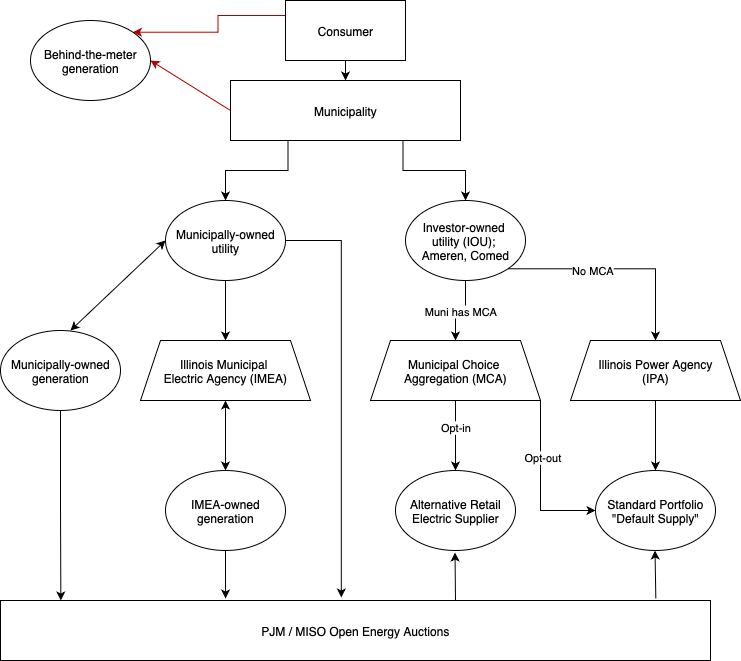
\includegraphics[width=0.75\columnwidth]{figures/07_interview_chapter/illinois-electric-choice.drawio.png}
    % \resizebox{0.75\columnwidth}{!}{\input{figures/07_interview_chapter/illinois-electric-choice.drawio.svg}}
    \caption{A flow chart describing how consumers may procure electricity in
    Illinois. \textcolor{red}{!! NOT FINAL !!}}
    \label{fig:illinois-flow-chart}
\end{figure}

Figure \ref{fig:illinois-flow-chart} shows consumers residing within
municipalities. Municipalities that own and operate a utility may obtain
electric supply by owning electric generation, participating in the energy
market, or contracting with another organization, such as the \ac{imea}, to
handle the supply procurement. In turn, \ac{imea} can procure energy by owning
generating capacity, or through the energy market. Most municipalities in
Illinois are served by one of the two major \acp{iou}, Ameren or ComEd. Due to
the Public Utilities Act of 1997, these utilities cannot profit on the supply of
electricity \cite{illinois_90th_general_assembly_electric_1997}. Rather, their
customers (consumers or municipalities) direct the utility to supply electricity
from a chosen supplier. If customers do not choose a supplier, they will receive
the default supply, procured by the \ac{ipa}. In Illinois, consumers can opt for
their municipality (where allowed) to negotiate electricity prices on their
behalf through \ac{mca}. Municipalities may either select from an \ac{ares} or
choose the default supply.\footnote{An \ac{ares} is an entity certified by the
\ac{icc} that sells electricity to customers. This electricity is generated
through privately owned resources or through purchases from the electricity
market.} Although not depicted in Figure \ref{fig:illinois-flow-chart},
consumers that reside in a municipality without \ac{mca} may still choose to
purchase electricity supply from an \ac{ares} as an individual. Of course,
consumers and municipalities may, where permitted, obtain energy by investing in
\ac{btm} resources, commonly rooftop solar panels or batteries. Municipalities
that currently outsource their electricity procurement to \ac{imea} are
contractually prohibited from building certain \ac{btm} resources.
 
% This section answers the following questions \begin{enumerate} \item Where do
% consumers get their energy from? For example, the open energy market, their
% municipality, municipal electric aggregation, or some default supply decided
% by the state of Illinois. \item How do suppliers of electricity, decide what
% types of generators in which to invest? For example, the \ac{imea} procures
% electricity on behalf of their member communities from the open market, and
% also owns part of the Prairie coal plant. \end{enumerate}

\section{Methodology}
\label{section:interview-methods}

\subsection{Thematic Analysis}
This section describes a multiple-case study using interviews with energy
planners, decision makers, and community advocates at local and state levels.
The interviewees were chosen to exemplify maximum variation cases
\cite{flyvbjerg_five_2006}. The participants and cases in this study vary in
perspective and context in order to create a holistic narrative about energy
planning within Illinois. A multiple-case study also enhances validity by
enabling replication and comparison \cite{johannsen_designing_2021,
yin_case_2018}. Further, since one purpose of this study is to evaluate the
design and applicability of the tool, \ac{osier}, a multiple-case study design
will strengthen software changes and feature additions and support \ac{osier}'s
use in other places and contexts. The raw data include interview transcriptions
and the relevant municipal climate and energy plans, if available. The
interviews were transcribed with the ``listen and revise method'' using the
Whisper transcription tool \cite{battaglia_listen_2024}. Whisper uses \ac{ai} to
automate the transcription process. Both the data and the \ac{ai} model used to
transcribe the interview audio were hosted locally (i.e., without an internet
connection), eliminating privacy concerns \cite{battaglia_listen_2024}. Figure
\ref{fig:whisper} shows a screenshot of the Whisper interface. 

\begin{figure}[htbp!]
    \centering
    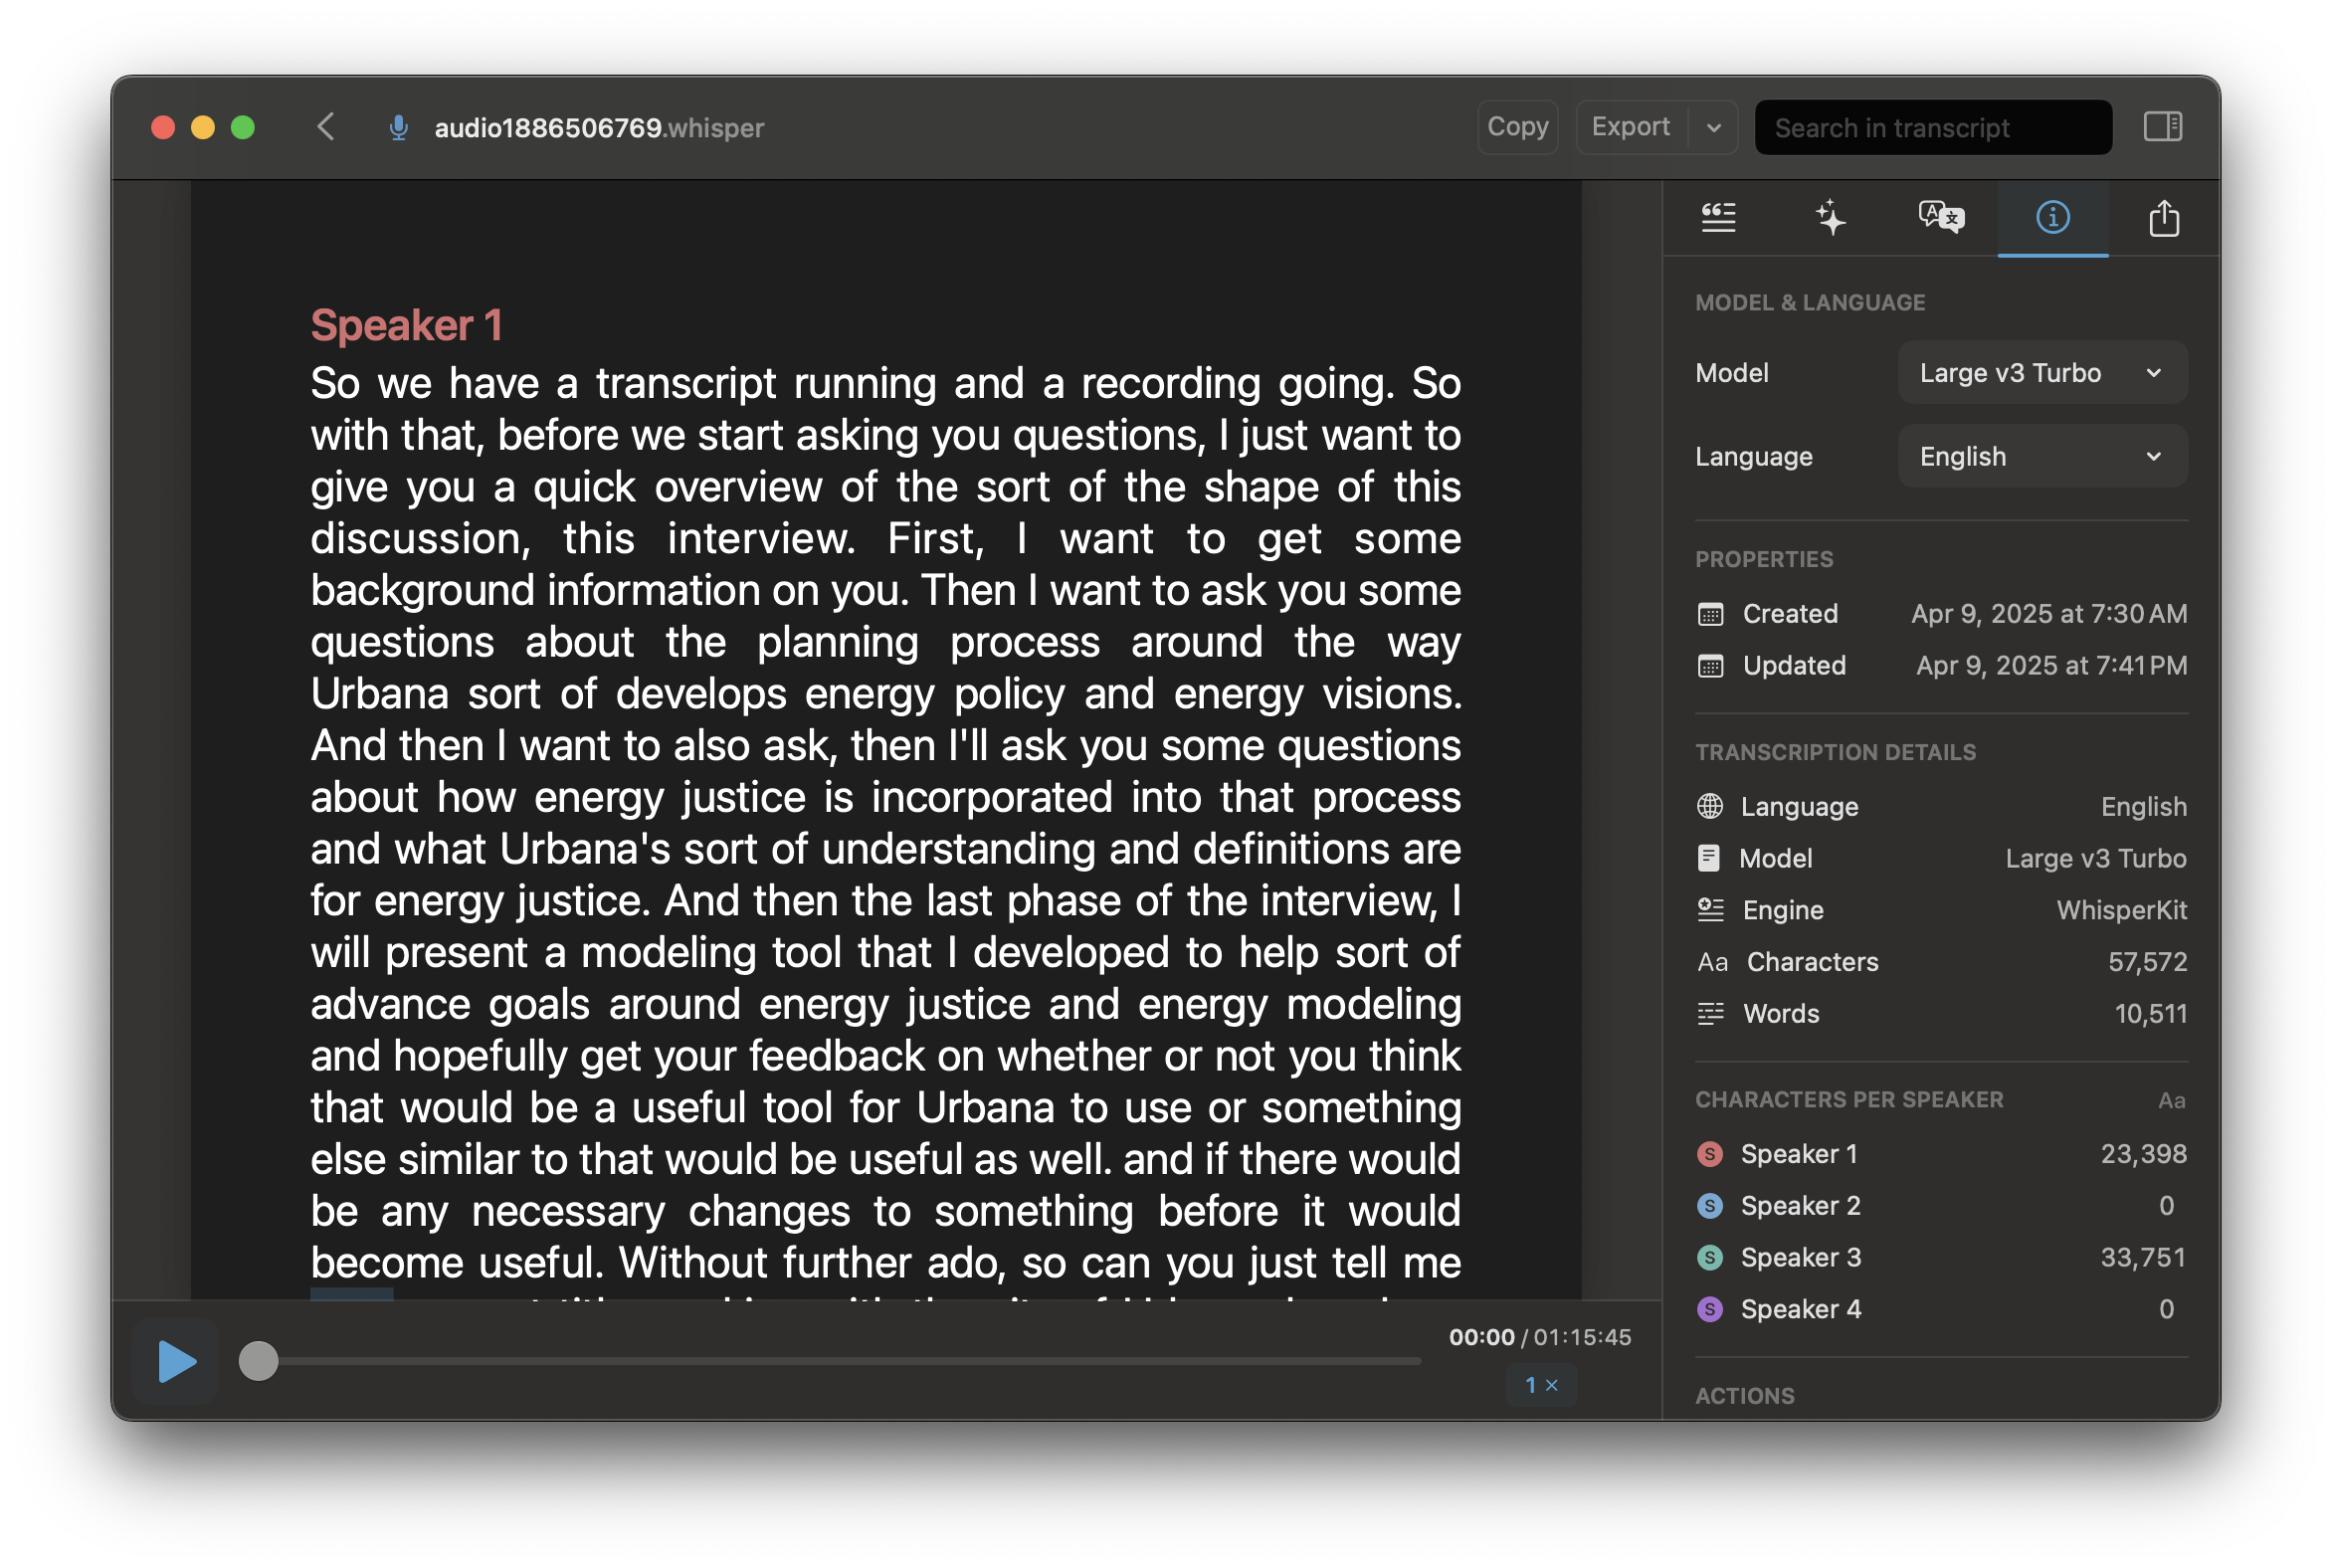
\includegraphics[width=0.75\columnwidth]{figures/07_interview_chapter/whisper-screenshot.png}
    \caption{A screenshot of an interview transcribed with Whisper. To protect
    the privacy of the interviewees, only ``Speaker 1'' is shown. ``Speaker 1''
    is the author of this thesis.}
    \label{fig:whisper}
\end{figure}

The transcribed interviews were initially coded using a deductive approach to
illuminate three aims of this study:
\begin{enumerate}
    \item identify how (if) energy models are used to support energy planning at
    local and state levels,
    \item determine the ways energy justice or equity are incorporated into
    planning decisions
    \item assess the usefulness of a new modeling tool, \ac{osier}.
\end{enumerate} 
The interview coding step was also performed locally with the \texttt{Taguette}
tool \cite{rampin_taguette_2021}. Figure \ref{fig:taguette} shows a screenshot
of the \texttt{Taguette} software.

\begin{figure}[htbp!]
    \centering
    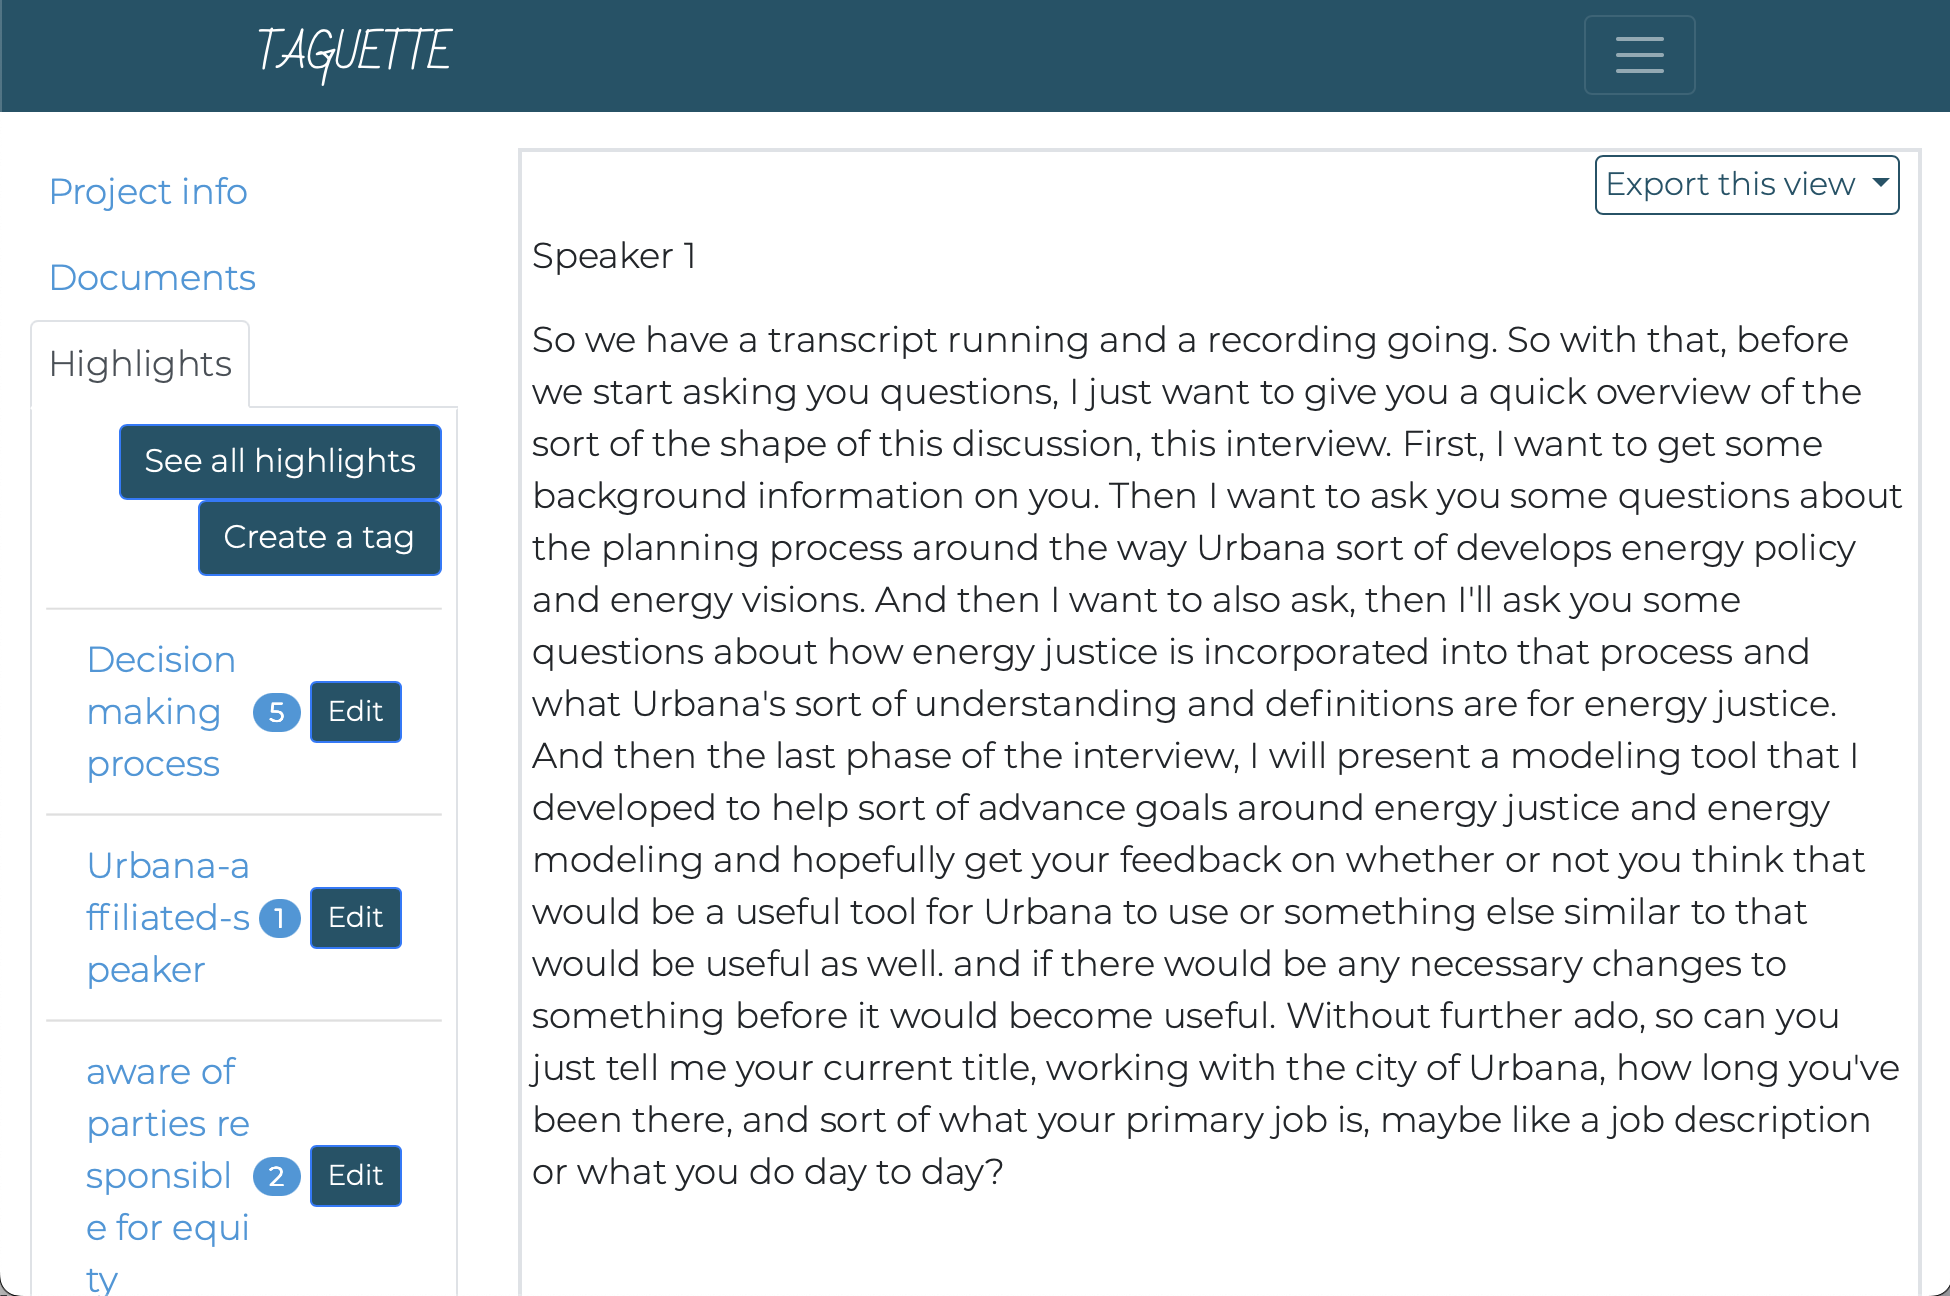
\includegraphics[width=0.75\columnwidth]{figures/07_interview_chapter/taguette-screenshot}
    \caption{A screenshot of the interview transcribed in Figure \ref{fig:whisper}
    loaded into \texttt{Taguette} for initial coding.}
    \label{fig:taguette}
\end{figure}

\subsection{Interview Data Collection}

A total of thirteen interviews were conducted virtually using the Zoom
teleconferencing software through the second half of 2024 and beginning of 2025
using a semi-structured approach based on an interview guide designed according
to five main topics (for details, see Appendix \ref{chapter:interview-guide}).
\begin{enumerate}
    \item Background --- learn about the interviewees experience and background
    with energy planning in their context.
    \item Existing planning processes --- clarify the processes used to develop
    climate action plans and energy policies.
    \item Conceptions of justice or equity --- elucidate the extent to which
    justice informs energy policies and plans.
    \item Use of models in planning processes --- identify if energy models are
    used and overall perceptions of modeling.
    \item Assessment of the \ac{osier} tool --- introduce \ac{osier} through a
    short presentation and invite reactions and feedback from the interviewee.
\end{enumerate}
The interviewees were chosen through a combination of purposive and snowball
sampling to identify staff with sufficient and relevant energy planning
experience. Each interviewee is involved in decision making, planning, or
advocacy in their respective context. 

Table \ref{tab:interviewees} summarizes the interviewees for this study. The
organization column refers to the organization that either employs, or is
represented by, the interviewee. The \textit{type} column assigns the
interviewee a broad category including
\begin{enumerate}
    \item practicioner --- someone involved in the process of energy planning
    and carries out policy directives from policy makers,
    \item advocate --- a person or organization that lobbies for policy outcomes
    on behalf of a group of stakeholders,
    \item policy maker --- someone that participates in the ultimate decision
    making related to energy policy.
\end{enumerate}
    
\begin{table}[ht!]
    \centering
    \caption{Interview participant codes and summary}
    \label{tab:interviewees}
    \begin{tabular}{llll}
        \toprule
        Number & Participant Code & Organization & Type \\
        \midrule
        1& UP1 &Urbana& Practitioner\\ % 
        2& UP2 &\ac{uiuc}/Urbana& Practitioner\\ % 
        3& UM1 &Urbana & Policy maker\\ % 
        4& UI1 & \ac{uiuc} & Practitioner\\ % 
        5& CP1 & Champaign & Practitioner\\ % 
        6& IP1 & \ac{icc} & Practitioner\\ % 
        8& IP2 & \ac{icc} & Practitioner\\ % JA
        7& IP3 & \ac{ipa} & Practitioner\\ % 
        9& IA1 &\ac{icea}& Advocate\\ % 
        10& IA2 &Illinois \ac{cub} & Advocate\\ % 
        11& NP1 & Naperville & Practitioner\\ % 
        12& NA1 &\acs{nest}&Advocate\\ % 
        13& NA2 &\acs{nest}&Advocate\\ % 
        \bottomrule
    \end{tabular}
\end{table}


\section{Case Regions}
\label{section:cases}

The case regions for this study were chosen to cover a breadth of energy
planning circumstances. Collectively, the regions cover the entire spectrum of
possibilities illustrated in Figure \ref{fig:illinois-flow-chart}. Table
\ref{tab:demographics} shows the sizes of each planning context by population.

\begin{table}[htbp!]
    \centering
    \caption{Summary demographics for the study regions from 2024.}
    \label{tab:demographics}
    \begin{tabular}{lllll}
        \toprule
        Region & Population & Operating Budget & Budget Per-Capita & Median
        Household Income \\
        & & (millions of \$) & (\$/person) &(\$/year) \\
        \midrule
        Illinois
        \cite{united_states_census_bureau_quickfacts_2024-3,sturm_illinois_2024}&
        12,710,158  & 53,419 & 4,203 & 81,702\\
        Naperville
        \cite{united_states_census_bureau_quickfacts_2024-2,munch_annual_2024} &
        150,249  & 641 & 4,266 & 150,937 \\
        Champaign
        \cite{united_states_census_bureau_quickfacts_2024,nees_adopted_2024} &
        89,189 & 210 & 2,354 & 57,544 \\
        Urbana \cite{united_states_census_bureau_quickfacts_2024-1,
        ho_city_2024}& 38,201 & 85 & 2,225 & 45,854 \\
        \ac{uiuc} \cite{data_usa_university_2022,
        university_of_illinois_system_fy_2024} & 59,916 & 3,078 & 51,371 & N/A
        \\
        \bottomrule
    \end{tabular}
\end{table}

Figure \ref{fig:illinois-plot} highlights the case study regions within a map of
Illinois. Due to their proximity, \ac{uiuc}, Champaign, and Urbana are
identified together.

\begin{figure}[ht!]
    \centering
    \resizebox{0.4\columnwidth}{!}{%% Creator: Matplotlib, PGF backend
%%
%% To include the figure in your LaTeX document, write
%%   \input{<filename>.pgf}
%%
%% Make sure the required packages are loaded in your preamble
%%   \usepackage{pgf}
%%
%% Also ensure that all the required font packages are loaded; for instance,
%% the lmodern package is sometimes necessary when using math font.
%%   \usepackage{lmodern}
%%
%% Figures using additional raster images can only be included by \input if
%% they are in the same directory as the main LaTeX file. For loading figures
%% from other directories you can use the `import` package
%%   \usepackage{import}
%%
%% and then include the figures with
%%   \import{<path to file>}{<filename>.pgf}
%%
%% Matplotlib used the following preamble
%%   \def\mathdefault#1{#1}
%%   \everymath=\expandafter{\the\everymath\displaystyle}
%%   \IfFileExists{scrextend.sty}{
%%     \usepackage[fontsize=10.000000pt]{scrextend}
%%   }{
%%     \renewcommand{\normalsize}{\fontsize{10.000000}{12.000000}\selectfont}
%%     \normalsize
%%   }
%%   
%%   \makeatletter\@ifpackageloaded{underscore}{}{\usepackage[strings]{underscore}}\makeatother
%%
\begingroup%
\makeatletter%
\begin{pgfpicture}%
\pgfpathrectangle{\pgfpointorigin}{\pgfqpoint{2.892651in}{4.700515in}}%
\pgfusepath{use as bounding box, clip}%
\begin{pgfscope}%
\pgfsetbuttcap%
\pgfsetmiterjoin%
\definecolor{currentfill}{rgb}{1.000000,1.000000,1.000000}%
\pgfsetfillcolor{currentfill}%
\pgfsetlinewidth{0.000000pt}%
\definecolor{currentstroke}{rgb}{0.000000,0.000000,0.000000}%
\pgfsetstrokecolor{currentstroke}%
\pgfsetdash{}{0pt}%
\pgfpathmoveto{\pgfqpoint{0.000000in}{0.000000in}}%
\pgfpathlineto{\pgfqpoint{2.892651in}{0.000000in}}%
\pgfpathlineto{\pgfqpoint{2.892651in}{4.700515in}}%
\pgfpathlineto{\pgfqpoint{0.000000in}{4.700515in}}%
\pgfpathlineto{\pgfqpoint{0.000000in}{0.000000in}}%
\pgfpathclose%
\pgfusepath{fill}%
\end{pgfscope}%
\begin{pgfscope}%
\pgfpathrectangle{\pgfqpoint{0.100000in}{0.100000in}}{\pgfqpoint{2.033132in}{3.747454in}}%
\pgfusepath{clip}%
\pgfsetbuttcap%
\pgfsetroundjoin%
\definecolor{currentfill}{rgb}{0.121569,0.466667,0.705882}%
\pgfsetfillcolor{currentfill}%
\pgfsetfillopacity{0.200000}%
\pgfsetlinewidth{1.003750pt}%
\definecolor{currentstroke}{rgb}{0.000000,0.000000,0.000000}%
\pgfsetstrokecolor{currentstroke}%
\pgfsetstrokeopacity{0.200000}%
\pgfsetdash{}{0pt}%
\pgfpathmoveto{\pgfqpoint{1.380005in}{2.695947in}}%
\pgfpathlineto{\pgfqpoint{1.380042in}{2.704733in}}%
\pgfpathlineto{\pgfqpoint{1.380258in}{2.731891in}}%
\pgfpathlineto{\pgfqpoint{1.380345in}{2.749927in}}%
\pgfpathlineto{\pgfqpoint{1.380373in}{2.758589in}}%
\pgfpathlineto{\pgfqpoint{1.380378in}{2.762786in}}%
\pgfpathlineto{\pgfqpoint{1.380380in}{2.767990in}}%
\pgfpathlineto{\pgfqpoint{1.380391in}{2.779925in}}%
\pgfpathlineto{\pgfqpoint{1.380364in}{2.789029in}}%
\pgfpathlineto{\pgfqpoint{1.380345in}{2.793568in}}%
\pgfpathlineto{\pgfqpoint{1.380343in}{2.795631in}}%
\pgfpathlineto{\pgfqpoint{1.380276in}{2.814327in}}%
\pgfpathlineto{\pgfqpoint{1.385644in}{2.814345in}}%
\pgfpathlineto{\pgfqpoint{1.397732in}{2.814421in}}%
\pgfpathlineto{\pgfqpoint{1.416392in}{2.814529in}}%
\pgfpathlineto{\pgfqpoint{1.417988in}{2.814524in}}%
\pgfpathlineto{\pgfqpoint{1.418169in}{2.814526in}}%
\pgfpathlineto{\pgfqpoint{1.419431in}{2.814540in}}%
\pgfpathlineto{\pgfqpoint{1.419838in}{2.814545in}}%
\pgfpathlineto{\pgfqpoint{1.420485in}{2.814552in}}%
\pgfpathlineto{\pgfqpoint{1.421633in}{2.814564in}}%
\pgfpathlineto{\pgfqpoint{1.423906in}{2.814589in}}%
\pgfpathlineto{\pgfqpoint{1.424951in}{2.814600in}}%
\pgfpathlineto{\pgfqpoint{1.425758in}{2.814609in}}%
\pgfpathlineto{\pgfqpoint{1.425843in}{2.814610in}}%
\pgfpathlineto{\pgfqpoint{1.427179in}{2.814624in}}%
\pgfpathlineto{\pgfqpoint{1.428947in}{2.814644in}}%
\pgfpathlineto{\pgfqpoint{1.429031in}{2.814645in}}%
\pgfpathlineto{\pgfqpoint{1.429329in}{2.814648in}}%
\pgfpathlineto{\pgfqpoint{1.433027in}{2.814690in}}%
\pgfpathlineto{\pgfqpoint{1.433527in}{2.814697in}}%
\pgfpathlineto{\pgfqpoint{1.434340in}{2.814703in}}%
\pgfpathlineto{\pgfqpoint{1.434867in}{2.814708in}}%
\pgfpathlineto{\pgfqpoint{1.436001in}{2.814717in}}%
\pgfpathlineto{\pgfqpoint{1.437495in}{2.814729in}}%
\pgfpathlineto{\pgfqpoint{1.460029in}{2.814854in}}%
\pgfpathlineto{\pgfqpoint{1.460036in}{2.814861in}}%
\pgfpathlineto{\pgfqpoint{1.485906in}{2.815146in}}%
\pgfpathlineto{\pgfqpoint{1.486413in}{2.815150in}}%
\pgfpathlineto{\pgfqpoint{1.487004in}{2.815144in}}%
\pgfpathlineto{\pgfqpoint{1.504178in}{2.815385in}}%
\pgfpathlineto{\pgfqpoint{1.517594in}{2.815574in}}%
\pgfpathlineto{\pgfqpoint{1.538817in}{2.815799in}}%
\pgfpathlineto{\pgfqpoint{1.539567in}{2.815809in}}%
\pgfpathlineto{\pgfqpoint{1.591834in}{2.816184in}}%
\pgfpathlineto{\pgfqpoint{1.592005in}{2.816191in}}%
\pgfpathlineto{\pgfqpoint{1.610419in}{2.816806in}}%
\pgfpathlineto{\pgfqpoint{1.613857in}{2.816907in}}%
\pgfpathlineto{\pgfqpoint{1.619380in}{2.817078in}}%
\pgfpathlineto{\pgfqpoint{1.621851in}{2.817169in}}%
\pgfpathlineto{\pgfqpoint{1.622142in}{2.817154in}}%
\pgfpathlineto{\pgfqpoint{1.623672in}{2.817224in}}%
\pgfpathlineto{\pgfqpoint{1.641448in}{2.817821in}}%
\pgfpathlineto{\pgfqpoint{1.644737in}{2.817925in}}%
\pgfpathlineto{\pgfqpoint{1.653551in}{2.818214in}}%
\pgfpathlineto{\pgfqpoint{1.657871in}{2.818366in}}%
\pgfpathlineto{\pgfqpoint{1.664199in}{2.818581in}}%
\pgfpathlineto{\pgfqpoint{1.671166in}{2.818808in}}%
\pgfpathlineto{\pgfqpoint{1.688876in}{2.819346in}}%
\pgfpathlineto{\pgfqpoint{1.692804in}{2.819444in}}%
\pgfpathlineto{\pgfqpoint{1.692964in}{2.812869in}}%
\pgfpathlineto{\pgfqpoint{1.692966in}{2.812807in}}%
\pgfpathlineto{\pgfqpoint{1.693052in}{2.809876in}}%
\pgfpathlineto{\pgfqpoint{1.693053in}{2.809793in}}%
\pgfpathlineto{\pgfqpoint{1.693066in}{2.808925in}}%
\pgfpathlineto{\pgfqpoint{1.693090in}{2.808522in}}%
\pgfpathlineto{\pgfqpoint{1.693138in}{2.806880in}}%
\pgfpathlineto{\pgfqpoint{1.693145in}{2.806618in}}%
\pgfpathlineto{\pgfqpoint{1.693817in}{2.781578in}}%
\pgfpathlineto{\pgfqpoint{1.694295in}{2.763668in}}%
\pgfpathlineto{\pgfqpoint{1.694736in}{2.745837in}}%
\pgfpathlineto{\pgfqpoint{1.695656in}{2.710195in}}%
\pgfpathlineto{\pgfqpoint{1.697026in}{2.656427in}}%
\pgfpathlineto{\pgfqpoint{1.697385in}{2.643700in}}%
\pgfpathlineto{\pgfqpoint{1.697391in}{2.643493in}}%
\pgfpathlineto{\pgfqpoint{1.697524in}{2.638617in}}%
\pgfpathlineto{\pgfqpoint{1.698260in}{2.602834in}}%
\pgfpathlineto{\pgfqpoint{1.698343in}{2.599108in}}%
\pgfpathlineto{\pgfqpoint{1.698567in}{2.589195in}}%
\pgfpathlineto{\pgfqpoint{1.698660in}{2.584964in}}%
\pgfpathlineto{\pgfqpoint{1.699070in}{2.567125in}}%
\pgfpathlineto{\pgfqpoint{1.699142in}{2.563506in}}%
\pgfpathlineto{\pgfqpoint{1.699474in}{2.549264in}}%
\pgfpathlineto{\pgfqpoint{1.699800in}{2.549269in}}%
\pgfpathlineto{\pgfqpoint{1.699840in}{2.546915in}}%
\pgfpathlineto{\pgfqpoint{1.700114in}{2.531921in}}%
\pgfpathlineto{\pgfqpoint{1.700261in}{2.523075in}}%
\pgfpathlineto{\pgfqpoint{1.700417in}{2.514326in}}%
\pgfpathlineto{\pgfqpoint{1.696880in}{2.514290in}}%
\pgfpathlineto{\pgfqpoint{1.665686in}{2.513891in}}%
\pgfpathlineto{\pgfqpoint{1.648785in}{2.513817in}}%
\pgfpathlineto{\pgfqpoint{1.648781in}{2.513607in}}%
\pgfpathlineto{\pgfqpoint{1.604858in}{2.513829in}}%
\pgfpathlineto{\pgfqpoint{1.597559in}{2.513849in}}%
\pgfpathlineto{\pgfqpoint{1.597132in}{2.513795in}}%
\pgfpathlineto{\pgfqpoint{1.548896in}{2.513320in}}%
\pgfpathlineto{\pgfqpoint{1.544217in}{2.513306in}}%
\pgfpathlineto{\pgfqpoint{1.544244in}{2.513869in}}%
\pgfpathlineto{\pgfqpoint{1.543889in}{2.546565in}}%
\pgfpathlineto{\pgfqpoint{1.543810in}{2.546639in}}%
\pgfpathlineto{\pgfqpoint{1.540609in}{2.546634in}}%
\pgfpathlineto{\pgfqpoint{1.540108in}{2.573343in}}%
\pgfpathlineto{\pgfqpoint{1.539968in}{2.582257in}}%
\pgfpathlineto{\pgfqpoint{1.539723in}{2.600077in}}%
\pgfpathlineto{\pgfqpoint{1.513443in}{2.599690in}}%
\pgfpathlineto{\pgfqpoint{1.495591in}{2.599490in}}%
\pgfpathlineto{\pgfqpoint{1.486755in}{2.599354in}}%
\pgfpathlineto{\pgfqpoint{1.482303in}{2.599284in}}%
\pgfpathlineto{\pgfqpoint{1.480266in}{2.599240in}}%
\pgfpathlineto{\pgfqpoint{1.477867in}{2.599188in}}%
\pgfpathlineto{\pgfqpoint{1.473228in}{2.599122in}}%
\pgfpathlineto{\pgfqpoint{1.460222in}{2.598872in}}%
\pgfpathlineto{\pgfqpoint{1.433819in}{2.598510in}}%
\pgfpathlineto{\pgfqpoint{1.407412in}{2.598062in}}%
\pgfpathlineto{\pgfqpoint{1.403022in}{2.597965in}}%
\pgfpathlineto{\pgfqpoint{1.380989in}{2.597450in}}%
\pgfpathlineto{\pgfqpoint{1.380552in}{2.633204in}}%
\pgfpathlineto{\pgfqpoint{1.380451in}{2.642160in}}%
\pgfpathlineto{\pgfqpoint{1.380354in}{2.651055in}}%
\pgfpathlineto{\pgfqpoint{1.380019in}{2.695744in}}%
\pgfpathlineto{\pgfqpoint{1.380005in}{2.695947in}}%
\pgfusepath{stroke,fill}%
\end{pgfscope}%
\begin{pgfscope}%
\pgfpathrectangle{\pgfqpoint{0.100000in}{0.100000in}}{\pgfqpoint{2.033132in}{3.747454in}}%
\pgfusepath{clip}%
\pgfsetbuttcap%
\pgfsetroundjoin%
\definecolor{currentfill}{rgb}{0.121569,0.466667,0.705882}%
\pgfsetfillcolor{currentfill}%
\pgfsetfillopacity{0.200000}%
\pgfsetlinewidth{1.003750pt}%
\definecolor{currentstroke}{rgb}{0.000000,0.000000,0.000000}%
\pgfsetstrokecolor{currentstroke}%
\pgfsetstrokeopacity{0.200000}%
\pgfsetdash{}{0pt}%
\pgfpathmoveto{\pgfqpoint{0.395347in}{2.954390in}}%
\pgfpathlineto{\pgfqpoint{0.395526in}{2.958117in}}%
\pgfpathlineto{\pgfqpoint{0.397841in}{2.973862in}}%
\pgfpathlineto{\pgfqpoint{0.398513in}{2.976233in}}%
\pgfpathlineto{\pgfqpoint{0.404714in}{2.986187in}}%
\pgfpathlineto{\pgfqpoint{0.404976in}{2.987586in}}%
\pgfpathlineto{\pgfqpoint{0.405289in}{2.995271in}}%
\pgfpathlineto{\pgfqpoint{0.406444in}{3.001945in}}%
\pgfpathlineto{\pgfqpoint{0.407711in}{3.004389in}}%
\pgfpathlineto{\pgfqpoint{0.408206in}{3.005019in}}%
\pgfpathlineto{\pgfqpoint{0.411360in}{3.007554in}}%
\pgfpathlineto{\pgfqpoint{0.415659in}{3.009760in}}%
\pgfpathlineto{\pgfqpoint{0.424038in}{3.010902in}}%
\pgfpathlineto{\pgfqpoint{0.425752in}{3.011317in}}%
\pgfpathlineto{\pgfqpoint{0.435389in}{3.016075in}}%
\pgfpathlineto{\pgfqpoint{0.437727in}{3.016353in}}%
\pgfpathlineto{\pgfqpoint{0.439864in}{3.016146in}}%
\pgfpathlineto{\pgfqpoint{0.443777in}{3.013726in}}%
\pgfpathlineto{\pgfqpoint{0.451538in}{3.010104in}}%
\pgfpathlineto{\pgfqpoint{0.460635in}{3.008407in}}%
\pgfpathlineto{\pgfqpoint{0.463245in}{3.009303in}}%
\pgfpathlineto{\pgfqpoint{0.465541in}{3.010981in}}%
\pgfpathlineto{\pgfqpoint{0.474633in}{3.014645in}}%
\pgfpathlineto{\pgfqpoint{0.478827in}{3.017135in}}%
\pgfpathlineto{\pgfqpoint{0.487641in}{3.023481in}}%
\pgfpathlineto{\pgfqpoint{0.489494in}{3.024900in}}%
\pgfpathlineto{\pgfqpoint{0.493969in}{3.027690in}}%
\pgfpathlineto{\pgfqpoint{0.495786in}{3.028402in}}%
\pgfpathlineto{\pgfqpoint{0.499028in}{3.029160in}}%
\pgfpathlineto{\pgfqpoint{0.503234in}{3.029457in}}%
\pgfpathlineto{\pgfqpoint{0.509066in}{3.028745in}}%
\pgfpathlineto{\pgfqpoint{0.517095in}{3.028745in}}%
\pgfpathlineto{\pgfqpoint{0.526756in}{3.027774in}}%
\pgfpathlineto{\pgfqpoint{0.530757in}{3.026773in}}%
\pgfpathlineto{\pgfqpoint{0.533477in}{3.026466in}}%
\pgfpathlineto{\pgfqpoint{0.543381in}{3.025771in}}%
\pgfpathlineto{\pgfqpoint{0.549179in}{3.026076in}}%
\pgfpathlineto{\pgfqpoint{0.555716in}{3.027395in}}%
\pgfpathlineto{\pgfqpoint{0.565914in}{3.028915in}}%
\pgfpathlineto{\pgfqpoint{0.570610in}{3.030084in}}%
\pgfpathlineto{\pgfqpoint{0.577286in}{3.032661in}}%
\pgfpathlineto{\pgfqpoint{0.581978in}{3.032538in}}%
\pgfpathlineto{\pgfqpoint{0.586762in}{3.033460in}}%
\pgfpathlineto{\pgfqpoint{0.589339in}{3.035244in}}%
\pgfpathlineto{\pgfqpoint{0.593939in}{3.040350in}}%
\pgfpathlineto{\pgfqpoint{0.598342in}{3.044190in}}%
\pgfpathlineto{\pgfqpoint{0.603922in}{3.047547in}}%
\pgfpathlineto{\pgfqpoint{0.609811in}{3.053412in}}%
\pgfpathlineto{\pgfqpoint{0.610500in}{3.054929in}}%
\pgfpathlineto{\pgfqpoint{0.611466in}{3.060465in}}%
\pgfpathlineto{\pgfqpoint{0.614967in}{3.063728in}}%
\pgfpathlineto{\pgfqpoint{0.616572in}{3.064648in}}%
\pgfpathlineto{\pgfqpoint{0.621459in}{3.066173in}}%
\pgfpathlineto{\pgfqpoint{0.625727in}{3.066801in}}%
\pgfpathlineto{\pgfqpoint{0.627957in}{3.067894in}}%
\pgfpathlineto{\pgfqpoint{0.632582in}{3.071661in}}%
\pgfpathlineto{\pgfqpoint{0.639620in}{3.072830in}}%
\pgfpathlineto{\pgfqpoint{0.643502in}{3.072002in}}%
\pgfpathlineto{\pgfqpoint{0.652409in}{3.068770in}}%
\pgfpathlineto{\pgfqpoint{0.658160in}{3.067848in}}%
\pgfpathlineto{\pgfqpoint{0.663287in}{3.067997in}}%
\pgfpathlineto{\pgfqpoint{0.670259in}{3.068893in}}%
\pgfpathlineto{\pgfqpoint{0.676193in}{3.071231in}}%
\pgfpathlineto{\pgfqpoint{0.683646in}{3.078982in}}%
\pgfpathlineto{\pgfqpoint{0.686774in}{3.083903in}}%
\pgfpathlineto{\pgfqpoint{0.689396in}{3.087225in}}%
\pgfpathlineto{\pgfqpoint{0.693166in}{3.089350in}}%
\pgfpathlineto{\pgfqpoint{0.694227in}{3.090116in}}%
\pgfpathlineto{\pgfqpoint{0.697171in}{3.095468in}}%
\pgfpathlineto{\pgfqpoint{0.698551in}{3.096944in}}%
\pgfpathlineto{\pgfqpoint{0.705405in}{3.101188in}}%
\pgfpathlineto{\pgfqpoint{0.714214in}{3.104168in}}%
\pgfpathlineto{\pgfqpoint{0.720955in}{3.105740in}}%
\pgfpathlineto{\pgfqpoint{0.730569in}{3.110785in}}%
\pgfpathlineto{\pgfqpoint{0.731561in}{3.113630in}}%
\pgfpathlineto{\pgfqpoint{0.732271in}{3.117428in}}%
\pgfpathlineto{\pgfqpoint{0.730466in}{3.147156in}}%
\pgfpathlineto{\pgfqpoint{0.733571in}{3.158073in}}%
\pgfpathlineto{\pgfqpoint{0.734878in}{3.167726in}}%
\pgfpathlineto{\pgfqpoint{0.735513in}{3.168801in}}%
\pgfpathlineto{\pgfqpoint{0.736552in}{3.169913in}}%
\pgfpathlineto{\pgfqpoint{0.742490in}{3.174659in}}%
\pgfpathlineto{\pgfqpoint{0.743698in}{3.176603in}}%
\pgfpathlineto{\pgfqpoint{0.744385in}{3.179570in}}%
\pgfpathlineto{\pgfqpoint{0.744580in}{3.181276in}}%
\pgfpathlineto{\pgfqpoint{0.744327in}{3.185624in}}%
\pgfpathlineto{\pgfqpoint{0.742441in}{3.191061in}}%
\pgfpathlineto{\pgfqpoint{0.742327in}{3.193741in}}%
\pgfpathlineto{\pgfqpoint{0.743453in}{3.200861in}}%
\pgfpathlineto{\pgfqpoint{0.745529in}{3.205751in}}%
\pgfpathlineto{\pgfqpoint{0.749175in}{3.210560in}}%
\pgfpathlineto{\pgfqpoint{0.760284in}{3.221218in}}%
\pgfpathlineto{\pgfqpoint{0.767344in}{3.224143in}}%
\pgfpathlineto{\pgfqpoint{0.769489in}{3.226101in}}%
\pgfpathlineto{\pgfqpoint{0.776961in}{3.230818in}}%
\pgfpathlineto{\pgfqpoint{0.777129in}{3.227076in}}%
\pgfpathlineto{\pgfqpoint{0.775759in}{3.223902in}}%
\pgfpathlineto{\pgfqpoint{0.775920in}{3.221243in}}%
\pgfpathlineto{\pgfqpoint{0.774721in}{3.219736in}}%
\pgfpathlineto{\pgfqpoint{0.774758in}{3.218297in}}%
\pgfpathlineto{\pgfqpoint{0.776647in}{3.218259in}}%
\pgfpathlineto{\pgfqpoint{0.777080in}{3.219653in}}%
\pgfpathlineto{\pgfqpoint{0.778000in}{3.219745in}}%
\pgfpathlineto{\pgfqpoint{0.779540in}{3.218290in}}%
\pgfpathlineto{\pgfqpoint{0.778937in}{3.217347in}}%
\pgfpathlineto{\pgfqpoint{0.776790in}{3.216667in}}%
\pgfpathlineto{\pgfqpoint{0.774967in}{3.213469in}}%
\pgfpathlineto{\pgfqpoint{0.774414in}{3.208619in}}%
\pgfpathlineto{\pgfqpoint{0.774969in}{3.207820in}}%
\pgfpathlineto{\pgfqpoint{0.776158in}{3.207826in}}%
\pgfpathlineto{\pgfqpoint{0.776598in}{3.207047in}}%
\pgfpathlineto{\pgfqpoint{0.776021in}{3.205958in}}%
\pgfpathlineto{\pgfqpoint{0.776093in}{3.204625in}}%
\pgfpathlineto{\pgfqpoint{0.777078in}{3.204697in}}%
\pgfpathlineto{\pgfqpoint{0.778319in}{3.205918in}}%
\pgfpathlineto{\pgfqpoint{0.779662in}{3.204849in}}%
\pgfpathlineto{\pgfqpoint{0.780492in}{3.201997in}}%
\pgfpathlineto{\pgfqpoint{0.779875in}{3.199372in}}%
\pgfpathlineto{\pgfqpoint{0.778664in}{3.197720in}}%
\pgfpathlineto{\pgfqpoint{0.778669in}{3.196555in}}%
\pgfpathlineto{\pgfqpoint{0.780778in}{3.195169in}}%
\pgfpathlineto{\pgfqpoint{0.780495in}{3.192372in}}%
\pgfpathlineto{\pgfqpoint{0.778355in}{3.188398in}}%
\pgfpathlineto{\pgfqpoint{0.778900in}{3.186658in}}%
\pgfpathlineto{\pgfqpoint{0.777777in}{3.185873in}}%
\pgfpathlineto{\pgfqpoint{0.778130in}{3.183897in}}%
\pgfpathlineto{\pgfqpoint{0.777059in}{3.182737in}}%
\pgfpathlineto{\pgfqpoint{0.775657in}{3.182675in}}%
\pgfpathlineto{\pgfqpoint{0.775776in}{3.181247in}}%
\pgfpathlineto{\pgfqpoint{0.777754in}{3.180044in}}%
\pgfpathlineto{\pgfqpoint{0.779365in}{3.179516in}}%
\pgfpathlineto{\pgfqpoint{0.779359in}{3.177898in}}%
\pgfpathlineto{\pgfqpoint{0.779943in}{3.177361in}}%
\pgfpathlineto{\pgfqpoint{0.780744in}{3.177818in}}%
\pgfpathlineto{\pgfqpoint{0.782123in}{3.177175in}}%
\pgfpathlineto{\pgfqpoint{0.782273in}{3.176451in}}%
\pgfpathlineto{\pgfqpoint{0.781530in}{3.175433in}}%
\pgfpathlineto{\pgfqpoint{0.781713in}{3.174777in}}%
\pgfpathlineto{\pgfqpoint{0.783546in}{3.175482in}}%
\pgfpathlineto{\pgfqpoint{0.784133in}{3.175183in}}%
\pgfpathlineto{\pgfqpoint{0.783850in}{3.172580in}}%
\pgfpathlineto{\pgfqpoint{0.784425in}{3.171752in}}%
\pgfpathlineto{\pgfqpoint{0.784101in}{3.169624in}}%
\pgfpathlineto{\pgfqpoint{0.783015in}{3.168788in}}%
\pgfpathlineto{\pgfqpoint{0.782400in}{3.169058in}}%
\pgfpathlineto{\pgfqpoint{0.781514in}{3.168387in}}%
\pgfpathlineto{\pgfqpoint{0.780389in}{3.168328in}}%
\pgfpathlineto{\pgfqpoint{0.779812in}{3.167170in}}%
\pgfpathlineto{\pgfqpoint{0.781045in}{3.165805in}}%
\pgfpathlineto{\pgfqpoint{0.782772in}{3.164635in}}%
\pgfpathlineto{\pgfqpoint{0.788934in}{3.162198in}}%
\pgfpathlineto{\pgfqpoint{0.799870in}{3.157922in}}%
\pgfpathlineto{\pgfqpoint{0.801272in}{3.157253in}}%
\pgfpathlineto{\pgfqpoint{0.804895in}{3.153875in}}%
\pgfpathlineto{\pgfqpoint{0.808555in}{3.152077in}}%
\pgfpathlineto{\pgfqpoint{0.809473in}{3.150866in}}%
\pgfpathlineto{\pgfqpoint{0.810125in}{3.148224in}}%
\pgfpathlineto{\pgfqpoint{0.812660in}{3.147605in}}%
\pgfpathlineto{\pgfqpoint{0.814006in}{3.145713in}}%
\pgfpathlineto{\pgfqpoint{0.813103in}{3.142393in}}%
\pgfpathlineto{\pgfqpoint{0.808457in}{3.142917in}}%
\pgfpathlineto{\pgfqpoint{0.808739in}{3.141414in}}%
\pgfpathlineto{\pgfqpoint{0.813723in}{3.140123in}}%
\pgfpathlineto{\pgfqpoint{0.814914in}{3.137028in}}%
\pgfpathlineto{\pgfqpoint{0.814686in}{3.134351in}}%
\pgfpathlineto{\pgfqpoint{0.813909in}{3.131533in}}%
\pgfpathlineto{\pgfqpoint{0.814541in}{3.129259in}}%
\pgfpathlineto{\pgfqpoint{0.813724in}{3.128318in}}%
\pgfpathlineto{\pgfqpoint{0.814053in}{3.127587in}}%
\pgfpathlineto{\pgfqpoint{0.812044in}{3.124299in}}%
\pgfpathlineto{\pgfqpoint{0.812531in}{3.120073in}}%
\pgfpathlineto{\pgfqpoint{0.812275in}{3.118939in}}%
\pgfpathlineto{\pgfqpoint{0.812630in}{3.116622in}}%
\pgfpathlineto{\pgfqpoint{0.812080in}{3.114677in}}%
\pgfpathlineto{\pgfqpoint{0.811294in}{3.113858in}}%
\pgfpathlineto{\pgfqpoint{0.810061in}{3.113201in}}%
\pgfpathlineto{\pgfqpoint{0.808198in}{3.112829in}}%
\pgfpathlineto{\pgfqpoint{0.805007in}{3.112728in}}%
\pgfpathlineto{\pgfqpoint{0.803966in}{3.112235in}}%
\pgfpathlineto{\pgfqpoint{0.803161in}{3.111470in}}%
\pgfpathlineto{\pgfqpoint{0.802781in}{3.109866in}}%
\pgfpathlineto{\pgfqpoint{0.803110in}{3.108780in}}%
\pgfpathlineto{\pgfqpoint{0.805633in}{3.105176in}}%
\pgfpathlineto{\pgfqpoint{0.806072in}{3.101960in}}%
\pgfpathlineto{\pgfqpoint{0.805357in}{3.097908in}}%
\pgfpathlineto{\pgfqpoint{0.803463in}{3.091184in}}%
\pgfpathlineto{\pgfqpoint{0.799908in}{3.083337in}}%
\pgfpathlineto{\pgfqpoint{0.798051in}{3.081438in}}%
\pgfpathlineto{\pgfqpoint{0.794878in}{3.080911in}}%
\pgfpathlineto{\pgfqpoint{0.791673in}{3.080719in}}%
\pgfpathlineto{\pgfqpoint{0.788757in}{3.080079in}}%
\pgfpathlineto{\pgfqpoint{0.786604in}{3.079054in}}%
\pgfpathlineto{\pgfqpoint{0.785685in}{3.077983in}}%
\pgfpathlineto{\pgfqpoint{0.785339in}{3.076081in}}%
\pgfpathlineto{\pgfqpoint{0.784569in}{3.075158in}}%
\pgfpathlineto{\pgfqpoint{0.783357in}{3.074748in}}%
\pgfpathlineto{\pgfqpoint{0.781945in}{3.074616in}}%
\pgfpathlineto{\pgfqpoint{0.777294in}{3.072026in}}%
\pgfpathlineto{\pgfqpoint{0.775457in}{3.071717in}}%
\pgfpathlineto{\pgfqpoint{0.773399in}{3.070752in}}%
\pgfpathlineto{\pgfqpoint{0.771585in}{3.070615in}}%
\pgfpathlineto{\pgfqpoint{0.768615in}{3.070001in}}%
\pgfpathlineto{\pgfqpoint{0.765026in}{3.070370in}}%
\pgfpathlineto{\pgfqpoint{0.759966in}{3.069263in}}%
\pgfpathlineto{\pgfqpoint{0.755412in}{3.069263in}}%
\pgfpathlineto{\pgfqpoint{0.751601in}{3.067914in}}%
\pgfpathlineto{\pgfqpoint{0.748285in}{3.067699in}}%
\pgfpathlineto{\pgfqpoint{0.747497in}{3.067082in}}%
\pgfpathlineto{\pgfqpoint{0.744891in}{3.063270in}}%
\pgfpathlineto{\pgfqpoint{0.743527in}{3.062417in}}%
\pgfpathlineto{\pgfqpoint{0.742228in}{3.062140in}}%
\pgfpathlineto{\pgfqpoint{0.741480in}{3.062725in}}%
\pgfpathlineto{\pgfqpoint{0.738691in}{3.063753in}}%
\pgfpathlineto{\pgfqpoint{0.735432in}{3.065367in}}%
\pgfpathlineto{\pgfqpoint{0.733577in}{3.065076in}}%
\pgfpathlineto{\pgfqpoint{0.731481in}{3.063754in}}%
\pgfpathlineto{\pgfqpoint{0.726427in}{3.062188in}}%
\pgfpathlineto{\pgfqpoint{0.723439in}{3.060528in}}%
\pgfpathlineto{\pgfqpoint{0.720909in}{3.058498in}}%
\pgfpathlineto{\pgfqpoint{0.718517in}{3.054746in}}%
\pgfpathlineto{\pgfqpoint{0.718333in}{3.052900in}}%
\pgfpathlineto{\pgfqpoint{0.717505in}{3.050563in}}%
\pgfpathlineto{\pgfqpoint{0.716170in}{3.045334in}}%
\pgfpathlineto{\pgfqpoint{0.715188in}{3.043629in}}%
\pgfpathlineto{\pgfqpoint{0.713477in}{3.042407in}}%
\pgfpathlineto{\pgfqpoint{0.710282in}{3.042258in}}%
\pgfpathlineto{\pgfqpoint{0.706024in}{3.037932in}}%
\pgfpathlineto{\pgfqpoint{0.701035in}{3.034077in}}%
\pgfpathlineto{\pgfqpoint{0.694733in}{3.030694in}}%
\pgfpathlineto{\pgfqpoint{0.689764in}{3.030201in}}%
\pgfpathlineto{\pgfqpoint{0.688933in}{2.950328in}}%
\pgfpathlineto{\pgfqpoint{0.635472in}{2.950408in}}%
\pgfpathlineto{\pgfqpoint{0.574789in}{2.951345in}}%
\pgfpathlineto{\pgfqpoint{0.532663in}{2.951749in}}%
\pgfpathlineto{\pgfqpoint{0.484062in}{2.953268in}}%
\pgfpathlineto{\pgfqpoint{0.466736in}{2.953563in}}%
\pgfpathlineto{\pgfqpoint{0.395340in}{2.954247in}}%
\pgfpathlineto{\pgfqpoint{0.395347in}{2.954390in}}%
\pgfusepath{stroke,fill}%
\end{pgfscope}%
\begin{pgfscope}%
\pgfpathrectangle{\pgfqpoint{0.100000in}{0.100000in}}{\pgfqpoint{2.033132in}{3.747454in}}%
\pgfusepath{clip}%
\pgfsetbuttcap%
\pgfsetroundjoin%
\definecolor{currentfill}{rgb}{0.121569,0.466667,0.705882}%
\pgfsetfillcolor{currentfill}%
\pgfsetfillopacity{0.200000}%
\pgfsetlinewidth{1.003750pt}%
\definecolor{currentstroke}{rgb}{0.000000,0.000000,0.000000}%
\pgfsetstrokecolor{currentstroke}%
\pgfsetstrokeopacity{0.200000}%
\pgfsetdash{}{0pt}%
\pgfpathmoveto{\pgfqpoint{0.725373in}{2.210451in}}%
\pgfpathlineto{\pgfqpoint{0.727987in}{2.211304in}}%
\pgfpathlineto{\pgfqpoint{0.728702in}{2.211867in}}%
\pgfpathlineto{\pgfqpoint{0.730352in}{2.214411in}}%
\pgfpathlineto{\pgfqpoint{0.732884in}{2.217428in}}%
\pgfpathlineto{\pgfqpoint{0.734274in}{2.218462in}}%
\pgfpathlineto{\pgfqpoint{0.736130in}{2.219181in}}%
\pgfpathlineto{\pgfqpoint{0.739888in}{2.220000in}}%
\pgfpathlineto{\pgfqpoint{0.745677in}{2.219727in}}%
\pgfpathlineto{\pgfqpoint{0.748431in}{2.220830in}}%
\pgfpathlineto{\pgfqpoint{0.753295in}{2.223939in}}%
\pgfpathlineto{\pgfqpoint{0.754939in}{2.224638in}}%
\pgfpathlineto{\pgfqpoint{0.760031in}{2.226199in}}%
\pgfpathlineto{\pgfqpoint{0.762992in}{2.228198in}}%
\pgfpathlineto{\pgfqpoint{0.765109in}{2.229118in}}%
\pgfpathlineto{\pgfqpoint{0.767273in}{2.229379in}}%
\pgfpathlineto{\pgfqpoint{0.770108in}{2.229256in}}%
\pgfpathlineto{\pgfqpoint{0.775610in}{2.228199in}}%
\pgfpathlineto{\pgfqpoint{0.777785in}{2.227251in}}%
\pgfpathlineto{\pgfqpoint{0.780298in}{2.226706in}}%
\pgfpathlineto{\pgfqpoint{0.784590in}{2.226344in}}%
\pgfpathlineto{\pgfqpoint{0.789033in}{2.226594in}}%
\pgfpathlineto{\pgfqpoint{0.790311in}{2.227105in}}%
\pgfpathlineto{\pgfqpoint{0.792052in}{2.228248in}}%
\pgfpathlineto{\pgfqpoint{0.793630in}{2.229872in}}%
\pgfpathlineto{\pgfqpoint{0.795228in}{2.232887in}}%
\pgfpathlineto{\pgfqpoint{0.795485in}{2.235579in}}%
\pgfpathlineto{\pgfqpoint{0.795222in}{2.241038in}}%
\pgfpathlineto{\pgfqpoint{0.795763in}{2.245160in}}%
\pgfpathlineto{\pgfqpoint{0.798261in}{2.250818in}}%
\pgfpathlineto{\pgfqpoint{0.799434in}{2.252193in}}%
\pgfpathlineto{\pgfqpoint{0.800250in}{2.252531in}}%
\pgfpathlineto{\pgfqpoint{0.803151in}{2.253256in}}%
\pgfpathlineto{\pgfqpoint{0.805285in}{2.254616in}}%
\pgfpathlineto{\pgfqpoint{0.806353in}{2.255773in}}%
\pgfpathlineto{\pgfqpoint{0.808029in}{2.258132in}}%
\pgfpathlineto{\pgfqpoint{0.809761in}{2.263837in}}%
\pgfpathlineto{\pgfqpoint{0.810906in}{2.265342in}}%
\pgfpathlineto{\pgfqpoint{0.815795in}{2.269159in}}%
\pgfpathlineto{\pgfqpoint{0.818307in}{2.269997in}}%
\pgfpathlineto{\pgfqpoint{0.825898in}{2.271338in}}%
\pgfpathlineto{\pgfqpoint{0.829816in}{2.273659in}}%
\pgfpathlineto{\pgfqpoint{0.833108in}{2.277687in}}%
\pgfpathlineto{\pgfqpoint{0.834344in}{2.280276in}}%
\pgfpathlineto{\pgfqpoint{0.837456in}{2.291058in}}%
\pgfpathlineto{\pgfqpoint{0.839104in}{2.294531in}}%
\pgfpathlineto{\pgfqpoint{0.840143in}{2.295870in}}%
\pgfpathlineto{\pgfqpoint{0.841237in}{2.296739in}}%
\pgfpathlineto{\pgfqpoint{0.843986in}{2.298089in}}%
\pgfpathlineto{\pgfqpoint{0.845186in}{2.299449in}}%
\pgfpathlineto{\pgfqpoint{0.846903in}{2.302038in}}%
\pgfpathlineto{\pgfqpoint{0.848938in}{2.304375in}}%
\pgfpathlineto{\pgfqpoint{0.853721in}{2.311987in}}%
\pgfpathlineto{\pgfqpoint{0.854884in}{2.313034in}}%
\pgfpathlineto{\pgfqpoint{0.856839in}{2.316184in}}%
\pgfpathlineto{\pgfqpoint{0.857019in}{2.322585in}}%
\pgfpathlineto{\pgfqpoint{0.856784in}{2.326260in}}%
\pgfpathlineto{\pgfqpoint{0.857544in}{2.328882in}}%
\pgfpathlineto{\pgfqpoint{0.858503in}{2.330390in}}%
\pgfpathlineto{\pgfqpoint{0.862902in}{2.334109in}}%
\pgfpathlineto{\pgfqpoint{0.863967in}{2.335667in}}%
\pgfpathlineto{\pgfqpoint{0.865527in}{2.341593in}}%
\pgfpathlineto{\pgfqpoint{0.865430in}{2.343264in}}%
\pgfpathlineto{\pgfqpoint{0.864173in}{2.347787in}}%
\pgfpathlineto{\pgfqpoint{0.864701in}{2.350679in}}%
\pgfpathlineto{\pgfqpoint{0.866199in}{2.354812in}}%
\pgfpathlineto{\pgfqpoint{0.868651in}{2.361659in}}%
\pgfpathlineto{\pgfqpoint{0.871003in}{2.364744in}}%
\pgfpathlineto{\pgfqpoint{0.873268in}{2.366445in}}%
\pgfpathlineto{\pgfqpoint{0.875019in}{2.367008in}}%
\pgfpathlineto{\pgfqpoint{0.878443in}{2.367791in}}%
\pgfpathlineto{\pgfqpoint{0.888408in}{2.372635in}}%
\pgfpathlineto{\pgfqpoint{0.890802in}{2.374357in}}%
\pgfpathlineto{\pgfqpoint{0.895271in}{2.375242in}}%
\pgfpathlineto{\pgfqpoint{0.895932in}{2.375567in}}%
\pgfpathlineto{\pgfqpoint{0.896957in}{2.376788in}}%
\pgfpathlineto{\pgfqpoint{0.897608in}{2.378028in}}%
\pgfpathlineto{\pgfqpoint{0.898770in}{2.381326in}}%
\pgfpathlineto{\pgfqpoint{0.899799in}{2.382849in}}%
\pgfpathlineto{\pgfqpoint{0.909080in}{2.392513in}}%
\pgfpathlineto{\pgfqpoint{0.912288in}{2.395425in}}%
\pgfpathlineto{\pgfqpoint{0.916349in}{2.398645in}}%
\pgfpathlineto{\pgfqpoint{0.918896in}{2.400168in}}%
\pgfpathlineto{\pgfqpoint{0.923109in}{2.402194in}}%
\pgfpathlineto{\pgfqpoint{0.933833in}{2.401960in}}%
\pgfpathlineto{\pgfqpoint{0.936644in}{2.402196in}}%
\pgfpathlineto{\pgfqpoint{0.952375in}{2.401833in}}%
\pgfpathlineto{\pgfqpoint{0.968096in}{2.401350in}}%
\pgfpathlineto{\pgfqpoint{0.976139in}{2.401263in}}%
\pgfpathlineto{\pgfqpoint{0.993328in}{2.401688in}}%
\pgfpathlineto{\pgfqpoint{1.003413in}{2.401650in}}%
\pgfpathlineto{\pgfqpoint{1.018598in}{2.402030in}}%
\pgfpathlineto{\pgfqpoint{1.019600in}{2.330405in}}%
\pgfpathlineto{\pgfqpoint{1.071098in}{2.330965in}}%
\pgfpathlineto{\pgfqpoint{1.072003in}{2.268395in}}%
\pgfpathlineto{\pgfqpoint{1.070813in}{2.268374in}}%
\pgfpathlineto{\pgfqpoint{1.071692in}{2.209320in}}%
\pgfpathlineto{\pgfqpoint{1.070963in}{2.208734in}}%
\pgfpathlineto{\pgfqpoint{1.069743in}{2.209549in}}%
\pgfpathlineto{\pgfqpoint{1.069523in}{2.210083in}}%
\pgfpathlineto{\pgfqpoint{1.069868in}{2.211651in}}%
\pgfpathlineto{\pgfqpoint{1.067459in}{2.212366in}}%
\pgfpathlineto{\pgfqpoint{1.067460in}{2.213120in}}%
\pgfpathlineto{\pgfqpoint{1.068263in}{2.213522in}}%
\pgfpathlineto{\pgfqpoint{1.066645in}{2.215519in}}%
\pgfpathlineto{\pgfqpoint{1.066137in}{2.216826in}}%
\pgfpathlineto{\pgfqpoint{1.064464in}{2.217571in}}%
\pgfpathlineto{\pgfqpoint{1.063134in}{2.217837in}}%
\pgfpathlineto{\pgfqpoint{1.063010in}{2.219469in}}%
\pgfpathlineto{\pgfqpoint{1.062463in}{2.220819in}}%
\pgfpathlineto{\pgfqpoint{1.061488in}{2.222107in}}%
\pgfpathlineto{\pgfqpoint{1.059828in}{2.222620in}}%
\pgfpathlineto{\pgfqpoint{1.060138in}{2.223797in}}%
\pgfpathlineto{\pgfqpoint{1.059566in}{2.224403in}}%
\pgfpathlineto{\pgfqpoint{1.059587in}{2.225584in}}%
\pgfpathlineto{\pgfqpoint{1.059031in}{2.225892in}}%
\pgfpathlineto{\pgfqpoint{1.057662in}{2.225494in}}%
\pgfpathlineto{\pgfqpoint{1.057219in}{2.227596in}}%
\pgfpathlineto{\pgfqpoint{1.056586in}{2.228510in}}%
\pgfpathlineto{\pgfqpoint{1.055628in}{2.227667in}}%
\pgfpathlineto{\pgfqpoint{1.054895in}{2.228151in}}%
\pgfpathlineto{\pgfqpoint{1.054637in}{2.229477in}}%
\pgfpathlineto{\pgfqpoint{1.053257in}{2.228892in}}%
\pgfpathlineto{\pgfqpoint{1.051127in}{2.228526in}}%
\pgfpathlineto{\pgfqpoint{1.050511in}{2.229252in}}%
\pgfpathlineto{\pgfqpoint{1.050235in}{2.230638in}}%
\pgfpathlineto{\pgfqpoint{1.049343in}{2.230732in}}%
\pgfpathlineto{\pgfqpoint{1.048872in}{2.229318in}}%
\pgfpathlineto{\pgfqpoint{1.047996in}{2.230046in}}%
\pgfpathlineto{\pgfqpoint{1.046468in}{2.230617in}}%
\pgfpathlineto{\pgfqpoint{1.045632in}{2.229950in}}%
\pgfpathlineto{\pgfqpoint{1.044552in}{2.230021in}}%
\pgfpathlineto{\pgfqpoint{1.044125in}{2.231299in}}%
\pgfpathlineto{\pgfqpoint{1.042463in}{2.232471in}}%
\pgfpathlineto{\pgfqpoint{1.040744in}{2.232871in}}%
\pgfpathlineto{\pgfqpoint{1.039868in}{2.228862in}}%
\pgfpathlineto{\pgfqpoint{1.038973in}{2.228588in}}%
\pgfpathlineto{\pgfqpoint{1.037471in}{2.228905in}}%
\pgfpathlineto{\pgfqpoint{1.035660in}{2.229677in}}%
\pgfpathlineto{\pgfqpoint{1.034858in}{2.228499in}}%
\pgfpathlineto{\pgfqpoint{1.035386in}{2.227091in}}%
\pgfpathlineto{\pgfqpoint{1.034512in}{2.227561in}}%
\pgfpathlineto{\pgfqpoint{1.033915in}{2.229391in}}%
\pgfpathlineto{\pgfqpoint{1.032936in}{2.228554in}}%
\pgfpathlineto{\pgfqpoint{1.033621in}{2.227639in}}%
\pgfpathlineto{\pgfqpoint{1.033347in}{2.226584in}}%
\pgfpathlineto{\pgfqpoint{1.032470in}{2.225895in}}%
\pgfpathlineto{\pgfqpoint{1.032593in}{2.224334in}}%
\pgfpathlineto{\pgfqpoint{1.031799in}{2.223579in}}%
\pgfpathlineto{\pgfqpoint{1.030306in}{2.223188in}}%
\pgfpathlineto{\pgfqpoint{1.030125in}{2.221732in}}%
\pgfpathlineto{\pgfqpoint{1.029563in}{2.221533in}}%
\pgfpathlineto{\pgfqpoint{1.029068in}{2.220720in}}%
\pgfpathlineto{\pgfqpoint{1.028518in}{2.220710in}}%
\pgfpathlineto{\pgfqpoint{1.027817in}{2.221505in}}%
\pgfpathlineto{\pgfqpoint{1.026142in}{2.221377in}}%
\pgfpathlineto{\pgfqpoint{1.025748in}{2.220960in}}%
\pgfpathlineto{\pgfqpoint{1.024476in}{2.220546in}}%
\pgfpathlineto{\pgfqpoint{1.024243in}{2.221990in}}%
\pgfpathlineto{\pgfqpoint{1.022989in}{2.221879in}}%
\pgfpathlineto{\pgfqpoint{1.022975in}{2.223654in}}%
\pgfpathlineto{\pgfqpoint{1.022524in}{2.224437in}}%
\pgfpathlineto{\pgfqpoint{1.021048in}{2.223796in}}%
\pgfpathlineto{\pgfqpoint{1.021038in}{2.222056in}}%
\pgfpathlineto{\pgfqpoint{1.019294in}{2.222339in}}%
\pgfpathlineto{\pgfqpoint{1.018779in}{2.221341in}}%
\pgfpathlineto{\pgfqpoint{1.017656in}{2.220361in}}%
\pgfpathlineto{\pgfqpoint{1.016230in}{2.220701in}}%
\pgfpathlineto{\pgfqpoint{1.016384in}{2.221613in}}%
\pgfpathlineto{\pgfqpoint{1.013864in}{2.221790in}}%
\pgfpathlineto{\pgfqpoint{1.013133in}{2.220840in}}%
\pgfpathlineto{\pgfqpoint{1.013622in}{2.219407in}}%
\pgfpathlineto{\pgfqpoint{1.012769in}{2.218319in}}%
\pgfpathlineto{\pgfqpoint{1.012651in}{2.217467in}}%
\pgfpathlineto{\pgfqpoint{1.012047in}{2.218543in}}%
\pgfpathlineto{\pgfqpoint{1.010795in}{2.218728in}}%
\pgfpathlineto{\pgfqpoint{1.010027in}{2.216856in}}%
\pgfpathlineto{\pgfqpoint{1.010767in}{2.216572in}}%
\pgfpathlineto{\pgfqpoint{1.010803in}{2.215698in}}%
\pgfpathlineto{\pgfqpoint{1.010049in}{2.215397in}}%
\pgfpathlineto{\pgfqpoint{1.009121in}{2.215778in}}%
\pgfpathlineto{\pgfqpoint{1.008338in}{2.214997in}}%
\pgfpathlineto{\pgfqpoint{1.006973in}{2.214905in}}%
\pgfpathlineto{\pgfqpoint{1.007384in}{2.213880in}}%
\pgfpathlineto{\pgfqpoint{1.006268in}{2.213057in}}%
\pgfpathlineto{\pgfqpoint{1.005290in}{2.213695in}}%
\pgfpathlineto{\pgfqpoint{1.003835in}{2.212072in}}%
\pgfpathlineto{\pgfqpoint{1.002991in}{2.212508in}}%
\pgfpathlineto{\pgfqpoint{1.001530in}{2.211957in}}%
\pgfpathlineto{\pgfqpoint{1.000909in}{2.212509in}}%
\pgfpathlineto{\pgfqpoint{0.999753in}{2.212466in}}%
\pgfpathlineto{\pgfqpoint{0.998308in}{2.213840in}}%
\pgfpathlineto{\pgfqpoint{0.997537in}{2.212865in}}%
\pgfpathlineto{\pgfqpoint{0.996467in}{2.213468in}}%
\pgfpathlineto{\pgfqpoint{0.995008in}{2.213538in}}%
\pgfpathlineto{\pgfqpoint{0.994262in}{2.213099in}}%
\pgfpathlineto{\pgfqpoint{0.993911in}{2.214125in}}%
\pgfpathlineto{\pgfqpoint{0.993124in}{2.214381in}}%
\pgfpathlineto{\pgfqpoint{0.992691in}{2.215378in}}%
\pgfpathlineto{\pgfqpoint{0.992143in}{2.215071in}}%
\pgfpathlineto{\pgfqpoint{0.992075in}{2.213648in}}%
\pgfpathlineto{\pgfqpoint{0.990412in}{2.213095in}}%
\pgfpathlineto{\pgfqpoint{0.989501in}{2.212206in}}%
\pgfpathlineto{\pgfqpoint{0.988678in}{2.212234in}}%
\pgfpathlineto{\pgfqpoint{0.988359in}{2.213513in}}%
\pgfpathlineto{\pgfqpoint{0.987102in}{2.213550in}}%
\pgfpathlineto{\pgfqpoint{0.985960in}{2.214043in}}%
\pgfpathlineto{\pgfqpoint{0.985287in}{2.213177in}}%
\pgfpathlineto{\pgfqpoint{0.984052in}{2.213130in}}%
\pgfpathlineto{\pgfqpoint{0.984472in}{2.211796in}}%
\pgfpathlineto{\pgfqpoint{0.983056in}{2.210198in}}%
\pgfpathlineto{\pgfqpoint{0.981724in}{2.211195in}}%
\pgfpathlineto{\pgfqpoint{0.980649in}{2.211106in}}%
\pgfpathlineto{\pgfqpoint{0.979271in}{2.210105in}}%
\pgfpathlineto{\pgfqpoint{0.978887in}{2.210794in}}%
\pgfpathlineto{\pgfqpoint{0.977706in}{2.210308in}}%
\pgfpathlineto{\pgfqpoint{0.977321in}{2.210863in}}%
\pgfpathlineto{\pgfqpoint{0.976066in}{2.210681in}}%
\pgfpathlineto{\pgfqpoint{0.975540in}{2.210194in}}%
\pgfpathlineto{\pgfqpoint{0.976447in}{2.208841in}}%
\pgfpathlineto{\pgfqpoint{0.975829in}{2.208604in}}%
\pgfpathlineto{\pgfqpoint{0.974374in}{2.209170in}}%
\pgfpathlineto{\pgfqpoint{0.973703in}{2.210563in}}%
\pgfpathlineto{\pgfqpoint{0.971751in}{2.211150in}}%
\pgfpathlineto{\pgfqpoint{0.971206in}{2.209589in}}%
\pgfpathlineto{\pgfqpoint{0.970256in}{2.210000in}}%
\pgfpathlineto{\pgfqpoint{0.969452in}{2.209661in}}%
\pgfpathlineto{\pgfqpoint{0.969482in}{2.208756in}}%
\pgfpathlineto{\pgfqpoint{0.967836in}{2.211357in}}%
\pgfpathlineto{\pgfqpoint{0.967137in}{2.211350in}}%
\pgfpathlineto{\pgfqpoint{0.966319in}{2.210960in}}%
\pgfpathlineto{\pgfqpoint{0.965995in}{2.210070in}}%
\pgfpathlineto{\pgfqpoint{0.964833in}{2.210572in}}%
\pgfpathlineto{\pgfqpoint{0.964254in}{2.212146in}}%
\pgfpathlineto{\pgfqpoint{0.963348in}{2.212576in}}%
\pgfpathlineto{\pgfqpoint{0.963393in}{2.213602in}}%
\pgfpathlineto{\pgfqpoint{0.962931in}{2.214217in}}%
\pgfpathlineto{\pgfqpoint{0.961723in}{2.214393in}}%
\pgfpathlineto{\pgfqpoint{0.961371in}{2.213885in}}%
\pgfpathlineto{\pgfqpoint{0.961109in}{2.212197in}}%
\pgfpathlineto{\pgfqpoint{0.960565in}{2.211774in}}%
\pgfpathlineto{\pgfqpoint{0.958683in}{2.212536in}}%
\pgfpathlineto{\pgfqpoint{0.956492in}{2.214004in}}%
\pgfpathlineto{\pgfqpoint{0.955273in}{2.214106in}}%
\pgfpathlineto{\pgfqpoint{0.953740in}{2.213431in}}%
\pgfpathlineto{\pgfqpoint{0.952676in}{2.213977in}}%
\pgfpathlineto{\pgfqpoint{0.950852in}{2.212704in}}%
\pgfpathlineto{\pgfqpoint{0.949492in}{2.213244in}}%
\pgfpathlineto{\pgfqpoint{0.949068in}{2.213836in}}%
\pgfpathlineto{\pgfqpoint{0.949401in}{2.215690in}}%
\pgfpathlineto{\pgfqpoint{0.948006in}{2.218120in}}%
\pgfpathlineto{\pgfqpoint{0.947088in}{2.218570in}}%
\pgfpathlineto{\pgfqpoint{0.945912in}{2.218025in}}%
\pgfpathlineto{\pgfqpoint{0.944827in}{2.216399in}}%
\pgfpathlineto{\pgfqpoint{0.944170in}{2.216213in}}%
\pgfpathlineto{\pgfqpoint{0.943095in}{2.216478in}}%
\pgfpathlineto{\pgfqpoint{0.943307in}{2.217438in}}%
\pgfpathlineto{\pgfqpoint{0.942768in}{2.217915in}}%
\pgfpathlineto{\pgfqpoint{0.940974in}{2.216798in}}%
\pgfpathlineto{\pgfqpoint{0.941774in}{2.215029in}}%
\pgfpathlineto{\pgfqpoint{0.941783in}{2.213511in}}%
\pgfpathlineto{\pgfqpoint{0.941380in}{2.212909in}}%
\pgfpathlineto{\pgfqpoint{0.940329in}{2.213079in}}%
\pgfpathlineto{\pgfqpoint{0.939160in}{2.214149in}}%
\pgfpathlineto{\pgfqpoint{0.938248in}{2.214342in}}%
\pgfpathlineto{\pgfqpoint{0.936169in}{2.213442in}}%
\pgfpathlineto{\pgfqpoint{0.935328in}{2.212652in}}%
\pgfpathlineto{\pgfqpoint{0.934478in}{2.213321in}}%
\pgfpathlineto{\pgfqpoint{0.933610in}{2.215376in}}%
\pgfpathlineto{\pgfqpoint{0.932753in}{2.216492in}}%
\pgfpathlineto{\pgfqpoint{0.931784in}{2.217173in}}%
\pgfpathlineto{\pgfqpoint{0.931399in}{2.218046in}}%
\pgfpathlineto{\pgfqpoint{0.930598in}{2.218798in}}%
\pgfpathlineto{\pgfqpoint{0.930273in}{2.217269in}}%
\pgfpathlineto{\pgfqpoint{0.931542in}{2.216080in}}%
\pgfpathlineto{\pgfqpoint{0.930991in}{2.214999in}}%
\pgfpathlineto{\pgfqpoint{0.930034in}{2.215094in}}%
\pgfpathlineto{\pgfqpoint{0.926975in}{2.216179in}}%
\pgfpathlineto{\pgfqpoint{0.926324in}{2.217470in}}%
\pgfpathlineto{\pgfqpoint{0.925308in}{2.217857in}}%
\pgfpathlineto{\pgfqpoint{0.924902in}{2.219226in}}%
\pgfpathlineto{\pgfqpoint{0.923908in}{2.219013in}}%
\pgfpathlineto{\pgfqpoint{0.923586in}{2.217648in}}%
\pgfpathlineto{\pgfqpoint{0.922958in}{2.217932in}}%
\pgfpathlineto{\pgfqpoint{0.923032in}{2.219062in}}%
\pgfpathlineto{\pgfqpoint{0.922475in}{2.220129in}}%
\pgfpathlineto{\pgfqpoint{0.921300in}{2.220062in}}%
\pgfpathlineto{\pgfqpoint{0.920188in}{2.218669in}}%
\pgfpathlineto{\pgfqpoint{0.919637in}{2.218472in}}%
\pgfpathlineto{\pgfqpoint{0.918514in}{2.218791in}}%
\pgfpathlineto{\pgfqpoint{0.915336in}{2.218158in}}%
\pgfpathlineto{\pgfqpoint{0.915989in}{2.217061in}}%
\pgfpathlineto{\pgfqpoint{0.917608in}{2.216280in}}%
\pgfpathlineto{\pgfqpoint{0.917362in}{2.215246in}}%
\pgfpathlineto{\pgfqpoint{0.915125in}{2.214961in}}%
\pgfpathlineto{\pgfqpoint{0.914888in}{2.216328in}}%
\pgfpathlineto{\pgfqpoint{0.913806in}{2.216283in}}%
\pgfpathlineto{\pgfqpoint{0.913828in}{2.214747in}}%
\pgfpathlineto{\pgfqpoint{0.913542in}{2.214302in}}%
\pgfpathlineto{\pgfqpoint{0.912299in}{2.214676in}}%
\pgfpathlineto{\pgfqpoint{0.912066in}{2.215423in}}%
\pgfpathlineto{\pgfqpoint{0.911994in}{2.217293in}}%
\pgfpathlineto{\pgfqpoint{0.911176in}{2.217366in}}%
\pgfpathlineto{\pgfqpoint{0.910778in}{2.215270in}}%
\pgfpathlineto{\pgfqpoint{0.910258in}{2.215687in}}%
\pgfpathlineto{\pgfqpoint{0.910201in}{2.216631in}}%
\pgfpathlineto{\pgfqpoint{0.909551in}{2.218081in}}%
\pgfpathlineto{\pgfqpoint{0.908286in}{2.218246in}}%
\pgfpathlineto{\pgfqpoint{0.907742in}{2.216802in}}%
\pgfpathlineto{\pgfqpoint{0.907380in}{2.216691in}}%
\pgfpathlineto{\pgfqpoint{0.906752in}{2.219422in}}%
\pgfpathlineto{\pgfqpoint{0.905929in}{2.219434in}}%
\pgfpathlineto{\pgfqpoint{0.905466in}{2.220307in}}%
\pgfpathlineto{\pgfqpoint{0.905444in}{2.222034in}}%
\pgfpathlineto{\pgfqpoint{0.904013in}{2.222049in}}%
\pgfpathlineto{\pgfqpoint{0.903476in}{2.221751in}}%
\pgfpathlineto{\pgfqpoint{0.902036in}{2.221441in}}%
\pgfpathlineto{\pgfqpoint{0.901745in}{2.220694in}}%
\pgfpathlineto{\pgfqpoint{0.902393in}{2.219037in}}%
\pgfpathlineto{\pgfqpoint{0.901975in}{2.218648in}}%
\pgfpathlineto{\pgfqpoint{0.901079in}{2.218692in}}%
\pgfpathlineto{\pgfqpoint{0.900143in}{2.217518in}}%
\pgfpathlineto{\pgfqpoint{0.900427in}{2.216833in}}%
\pgfpathlineto{\pgfqpoint{0.901391in}{2.216674in}}%
\pgfpathlineto{\pgfqpoint{0.901549in}{2.215821in}}%
\pgfpathlineto{\pgfqpoint{0.900985in}{2.215305in}}%
\pgfpathlineto{\pgfqpoint{0.899850in}{2.214923in}}%
\pgfpathlineto{\pgfqpoint{0.899186in}{2.214238in}}%
\pgfpathlineto{\pgfqpoint{0.899585in}{2.213423in}}%
\pgfpathlineto{\pgfqpoint{0.900660in}{2.213031in}}%
\pgfpathlineto{\pgfqpoint{0.900445in}{2.212244in}}%
\pgfpathlineto{\pgfqpoint{0.899484in}{2.212013in}}%
\pgfpathlineto{\pgfqpoint{0.898265in}{2.210960in}}%
\pgfpathlineto{\pgfqpoint{0.896866in}{2.212937in}}%
\pgfpathlineto{\pgfqpoint{0.895394in}{2.213597in}}%
\pgfpathlineto{\pgfqpoint{0.894602in}{2.213397in}}%
\pgfpathlineto{\pgfqpoint{0.894598in}{2.212504in}}%
\pgfpathlineto{\pgfqpoint{0.895587in}{2.210512in}}%
\pgfpathlineto{\pgfqpoint{0.895450in}{2.209823in}}%
\pgfpathlineto{\pgfqpoint{0.894677in}{2.209571in}}%
\pgfpathlineto{\pgfqpoint{0.894118in}{2.210284in}}%
\pgfpathlineto{\pgfqpoint{0.893645in}{2.209723in}}%
\pgfpathlineto{\pgfqpoint{0.894005in}{2.208847in}}%
\pgfpathlineto{\pgfqpoint{0.894004in}{2.207643in}}%
\pgfpathlineto{\pgfqpoint{0.893660in}{2.206862in}}%
\pgfpathlineto{\pgfqpoint{0.894171in}{2.205723in}}%
\pgfpathlineto{\pgfqpoint{0.896046in}{2.205486in}}%
\pgfpathlineto{\pgfqpoint{0.896437in}{2.205007in}}%
\pgfpathlineto{\pgfqpoint{0.896203in}{2.203793in}}%
\pgfpathlineto{\pgfqpoint{0.894982in}{2.202907in}}%
\pgfpathlineto{\pgfqpoint{0.892054in}{2.202888in}}%
\pgfpathlineto{\pgfqpoint{0.891489in}{2.202218in}}%
\pgfpathlineto{\pgfqpoint{0.891871in}{2.201173in}}%
\pgfpathlineto{\pgfqpoint{0.891252in}{2.200479in}}%
\pgfpathlineto{\pgfqpoint{0.890719in}{2.201034in}}%
\pgfpathlineto{\pgfqpoint{0.890724in}{2.202226in}}%
\pgfpathlineto{\pgfqpoint{0.889779in}{2.203435in}}%
\pgfpathlineto{\pgfqpoint{0.889427in}{2.202145in}}%
\pgfpathlineto{\pgfqpoint{0.888574in}{2.200531in}}%
\pgfpathlineto{\pgfqpoint{0.888545in}{2.197601in}}%
\pgfpathlineto{\pgfqpoint{0.887544in}{2.197782in}}%
\pgfpathlineto{\pgfqpoint{0.887069in}{2.199481in}}%
\pgfpathlineto{\pgfqpoint{0.886938in}{2.201248in}}%
\pgfpathlineto{\pgfqpoint{0.886198in}{2.201086in}}%
\pgfpathlineto{\pgfqpoint{0.885669in}{2.200228in}}%
\pgfpathlineto{\pgfqpoint{0.885762in}{2.198323in}}%
\pgfpathlineto{\pgfqpoint{0.884771in}{2.197607in}}%
\pgfpathlineto{\pgfqpoint{0.883606in}{2.197945in}}%
\pgfpathlineto{\pgfqpoint{0.883199in}{2.197342in}}%
\pgfpathlineto{\pgfqpoint{0.883068in}{2.196175in}}%
\pgfpathlineto{\pgfqpoint{0.882543in}{2.196068in}}%
\pgfpathlineto{\pgfqpoint{0.882138in}{2.197206in}}%
\pgfpathlineto{\pgfqpoint{0.881462in}{2.197410in}}%
\pgfpathlineto{\pgfqpoint{0.881065in}{2.196872in}}%
\pgfpathlineto{\pgfqpoint{0.880320in}{2.196850in}}%
\pgfpathlineto{\pgfqpoint{0.879901in}{2.197545in}}%
\pgfpathlineto{\pgfqpoint{0.878900in}{2.197762in}}%
\pgfpathlineto{\pgfqpoint{0.879323in}{2.198397in}}%
\pgfpathlineto{\pgfqpoint{0.879170in}{2.199029in}}%
\pgfpathlineto{\pgfqpoint{0.877619in}{2.198458in}}%
\pgfpathlineto{\pgfqpoint{0.876292in}{2.198890in}}%
\pgfpathlineto{\pgfqpoint{0.873799in}{2.198930in}}%
\pgfpathlineto{\pgfqpoint{0.873601in}{2.199302in}}%
\pgfpathlineto{\pgfqpoint{0.874222in}{2.200915in}}%
\pgfpathlineto{\pgfqpoint{0.874200in}{2.202040in}}%
\pgfpathlineto{\pgfqpoint{0.873780in}{2.202148in}}%
\pgfpathlineto{\pgfqpoint{0.872346in}{2.200607in}}%
\pgfpathlineto{\pgfqpoint{0.871258in}{2.197654in}}%
\pgfpathlineto{\pgfqpoint{0.870422in}{2.197134in}}%
\pgfpathlineto{\pgfqpoint{0.870375in}{2.200048in}}%
\pgfpathlineto{\pgfqpoint{0.869596in}{2.201114in}}%
\pgfpathlineto{\pgfqpoint{0.868478in}{2.200971in}}%
\pgfpathlineto{\pgfqpoint{0.865970in}{2.198753in}}%
\pgfpathlineto{\pgfqpoint{0.864896in}{2.196991in}}%
\pgfpathlineto{\pgfqpoint{0.864942in}{2.195334in}}%
\pgfpathlineto{\pgfqpoint{0.864083in}{2.195019in}}%
\pgfpathlineto{\pgfqpoint{0.862618in}{2.195764in}}%
\pgfpathlineto{\pgfqpoint{0.861109in}{2.195710in}}%
\pgfpathlineto{\pgfqpoint{0.859534in}{2.196072in}}%
\pgfpathlineto{\pgfqpoint{0.858715in}{2.195643in}}%
\pgfpathlineto{\pgfqpoint{0.858184in}{2.193667in}}%
\pgfpathlineto{\pgfqpoint{0.858479in}{2.192381in}}%
\pgfpathlineto{\pgfqpoint{0.858222in}{2.191468in}}%
\pgfpathlineto{\pgfqpoint{0.857576in}{2.191427in}}%
\pgfpathlineto{\pgfqpoint{0.856310in}{2.191927in}}%
\pgfpathlineto{\pgfqpoint{0.855435in}{2.191817in}}%
\pgfpathlineto{\pgfqpoint{0.855542in}{2.191056in}}%
\pgfpathlineto{\pgfqpoint{0.856239in}{2.190069in}}%
\pgfpathlineto{\pgfqpoint{0.856159in}{2.189396in}}%
\pgfpathlineto{\pgfqpoint{0.854322in}{2.189537in}}%
\pgfpathlineto{\pgfqpoint{0.851956in}{2.187713in}}%
\pgfpathlineto{\pgfqpoint{0.852696in}{2.186937in}}%
\pgfpathlineto{\pgfqpoint{0.852521in}{2.186523in}}%
\pgfpathlineto{\pgfqpoint{0.851565in}{2.186800in}}%
\pgfpathlineto{\pgfqpoint{0.851134in}{2.186275in}}%
\pgfpathlineto{\pgfqpoint{0.851631in}{2.185182in}}%
\pgfpathlineto{\pgfqpoint{0.851633in}{2.183825in}}%
\pgfpathlineto{\pgfqpoint{0.851104in}{2.183302in}}%
\pgfpathlineto{\pgfqpoint{0.847982in}{2.185711in}}%
\pgfpathlineto{\pgfqpoint{0.847739in}{2.185047in}}%
\pgfpathlineto{\pgfqpoint{0.848196in}{2.184065in}}%
\pgfpathlineto{\pgfqpoint{0.848155in}{2.183138in}}%
\pgfpathlineto{\pgfqpoint{0.847334in}{2.183679in}}%
\pgfpathlineto{\pgfqpoint{0.846499in}{2.183596in}}%
\pgfpathlineto{\pgfqpoint{0.845744in}{2.182089in}}%
\pgfpathlineto{\pgfqpoint{0.845030in}{2.181467in}}%
\pgfpathlineto{\pgfqpoint{0.844182in}{2.181897in}}%
\pgfpathlineto{\pgfqpoint{0.845382in}{2.183556in}}%
\pgfpathlineto{\pgfqpoint{0.844560in}{2.183902in}}%
\pgfpathlineto{\pgfqpoint{0.842849in}{2.181926in}}%
\pgfpathlineto{\pgfqpoint{0.841762in}{2.181991in}}%
\pgfpathlineto{\pgfqpoint{0.841274in}{2.183391in}}%
\pgfpathlineto{\pgfqpoint{0.840467in}{2.183462in}}%
\pgfpathlineto{\pgfqpoint{0.840183in}{2.182272in}}%
\pgfpathlineto{\pgfqpoint{0.839443in}{2.182065in}}%
\pgfpathlineto{\pgfqpoint{0.838489in}{2.182950in}}%
\pgfpathlineto{\pgfqpoint{0.837854in}{2.182163in}}%
\pgfpathlineto{\pgfqpoint{0.836508in}{2.183865in}}%
\pgfpathlineto{\pgfqpoint{0.835916in}{2.183229in}}%
\pgfpathlineto{\pgfqpoint{0.835014in}{2.183714in}}%
\pgfpathlineto{\pgfqpoint{0.835094in}{2.182428in}}%
\pgfpathlineto{\pgfqpoint{0.833734in}{2.181916in}}%
\pgfpathlineto{\pgfqpoint{0.832522in}{2.181115in}}%
\pgfpathlineto{\pgfqpoint{0.832037in}{2.181710in}}%
\pgfpathlineto{\pgfqpoint{0.830947in}{2.181655in}}%
\pgfpathlineto{\pgfqpoint{0.830152in}{2.181171in}}%
\pgfpathlineto{\pgfqpoint{0.829976in}{2.180273in}}%
\pgfpathlineto{\pgfqpoint{0.829222in}{2.179498in}}%
\pgfpathlineto{\pgfqpoint{0.829182in}{2.178738in}}%
\pgfpathlineto{\pgfqpoint{0.828494in}{2.177618in}}%
\pgfpathlineto{\pgfqpoint{0.828621in}{2.176386in}}%
\pgfpathlineto{\pgfqpoint{0.827282in}{2.176194in}}%
\pgfpathlineto{\pgfqpoint{0.827699in}{2.174934in}}%
\pgfpathlineto{\pgfqpoint{0.826891in}{2.173995in}}%
\pgfpathlineto{\pgfqpoint{0.826433in}{2.172335in}}%
\pgfpathlineto{\pgfqpoint{0.824441in}{2.172999in}}%
\pgfpathlineto{\pgfqpoint{0.824925in}{2.173829in}}%
\pgfpathlineto{\pgfqpoint{0.824859in}{2.174631in}}%
\pgfpathlineto{\pgfqpoint{0.824145in}{2.174576in}}%
\pgfpathlineto{\pgfqpoint{0.823559in}{2.173639in}}%
\pgfpathlineto{\pgfqpoint{0.822664in}{2.173692in}}%
\pgfpathlineto{\pgfqpoint{0.821816in}{2.175047in}}%
\pgfpathlineto{\pgfqpoint{0.819339in}{2.175615in}}%
\pgfpathlineto{\pgfqpoint{0.819595in}{2.174135in}}%
\pgfpathlineto{\pgfqpoint{0.818587in}{2.174763in}}%
\pgfpathlineto{\pgfqpoint{0.817576in}{2.174786in}}%
\pgfpathlineto{\pgfqpoint{0.816536in}{2.171696in}}%
\pgfpathlineto{\pgfqpoint{0.815732in}{2.172628in}}%
\pgfpathlineto{\pgfqpoint{0.814868in}{2.172804in}}%
\pgfpathlineto{\pgfqpoint{0.814594in}{2.171459in}}%
\pgfpathlineto{\pgfqpoint{0.811334in}{2.171447in}}%
\pgfpathlineto{\pgfqpoint{0.810531in}{2.170751in}}%
\pgfpathlineto{\pgfqpoint{0.810133in}{2.171952in}}%
\pgfpathlineto{\pgfqpoint{0.809158in}{2.171985in}}%
\pgfpathlineto{\pgfqpoint{0.808709in}{2.171223in}}%
\pgfpathlineto{\pgfqpoint{0.807280in}{2.171031in}}%
\pgfpathlineto{\pgfqpoint{0.806881in}{2.171565in}}%
\pgfpathlineto{\pgfqpoint{0.806617in}{2.172914in}}%
\pgfpathlineto{\pgfqpoint{0.805809in}{2.173323in}}%
\pgfpathlineto{\pgfqpoint{0.804326in}{2.172536in}}%
\pgfpathlineto{\pgfqpoint{0.804205in}{2.172947in}}%
\pgfpathlineto{\pgfqpoint{0.804887in}{2.174722in}}%
\pgfpathlineto{\pgfqpoint{0.804432in}{2.175246in}}%
\pgfpathlineto{\pgfqpoint{0.803727in}{2.175027in}}%
\pgfpathlineto{\pgfqpoint{0.803513in}{2.173779in}}%
\pgfpathlineto{\pgfqpoint{0.802873in}{2.173664in}}%
\pgfpathlineto{\pgfqpoint{0.802047in}{2.174490in}}%
\pgfpathlineto{\pgfqpoint{0.801298in}{2.174300in}}%
\pgfpathlineto{\pgfqpoint{0.801369in}{2.173875in}}%
\pgfpathlineto{\pgfqpoint{0.802668in}{2.172805in}}%
\pgfpathlineto{\pgfqpoint{0.802761in}{2.171961in}}%
\pgfpathlineto{\pgfqpoint{0.801612in}{2.171683in}}%
\pgfpathlineto{\pgfqpoint{0.801249in}{2.170986in}}%
\pgfpathlineto{\pgfqpoint{0.800079in}{2.170942in}}%
\pgfpathlineto{\pgfqpoint{0.799944in}{2.169300in}}%
\pgfpathlineto{\pgfqpoint{0.798788in}{2.168626in}}%
\pgfpathlineto{\pgfqpoint{0.798910in}{2.167116in}}%
\pgfpathlineto{\pgfqpoint{0.797441in}{2.166896in}}%
\pgfpathlineto{\pgfqpoint{0.795729in}{2.167276in}}%
\pgfpathlineto{\pgfqpoint{0.794780in}{2.166586in}}%
\pgfpathlineto{\pgfqpoint{0.794203in}{2.167473in}}%
\pgfpathlineto{\pgfqpoint{0.793311in}{2.168103in}}%
\pgfpathlineto{\pgfqpoint{0.793303in}{2.168968in}}%
\pgfpathlineto{\pgfqpoint{0.793709in}{2.170661in}}%
\pgfpathlineto{\pgfqpoint{0.793345in}{2.171094in}}%
\pgfpathlineto{\pgfqpoint{0.792503in}{2.170734in}}%
\pgfpathlineto{\pgfqpoint{0.791977in}{2.168799in}}%
\pgfpathlineto{\pgfqpoint{0.791171in}{2.168066in}}%
\pgfpathlineto{\pgfqpoint{0.790885in}{2.168535in}}%
\pgfpathlineto{\pgfqpoint{0.791063in}{2.170227in}}%
\pgfpathlineto{\pgfqpoint{0.790328in}{2.170469in}}%
\pgfpathlineto{\pgfqpoint{0.789060in}{2.168694in}}%
\pgfpathlineto{\pgfqpoint{0.789716in}{2.168196in}}%
\pgfpathlineto{\pgfqpoint{0.789110in}{2.167360in}}%
\pgfpathlineto{\pgfqpoint{0.788940in}{2.165711in}}%
\pgfpathlineto{\pgfqpoint{0.788127in}{2.165571in}}%
\pgfpathlineto{\pgfqpoint{0.787513in}{2.167257in}}%
\pgfpathlineto{\pgfqpoint{0.786007in}{2.167916in}}%
\pgfpathlineto{\pgfqpoint{0.784758in}{2.167857in}}%
\pgfpathlineto{\pgfqpoint{0.784124in}{2.167306in}}%
\pgfpathlineto{\pgfqpoint{0.784168in}{2.166097in}}%
\pgfpathlineto{\pgfqpoint{0.783619in}{2.165752in}}%
\pgfpathlineto{\pgfqpoint{0.782983in}{2.167342in}}%
\pgfpathlineto{\pgfqpoint{0.783089in}{2.168419in}}%
\pgfpathlineto{\pgfqpoint{0.782689in}{2.169086in}}%
\pgfpathlineto{\pgfqpoint{0.781762in}{2.169078in}}%
\pgfpathlineto{\pgfqpoint{0.779999in}{2.169898in}}%
\pgfpathlineto{\pgfqpoint{0.780769in}{2.171503in}}%
\pgfpathlineto{\pgfqpoint{0.779998in}{2.171532in}}%
\pgfpathlineto{\pgfqpoint{0.778430in}{2.169780in}}%
\pgfpathlineto{\pgfqpoint{0.776419in}{2.169653in}}%
\pgfpathlineto{\pgfqpoint{0.776026in}{2.170510in}}%
\pgfpathlineto{\pgfqpoint{0.776489in}{2.171522in}}%
\pgfpathlineto{\pgfqpoint{0.775798in}{2.171566in}}%
\pgfpathlineto{\pgfqpoint{0.774749in}{2.170120in}}%
\pgfpathlineto{\pgfqpoint{0.774694in}{2.168845in}}%
\pgfpathlineto{\pgfqpoint{0.773915in}{2.169687in}}%
\pgfpathlineto{\pgfqpoint{0.773203in}{2.169855in}}%
\pgfpathlineto{\pgfqpoint{0.772382in}{2.169202in}}%
\pgfpathlineto{\pgfqpoint{0.771622in}{2.169161in}}%
\pgfpathlineto{\pgfqpoint{0.770384in}{2.170285in}}%
\pgfpathlineto{\pgfqpoint{0.768679in}{2.170488in}}%
\pgfpathlineto{\pgfqpoint{0.768306in}{2.171888in}}%
\pgfpathlineto{\pgfqpoint{0.766702in}{2.171637in}}%
\pgfpathlineto{\pgfqpoint{0.766175in}{2.172264in}}%
\pgfpathlineto{\pgfqpoint{0.764461in}{2.171693in}}%
\pgfpathlineto{\pgfqpoint{0.764141in}{2.169428in}}%
\pgfpathlineto{\pgfqpoint{0.763175in}{2.167822in}}%
\pgfpathlineto{\pgfqpoint{0.762680in}{2.167681in}}%
\pgfpathlineto{\pgfqpoint{0.761424in}{2.168897in}}%
\pgfpathlineto{\pgfqpoint{0.758909in}{2.168827in}}%
\pgfpathlineto{\pgfqpoint{0.757587in}{2.168161in}}%
\pgfpathlineto{\pgfqpoint{0.757020in}{2.168330in}}%
\pgfpathlineto{\pgfqpoint{0.757097in}{2.169608in}}%
\pgfpathlineto{\pgfqpoint{0.756019in}{2.169687in}}%
\pgfpathlineto{\pgfqpoint{0.755580in}{2.170167in}}%
\pgfpathlineto{\pgfqpoint{0.755780in}{2.171252in}}%
\pgfpathlineto{\pgfqpoint{0.756475in}{2.172213in}}%
\pgfpathlineto{\pgfqpoint{0.756050in}{2.173276in}}%
\pgfpathlineto{\pgfqpoint{0.755001in}{2.173563in}}%
\pgfpathlineto{\pgfqpoint{0.754002in}{2.173096in}}%
\pgfpathlineto{\pgfqpoint{0.753563in}{2.173715in}}%
\pgfpathlineto{\pgfqpoint{0.754274in}{2.174329in}}%
\pgfpathlineto{\pgfqpoint{0.754781in}{2.176419in}}%
\pgfpathlineto{\pgfqpoint{0.753904in}{2.176906in}}%
\pgfpathlineto{\pgfqpoint{0.753269in}{2.178197in}}%
\pgfpathlineto{\pgfqpoint{0.752033in}{2.179234in}}%
\pgfpathlineto{\pgfqpoint{0.751354in}{2.180586in}}%
\pgfpathlineto{\pgfqpoint{0.750527in}{2.181058in}}%
\pgfpathlineto{\pgfqpoint{0.749492in}{2.180783in}}%
\pgfpathlineto{\pgfqpoint{0.748161in}{2.181962in}}%
\pgfpathlineto{\pgfqpoint{0.748401in}{2.184370in}}%
\pgfpathlineto{\pgfqpoint{0.749903in}{2.185051in}}%
\pgfpathlineto{\pgfqpoint{0.749974in}{2.185421in}}%
\pgfpathlineto{\pgfqpoint{0.749053in}{2.186098in}}%
\pgfpathlineto{\pgfqpoint{0.749344in}{2.188551in}}%
\pgfpathlineto{\pgfqpoint{0.748930in}{2.191134in}}%
\pgfpathlineto{\pgfqpoint{0.748203in}{2.191583in}}%
\pgfpathlineto{\pgfqpoint{0.747414in}{2.191036in}}%
\pgfpathlineto{\pgfqpoint{0.747208in}{2.193671in}}%
\pgfpathlineto{\pgfqpoint{0.746280in}{2.194475in}}%
\pgfpathlineto{\pgfqpoint{0.744375in}{2.198200in}}%
\pgfpathlineto{\pgfqpoint{0.744661in}{2.199412in}}%
\pgfpathlineto{\pgfqpoint{0.744092in}{2.199868in}}%
\pgfpathlineto{\pgfqpoint{0.743927in}{2.201766in}}%
\pgfpathlineto{\pgfqpoint{0.743354in}{2.202754in}}%
\pgfpathlineto{\pgfqpoint{0.744050in}{2.203501in}}%
\pgfpathlineto{\pgfqpoint{0.744099in}{2.204638in}}%
\pgfpathlineto{\pgfqpoint{0.743738in}{2.205147in}}%
\pgfpathlineto{\pgfqpoint{0.741579in}{2.206088in}}%
\pgfpathlineto{\pgfqpoint{0.739990in}{2.206026in}}%
\pgfpathlineto{\pgfqpoint{0.737110in}{2.207985in}}%
\pgfpathlineto{\pgfqpoint{0.735052in}{2.208018in}}%
\pgfpathlineto{\pgfqpoint{0.735105in}{2.206712in}}%
\pgfpathlineto{\pgfqpoint{0.734234in}{2.207492in}}%
\pgfpathlineto{\pgfqpoint{0.734245in}{2.209065in}}%
\pgfpathlineto{\pgfqpoint{0.733835in}{2.209389in}}%
\pgfpathlineto{\pgfqpoint{0.733238in}{2.209336in}}%
\pgfpathlineto{\pgfqpoint{0.732628in}{2.208612in}}%
\pgfpathlineto{\pgfqpoint{0.732371in}{2.207304in}}%
\pgfpathlineto{\pgfqpoint{0.731735in}{2.206552in}}%
\pgfpathlineto{\pgfqpoint{0.731136in}{2.206497in}}%
\pgfpathlineto{\pgfqpoint{0.730950in}{2.205861in}}%
\pgfpathlineto{\pgfqpoint{0.730265in}{2.206657in}}%
\pgfpathlineto{\pgfqpoint{0.729553in}{2.206878in}}%
\pgfpathlineto{\pgfqpoint{0.727762in}{2.206660in}}%
\pgfpathlineto{\pgfqpoint{0.727358in}{2.207331in}}%
\pgfpathlineto{\pgfqpoint{0.727182in}{2.209220in}}%
\pgfpathlineto{\pgfqpoint{0.727656in}{2.209583in}}%
\pgfpathlineto{\pgfqpoint{0.727166in}{2.209789in}}%
\pgfpathlineto{\pgfqpoint{0.726333in}{2.209181in}}%
\pgfpathlineto{\pgfqpoint{0.725772in}{2.209365in}}%
\pgfpathlineto{\pgfqpoint{0.725373in}{2.210451in}}%
\pgfpathlineto{\pgfqpoint{0.725373in}{2.210451in}}%
\pgfusepath{stroke,fill}%
\end{pgfscope}%
\begin{pgfscope}%
\pgfpathrectangle{\pgfqpoint{0.100000in}{0.100000in}}{\pgfqpoint{2.033132in}{3.747454in}}%
\pgfusepath{clip}%
\pgfsetbuttcap%
\pgfsetroundjoin%
\definecolor{currentfill}{rgb}{0.121569,0.466667,0.705882}%
\pgfsetfillcolor{currentfill}%
\pgfsetfillopacity{0.200000}%
\pgfsetlinewidth{1.003750pt}%
\definecolor{currentstroke}{rgb}{0.000000,0.000000,0.000000}%
\pgfsetstrokecolor{currentstroke}%
\pgfsetstrokeopacity{0.200000}%
\pgfsetdash{}{0pt}%
\pgfpathmoveto{\pgfqpoint{1.739272in}{1.070213in}}%
\pgfpathlineto{\pgfqpoint{1.739571in}{1.084600in}}%
\pgfpathlineto{\pgfqpoint{1.740256in}{1.159063in}}%
\pgfpathlineto{\pgfqpoint{1.740443in}{1.191029in}}%
\pgfpathlineto{\pgfqpoint{1.740152in}{1.191422in}}%
\pgfpathlineto{\pgfqpoint{1.740382in}{1.209340in}}%
\pgfpathlineto{\pgfqpoint{1.740507in}{1.253792in}}%
\pgfpathlineto{\pgfqpoint{1.740553in}{1.253790in}}%
\pgfpathlineto{\pgfqpoint{1.783720in}{1.254358in}}%
\pgfpathlineto{\pgfqpoint{1.797472in}{1.254724in}}%
\pgfpathlineto{\pgfqpoint{1.829349in}{1.254526in}}%
\pgfpathlineto{\pgfqpoint{1.828788in}{1.254133in}}%
\pgfpathlineto{\pgfqpoint{1.829469in}{1.253414in}}%
\pgfpathlineto{\pgfqpoint{1.828249in}{1.252947in}}%
\pgfpathlineto{\pgfqpoint{1.827628in}{1.252205in}}%
\pgfpathlineto{\pgfqpoint{1.827642in}{1.251217in}}%
\pgfpathlineto{\pgfqpoint{1.828248in}{1.250639in}}%
\pgfpathlineto{\pgfqpoint{1.827552in}{1.250218in}}%
\pgfpathlineto{\pgfqpoint{1.827480in}{1.248855in}}%
\pgfpathlineto{\pgfqpoint{1.828265in}{1.248490in}}%
\pgfpathlineto{\pgfqpoint{1.828100in}{1.248019in}}%
\pgfpathlineto{\pgfqpoint{1.829851in}{1.247108in}}%
\pgfpathlineto{\pgfqpoint{1.829370in}{1.246283in}}%
\pgfpathlineto{\pgfqpoint{1.829753in}{1.245295in}}%
\pgfpathlineto{\pgfqpoint{1.830374in}{1.245043in}}%
\pgfpathlineto{\pgfqpoint{1.829374in}{1.244081in}}%
\pgfpathlineto{\pgfqpoint{1.830145in}{1.243505in}}%
\pgfpathlineto{\pgfqpoint{1.830205in}{1.242300in}}%
\pgfpathlineto{\pgfqpoint{1.830752in}{1.241585in}}%
\pgfpathlineto{\pgfqpoint{1.830554in}{1.240631in}}%
\pgfpathlineto{\pgfqpoint{1.831303in}{1.240373in}}%
\pgfpathlineto{\pgfqpoint{1.831061in}{1.239364in}}%
\pgfpathlineto{\pgfqpoint{1.830383in}{1.238982in}}%
\pgfpathlineto{\pgfqpoint{1.830168in}{1.237952in}}%
\pgfpathlineto{\pgfqpoint{1.830624in}{1.237300in}}%
\pgfpathlineto{\pgfqpoint{1.832481in}{1.236746in}}%
\pgfpathlineto{\pgfqpoint{1.832890in}{1.236290in}}%
\pgfpathlineto{\pgfqpoint{1.833453in}{1.236831in}}%
\pgfpathlineto{\pgfqpoint{1.834381in}{1.236551in}}%
\pgfpathlineto{\pgfqpoint{1.834417in}{1.235690in}}%
\pgfpathlineto{\pgfqpoint{1.833754in}{1.235644in}}%
\pgfpathlineto{\pgfqpoint{1.834700in}{1.235004in}}%
\pgfpathlineto{\pgfqpoint{1.835402in}{1.234991in}}%
\pgfpathlineto{\pgfqpoint{1.834999in}{1.233731in}}%
\pgfpathlineto{\pgfqpoint{1.835612in}{1.233157in}}%
\pgfpathlineto{\pgfqpoint{1.836343in}{1.233646in}}%
\pgfpathlineto{\pgfqpoint{1.836411in}{1.232889in}}%
\pgfpathlineto{\pgfqpoint{1.835532in}{1.232473in}}%
\pgfpathlineto{\pgfqpoint{1.835384in}{1.231939in}}%
\pgfpathlineto{\pgfqpoint{1.836813in}{1.231550in}}%
\pgfpathlineto{\pgfqpoint{1.836574in}{1.230787in}}%
\pgfpathlineto{\pgfqpoint{1.836809in}{1.229625in}}%
\pgfpathlineto{\pgfqpoint{1.837400in}{1.228638in}}%
\pgfpathlineto{\pgfqpoint{1.836791in}{1.228152in}}%
\pgfpathlineto{\pgfqpoint{1.835249in}{1.228701in}}%
\pgfpathlineto{\pgfqpoint{1.834589in}{1.227400in}}%
\pgfpathlineto{\pgfqpoint{1.832864in}{1.224702in}}%
\pgfpathlineto{\pgfqpoint{1.831631in}{1.224830in}}%
\pgfpathlineto{\pgfqpoint{1.831685in}{1.223759in}}%
\pgfpathlineto{\pgfqpoint{1.830706in}{1.224013in}}%
\pgfpathlineto{\pgfqpoint{1.829957in}{1.222985in}}%
\pgfpathlineto{\pgfqpoint{1.830091in}{1.222366in}}%
\pgfpathlineto{\pgfqpoint{1.829421in}{1.221325in}}%
\pgfpathlineto{\pgfqpoint{1.829863in}{1.221085in}}%
\pgfpathlineto{\pgfqpoint{1.829180in}{1.220578in}}%
\pgfpathlineto{\pgfqpoint{1.829675in}{1.220114in}}%
\pgfpathlineto{\pgfqpoint{1.830641in}{1.220692in}}%
\pgfpathlineto{\pgfqpoint{1.830923in}{1.220157in}}%
\pgfpathlineto{\pgfqpoint{1.831606in}{1.220594in}}%
\pgfpathlineto{\pgfqpoint{1.832329in}{1.219977in}}%
\pgfpathlineto{\pgfqpoint{1.831470in}{1.218824in}}%
\pgfpathlineto{\pgfqpoint{1.830053in}{1.218058in}}%
\pgfpathlineto{\pgfqpoint{1.830507in}{1.215593in}}%
\pgfpathlineto{\pgfqpoint{1.831897in}{1.215491in}}%
\pgfpathlineto{\pgfqpoint{1.832040in}{1.216427in}}%
\pgfpathlineto{\pgfqpoint{1.832286in}{1.216143in}}%
\pgfpathlineto{\pgfqpoint{1.832212in}{1.214088in}}%
\pgfpathlineto{\pgfqpoint{1.831051in}{1.214010in}}%
\pgfpathlineto{\pgfqpoint{1.830896in}{1.213574in}}%
\pgfpathlineto{\pgfqpoint{1.829636in}{1.213534in}}%
\pgfpathlineto{\pgfqpoint{1.829517in}{1.212468in}}%
\pgfpathlineto{\pgfqpoint{1.830015in}{1.211562in}}%
\pgfpathlineto{\pgfqpoint{1.829064in}{1.211565in}}%
\pgfpathlineto{\pgfqpoint{1.828803in}{1.210953in}}%
\pgfpathlineto{\pgfqpoint{1.829419in}{1.210072in}}%
\pgfpathlineto{\pgfqpoint{1.828365in}{1.209541in}}%
\pgfpathlineto{\pgfqpoint{1.828727in}{1.207806in}}%
\pgfpathlineto{\pgfqpoint{1.829972in}{1.206816in}}%
\pgfpathlineto{\pgfqpoint{1.828822in}{1.206134in}}%
\pgfpathlineto{\pgfqpoint{1.828714in}{1.205288in}}%
\pgfpathlineto{\pgfqpoint{1.830068in}{1.204020in}}%
\pgfpathlineto{\pgfqpoint{1.830944in}{1.204497in}}%
\pgfpathlineto{\pgfqpoint{1.831140in}{1.203585in}}%
\pgfpathlineto{\pgfqpoint{1.830443in}{1.202487in}}%
\pgfpathlineto{\pgfqpoint{1.831108in}{1.202314in}}%
\pgfpathlineto{\pgfqpoint{1.831716in}{1.203022in}}%
\pgfpathlineto{\pgfqpoint{1.831957in}{1.202529in}}%
\pgfpathlineto{\pgfqpoint{1.831676in}{1.202135in}}%
\pgfpathlineto{\pgfqpoint{1.830162in}{1.201653in}}%
\pgfpathlineto{\pgfqpoint{1.829841in}{1.200670in}}%
\pgfpathlineto{\pgfqpoint{1.830779in}{1.199516in}}%
\pgfpathlineto{\pgfqpoint{1.830171in}{1.198866in}}%
\pgfpathlineto{\pgfqpoint{1.832439in}{1.198251in}}%
\pgfpathlineto{\pgfqpoint{1.832130in}{1.195821in}}%
\pgfpathlineto{\pgfqpoint{1.832284in}{1.193534in}}%
\pgfpathlineto{\pgfqpoint{1.833793in}{1.194448in}}%
\pgfpathlineto{\pgfqpoint{1.833891in}{1.193385in}}%
\pgfpathlineto{\pgfqpoint{1.832837in}{1.192736in}}%
\pgfpathlineto{\pgfqpoint{1.832573in}{1.192052in}}%
\pgfpathlineto{\pgfqpoint{1.833016in}{1.191592in}}%
\pgfpathlineto{\pgfqpoint{1.834195in}{1.191434in}}%
\pgfpathlineto{\pgfqpoint{1.833338in}{1.190138in}}%
\pgfpathlineto{\pgfqpoint{1.832293in}{1.189533in}}%
\pgfpathlineto{\pgfqpoint{1.832321in}{1.188885in}}%
\pgfpathlineto{\pgfqpoint{1.833616in}{1.189212in}}%
\pgfpathlineto{\pgfqpoint{1.834240in}{1.188445in}}%
\pgfpathlineto{\pgfqpoint{1.834156in}{1.187786in}}%
\pgfpathlineto{\pgfqpoint{1.835287in}{1.188072in}}%
\pgfpathlineto{\pgfqpoint{1.835030in}{1.187089in}}%
\pgfpathlineto{\pgfqpoint{1.833880in}{1.186574in}}%
\pgfpathlineto{\pgfqpoint{1.832685in}{1.185603in}}%
\pgfpathlineto{\pgfqpoint{1.833677in}{1.184525in}}%
\pgfpathlineto{\pgfqpoint{1.834661in}{1.184642in}}%
\pgfpathlineto{\pgfqpoint{1.834357in}{1.184182in}}%
\pgfpathlineto{\pgfqpoint{1.832187in}{1.182605in}}%
\pgfpathlineto{\pgfqpoint{1.833981in}{1.182126in}}%
\pgfpathlineto{\pgfqpoint{1.834249in}{1.180817in}}%
\pgfpathlineto{\pgfqpoint{1.834772in}{1.180339in}}%
\pgfpathlineto{\pgfqpoint{1.833994in}{1.179790in}}%
\pgfpathlineto{\pgfqpoint{1.833218in}{1.180212in}}%
\pgfpathlineto{\pgfqpoint{1.832951in}{1.179789in}}%
\pgfpathlineto{\pgfqpoint{1.833540in}{1.178804in}}%
\pgfpathlineto{\pgfqpoint{1.834343in}{1.178747in}}%
\pgfpathlineto{\pgfqpoint{1.833982in}{1.177987in}}%
\pgfpathlineto{\pgfqpoint{1.832170in}{1.178042in}}%
\pgfpathlineto{\pgfqpoint{1.832154in}{1.176999in}}%
\pgfpathlineto{\pgfqpoint{1.833756in}{1.177320in}}%
\pgfpathlineto{\pgfqpoint{1.833678in}{1.175643in}}%
\pgfpathlineto{\pgfqpoint{1.832826in}{1.175105in}}%
\pgfpathlineto{\pgfqpoint{1.832354in}{1.175797in}}%
\pgfpathlineto{\pgfqpoint{1.831810in}{1.175371in}}%
\pgfpathlineto{\pgfqpoint{1.832669in}{1.173557in}}%
\pgfpathlineto{\pgfqpoint{1.832035in}{1.172729in}}%
\pgfpathlineto{\pgfqpoint{1.831403in}{1.172645in}}%
\pgfpathlineto{\pgfqpoint{1.830890in}{1.170637in}}%
\pgfpathlineto{\pgfqpoint{1.830315in}{1.169665in}}%
\pgfpathlineto{\pgfqpoint{1.830342in}{1.168595in}}%
\pgfpathlineto{\pgfqpoint{1.831185in}{1.168116in}}%
\pgfpathlineto{\pgfqpoint{1.832323in}{1.168299in}}%
\pgfpathlineto{\pgfqpoint{1.832644in}{1.167919in}}%
\pgfpathlineto{\pgfqpoint{1.831038in}{1.165751in}}%
\pgfpathlineto{\pgfqpoint{1.830236in}{1.165511in}}%
\pgfpathlineto{\pgfqpoint{1.829557in}{1.166082in}}%
\pgfpathlineto{\pgfqpoint{1.828938in}{1.165060in}}%
\pgfpathlineto{\pgfqpoint{1.829721in}{1.164283in}}%
\pgfpathlineto{\pgfqpoint{1.830799in}{1.164482in}}%
\pgfpathlineto{\pgfqpoint{1.831228in}{1.163707in}}%
\pgfpathlineto{\pgfqpoint{1.830465in}{1.160946in}}%
\pgfpathlineto{\pgfqpoint{1.829395in}{1.160948in}}%
\pgfpathlineto{\pgfqpoint{1.829193in}{1.161960in}}%
\pgfpathlineto{\pgfqpoint{1.827990in}{1.162564in}}%
\pgfpathlineto{\pgfqpoint{1.826730in}{1.161707in}}%
\pgfpathlineto{\pgfqpoint{1.826436in}{1.160369in}}%
\pgfpathlineto{\pgfqpoint{1.825507in}{1.159248in}}%
\pgfpathlineto{\pgfqpoint{1.823854in}{1.156386in}}%
\pgfpathlineto{\pgfqpoint{1.822195in}{1.156356in}}%
\pgfpathlineto{\pgfqpoint{1.821965in}{1.155282in}}%
\pgfpathlineto{\pgfqpoint{1.821897in}{1.153456in}}%
\pgfpathlineto{\pgfqpoint{1.822369in}{1.152527in}}%
\pgfpathlineto{\pgfqpoint{1.822103in}{1.151175in}}%
\pgfpathlineto{\pgfqpoint{1.820577in}{1.150921in}}%
\pgfpathlineto{\pgfqpoint{1.819667in}{1.150484in}}%
\pgfpathlineto{\pgfqpoint{1.819507in}{1.149766in}}%
\pgfpathlineto{\pgfqpoint{1.820118in}{1.148492in}}%
\pgfpathlineto{\pgfqpoint{1.821292in}{1.146785in}}%
\pgfpathlineto{\pgfqpoint{1.822054in}{1.146472in}}%
\pgfpathlineto{\pgfqpoint{1.823881in}{1.147054in}}%
\pgfpathlineto{\pgfqpoint{1.824338in}{1.146783in}}%
\pgfpathlineto{\pgfqpoint{1.824620in}{1.144318in}}%
\pgfpathlineto{\pgfqpoint{1.824232in}{1.143812in}}%
\pgfpathlineto{\pgfqpoint{1.823001in}{1.143262in}}%
\pgfpathlineto{\pgfqpoint{1.821650in}{1.143543in}}%
\pgfpathlineto{\pgfqpoint{1.820888in}{1.143261in}}%
\pgfpathlineto{\pgfqpoint{1.819190in}{1.140135in}}%
\pgfpathlineto{\pgfqpoint{1.819138in}{1.135371in}}%
\pgfpathlineto{\pgfqpoint{1.819566in}{1.133419in}}%
\pgfpathlineto{\pgfqpoint{1.820722in}{1.131525in}}%
\pgfpathlineto{\pgfqpoint{1.820568in}{1.130350in}}%
\pgfpathlineto{\pgfqpoint{1.820693in}{1.128851in}}%
\pgfpathlineto{\pgfqpoint{1.821561in}{1.127281in}}%
\pgfpathlineto{\pgfqpoint{1.822313in}{1.126663in}}%
\pgfpathlineto{\pgfqpoint{1.823191in}{1.124505in}}%
\pgfpathlineto{\pgfqpoint{1.823151in}{1.123199in}}%
\pgfpathlineto{\pgfqpoint{1.823542in}{1.121241in}}%
\pgfpathlineto{\pgfqpoint{1.824225in}{1.120340in}}%
\pgfpathlineto{\pgfqpoint{1.826079in}{1.119423in}}%
\pgfpathlineto{\pgfqpoint{1.827883in}{1.117843in}}%
\pgfpathlineto{\pgfqpoint{1.827836in}{1.116392in}}%
\pgfpathlineto{\pgfqpoint{1.828121in}{1.114896in}}%
\pgfpathlineto{\pgfqpoint{1.829455in}{1.112738in}}%
\pgfpathlineto{\pgfqpoint{1.829709in}{1.111062in}}%
\pgfpathlineto{\pgfqpoint{1.829293in}{1.110016in}}%
\pgfpathlineto{\pgfqpoint{1.828239in}{1.108302in}}%
\pgfpathlineto{\pgfqpoint{1.828226in}{1.107556in}}%
\pgfpathlineto{\pgfqpoint{1.828841in}{1.103571in}}%
\pgfpathlineto{\pgfqpoint{1.827813in}{1.101219in}}%
\pgfpathlineto{\pgfqpoint{1.827806in}{1.100374in}}%
\pgfpathlineto{\pgfqpoint{1.828656in}{1.098936in}}%
\pgfpathlineto{\pgfqpoint{1.829318in}{1.098815in}}%
\pgfpathlineto{\pgfqpoint{1.831516in}{1.099660in}}%
\pgfpathlineto{\pgfqpoint{1.832803in}{1.099753in}}%
\pgfpathlineto{\pgfqpoint{1.832959in}{1.099235in}}%
\pgfpathlineto{\pgfqpoint{1.832665in}{1.098672in}}%
\pgfpathlineto{\pgfqpoint{1.831983in}{1.098883in}}%
\pgfpathlineto{\pgfqpoint{1.832264in}{1.098249in}}%
\pgfpathlineto{\pgfqpoint{1.833200in}{1.097799in}}%
\pgfpathlineto{\pgfqpoint{1.832866in}{1.096404in}}%
\pgfpathlineto{\pgfqpoint{1.832184in}{1.095996in}}%
\pgfpathlineto{\pgfqpoint{1.833227in}{1.094856in}}%
\pgfpathlineto{\pgfqpoint{1.833067in}{1.093631in}}%
\pgfpathlineto{\pgfqpoint{1.831717in}{1.092603in}}%
\pgfpathlineto{\pgfqpoint{1.830645in}{1.093233in}}%
\pgfpathlineto{\pgfqpoint{1.829479in}{1.093489in}}%
\pgfpathlineto{\pgfqpoint{1.828323in}{1.092236in}}%
\pgfpathlineto{\pgfqpoint{1.828507in}{1.091169in}}%
\pgfpathlineto{\pgfqpoint{1.829967in}{1.090378in}}%
\pgfpathlineto{\pgfqpoint{1.830181in}{1.089885in}}%
\pgfpathlineto{\pgfqpoint{1.829219in}{1.088646in}}%
\pgfpathlineto{\pgfqpoint{1.828219in}{1.088225in}}%
\pgfpathlineto{\pgfqpoint{1.828792in}{1.087139in}}%
\pgfpathlineto{\pgfqpoint{1.829674in}{1.086294in}}%
\pgfpathlineto{\pgfqpoint{1.829741in}{1.084830in}}%
\pgfpathlineto{\pgfqpoint{1.830583in}{1.083957in}}%
\pgfpathlineto{\pgfqpoint{1.830998in}{1.082720in}}%
\pgfpathlineto{\pgfqpoint{1.830026in}{1.082827in}}%
\pgfpathlineto{\pgfqpoint{1.829476in}{1.082532in}}%
\pgfpathlineto{\pgfqpoint{1.828660in}{1.083294in}}%
\pgfpathlineto{\pgfqpoint{1.827670in}{1.082365in}}%
\pgfpathlineto{\pgfqpoint{1.826570in}{1.082874in}}%
\pgfpathlineto{\pgfqpoint{1.826141in}{1.082378in}}%
\pgfpathlineto{\pgfqpoint{1.826346in}{1.081404in}}%
\pgfpathlineto{\pgfqpoint{1.824892in}{1.080290in}}%
\pgfpathlineto{\pgfqpoint{1.823898in}{1.079915in}}%
\pgfpathlineto{\pgfqpoint{1.823837in}{1.078701in}}%
\pgfpathlineto{\pgfqpoint{1.822524in}{1.078266in}}%
\pgfpathlineto{\pgfqpoint{1.822133in}{1.079109in}}%
\pgfpathlineto{\pgfqpoint{1.821309in}{1.078529in}}%
\pgfpathlineto{\pgfqpoint{1.820474in}{1.078802in}}%
\pgfpathlineto{\pgfqpoint{1.819983in}{1.077952in}}%
\pgfpathlineto{\pgfqpoint{1.820004in}{1.077167in}}%
\pgfpathlineto{\pgfqpoint{1.819469in}{1.076871in}}%
\pgfpathlineto{\pgfqpoint{1.818654in}{1.077194in}}%
\pgfpathlineto{\pgfqpoint{1.819282in}{1.076434in}}%
\pgfpathlineto{\pgfqpoint{1.819250in}{1.075277in}}%
\pgfpathlineto{\pgfqpoint{1.819818in}{1.074680in}}%
\pgfpathlineto{\pgfqpoint{1.818615in}{1.074308in}}%
\pgfpathlineto{\pgfqpoint{1.818749in}{1.073871in}}%
\pgfpathlineto{\pgfqpoint{1.820932in}{1.072807in}}%
\pgfpathlineto{\pgfqpoint{1.820798in}{1.072257in}}%
\pgfpathlineto{\pgfqpoint{1.819217in}{1.071802in}}%
\pgfpathlineto{\pgfqpoint{1.818621in}{1.072352in}}%
\pgfpathlineto{\pgfqpoint{1.818171in}{1.072173in}}%
\pgfpathlineto{\pgfqpoint{1.818061in}{1.070387in}}%
\pgfpathlineto{\pgfqpoint{1.817134in}{1.070491in}}%
\pgfpathlineto{\pgfqpoint{1.817375in}{1.071181in}}%
\pgfpathlineto{\pgfqpoint{1.816974in}{1.071702in}}%
\pgfpathlineto{\pgfqpoint{1.816039in}{1.071983in}}%
\pgfpathlineto{\pgfqpoint{1.815637in}{1.072504in}}%
\pgfpathlineto{\pgfqpoint{1.815133in}{1.072176in}}%
\pgfpathlineto{\pgfqpoint{1.814165in}{1.072330in}}%
\pgfpathlineto{\pgfqpoint{1.813635in}{1.072055in}}%
\pgfpathlineto{\pgfqpoint{1.813020in}{1.070953in}}%
\pgfpathlineto{\pgfqpoint{1.812994in}{1.070193in}}%
\pgfpathlineto{\pgfqpoint{1.813619in}{1.069289in}}%
\pgfpathlineto{\pgfqpoint{1.813231in}{1.068896in}}%
\pgfpathlineto{\pgfqpoint{1.812493in}{1.069963in}}%
\pgfpathlineto{\pgfqpoint{1.812675in}{1.066787in}}%
\pgfpathlineto{\pgfqpoint{1.812183in}{1.064715in}}%
\pgfpathlineto{\pgfqpoint{1.812810in}{1.063462in}}%
\pgfpathlineto{\pgfqpoint{1.795767in}{1.063625in}}%
\pgfpathlineto{\pgfqpoint{1.795734in}{1.061021in}}%
\pgfpathlineto{\pgfqpoint{1.739086in}{1.061326in}}%
\pgfpathlineto{\pgfqpoint{1.739272in}{1.070213in}}%
\pgfpathlineto{\pgfqpoint{1.739272in}{1.070213in}}%
\pgfusepath{stroke,fill}%
\end{pgfscope}%
\begin{pgfscope}%
\pgfpathrectangle{\pgfqpoint{0.100000in}{0.100000in}}{\pgfqpoint{2.033132in}{3.747454in}}%
\pgfusepath{clip}%
\pgfsetbuttcap%
\pgfsetroundjoin%
\definecolor{currentfill}{rgb}{0.121569,0.466667,0.705882}%
\pgfsetfillcolor{currentfill}%
\pgfsetfillopacity{0.200000}%
\pgfsetlinewidth{1.003750pt}%
\definecolor{currentstroke}{rgb}{0.000000,0.000000,0.000000}%
\pgfsetstrokecolor{currentstroke}%
\pgfsetstrokeopacity{0.200000}%
\pgfsetdash{}{0pt}%
\pgfpathmoveto{\pgfqpoint{1.023270in}{1.306684in}}%
\pgfpathlineto{\pgfqpoint{1.074721in}{1.307255in}}%
\pgfpathlineto{\pgfqpoint{1.073701in}{1.360950in}}%
\pgfpathlineto{\pgfqpoint{1.117437in}{1.359507in}}%
\pgfpathlineto{\pgfqpoint{1.126732in}{1.359272in}}%
\pgfpathlineto{\pgfqpoint{1.235867in}{1.360070in}}%
\pgfpathlineto{\pgfqpoint{1.284816in}{1.356702in}}%
\pgfpathlineto{\pgfqpoint{1.284403in}{1.311885in}}%
\pgfpathlineto{\pgfqpoint{1.283652in}{1.276037in}}%
\pgfpathlineto{\pgfqpoint{1.282299in}{1.213225in}}%
\pgfpathlineto{\pgfqpoint{1.231228in}{1.216588in}}%
\pgfpathlineto{\pgfqpoint{1.231214in}{1.217067in}}%
\pgfpathlineto{\pgfqpoint{1.230467in}{1.216458in}}%
\pgfpathlineto{\pgfqpoint{1.229420in}{1.216936in}}%
\pgfpathlineto{\pgfqpoint{1.228719in}{1.215785in}}%
\pgfpathlineto{\pgfqpoint{1.227055in}{1.217761in}}%
\pgfpathlineto{\pgfqpoint{1.226261in}{1.216875in}}%
\pgfpathlineto{\pgfqpoint{1.226214in}{1.215853in}}%
\pgfpathlineto{\pgfqpoint{1.225310in}{1.215918in}}%
\pgfpathlineto{\pgfqpoint{1.224333in}{1.215591in}}%
\pgfpathlineto{\pgfqpoint{1.223993in}{1.215107in}}%
\pgfpathlineto{\pgfqpoint{1.224732in}{1.214612in}}%
\pgfpathlineto{\pgfqpoint{1.224289in}{1.214333in}}%
\pgfpathlineto{\pgfqpoint{1.223520in}{1.215126in}}%
\pgfpathlineto{\pgfqpoint{1.223311in}{1.214017in}}%
\pgfpathlineto{\pgfqpoint{1.222865in}{1.214105in}}%
\pgfpathlineto{\pgfqpoint{1.222938in}{1.215725in}}%
\pgfpathlineto{\pgfqpoint{1.222387in}{1.215398in}}%
\pgfpathlineto{\pgfqpoint{1.222203in}{1.214396in}}%
\pgfpathlineto{\pgfqpoint{1.220647in}{1.214536in}}%
\pgfpathlineto{\pgfqpoint{1.221214in}{1.215884in}}%
\pgfpathlineto{\pgfqpoint{1.220436in}{1.216112in}}%
\pgfpathlineto{\pgfqpoint{1.219885in}{1.214774in}}%
\pgfpathlineto{\pgfqpoint{1.219417in}{1.214786in}}%
\pgfpathlineto{\pgfqpoint{1.219449in}{1.216309in}}%
\pgfpathlineto{\pgfqpoint{1.217779in}{1.215133in}}%
\pgfpathlineto{\pgfqpoint{1.217492in}{1.215616in}}%
\pgfpathlineto{\pgfqpoint{1.217847in}{1.216445in}}%
\pgfpathlineto{\pgfqpoint{1.217511in}{1.217177in}}%
\pgfpathlineto{\pgfqpoint{1.216779in}{1.216477in}}%
\pgfpathlineto{\pgfqpoint{1.216116in}{1.217030in}}%
\pgfpathlineto{\pgfqpoint{1.215026in}{1.216427in}}%
\pgfpathlineto{\pgfqpoint{1.215478in}{1.215661in}}%
\pgfpathlineto{\pgfqpoint{1.215472in}{1.214640in}}%
\pgfpathlineto{\pgfqpoint{1.214055in}{1.215026in}}%
\pgfpathlineto{\pgfqpoint{1.214183in}{1.216274in}}%
\pgfpathlineto{\pgfqpoint{1.212740in}{1.215783in}}%
\pgfpathlineto{\pgfqpoint{1.213632in}{1.214661in}}%
\pgfpathlineto{\pgfqpoint{1.212891in}{1.214401in}}%
\pgfpathlineto{\pgfqpoint{1.212662in}{1.215297in}}%
\pgfpathlineto{\pgfqpoint{1.212149in}{1.214854in}}%
\pgfpathlineto{\pgfqpoint{1.212044in}{1.215585in}}%
\pgfpathlineto{\pgfqpoint{1.211153in}{1.214763in}}%
\pgfpathlineto{\pgfqpoint{1.210597in}{1.216184in}}%
\pgfpathlineto{\pgfqpoint{1.211420in}{1.216935in}}%
\pgfpathlineto{\pgfqpoint{1.210849in}{1.217002in}}%
\pgfpathlineto{\pgfqpoint{1.210002in}{1.216264in}}%
\pgfpathlineto{\pgfqpoint{1.209691in}{1.216450in}}%
\pgfpathlineto{\pgfqpoint{1.210493in}{1.218038in}}%
\pgfpathlineto{\pgfqpoint{1.209823in}{1.217770in}}%
\pgfpathlineto{\pgfqpoint{1.208953in}{1.217084in}}%
\pgfpathlineto{\pgfqpoint{1.208621in}{1.217800in}}%
\pgfpathlineto{\pgfqpoint{1.207943in}{1.217280in}}%
\pgfpathlineto{\pgfqpoint{1.206949in}{1.217687in}}%
\pgfpathlineto{\pgfqpoint{1.207058in}{1.216616in}}%
\pgfpathlineto{\pgfqpoint{1.206472in}{1.216744in}}%
\pgfpathlineto{\pgfqpoint{1.206400in}{1.218115in}}%
\pgfpathlineto{\pgfqpoint{1.206063in}{1.217955in}}%
\pgfpathlineto{\pgfqpoint{1.206185in}{1.216991in}}%
\pgfpathlineto{\pgfqpoint{1.205838in}{1.216809in}}%
\pgfpathlineto{\pgfqpoint{1.205484in}{1.218937in}}%
\pgfpathlineto{\pgfqpoint{1.204496in}{1.218224in}}%
\pgfpathlineto{\pgfqpoint{1.203512in}{1.218636in}}%
\pgfpathlineto{\pgfqpoint{1.203095in}{1.216777in}}%
\pgfpathlineto{\pgfqpoint{1.202527in}{1.216606in}}%
\pgfpathlineto{\pgfqpoint{1.201712in}{1.217581in}}%
\pgfpathlineto{\pgfqpoint{1.201187in}{1.217204in}}%
\pgfpathlineto{\pgfqpoint{1.200420in}{1.218296in}}%
\pgfpathlineto{\pgfqpoint{1.199830in}{1.217755in}}%
\pgfpathlineto{\pgfqpoint{1.199911in}{1.219324in}}%
\pgfpathlineto{\pgfqpoint{1.199011in}{1.218973in}}%
\pgfpathlineto{\pgfqpoint{1.198892in}{1.218355in}}%
\pgfpathlineto{\pgfqpoint{1.198279in}{1.218649in}}%
\pgfpathlineto{\pgfqpoint{1.198882in}{1.219447in}}%
\pgfpathlineto{\pgfqpoint{1.198145in}{1.219650in}}%
\pgfpathlineto{\pgfqpoint{1.197744in}{1.218539in}}%
\pgfpathlineto{\pgfqpoint{1.197198in}{1.218479in}}%
\pgfpathlineto{\pgfqpoint{1.197409in}{1.217838in}}%
\pgfpathlineto{\pgfqpoint{1.196918in}{1.217607in}}%
\pgfpathlineto{\pgfqpoint{1.196246in}{1.218142in}}%
\pgfpathlineto{\pgfqpoint{1.195479in}{1.217513in}}%
\pgfpathlineto{\pgfqpoint{1.195506in}{1.218025in}}%
\pgfpathlineto{\pgfqpoint{1.196285in}{1.218857in}}%
\pgfpathlineto{\pgfqpoint{1.194296in}{1.218748in}}%
\pgfpathlineto{\pgfqpoint{1.193992in}{1.218096in}}%
\pgfpathlineto{\pgfqpoint{1.192800in}{1.218503in}}%
\pgfpathlineto{\pgfqpoint{1.193353in}{1.219210in}}%
\pgfpathlineto{\pgfqpoint{1.192282in}{1.219539in}}%
\pgfpathlineto{\pgfqpoint{1.191003in}{1.218569in}}%
\pgfpathlineto{\pgfqpoint{1.190989in}{1.217771in}}%
\pgfpathlineto{\pgfqpoint{1.190293in}{1.217930in}}%
\pgfpathlineto{\pgfqpoint{1.189528in}{1.219288in}}%
\pgfpathlineto{\pgfqpoint{1.189196in}{1.218880in}}%
\pgfpathlineto{\pgfqpoint{1.189636in}{1.217451in}}%
\pgfpathlineto{\pgfqpoint{1.189024in}{1.217763in}}%
\pgfpathlineto{\pgfqpoint{1.188829in}{1.219534in}}%
\pgfpathlineto{\pgfqpoint{1.189659in}{1.219554in}}%
\pgfpathlineto{\pgfqpoint{1.189818in}{1.220108in}}%
\pgfpathlineto{\pgfqpoint{1.188796in}{1.220570in}}%
\pgfpathlineto{\pgfqpoint{1.188653in}{1.221401in}}%
\pgfpathlineto{\pgfqpoint{1.187098in}{1.221629in}}%
\pgfpathlineto{\pgfqpoint{1.187510in}{1.222255in}}%
\pgfpathlineto{\pgfqpoint{1.186875in}{1.222895in}}%
\pgfpathlineto{\pgfqpoint{1.185990in}{1.222799in}}%
\pgfpathlineto{\pgfqpoint{1.185236in}{1.222323in}}%
\pgfpathlineto{\pgfqpoint{1.185445in}{1.221471in}}%
\pgfpathlineto{\pgfqpoint{1.184596in}{1.221766in}}%
\pgfpathlineto{\pgfqpoint{1.184660in}{1.222364in}}%
\pgfpathlineto{\pgfqpoint{1.183365in}{1.222127in}}%
\pgfpathlineto{\pgfqpoint{1.183480in}{1.221407in}}%
\pgfpathlineto{\pgfqpoint{1.184131in}{1.220914in}}%
\pgfpathlineto{\pgfqpoint{1.183964in}{1.220452in}}%
\pgfpathlineto{\pgfqpoint{1.183046in}{1.220912in}}%
\pgfpathlineto{\pgfqpoint{1.182791in}{1.221640in}}%
\pgfpathlineto{\pgfqpoint{1.182307in}{1.220245in}}%
\pgfpathlineto{\pgfqpoint{1.182798in}{1.218091in}}%
\pgfpathlineto{\pgfqpoint{1.183315in}{1.218086in}}%
\pgfpathlineto{\pgfqpoint{1.183221in}{1.216749in}}%
\pgfpathlineto{\pgfqpoint{1.182485in}{1.216689in}}%
\pgfpathlineto{\pgfqpoint{1.181161in}{1.217760in}}%
\pgfpathlineto{\pgfqpoint{1.181022in}{1.216607in}}%
\pgfpathlineto{\pgfqpoint{1.179993in}{1.216147in}}%
\pgfpathlineto{\pgfqpoint{1.181219in}{1.215764in}}%
\pgfpathlineto{\pgfqpoint{1.181598in}{1.216270in}}%
\pgfpathlineto{\pgfqpoint{1.182175in}{1.216127in}}%
\pgfpathlineto{\pgfqpoint{1.182370in}{1.215010in}}%
\pgfpathlineto{\pgfqpoint{1.180096in}{1.214824in}}%
\pgfpathlineto{\pgfqpoint{1.179829in}{1.214308in}}%
\pgfpathlineto{\pgfqpoint{1.179239in}{1.214703in}}%
\pgfpathlineto{\pgfqpoint{1.179084in}{1.213126in}}%
\pgfpathlineto{\pgfqpoint{1.180129in}{1.213417in}}%
\pgfpathlineto{\pgfqpoint{1.180610in}{1.211937in}}%
\pgfpathlineto{\pgfqpoint{1.178801in}{1.211420in}}%
\pgfpathlineto{\pgfqpoint{1.179683in}{1.210408in}}%
\pgfpathlineto{\pgfqpoint{1.179482in}{1.210047in}}%
\pgfpathlineto{\pgfqpoint{1.178576in}{1.210538in}}%
\pgfpathlineto{\pgfqpoint{1.178401in}{1.211194in}}%
\pgfpathlineto{\pgfqpoint{1.177807in}{1.210729in}}%
\pgfpathlineto{\pgfqpoint{1.177459in}{1.209389in}}%
\pgfpathlineto{\pgfqpoint{1.176716in}{1.209439in}}%
\pgfpathlineto{\pgfqpoint{1.177313in}{1.211403in}}%
\pgfpathlineto{\pgfqpoint{1.176843in}{1.211584in}}%
\pgfpathlineto{\pgfqpoint{1.175753in}{1.210843in}}%
\pgfpathlineto{\pgfqpoint{1.175628in}{1.210040in}}%
\pgfpathlineto{\pgfqpoint{1.174496in}{1.209399in}}%
\pgfpathlineto{\pgfqpoint{1.173723in}{1.207889in}}%
\pgfpathlineto{\pgfqpoint{1.173328in}{1.208207in}}%
\pgfpathlineto{\pgfqpoint{1.173930in}{1.209596in}}%
\pgfpathlineto{\pgfqpoint{1.172627in}{1.209754in}}%
\pgfpathlineto{\pgfqpoint{1.171810in}{1.208803in}}%
\pgfpathlineto{\pgfqpoint{1.171956in}{1.208218in}}%
\pgfpathlineto{\pgfqpoint{1.171103in}{1.207820in}}%
\pgfpathlineto{\pgfqpoint{1.170469in}{1.209406in}}%
\pgfpathlineto{\pgfqpoint{1.169889in}{1.209491in}}%
\pgfpathlineto{\pgfqpoint{1.169265in}{1.208136in}}%
\pgfpathlineto{\pgfqpoint{1.169558in}{1.207689in}}%
\pgfpathlineto{\pgfqpoint{1.168047in}{1.208324in}}%
\pgfpathlineto{\pgfqpoint{1.167290in}{1.208313in}}%
\pgfpathlineto{\pgfqpoint{1.166308in}{1.207527in}}%
\pgfpathlineto{\pgfqpoint{1.165481in}{1.208161in}}%
\pgfpathlineto{\pgfqpoint{1.165142in}{1.207803in}}%
\pgfpathlineto{\pgfqpoint{1.165139in}{1.206397in}}%
\pgfpathlineto{\pgfqpoint{1.166303in}{1.205840in}}%
\pgfpathlineto{\pgfqpoint{1.166356in}{1.205133in}}%
\pgfpathlineto{\pgfqpoint{1.165408in}{1.205327in}}%
\pgfpathlineto{\pgfqpoint{1.163947in}{1.204639in}}%
\pgfpathlineto{\pgfqpoint{1.163573in}{1.205095in}}%
\pgfpathlineto{\pgfqpoint{1.163937in}{1.207459in}}%
\pgfpathlineto{\pgfqpoint{1.163538in}{1.208143in}}%
\pgfpathlineto{\pgfqpoint{1.162407in}{1.208665in}}%
\pgfpathlineto{\pgfqpoint{1.161751in}{1.208644in}}%
\pgfpathlineto{\pgfqpoint{1.161109in}{1.207139in}}%
\pgfpathlineto{\pgfqpoint{1.160744in}{1.204581in}}%
\pgfpathlineto{\pgfqpoint{1.159836in}{1.203547in}}%
\pgfpathlineto{\pgfqpoint{1.158857in}{1.204112in}}%
\pgfpathlineto{\pgfqpoint{1.156581in}{1.207699in}}%
\pgfpathlineto{\pgfqpoint{1.155696in}{1.208179in}}%
\pgfpathlineto{\pgfqpoint{1.155347in}{1.208045in}}%
\pgfpathlineto{\pgfqpoint{1.152411in}{1.209111in}}%
\pgfpathlineto{\pgfqpoint{1.151705in}{1.210820in}}%
\pgfpathlineto{\pgfqpoint{1.150416in}{1.209943in}}%
\pgfpathlineto{\pgfqpoint{1.150048in}{1.209102in}}%
\pgfpathlineto{\pgfqpoint{1.149181in}{1.208625in}}%
\pgfpathlineto{\pgfqpoint{1.148565in}{1.207631in}}%
\pgfpathlineto{\pgfqpoint{1.148831in}{1.205745in}}%
\pgfpathlineto{\pgfqpoint{1.146944in}{1.204875in}}%
\pgfpathlineto{\pgfqpoint{1.143668in}{1.205247in}}%
\pgfpathlineto{\pgfqpoint{1.142602in}{1.204918in}}%
\pgfpathlineto{\pgfqpoint{1.141565in}{1.204083in}}%
\pgfpathlineto{\pgfqpoint{1.140131in}{1.201957in}}%
\pgfpathlineto{\pgfqpoint{1.138802in}{1.200562in}}%
\pgfpathlineto{\pgfqpoint{1.139104in}{1.198880in}}%
\pgfpathlineto{\pgfqpoint{1.138083in}{1.198403in}}%
\pgfpathlineto{\pgfqpoint{1.136597in}{1.197333in}}%
\pgfpathlineto{\pgfqpoint{1.132698in}{1.196145in}}%
\pgfpathlineto{\pgfqpoint{1.132398in}{1.194765in}}%
\pgfpathlineto{\pgfqpoint{1.130622in}{1.194007in}}%
\pgfpathlineto{\pgfqpoint{1.128316in}{1.193647in}}%
\pgfpathlineto{\pgfqpoint{1.126806in}{1.192003in}}%
\pgfpathlineto{\pgfqpoint{1.126063in}{1.192914in}}%
\pgfpathlineto{\pgfqpoint{1.125967in}{1.194792in}}%
\pgfpathlineto{\pgfqpoint{1.125083in}{1.195358in}}%
\pgfpathlineto{\pgfqpoint{1.123542in}{1.195487in}}%
\pgfpathlineto{\pgfqpoint{1.123180in}{1.196096in}}%
\pgfpathlineto{\pgfqpoint{1.123337in}{1.197159in}}%
\pgfpathlineto{\pgfqpoint{1.122380in}{1.197407in}}%
\pgfpathlineto{\pgfqpoint{1.121560in}{1.195980in}}%
\pgfpathlineto{\pgfqpoint{1.123021in}{1.193941in}}%
\pgfpathlineto{\pgfqpoint{1.121417in}{1.194617in}}%
\pgfpathlineto{\pgfqpoint{1.118592in}{1.195105in}}%
\pgfpathlineto{\pgfqpoint{1.117908in}{1.195600in}}%
\pgfpathlineto{\pgfqpoint{1.116029in}{1.195008in}}%
\pgfpathlineto{\pgfqpoint{1.115124in}{1.195726in}}%
\pgfpathlineto{\pgfqpoint{1.114559in}{1.195707in}}%
\pgfpathlineto{\pgfqpoint{1.113419in}{1.194480in}}%
\pgfpathlineto{\pgfqpoint{1.112098in}{1.194432in}}%
\pgfpathlineto{\pgfqpoint{1.109378in}{1.195664in}}%
\pgfpathlineto{\pgfqpoint{1.107158in}{1.198684in}}%
\pgfpathlineto{\pgfqpoint{1.106444in}{1.198494in}}%
\pgfpathlineto{\pgfqpoint{1.105839in}{1.197333in}}%
\pgfpathlineto{\pgfqpoint{1.105308in}{1.197558in}}%
\pgfpathlineto{\pgfqpoint{1.105741in}{1.199251in}}%
\pgfpathlineto{\pgfqpoint{1.105293in}{1.199699in}}%
\pgfpathlineto{\pgfqpoint{1.104226in}{1.198231in}}%
\pgfpathlineto{\pgfqpoint{1.103694in}{1.198305in}}%
\pgfpathlineto{\pgfqpoint{1.102961in}{1.199432in}}%
\pgfpathlineto{\pgfqpoint{1.100700in}{1.199652in}}%
\pgfpathlineto{\pgfqpoint{1.099481in}{1.198887in}}%
\pgfpathlineto{\pgfqpoint{1.099295in}{1.197404in}}%
\pgfpathlineto{\pgfqpoint{1.100408in}{1.196277in}}%
\pgfpathlineto{\pgfqpoint{1.100048in}{1.195452in}}%
\pgfpathlineto{\pgfqpoint{1.098509in}{1.195976in}}%
\pgfpathlineto{\pgfqpoint{1.096976in}{1.195579in}}%
\pgfpathlineto{\pgfqpoint{1.095456in}{1.197361in}}%
\pgfpathlineto{\pgfqpoint{1.094727in}{1.196096in}}%
\pgfpathlineto{\pgfqpoint{1.094363in}{1.196401in}}%
\pgfpathlineto{\pgfqpoint{1.095080in}{1.197504in}}%
\pgfpathlineto{\pgfqpoint{1.094128in}{1.197883in}}%
\pgfpathlineto{\pgfqpoint{1.093572in}{1.197538in}}%
\pgfpathlineto{\pgfqpoint{1.091674in}{1.197458in}}%
\pgfpathlineto{\pgfqpoint{1.092307in}{1.196367in}}%
\pgfpathlineto{\pgfqpoint{1.091640in}{1.195791in}}%
\pgfpathlineto{\pgfqpoint{1.091056in}{1.196125in}}%
\pgfpathlineto{\pgfqpoint{1.091162in}{1.197193in}}%
\pgfpathlineto{\pgfqpoint{1.090287in}{1.197351in}}%
\pgfpathlineto{\pgfqpoint{1.089717in}{1.196713in}}%
\pgfpathlineto{\pgfqpoint{1.088865in}{1.197034in}}%
\pgfpathlineto{\pgfqpoint{1.086932in}{1.196523in}}%
\pgfpathlineto{\pgfqpoint{1.087342in}{1.198315in}}%
\pgfpathlineto{\pgfqpoint{1.088693in}{1.199830in}}%
\pgfpathlineto{\pgfqpoint{1.088645in}{1.200749in}}%
\pgfpathlineto{\pgfqpoint{1.087753in}{1.200816in}}%
\pgfpathlineto{\pgfqpoint{1.087064in}{1.199652in}}%
\pgfpathlineto{\pgfqpoint{1.085143in}{1.200763in}}%
\pgfpathlineto{\pgfqpoint{1.084323in}{1.199403in}}%
\pgfpathlineto{\pgfqpoint{1.085090in}{1.198444in}}%
\pgfpathlineto{\pgfqpoint{1.084792in}{1.197802in}}%
\pgfpathlineto{\pgfqpoint{1.083765in}{1.197889in}}%
\pgfpathlineto{\pgfqpoint{1.083677in}{1.199767in}}%
\pgfpathlineto{\pgfqpoint{1.082742in}{1.201151in}}%
\pgfpathlineto{\pgfqpoint{1.081979in}{1.199135in}}%
\pgfpathlineto{\pgfqpoint{1.081110in}{1.198494in}}%
\pgfpathlineto{\pgfqpoint{1.078766in}{1.197554in}}%
\pgfpathlineto{\pgfqpoint{1.077330in}{1.196326in}}%
\pgfpathlineto{\pgfqpoint{1.076320in}{1.196924in}}%
\pgfpathlineto{\pgfqpoint{1.074801in}{1.195816in}}%
\pgfpathlineto{\pgfqpoint{1.073901in}{1.196331in}}%
\pgfpathlineto{\pgfqpoint{1.072496in}{1.196629in}}%
\pgfpathlineto{\pgfqpoint{1.071878in}{1.196401in}}%
\pgfpathlineto{\pgfqpoint{1.071145in}{1.195461in}}%
\pgfpathlineto{\pgfqpoint{1.070443in}{1.195396in}}%
\pgfpathlineto{\pgfqpoint{1.069220in}{1.195936in}}%
\pgfpathlineto{\pgfqpoint{1.065340in}{1.194008in}}%
\pgfpathlineto{\pgfqpoint{1.064910in}{1.192699in}}%
\pgfpathlineto{\pgfqpoint{1.064771in}{1.190961in}}%
\pgfpathlineto{\pgfqpoint{1.064139in}{1.190686in}}%
\pgfpathlineto{\pgfqpoint{1.063332in}{1.190922in}}%
\pgfpathlineto{\pgfqpoint{1.062798in}{1.190621in}}%
\pgfpathlineto{\pgfqpoint{1.063215in}{1.189071in}}%
\pgfpathlineto{\pgfqpoint{1.062972in}{1.188270in}}%
\pgfpathlineto{\pgfqpoint{1.061775in}{1.187219in}}%
\pgfpathlineto{\pgfqpoint{1.060623in}{1.186972in}}%
\pgfpathlineto{\pgfqpoint{1.060446in}{1.187567in}}%
\pgfpathlineto{\pgfqpoint{1.060872in}{1.188278in}}%
\pgfpathlineto{\pgfqpoint{1.060650in}{1.189309in}}%
\pgfpathlineto{\pgfqpoint{1.059510in}{1.189311in}}%
\pgfpathlineto{\pgfqpoint{1.059035in}{1.188360in}}%
\pgfpathlineto{\pgfqpoint{1.059463in}{1.186632in}}%
\pgfpathlineto{\pgfqpoint{1.060111in}{1.185213in}}%
\pgfpathlineto{\pgfqpoint{1.059736in}{1.181025in}}%
\pgfpathlineto{\pgfqpoint{1.058469in}{1.180469in}}%
\pgfpathlineto{\pgfqpoint{1.057888in}{1.181021in}}%
\pgfpathlineto{\pgfqpoint{1.057645in}{1.181948in}}%
\pgfpathlineto{\pgfqpoint{1.056469in}{1.181570in}}%
\pgfpathlineto{\pgfqpoint{1.056462in}{1.180330in}}%
\pgfpathlineto{\pgfqpoint{1.057367in}{1.179293in}}%
\pgfpathlineto{\pgfqpoint{1.056934in}{1.178821in}}%
\pgfpathlineto{\pgfqpoint{1.055690in}{1.179401in}}%
\pgfpathlineto{\pgfqpoint{1.055096in}{1.180768in}}%
\pgfpathlineto{\pgfqpoint{1.054627in}{1.180296in}}%
\pgfpathlineto{\pgfqpoint{1.054781in}{1.179587in}}%
\pgfpathlineto{\pgfqpoint{1.055548in}{1.178295in}}%
\pgfpathlineto{\pgfqpoint{1.054595in}{1.177627in}}%
\pgfpathlineto{\pgfqpoint{1.053864in}{1.177668in}}%
\pgfpathlineto{\pgfqpoint{1.051995in}{1.179427in}}%
\pgfpathlineto{\pgfqpoint{1.050853in}{1.178922in}}%
\pgfpathlineto{\pgfqpoint{1.050825in}{1.178142in}}%
\pgfpathlineto{\pgfqpoint{1.052356in}{1.177256in}}%
\pgfpathlineto{\pgfqpoint{1.052574in}{1.176433in}}%
\pgfpathlineto{\pgfqpoint{1.052043in}{1.175504in}}%
\pgfpathlineto{\pgfqpoint{1.051354in}{1.175358in}}%
\pgfpathlineto{\pgfqpoint{1.050583in}{1.175867in}}%
\pgfpathlineto{\pgfqpoint{1.047181in}{1.176153in}}%
\pgfpathlineto{\pgfqpoint{1.045922in}{1.176582in}}%
\pgfpathlineto{\pgfqpoint{1.045051in}{1.177302in}}%
\pgfpathlineto{\pgfqpoint{1.043019in}{1.177718in}}%
\pgfpathlineto{\pgfqpoint{1.041289in}{1.176110in}}%
\pgfpathlineto{\pgfqpoint{1.041344in}{1.174684in}}%
\pgfpathlineto{\pgfqpoint{1.040981in}{1.174675in}}%
\pgfpathlineto{\pgfqpoint{1.041291in}{1.173249in}}%
\pgfpathlineto{\pgfqpoint{1.040867in}{1.171727in}}%
\pgfpathlineto{\pgfqpoint{1.041090in}{1.171276in}}%
\pgfpathlineto{\pgfqpoint{1.042182in}{1.171412in}}%
\pgfpathlineto{\pgfqpoint{1.042546in}{1.170992in}}%
\pgfpathlineto{\pgfqpoint{1.041943in}{1.170560in}}%
\pgfpathlineto{\pgfqpoint{1.041529in}{1.169637in}}%
\pgfpathlineto{\pgfqpoint{1.040403in}{1.169821in}}%
\pgfpathlineto{\pgfqpoint{1.039651in}{1.170859in}}%
\pgfpathlineto{\pgfqpoint{1.038491in}{1.171229in}}%
\pgfpathlineto{\pgfqpoint{1.038407in}{1.170111in}}%
\pgfpathlineto{\pgfqpoint{1.039465in}{1.168190in}}%
\pgfpathlineto{\pgfqpoint{1.039326in}{1.167656in}}%
\pgfpathlineto{\pgfqpoint{1.038746in}{1.167870in}}%
\pgfpathlineto{\pgfqpoint{1.037659in}{1.169511in}}%
\pgfpathlineto{\pgfqpoint{1.036508in}{1.169405in}}%
\pgfpathlineto{\pgfqpoint{1.037004in}{1.168159in}}%
\pgfpathlineto{\pgfqpoint{1.036458in}{1.166459in}}%
\pgfpathlineto{\pgfqpoint{1.036792in}{1.165066in}}%
\pgfpathlineto{\pgfqpoint{1.034932in}{1.165626in}}%
\pgfpathlineto{\pgfqpoint{1.034048in}{1.165187in}}%
\pgfpathlineto{\pgfqpoint{1.033218in}{1.165312in}}%
\pgfpathlineto{\pgfqpoint{1.032857in}{1.166270in}}%
\pgfpathlineto{\pgfqpoint{1.033935in}{1.166860in}}%
\pgfpathlineto{\pgfqpoint{1.034009in}{1.167707in}}%
\pgfpathlineto{\pgfqpoint{1.032650in}{1.168302in}}%
\pgfpathlineto{\pgfqpoint{1.032074in}{1.167665in}}%
\pgfpathlineto{\pgfqpoint{1.032126in}{1.166655in}}%
\pgfpathlineto{\pgfqpoint{1.030933in}{1.165886in}}%
\pgfpathlineto{\pgfqpoint{1.030027in}{1.166160in}}%
\pgfpathlineto{\pgfqpoint{1.028110in}{1.165364in}}%
\pgfpathlineto{\pgfqpoint{1.027963in}{1.164657in}}%
\pgfpathlineto{\pgfqpoint{1.028569in}{1.163938in}}%
\pgfpathlineto{\pgfqpoint{1.028906in}{1.162717in}}%
\pgfpathlineto{\pgfqpoint{1.030099in}{1.162017in}}%
\pgfpathlineto{\pgfqpoint{1.029264in}{1.161193in}}%
\pgfpathlineto{\pgfqpoint{1.028872in}{1.160068in}}%
\pgfpathlineto{\pgfqpoint{1.028304in}{1.159754in}}%
\pgfpathlineto{\pgfqpoint{1.026237in}{1.159517in}}%
\pgfpathlineto{\pgfqpoint{1.025318in}{1.159941in}}%
\pgfpathlineto{\pgfqpoint{1.024513in}{1.159517in}}%
\pgfpathlineto{\pgfqpoint{1.023888in}{1.253101in}}%
\pgfpathlineto{\pgfqpoint{1.023270in}{1.306684in}}%
\pgfpathlineto{\pgfqpoint{1.023270in}{1.306684in}}%
\pgfusepath{stroke,fill}%
\end{pgfscope}%
\begin{pgfscope}%
\pgfpathrectangle{\pgfqpoint{0.100000in}{0.100000in}}{\pgfqpoint{2.033132in}{3.747454in}}%
\pgfusepath{clip}%
\pgfsetbuttcap%
\pgfsetroundjoin%
\definecolor{currentfill}{rgb}{0.121569,0.466667,0.705882}%
\pgfsetfillcolor{currentfill}%
\pgfsetfillopacity{0.200000}%
\pgfsetlinewidth{1.003750pt}%
\definecolor{currentstroke}{rgb}{0.000000,0.000000,0.000000}%
\pgfsetstrokecolor{currentstroke}%
\pgfsetstrokeopacity{0.200000}%
\pgfsetdash{}{0pt}%
\pgfpathmoveto{\pgfqpoint{1.688307in}{3.194950in}}%
\pgfpathlineto{\pgfqpoint{1.748989in}{3.196131in}}%
\pgfpathlineto{\pgfqpoint{1.794536in}{3.197557in}}%
\pgfpathlineto{\pgfqpoint{1.795762in}{3.143801in}}%
\pgfpathlineto{\pgfqpoint{1.849013in}{3.145294in}}%
\pgfpathlineto{\pgfqpoint{1.849689in}{3.118455in}}%
\pgfpathlineto{\pgfqpoint{1.849764in}{3.111358in}}%
\pgfpathlineto{\pgfqpoint{1.850187in}{3.091707in}}%
\pgfpathlineto{\pgfqpoint{1.872540in}{3.092139in}}%
\pgfpathlineto{\pgfqpoint{1.903818in}{3.092765in}}%
\pgfpathlineto{\pgfqpoint{1.904122in}{3.080320in}}%
\pgfpathlineto{\pgfqpoint{1.904899in}{3.081110in}}%
\pgfpathlineto{\pgfqpoint{1.904964in}{3.038206in}}%
\pgfpathlineto{\pgfqpoint{1.985144in}{3.038196in}}%
\pgfpathlineto{\pgfqpoint{2.026684in}{3.038475in}}%
\pgfpathlineto{\pgfqpoint{2.026213in}{2.932528in}}%
\pgfpathlineto{\pgfqpoint{1.854340in}{2.930217in}}%
\pgfpathlineto{\pgfqpoint{1.802096in}{2.929080in}}%
\pgfpathlineto{\pgfqpoint{1.803066in}{2.875600in}}%
\pgfpathlineto{\pgfqpoint{1.722691in}{2.873839in}}%
\pgfpathlineto{\pgfqpoint{1.696188in}{2.873175in}}%
\pgfpathlineto{\pgfqpoint{1.694201in}{2.962479in}}%
\pgfpathlineto{\pgfqpoint{1.692891in}{3.018449in}}%
\pgfpathlineto{\pgfqpoint{1.690284in}{3.110254in}}%
\pgfpathlineto{\pgfqpoint{1.688910in}{3.155846in}}%
\pgfpathlineto{\pgfqpoint{1.688307in}{3.194950in}}%
\pgfpathlineto{\pgfqpoint{1.688307in}{3.194950in}}%
\pgfusepath{stroke,fill}%
\end{pgfscope}%
\begin{pgfscope}%
\pgfpathrectangle{\pgfqpoint{0.100000in}{0.100000in}}{\pgfqpoint{2.033132in}{3.747454in}}%
\pgfusepath{clip}%
\pgfsetbuttcap%
\pgfsetroundjoin%
\definecolor{currentfill}{rgb}{0.121569,0.466667,0.705882}%
\pgfsetfillcolor{currentfill}%
\pgfsetfillopacity{0.200000}%
\pgfsetlinewidth{1.003750pt}%
\definecolor{currentstroke}{rgb}{0.000000,0.000000,0.000000}%
\pgfsetstrokecolor{currentstroke}%
\pgfsetstrokeopacity{0.200000}%
\pgfsetdash{}{0pt}%
\pgfpathmoveto{\pgfqpoint{1.222604in}{0.366713in}}%
\pgfpathlineto{\pgfqpoint{1.223222in}{0.368281in}}%
\pgfpathlineto{\pgfqpoint{1.224936in}{0.370593in}}%
\pgfpathlineto{\pgfqpoint{1.225268in}{0.373710in}}%
\pgfpathlineto{\pgfqpoint{1.226013in}{0.374990in}}%
\pgfpathlineto{\pgfqpoint{1.227368in}{0.375557in}}%
\pgfpathlineto{\pgfqpoint{1.229729in}{0.377481in}}%
\pgfpathlineto{\pgfqpoint{1.229849in}{0.378781in}}%
\pgfpathlineto{\pgfqpoint{1.228851in}{0.381821in}}%
\pgfpathlineto{\pgfqpoint{1.229070in}{0.383977in}}%
\pgfpathlineto{\pgfqpoint{1.229683in}{0.385701in}}%
\pgfpathlineto{\pgfqpoint{1.230449in}{0.386995in}}%
\pgfpathlineto{\pgfqpoint{1.230350in}{0.387736in}}%
\pgfpathlineto{\pgfqpoint{1.229114in}{0.386506in}}%
\pgfpathlineto{\pgfqpoint{1.227144in}{0.386590in}}%
\pgfpathlineto{\pgfqpoint{1.224834in}{0.386487in}}%
\pgfpathlineto{\pgfqpoint{1.224590in}{0.387365in}}%
\pgfpathlineto{\pgfqpoint{1.224544in}{0.387752in}}%
\pgfpathlineto{\pgfqpoint{1.225599in}{0.388110in}}%
\pgfpathlineto{\pgfqpoint{1.225805in}{0.389198in}}%
\pgfpathlineto{\pgfqpoint{1.227542in}{0.389314in}}%
\pgfpathlineto{\pgfqpoint{1.228264in}{0.391139in}}%
\pgfpathlineto{\pgfqpoint{1.228030in}{0.393127in}}%
\pgfpathlineto{\pgfqpoint{1.227441in}{0.393728in}}%
\pgfpathlineto{\pgfqpoint{1.226842in}{0.393195in}}%
\pgfpathlineto{\pgfqpoint{1.225907in}{0.393658in}}%
\pgfpathlineto{\pgfqpoint{1.225827in}{0.394113in}}%
\pgfpathlineto{\pgfqpoint{1.226469in}{0.394728in}}%
\pgfpathlineto{\pgfqpoint{1.227264in}{0.396561in}}%
\pgfpathlineto{\pgfqpoint{1.226173in}{0.396856in}}%
\pgfpathlineto{\pgfqpoint{1.226735in}{0.398394in}}%
\pgfpathlineto{\pgfqpoint{1.225616in}{0.399181in}}%
\pgfpathlineto{\pgfqpoint{1.225512in}{0.399659in}}%
\pgfpathlineto{\pgfqpoint{1.226177in}{0.401636in}}%
\pgfpathlineto{\pgfqpoint{1.226700in}{0.402029in}}%
\pgfpathlineto{\pgfqpoint{1.227908in}{0.401695in}}%
\pgfpathlineto{\pgfqpoint{1.228508in}{0.401230in}}%
\pgfpathlineto{\pgfqpoint{1.229227in}{0.402063in}}%
\pgfpathlineto{\pgfqpoint{1.229836in}{0.401921in}}%
\pgfpathlineto{\pgfqpoint{1.229705in}{0.402853in}}%
\pgfpathlineto{\pgfqpoint{1.230750in}{0.404326in}}%
\pgfpathlineto{\pgfqpoint{1.232526in}{0.404791in}}%
\pgfpathlineto{\pgfqpoint{1.232117in}{0.405051in}}%
\pgfpathlineto{\pgfqpoint{1.232592in}{0.406036in}}%
\pgfpathlineto{\pgfqpoint{1.231983in}{0.406825in}}%
\pgfpathlineto{\pgfqpoint{1.230758in}{0.407358in}}%
\pgfpathlineto{\pgfqpoint{1.231941in}{0.407681in}}%
\pgfpathlineto{\pgfqpoint{1.232404in}{0.409256in}}%
\pgfpathlineto{\pgfqpoint{1.230828in}{0.409771in}}%
\pgfpathlineto{\pgfqpoint{1.230412in}{0.410655in}}%
\pgfpathlineto{\pgfqpoint{1.229791in}{0.410695in}}%
\pgfpathlineto{\pgfqpoint{1.229900in}{0.409286in}}%
\pgfpathlineto{\pgfqpoint{1.229409in}{0.410011in}}%
\pgfpathlineto{\pgfqpoint{1.228786in}{0.410014in}}%
\pgfpathlineto{\pgfqpoint{1.228767in}{0.411681in}}%
\pgfpathlineto{\pgfqpoint{1.227869in}{0.412007in}}%
\pgfpathlineto{\pgfqpoint{1.227618in}{0.412498in}}%
\pgfpathlineto{\pgfqpoint{1.229186in}{0.412884in}}%
\pgfpathlineto{\pgfqpoint{1.227135in}{0.413951in}}%
\pgfpathlineto{\pgfqpoint{1.227204in}{0.414415in}}%
\pgfpathlineto{\pgfqpoint{1.227894in}{0.414148in}}%
\pgfpathlineto{\pgfqpoint{1.228861in}{0.415411in}}%
\pgfpathlineto{\pgfqpoint{1.228940in}{0.416301in}}%
\pgfpathlineto{\pgfqpoint{1.228359in}{0.416799in}}%
\pgfpathlineto{\pgfqpoint{1.229279in}{0.417586in}}%
\pgfpathlineto{\pgfqpoint{1.229216in}{0.418208in}}%
\pgfpathlineto{\pgfqpoint{1.228628in}{0.418423in}}%
\pgfpathlineto{\pgfqpoint{1.228622in}{0.417687in}}%
\pgfpathlineto{\pgfqpoint{1.226911in}{0.419052in}}%
\pgfpathlineto{\pgfqpoint{1.226956in}{0.419747in}}%
\pgfpathlineto{\pgfqpoint{1.227738in}{0.419894in}}%
\pgfpathlineto{\pgfqpoint{1.227934in}{0.421098in}}%
\pgfpathlineto{\pgfqpoint{1.227721in}{0.421584in}}%
\pgfpathlineto{\pgfqpoint{1.228142in}{0.422595in}}%
\pgfpathlineto{\pgfqpoint{1.227834in}{0.423120in}}%
\pgfpathlineto{\pgfqpoint{1.228286in}{0.423973in}}%
\pgfpathlineto{\pgfqpoint{1.227455in}{0.424345in}}%
\pgfpathlineto{\pgfqpoint{1.226844in}{0.425479in}}%
\pgfpathlineto{\pgfqpoint{1.226058in}{0.425359in}}%
\pgfpathlineto{\pgfqpoint{1.226482in}{0.426254in}}%
\pgfpathlineto{\pgfqpoint{1.225325in}{0.427796in}}%
\pgfpathlineto{\pgfqpoint{1.225923in}{0.428025in}}%
\pgfpathlineto{\pgfqpoint{1.226410in}{0.427479in}}%
\pgfpathlineto{\pgfqpoint{1.227008in}{0.427921in}}%
\pgfpathlineto{\pgfqpoint{1.227791in}{0.429396in}}%
\pgfpathlineto{\pgfqpoint{1.227976in}{0.430589in}}%
\pgfpathlineto{\pgfqpoint{1.228669in}{0.430684in}}%
\pgfpathlineto{\pgfqpoint{1.229058in}{0.429809in}}%
\pgfpathlineto{\pgfqpoint{1.228331in}{0.429480in}}%
\pgfpathlineto{\pgfqpoint{1.228124in}{0.428431in}}%
\pgfpathlineto{\pgfqpoint{1.229349in}{0.428973in}}%
\pgfpathlineto{\pgfqpoint{1.230507in}{0.428624in}}%
\pgfpathlineto{\pgfqpoint{1.229911in}{0.429316in}}%
\pgfpathlineto{\pgfqpoint{1.230644in}{0.431273in}}%
\pgfpathlineto{\pgfqpoint{1.231157in}{0.431407in}}%
\pgfpathlineto{\pgfqpoint{1.231251in}{0.433049in}}%
\pgfpathlineto{\pgfqpoint{1.232097in}{0.434952in}}%
\pgfpathlineto{\pgfqpoint{1.232551in}{0.437286in}}%
\pgfpathlineto{\pgfqpoint{1.233306in}{0.438285in}}%
\pgfpathlineto{\pgfqpoint{1.233467in}{0.441027in}}%
\pgfpathlineto{\pgfqpoint{1.232842in}{0.441859in}}%
\pgfpathlineto{\pgfqpoint{1.233727in}{0.441759in}}%
\pgfpathlineto{\pgfqpoint{1.234210in}{0.443191in}}%
\pgfpathlineto{\pgfqpoint{1.232838in}{0.443518in}}%
\pgfpathlineto{\pgfqpoint{1.232732in}{0.444156in}}%
\pgfpathlineto{\pgfqpoint{1.233606in}{0.444348in}}%
\pgfpathlineto{\pgfqpoint{1.234203in}{0.445474in}}%
\pgfpathlineto{\pgfqpoint{1.233146in}{0.446319in}}%
\pgfpathlineto{\pgfqpoint{1.234256in}{0.447136in}}%
\pgfpathlineto{\pgfqpoint{1.234638in}{0.447870in}}%
\pgfpathlineto{\pgfqpoint{1.234164in}{0.448356in}}%
\pgfpathlineto{\pgfqpoint{1.234617in}{0.449497in}}%
\pgfpathlineto{\pgfqpoint{1.235154in}{0.449898in}}%
\pgfpathlineto{\pgfqpoint{1.235347in}{0.450973in}}%
\pgfpathlineto{\pgfqpoint{1.236519in}{0.451093in}}%
\pgfpathlineto{\pgfqpoint{1.237372in}{0.451754in}}%
\pgfpathlineto{\pgfqpoint{1.236986in}{0.452470in}}%
\pgfpathlineto{\pgfqpoint{1.238938in}{0.455147in}}%
\pgfpathlineto{\pgfqpoint{1.240496in}{0.456133in}}%
\pgfpathlineto{\pgfqpoint{1.243731in}{0.456812in}}%
\pgfpathlineto{\pgfqpoint{1.243879in}{0.457894in}}%
\pgfpathlineto{\pgfqpoint{1.244581in}{0.458634in}}%
\pgfpathlineto{\pgfqpoint{1.245636in}{0.459279in}}%
\pgfpathlineto{\pgfqpoint{1.246444in}{0.459312in}}%
\pgfpathlineto{\pgfqpoint{1.246829in}{0.460303in}}%
\pgfpathlineto{\pgfqpoint{1.248363in}{0.460808in}}%
\pgfpathlineto{\pgfqpoint{1.249030in}{0.460699in}}%
\pgfpathlineto{\pgfqpoint{1.250597in}{0.461456in}}%
\pgfpathlineto{\pgfqpoint{1.251641in}{0.461052in}}%
\pgfpathlineto{\pgfqpoint{1.253091in}{0.463744in}}%
\pgfpathlineto{\pgfqpoint{1.254198in}{0.464925in}}%
\pgfpathlineto{\pgfqpoint{1.255223in}{0.466618in}}%
\pgfpathlineto{\pgfqpoint{1.255304in}{0.467444in}}%
\pgfpathlineto{\pgfqpoint{1.254932in}{0.477309in}}%
\pgfpathlineto{\pgfqpoint{1.253812in}{0.483604in}}%
\pgfpathlineto{\pgfqpoint{1.253110in}{0.483874in}}%
\pgfpathlineto{\pgfqpoint{1.252394in}{0.484785in}}%
\pgfpathlineto{\pgfqpoint{1.253454in}{0.486313in}}%
\pgfpathlineto{\pgfqpoint{1.253131in}{0.486810in}}%
\pgfpathlineto{\pgfqpoint{1.251899in}{0.487561in}}%
\pgfpathlineto{\pgfqpoint{1.251436in}{0.487157in}}%
\pgfpathlineto{\pgfqpoint{1.250692in}{0.487358in}}%
\pgfpathlineto{\pgfqpoint{1.249102in}{0.488431in}}%
\pgfpathlineto{\pgfqpoint{1.248698in}{0.489701in}}%
\pgfpathlineto{\pgfqpoint{1.247301in}{0.490187in}}%
\pgfpathlineto{\pgfqpoint{1.246255in}{0.491276in}}%
\pgfpathlineto{\pgfqpoint{1.246476in}{0.492064in}}%
\pgfpathlineto{\pgfqpoint{1.246062in}{0.492866in}}%
\pgfpathlineto{\pgfqpoint{1.235901in}{0.492810in}}%
\pgfpathlineto{\pgfqpoint{1.234135in}{0.494866in}}%
\pgfpathlineto{\pgfqpoint{1.251007in}{0.494753in}}%
\pgfpathlineto{\pgfqpoint{1.256991in}{0.494525in}}%
\pgfpathlineto{\pgfqpoint{1.307004in}{0.493409in}}%
\pgfpathlineto{\pgfqpoint{1.327871in}{0.491433in}}%
\pgfpathlineto{\pgfqpoint{1.328020in}{0.482631in}}%
\pgfpathlineto{\pgfqpoint{1.327922in}{0.469530in}}%
\pgfpathlineto{\pgfqpoint{1.329914in}{0.470038in}}%
\pgfpathlineto{\pgfqpoint{1.333346in}{0.471789in}}%
\pgfpathlineto{\pgfqpoint{1.334320in}{0.472613in}}%
\pgfpathlineto{\pgfqpoint{1.340077in}{0.478779in}}%
\pgfpathlineto{\pgfqpoint{1.341199in}{0.479110in}}%
\pgfpathlineto{\pgfqpoint{1.342591in}{0.478944in}}%
\pgfpathlineto{\pgfqpoint{1.344185in}{0.479746in}}%
\pgfpathlineto{\pgfqpoint{1.347372in}{0.479923in}}%
\pgfpathlineto{\pgfqpoint{1.347849in}{0.479334in}}%
\pgfpathlineto{\pgfqpoint{1.348776in}{0.478997in}}%
\pgfpathlineto{\pgfqpoint{1.349384in}{0.477987in}}%
\pgfpathlineto{\pgfqpoint{1.350149in}{0.478913in}}%
\pgfpathlineto{\pgfqpoint{1.352240in}{0.479212in}}%
\pgfpathlineto{\pgfqpoint{1.360421in}{0.475481in}}%
\pgfpathlineto{\pgfqpoint{1.361495in}{0.475507in}}%
\pgfpathlineto{\pgfqpoint{1.362965in}{0.475082in}}%
\pgfpathlineto{\pgfqpoint{1.364873in}{0.473471in}}%
\pgfpathlineto{\pgfqpoint{1.365458in}{0.471615in}}%
\pgfpathlineto{\pgfqpoint{1.366047in}{0.472531in}}%
\pgfpathlineto{\pgfqpoint{1.366306in}{0.471691in}}%
\pgfpathlineto{\pgfqpoint{1.367229in}{0.472348in}}%
\pgfpathlineto{\pgfqpoint{1.367316in}{0.471763in}}%
\pgfpathlineto{\pgfqpoint{1.368125in}{0.471998in}}%
\pgfpathlineto{\pgfqpoint{1.368834in}{0.471606in}}%
\pgfpathlineto{\pgfqpoint{1.369715in}{0.472740in}}%
\pgfpathlineto{\pgfqpoint{1.370221in}{0.472193in}}%
\pgfpathlineto{\pgfqpoint{1.371269in}{0.472764in}}%
\pgfpathlineto{\pgfqpoint{1.371956in}{0.473877in}}%
\pgfpathlineto{\pgfqpoint{1.373898in}{0.474579in}}%
\pgfpathlineto{\pgfqpoint{1.375150in}{0.475623in}}%
\pgfpathlineto{\pgfqpoint{1.375912in}{0.475113in}}%
\pgfpathlineto{\pgfqpoint{1.377473in}{0.475564in}}%
\pgfpathlineto{\pgfqpoint{1.378428in}{0.474800in}}%
\pgfpathlineto{\pgfqpoint{1.379670in}{0.475290in}}%
\pgfpathlineto{\pgfqpoint{1.381253in}{0.474905in}}%
\pgfpathlineto{\pgfqpoint{1.381310in}{0.454695in}}%
\pgfpathlineto{\pgfqpoint{1.381628in}{0.427733in}}%
\pgfpathlineto{\pgfqpoint{1.378812in}{0.428690in}}%
\pgfpathlineto{\pgfqpoint{1.378655in}{0.426887in}}%
\pgfpathlineto{\pgfqpoint{1.370030in}{0.426901in}}%
\pgfpathlineto{\pgfqpoint{1.364110in}{0.427843in}}%
\pgfpathlineto{\pgfqpoint{1.362529in}{0.429034in}}%
\pgfpathlineto{\pgfqpoint{1.360113in}{0.429913in}}%
\pgfpathlineto{\pgfqpoint{1.356180in}{0.429284in}}%
\pgfpathlineto{\pgfqpoint{1.348034in}{0.426649in}}%
\pgfpathlineto{\pgfqpoint{1.345750in}{0.425098in}}%
\pgfpathlineto{\pgfqpoint{1.342038in}{0.421536in}}%
\pgfpathlineto{\pgfqpoint{1.334688in}{0.418494in}}%
\pgfpathlineto{\pgfqpoint{1.331198in}{0.414057in}}%
\pgfpathlineto{\pgfqpoint{1.329498in}{0.413411in}}%
\pgfpathlineto{\pgfqpoint{1.318882in}{0.401819in}}%
\pgfpathlineto{\pgfqpoint{1.313417in}{0.396337in}}%
\pgfpathlineto{\pgfqpoint{1.308357in}{0.389869in}}%
\pgfpathlineto{\pgfqpoint{1.305728in}{0.384842in}}%
\pgfpathlineto{\pgfqpoint{1.304431in}{0.381122in}}%
\pgfpathlineto{\pgfqpoint{1.303706in}{0.377649in}}%
\pgfpathlineto{\pgfqpoint{1.300825in}{0.369884in}}%
\pgfpathlineto{\pgfqpoint{1.297560in}{0.363687in}}%
\pgfpathlineto{\pgfqpoint{1.290944in}{0.355545in}}%
\pgfpathlineto{\pgfqpoint{1.282765in}{0.349521in}}%
\pgfpathlineto{\pgfqpoint{1.280645in}{0.349451in}}%
\pgfpathlineto{\pgfqpoint{1.279222in}{0.346286in}}%
\pgfpathlineto{\pgfqpoint{1.280806in}{0.344974in}}%
\pgfpathlineto{\pgfqpoint{1.279629in}{0.343981in}}%
\pgfpathlineto{\pgfqpoint{1.278355in}{0.343994in}}%
\pgfpathlineto{\pgfqpoint{1.276875in}{0.342576in}}%
\pgfpathlineto{\pgfqpoint{1.271156in}{0.334265in}}%
\pgfpathlineto{\pgfqpoint{1.269411in}{0.330553in}}%
\pgfpathlineto{\pgfqpoint{1.268646in}{0.331737in}}%
\pgfpathlineto{\pgfqpoint{1.267221in}{0.330964in}}%
\pgfpathlineto{\pgfqpoint{1.265843in}{0.331110in}}%
\pgfpathlineto{\pgfqpoint{1.265329in}{0.331744in}}%
\pgfpathlineto{\pgfqpoint{1.265382in}{0.332950in}}%
\pgfpathlineto{\pgfqpoint{1.263544in}{0.337241in}}%
\pgfpathlineto{\pgfqpoint{1.262920in}{0.337338in}}%
\pgfpathlineto{\pgfqpoint{1.261589in}{0.338614in}}%
\pgfpathlineto{\pgfqpoint{1.259824in}{0.340585in}}%
\pgfpathlineto{\pgfqpoint{1.257759in}{0.341394in}}%
\pgfpathlineto{\pgfqpoint{1.258517in}{0.342180in}}%
\pgfpathlineto{\pgfqpoint{1.258541in}{0.343094in}}%
\pgfpathlineto{\pgfqpoint{1.256324in}{0.343188in}}%
\pgfpathlineto{\pgfqpoint{1.255565in}{0.342725in}}%
\pgfpathlineto{\pgfqpoint{1.255519in}{0.341447in}}%
\pgfpathlineto{\pgfqpoint{1.254016in}{0.341587in}}%
\pgfpathlineto{\pgfqpoint{1.252760in}{0.342448in}}%
\pgfpathlineto{\pgfqpoint{1.251101in}{0.342945in}}%
\pgfpathlineto{\pgfqpoint{1.250192in}{0.343746in}}%
\pgfpathlineto{\pgfqpoint{1.248110in}{0.344019in}}%
\pgfpathlineto{\pgfqpoint{1.246802in}{0.344577in}}%
\pgfpathlineto{\pgfqpoint{1.246173in}{0.344438in}}%
\pgfpathlineto{\pgfqpoint{1.244636in}{0.345106in}}%
\pgfpathlineto{\pgfqpoint{1.243498in}{0.345027in}}%
\pgfpathlineto{\pgfqpoint{1.241883in}{0.343901in}}%
\pgfpathlineto{\pgfqpoint{1.240628in}{0.344352in}}%
\pgfpathlineto{\pgfqpoint{1.240087in}{0.345840in}}%
\pgfpathlineto{\pgfqpoint{1.238532in}{0.345400in}}%
\pgfpathlineto{\pgfqpoint{1.238099in}{0.345704in}}%
\pgfpathlineto{\pgfqpoint{1.239055in}{0.346320in}}%
\pgfpathlineto{\pgfqpoint{1.239129in}{0.346906in}}%
\pgfpathlineto{\pgfqpoint{1.238124in}{0.348097in}}%
\pgfpathlineto{\pgfqpoint{1.237449in}{0.348133in}}%
\pgfpathlineto{\pgfqpoint{1.237552in}{0.346918in}}%
\pgfpathlineto{\pgfqpoint{1.237081in}{0.346999in}}%
\pgfpathlineto{\pgfqpoint{1.236230in}{0.350490in}}%
\pgfpathlineto{\pgfqpoint{1.234408in}{0.350212in}}%
\pgfpathlineto{\pgfqpoint{1.233855in}{0.349374in}}%
\pgfpathlineto{\pgfqpoint{1.233180in}{0.349923in}}%
\pgfpathlineto{\pgfqpoint{1.231647in}{0.349751in}}%
\pgfpathlineto{\pgfqpoint{1.232098in}{0.351185in}}%
\pgfpathlineto{\pgfqpoint{1.231632in}{0.352176in}}%
\pgfpathlineto{\pgfqpoint{1.230448in}{0.352515in}}%
\pgfpathlineto{\pgfqpoint{1.229803in}{0.351783in}}%
\pgfpathlineto{\pgfqpoint{1.228329in}{0.353272in}}%
\pgfpathlineto{\pgfqpoint{1.228365in}{0.354744in}}%
\pgfpathlineto{\pgfqpoint{1.228037in}{0.355394in}}%
\pgfpathlineto{\pgfqpoint{1.227247in}{0.355485in}}%
\pgfpathlineto{\pgfqpoint{1.226264in}{0.356742in}}%
\pgfpathlineto{\pgfqpoint{1.226535in}{0.358442in}}%
\pgfpathlineto{\pgfqpoint{1.227600in}{0.357922in}}%
\pgfpathlineto{\pgfqpoint{1.227676in}{0.359082in}}%
\pgfpathlineto{\pgfqpoint{1.225658in}{0.359792in}}%
\pgfpathlineto{\pgfqpoint{1.226428in}{0.360808in}}%
\pgfpathlineto{\pgfqpoint{1.224489in}{0.361686in}}%
\pgfpathlineto{\pgfqpoint{1.225135in}{0.362345in}}%
\pgfpathlineto{\pgfqpoint{1.224643in}{0.363963in}}%
\pgfpathlineto{\pgfqpoint{1.223015in}{0.365020in}}%
\pgfpathlineto{\pgfqpoint{1.222604in}{0.366713in}}%
\pgfpathlineto{\pgfqpoint{1.222604in}{0.366713in}}%
\pgfusepath{stroke,fill}%
\end{pgfscope}%
\begin{pgfscope}%
\pgfpathrectangle{\pgfqpoint{0.100000in}{0.100000in}}{\pgfqpoint{2.033132in}{3.747454in}}%
\pgfusepath{clip}%
\pgfsetbuttcap%
\pgfsetroundjoin%
\definecolor{currentfill}{rgb}{0.121569,0.466667,0.705882}%
\pgfsetfillcolor{currentfill}%
\pgfsetfillopacity{0.200000}%
\pgfsetlinewidth{1.003750pt}%
\definecolor{currentstroke}{rgb}{0.000000,0.000000,0.000000}%
\pgfsetstrokecolor{currentstroke}%
\pgfsetstrokeopacity{0.200000}%
\pgfsetdash{}{0pt}%
\pgfpathmoveto{\pgfqpoint{1.822862in}{2.006305in}}%
\pgfpathlineto{\pgfqpoint{1.837467in}{2.006318in}}%
\pgfpathlineto{\pgfqpoint{1.837414in}{2.009177in}}%
\pgfpathlineto{\pgfqpoint{1.837471in}{2.009450in}}%
\pgfpathlineto{\pgfqpoint{1.837244in}{2.053446in}}%
\pgfpathlineto{\pgfqpoint{1.837183in}{2.060101in}}%
\pgfpathlineto{\pgfqpoint{1.841689in}{2.060131in}}%
\pgfpathlineto{\pgfqpoint{1.862812in}{2.060241in}}%
\pgfpathlineto{\pgfqpoint{1.863229in}{2.060250in}}%
\pgfpathlineto{\pgfqpoint{1.870537in}{2.060346in}}%
\pgfpathlineto{\pgfqpoint{1.887973in}{2.060566in}}%
\pgfpathlineto{\pgfqpoint{1.889930in}{2.060588in}}%
\pgfpathlineto{\pgfqpoint{1.898796in}{2.060647in}}%
\pgfpathlineto{\pgfqpoint{1.910861in}{2.060737in}}%
\pgfpathlineto{\pgfqpoint{1.911056in}{2.060758in}}%
\pgfpathlineto{\pgfqpoint{1.916091in}{2.060755in}}%
\pgfpathlineto{\pgfqpoint{1.931074in}{2.060783in}}%
\pgfpathlineto{\pgfqpoint{1.932487in}{2.060792in}}%
\pgfpathlineto{\pgfqpoint{1.949999in}{2.060813in}}%
\pgfpathlineto{\pgfqpoint{1.966897in}{2.060827in}}%
\pgfpathlineto{\pgfqpoint{1.967578in}{2.060782in}}%
\pgfpathlineto{\pgfqpoint{1.976325in}{2.061025in}}%
\pgfpathlineto{\pgfqpoint{1.985227in}{2.061188in}}%
\pgfpathlineto{\pgfqpoint{1.985532in}{2.061194in}}%
\pgfpathlineto{\pgfqpoint{1.984492in}{2.053215in}}%
\pgfpathlineto{\pgfqpoint{2.012042in}{2.053323in}}%
\pgfpathlineto{\pgfqpoint{2.000935in}{2.061642in}}%
\pgfpathlineto{\pgfqpoint{2.002789in}{2.061673in}}%
\pgfpathlineto{\pgfqpoint{2.023242in}{2.062068in}}%
\pgfpathlineto{\pgfqpoint{2.023210in}{2.055290in}}%
\pgfpathlineto{\pgfqpoint{2.023239in}{2.043847in}}%
\pgfpathlineto{\pgfqpoint{2.023270in}{2.031063in}}%
\pgfpathlineto{\pgfqpoint{2.023268in}{2.025363in}}%
\pgfpathlineto{\pgfqpoint{2.023266in}{2.017765in}}%
\pgfpathlineto{\pgfqpoint{2.023263in}{2.008708in}}%
\pgfpathlineto{\pgfqpoint{2.023260in}{1.999116in}}%
\pgfpathlineto{\pgfqpoint{2.023365in}{1.968420in}}%
\pgfpathlineto{\pgfqpoint{2.023403in}{1.954923in}}%
\pgfpathlineto{\pgfqpoint{2.023427in}{1.946092in}}%
\pgfpathlineto{\pgfqpoint{2.023477in}{1.928041in}}%
\pgfpathlineto{\pgfqpoint{2.023479in}{1.927912in}}%
\pgfpathlineto{\pgfqpoint{2.023479in}{1.927911in}}%
\pgfpathlineto{\pgfqpoint{2.023649in}{1.910192in}}%
\pgfpathlineto{\pgfqpoint{2.023702in}{1.892477in}}%
\pgfpathlineto{\pgfqpoint{2.023728in}{1.883664in}}%
\pgfpathlineto{\pgfqpoint{2.023756in}{1.874714in}}%
\pgfpathlineto{\pgfqpoint{2.023776in}{1.868516in}}%
\pgfpathlineto{\pgfqpoint{2.023795in}{1.854398in}}%
\pgfpathlineto{\pgfqpoint{2.023804in}{1.848035in}}%
\pgfpathlineto{\pgfqpoint{2.023814in}{1.840829in}}%
\pgfpathlineto{\pgfqpoint{2.023822in}{1.838992in}}%
\pgfpathlineto{\pgfqpoint{2.023919in}{1.818125in}}%
\pgfpathlineto{\pgfqpoint{2.023936in}{1.814254in}}%
\pgfpathlineto{\pgfqpoint{2.023945in}{1.812387in}}%
\pgfpathlineto{\pgfqpoint{2.005144in}{1.812272in}}%
\pgfpathlineto{\pgfqpoint{2.004647in}{1.812355in}}%
\pgfpathlineto{\pgfqpoint{1.970531in}{1.812212in}}%
\pgfpathlineto{\pgfqpoint{1.954844in}{1.812240in}}%
\pgfpathlineto{\pgfqpoint{1.953853in}{1.812216in}}%
\pgfpathlineto{\pgfqpoint{1.951438in}{1.812179in}}%
\pgfpathlineto{\pgfqpoint{1.952199in}{1.818695in}}%
\pgfpathlineto{\pgfqpoint{1.916738in}{1.817933in}}%
\pgfpathlineto{\pgfqpoint{1.903834in}{1.817571in}}%
\pgfpathlineto{\pgfqpoint{1.903587in}{1.817558in}}%
\pgfpathlineto{\pgfqpoint{1.878027in}{1.816401in}}%
\pgfpathlineto{\pgfqpoint{1.875534in}{1.816293in}}%
\pgfpathlineto{\pgfqpoint{1.865060in}{1.815840in}}%
\pgfpathlineto{\pgfqpoint{1.852725in}{1.815325in}}%
\pgfpathlineto{\pgfqpoint{1.826817in}{1.814970in}}%
\pgfpathlineto{\pgfqpoint{1.826039in}{1.841871in}}%
\pgfpathlineto{\pgfqpoint{1.825228in}{1.868860in}}%
\pgfpathlineto{\pgfqpoint{1.825009in}{1.877863in}}%
\pgfpathlineto{\pgfqpoint{1.824799in}{1.886863in}}%
\pgfpathlineto{\pgfqpoint{1.824684in}{1.895796in}}%
\pgfpathlineto{\pgfqpoint{1.824552in}{1.906176in}}%
\pgfpathlineto{\pgfqpoint{1.824411in}{1.914026in}}%
\pgfpathlineto{\pgfqpoint{1.823980in}{1.940868in}}%
\pgfpathlineto{\pgfqpoint{1.823915in}{1.945377in}}%
\pgfpathlineto{\pgfqpoint{1.823876in}{1.947538in}}%
\pgfpathlineto{\pgfqpoint{1.823824in}{1.949873in}}%
\pgfpathlineto{\pgfqpoint{1.823575in}{1.967848in}}%
\pgfpathlineto{\pgfqpoint{1.823097in}{1.994969in}}%
\pgfpathlineto{\pgfqpoint{1.822912in}{2.003933in}}%
\pgfpathlineto{\pgfqpoint{1.822862in}{2.006305in}}%
\pgfusepath{stroke,fill}%
\end{pgfscope}%
\begin{pgfscope}%
\pgfpathrectangle{\pgfqpoint{0.100000in}{0.100000in}}{\pgfqpoint{2.033132in}{3.747454in}}%
\pgfusepath{clip}%
\pgfsetbuttcap%
\pgfsetroundjoin%
\definecolor{currentfill}{rgb}{0.121569,0.466667,0.705882}%
\pgfsetfillcolor{currentfill}%
\pgfsetfillopacity{0.200000}%
\pgfsetlinewidth{1.003750pt}%
\definecolor{currentstroke}{rgb}{0.000000,0.000000,0.000000}%
\pgfsetstrokecolor{currentstroke}%
\pgfsetstrokeopacity{0.200000}%
\pgfsetdash{}{0pt}%
\pgfpathmoveto{\pgfqpoint{1.280045in}{2.307534in}}%
\pgfpathlineto{\pgfqpoint{1.312543in}{2.307812in}}%
\pgfpathlineto{\pgfqpoint{1.315221in}{2.307845in}}%
\pgfpathlineto{\pgfqpoint{1.323568in}{2.308202in}}%
\pgfpathlineto{\pgfqpoint{1.332512in}{2.308000in}}%
\pgfpathlineto{\pgfqpoint{1.332513in}{2.307960in}}%
\pgfpathlineto{\pgfqpoint{1.348404in}{2.307844in}}%
\pgfpathlineto{\pgfqpoint{1.358880in}{2.308243in}}%
\pgfpathlineto{\pgfqpoint{1.385491in}{2.308042in}}%
\pgfpathlineto{\pgfqpoint{1.385484in}{2.307691in}}%
\pgfpathlineto{\pgfqpoint{1.404576in}{2.307873in}}%
\pgfpathlineto{\pgfqpoint{1.420914in}{2.307889in}}%
\pgfpathlineto{\pgfqpoint{1.429776in}{2.307873in}}%
\pgfpathlineto{\pgfqpoint{1.438447in}{2.307944in}}%
\pgfpathlineto{\pgfqpoint{1.438567in}{2.307943in}}%
\pgfpathlineto{\pgfqpoint{1.447819in}{2.307816in}}%
\pgfpathlineto{\pgfqpoint{1.465324in}{2.307717in}}%
\pgfpathlineto{\pgfqpoint{1.473219in}{2.307701in}}%
\pgfpathlineto{\pgfqpoint{1.491421in}{2.307601in}}%
\pgfpathlineto{\pgfqpoint{1.491674in}{2.307625in}}%
\pgfpathlineto{\pgfqpoint{1.491754in}{2.307623in}}%
\pgfpathlineto{\pgfqpoint{1.511394in}{2.307511in}}%
\pgfpathlineto{\pgfqpoint{1.544041in}{2.307203in}}%
\pgfpathlineto{\pgfqpoint{1.543560in}{2.306250in}}%
\pgfpathlineto{\pgfqpoint{1.543379in}{2.305830in}}%
\pgfpathlineto{\pgfqpoint{1.512009in}{2.254522in}}%
\pgfpathlineto{\pgfqpoint{1.502654in}{2.239271in}}%
\pgfpathlineto{\pgfqpoint{1.501100in}{2.236723in}}%
\pgfpathlineto{\pgfqpoint{1.499809in}{2.234607in}}%
\pgfpathlineto{\pgfqpoint{1.492009in}{2.221556in}}%
\pgfpathlineto{\pgfqpoint{1.491919in}{2.194663in}}%
\pgfpathlineto{\pgfqpoint{1.465626in}{2.194824in}}%
\pgfpathlineto{\pgfqpoint{1.465643in}{2.176870in}}%
\pgfpathlineto{\pgfqpoint{1.465709in}{2.167990in}}%
\pgfpathlineto{\pgfqpoint{1.456880in}{2.167971in}}%
\pgfpathlineto{\pgfqpoint{1.438949in}{2.168077in}}%
\pgfpathlineto{\pgfqpoint{1.434792in}{2.167964in}}%
\pgfpathlineto{\pgfqpoint{1.421521in}{2.167614in}}%
\pgfpathlineto{\pgfqpoint{1.404096in}{2.167207in}}%
\pgfpathlineto{\pgfqpoint{1.386087in}{2.166757in}}%
\pgfpathlineto{\pgfqpoint{1.372951in}{2.166216in}}%
\pgfpathlineto{\pgfqpoint{1.368599in}{2.166056in}}%
\pgfpathlineto{\pgfqpoint{1.363975in}{2.165923in}}%
\pgfpathlineto{\pgfqpoint{1.363782in}{2.165896in}}%
\pgfpathlineto{\pgfqpoint{1.335168in}{2.164700in}}%
\pgfpathlineto{\pgfqpoint{1.335109in}{2.164698in}}%
\pgfpathlineto{\pgfqpoint{1.322709in}{2.164527in}}%
\pgfpathlineto{\pgfqpoint{1.313774in}{2.164421in}}%
\pgfpathlineto{\pgfqpoint{1.296129in}{2.164237in}}%
\pgfpathlineto{\pgfqpoint{1.291702in}{2.164189in}}%
\pgfpathlineto{\pgfqpoint{1.291341in}{2.164193in}}%
\pgfpathlineto{\pgfqpoint{1.281885in}{2.164091in}}%
\pgfpathlineto{\pgfqpoint{1.281772in}{2.176929in}}%
\pgfpathlineto{\pgfqpoint{1.281726in}{2.181517in}}%
\pgfpathlineto{\pgfqpoint{1.281664in}{2.186459in}}%
\pgfpathlineto{\pgfqpoint{1.281603in}{2.190573in}}%
\pgfpathlineto{\pgfqpoint{1.281504in}{2.199506in}}%
\pgfpathlineto{\pgfqpoint{1.281491in}{2.200823in}}%
\pgfpathlineto{\pgfqpoint{1.281329in}{2.217919in}}%
\pgfpathlineto{\pgfqpoint{1.281264in}{2.222500in}}%
\pgfpathlineto{\pgfqpoint{1.281189in}{2.227001in}}%
\pgfpathlineto{\pgfqpoint{1.281073in}{2.235941in}}%
\pgfpathlineto{\pgfqpoint{1.280902in}{2.245218in}}%
\pgfpathlineto{\pgfqpoint{1.280746in}{2.253908in}}%
\pgfpathlineto{\pgfqpoint{1.280593in}{2.262772in}}%
\pgfpathlineto{\pgfqpoint{1.280580in}{2.263334in}}%
\pgfpathlineto{\pgfqpoint{1.280542in}{2.267066in}}%
\pgfpathlineto{\pgfqpoint{1.280492in}{2.271828in}}%
\pgfpathlineto{\pgfqpoint{1.280350in}{2.284821in}}%
\pgfpathlineto{\pgfqpoint{1.280045in}{2.307534in}}%
\pgfusepath{stroke,fill}%
\end{pgfscope}%
\begin{pgfscope}%
\pgfpathrectangle{\pgfqpoint{0.100000in}{0.100000in}}{\pgfqpoint{2.033132in}{3.747454in}}%
\pgfusepath{clip}%
\pgfsetbuttcap%
\pgfsetroundjoin%
\definecolor{currentfill}{rgb}{0.121569,0.466667,0.705882}%
\pgfsetfillcolor{currentfill}%
\pgfsetfillopacity{0.200000}%
\pgfsetlinewidth{1.003750pt}%
\definecolor{currentstroke}{rgb}{0.000000,0.000000,0.000000}%
\pgfsetstrokecolor{currentstroke}%
\pgfsetstrokeopacity{0.200000}%
\pgfsetdash{}{0pt}%
\pgfpathmoveto{\pgfqpoint{1.110009in}{0.466604in}}%
\pgfpathlineto{\pgfqpoint{1.110331in}{0.468256in}}%
\pgfpathlineto{\pgfqpoint{1.111436in}{0.471265in}}%
\pgfpathlineto{\pgfqpoint{1.111752in}{0.472736in}}%
\pgfpathlineto{\pgfqpoint{1.112011in}{0.475476in}}%
\pgfpathlineto{\pgfqpoint{1.113023in}{0.479812in}}%
\pgfpathlineto{\pgfqpoint{1.114710in}{0.482787in}}%
\pgfpathlineto{\pgfqpoint{1.118889in}{0.486372in}}%
\pgfpathlineto{\pgfqpoint{1.120697in}{0.488405in}}%
\pgfpathlineto{\pgfqpoint{1.122521in}{0.492444in}}%
\pgfpathlineto{\pgfqpoint{1.123528in}{0.493679in}}%
\pgfpathlineto{\pgfqpoint{1.124672in}{0.494406in}}%
\pgfpathlineto{\pgfqpoint{1.172331in}{0.494317in}}%
\pgfpathlineto{\pgfqpoint{1.183060in}{0.494340in}}%
\pgfpathlineto{\pgfqpoint{1.200897in}{0.494663in}}%
\pgfpathlineto{\pgfqpoint{1.207033in}{0.494313in}}%
\pgfpathlineto{\pgfqpoint{1.227950in}{0.495032in}}%
\pgfpathlineto{\pgfqpoint{1.234135in}{0.494866in}}%
\pgfpathlineto{\pgfqpoint{1.235901in}{0.492810in}}%
\pgfpathlineto{\pgfqpoint{1.236645in}{0.492800in}}%
\pgfpathlineto{\pgfqpoint{1.239074in}{0.492484in}}%
\pgfpathlineto{\pgfqpoint{1.246062in}{0.492866in}}%
\pgfpathlineto{\pgfqpoint{1.246476in}{0.492064in}}%
\pgfpathlineto{\pgfqpoint{1.246255in}{0.491276in}}%
\pgfpathlineto{\pgfqpoint{1.247301in}{0.490187in}}%
\pgfpathlineto{\pgfqpoint{1.248698in}{0.489701in}}%
\pgfpathlineto{\pgfqpoint{1.249102in}{0.488431in}}%
\pgfpathlineto{\pgfqpoint{1.251436in}{0.487157in}}%
\pgfpathlineto{\pgfqpoint{1.251899in}{0.487561in}}%
\pgfpathlineto{\pgfqpoint{1.253454in}{0.486313in}}%
\pgfpathlineto{\pgfqpoint{1.252394in}{0.484785in}}%
\pgfpathlineto{\pgfqpoint{1.253110in}{0.483874in}}%
\pgfpathlineto{\pgfqpoint{1.253812in}{0.483604in}}%
\pgfpathlineto{\pgfqpoint{1.254932in}{0.477309in}}%
\pgfpathlineto{\pgfqpoint{1.255223in}{0.466618in}}%
\pgfpathlineto{\pgfqpoint{1.254198in}{0.464925in}}%
\pgfpathlineto{\pgfqpoint{1.253091in}{0.463744in}}%
\pgfpathlineto{\pgfqpoint{1.251641in}{0.461052in}}%
\pgfpathlineto{\pgfqpoint{1.250597in}{0.461456in}}%
\pgfpathlineto{\pgfqpoint{1.249030in}{0.460699in}}%
\pgfpathlineto{\pgfqpoint{1.248363in}{0.460808in}}%
\pgfpathlineto{\pgfqpoint{1.246829in}{0.460303in}}%
\pgfpathlineto{\pgfqpoint{1.246444in}{0.459312in}}%
\pgfpathlineto{\pgfqpoint{1.245636in}{0.459279in}}%
\pgfpathlineto{\pgfqpoint{1.243879in}{0.457894in}}%
\pgfpathlineto{\pgfqpoint{1.243731in}{0.456812in}}%
\pgfpathlineto{\pgfqpoint{1.240496in}{0.456133in}}%
\pgfpathlineto{\pgfqpoint{1.238938in}{0.455147in}}%
\pgfpathlineto{\pgfqpoint{1.236986in}{0.452470in}}%
\pgfpathlineto{\pgfqpoint{1.237372in}{0.451754in}}%
\pgfpathlineto{\pgfqpoint{1.236519in}{0.451093in}}%
\pgfpathlineto{\pgfqpoint{1.235347in}{0.450973in}}%
\pgfpathlineto{\pgfqpoint{1.235154in}{0.449898in}}%
\pgfpathlineto{\pgfqpoint{1.234617in}{0.449497in}}%
\pgfpathlineto{\pgfqpoint{1.234164in}{0.448356in}}%
\pgfpathlineto{\pgfqpoint{1.234638in}{0.447870in}}%
\pgfpathlineto{\pgfqpoint{1.234256in}{0.447136in}}%
\pgfpathlineto{\pgfqpoint{1.233146in}{0.446319in}}%
\pgfpathlineto{\pgfqpoint{1.234203in}{0.445474in}}%
\pgfpathlineto{\pgfqpoint{1.233606in}{0.444348in}}%
\pgfpathlineto{\pgfqpoint{1.232732in}{0.444156in}}%
\pgfpathlineto{\pgfqpoint{1.232838in}{0.443518in}}%
\pgfpathlineto{\pgfqpoint{1.234210in}{0.443191in}}%
\pgfpathlineto{\pgfqpoint{1.233727in}{0.441759in}}%
\pgfpathlineto{\pgfqpoint{1.232842in}{0.441859in}}%
\pgfpathlineto{\pgfqpoint{1.233467in}{0.441027in}}%
\pgfpathlineto{\pgfqpoint{1.233306in}{0.438285in}}%
\pgfpathlineto{\pgfqpoint{1.232551in}{0.437286in}}%
\pgfpathlineto{\pgfqpoint{1.232097in}{0.434952in}}%
\pgfpathlineto{\pgfqpoint{1.231251in}{0.433049in}}%
\pgfpathlineto{\pgfqpoint{1.231157in}{0.431407in}}%
\pgfpathlineto{\pgfqpoint{1.230644in}{0.431273in}}%
\pgfpathlineto{\pgfqpoint{1.229911in}{0.429316in}}%
\pgfpathlineto{\pgfqpoint{1.230507in}{0.428624in}}%
\pgfpathlineto{\pgfqpoint{1.229349in}{0.428973in}}%
\pgfpathlineto{\pgfqpoint{1.228124in}{0.428431in}}%
\pgfpathlineto{\pgfqpoint{1.228331in}{0.429480in}}%
\pgfpathlineto{\pgfqpoint{1.229058in}{0.429809in}}%
\pgfpathlineto{\pgfqpoint{1.228669in}{0.430684in}}%
\pgfpathlineto{\pgfqpoint{1.227976in}{0.430589in}}%
\pgfpathlineto{\pgfqpoint{1.227791in}{0.429396in}}%
\pgfpathlineto{\pgfqpoint{1.227008in}{0.427921in}}%
\pgfpathlineto{\pgfqpoint{1.226410in}{0.427479in}}%
\pgfpathlineto{\pgfqpoint{1.225923in}{0.428025in}}%
\pgfpathlineto{\pgfqpoint{1.225325in}{0.427796in}}%
\pgfpathlineto{\pgfqpoint{1.225312in}{0.427441in}}%
\pgfpathlineto{\pgfqpoint{1.226482in}{0.426254in}}%
\pgfpathlineto{\pgfqpoint{1.226058in}{0.425359in}}%
\pgfpathlineto{\pgfqpoint{1.226844in}{0.425479in}}%
\pgfpathlineto{\pgfqpoint{1.227455in}{0.424345in}}%
\pgfpathlineto{\pgfqpoint{1.228286in}{0.423973in}}%
\pgfpathlineto{\pgfqpoint{1.227834in}{0.423120in}}%
\pgfpathlineto{\pgfqpoint{1.228142in}{0.422595in}}%
\pgfpathlineto{\pgfqpoint{1.227721in}{0.421584in}}%
\pgfpathlineto{\pgfqpoint{1.227934in}{0.421098in}}%
\pgfpathlineto{\pgfqpoint{1.227738in}{0.419894in}}%
\pgfpathlineto{\pgfqpoint{1.226956in}{0.419747in}}%
\pgfpathlineto{\pgfqpoint{1.226911in}{0.419052in}}%
\pgfpathlineto{\pgfqpoint{1.228622in}{0.417687in}}%
\pgfpathlineto{\pgfqpoint{1.228628in}{0.418423in}}%
\pgfpathlineto{\pgfqpoint{1.229216in}{0.418208in}}%
\pgfpathlineto{\pgfqpoint{1.229279in}{0.417586in}}%
\pgfpathlineto{\pgfqpoint{1.228359in}{0.416799in}}%
\pgfpathlineto{\pgfqpoint{1.228940in}{0.416301in}}%
\pgfpathlineto{\pgfqpoint{1.228861in}{0.415411in}}%
\pgfpathlineto{\pgfqpoint{1.227894in}{0.414148in}}%
\pgfpathlineto{\pgfqpoint{1.227204in}{0.414415in}}%
\pgfpathlineto{\pgfqpoint{1.227135in}{0.413951in}}%
\pgfpathlineto{\pgfqpoint{1.229186in}{0.412884in}}%
\pgfpathlineto{\pgfqpoint{1.227618in}{0.412498in}}%
\pgfpathlineto{\pgfqpoint{1.227869in}{0.412007in}}%
\pgfpathlineto{\pgfqpoint{1.228767in}{0.411681in}}%
\pgfpathlineto{\pgfqpoint{1.228786in}{0.410014in}}%
\pgfpathlineto{\pgfqpoint{1.229409in}{0.410011in}}%
\pgfpathlineto{\pgfqpoint{1.229900in}{0.409286in}}%
\pgfpathlineto{\pgfqpoint{1.229791in}{0.410695in}}%
\pgfpathlineto{\pgfqpoint{1.230412in}{0.410655in}}%
\pgfpathlineto{\pgfqpoint{1.230828in}{0.409771in}}%
\pgfpathlineto{\pgfqpoint{1.232404in}{0.409256in}}%
\pgfpathlineto{\pgfqpoint{1.231941in}{0.407681in}}%
\pgfpathlineto{\pgfqpoint{1.230758in}{0.407358in}}%
\pgfpathlineto{\pgfqpoint{1.231983in}{0.406825in}}%
\pgfpathlineto{\pgfqpoint{1.232592in}{0.406036in}}%
\pgfpathlineto{\pgfqpoint{1.232117in}{0.405051in}}%
\pgfpathlineto{\pgfqpoint{1.232526in}{0.404791in}}%
\pgfpathlineto{\pgfqpoint{1.230750in}{0.404326in}}%
\pgfpathlineto{\pgfqpoint{1.229705in}{0.402853in}}%
\pgfpathlineto{\pgfqpoint{1.229836in}{0.401921in}}%
\pgfpathlineto{\pgfqpoint{1.229227in}{0.402063in}}%
\pgfpathlineto{\pgfqpoint{1.228508in}{0.401230in}}%
\pgfpathlineto{\pgfqpoint{1.227908in}{0.401695in}}%
\pgfpathlineto{\pgfqpoint{1.226700in}{0.402029in}}%
\pgfpathlineto{\pgfqpoint{1.226177in}{0.401636in}}%
\pgfpathlineto{\pgfqpoint{1.225616in}{0.399181in}}%
\pgfpathlineto{\pgfqpoint{1.226735in}{0.398394in}}%
\pgfpathlineto{\pgfqpoint{1.226173in}{0.396856in}}%
\pgfpathlineto{\pgfqpoint{1.227264in}{0.396561in}}%
\pgfpathlineto{\pgfqpoint{1.226469in}{0.394728in}}%
\pgfpathlineto{\pgfqpoint{1.225827in}{0.394113in}}%
\pgfpathlineto{\pgfqpoint{1.225907in}{0.393658in}}%
\pgfpathlineto{\pgfqpoint{1.226842in}{0.393195in}}%
\pgfpathlineto{\pgfqpoint{1.227441in}{0.393728in}}%
\pgfpathlineto{\pgfqpoint{1.228030in}{0.393127in}}%
\pgfpathlineto{\pgfqpoint{1.228264in}{0.391139in}}%
\pgfpathlineto{\pgfqpoint{1.227542in}{0.389314in}}%
\pgfpathlineto{\pgfqpoint{1.225805in}{0.389198in}}%
\pgfpathlineto{\pgfqpoint{1.225599in}{0.388110in}}%
\pgfpathlineto{\pgfqpoint{1.224544in}{0.387752in}}%
\pgfpathlineto{\pgfqpoint{1.224834in}{0.386487in}}%
\pgfpathlineto{\pgfqpoint{1.225230in}{0.386344in}}%
\pgfpathlineto{\pgfqpoint{1.227144in}{0.386590in}}%
\pgfpathlineto{\pgfqpoint{1.229114in}{0.386506in}}%
\pgfpathlineto{\pgfqpoint{1.230350in}{0.387736in}}%
\pgfpathlineto{\pgfqpoint{1.230449in}{0.386995in}}%
\pgfpathlineto{\pgfqpoint{1.229683in}{0.385701in}}%
\pgfpathlineto{\pgfqpoint{1.229070in}{0.383977in}}%
\pgfpathlineto{\pgfqpoint{1.228851in}{0.381821in}}%
\pgfpathlineto{\pgfqpoint{1.229849in}{0.378781in}}%
\pgfpathlineto{\pgfqpoint{1.229729in}{0.377481in}}%
\pgfpathlineto{\pgfqpoint{1.229407in}{0.377026in}}%
\pgfpathlineto{\pgfqpoint{1.227368in}{0.375557in}}%
\pgfpathlineto{\pgfqpoint{1.226013in}{0.374990in}}%
\pgfpathlineto{\pgfqpoint{1.225268in}{0.373710in}}%
\pgfpathlineto{\pgfqpoint{1.224936in}{0.370593in}}%
\pgfpathlineto{\pgfqpoint{1.223222in}{0.368281in}}%
\pgfpathlineto{\pgfqpoint{1.222604in}{0.366713in}}%
\pgfpathlineto{\pgfqpoint{1.223015in}{0.365020in}}%
\pgfpathlineto{\pgfqpoint{1.224643in}{0.363963in}}%
\pgfpathlineto{\pgfqpoint{1.225135in}{0.362345in}}%
\pgfpathlineto{\pgfqpoint{1.224489in}{0.361686in}}%
\pgfpathlineto{\pgfqpoint{1.226428in}{0.360808in}}%
\pgfpathlineto{\pgfqpoint{1.225658in}{0.359792in}}%
\pgfpathlineto{\pgfqpoint{1.227676in}{0.359082in}}%
\pgfpathlineto{\pgfqpoint{1.227600in}{0.357922in}}%
\pgfpathlineto{\pgfqpoint{1.226535in}{0.358442in}}%
\pgfpathlineto{\pgfqpoint{1.226264in}{0.356742in}}%
\pgfpathlineto{\pgfqpoint{1.227247in}{0.355485in}}%
\pgfpathlineto{\pgfqpoint{1.228037in}{0.355394in}}%
\pgfpathlineto{\pgfqpoint{1.228365in}{0.354744in}}%
\pgfpathlineto{\pgfqpoint{1.228329in}{0.353272in}}%
\pgfpathlineto{\pgfqpoint{1.229803in}{0.351783in}}%
\pgfpathlineto{\pgfqpoint{1.230448in}{0.352515in}}%
\pgfpathlineto{\pgfqpoint{1.231632in}{0.352176in}}%
\pgfpathlineto{\pgfqpoint{1.232098in}{0.351185in}}%
\pgfpathlineto{\pgfqpoint{1.231647in}{0.349751in}}%
\pgfpathlineto{\pgfqpoint{1.233180in}{0.349923in}}%
\pgfpathlineto{\pgfqpoint{1.233855in}{0.349374in}}%
\pgfpathlineto{\pgfqpoint{1.234408in}{0.350212in}}%
\pgfpathlineto{\pgfqpoint{1.236230in}{0.350490in}}%
\pgfpathlineto{\pgfqpoint{1.236292in}{0.349534in}}%
\pgfpathlineto{\pgfqpoint{1.237081in}{0.346999in}}%
\pgfpathlineto{\pgfqpoint{1.237552in}{0.346918in}}%
\pgfpathlineto{\pgfqpoint{1.237449in}{0.348133in}}%
\pgfpathlineto{\pgfqpoint{1.238124in}{0.348097in}}%
\pgfpathlineto{\pgfqpoint{1.239129in}{0.346906in}}%
\pgfpathlineto{\pgfqpoint{1.239055in}{0.346320in}}%
\pgfpathlineto{\pgfqpoint{1.238099in}{0.345704in}}%
\pgfpathlineto{\pgfqpoint{1.238532in}{0.345400in}}%
\pgfpathlineto{\pgfqpoint{1.240087in}{0.345840in}}%
\pgfpathlineto{\pgfqpoint{1.240628in}{0.344352in}}%
\pgfpathlineto{\pgfqpoint{1.241883in}{0.343901in}}%
\pgfpathlineto{\pgfqpoint{1.243498in}{0.345027in}}%
\pgfpathlineto{\pgfqpoint{1.244636in}{0.345106in}}%
\pgfpathlineto{\pgfqpoint{1.246173in}{0.344438in}}%
\pgfpathlineto{\pgfqpoint{1.246802in}{0.344577in}}%
\pgfpathlineto{\pgfqpoint{1.248110in}{0.344019in}}%
\pgfpathlineto{\pgfqpoint{1.250192in}{0.343746in}}%
\pgfpathlineto{\pgfqpoint{1.251101in}{0.342945in}}%
\pgfpathlineto{\pgfqpoint{1.252760in}{0.342448in}}%
\pgfpathlineto{\pgfqpoint{1.254016in}{0.341587in}}%
\pgfpathlineto{\pgfqpoint{1.255519in}{0.341447in}}%
\pgfpathlineto{\pgfqpoint{1.255692in}{0.341956in}}%
\pgfpathlineto{\pgfqpoint{1.255565in}{0.342725in}}%
\pgfpathlineto{\pgfqpoint{1.256749in}{0.343302in}}%
\pgfpathlineto{\pgfqpoint{1.258541in}{0.343094in}}%
\pgfpathlineto{\pgfqpoint{1.258517in}{0.342180in}}%
\pgfpathlineto{\pgfqpoint{1.257759in}{0.341394in}}%
\pgfpathlineto{\pgfqpoint{1.259824in}{0.340585in}}%
\pgfpathlineto{\pgfqpoint{1.262920in}{0.337338in}}%
\pgfpathlineto{\pgfqpoint{1.263544in}{0.337241in}}%
\pgfpathlineto{\pgfqpoint{1.265382in}{0.332950in}}%
\pgfpathlineto{\pgfqpoint{1.265329in}{0.331744in}}%
\pgfpathlineto{\pgfqpoint{1.265843in}{0.331110in}}%
\pgfpathlineto{\pgfqpoint{1.267221in}{0.330964in}}%
\pgfpathlineto{\pgfqpoint{1.268646in}{0.331737in}}%
\pgfpathlineto{\pgfqpoint{1.269411in}{0.330553in}}%
\pgfpathlineto{\pgfqpoint{1.267643in}{0.326791in}}%
\pgfpathlineto{\pgfqpoint{1.265960in}{0.321220in}}%
\pgfpathlineto{\pgfqpoint{1.265046in}{0.317094in}}%
\pgfpathlineto{\pgfqpoint{1.264522in}{0.311539in}}%
\pgfpathlineto{\pgfqpoint{1.265382in}{0.304715in}}%
\pgfpathlineto{\pgfqpoint{1.266148in}{0.301484in}}%
\pgfpathlineto{\pgfqpoint{1.269761in}{0.293575in}}%
\pgfpathlineto{\pgfqpoint{1.271911in}{0.290663in}}%
\pgfpathlineto{\pgfqpoint{1.274570in}{0.288641in}}%
\pgfpathlineto{\pgfqpoint{1.284796in}{0.279437in}}%
\pgfpathlineto{\pgfqpoint{1.287442in}{0.277660in}}%
\pgfpathlineto{\pgfqpoint{1.283703in}{0.275948in}}%
\pgfpathlineto{\pgfqpoint{1.282186in}{0.275774in}}%
\pgfpathlineto{\pgfqpoint{1.279531in}{0.274853in}}%
\pgfpathlineto{\pgfqpoint{1.274064in}{0.271858in}}%
\pgfpathlineto{\pgfqpoint{1.270273in}{0.270339in}}%
\pgfpathlineto{\pgfqpoint{1.266948in}{0.270700in}}%
\pgfpathlineto{\pgfqpoint{1.263150in}{0.272320in}}%
\pgfpathlineto{\pgfqpoint{1.260111in}{0.276304in}}%
\pgfpathlineto{\pgfqpoint{1.258758in}{0.282316in}}%
\pgfpathlineto{\pgfqpoint{1.258763in}{0.288641in}}%
\pgfpathlineto{\pgfqpoint{1.257171in}{0.295821in}}%
\pgfpathlineto{\pgfqpoint{1.256111in}{0.298553in}}%
\pgfpathlineto{\pgfqpoint{1.254158in}{0.300942in}}%
\pgfpathlineto{\pgfqpoint{1.244754in}{0.307727in}}%
\pgfpathlineto{\pgfqpoint{1.240811in}{0.311540in}}%
\pgfpathlineto{\pgfqpoint{1.238879in}{0.314971in}}%
\pgfpathlineto{\pgfqpoint{1.235477in}{0.324155in}}%
\pgfpathlineto{\pgfqpoint{1.231207in}{0.332909in}}%
\pgfpathlineto{\pgfqpoint{1.228904in}{0.328023in}}%
\pgfpathlineto{\pgfqpoint{1.226812in}{0.328480in}}%
\pgfpathlineto{\pgfqpoint{1.219502in}{0.328732in}}%
\pgfpathlineto{\pgfqpoint{1.218070in}{0.329093in}}%
\pgfpathlineto{\pgfqpoint{1.217979in}{0.329662in}}%
\pgfpathlineto{\pgfqpoint{1.213217in}{0.330037in}}%
\pgfpathlineto{\pgfqpoint{1.206920in}{0.331457in}}%
\pgfpathlineto{\pgfqpoint{1.206660in}{0.330668in}}%
\pgfpathlineto{\pgfqpoint{1.205497in}{0.324225in}}%
\pgfpathlineto{\pgfqpoint{1.206149in}{0.321685in}}%
\pgfpathlineto{\pgfqpoint{1.207071in}{0.319633in}}%
\pgfpathlineto{\pgfqpoint{1.208288in}{0.317869in}}%
\pgfpathlineto{\pgfqpoint{1.209845in}{0.316280in}}%
\pgfpathlineto{\pgfqpoint{1.214529in}{0.313467in}}%
\pgfpathlineto{\pgfqpoint{1.220725in}{0.310841in}}%
\pgfpathlineto{\pgfqpoint{1.225983in}{0.306254in}}%
\pgfpathlineto{\pgfqpoint{1.228873in}{0.302935in}}%
\pgfpathlineto{\pgfqpoint{1.229975in}{0.298142in}}%
\pgfpathlineto{\pgfqpoint{1.227252in}{0.288641in}}%
\pgfpathlineto{\pgfqpoint{1.226003in}{0.286335in}}%
\pgfpathlineto{\pgfqpoint{1.224475in}{0.284550in}}%
\pgfpathlineto{\pgfqpoint{1.222343in}{0.282763in}}%
\pgfpathlineto{\pgfqpoint{1.220305in}{0.281640in}}%
\pgfpathlineto{\pgfqpoint{1.214094in}{0.283805in}}%
\pgfpathlineto{\pgfqpoint{1.202576in}{0.296463in}}%
\pgfpathlineto{\pgfqpoint{1.199902in}{0.298507in}}%
\pgfpathlineto{\pgfqpoint{1.196138in}{0.300873in}}%
\pgfpathlineto{\pgfqpoint{1.189315in}{0.304309in}}%
\pgfpathlineto{\pgfqpoint{1.181770in}{0.307160in}}%
\pgfpathlineto{\pgfqpoint{1.174465in}{0.312973in}}%
\pgfpathlineto{\pgfqpoint{1.172916in}{0.315067in}}%
\pgfpathlineto{\pgfqpoint{1.171519in}{0.318291in}}%
\pgfpathlineto{\pgfqpoint{1.171287in}{0.324133in}}%
\pgfpathlineto{\pgfqpoint{1.174183in}{0.331977in}}%
\pgfpathlineto{\pgfqpoint{1.175645in}{0.338132in}}%
\pgfpathlineto{\pgfqpoint{1.175690in}{0.341473in}}%
\pgfpathlineto{\pgfqpoint{1.174266in}{0.346794in}}%
\pgfpathlineto{\pgfqpoint{1.171752in}{0.352134in}}%
\pgfpathlineto{\pgfqpoint{1.169969in}{0.354726in}}%
\pgfpathlineto{\pgfqpoint{1.167496in}{0.357012in}}%
\pgfpathlineto{\pgfqpoint{1.161044in}{0.362001in}}%
\pgfpathlineto{\pgfqpoint{1.157815in}{0.365533in}}%
\pgfpathlineto{\pgfqpoint{1.152705in}{0.373644in}}%
\pgfpathlineto{\pgfqpoint{1.148278in}{0.382167in}}%
\pgfpathlineto{\pgfqpoint{1.146831in}{0.387893in}}%
\pgfpathlineto{\pgfqpoint{1.138034in}{0.405995in}}%
\pgfpathlineto{\pgfqpoint{1.136014in}{0.411341in}}%
\pgfpathlineto{\pgfqpoint{1.135640in}{0.413700in}}%
\pgfpathlineto{\pgfqpoint{1.133360in}{0.422834in}}%
\pgfpathlineto{\pgfqpoint{1.133421in}{0.425076in}}%
\pgfpathlineto{\pgfqpoint{1.137868in}{0.437840in}}%
\pgfpathlineto{\pgfqpoint{1.137410in}{0.441572in}}%
\pgfpathlineto{\pgfqpoint{1.136553in}{0.442751in}}%
\pgfpathlineto{\pgfqpoint{1.135647in}{0.443331in}}%
\pgfpathlineto{\pgfqpoint{1.132029in}{0.444461in}}%
\pgfpathlineto{\pgfqpoint{1.128036in}{0.444273in}}%
\pgfpathlineto{\pgfqpoint{1.123109in}{0.443205in}}%
\pgfpathlineto{\pgfqpoint{1.120133in}{0.447608in}}%
\pgfpathlineto{\pgfqpoint{1.117411in}{0.450846in}}%
\pgfpathlineto{\pgfqpoint{1.115354in}{0.453799in}}%
\pgfpathlineto{\pgfqpoint{1.112074in}{0.459105in}}%
\pgfpathlineto{\pgfqpoint{1.110635in}{0.462031in}}%
\pgfpathlineto{\pgfqpoint{1.110033in}{0.464231in}}%
\pgfpathlineto{\pgfqpoint{1.110009in}{0.466604in}}%
\pgfpathlineto{\pgfqpoint{1.110009in}{0.466604in}}%
\pgfusepath{stroke,fill}%
\end{pgfscope}%
\begin{pgfscope}%
\pgfpathrectangle{\pgfqpoint{0.100000in}{0.100000in}}{\pgfqpoint{2.033132in}{3.747454in}}%
\pgfusepath{clip}%
\pgfsetbuttcap%
\pgfsetroundjoin%
\definecolor{currentfill}{rgb}{0.121569,0.466667,0.705882}%
\pgfsetfillcolor{currentfill}%
\pgfsetfillopacity{0.200000}%
\pgfsetlinewidth{1.003750pt}%
\definecolor{currentstroke}{rgb}{0.000000,0.000000,0.000000}%
\pgfsetstrokecolor{currentstroke}%
\pgfsetstrokeopacity{0.200000}%
\pgfsetdash{}{0pt}%
\pgfpathmoveto{\pgfqpoint{1.716702in}{3.477054in}}%
\pgfpathlineto{\pgfqpoint{1.717188in}{3.512921in}}%
\pgfpathlineto{\pgfqpoint{1.717302in}{3.512920in}}%
\pgfpathlineto{\pgfqpoint{1.717185in}{3.579984in}}%
\pgfpathlineto{\pgfqpoint{1.717045in}{3.608318in}}%
\pgfpathlineto{\pgfqpoint{1.717193in}{3.669450in}}%
\pgfpathlineto{\pgfqpoint{1.765161in}{3.669394in}}%
\pgfpathlineto{\pgfqpoint{1.812913in}{3.668775in}}%
\pgfpathlineto{\pgfqpoint{1.855425in}{3.668132in}}%
\pgfpathlineto{\pgfqpoint{1.899541in}{3.667331in}}%
\pgfpathlineto{\pgfqpoint{1.900792in}{3.662069in}}%
\pgfpathlineto{\pgfqpoint{1.900286in}{3.658486in}}%
\pgfpathlineto{\pgfqpoint{1.901379in}{3.654356in}}%
\pgfpathlineto{\pgfqpoint{1.900118in}{3.638101in}}%
\pgfpathlineto{\pgfqpoint{1.898754in}{3.632200in}}%
\pgfpathlineto{\pgfqpoint{1.898395in}{3.629587in}}%
\pgfpathlineto{\pgfqpoint{1.898811in}{3.618869in}}%
\pgfpathlineto{\pgfqpoint{1.899003in}{3.604526in}}%
\pgfpathlineto{\pgfqpoint{1.897829in}{3.600334in}}%
\pgfpathlineto{\pgfqpoint{1.897075in}{3.599657in}}%
\pgfpathlineto{\pgfqpoint{1.895916in}{3.596482in}}%
\pgfpathlineto{\pgfqpoint{1.894856in}{3.594506in}}%
\pgfpathlineto{\pgfqpoint{1.893598in}{3.591535in}}%
\pgfpathlineto{\pgfqpoint{1.892773in}{3.586754in}}%
\pgfpathlineto{\pgfqpoint{1.890985in}{3.586706in}}%
\pgfpathlineto{\pgfqpoint{1.890482in}{3.587398in}}%
\pgfpathlineto{\pgfqpoint{1.890292in}{3.588558in}}%
\pgfpathlineto{\pgfqpoint{1.889684in}{3.588348in}}%
\pgfpathlineto{\pgfqpoint{1.889456in}{3.583877in}}%
\pgfpathlineto{\pgfqpoint{1.888620in}{3.583003in}}%
\pgfpathlineto{\pgfqpoint{1.887992in}{3.571897in}}%
\pgfpathlineto{\pgfqpoint{1.885780in}{3.566306in}}%
\pgfpathlineto{\pgfqpoint{1.886261in}{3.559513in}}%
\pgfpathlineto{\pgfqpoint{1.886522in}{3.556407in}}%
\pgfpathlineto{\pgfqpoint{1.885393in}{3.553707in}}%
\pgfpathlineto{\pgfqpoint{1.885397in}{3.553212in}}%
\pgfpathlineto{\pgfqpoint{1.884591in}{3.549244in}}%
\pgfpathlineto{\pgfqpoint{1.887601in}{3.529522in}}%
\pgfpathlineto{\pgfqpoint{1.888675in}{3.525742in}}%
\pgfpathlineto{\pgfqpoint{1.891491in}{3.519210in}}%
\pgfpathlineto{\pgfqpoint{1.895206in}{3.504857in}}%
\pgfpathlineto{\pgfqpoint{1.897176in}{3.501243in}}%
\pgfpathlineto{\pgfqpoint{1.899691in}{3.493837in}}%
\pgfpathlineto{\pgfqpoint{1.901957in}{3.489612in}}%
\pgfpathlineto{\pgfqpoint{1.902389in}{3.488187in}}%
\pgfpathlineto{\pgfqpoint{1.911082in}{3.472641in}}%
\pgfpathlineto{\pgfqpoint{1.915212in}{3.466357in}}%
\pgfpathlineto{\pgfqpoint{1.919298in}{3.457985in}}%
\pgfpathlineto{\pgfqpoint{1.847665in}{3.458544in}}%
\pgfpathlineto{\pgfqpoint{1.837545in}{3.458504in}}%
\pgfpathlineto{\pgfqpoint{1.779597in}{3.458969in}}%
\pgfpathlineto{\pgfqpoint{1.716686in}{3.459218in}}%
\pgfpathlineto{\pgfqpoint{1.716702in}{3.477054in}}%
\pgfpathlineto{\pgfqpoint{1.716702in}{3.477054in}}%
\pgfusepath{stroke,fill}%
\end{pgfscope}%
\begin{pgfscope}%
\pgfpathrectangle{\pgfqpoint{0.100000in}{0.100000in}}{\pgfqpoint{2.033132in}{3.747454in}}%
\pgfusepath{clip}%
\pgfsetbuttcap%
\pgfsetroundjoin%
\definecolor{currentfill}{rgb}{0.121569,0.466667,0.705882}%
\pgfsetfillcolor{currentfill}%
\pgfsetfillopacity{0.200000}%
\pgfsetlinewidth{1.003750pt}%
\definecolor{currentstroke}{rgb}{0.000000,0.000000,0.000000}%
\pgfsetstrokecolor{currentstroke}%
\pgfsetstrokeopacity{0.200000}%
\pgfsetdash{}{0pt}%
\pgfpathmoveto{\pgfqpoint{0.895188in}{2.742927in}}%
\pgfpathlineto{\pgfqpoint{0.895348in}{2.787272in}}%
\pgfpathlineto{\pgfqpoint{0.895406in}{2.800920in}}%
\pgfpathlineto{\pgfqpoint{0.895547in}{2.832109in}}%
\pgfpathlineto{\pgfqpoint{0.895564in}{2.841082in}}%
\pgfpathlineto{\pgfqpoint{0.913651in}{2.841066in}}%
\pgfpathlineto{\pgfqpoint{0.926989in}{2.841089in}}%
\pgfpathlineto{\pgfqpoint{0.931305in}{2.841111in}}%
\pgfpathlineto{\pgfqpoint{0.931505in}{2.841113in}}%
\pgfpathlineto{\pgfqpoint{0.933126in}{2.841122in}}%
\pgfpathlineto{\pgfqpoint{0.933570in}{2.841080in}}%
\pgfpathlineto{\pgfqpoint{0.949013in}{2.841143in}}%
\pgfpathlineto{\pgfqpoint{0.949113in}{2.841143in}}%
\pgfpathlineto{\pgfqpoint{0.949107in}{2.846031in}}%
\pgfpathlineto{\pgfqpoint{0.949113in}{2.848374in}}%
\pgfpathlineto{\pgfqpoint{0.949217in}{2.867961in}}%
\pgfpathlineto{\pgfqpoint{0.949248in}{2.872431in}}%
\pgfpathlineto{\pgfqpoint{0.949253in}{2.881393in}}%
\pgfpathlineto{\pgfqpoint{0.949278in}{2.893391in}}%
\pgfpathlineto{\pgfqpoint{0.953960in}{2.893421in}}%
\pgfpathlineto{\pgfqpoint{0.955971in}{2.893363in}}%
\pgfpathlineto{\pgfqpoint{0.975545in}{2.893331in}}%
\pgfpathlineto{\pgfqpoint{0.998015in}{2.893188in}}%
\pgfpathlineto{\pgfqpoint{1.001780in}{2.893143in}}%
\pgfpathlineto{\pgfqpoint{1.004580in}{2.893111in}}%
\pgfpathlineto{\pgfqpoint{1.007430in}{2.893072in}}%
\pgfpathlineto{\pgfqpoint{1.043030in}{2.893036in}}%
\pgfpathlineto{\pgfqpoint{1.051864in}{2.893036in}}%
\pgfpathlineto{\pgfqpoint{1.054662in}{2.893042in}}%
\pgfpathlineto{\pgfqpoint{1.054708in}{2.858458in}}%
\pgfpathlineto{\pgfqpoint{1.054741in}{2.840560in}}%
\pgfpathlineto{\pgfqpoint{1.054745in}{2.836116in}}%
\pgfpathlineto{\pgfqpoint{1.054758in}{2.791336in}}%
\pgfpathlineto{\pgfqpoint{1.054770in}{2.786923in}}%
\pgfpathlineto{\pgfqpoint{1.054721in}{2.773548in}}%
\pgfpathlineto{\pgfqpoint{1.054720in}{2.768933in}}%
\pgfpathlineto{\pgfqpoint{1.054669in}{2.741130in}}%
\pgfpathlineto{\pgfqpoint{1.054653in}{2.733009in}}%
\pgfpathlineto{\pgfqpoint{1.049136in}{2.733038in}}%
\pgfpathlineto{\pgfqpoint{1.001342in}{2.733152in}}%
\pgfpathlineto{\pgfqpoint{0.985372in}{2.733455in}}%
\pgfpathlineto{\pgfqpoint{0.983678in}{2.733481in}}%
\pgfpathlineto{\pgfqpoint{0.970061in}{2.733683in}}%
\pgfpathlineto{\pgfqpoint{0.968550in}{2.733708in}}%
\pgfpathlineto{\pgfqpoint{0.948545in}{2.733825in}}%
\pgfpathlineto{\pgfqpoint{0.903752in}{2.733578in}}%
\pgfpathlineto{\pgfqpoint{0.901354in}{2.733551in}}%
\pgfpathlineto{\pgfqpoint{0.895140in}{2.733494in}}%
\pgfpathlineto{\pgfqpoint{0.895188in}{2.742927in}}%
\pgfusepath{stroke,fill}%
\end{pgfscope}%
\begin{pgfscope}%
\pgfpathrectangle{\pgfqpoint{0.100000in}{0.100000in}}{\pgfqpoint{2.033132in}{3.747454in}}%
\pgfusepath{clip}%
\pgfsetbuttcap%
\pgfsetroundjoin%
\definecolor{currentfill}{rgb}{0.121569,0.466667,0.705882}%
\pgfsetfillcolor{currentfill}%
\pgfsetfillopacity{0.200000}%
\pgfsetlinewidth{1.003750pt}%
\definecolor{currentstroke}{rgb}{0.000000,0.000000,0.000000}%
\pgfsetstrokecolor{currentstroke}%
\pgfsetstrokeopacity{0.200000}%
\pgfsetdash{}{0pt}%
\pgfpathmoveto{\pgfqpoint{1.687571in}{3.353521in}}%
\pgfpathlineto{\pgfqpoint{1.687571in}{3.355947in}}%
\pgfpathlineto{\pgfqpoint{1.754581in}{3.357751in}}%
\pgfpathlineto{\pgfqpoint{1.797704in}{3.359705in}}%
\pgfpathlineto{\pgfqpoint{1.811544in}{3.359855in}}%
\pgfpathlineto{\pgfqpoint{1.845081in}{3.360565in}}%
\pgfpathlineto{\pgfqpoint{1.845168in}{3.322066in}}%
\pgfpathlineto{\pgfqpoint{1.845163in}{3.279189in}}%
\pgfpathlineto{\pgfqpoint{1.845651in}{3.270628in}}%
\pgfpathlineto{\pgfqpoint{1.845396in}{3.266242in}}%
\pgfpathlineto{\pgfqpoint{1.845946in}{3.256974in}}%
\pgfpathlineto{\pgfqpoint{1.847546in}{3.203432in}}%
\pgfpathlineto{\pgfqpoint{1.847939in}{3.189994in}}%
\pgfpathlineto{\pgfqpoint{1.846503in}{3.189739in}}%
\pgfpathlineto{\pgfqpoint{1.846104in}{3.189977in}}%
\pgfpathlineto{\pgfqpoint{1.844903in}{3.189897in}}%
\pgfpathlineto{\pgfqpoint{1.842918in}{3.187692in}}%
\pgfpathlineto{\pgfqpoint{1.841970in}{3.187555in}}%
\pgfpathlineto{\pgfqpoint{1.839973in}{3.185627in}}%
\pgfpathlineto{\pgfqpoint{1.838531in}{3.184706in}}%
\pgfpathlineto{\pgfqpoint{1.837680in}{3.183132in}}%
\pgfpathlineto{\pgfqpoint{1.835139in}{3.181455in}}%
\pgfpathlineto{\pgfqpoint{1.835080in}{3.179231in}}%
\pgfpathlineto{\pgfqpoint{1.832491in}{3.176789in}}%
\pgfpathlineto{\pgfqpoint{1.829017in}{3.175553in}}%
\pgfpathlineto{\pgfqpoint{1.827621in}{3.174266in}}%
\pgfpathlineto{\pgfqpoint{1.823830in}{3.171628in}}%
\pgfpathlineto{\pgfqpoint{1.821477in}{3.171938in}}%
\pgfpathlineto{\pgfqpoint{1.819800in}{3.171506in}}%
\pgfpathlineto{\pgfqpoint{1.817968in}{3.171985in}}%
\pgfpathlineto{\pgfqpoint{1.817041in}{3.171646in}}%
\pgfpathlineto{\pgfqpoint{1.816709in}{3.171219in}}%
\pgfpathlineto{\pgfqpoint{1.795171in}{3.170705in}}%
\pgfpathlineto{\pgfqpoint{1.794536in}{3.197557in}}%
\pgfpathlineto{\pgfqpoint{1.722488in}{3.195473in}}%
\pgfpathlineto{\pgfqpoint{1.687996in}{3.194948in}}%
\pgfpathlineto{\pgfqpoint{1.687886in}{3.220379in}}%
\pgfpathlineto{\pgfqpoint{1.687647in}{3.266832in}}%
\pgfpathlineto{\pgfqpoint{1.687730in}{3.316468in}}%
\pgfpathlineto{\pgfqpoint{1.687571in}{3.353521in}}%
\pgfpathlineto{\pgfqpoint{1.687571in}{3.353521in}}%
\pgfusepath{stroke,fill}%
\end{pgfscope}%
\begin{pgfscope}%
\pgfpathrectangle{\pgfqpoint{0.100000in}{0.100000in}}{\pgfqpoint{2.033132in}{3.747454in}}%
\pgfusepath{clip}%
\pgfsetbuttcap%
\pgfsetroundjoin%
\definecolor{currentfill}{rgb}{0.121569,0.466667,0.705882}%
\pgfsetfillcolor{currentfill}%
\pgfsetfillopacity{0.200000}%
\pgfsetlinewidth{1.003750pt}%
\definecolor{currentstroke}{rgb}{0.000000,0.000000,0.000000}%
\pgfsetstrokecolor{currentstroke}%
\pgfsetstrokeopacity{0.200000}%
\pgfsetdash{}{0pt}%
\pgfpathmoveto{\pgfqpoint{0.620024in}{2.058223in}}%
\pgfpathlineto{\pgfqpoint{0.621477in}{2.061432in}}%
\pgfpathlineto{\pgfqpoint{0.622924in}{2.066079in}}%
\pgfpathlineto{\pgfqpoint{0.623682in}{2.067150in}}%
\pgfpathlineto{\pgfqpoint{0.625426in}{2.069001in}}%
\pgfpathlineto{\pgfqpoint{0.628505in}{2.070086in}}%
\pgfpathlineto{\pgfqpoint{0.633481in}{2.073364in}}%
\pgfpathlineto{\pgfqpoint{0.639352in}{2.081112in}}%
\pgfpathlineto{\pgfqpoint{0.641124in}{2.084548in}}%
\pgfpathlineto{\pgfqpoint{0.641537in}{2.086451in}}%
\pgfpathlineto{\pgfqpoint{0.641469in}{2.090991in}}%
\pgfpathlineto{\pgfqpoint{0.641848in}{2.093895in}}%
\pgfpathlineto{\pgfqpoint{0.643205in}{2.097503in}}%
\pgfpathlineto{\pgfqpoint{0.643678in}{2.100829in}}%
\pgfpathlineto{\pgfqpoint{0.644323in}{2.101815in}}%
\pgfpathlineto{\pgfqpoint{0.646967in}{2.104792in}}%
\pgfpathlineto{\pgfqpoint{0.648541in}{2.108556in}}%
\pgfpathlineto{\pgfqpoint{0.649989in}{2.110330in}}%
\pgfpathlineto{\pgfqpoint{0.652647in}{2.112685in}}%
\pgfpathlineto{\pgfqpoint{0.653338in}{2.114112in}}%
\pgfpathlineto{\pgfqpoint{0.653647in}{2.116808in}}%
\pgfpathlineto{\pgfqpoint{0.652818in}{2.122081in}}%
\pgfpathlineto{\pgfqpoint{0.652842in}{2.124145in}}%
\pgfpathlineto{\pgfqpoint{0.652127in}{2.126591in}}%
\pgfpathlineto{\pgfqpoint{0.652292in}{2.128427in}}%
\pgfpathlineto{\pgfqpoint{0.653443in}{2.130239in}}%
\pgfpathlineto{\pgfqpoint{0.656451in}{2.132215in}}%
\pgfpathlineto{\pgfqpoint{0.666719in}{2.136462in}}%
\pgfpathlineto{\pgfqpoint{0.670057in}{2.136882in}}%
\pgfpathlineto{\pgfqpoint{0.672330in}{2.138073in}}%
\pgfpathlineto{\pgfqpoint{0.676668in}{2.139415in}}%
\pgfpathlineto{\pgfqpoint{0.679841in}{2.140804in}}%
\pgfpathlineto{\pgfqpoint{0.683523in}{2.143672in}}%
\pgfpathlineto{\pgfqpoint{0.687314in}{2.146073in}}%
\pgfpathlineto{\pgfqpoint{0.688525in}{2.147503in}}%
\pgfpathlineto{\pgfqpoint{0.689065in}{2.149053in}}%
\pgfpathlineto{\pgfqpoint{0.689626in}{2.153911in}}%
\pgfpathlineto{\pgfqpoint{0.690812in}{2.157797in}}%
\pgfpathlineto{\pgfqpoint{0.691274in}{2.162384in}}%
\pgfpathlineto{\pgfqpoint{0.691202in}{2.165128in}}%
\pgfpathlineto{\pgfqpoint{0.690824in}{2.169641in}}%
\pgfpathlineto{\pgfqpoint{0.691279in}{2.171161in}}%
\pgfpathlineto{\pgfqpoint{0.691835in}{2.171985in}}%
\pgfpathlineto{\pgfqpoint{0.693034in}{2.172984in}}%
\pgfpathlineto{\pgfqpoint{0.696506in}{2.174771in}}%
\pgfpathlineto{\pgfqpoint{0.702388in}{2.178828in}}%
\pgfpathlineto{\pgfqpoint{0.705168in}{2.180195in}}%
\pgfpathlineto{\pgfqpoint{0.706415in}{2.181195in}}%
\pgfpathlineto{\pgfqpoint{0.707474in}{2.182488in}}%
\pgfpathlineto{\pgfqpoint{0.708002in}{2.183603in}}%
\pgfpathlineto{\pgfqpoint{0.708454in}{2.185791in}}%
\pgfpathlineto{\pgfqpoint{0.708133in}{2.187453in}}%
\pgfpathlineto{\pgfqpoint{0.707391in}{2.189141in}}%
\pgfpathlineto{\pgfqpoint{0.707475in}{2.190551in}}%
\pgfpathlineto{\pgfqpoint{0.708162in}{2.191829in}}%
\pgfpathlineto{\pgfqpoint{0.711080in}{2.196156in}}%
\pgfpathlineto{\pgfqpoint{0.711818in}{2.197627in}}%
\pgfpathlineto{\pgfqpoint{0.714152in}{2.204776in}}%
\pgfpathlineto{\pgfqpoint{0.716949in}{2.209311in}}%
\pgfpathlineto{\pgfqpoint{0.717906in}{2.209856in}}%
\pgfpathlineto{\pgfqpoint{0.720668in}{2.210961in}}%
\pgfpathlineto{\pgfqpoint{0.722821in}{2.211062in}}%
\pgfpathlineto{\pgfqpoint{0.725373in}{2.210451in}}%
\pgfpathlineto{\pgfqpoint{0.725772in}{2.209365in}}%
\pgfpathlineto{\pgfqpoint{0.726333in}{2.209181in}}%
\pgfpathlineto{\pgfqpoint{0.727166in}{2.209789in}}%
\pgfpathlineto{\pgfqpoint{0.727656in}{2.209583in}}%
\pgfpathlineto{\pgfqpoint{0.727182in}{2.209220in}}%
\pgfpathlineto{\pgfqpoint{0.727358in}{2.207331in}}%
\pgfpathlineto{\pgfqpoint{0.727762in}{2.206660in}}%
\pgfpathlineto{\pgfqpoint{0.729553in}{2.206878in}}%
\pgfpathlineto{\pgfqpoint{0.730265in}{2.206657in}}%
\pgfpathlineto{\pgfqpoint{0.730950in}{2.205861in}}%
\pgfpathlineto{\pgfqpoint{0.731136in}{2.206497in}}%
\pgfpathlineto{\pgfqpoint{0.731735in}{2.206552in}}%
\pgfpathlineto{\pgfqpoint{0.732371in}{2.207304in}}%
\pgfpathlineto{\pgfqpoint{0.732628in}{2.208612in}}%
\pgfpathlineto{\pgfqpoint{0.733238in}{2.209336in}}%
\pgfpathlineto{\pgfqpoint{0.733835in}{2.209389in}}%
\pgfpathlineto{\pgfqpoint{0.734245in}{2.209065in}}%
\pgfpathlineto{\pgfqpoint{0.734234in}{2.207492in}}%
\pgfpathlineto{\pgfqpoint{0.735105in}{2.206712in}}%
\pgfpathlineto{\pgfqpoint{0.735052in}{2.208018in}}%
\pgfpathlineto{\pgfqpoint{0.737110in}{2.207985in}}%
\pgfpathlineto{\pgfqpoint{0.737363in}{2.207410in}}%
\pgfpathlineto{\pgfqpoint{0.738248in}{2.207131in}}%
\pgfpathlineto{\pgfqpoint{0.739990in}{2.206026in}}%
\pgfpathlineto{\pgfqpoint{0.741579in}{2.206088in}}%
\pgfpathlineto{\pgfqpoint{0.743738in}{2.205147in}}%
\pgfpathlineto{\pgfqpoint{0.744099in}{2.204638in}}%
\pgfpathlineto{\pgfqpoint{0.744050in}{2.203501in}}%
\pgfpathlineto{\pgfqpoint{0.743354in}{2.202754in}}%
\pgfpathlineto{\pgfqpoint{0.743927in}{2.201766in}}%
\pgfpathlineto{\pgfqpoint{0.744092in}{2.199868in}}%
\pgfpathlineto{\pgfqpoint{0.744661in}{2.199412in}}%
\pgfpathlineto{\pgfqpoint{0.744375in}{2.198200in}}%
\pgfpathlineto{\pgfqpoint{0.744571in}{2.197492in}}%
\pgfpathlineto{\pgfqpoint{0.745450in}{2.196437in}}%
\pgfpathlineto{\pgfqpoint{0.745479in}{2.195920in}}%
\pgfpathlineto{\pgfqpoint{0.746280in}{2.194475in}}%
\pgfpathlineto{\pgfqpoint{0.747208in}{2.193671in}}%
\pgfpathlineto{\pgfqpoint{0.747414in}{2.191036in}}%
\pgfpathlineto{\pgfqpoint{0.748203in}{2.191583in}}%
\pgfpathlineto{\pgfqpoint{0.748930in}{2.191134in}}%
\pgfpathlineto{\pgfqpoint{0.749344in}{2.188551in}}%
\pgfpathlineto{\pgfqpoint{0.749053in}{2.186098in}}%
\pgfpathlineto{\pgfqpoint{0.749974in}{2.185421in}}%
\pgfpathlineto{\pgfqpoint{0.749903in}{2.185051in}}%
\pgfpathlineto{\pgfqpoint{0.748401in}{2.184370in}}%
\pgfpathlineto{\pgfqpoint{0.748161in}{2.181962in}}%
\pgfpathlineto{\pgfqpoint{0.749492in}{2.180783in}}%
\pgfpathlineto{\pgfqpoint{0.750527in}{2.181058in}}%
\pgfpathlineto{\pgfqpoint{0.751354in}{2.180586in}}%
\pgfpathlineto{\pgfqpoint{0.752033in}{2.179234in}}%
\pgfpathlineto{\pgfqpoint{0.753269in}{2.178197in}}%
\pgfpathlineto{\pgfqpoint{0.753904in}{2.176906in}}%
\pgfpathlineto{\pgfqpoint{0.754781in}{2.176419in}}%
\pgfpathlineto{\pgfqpoint{0.754274in}{2.174329in}}%
\pgfpathlineto{\pgfqpoint{0.753563in}{2.173715in}}%
\pgfpathlineto{\pgfqpoint{0.754002in}{2.173096in}}%
\pgfpathlineto{\pgfqpoint{0.755001in}{2.173563in}}%
\pgfpathlineto{\pgfqpoint{0.756050in}{2.173276in}}%
\pgfpathlineto{\pgfqpoint{0.756475in}{2.172213in}}%
\pgfpathlineto{\pgfqpoint{0.755780in}{2.171252in}}%
\pgfpathlineto{\pgfqpoint{0.755580in}{2.170167in}}%
\pgfpathlineto{\pgfqpoint{0.756019in}{2.169687in}}%
\pgfpathlineto{\pgfqpoint{0.757097in}{2.169608in}}%
\pgfpathlineto{\pgfqpoint{0.757020in}{2.168330in}}%
\pgfpathlineto{\pgfqpoint{0.757587in}{2.168161in}}%
\pgfpathlineto{\pgfqpoint{0.758909in}{2.168827in}}%
\pgfpathlineto{\pgfqpoint{0.761424in}{2.168897in}}%
\pgfpathlineto{\pgfqpoint{0.762680in}{2.167681in}}%
\pgfpathlineto{\pgfqpoint{0.763175in}{2.167822in}}%
\pgfpathlineto{\pgfqpoint{0.764141in}{2.169428in}}%
\pgfpathlineto{\pgfqpoint{0.764461in}{2.171693in}}%
\pgfpathlineto{\pgfqpoint{0.764797in}{2.171935in}}%
\pgfpathlineto{\pgfqpoint{0.766175in}{2.172264in}}%
\pgfpathlineto{\pgfqpoint{0.766702in}{2.171637in}}%
\pgfpathlineto{\pgfqpoint{0.768306in}{2.171888in}}%
\pgfpathlineto{\pgfqpoint{0.768679in}{2.170488in}}%
\pgfpathlineto{\pgfqpoint{0.770384in}{2.170285in}}%
\pgfpathlineto{\pgfqpoint{0.771622in}{2.169161in}}%
\pgfpathlineto{\pgfqpoint{0.772382in}{2.169202in}}%
\pgfpathlineto{\pgfqpoint{0.773203in}{2.169855in}}%
\pgfpathlineto{\pgfqpoint{0.773915in}{2.169687in}}%
\pgfpathlineto{\pgfqpoint{0.774694in}{2.168845in}}%
\pgfpathlineto{\pgfqpoint{0.774749in}{2.170120in}}%
\pgfpathlineto{\pgfqpoint{0.775798in}{2.171566in}}%
\pgfpathlineto{\pgfqpoint{0.776489in}{2.171522in}}%
\pgfpathlineto{\pgfqpoint{0.776026in}{2.170510in}}%
\pgfpathlineto{\pgfqpoint{0.776419in}{2.169653in}}%
\pgfpathlineto{\pgfqpoint{0.778430in}{2.169780in}}%
\pgfpathlineto{\pgfqpoint{0.779998in}{2.171532in}}%
\pgfpathlineto{\pgfqpoint{0.780769in}{2.171503in}}%
\pgfpathlineto{\pgfqpoint{0.779999in}{2.169898in}}%
\pgfpathlineto{\pgfqpoint{0.780214in}{2.169597in}}%
\pgfpathlineto{\pgfqpoint{0.781762in}{2.169078in}}%
\pgfpathlineto{\pgfqpoint{0.782689in}{2.169086in}}%
\pgfpathlineto{\pgfqpoint{0.783089in}{2.168419in}}%
\pgfpathlineto{\pgfqpoint{0.782983in}{2.167342in}}%
\pgfpathlineto{\pgfqpoint{0.783619in}{2.165752in}}%
\pgfpathlineto{\pgfqpoint{0.784168in}{2.166097in}}%
\pgfpathlineto{\pgfqpoint{0.784124in}{2.167306in}}%
\pgfpathlineto{\pgfqpoint{0.784758in}{2.167857in}}%
\pgfpathlineto{\pgfqpoint{0.786007in}{2.167916in}}%
\pgfpathlineto{\pgfqpoint{0.787513in}{2.167257in}}%
\pgfpathlineto{\pgfqpoint{0.788127in}{2.165571in}}%
\pgfpathlineto{\pgfqpoint{0.788940in}{2.165711in}}%
\pgfpathlineto{\pgfqpoint{0.789110in}{2.167360in}}%
\pgfpathlineto{\pgfqpoint{0.789716in}{2.168196in}}%
\pgfpathlineto{\pgfqpoint{0.789060in}{2.168694in}}%
\pgfpathlineto{\pgfqpoint{0.790328in}{2.170469in}}%
\pgfpathlineto{\pgfqpoint{0.791063in}{2.170227in}}%
\pgfpathlineto{\pgfqpoint{0.790885in}{2.168535in}}%
\pgfpathlineto{\pgfqpoint{0.791171in}{2.168066in}}%
\pgfpathlineto{\pgfqpoint{0.791977in}{2.168799in}}%
\pgfpathlineto{\pgfqpoint{0.792503in}{2.170734in}}%
\pgfpathlineto{\pgfqpoint{0.793345in}{2.171094in}}%
\pgfpathlineto{\pgfqpoint{0.793709in}{2.170661in}}%
\pgfpathlineto{\pgfqpoint{0.793311in}{2.168103in}}%
\pgfpathlineto{\pgfqpoint{0.794203in}{2.167473in}}%
\pgfpathlineto{\pgfqpoint{0.794780in}{2.166586in}}%
\pgfpathlineto{\pgfqpoint{0.795729in}{2.167276in}}%
\pgfpathlineto{\pgfqpoint{0.796501in}{2.167235in}}%
\pgfpathlineto{\pgfqpoint{0.797441in}{2.166896in}}%
\pgfpathlineto{\pgfqpoint{0.798910in}{2.167116in}}%
\pgfpathlineto{\pgfqpoint{0.798788in}{2.168626in}}%
\pgfpathlineto{\pgfqpoint{0.799944in}{2.169300in}}%
\pgfpathlineto{\pgfqpoint{0.800079in}{2.170942in}}%
\pgfpathlineto{\pgfqpoint{0.801249in}{2.170986in}}%
\pgfpathlineto{\pgfqpoint{0.801612in}{2.171683in}}%
\pgfpathlineto{\pgfqpoint{0.802761in}{2.171961in}}%
\pgfpathlineto{\pgfqpoint{0.802668in}{2.172805in}}%
\pgfpathlineto{\pgfqpoint{0.801369in}{2.173875in}}%
\pgfpathlineto{\pgfqpoint{0.801298in}{2.174300in}}%
\pgfpathlineto{\pgfqpoint{0.802047in}{2.174490in}}%
\pgfpathlineto{\pgfqpoint{0.802873in}{2.173664in}}%
\pgfpathlineto{\pgfqpoint{0.803513in}{2.173779in}}%
\pgfpathlineto{\pgfqpoint{0.803727in}{2.175027in}}%
\pgfpathlineto{\pgfqpoint{0.804432in}{2.175246in}}%
\pgfpathlineto{\pgfqpoint{0.804887in}{2.174722in}}%
\pgfpathlineto{\pgfqpoint{0.804326in}{2.172536in}}%
\pgfpathlineto{\pgfqpoint{0.805809in}{2.173323in}}%
\pgfpathlineto{\pgfqpoint{0.806617in}{2.172914in}}%
\pgfpathlineto{\pgfqpoint{0.806881in}{2.171565in}}%
\pgfpathlineto{\pgfqpoint{0.807280in}{2.171031in}}%
\pgfpathlineto{\pgfqpoint{0.808709in}{2.171223in}}%
\pgfpathlineto{\pgfqpoint{0.809158in}{2.171985in}}%
\pgfpathlineto{\pgfqpoint{0.810133in}{2.171952in}}%
\pgfpathlineto{\pgfqpoint{0.810531in}{2.170751in}}%
\pgfpathlineto{\pgfqpoint{0.811334in}{2.171447in}}%
\pgfpathlineto{\pgfqpoint{0.814594in}{2.171459in}}%
\pgfpathlineto{\pgfqpoint{0.814868in}{2.172804in}}%
\pgfpathlineto{\pgfqpoint{0.815732in}{2.172628in}}%
\pgfpathlineto{\pgfqpoint{0.816536in}{2.171696in}}%
\pgfpathlineto{\pgfqpoint{0.817576in}{2.174786in}}%
\pgfpathlineto{\pgfqpoint{0.818587in}{2.174763in}}%
\pgfpathlineto{\pgfqpoint{0.819595in}{2.174135in}}%
\pgfpathlineto{\pgfqpoint{0.819339in}{2.175615in}}%
\pgfpathlineto{\pgfqpoint{0.820255in}{2.175573in}}%
\pgfpathlineto{\pgfqpoint{0.821816in}{2.175047in}}%
\pgfpathlineto{\pgfqpoint{0.822664in}{2.173692in}}%
\pgfpathlineto{\pgfqpoint{0.823559in}{2.173639in}}%
\pgfpathlineto{\pgfqpoint{0.824145in}{2.174576in}}%
\pgfpathlineto{\pgfqpoint{0.824859in}{2.174631in}}%
\pgfpathlineto{\pgfqpoint{0.824925in}{2.173829in}}%
\pgfpathlineto{\pgfqpoint{0.824441in}{2.172999in}}%
\pgfpathlineto{\pgfqpoint{0.826433in}{2.172335in}}%
\pgfpathlineto{\pgfqpoint{0.826891in}{2.173995in}}%
\pgfpathlineto{\pgfqpoint{0.827699in}{2.174934in}}%
\pgfpathlineto{\pgfqpoint{0.827282in}{2.176194in}}%
\pgfpathlineto{\pgfqpoint{0.828621in}{2.176386in}}%
\pgfpathlineto{\pgfqpoint{0.828494in}{2.177618in}}%
\pgfpathlineto{\pgfqpoint{0.829182in}{2.178738in}}%
\pgfpathlineto{\pgfqpoint{0.829222in}{2.179498in}}%
\pgfpathlineto{\pgfqpoint{0.829976in}{2.180273in}}%
\pgfpathlineto{\pgfqpoint{0.830152in}{2.181171in}}%
\pgfpathlineto{\pgfqpoint{0.830947in}{2.181655in}}%
\pgfpathlineto{\pgfqpoint{0.832037in}{2.181710in}}%
\pgfpathlineto{\pgfqpoint{0.832522in}{2.181115in}}%
\pgfpathlineto{\pgfqpoint{0.833734in}{2.181916in}}%
\pgfpathlineto{\pgfqpoint{0.835094in}{2.182428in}}%
\pgfpathlineto{\pgfqpoint{0.835014in}{2.183714in}}%
\pgfpathlineto{\pgfqpoint{0.835916in}{2.183229in}}%
\pgfpathlineto{\pgfqpoint{0.836508in}{2.183865in}}%
\pgfpathlineto{\pgfqpoint{0.837854in}{2.182163in}}%
\pgfpathlineto{\pgfqpoint{0.838489in}{2.182950in}}%
\pgfpathlineto{\pgfqpoint{0.839443in}{2.182065in}}%
\pgfpathlineto{\pgfqpoint{0.840183in}{2.182272in}}%
\pgfpathlineto{\pgfqpoint{0.840467in}{2.183462in}}%
\pgfpathlineto{\pgfqpoint{0.841274in}{2.183391in}}%
\pgfpathlineto{\pgfqpoint{0.841762in}{2.181991in}}%
\pgfpathlineto{\pgfqpoint{0.842849in}{2.181926in}}%
\pgfpathlineto{\pgfqpoint{0.844560in}{2.183902in}}%
\pgfpathlineto{\pgfqpoint{0.845382in}{2.183556in}}%
\pgfpathlineto{\pgfqpoint{0.844182in}{2.181897in}}%
\pgfpathlineto{\pgfqpoint{0.845030in}{2.181467in}}%
\pgfpathlineto{\pgfqpoint{0.845744in}{2.182089in}}%
\pgfpathlineto{\pgfqpoint{0.846499in}{2.183596in}}%
\pgfpathlineto{\pgfqpoint{0.847334in}{2.183679in}}%
\pgfpathlineto{\pgfqpoint{0.848155in}{2.183138in}}%
\pgfpathlineto{\pgfqpoint{0.848196in}{2.184065in}}%
\pgfpathlineto{\pgfqpoint{0.847739in}{2.185047in}}%
\pgfpathlineto{\pgfqpoint{0.847982in}{2.185711in}}%
\pgfpathlineto{\pgfqpoint{0.851104in}{2.183302in}}%
\pgfpathlineto{\pgfqpoint{0.851633in}{2.183825in}}%
\pgfpathlineto{\pgfqpoint{0.851631in}{2.185182in}}%
\pgfpathlineto{\pgfqpoint{0.851134in}{2.186275in}}%
\pgfpathlineto{\pgfqpoint{0.851565in}{2.186800in}}%
\pgfpathlineto{\pgfqpoint{0.852521in}{2.186523in}}%
\pgfpathlineto{\pgfqpoint{0.852696in}{2.186937in}}%
\pgfpathlineto{\pgfqpoint{0.851956in}{2.187713in}}%
\pgfpathlineto{\pgfqpoint{0.854322in}{2.189537in}}%
\pgfpathlineto{\pgfqpoint{0.856159in}{2.189396in}}%
\pgfpathlineto{\pgfqpoint{0.856239in}{2.190069in}}%
\pgfpathlineto{\pgfqpoint{0.855542in}{2.191056in}}%
\pgfpathlineto{\pgfqpoint{0.855435in}{2.191817in}}%
\pgfpathlineto{\pgfqpoint{0.856310in}{2.191927in}}%
\pgfpathlineto{\pgfqpoint{0.858222in}{2.191468in}}%
\pgfpathlineto{\pgfqpoint{0.858479in}{2.192381in}}%
\pgfpathlineto{\pgfqpoint{0.858184in}{2.193667in}}%
\pgfpathlineto{\pgfqpoint{0.858715in}{2.195643in}}%
\pgfpathlineto{\pgfqpoint{0.859534in}{2.196072in}}%
\pgfpathlineto{\pgfqpoint{0.861109in}{2.195710in}}%
\pgfpathlineto{\pgfqpoint{0.862618in}{2.195764in}}%
\pgfpathlineto{\pgfqpoint{0.864083in}{2.195019in}}%
\pgfpathlineto{\pgfqpoint{0.864942in}{2.195334in}}%
\pgfpathlineto{\pgfqpoint{0.864896in}{2.196991in}}%
\pgfpathlineto{\pgfqpoint{0.865183in}{2.197655in}}%
\pgfpathlineto{\pgfqpoint{0.865970in}{2.198753in}}%
\pgfpathlineto{\pgfqpoint{0.868478in}{2.200971in}}%
\pgfpathlineto{\pgfqpoint{0.869596in}{2.201114in}}%
\pgfpathlineto{\pgfqpoint{0.870375in}{2.200048in}}%
\pgfpathlineto{\pgfqpoint{0.870422in}{2.197134in}}%
\pgfpathlineto{\pgfqpoint{0.871258in}{2.197654in}}%
\pgfpathlineto{\pgfqpoint{0.872346in}{2.200607in}}%
\pgfpathlineto{\pgfqpoint{0.873780in}{2.202148in}}%
\pgfpathlineto{\pgfqpoint{0.874200in}{2.202040in}}%
\pgfpathlineto{\pgfqpoint{0.874222in}{2.200915in}}%
\pgfpathlineto{\pgfqpoint{0.873601in}{2.199302in}}%
\pgfpathlineto{\pgfqpoint{0.873799in}{2.198930in}}%
\pgfpathlineto{\pgfqpoint{0.876292in}{2.198890in}}%
\pgfpathlineto{\pgfqpoint{0.877619in}{2.198458in}}%
\pgfpathlineto{\pgfqpoint{0.879170in}{2.199029in}}%
\pgfpathlineto{\pgfqpoint{0.879323in}{2.198397in}}%
\pgfpathlineto{\pgfqpoint{0.878900in}{2.197762in}}%
\pgfpathlineto{\pgfqpoint{0.879901in}{2.197545in}}%
\pgfpathlineto{\pgfqpoint{0.880320in}{2.196850in}}%
\pgfpathlineto{\pgfqpoint{0.881065in}{2.196872in}}%
\pgfpathlineto{\pgfqpoint{0.881462in}{2.197410in}}%
\pgfpathlineto{\pgfqpoint{0.882138in}{2.197206in}}%
\pgfpathlineto{\pgfqpoint{0.882543in}{2.196068in}}%
\pgfpathlineto{\pgfqpoint{0.883068in}{2.196175in}}%
\pgfpathlineto{\pgfqpoint{0.883199in}{2.197342in}}%
\pgfpathlineto{\pgfqpoint{0.883606in}{2.197945in}}%
\pgfpathlineto{\pgfqpoint{0.884771in}{2.197607in}}%
\pgfpathlineto{\pgfqpoint{0.885762in}{2.198323in}}%
\pgfpathlineto{\pgfqpoint{0.885669in}{2.200228in}}%
\pgfpathlineto{\pgfqpoint{0.886198in}{2.201086in}}%
\pgfpathlineto{\pgfqpoint{0.886938in}{2.201248in}}%
\pgfpathlineto{\pgfqpoint{0.887069in}{2.199481in}}%
\pgfpathlineto{\pgfqpoint{0.887544in}{2.197782in}}%
\pgfpathlineto{\pgfqpoint{0.888545in}{2.197601in}}%
\pgfpathlineto{\pgfqpoint{0.888574in}{2.200531in}}%
\pgfpathlineto{\pgfqpoint{0.889427in}{2.202145in}}%
\pgfpathlineto{\pgfqpoint{0.889779in}{2.203435in}}%
\pgfpathlineto{\pgfqpoint{0.890724in}{2.202226in}}%
\pgfpathlineto{\pgfqpoint{0.890773in}{2.144647in}}%
\pgfpathlineto{\pgfqpoint{0.890836in}{2.131681in}}%
\pgfpathlineto{\pgfqpoint{0.891034in}{2.055830in}}%
\pgfpathlineto{\pgfqpoint{0.841221in}{2.055771in}}%
\pgfpathlineto{\pgfqpoint{0.778391in}{2.056057in}}%
\pgfpathlineto{\pgfqpoint{0.743851in}{2.056805in}}%
\pgfpathlineto{\pgfqpoint{0.620024in}{2.058223in}}%
\pgfpathlineto{\pgfqpoint{0.620024in}{2.058223in}}%
\pgfusepath{stroke,fill}%
\end{pgfscope}%
\begin{pgfscope}%
\pgfpathrectangle{\pgfqpoint{0.100000in}{0.100000in}}{\pgfqpoint{2.033132in}{3.747454in}}%
\pgfusepath{clip}%
\pgfsetbuttcap%
\pgfsetroundjoin%
\definecolor{currentfill}{rgb}{0.121569,0.466667,0.705882}%
\pgfsetfillcolor{currentfill}%
\pgfsetfillopacity{0.200000}%
\pgfsetlinewidth{1.003750pt}%
\definecolor{currentstroke}{rgb}{0.000000,0.000000,0.000000}%
\pgfsetstrokecolor{currentstroke}%
\pgfsetstrokeopacity{0.200000}%
\pgfsetdash{}{0pt}%
\pgfpathmoveto{\pgfqpoint{0.890719in}{2.201034in}}%
\pgfpathlineto{\pgfqpoint{0.891252in}{2.200479in}}%
\pgfpathlineto{\pgfqpoint{0.891871in}{2.201173in}}%
\pgfpathlineto{\pgfqpoint{0.891489in}{2.202218in}}%
\pgfpathlineto{\pgfqpoint{0.892054in}{2.202888in}}%
\pgfpathlineto{\pgfqpoint{0.894982in}{2.202907in}}%
\pgfpathlineto{\pgfqpoint{0.896203in}{2.203793in}}%
\pgfpathlineto{\pgfqpoint{0.896437in}{2.205007in}}%
\pgfpathlineto{\pgfqpoint{0.896046in}{2.205486in}}%
\pgfpathlineto{\pgfqpoint{0.894171in}{2.205723in}}%
\pgfpathlineto{\pgfqpoint{0.893660in}{2.206862in}}%
\pgfpathlineto{\pgfqpoint{0.894004in}{2.207643in}}%
\pgfpathlineto{\pgfqpoint{0.894005in}{2.208847in}}%
\pgfpathlineto{\pgfqpoint{0.893645in}{2.209723in}}%
\pgfpathlineto{\pgfqpoint{0.894118in}{2.210284in}}%
\pgfpathlineto{\pgfqpoint{0.894677in}{2.209571in}}%
\pgfpathlineto{\pgfqpoint{0.895450in}{2.209823in}}%
\pgfpathlineto{\pgfqpoint{0.895587in}{2.210512in}}%
\pgfpathlineto{\pgfqpoint{0.894598in}{2.212504in}}%
\pgfpathlineto{\pgfqpoint{0.894602in}{2.213397in}}%
\pgfpathlineto{\pgfqpoint{0.895394in}{2.213597in}}%
\pgfpathlineto{\pgfqpoint{0.896866in}{2.212937in}}%
\pgfpathlineto{\pgfqpoint{0.898265in}{2.210960in}}%
\pgfpathlineto{\pgfqpoint{0.899484in}{2.212013in}}%
\pgfpathlineto{\pgfqpoint{0.900445in}{2.212244in}}%
\pgfpathlineto{\pgfqpoint{0.900660in}{2.213031in}}%
\pgfpathlineto{\pgfqpoint{0.899585in}{2.213423in}}%
\pgfpathlineto{\pgfqpoint{0.899186in}{2.214238in}}%
\pgfpathlineto{\pgfqpoint{0.899850in}{2.214923in}}%
\pgfpathlineto{\pgfqpoint{0.900985in}{2.215305in}}%
\pgfpathlineto{\pgfqpoint{0.901549in}{2.215821in}}%
\pgfpathlineto{\pgfqpoint{0.901391in}{2.216674in}}%
\pgfpathlineto{\pgfqpoint{0.900427in}{2.216833in}}%
\pgfpathlineto{\pgfqpoint{0.900143in}{2.217518in}}%
\pgfpathlineto{\pgfqpoint{0.901079in}{2.218692in}}%
\pgfpathlineto{\pgfqpoint{0.901975in}{2.218648in}}%
\pgfpathlineto{\pgfqpoint{0.902393in}{2.219037in}}%
\pgfpathlineto{\pgfqpoint{0.901745in}{2.220694in}}%
\pgfpathlineto{\pgfqpoint{0.902036in}{2.221441in}}%
\pgfpathlineto{\pgfqpoint{0.905444in}{2.222034in}}%
\pgfpathlineto{\pgfqpoint{0.905466in}{2.220307in}}%
\pgfpathlineto{\pgfqpoint{0.905929in}{2.219434in}}%
\pgfpathlineto{\pgfqpoint{0.906752in}{2.219422in}}%
\pgfpathlineto{\pgfqpoint{0.907380in}{2.216691in}}%
\pgfpathlineto{\pgfqpoint{0.907742in}{2.216802in}}%
\pgfpathlineto{\pgfqpoint{0.908286in}{2.218246in}}%
\pgfpathlineto{\pgfqpoint{0.909551in}{2.218081in}}%
\pgfpathlineto{\pgfqpoint{0.910201in}{2.216631in}}%
\pgfpathlineto{\pgfqpoint{0.910258in}{2.215687in}}%
\pgfpathlineto{\pgfqpoint{0.910778in}{2.215270in}}%
\pgfpathlineto{\pgfqpoint{0.911176in}{2.217366in}}%
\pgfpathlineto{\pgfqpoint{0.911994in}{2.217293in}}%
\pgfpathlineto{\pgfqpoint{0.912299in}{2.214676in}}%
\pgfpathlineto{\pgfqpoint{0.913542in}{2.214302in}}%
\pgfpathlineto{\pgfqpoint{0.913828in}{2.214747in}}%
\pgfpathlineto{\pgfqpoint{0.913806in}{2.216283in}}%
\pgfpathlineto{\pgfqpoint{0.914888in}{2.216328in}}%
\pgfpathlineto{\pgfqpoint{0.915125in}{2.214961in}}%
\pgfpathlineto{\pgfqpoint{0.917362in}{2.215246in}}%
\pgfpathlineto{\pgfqpoint{0.917608in}{2.216280in}}%
\pgfpathlineto{\pgfqpoint{0.915989in}{2.217061in}}%
\pgfpathlineto{\pgfqpoint{0.915336in}{2.218158in}}%
\pgfpathlineto{\pgfqpoint{0.918514in}{2.218791in}}%
\pgfpathlineto{\pgfqpoint{0.919637in}{2.218472in}}%
\pgfpathlineto{\pgfqpoint{0.920188in}{2.218669in}}%
\pgfpathlineto{\pgfqpoint{0.921300in}{2.220062in}}%
\pgfpathlineto{\pgfqpoint{0.922475in}{2.220129in}}%
\pgfpathlineto{\pgfqpoint{0.923032in}{2.219062in}}%
\pgfpathlineto{\pgfqpoint{0.922958in}{2.217932in}}%
\pgfpathlineto{\pgfqpoint{0.923586in}{2.217648in}}%
\pgfpathlineto{\pgfqpoint{0.923908in}{2.219013in}}%
\pgfpathlineto{\pgfqpoint{0.924902in}{2.219226in}}%
\pgfpathlineto{\pgfqpoint{0.925308in}{2.217857in}}%
\pgfpathlineto{\pgfqpoint{0.926324in}{2.217470in}}%
\pgfpathlineto{\pgfqpoint{0.926975in}{2.216179in}}%
\pgfpathlineto{\pgfqpoint{0.930991in}{2.214999in}}%
\pgfpathlineto{\pgfqpoint{0.931542in}{2.216080in}}%
\pgfpathlineto{\pgfqpoint{0.930273in}{2.217269in}}%
\pgfpathlineto{\pgfqpoint{0.930598in}{2.218798in}}%
\pgfpathlineto{\pgfqpoint{0.931399in}{2.218046in}}%
\pgfpathlineto{\pgfqpoint{0.931784in}{2.217173in}}%
\pgfpathlineto{\pgfqpoint{0.932753in}{2.216492in}}%
\pgfpathlineto{\pgfqpoint{0.933610in}{2.215376in}}%
\pgfpathlineto{\pgfqpoint{0.934478in}{2.213321in}}%
\pgfpathlineto{\pgfqpoint{0.935328in}{2.212652in}}%
\pgfpathlineto{\pgfqpoint{0.936169in}{2.213442in}}%
\pgfpathlineto{\pgfqpoint{0.938248in}{2.214342in}}%
\pgfpathlineto{\pgfqpoint{0.939160in}{2.214149in}}%
\pgfpathlineto{\pgfqpoint{0.940329in}{2.213079in}}%
\pgfpathlineto{\pgfqpoint{0.941380in}{2.212909in}}%
\pgfpathlineto{\pgfqpoint{0.941783in}{2.213511in}}%
\pgfpathlineto{\pgfqpoint{0.941774in}{2.215029in}}%
\pgfpathlineto{\pgfqpoint{0.940974in}{2.216798in}}%
\pgfpathlineto{\pgfqpoint{0.942768in}{2.217915in}}%
\pgfpathlineto{\pgfqpoint{0.943307in}{2.217438in}}%
\pgfpathlineto{\pgfqpoint{0.943095in}{2.216478in}}%
\pgfpathlineto{\pgfqpoint{0.944170in}{2.216213in}}%
\pgfpathlineto{\pgfqpoint{0.944827in}{2.216399in}}%
\pgfpathlineto{\pgfqpoint{0.945912in}{2.218025in}}%
\pgfpathlineto{\pgfqpoint{0.947088in}{2.218570in}}%
\pgfpathlineto{\pgfqpoint{0.948006in}{2.218120in}}%
\pgfpathlineto{\pgfqpoint{0.949401in}{2.215690in}}%
\pgfpathlineto{\pgfqpoint{0.949068in}{2.213836in}}%
\pgfpathlineto{\pgfqpoint{0.949492in}{2.213244in}}%
\pgfpathlineto{\pgfqpoint{0.950852in}{2.212704in}}%
\pgfpathlineto{\pgfqpoint{0.951353in}{2.212824in}}%
\pgfpathlineto{\pgfqpoint{0.952676in}{2.213977in}}%
\pgfpathlineto{\pgfqpoint{0.953740in}{2.213431in}}%
\pgfpathlineto{\pgfqpoint{0.955273in}{2.214106in}}%
\pgfpathlineto{\pgfqpoint{0.956492in}{2.214004in}}%
\pgfpathlineto{\pgfqpoint{0.958683in}{2.212536in}}%
\pgfpathlineto{\pgfqpoint{0.960565in}{2.211774in}}%
\pgfpathlineto{\pgfqpoint{0.961109in}{2.212197in}}%
\pgfpathlineto{\pgfqpoint{0.961723in}{2.214393in}}%
\pgfpathlineto{\pgfqpoint{0.962931in}{2.214217in}}%
\pgfpathlineto{\pgfqpoint{0.963393in}{2.213602in}}%
\pgfpathlineto{\pgfqpoint{0.963348in}{2.212576in}}%
\pgfpathlineto{\pgfqpoint{0.964254in}{2.212146in}}%
\pgfpathlineto{\pgfqpoint{0.964833in}{2.210572in}}%
\pgfpathlineto{\pgfqpoint{0.965995in}{2.210070in}}%
\pgfpathlineto{\pgfqpoint{0.966319in}{2.210960in}}%
\pgfpathlineto{\pgfqpoint{0.967137in}{2.211350in}}%
\pgfpathlineto{\pgfqpoint{0.967836in}{2.211357in}}%
\pgfpathlineto{\pgfqpoint{0.968710in}{2.210610in}}%
\pgfpathlineto{\pgfqpoint{0.969482in}{2.208756in}}%
\pgfpathlineto{\pgfqpoint{0.969452in}{2.209661in}}%
\pgfpathlineto{\pgfqpoint{0.970256in}{2.210000in}}%
\pgfpathlineto{\pgfqpoint{0.971206in}{2.209589in}}%
\pgfpathlineto{\pgfqpoint{0.971751in}{2.211150in}}%
\pgfpathlineto{\pgfqpoint{0.973703in}{2.210563in}}%
\pgfpathlineto{\pgfqpoint{0.974374in}{2.209170in}}%
\pgfpathlineto{\pgfqpoint{0.975829in}{2.208604in}}%
\pgfpathlineto{\pgfqpoint{0.976447in}{2.208841in}}%
\pgfpathlineto{\pgfqpoint{0.975540in}{2.210194in}}%
\pgfpathlineto{\pgfqpoint{0.976066in}{2.210681in}}%
\pgfpathlineto{\pgfqpoint{0.977321in}{2.210863in}}%
\pgfpathlineto{\pgfqpoint{0.977706in}{2.210308in}}%
\pgfpathlineto{\pgfqpoint{0.978887in}{2.210794in}}%
\pgfpathlineto{\pgfqpoint{0.979271in}{2.210105in}}%
\pgfpathlineto{\pgfqpoint{0.980649in}{2.211106in}}%
\pgfpathlineto{\pgfqpoint{0.981724in}{2.211195in}}%
\pgfpathlineto{\pgfqpoint{0.983056in}{2.210198in}}%
\pgfpathlineto{\pgfqpoint{0.984472in}{2.211796in}}%
\pgfpathlineto{\pgfqpoint{0.984052in}{2.213130in}}%
\pgfpathlineto{\pgfqpoint{0.985287in}{2.213177in}}%
\pgfpathlineto{\pgfqpoint{0.985960in}{2.214043in}}%
\pgfpathlineto{\pgfqpoint{0.987102in}{2.213550in}}%
\pgfpathlineto{\pgfqpoint{0.988359in}{2.213513in}}%
\pgfpathlineto{\pgfqpoint{0.988678in}{2.212234in}}%
\pgfpathlineto{\pgfqpoint{0.989501in}{2.212206in}}%
\pgfpathlineto{\pgfqpoint{0.990412in}{2.213095in}}%
\pgfpathlineto{\pgfqpoint{0.992075in}{2.213648in}}%
\pgfpathlineto{\pgfqpoint{0.992143in}{2.215071in}}%
\pgfpathlineto{\pgfqpoint{0.992691in}{2.215378in}}%
\pgfpathlineto{\pgfqpoint{0.993124in}{2.214381in}}%
\pgfpathlineto{\pgfqpoint{0.993911in}{2.214125in}}%
\pgfpathlineto{\pgfqpoint{0.994262in}{2.213099in}}%
\pgfpathlineto{\pgfqpoint{0.995008in}{2.213538in}}%
\pgfpathlineto{\pgfqpoint{0.996467in}{2.213468in}}%
\pgfpathlineto{\pgfqpoint{0.997537in}{2.212865in}}%
\pgfpathlineto{\pgfqpoint{0.998308in}{2.213840in}}%
\pgfpathlineto{\pgfqpoint{0.999753in}{2.212466in}}%
\pgfpathlineto{\pgfqpoint{1.000909in}{2.212509in}}%
\pgfpathlineto{\pgfqpoint{1.001530in}{2.211957in}}%
\pgfpathlineto{\pgfqpoint{1.002991in}{2.212508in}}%
\pgfpathlineto{\pgfqpoint{1.003835in}{2.212072in}}%
\pgfpathlineto{\pgfqpoint{1.005290in}{2.213695in}}%
\pgfpathlineto{\pgfqpoint{1.006268in}{2.213057in}}%
\pgfpathlineto{\pgfqpoint{1.007384in}{2.213880in}}%
\pgfpathlineto{\pgfqpoint{1.006973in}{2.214905in}}%
\pgfpathlineto{\pgfqpoint{1.008338in}{2.214997in}}%
\pgfpathlineto{\pgfqpoint{1.009121in}{2.215778in}}%
\pgfpathlineto{\pgfqpoint{1.010049in}{2.215397in}}%
\pgfpathlineto{\pgfqpoint{1.010803in}{2.215698in}}%
\pgfpathlineto{\pgfqpoint{1.010767in}{2.216572in}}%
\pgfpathlineto{\pgfqpoint{1.010027in}{2.216856in}}%
\pgfpathlineto{\pgfqpoint{1.010795in}{2.218728in}}%
\pgfpathlineto{\pgfqpoint{1.012047in}{2.218543in}}%
\pgfpathlineto{\pgfqpoint{1.012651in}{2.217467in}}%
\pgfpathlineto{\pgfqpoint{1.012769in}{2.218319in}}%
\pgfpathlineto{\pgfqpoint{1.013622in}{2.219407in}}%
\pgfpathlineto{\pgfqpoint{1.013133in}{2.220840in}}%
\pgfpathlineto{\pgfqpoint{1.013864in}{2.221790in}}%
\pgfpathlineto{\pgfqpoint{1.016384in}{2.221613in}}%
\pgfpathlineto{\pgfqpoint{1.016230in}{2.220701in}}%
\pgfpathlineto{\pgfqpoint{1.017656in}{2.220361in}}%
\pgfpathlineto{\pgfqpoint{1.018779in}{2.221341in}}%
\pgfpathlineto{\pgfqpoint{1.019294in}{2.222339in}}%
\pgfpathlineto{\pgfqpoint{1.021038in}{2.222056in}}%
\pgfpathlineto{\pgfqpoint{1.021048in}{2.223796in}}%
\pgfpathlineto{\pgfqpoint{1.022524in}{2.224437in}}%
\pgfpathlineto{\pgfqpoint{1.022975in}{2.223654in}}%
\pgfpathlineto{\pgfqpoint{1.022989in}{2.221879in}}%
\pgfpathlineto{\pgfqpoint{1.024243in}{2.221990in}}%
\pgfpathlineto{\pgfqpoint{1.024476in}{2.220546in}}%
\pgfpathlineto{\pgfqpoint{1.027817in}{2.221505in}}%
\pgfpathlineto{\pgfqpoint{1.028518in}{2.220710in}}%
\pgfpathlineto{\pgfqpoint{1.029068in}{2.220720in}}%
\pgfpathlineto{\pgfqpoint{1.029563in}{2.221533in}}%
\pgfpathlineto{\pgfqpoint{1.030125in}{2.221732in}}%
\pgfpathlineto{\pgfqpoint{1.030306in}{2.223188in}}%
\pgfpathlineto{\pgfqpoint{1.031799in}{2.223579in}}%
\pgfpathlineto{\pgfqpoint{1.032593in}{2.224334in}}%
\pgfpathlineto{\pgfqpoint{1.032470in}{2.225895in}}%
\pgfpathlineto{\pgfqpoint{1.033347in}{2.226584in}}%
\pgfpathlineto{\pgfqpoint{1.033621in}{2.227639in}}%
\pgfpathlineto{\pgfqpoint{1.032936in}{2.228554in}}%
\pgfpathlineto{\pgfqpoint{1.033915in}{2.229391in}}%
\pgfpathlineto{\pgfqpoint{1.034512in}{2.227561in}}%
\pgfpathlineto{\pgfqpoint{1.035386in}{2.227091in}}%
\pgfpathlineto{\pgfqpoint{1.034858in}{2.228499in}}%
\pgfpathlineto{\pgfqpoint{1.035660in}{2.229677in}}%
\pgfpathlineto{\pgfqpoint{1.037471in}{2.228905in}}%
\pgfpathlineto{\pgfqpoint{1.038973in}{2.228588in}}%
\pgfpathlineto{\pgfqpoint{1.039868in}{2.228862in}}%
\pgfpathlineto{\pgfqpoint{1.040744in}{2.232871in}}%
\pgfpathlineto{\pgfqpoint{1.042463in}{2.232471in}}%
\pgfpathlineto{\pgfqpoint{1.044125in}{2.231299in}}%
\pgfpathlineto{\pgfqpoint{1.044552in}{2.230021in}}%
\pgfpathlineto{\pgfqpoint{1.045632in}{2.229950in}}%
\pgfpathlineto{\pgfqpoint{1.046468in}{2.230617in}}%
\pgfpathlineto{\pgfqpoint{1.047996in}{2.230046in}}%
\pgfpathlineto{\pgfqpoint{1.048872in}{2.229318in}}%
\pgfpathlineto{\pgfqpoint{1.049343in}{2.230732in}}%
\pgfpathlineto{\pgfqpoint{1.050235in}{2.230638in}}%
\pgfpathlineto{\pgfqpoint{1.050511in}{2.229252in}}%
\pgfpathlineto{\pgfqpoint{1.051127in}{2.228526in}}%
\pgfpathlineto{\pgfqpoint{1.053257in}{2.228892in}}%
\pgfpathlineto{\pgfqpoint{1.054637in}{2.229477in}}%
\pgfpathlineto{\pgfqpoint{1.054895in}{2.228151in}}%
\pgfpathlineto{\pgfqpoint{1.055628in}{2.227667in}}%
\pgfpathlineto{\pgfqpoint{1.056586in}{2.228510in}}%
\pgfpathlineto{\pgfqpoint{1.057219in}{2.227596in}}%
\pgfpathlineto{\pgfqpoint{1.057662in}{2.225494in}}%
\pgfpathlineto{\pgfqpoint{1.059031in}{2.225892in}}%
\pgfpathlineto{\pgfqpoint{1.059587in}{2.225584in}}%
\pgfpathlineto{\pgfqpoint{1.059566in}{2.224403in}}%
\pgfpathlineto{\pgfqpoint{1.060138in}{2.223797in}}%
\pgfpathlineto{\pgfqpoint{1.059828in}{2.222620in}}%
\pgfpathlineto{\pgfqpoint{1.061488in}{2.222107in}}%
\pgfpathlineto{\pgfqpoint{1.062463in}{2.220819in}}%
\pgfpathlineto{\pgfqpoint{1.063010in}{2.219469in}}%
\pgfpathlineto{\pgfqpoint{1.063134in}{2.217837in}}%
\pgfpathlineto{\pgfqpoint{1.064464in}{2.217571in}}%
\pgfpathlineto{\pgfqpoint{1.066137in}{2.216826in}}%
\pgfpathlineto{\pgfqpoint{1.066645in}{2.215519in}}%
\pgfpathlineto{\pgfqpoint{1.068263in}{2.213522in}}%
\pgfpathlineto{\pgfqpoint{1.067460in}{2.213120in}}%
\pgfpathlineto{\pgfqpoint{1.067459in}{2.212366in}}%
\pgfpathlineto{\pgfqpoint{1.069868in}{2.211651in}}%
\pgfpathlineto{\pgfqpoint{1.069523in}{2.210083in}}%
\pgfpathlineto{\pgfqpoint{1.069743in}{2.209549in}}%
\pgfpathlineto{\pgfqpoint{1.070963in}{2.208734in}}%
\pgfpathlineto{\pgfqpoint{1.071692in}{2.209320in}}%
\pgfpathlineto{\pgfqpoint{1.071953in}{2.190808in}}%
\pgfpathlineto{\pgfqpoint{1.082070in}{2.190888in}}%
\pgfpathlineto{\pgfqpoint{1.082250in}{2.164048in}}%
\pgfpathlineto{\pgfqpoint{1.081933in}{2.164038in}}%
\pgfpathlineto{\pgfqpoint{1.082456in}{2.119354in}}%
\pgfpathlineto{\pgfqpoint{1.027267in}{2.118851in}}%
\pgfpathlineto{\pgfqpoint{1.027562in}{2.096301in}}%
\pgfpathlineto{\pgfqpoint{1.025416in}{2.096282in}}%
\pgfpathlineto{\pgfqpoint{1.025609in}{2.082852in}}%
\pgfpathlineto{\pgfqpoint{1.013207in}{2.082794in}}%
\pgfpathlineto{\pgfqpoint{0.994659in}{2.082900in}}%
\pgfpathlineto{\pgfqpoint{0.994648in}{2.073971in}}%
\pgfpathlineto{\pgfqpoint{0.992354in}{2.074046in}}%
\pgfpathlineto{\pgfqpoint{0.968533in}{2.073871in}}%
\pgfpathlineto{\pgfqpoint{0.944771in}{2.073479in}}%
\pgfpathlineto{\pgfqpoint{0.920846in}{2.073587in}}%
\pgfpathlineto{\pgfqpoint{0.890988in}{2.073710in}}%
\pgfpathlineto{\pgfqpoint{0.890719in}{2.201034in}}%
\pgfpathlineto{\pgfqpoint{0.890719in}{2.201034in}}%
\pgfusepath{stroke,fill}%
\end{pgfscope}%
\begin{pgfscope}%
\pgfpathrectangle{\pgfqpoint{0.100000in}{0.100000in}}{\pgfqpoint{2.033132in}{3.747454in}}%
\pgfusepath{clip}%
\pgfsetbuttcap%
\pgfsetroundjoin%
\definecolor{currentfill}{rgb}{0.121569,0.466667,0.705882}%
\pgfsetfillcolor{currentfill}%
\pgfsetfillopacity{0.200000}%
\pgfsetlinewidth{1.003750pt}%
\definecolor{currentstroke}{rgb}{0.000000,0.000000,0.000000}%
\pgfsetstrokecolor{currentstroke}%
\pgfsetstrokeopacity{0.200000}%
\pgfsetdash{}{0pt}%
\pgfpathmoveto{\pgfqpoint{1.133912in}{2.867423in}}%
\pgfpathlineto{\pgfqpoint{1.133919in}{2.887037in}}%
\pgfpathlineto{\pgfqpoint{1.133927in}{2.891139in}}%
\pgfpathlineto{\pgfqpoint{1.133932in}{2.893048in}}%
\pgfpathlineto{\pgfqpoint{1.164630in}{2.892843in}}%
\pgfpathlineto{\pgfqpoint{1.167253in}{2.892767in}}%
\pgfpathlineto{\pgfqpoint{1.184378in}{2.892535in}}%
\pgfpathlineto{\pgfqpoint{1.186558in}{2.901603in}}%
\pgfpathlineto{\pgfqpoint{1.186803in}{2.902244in}}%
\pgfpathlineto{\pgfqpoint{1.187070in}{2.902946in}}%
\pgfpathlineto{\pgfqpoint{1.187357in}{2.904540in}}%
\pgfpathlineto{\pgfqpoint{1.188302in}{2.908680in}}%
\pgfpathlineto{\pgfqpoint{1.189016in}{2.910520in}}%
\pgfpathlineto{\pgfqpoint{1.189980in}{2.912251in}}%
\pgfpathlineto{\pgfqpoint{1.191362in}{2.916402in}}%
\pgfpathlineto{\pgfqpoint{1.192138in}{2.917941in}}%
\pgfpathlineto{\pgfqpoint{1.192744in}{2.919748in}}%
\pgfpathlineto{\pgfqpoint{1.193415in}{2.922449in}}%
\pgfpathlineto{\pgfqpoint{1.193295in}{2.923744in}}%
\pgfpathlineto{\pgfqpoint{1.192773in}{2.925112in}}%
\pgfpathlineto{\pgfqpoint{1.191071in}{2.928816in}}%
\pgfpathlineto{\pgfqpoint{1.190959in}{2.929523in}}%
\pgfpathlineto{\pgfqpoint{1.191182in}{2.930869in}}%
\pgfpathlineto{\pgfqpoint{1.192984in}{2.933544in}}%
\pgfpathlineto{\pgfqpoint{1.194219in}{2.934183in}}%
\pgfpathlineto{\pgfqpoint{1.197096in}{2.934814in}}%
\pgfpathlineto{\pgfqpoint{1.199904in}{2.935590in}}%
\pgfpathlineto{\pgfqpoint{1.201664in}{2.936320in}}%
\pgfpathlineto{\pgfqpoint{1.203948in}{2.936828in}}%
\pgfpathlineto{\pgfqpoint{1.208272in}{2.938008in}}%
\pgfpathlineto{\pgfqpoint{1.210266in}{2.938940in}}%
\pgfpathlineto{\pgfqpoint{1.213835in}{2.940462in}}%
\pgfpathlineto{\pgfqpoint{1.216405in}{2.940814in}}%
\pgfpathlineto{\pgfqpoint{1.218080in}{2.941345in}}%
\pgfpathlineto{\pgfqpoint{1.219015in}{2.941977in}}%
\pgfpathlineto{\pgfqpoint{1.219348in}{2.942246in}}%
\pgfpathlineto{\pgfqpoint{1.220623in}{2.943651in}}%
\pgfpathlineto{\pgfqpoint{1.220871in}{2.944006in}}%
\pgfpathlineto{\pgfqpoint{1.223481in}{2.946394in}}%
\pgfpathlineto{\pgfqpoint{1.223728in}{2.946531in}}%
\pgfpathlineto{\pgfqpoint{1.224803in}{2.947148in}}%
\pgfpathlineto{\pgfqpoint{1.227245in}{2.947540in}}%
\pgfpathlineto{\pgfqpoint{1.229281in}{2.947582in}}%
\pgfpathlineto{\pgfqpoint{1.231005in}{2.947209in}}%
\pgfpathlineto{\pgfqpoint{1.233738in}{2.945607in}}%
\pgfpathlineto{\pgfqpoint{1.238152in}{2.944625in}}%
\pgfpathlineto{\pgfqpoint{1.241031in}{2.943626in}}%
\pgfpathlineto{\pgfqpoint{1.243292in}{2.942411in}}%
\pgfpathlineto{\pgfqpoint{1.243596in}{2.942232in}}%
\pgfpathlineto{\pgfqpoint{1.245043in}{2.941784in}}%
\pgfpathlineto{\pgfqpoint{1.250054in}{2.941241in}}%
\pgfpathlineto{\pgfqpoint{1.255029in}{2.941265in}}%
\pgfpathlineto{\pgfqpoint{1.256574in}{2.941077in}}%
\pgfpathlineto{\pgfqpoint{1.259560in}{2.940247in}}%
\pgfpathlineto{\pgfqpoint{1.263182in}{2.939977in}}%
\pgfpathlineto{\pgfqpoint{1.265349in}{2.939366in}}%
\pgfpathlineto{\pgfqpoint{1.271931in}{2.939337in}}%
\pgfpathlineto{\pgfqpoint{1.273172in}{2.939993in}}%
\pgfpathlineto{\pgfqpoint{1.273396in}{2.921453in}}%
\pgfpathlineto{\pgfqpoint{1.273486in}{2.908244in}}%
\pgfpathlineto{\pgfqpoint{1.273489in}{2.907651in}}%
\pgfpathlineto{\pgfqpoint{1.273561in}{2.894322in}}%
\pgfpathlineto{\pgfqpoint{1.273582in}{2.889960in}}%
\pgfpathlineto{\pgfqpoint{1.273597in}{2.885363in}}%
\pgfpathlineto{\pgfqpoint{1.273671in}{2.867483in}}%
\pgfpathlineto{\pgfqpoint{1.273510in}{2.864166in}}%
\pgfpathlineto{\pgfqpoint{1.273506in}{2.858481in}}%
\pgfpathlineto{\pgfqpoint{1.273695in}{2.858155in}}%
\pgfpathlineto{\pgfqpoint{1.273728in}{2.847108in}}%
\pgfpathlineto{\pgfqpoint{1.273798in}{2.826809in}}%
\pgfpathlineto{\pgfqpoint{1.273848in}{2.813163in}}%
\pgfpathlineto{\pgfqpoint{1.271806in}{2.813202in}}%
\pgfpathlineto{\pgfqpoint{1.262988in}{2.813176in}}%
\pgfpathlineto{\pgfqpoint{1.255882in}{2.813159in}}%
\pgfpathlineto{\pgfqpoint{1.240179in}{2.813136in}}%
\pgfpathlineto{\pgfqpoint{1.220075in}{2.813091in}}%
\pgfpathlineto{\pgfqpoint{1.183592in}{2.813065in}}%
\pgfpathlineto{\pgfqpoint{1.183610in}{2.813094in}}%
\pgfpathlineto{\pgfqpoint{1.184867in}{2.814692in}}%
\pgfpathlineto{\pgfqpoint{1.186478in}{2.815811in}}%
\pgfpathlineto{\pgfqpoint{1.186920in}{2.816035in}}%
\pgfpathlineto{\pgfqpoint{1.189095in}{2.816824in}}%
\pgfpathlineto{\pgfqpoint{1.191039in}{2.817698in}}%
\pgfpathlineto{\pgfqpoint{1.192079in}{2.818541in}}%
\pgfpathlineto{\pgfqpoint{1.193963in}{2.821320in}}%
\pgfpathlineto{\pgfqpoint{1.194709in}{2.823356in}}%
\pgfpathlineto{\pgfqpoint{1.195071in}{2.825260in}}%
\pgfpathlineto{\pgfqpoint{1.195281in}{2.830973in}}%
\pgfpathlineto{\pgfqpoint{1.195277in}{2.834944in}}%
\pgfpathlineto{\pgfqpoint{1.197009in}{2.840182in}}%
\pgfpathlineto{\pgfqpoint{1.187399in}{2.840163in}}%
\pgfpathlineto{\pgfqpoint{1.160534in}{2.840380in}}%
\pgfpathlineto{\pgfqpoint{1.134064in}{2.840547in}}%
\pgfpathlineto{\pgfqpoint{1.133901in}{2.858367in}}%
\pgfpathlineto{\pgfqpoint{1.133912in}{2.867423in}}%
\pgfusepath{stroke,fill}%
\end{pgfscope}%
\begin{pgfscope}%
\pgfpathrectangle{\pgfqpoint{0.100000in}{0.100000in}}{\pgfqpoint{2.033132in}{3.747454in}}%
\pgfusepath{clip}%
\pgfsetbuttcap%
\pgfsetroundjoin%
\definecolor{currentfill}{rgb}{0.121569,0.466667,0.705882}%
\pgfsetfillcolor{currentfill}%
\pgfsetfillopacity{0.200000}%
\pgfsetlinewidth{1.003750pt}%
\definecolor{currentstroke}{rgb}{0.000000,0.000000,0.000000}%
\pgfsetstrokecolor{currentstroke}%
\pgfsetstrokeopacity{0.200000}%
\pgfsetdash{}{0pt}%
\pgfpathmoveto{\pgfqpoint{1.812675in}{1.066787in}}%
\pgfpathlineto{\pgfqpoint{1.812493in}{1.069963in}}%
\pgfpathlineto{\pgfqpoint{1.813231in}{1.068896in}}%
\pgfpathlineto{\pgfqpoint{1.813619in}{1.069289in}}%
\pgfpathlineto{\pgfqpoint{1.812994in}{1.070193in}}%
\pgfpathlineto{\pgfqpoint{1.813020in}{1.070953in}}%
\pgfpathlineto{\pgfqpoint{1.813635in}{1.072055in}}%
\pgfpathlineto{\pgfqpoint{1.814165in}{1.072330in}}%
\pgfpathlineto{\pgfqpoint{1.815133in}{1.072176in}}%
\pgfpathlineto{\pgfqpoint{1.815637in}{1.072504in}}%
\pgfpathlineto{\pgfqpoint{1.816039in}{1.071983in}}%
\pgfpathlineto{\pgfqpoint{1.816974in}{1.071702in}}%
\pgfpathlineto{\pgfqpoint{1.817375in}{1.071181in}}%
\pgfpathlineto{\pgfqpoint{1.817134in}{1.070491in}}%
\pgfpathlineto{\pgfqpoint{1.818061in}{1.070387in}}%
\pgfpathlineto{\pgfqpoint{1.818171in}{1.072173in}}%
\pgfpathlineto{\pgfqpoint{1.818621in}{1.072352in}}%
\pgfpathlineto{\pgfqpoint{1.819217in}{1.071802in}}%
\pgfpathlineto{\pgfqpoint{1.820798in}{1.072257in}}%
\pgfpathlineto{\pgfqpoint{1.820932in}{1.072807in}}%
\pgfpathlineto{\pgfqpoint{1.818749in}{1.073871in}}%
\pgfpathlineto{\pgfqpoint{1.818615in}{1.074308in}}%
\pgfpathlineto{\pgfqpoint{1.819818in}{1.074680in}}%
\pgfpathlineto{\pgfqpoint{1.819250in}{1.075277in}}%
\pgfpathlineto{\pgfqpoint{1.819282in}{1.076434in}}%
\pgfpathlineto{\pgfqpoint{1.818654in}{1.077194in}}%
\pgfpathlineto{\pgfqpoint{1.819469in}{1.076871in}}%
\pgfpathlineto{\pgfqpoint{1.820004in}{1.077167in}}%
\pgfpathlineto{\pgfqpoint{1.819983in}{1.077952in}}%
\pgfpathlineto{\pgfqpoint{1.820474in}{1.078802in}}%
\pgfpathlineto{\pgfqpoint{1.821309in}{1.078529in}}%
\pgfpathlineto{\pgfqpoint{1.822133in}{1.079109in}}%
\pgfpathlineto{\pgfqpoint{1.822524in}{1.078266in}}%
\pgfpathlineto{\pgfqpoint{1.823837in}{1.078701in}}%
\pgfpathlineto{\pgfqpoint{1.823898in}{1.079915in}}%
\pgfpathlineto{\pgfqpoint{1.824892in}{1.080290in}}%
\pgfpathlineto{\pgfqpoint{1.826346in}{1.081404in}}%
\pgfpathlineto{\pgfqpoint{1.826141in}{1.082378in}}%
\pgfpathlineto{\pgfqpoint{1.826570in}{1.082874in}}%
\pgfpathlineto{\pgfqpoint{1.827670in}{1.082365in}}%
\pgfpathlineto{\pgfqpoint{1.828660in}{1.083294in}}%
\pgfpathlineto{\pgfqpoint{1.829476in}{1.082532in}}%
\pgfpathlineto{\pgfqpoint{1.830026in}{1.082827in}}%
\pgfpathlineto{\pgfqpoint{1.830998in}{1.082720in}}%
\pgfpathlineto{\pgfqpoint{1.830583in}{1.083957in}}%
\pgfpathlineto{\pgfqpoint{1.829741in}{1.084830in}}%
\pgfpathlineto{\pgfqpoint{1.829674in}{1.086294in}}%
\pgfpathlineto{\pgfqpoint{1.828792in}{1.087139in}}%
\pgfpathlineto{\pgfqpoint{1.828219in}{1.088225in}}%
\pgfpathlineto{\pgfqpoint{1.829219in}{1.088646in}}%
\pgfpathlineto{\pgfqpoint{1.830181in}{1.089885in}}%
\pgfpathlineto{\pgfqpoint{1.829967in}{1.090378in}}%
\pgfpathlineto{\pgfqpoint{1.828507in}{1.091169in}}%
\pgfpathlineto{\pgfqpoint{1.828323in}{1.092236in}}%
\pgfpathlineto{\pgfqpoint{1.829479in}{1.093489in}}%
\pgfpathlineto{\pgfqpoint{1.830645in}{1.093233in}}%
\pgfpathlineto{\pgfqpoint{1.831717in}{1.092603in}}%
\pgfpathlineto{\pgfqpoint{1.833067in}{1.093631in}}%
\pgfpathlineto{\pgfqpoint{1.833227in}{1.094856in}}%
\pgfpathlineto{\pgfqpoint{1.832184in}{1.095996in}}%
\pgfpathlineto{\pgfqpoint{1.832866in}{1.096404in}}%
\pgfpathlineto{\pgfqpoint{1.833200in}{1.097799in}}%
\pgfpathlineto{\pgfqpoint{1.832264in}{1.098249in}}%
\pgfpathlineto{\pgfqpoint{1.831983in}{1.098883in}}%
\pgfpathlineto{\pgfqpoint{1.832665in}{1.098672in}}%
\pgfpathlineto{\pgfqpoint{1.832959in}{1.099235in}}%
\pgfpathlineto{\pgfqpoint{1.832803in}{1.099753in}}%
\pgfpathlineto{\pgfqpoint{1.831516in}{1.099660in}}%
\pgfpathlineto{\pgfqpoint{1.829318in}{1.098815in}}%
\pgfpathlineto{\pgfqpoint{1.828656in}{1.098936in}}%
\pgfpathlineto{\pgfqpoint{1.827806in}{1.100374in}}%
\pgfpathlineto{\pgfqpoint{1.827813in}{1.101219in}}%
\pgfpathlineto{\pgfqpoint{1.828841in}{1.103571in}}%
\pgfpathlineto{\pgfqpoint{1.828901in}{1.104505in}}%
\pgfpathlineto{\pgfqpoint{1.828239in}{1.108302in}}%
\pgfpathlineto{\pgfqpoint{1.828346in}{1.108612in}}%
\pgfpathlineto{\pgfqpoint{1.829709in}{1.111062in}}%
\pgfpathlineto{\pgfqpoint{1.829455in}{1.112738in}}%
\pgfpathlineto{\pgfqpoint{1.828121in}{1.114896in}}%
\pgfpathlineto{\pgfqpoint{1.827836in}{1.116392in}}%
\pgfpathlineto{\pgfqpoint{1.827883in}{1.117843in}}%
\pgfpathlineto{\pgfqpoint{1.826079in}{1.119423in}}%
\pgfpathlineto{\pgfqpoint{1.824225in}{1.120340in}}%
\pgfpathlineto{\pgfqpoint{1.823542in}{1.121241in}}%
\pgfpathlineto{\pgfqpoint{1.823151in}{1.123199in}}%
\pgfpathlineto{\pgfqpoint{1.823191in}{1.124505in}}%
\pgfpathlineto{\pgfqpoint{1.822313in}{1.126663in}}%
\pgfpathlineto{\pgfqpoint{1.821561in}{1.127281in}}%
\pgfpathlineto{\pgfqpoint{1.820693in}{1.128851in}}%
\pgfpathlineto{\pgfqpoint{1.820722in}{1.131525in}}%
\pgfpathlineto{\pgfqpoint{1.819566in}{1.133419in}}%
\pgfpathlineto{\pgfqpoint{1.818978in}{1.136178in}}%
\pgfpathlineto{\pgfqpoint{1.819190in}{1.140135in}}%
\pgfpathlineto{\pgfqpoint{1.820888in}{1.143261in}}%
\pgfpathlineto{\pgfqpoint{1.821650in}{1.143543in}}%
\pgfpathlineto{\pgfqpoint{1.823001in}{1.143262in}}%
\pgfpathlineto{\pgfqpoint{1.824232in}{1.143812in}}%
\pgfpathlineto{\pgfqpoint{1.824620in}{1.144318in}}%
\pgfpathlineto{\pgfqpoint{1.824338in}{1.146783in}}%
\pgfpathlineto{\pgfqpoint{1.823881in}{1.147054in}}%
\pgfpathlineto{\pgfqpoint{1.822054in}{1.146472in}}%
\pgfpathlineto{\pgfqpoint{1.821292in}{1.146785in}}%
\pgfpathlineto{\pgfqpoint{1.819507in}{1.149766in}}%
\pgfpathlineto{\pgfqpoint{1.819667in}{1.150484in}}%
\pgfpathlineto{\pgfqpoint{1.820577in}{1.150921in}}%
\pgfpathlineto{\pgfqpoint{1.822103in}{1.151175in}}%
\pgfpathlineto{\pgfqpoint{1.822369in}{1.152527in}}%
\pgfpathlineto{\pgfqpoint{1.821897in}{1.153456in}}%
\pgfpathlineto{\pgfqpoint{1.822195in}{1.156356in}}%
\pgfpathlineto{\pgfqpoint{1.823854in}{1.156386in}}%
\pgfpathlineto{\pgfqpoint{1.826730in}{1.161707in}}%
\pgfpathlineto{\pgfqpoint{1.827990in}{1.162564in}}%
\pgfpathlineto{\pgfqpoint{1.829193in}{1.161960in}}%
\pgfpathlineto{\pgfqpoint{1.829395in}{1.160948in}}%
\pgfpathlineto{\pgfqpoint{1.830465in}{1.160946in}}%
\pgfpathlineto{\pgfqpoint{1.831228in}{1.163707in}}%
\pgfpathlineto{\pgfqpoint{1.830799in}{1.164482in}}%
\pgfpathlineto{\pgfqpoint{1.829721in}{1.164283in}}%
\pgfpathlineto{\pgfqpoint{1.828938in}{1.165060in}}%
\pgfpathlineto{\pgfqpoint{1.829557in}{1.166082in}}%
\pgfpathlineto{\pgfqpoint{1.830236in}{1.165511in}}%
\pgfpathlineto{\pgfqpoint{1.831038in}{1.165751in}}%
\pgfpathlineto{\pgfqpoint{1.832644in}{1.167919in}}%
\pgfpathlineto{\pgfqpoint{1.832323in}{1.168299in}}%
\pgfpathlineto{\pgfqpoint{1.831185in}{1.168116in}}%
\pgfpathlineto{\pgfqpoint{1.830342in}{1.168595in}}%
\pgfpathlineto{\pgfqpoint{1.830315in}{1.169665in}}%
\pgfpathlineto{\pgfqpoint{1.830890in}{1.170637in}}%
\pgfpathlineto{\pgfqpoint{1.831403in}{1.172645in}}%
\pgfpathlineto{\pgfqpoint{1.832035in}{1.172729in}}%
\pgfpathlineto{\pgfqpoint{1.832669in}{1.173557in}}%
\pgfpathlineto{\pgfqpoint{1.831810in}{1.175371in}}%
\pgfpathlineto{\pgfqpoint{1.832354in}{1.175797in}}%
\pgfpathlineto{\pgfqpoint{1.832826in}{1.175105in}}%
\pgfpathlineto{\pgfqpoint{1.833678in}{1.175643in}}%
\pgfpathlineto{\pgfqpoint{1.833756in}{1.177320in}}%
\pgfpathlineto{\pgfqpoint{1.832154in}{1.176999in}}%
\pgfpathlineto{\pgfqpoint{1.832170in}{1.178042in}}%
\pgfpathlineto{\pgfqpoint{1.833982in}{1.177987in}}%
\pgfpathlineto{\pgfqpoint{1.834343in}{1.178747in}}%
\pgfpathlineto{\pgfqpoint{1.833540in}{1.178804in}}%
\pgfpathlineto{\pgfqpoint{1.832951in}{1.179789in}}%
\pgfpathlineto{\pgfqpoint{1.833218in}{1.180212in}}%
\pgfpathlineto{\pgfqpoint{1.833994in}{1.179790in}}%
\pgfpathlineto{\pgfqpoint{1.834772in}{1.180339in}}%
\pgfpathlineto{\pgfqpoint{1.834249in}{1.180817in}}%
\pgfpathlineto{\pgfqpoint{1.833981in}{1.182126in}}%
\pgfpathlineto{\pgfqpoint{1.832187in}{1.182605in}}%
\pgfpathlineto{\pgfqpoint{1.834661in}{1.184642in}}%
\pgfpathlineto{\pgfqpoint{1.833677in}{1.184525in}}%
\pgfpathlineto{\pgfqpoint{1.832685in}{1.185603in}}%
\pgfpathlineto{\pgfqpoint{1.833880in}{1.186574in}}%
\pgfpathlineto{\pgfqpoint{1.835030in}{1.187089in}}%
\pgfpathlineto{\pgfqpoint{1.835287in}{1.188072in}}%
\pgfpathlineto{\pgfqpoint{1.834156in}{1.187786in}}%
\pgfpathlineto{\pgfqpoint{1.834240in}{1.188445in}}%
\pgfpathlineto{\pgfqpoint{1.833616in}{1.189212in}}%
\pgfpathlineto{\pgfqpoint{1.832321in}{1.188885in}}%
\pgfpathlineto{\pgfqpoint{1.832293in}{1.189533in}}%
\pgfpathlineto{\pgfqpoint{1.833338in}{1.190138in}}%
\pgfpathlineto{\pgfqpoint{1.834195in}{1.191434in}}%
\pgfpathlineto{\pgfqpoint{1.833016in}{1.191592in}}%
\pgfpathlineto{\pgfqpoint{1.832573in}{1.192052in}}%
\pgfpathlineto{\pgfqpoint{1.832837in}{1.192736in}}%
\pgfpathlineto{\pgfqpoint{1.833891in}{1.193385in}}%
\pgfpathlineto{\pgfqpoint{1.833793in}{1.194448in}}%
\pgfpathlineto{\pgfqpoint{1.832284in}{1.193534in}}%
\pgfpathlineto{\pgfqpoint{1.832130in}{1.195821in}}%
\pgfpathlineto{\pgfqpoint{1.832439in}{1.198251in}}%
\pgfpathlineto{\pgfqpoint{1.830171in}{1.198866in}}%
\pgfpathlineto{\pgfqpoint{1.830779in}{1.199516in}}%
\pgfpathlineto{\pgfqpoint{1.829841in}{1.200670in}}%
\pgfpathlineto{\pgfqpoint{1.830162in}{1.201653in}}%
\pgfpathlineto{\pgfqpoint{1.831676in}{1.202135in}}%
\pgfpathlineto{\pgfqpoint{1.831957in}{1.202529in}}%
\pgfpathlineto{\pgfqpoint{1.831716in}{1.203022in}}%
\pgfpathlineto{\pgfqpoint{1.831108in}{1.202314in}}%
\pgfpathlineto{\pgfqpoint{1.830443in}{1.202487in}}%
\pgfpathlineto{\pgfqpoint{1.831140in}{1.203585in}}%
\pgfpathlineto{\pgfqpoint{1.830944in}{1.204497in}}%
\pgfpathlineto{\pgfqpoint{1.830068in}{1.204020in}}%
\pgfpathlineto{\pgfqpoint{1.828714in}{1.205288in}}%
\pgfpathlineto{\pgfqpoint{1.828822in}{1.206134in}}%
\pgfpathlineto{\pgfqpoint{1.829972in}{1.206816in}}%
\pgfpathlineto{\pgfqpoint{1.828727in}{1.207806in}}%
\pgfpathlineto{\pgfqpoint{1.828365in}{1.209541in}}%
\pgfpathlineto{\pgfqpoint{1.829419in}{1.210072in}}%
\pgfpathlineto{\pgfqpoint{1.828803in}{1.210953in}}%
\pgfpathlineto{\pgfqpoint{1.829064in}{1.211565in}}%
\pgfpathlineto{\pgfqpoint{1.830015in}{1.211562in}}%
\pgfpathlineto{\pgfqpoint{1.829517in}{1.212468in}}%
\pgfpathlineto{\pgfqpoint{1.829636in}{1.213534in}}%
\pgfpathlineto{\pgfqpoint{1.830896in}{1.213574in}}%
\pgfpathlineto{\pgfqpoint{1.831051in}{1.214010in}}%
\pgfpathlineto{\pgfqpoint{1.832212in}{1.214088in}}%
\pgfpathlineto{\pgfqpoint{1.832283in}{1.214431in}}%
\pgfpathlineto{\pgfqpoint{1.832040in}{1.216427in}}%
\pgfpathlineto{\pgfqpoint{1.831897in}{1.215491in}}%
\pgfpathlineto{\pgfqpoint{1.830507in}{1.215593in}}%
\pgfpathlineto{\pgfqpoint{1.830053in}{1.218058in}}%
\pgfpathlineto{\pgfqpoint{1.831470in}{1.218824in}}%
\pgfpathlineto{\pgfqpoint{1.832329in}{1.219977in}}%
\pgfpathlineto{\pgfqpoint{1.831606in}{1.220594in}}%
\pgfpathlineto{\pgfqpoint{1.830923in}{1.220157in}}%
\pgfpathlineto{\pgfqpoint{1.830641in}{1.220692in}}%
\pgfpathlineto{\pgfqpoint{1.829675in}{1.220114in}}%
\pgfpathlineto{\pgfqpoint{1.829180in}{1.220578in}}%
\pgfpathlineto{\pgfqpoint{1.829863in}{1.221085in}}%
\pgfpathlineto{\pgfqpoint{1.829421in}{1.221325in}}%
\pgfpathlineto{\pgfqpoint{1.830091in}{1.222366in}}%
\pgfpathlineto{\pgfqpoint{1.829957in}{1.222985in}}%
\pgfpathlineto{\pgfqpoint{1.830706in}{1.224013in}}%
\pgfpathlineto{\pgfqpoint{1.831685in}{1.223759in}}%
\pgfpathlineto{\pgfqpoint{1.831631in}{1.224830in}}%
\pgfpathlineto{\pgfqpoint{1.832864in}{1.224702in}}%
\pgfpathlineto{\pgfqpoint{1.835249in}{1.228701in}}%
\pgfpathlineto{\pgfqpoint{1.836791in}{1.228152in}}%
\pgfpathlineto{\pgfqpoint{1.837400in}{1.228638in}}%
\pgfpathlineto{\pgfqpoint{1.836809in}{1.229625in}}%
\pgfpathlineto{\pgfqpoint{1.836574in}{1.230787in}}%
\pgfpathlineto{\pgfqpoint{1.836813in}{1.231550in}}%
\pgfpathlineto{\pgfqpoint{1.835384in}{1.231939in}}%
\pgfpathlineto{\pgfqpoint{1.835532in}{1.232473in}}%
\pgfpathlineto{\pgfqpoint{1.836411in}{1.232889in}}%
\pgfpathlineto{\pgfqpoint{1.836343in}{1.233646in}}%
\pgfpathlineto{\pgfqpoint{1.835612in}{1.233157in}}%
\pgfpathlineto{\pgfqpoint{1.834999in}{1.233731in}}%
\pgfpathlineto{\pgfqpoint{1.835402in}{1.234991in}}%
\pgfpathlineto{\pgfqpoint{1.834700in}{1.235004in}}%
\pgfpathlineto{\pgfqpoint{1.833754in}{1.235644in}}%
\pgfpathlineto{\pgfqpoint{1.834417in}{1.235690in}}%
\pgfpathlineto{\pgfqpoint{1.834381in}{1.236551in}}%
\pgfpathlineto{\pgfqpoint{1.833453in}{1.236831in}}%
\pgfpathlineto{\pgfqpoint{1.832890in}{1.236290in}}%
\pgfpathlineto{\pgfqpoint{1.832481in}{1.236746in}}%
\pgfpathlineto{\pgfqpoint{1.830624in}{1.237300in}}%
\pgfpathlineto{\pgfqpoint{1.830168in}{1.237952in}}%
\pgfpathlineto{\pgfqpoint{1.830383in}{1.238982in}}%
\pgfpathlineto{\pgfqpoint{1.831061in}{1.239364in}}%
\pgfpathlineto{\pgfqpoint{1.831303in}{1.240373in}}%
\pgfpathlineto{\pgfqpoint{1.830554in}{1.240631in}}%
\pgfpathlineto{\pgfqpoint{1.830752in}{1.241585in}}%
\pgfpathlineto{\pgfqpoint{1.830205in}{1.242300in}}%
\pgfpathlineto{\pgfqpoint{1.830145in}{1.243505in}}%
\pgfpathlineto{\pgfqpoint{1.829374in}{1.244081in}}%
\pgfpathlineto{\pgfqpoint{1.830374in}{1.245043in}}%
\pgfpathlineto{\pgfqpoint{1.829753in}{1.245295in}}%
\pgfpathlineto{\pgfqpoint{1.829370in}{1.246283in}}%
\pgfpathlineto{\pgfqpoint{1.829851in}{1.247108in}}%
\pgfpathlineto{\pgfqpoint{1.828100in}{1.248019in}}%
\pgfpathlineto{\pgfqpoint{1.828265in}{1.248490in}}%
\pgfpathlineto{\pgfqpoint{1.827480in}{1.248855in}}%
\pgfpathlineto{\pgfqpoint{1.827552in}{1.250218in}}%
\pgfpathlineto{\pgfqpoint{1.828248in}{1.250639in}}%
\pgfpathlineto{\pgfqpoint{1.827642in}{1.251217in}}%
\pgfpathlineto{\pgfqpoint{1.827628in}{1.252205in}}%
\pgfpathlineto{\pgfqpoint{1.828249in}{1.252947in}}%
\pgfpathlineto{\pgfqpoint{1.829469in}{1.253414in}}%
\pgfpathlineto{\pgfqpoint{1.828788in}{1.254133in}}%
\pgfpathlineto{\pgfqpoint{1.829349in}{1.254526in}}%
\pgfpathlineto{\pgfqpoint{1.830113in}{1.254471in}}%
\pgfpathlineto{\pgfqpoint{1.892342in}{1.254138in}}%
\pgfpathlineto{\pgfqpoint{1.894430in}{1.253957in}}%
\pgfpathlineto{\pgfqpoint{1.968802in}{1.253257in}}%
\pgfpathlineto{\pgfqpoint{1.968243in}{1.250976in}}%
\pgfpathlineto{\pgfqpoint{1.969407in}{1.247262in}}%
\pgfpathlineto{\pgfqpoint{1.969182in}{1.245920in}}%
\pgfpathlineto{\pgfqpoint{1.961018in}{1.240692in}}%
\pgfpathlineto{\pgfqpoint{1.960273in}{1.239152in}}%
\pgfpathlineto{\pgfqpoint{1.960659in}{1.237002in}}%
\pgfpathlineto{\pgfqpoint{1.964456in}{1.231099in}}%
\pgfpathlineto{\pgfqpoint{1.965146in}{1.227756in}}%
\pgfpathlineto{\pgfqpoint{1.967075in}{1.224120in}}%
\pgfpathlineto{\pgfqpoint{1.971242in}{1.220607in}}%
\pgfpathlineto{\pgfqpoint{1.971647in}{1.217574in}}%
\pgfpathlineto{\pgfqpoint{1.969463in}{1.214158in}}%
\pgfpathlineto{\pgfqpoint{1.966405in}{1.212406in}}%
\pgfpathlineto{\pgfqpoint{1.963203in}{1.213128in}}%
\pgfpathlineto{\pgfqpoint{1.960392in}{1.215740in}}%
\pgfpathlineto{\pgfqpoint{1.959209in}{1.215874in}}%
\pgfpathlineto{\pgfqpoint{1.956453in}{1.210364in}}%
\pgfpathlineto{\pgfqpoint{1.952981in}{1.206307in}}%
\pgfpathlineto{\pgfqpoint{1.940043in}{1.198948in}}%
\pgfpathlineto{\pgfqpoint{1.930471in}{1.199034in}}%
\pgfpathlineto{\pgfqpoint{1.925968in}{1.197340in}}%
\pgfpathlineto{\pgfqpoint{1.921040in}{1.189155in}}%
\pgfpathlineto{\pgfqpoint{1.920415in}{1.186903in}}%
\pgfpathlineto{\pgfqpoint{1.920775in}{1.184182in}}%
\pgfpathlineto{\pgfqpoint{1.923137in}{1.183149in}}%
\pgfpathlineto{\pgfqpoint{1.927862in}{1.183469in}}%
\pgfpathlineto{\pgfqpoint{1.931796in}{1.181047in}}%
\pgfpathlineto{\pgfqpoint{1.932534in}{1.179266in}}%
\pgfpathlineto{\pgfqpoint{1.932383in}{1.176205in}}%
\pgfpathlineto{\pgfqpoint{1.928211in}{1.173172in}}%
\pgfpathlineto{\pgfqpoint{1.926803in}{1.166625in}}%
\pgfpathlineto{\pgfqpoint{1.926369in}{1.157878in}}%
\pgfpathlineto{\pgfqpoint{1.925687in}{1.155344in}}%
\pgfpathlineto{\pgfqpoint{1.914432in}{1.137935in}}%
\pgfpathlineto{\pgfqpoint{1.908287in}{1.130656in}}%
\pgfpathlineto{\pgfqpoint{1.904987in}{1.129327in}}%
\pgfpathlineto{\pgfqpoint{1.897708in}{1.127138in}}%
\pgfpathlineto{\pgfqpoint{1.894159in}{1.121386in}}%
\pgfpathlineto{\pgfqpoint{1.889733in}{1.116573in}}%
\pgfpathlineto{\pgfqpoint{1.887768in}{1.109227in}}%
\pgfpathlineto{\pgfqpoint{1.885790in}{1.104888in}}%
\pgfpathlineto{\pgfqpoint{1.885137in}{1.098538in}}%
\pgfpathlineto{\pgfqpoint{1.886312in}{1.091746in}}%
\pgfpathlineto{\pgfqpoint{1.886264in}{1.087905in}}%
\pgfpathlineto{\pgfqpoint{1.884892in}{1.082522in}}%
\pgfpathlineto{\pgfqpoint{1.882572in}{1.077425in}}%
\pgfpathlineto{\pgfqpoint{1.880515in}{1.074869in}}%
\pgfpathlineto{\pgfqpoint{1.876982in}{1.072991in}}%
\pgfpathlineto{\pgfqpoint{1.873062in}{1.073970in}}%
\pgfpathlineto{\pgfqpoint{1.871507in}{1.076099in}}%
\pgfpathlineto{\pgfqpoint{1.870027in}{1.082132in}}%
\pgfpathlineto{\pgfqpoint{1.870688in}{1.085460in}}%
\pgfpathlineto{\pgfqpoint{1.872693in}{1.090211in}}%
\pgfpathlineto{\pgfqpoint{1.872386in}{1.093110in}}%
\pgfpathlineto{\pgfqpoint{1.870937in}{1.094880in}}%
\pgfpathlineto{\pgfqpoint{1.868054in}{1.095813in}}%
\pgfpathlineto{\pgfqpoint{1.865696in}{1.094405in}}%
\pgfpathlineto{\pgfqpoint{1.863663in}{1.091589in}}%
\pgfpathlineto{\pgfqpoint{1.862051in}{1.085356in}}%
\pgfpathlineto{\pgfqpoint{1.860091in}{1.079253in}}%
\pgfpathlineto{\pgfqpoint{1.855511in}{1.075675in}}%
\pgfpathlineto{\pgfqpoint{1.851354in}{1.069617in}}%
\pgfpathlineto{\pgfqpoint{1.849390in}{1.068631in}}%
\pgfpathlineto{\pgfqpoint{1.846398in}{1.069890in}}%
\pgfpathlineto{\pgfqpoint{1.845544in}{1.072639in}}%
\pgfpathlineto{\pgfqpoint{1.846641in}{1.076041in}}%
\pgfpathlineto{\pgfqpoint{1.850823in}{1.083579in}}%
\pgfpathlineto{\pgfqpoint{1.850114in}{1.085873in}}%
\pgfpathlineto{\pgfqpoint{1.846916in}{1.087910in}}%
\pgfpathlineto{\pgfqpoint{1.843997in}{1.087803in}}%
\pgfpathlineto{\pgfqpoint{1.839064in}{1.085772in}}%
\pgfpathlineto{\pgfqpoint{1.837241in}{1.083403in}}%
\pgfpathlineto{\pgfqpoint{1.836463in}{1.077791in}}%
\pgfpathlineto{\pgfqpoint{1.835027in}{1.075625in}}%
\pgfpathlineto{\pgfqpoint{1.831363in}{1.074020in}}%
\pgfpathlineto{\pgfqpoint{1.830489in}{1.071750in}}%
\pgfpathlineto{\pgfqpoint{1.831200in}{1.067885in}}%
\pgfpathlineto{\pgfqpoint{1.833057in}{1.065381in}}%
\pgfpathlineto{\pgfqpoint{1.835149in}{1.063876in}}%
\pgfpathlineto{\pgfqpoint{1.834706in}{1.062331in}}%
\pgfpathlineto{\pgfqpoint{1.833310in}{1.060811in}}%
\pgfpathlineto{\pgfqpoint{1.829645in}{1.059404in}}%
\pgfpathlineto{\pgfqpoint{1.827999in}{1.057567in}}%
\pgfpathlineto{\pgfqpoint{1.827414in}{1.055488in}}%
\pgfpathlineto{\pgfqpoint{1.827823in}{1.051447in}}%
\pgfpathlineto{\pgfqpoint{1.826796in}{1.049615in}}%
\pgfpathlineto{\pgfqpoint{1.824931in}{1.049110in}}%
\pgfpathlineto{\pgfqpoint{1.822774in}{1.049781in}}%
\pgfpathlineto{\pgfqpoint{1.822004in}{1.051787in}}%
\pgfpathlineto{\pgfqpoint{1.822324in}{1.053451in}}%
\pgfpathlineto{\pgfqpoint{1.821260in}{1.055718in}}%
\pgfpathlineto{\pgfqpoint{1.816840in}{1.061503in}}%
\pgfpathlineto{\pgfqpoint{1.815535in}{1.062431in}}%
\pgfpathlineto{\pgfqpoint{1.814147in}{1.061793in}}%
\pgfpathlineto{\pgfqpoint{1.812717in}{1.062786in}}%
\pgfpathlineto{\pgfqpoint{1.812810in}{1.063462in}}%
\pgfpathlineto{\pgfqpoint{1.812183in}{1.064715in}}%
\pgfpathlineto{\pgfqpoint{1.812675in}{1.066787in}}%
\pgfpathlineto{\pgfqpoint{1.812675in}{1.066787in}}%
\pgfusepath{stroke,fill}%
\end{pgfscope}%
\begin{pgfscope}%
\pgfpathrectangle{\pgfqpoint{0.100000in}{0.100000in}}{\pgfqpoint{2.033132in}{3.747454in}}%
\pgfusepath{clip}%
\pgfsetbuttcap%
\pgfsetroundjoin%
\definecolor{currentfill}{rgb}{0.121569,0.466667,0.705882}%
\pgfsetfillcolor{currentfill}%
\pgfsetfillopacity{0.200000}%
\pgfsetlinewidth{1.003750pt}%
\definecolor{currentstroke}{rgb}{0.000000,0.000000,0.000000}%
\pgfsetstrokecolor{currentstroke}%
\pgfsetstrokeopacity{0.200000}%
\pgfsetdash{}{0pt}%
\pgfpathmoveto{\pgfqpoint{1.687219in}{3.405463in}}%
\pgfpathlineto{\pgfqpoint{1.698929in}{3.405532in}}%
\pgfpathlineto{\pgfqpoint{1.698808in}{3.459212in}}%
\pgfpathlineto{\pgfqpoint{1.773219in}{3.458996in}}%
\pgfpathlineto{\pgfqpoint{1.889268in}{3.458253in}}%
\pgfpathlineto{\pgfqpoint{1.890806in}{3.458161in}}%
\pgfpathlineto{\pgfqpoint{1.919298in}{3.457985in}}%
\pgfpathlineto{\pgfqpoint{1.929869in}{3.438642in}}%
\pgfpathlineto{\pgfqpoint{1.931813in}{3.436366in}}%
\pgfpathlineto{\pgfqpoint{1.932429in}{3.434862in}}%
\pgfpathlineto{\pgfqpoint{1.935187in}{3.430562in}}%
\pgfpathlineto{\pgfqpoint{1.941470in}{3.422961in}}%
\pgfpathlineto{\pgfqpoint{1.949023in}{3.416233in}}%
\pgfpathlineto{\pgfqpoint{1.955031in}{3.412579in}}%
\pgfpathlineto{\pgfqpoint{1.954620in}{3.410911in}}%
\pgfpathlineto{\pgfqpoint{1.959633in}{3.400210in}}%
\pgfpathlineto{\pgfqpoint{1.959910in}{3.396512in}}%
\pgfpathlineto{\pgfqpoint{1.958853in}{3.393841in}}%
\pgfpathlineto{\pgfqpoint{1.959925in}{3.389593in}}%
\pgfpathlineto{\pgfqpoint{1.960774in}{3.382253in}}%
\pgfpathlineto{\pgfqpoint{1.964407in}{3.371922in}}%
\pgfpathlineto{\pgfqpoint{1.965984in}{3.368613in}}%
\pgfpathlineto{\pgfqpoint{1.967064in}{3.362128in}}%
\pgfpathlineto{\pgfqpoint{1.967829in}{3.356994in}}%
\pgfpathlineto{\pgfqpoint{1.969957in}{3.350204in}}%
\pgfpathlineto{\pgfqpoint{1.971768in}{3.346472in}}%
\pgfpathlineto{\pgfqpoint{1.974473in}{3.343538in}}%
\pgfpathlineto{\pgfqpoint{1.977593in}{3.342975in}}%
\pgfpathlineto{\pgfqpoint{1.978025in}{3.341860in}}%
\pgfpathlineto{\pgfqpoint{1.975967in}{3.340596in}}%
\pgfpathlineto{\pgfqpoint{1.975146in}{3.341111in}}%
\pgfpathlineto{\pgfqpoint{1.973441in}{3.340763in}}%
\pgfpathlineto{\pgfqpoint{1.973766in}{3.335938in}}%
\pgfpathlineto{\pgfqpoint{1.977199in}{3.328828in}}%
\pgfpathlineto{\pgfqpoint{1.980033in}{3.313306in}}%
\pgfpathlineto{\pgfqpoint{1.982994in}{3.310941in}}%
\pgfpathlineto{\pgfqpoint{1.980757in}{3.309253in}}%
\pgfpathlineto{\pgfqpoint{1.981952in}{3.304055in}}%
\pgfpathlineto{\pgfqpoint{1.983374in}{3.303668in}}%
\pgfpathlineto{\pgfqpoint{1.986023in}{3.298905in}}%
\pgfpathlineto{\pgfqpoint{1.986968in}{3.298945in}}%
\pgfpathlineto{\pgfqpoint{1.987864in}{3.300577in}}%
\pgfpathlineto{\pgfqpoint{1.991417in}{3.300558in}}%
\pgfpathlineto{\pgfqpoint{1.991464in}{3.298692in}}%
\pgfpathlineto{\pgfqpoint{1.988051in}{3.298615in}}%
\pgfpathlineto{\pgfqpoint{1.988052in}{3.298586in}}%
\pgfpathlineto{\pgfqpoint{1.988114in}{3.296422in}}%
\pgfpathlineto{\pgfqpoint{1.987265in}{3.296364in}}%
\pgfpathlineto{\pgfqpoint{1.987208in}{3.297024in}}%
\pgfpathlineto{\pgfqpoint{1.986209in}{3.296995in}}%
\pgfpathlineto{\pgfqpoint{1.986156in}{3.295391in}}%
\pgfpathlineto{\pgfqpoint{1.986627in}{3.295339in}}%
\pgfpathlineto{\pgfqpoint{1.986444in}{3.292721in}}%
\pgfpathlineto{\pgfqpoint{1.984899in}{3.291983in}}%
\pgfpathlineto{\pgfqpoint{1.985031in}{3.283701in}}%
\pgfpathlineto{\pgfqpoint{1.989813in}{3.282419in}}%
\pgfpathlineto{\pgfqpoint{1.989506in}{3.274025in}}%
\pgfpathlineto{\pgfqpoint{1.987675in}{3.273227in}}%
\pgfpathlineto{\pgfqpoint{1.988318in}{3.268684in}}%
\pgfpathlineto{\pgfqpoint{1.992769in}{3.256962in}}%
\pgfpathlineto{\pgfqpoint{2.000771in}{3.243728in}}%
\pgfpathlineto{\pgfqpoint{2.001633in}{3.240577in}}%
\pgfpathlineto{\pgfqpoint{2.003639in}{3.239016in}}%
\pgfpathlineto{\pgfqpoint{2.003430in}{3.238242in}}%
\pgfpathlineto{\pgfqpoint{2.001938in}{3.237258in}}%
\pgfpathlineto{\pgfqpoint{2.003387in}{3.232707in}}%
\pgfpathlineto{\pgfqpoint{2.004364in}{3.230628in}}%
\pgfpathlineto{\pgfqpoint{2.005200in}{3.229452in}}%
\pgfpathlineto{\pgfqpoint{2.004992in}{3.228591in}}%
\pgfpathlineto{\pgfqpoint{2.010740in}{3.221889in}}%
\pgfpathlineto{\pgfqpoint{2.010699in}{3.220080in}}%
\pgfpathlineto{\pgfqpoint{2.013577in}{3.217047in}}%
\pgfpathlineto{\pgfqpoint{2.016650in}{3.215793in}}%
\pgfpathlineto{\pgfqpoint{2.018322in}{3.216670in}}%
\pgfpathlineto{\pgfqpoint{2.019763in}{3.215006in}}%
\pgfpathlineto{\pgfqpoint{2.018075in}{3.213408in}}%
\pgfpathlineto{\pgfqpoint{2.018606in}{3.211769in}}%
\pgfpathlineto{\pgfqpoint{2.024220in}{3.209352in}}%
\pgfpathlineto{\pgfqpoint{2.025051in}{3.199934in}}%
\pgfpathlineto{\pgfqpoint{2.027182in}{3.194253in}}%
\pgfpathlineto{\pgfqpoint{2.026909in}{3.190580in}}%
\pgfpathlineto{\pgfqpoint{2.025160in}{3.189242in}}%
\pgfpathlineto{\pgfqpoint{2.026272in}{3.187309in}}%
\pgfpathlineto{\pgfqpoint{2.025524in}{3.186475in}}%
\pgfpathlineto{\pgfqpoint{2.027392in}{3.184898in}}%
\pgfpathlineto{\pgfqpoint{2.027179in}{3.174740in}}%
\pgfpathlineto{\pgfqpoint{2.026851in}{3.095798in}}%
\pgfpathlineto{\pgfqpoint{2.026684in}{3.038475in}}%
\pgfpathlineto{\pgfqpoint{1.964283in}{3.038152in}}%
\pgfpathlineto{\pgfqpoint{1.904964in}{3.038206in}}%
\pgfpathlineto{\pgfqpoint{1.904899in}{3.081110in}}%
\pgfpathlineto{\pgfqpoint{1.904122in}{3.080320in}}%
\pgfpathlineto{\pgfqpoint{1.903818in}{3.092765in}}%
\pgfpathlineto{\pgfqpoint{1.850187in}{3.091707in}}%
\pgfpathlineto{\pgfqpoint{1.849367in}{3.130286in}}%
\pgfpathlineto{\pgfqpoint{1.849013in}{3.145294in}}%
\pgfpathlineto{\pgfqpoint{1.795762in}{3.143801in}}%
\pgfpathlineto{\pgfqpoint{1.795171in}{3.170705in}}%
\pgfpathlineto{\pgfqpoint{1.816709in}{3.171219in}}%
\pgfpathlineto{\pgfqpoint{1.817282in}{3.171807in}}%
\pgfpathlineto{\pgfqpoint{1.817968in}{3.171985in}}%
\pgfpathlineto{\pgfqpoint{1.819800in}{3.171506in}}%
\pgfpathlineto{\pgfqpoint{1.821477in}{3.171938in}}%
\pgfpathlineto{\pgfqpoint{1.823830in}{3.171628in}}%
\pgfpathlineto{\pgfqpoint{1.829870in}{3.175772in}}%
\pgfpathlineto{\pgfqpoint{1.832491in}{3.176789in}}%
\pgfpathlineto{\pgfqpoint{1.835064in}{3.179546in}}%
\pgfpathlineto{\pgfqpoint{1.835139in}{3.181455in}}%
\pgfpathlineto{\pgfqpoint{1.835800in}{3.182007in}}%
\pgfpathlineto{\pgfqpoint{1.837680in}{3.183132in}}%
\pgfpathlineto{\pgfqpoint{1.839089in}{3.185231in}}%
\pgfpathlineto{\pgfqpoint{1.840663in}{3.186050in}}%
\pgfpathlineto{\pgfqpoint{1.841970in}{3.187555in}}%
\pgfpathlineto{\pgfqpoint{1.842918in}{3.187692in}}%
\pgfpathlineto{\pgfqpoint{1.844903in}{3.189897in}}%
\pgfpathlineto{\pgfqpoint{1.847939in}{3.189994in}}%
\pgfpathlineto{\pgfqpoint{1.845783in}{3.261689in}}%
\pgfpathlineto{\pgfqpoint{1.845396in}{3.266242in}}%
\pgfpathlineto{\pgfqpoint{1.845651in}{3.270628in}}%
\pgfpathlineto{\pgfqpoint{1.845320in}{3.277335in}}%
\pgfpathlineto{\pgfqpoint{1.845083in}{3.283022in}}%
\pgfpathlineto{\pgfqpoint{1.845150in}{3.318165in}}%
\pgfpathlineto{\pgfqpoint{1.845081in}{3.360565in}}%
\pgfpathlineto{\pgfqpoint{1.807046in}{3.359787in}}%
\pgfpathlineto{\pgfqpoint{1.782487in}{3.359184in}}%
\pgfpathlineto{\pgfqpoint{1.766826in}{3.358366in}}%
\pgfpathlineto{\pgfqpoint{1.730869in}{3.356784in}}%
\pgfpathlineto{\pgfqpoint{1.703445in}{3.356349in}}%
\pgfpathlineto{\pgfqpoint{1.703289in}{3.356148in}}%
\pgfpathlineto{\pgfqpoint{1.687571in}{3.355947in}}%
\pgfpathlineto{\pgfqpoint{1.687219in}{3.405463in}}%
\pgfpathlineto{\pgfqpoint{1.687219in}{3.405463in}}%
\pgfusepath{stroke,fill}%
\end{pgfscope}%
\begin{pgfscope}%
\pgfpathrectangle{\pgfqpoint{0.100000in}{0.100000in}}{\pgfqpoint{2.033132in}{3.747454in}}%
\pgfusepath{clip}%
\pgfsetbuttcap%
\pgfsetroundjoin%
\definecolor{currentfill}{rgb}{0.121569,0.466667,0.705882}%
\pgfsetfillcolor{currentfill}%
\pgfsetfillopacity{0.200000}%
\pgfsetlinewidth{1.003750pt}%
\definecolor{currentstroke}{rgb}{0.000000,0.000000,0.000000}%
\pgfsetstrokecolor{currentstroke}%
\pgfsetstrokeopacity{0.200000}%
\pgfsetdash{}{0pt}%
\pgfpathmoveto{\pgfqpoint{1.591758in}{1.738025in}}%
\pgfpathlineto{\pgfqpoint{1.591908in}{1.749277in}}%
\pgfpathlineto{\pgfqpoint{1.600032in}{1.748737in}}%
\pgfpathlineto{\pgfqpoint{1.608775in}{1.749201in}}%
\pgfpathlineto{\pgfqpoint{1.634434in}{1.749037in}}%
\pgfpathlineto{\pgfqpoint{1.641950in}{1.749043in}}%
\pgfpathlineto{\pgfqpoint{1.642907in}{1.749044in}}%
\pgfpathlineto{\pgfqpoint{1.644308in}{1.749103in}}%
\pgfpathlineto{\pgfqpoint{1.644877in}{1.749102in}}%
\pgfpathlineto{\pgfqpoint{1.644922in}{1.749102in}}%
\pgfpathlineto{\pgfqpoint{1.649201in}{1.749094in}}%
\pgfpathlineto{\pgfqpoint{1.650496in}{1.749090in}}%
\pgfpathlineto{\pgfqpoint{1.651310in}{1.749087in}}%
\pgfpathlineto{\pgfqpoint{1.657778in}{1.749112in}}%
\pgfpathlineto{\pgfqpoint{1.658688in}{1.749119in}}%
\pgfpathlineto{\pgfqpoint{1.659889in}{1.749128in}}%
\pgfpathlineto{\pgfqpoint{1.664132in}{1.749144in}}%
\pgfpathlineto{\pgfqpoint{1.685633in}{1.749262in}}%
\pgfpathlineto{\pgfqpoint{1.694165in}{1.749562in}}%
\pgfpathlineto{\pgfqpoint{1.694163in}{1.749440in}}%
\pgfpathlineto{\pgfqpoint{1.696871in}{1.749460in}}%
\pgfpathlineto{\pgfqpoint{1.697678in}{1.749461in}}%
\pgfpathlineto{\pgfqpoint{1.711545in}{1.749452in}}%
\pgfpathlineto{\pgfqpoint{1.726201in}{1.749601in}}%
\pgfpathlineto{\pgfqpoint{1.726396in}{1.749599in}}%
\pgfpathlineto{\pgfqpoint{1.743999in}{1.750030in}}%
\pgfpathlineto{\pgfqpoint{1.743999in}{1.750321in}}%
\pgfpathlineto{\pgfqpoint{1.761424in}{1.750475in}}%
\pgfpathlineto{\pgfqpoint{1.770214in}{1.750623in}}%
\pgfpathlineto{\pgfqpoint{1.796299in}{1.751141in}}%
\pgfpathlineto{\pgfqpoint{1.796297in}{1.751793in}}%
\pgfpathlineto{\pgfqpoint{1.802923in}{1.752016in}}%
\pgfpathlineto{\pgfqpoint{1.803104in}{1.734096in}}%
\pgfpathlineto{\pgfqpoint{1.803536in}{1.709913in}}%
\pgfpathlineto{\pgfqpoint{1.803688in}{1.700979in}}%
\pgfpathlineto{\pgfqpoint{1.803703in}{1.700391in}}%
\pgfpathlineto{\pgfqpoint{1.803701in}{1.699666in}}%
\pgfpathlineto{\pgfqpoint{1.803730in}{1.698906in}}%
\pgfpathlineto{\pgfqpoint{1.803824in}{1.693469in}}%
\pgfpathlineto{\pgfqpoint{1.803902in}{1.688979in}}%
\pgfpathlineto{\pgfqpoint{1.804017in}{1.679926in}}%
\pgfpathlineto{\pgfqpoint{1.804926in}{1.625885in}}%
\pgfpathlineto{\pgfqpoint{1.780733in}{1.625344in}}%
\pgfpathlineto{\pgfqpoint{1.772315in}{1.625129in}}%
\pgfpathlineto{\pgfqpoint{1.770317in}{1.625091in}}%
\pgfpathlineto{\pgfqpoint{1.769844in}{1.625102in}}%
\pgfpathlineto{\pgfqpoint{1.763459in}{1.624983in}}%
\pgfpathlineto{\pgfqpoint{1.740169in}{1.624562in}}%
\pgfpathlineto{\pgfqpoint{1.738172in}{1.624512in}}%
\pgfpathlineto{\pgfqpoint{1.731374in}{1.624447in}}%
\pgfpathlineto{\pgfqpoint{1.716356in}{1.624379in}}%
\pgfpathlineto{\pgfqpoint{1.713742in}{1.624356in}}%
\pgfpathlineto{\pgfqpoint{1.712273in}{1.624354in}}%
\pgfpathlineto{\pgfqpoint{1.705671in}{1.624320in}}%
\pgfpathlineto{\pgfqpoint{1.694069in}{1.624315in}}%
\pgfpathlineto{\pgfqpoint{1.669100in}{1.624219in}}%
\pgfpathlineto{\pgfqpoint{1.660494in}{1.624231in}}%
\pgfpathlineto{\pgfqpoint{1.646141in}{1.624119in}}%
\pgfpathlineto{\pgfqpoint{1.645400in}{1.624155in}}%
\pgfpathlineto{\pgfqpoint{1.642591in}{1.624159in}}%
\pgfpathlineto{\pgfqpoint{1.640797in}{1.624157in}}%
\pgfpathlineto{\pgfqpoint{1.639384in}{1.624178in}}%
\pgfpathlineto{\pgfqpoint{1.639007in}{1.624154in}}%
\pgfpathlineto{\pgfqpoint{1.638811in}{1.624197in}}%
\pgfpathlineto{\pgfqpoint{1.634784in}{1.624233in}}%
\pgfpathlineto{\pgfqpoint{1.634039in}{1.624219in}}%
\pgfpathlineto{\pgfqpoint{1.625573in}{1.624235in}}%
\pgfpathlineto{\pgfqpoint{1.621604in}{1.624263in}}%
\pgfpathlineto{\pgfqpoint{1.617535in}{1.624292in}}%
\pgfpathlineto{\pgfqpoint{1.617030in}{1.624276in}}%
\pgfpathlineto{\pgfqpoint{1.609026in}{1.624317in}}%
\pgfpathlineto{\pgfqpoint{1.593492in}{1.624382in}}%
\pgfpathlineto{\pgfqpoint{1.591892in}{1.624371in}}%
\pgfpathlineto{\pgfqpoint{1.591873in}{1.651170in}}%
\pgfpathlineto{\pgfqpoint{1.591871in}{1.654483in}}%
\pgfpathlineto{\pgfqpoint{1.591773in}{1.655477in}}%
\pgfpathlineto{\pgfqpoint{1.591833in}{1.666493in}}%
\pgfpathlineto{\pgfqpoint{1.591829in}{1.668991in}}%
\pgfpathlineto{\pgfqpoint{1.591766in}{1.686811in}}%
\pgfpathlineto{\pgfqpoint{1.591808in}{1.713623in}}%
\pgfpathlineto{\pgfqpoint{1.591743in}{1.731329in}}%
\pgfpathlineto{\pgfqpoint{1.591758in}{1.738025in}}%
\pgfusepath{stroke,fill}%
\end{pgfscope}%
\begin{pgfscope}%
\pgfpathrectangle{\pgfqpoint{0.100000in}{0.100000in}}{\pgfqpoint{2.033132in}{3.747454in}}%
\pgfusepath{clip}%
\pgfsetbuttcap%
\pgfsetroundjoin%
\definecolor{currentfill}{rgb}{0.121569,0.466667,0.705882}%
\pgfsetfillcolor{currentfill}%
\pgfsetfillopacity{0.200000}%
\pgfsetlinewidth{1.003750pt}%
\definecolor{currentstroke}{rgb}{0.000000,0.000000,0.000000}%
\pgfsetstrokecolor{currentstroke}%
\pgfsetstrokeopacity{0.200000}%
\pgfsetdash{}{0pt}%
\pgfpathmoveto{\pgfqpoint{1.024513in}{1.159517in}}%
\pgfpathlineto{\pgfqpoint{1.025318in}{1.159941in}}%
\pgfpathlineto{\pgfqpoint{1.026237in}{1.159517in}}%
\pgfpathlineto{\pgfqpoint{1.028872in}{1.160068in}}%
\pgfpathlineto{\pgfqpoint{1.029264in}{1.161193in}}%
\pgfpathlineto{\pgfqpoint{1.030099in}{1.162017in}}%
\pgfpathlineto{\pgfqpoint{1.028906in}{1.162717in}}%
\pgfpathlineto{\pgfqpoint{1.028569in}{1.163938in}}%
\pgfpathlineto{\pgfqpoint{1.027963in}{1.164657in}}%
\pgfpathlineto{\pgfqpoint{1.028110in}{1.165364in}}%
\pgfpathlineto{\pgfqpoint{1.030027in}{1.166160in}}%
\pgfpathlineto{\pgfqpoint{1.030933in}{1.165886in}}%
\pgfpathlineto{\pgfqpoint{1.032126in}{1.166655in}}%
\pgfpathlineto{\pgfqpoint{1.032074in}{1.167665in}}%
\pgfpathlineto{\pgfqpoint{1.032650in}{1.168302in}}%
\pgfpathlineto{\pgfqpoint{1.034009in}{1.167707in}}%
\pgfpathlineto{\pgfqpoint{1.033935in}{1.166860in}}%
\pgfpathlineto{\pgfqpoint{1.032857in}{1.166270in}}%
\pgfpathlineto{\pgfqpoint{1.033218in}{1.165312in}}%
\pgfpathlineto{\pgfqpoint{1.034048in}{1.165187in}}%
\pgfpathlineto{\pgfqpoint{1.034932in}{1.165626in}}%
\pgfpathlineto{\pgfqpoint{1.036792in}{1.165066in}}%
\pgfpathlineto{\pgfqpoint{1.036458in}{1.166459in}}%
\pgfpathlineto{\pgfqpoint{1.037004in}{1.168159in}}%
\pgfpathlineto{\pgfqpoint{1.036508in}{1.169405in}}%
\pgfpathlineto{\pgfqpoint{1.037659in}{1.169511in}}%
\pgfpathlineto{\pgfqpoint{1.038746in}{1.167870in}}%
\pgfpathlineto{\pgfqpoint{1.039326in}{1.167656in}}%
\pgfpathlineto{\pgfqpoint{1.039465in}{1.168190in}}%
\pgfpathlineto{\pgfqpoint{1.038407in}{1.170111in}}%
\pgfpathlineto{\pgfqpoint{1.038491in}{1.171229in}}%
\pgfpathlineto{\pgfqpoint{1.039651in}{1.170859in}}%
\pgfpathlineto{\pgfqpoint{1.040403in}{1.169821in}}%
\pgfpathlineto{\pgfqpoint{1.041529in}{1.169637in}}%
\pgfpathlineto{\pgfqpoint{1.041943in}{1.170560in}}%
\pgfpathlineto{\pgfqpoint{1.042546in}{1.170992in}}%
\pgfpathlineto{\pgfqpoint{1.042182in}{1.171412in}}%
\pgfpathlineto{\pgfqpoint{1.041090in}{1.171276in}}%
\pgfpathlineto{\pgfqpoint{1.040867in}{1.171727in}}%
\pgfpathlineto{\pgfqpoint{1.041291in}{1.173249in}}%
\pgfpathlineto{\pgfqpoint{1.040981in}{1.174675in}}%
\pgfpathlineto{\pgfqpoint{1.041344in}{1.174684in}}%
\pgfpathlineto{\pgfqpoint{1.041289in}{1.176110in}}%
\pgfpathlineto{\pgfqpoint{1.041574in}{1.176501in}}%
\pgfpathlineto{\pgfqpoint{1.043019in}{1.177718in}}%
\pgfpathlineto{\pgfqpoint{1.045051in}{1.177302in}}%
\pgfpathlineto{\pgfqpoint{1.045922in}{1.176582in}}%
\pgfpathlineto{\pgfqpoint{1.047181in}{1.176153in}}%
\pgfpathlineto{\pgfqpoint{1.050583in}{1.175867in}}%
\pgfpathlineto{\pgfqpoint{1.051354in}{1.175358in}}%
\pgfpathlineto{\pgfqpoint{1.052043in}{1.175504in}}%
\pgfpathlineto{\pgfqpoint{1.052574in}{1.176433in}}%
\pgfpathlineto{\pgfqpoint{1.052356in}{1.177256in}}%
\pgfpathlineto{\pgfqpoint{1.050825in}{1.178142in}}%
\pgfpathlineto{\pgfqpoint{1.050853in}{1.178922in}}%
\pgfpathlineto{\pgfqpoint{1.051995in}{1.179427in}}%
\pgfpathlineto{\pgfqpoint{1.053864in}{1.177668in}}%
\pgfpathlineto{\pgfqpoint{1.054595in}{1.177627in}}%
\pgfpathlineto{\pgfqpoint{1.055548in}{1.178295in}}%
\pgfpathlineto{\pgfqpoint{1.054627in}{1.180296in}}%
\pgfpathlineto{\pgfqpoint{1.055096in}{1.180768in}}%
\pgfpathlineto{\pgfqpoint{1.055690in}{1.179401in}}%
\pgfpathlineto{\pgfqpoint{1.056934in}{1.178821in}}%
\pgfpathlineto{\pgfqpoint{1.057367in}{1.179293in}}%
\pgfpathlineto{\pgfqpoint{1.056462in}{1.180330in}}%
\pgfpathlineto{\pgfqpoint{1.056469in}{1.181570in}}%
\pgfpathlineto{\pgfqpoint{1.057645in}{1.181948in}}%
\pgfpathlineto{\pgfqpoint{1.057888in}{1.181021in}}%
\pgfpathlineto{\pgfqpoint{1.058469in}{1.180469in}}%
\pgfpathlineto{\pgfqpoint{1.059736in}{1.181025in}}%
\pgfpathlineto{\pgfqpoint{1.060183in}{1.182847in}}%
\pgfpathlineto{\pgfqpoint{1.059999in}{1.183866in}}%
\pgfpathlineto{\pgfqpoint{1.060111in}{1.185213in}}%
\pgfpathlineto{\pgfqpoint{1.059463in}{1.186632in}}%
\pgfpathlineto{\pgfqpoint{1.059035in}{1.188360in}}%
\pgfpathlineto{\pgfqpoint{1.059510in}{1.189311in}}%
\pgfpathlineto{\pgfqpoint{1.060650in}{1.189309in}}%
\pgfpathlineto{\pgfqpoint{1.060872in}{1.188278in}}%
\pgfpathlineto{\pgfqpoint{1.060446in}{1.187567in}}%
\pgfpathlineto{\pgfqpoint{1.060623in}{1.186972in}}%
\pgfpathlineto{\pgfqpoint{1.061775in}{1.187219in}}%
\pgfpathlineto{\pgfqpoint{1.062972in}{1.188270in}}%
\pgfpathlineto{\pgfqpoint{1.063215in}{1.189071in}}%
\pgfpathlineto{\pgfqpoint{1.062798in}{1.190621in}}%
\pgfpathlineto{\pgfqpoint{1.063332in}{1.190922in}}%
\pgfpathlineto{\pgfqpoint{1.064139in}{1.190686in}}%
\pgfpathlineto{\pgfqpoint{1.064771in}{1.190961in}}%
\pgfpathlineto{\pgfqpoint{1.064910in}{1.192699in}}%
\pgfpathlineto{\pgfqpoint{1.065340in}{1.194008in}}%
\pgfpathlineto{\pgfqpoint{1.066626in}{1.195017in}}%
\pgfpathlineto{\pgfqpoint{1.067880in}{1.195306in}}%
\pgfpathlineto{\pgfqpoint{1.069220in}{1.195936in}}%
\pgfpathlineto{\pgfqpoint{1.070443in}{1.195396in}}%
\pgfpathlineto{\pgfqpoint{1.071145in}{1.195461in}}%
\pgfpathlineto{\pgfqpoint{1.071878in}{1.196401in}}%
\pgfpathlineto{\pgfqpoint{1.072496in}{1.196629in}}%
\pgfpathlineto{\pgfqpoint{1.073901in}{1.196331in}}%
\pgfpathlineto{\pgfqpoint{1.074801in}{1.195816in}}%
\pgfpathlineto{\pgfqpoint{1.076320in}{1.196924in}}%
\pgfpathlineto{\pgfqpoint{1.077330in}{1.196326in}}%
\pgfpathlineto{\pgfqpoint{1.078766in}{1.197554in}}%
\pgfpathlineto{\pgfqpoint{1.081979in}{1.199135in}}%
\pgfpathlineto{\pgfqpoint{1.082742in}{1.201151in}}%
\pgfpathlineto{\pgfqpoint{1.083677in}{1.199767in}}%
\pgfpathlineto{\pgfqpoint{1.083765in}{1.197889in}}%
\pgfpathlineto{\pgfqpoint{1.084792in}{1.197802in}}%
\pgfpathlineto{\pgfqpoint{1.085090in}{1.198444in}}%
\pgfpathlineto{\pgfqpoint{1.084323in}{1.199403in}}%
\pgfpathlineto{\pgfqpoint{1.085143in}{1.200763in}}%
\pgfpathlineto{\pgfqpoint{1.085726in}{1.200611in}}%
\pgfpathlineto{\pgfqpoint{1.087064in}{1.199652in}}%
\pgfpathlineto{\pgfqpoint{1.087753in}{1.200816in}}%
\pgfpathlineto{\pgfqpoint{1.088645in}{1.200749in}}%
\pgfpathlineto{\pgfqpoint{1.088693in}{1.199830in}}%
\pgfpathlineto{\pgfqpoint{1.087342in}{1.198315in}}%
\pgfpathlineto{\pgfqpoint{1.086932in}{1.196523in}}%
\pgfpathlineto{\pgfqpoint{1.088865in}{1.197034in}}%
\pgfpathlineto{\pgfqpoint{1.089717in}{1.196713in}}%
\pgfpathlineto{\pgfqpoint{1.090287in}{1.197351in}}%
\pgfpathlineto{\pgfqpoint{1.091162in}{1.197193in}}%
\pgfpathlineto{\pgfqpoint{1.091056in}{1.196125in}}%
\pgfpathlineto{\pgfqpoint{1.091640in}{1.195791in}}%
\pgfpathlineto{\pgfqpoint{1.092307in}{1.196367in}}%
\pgfpathlineto{\pgfqpoint{1.091674in}{1.197458in}}%
\pgfpathlineto{\pgfqpoint{1.093572in}{1.197538in}}%
\pgfpathlineto{\pgfqpoint{1.094128in}{1.197883in}}%
\pgfpathlineto{\pgfqpoint{1.095080in}{1.197504in}}%
\pgfpathlineto{\pgfqpoint{1.094363in}{1.196401in}}%
\pgfpathlineto{\pgfqpoint{1.094727in}{1.196096in}}%
\pgfpathlineto{\pgfqpoint{1.095456in}{1.197361in}}%
\pgfpathlineto{\pgfqpoint{1.096976in}{1.195579in}}%
\pgfpathlineto{\pgfqpoint{1.098509in}{1.195976in}}%
\pgfpathlineto{\pgfqpoint{1.100048in}{1.195452in}}%
\pgfpathlineto{\pgfqpoint{1.100408in}{1.196277in}}%
\pgfpathlineto{\pgfqpoint{1.099295in}{1.197404in}}%
\pgfpathlineto{\pgfqpoint{1.099481in}{1.198887in}}%
\pgfpathlineto{\pgfqpoint{1.100700in}{1.199652in}}%
\pgfpathlineto{\pgfqpoint{1.102961in}{1.199432in}}%
\pgfpathlineto{\pgfqpoint{1.103694in}{1.198305in}}%
\pgfpathlineto{\pgfqpoint{1.104226in}{1.198231in}}%
\pgfpathlineto{\pgfqpoint{1.105293in}{1.199699in}}%
\pgfpathlineto{\pgfqpoint{1.105741in}{1.199251in}}%
\pgfpathlineto{\pgfqpoint{1.105308in}{1.197558in}}%
\pgfpathlineto{\pgfqpoint{1.105839in}{1.197333in}}%
\pgfpathlineto{\pgfqpoint{1.106444in}{1.198494in}}%
\pgfpathlineto{\pgfqpoint{1.107158in}{1.198684in}}%
\pgfpathlineto{\pgfqpoint{1.107885in}{1.198006in}}%
\pgfpathlineto{\pgfqpoint{1.109378in}{1.195664in}}%
\pgfpathlineto{\pgfqpoint{1.112098in}{1.194432in}}%
\pgfpathlineto{\pgfqpoint{1.113419in}{1.194480in}}%
\pgfpathlineto{\pgfqpoint{1.114559in}{1.195707in}}%
\pgfpathlineto{\pgfqpoint{1.115124in}{1.195726in}}%
\pgfpathlineto{\pgfqpoint{1.116029in}{1.195008in}}%
\pgfpathlineto{\pgfqpoint{1.117908in}{1.195600in}}%
\pgfpathlineto{\pgfqpoint{1.118592in}{1.195105in}}%
\pgfpathlineto{\pgfqpoint{1.123021in}{1.193941in}}%
\pgfpathlineto{\pgfqpoint{1.121560in}{1.195980in}}%
\pgfpathlineto{\pgfqpoint{1.122380in}{1.197407in}}%
\pgfpathlineto{\pgfqpoint{1.123337in}{1.197159in}}%
\pgfpathlineto{\pgfqpoint{1.123180in}{1.196096in}}%
\pgfpathlineto{\pgfqpoint{1.123542in}{1.195487in}}%
\pgfpathlineto{\pgfqpoint{1.125083in}{1.195358in}}%
\pgfpathlineto{\pgfqpoint{1.125967in}{1.194792in}}%
\pgfpathlineto{\pgfqpoint{1.126063in}{1.192914in}}%
\pgfpathlineto{\pgfqpoint{1.126806in}{1.192003in}}%
\pgfpathlineto{\pgfqpoint{1.127748in}{1.192681in}}%
\pgfpathlineto{\pgfqpoint{1.128316in}{1.193647in}}%
\pgfpathlineto{\pgfqpoint{1.128535in}{1.193717in}}%
\pgfpathlineto{\pgfqpoint{1.130622in}{1.194007in}}%
\pgfpathlineto{\pgfqpoint{1.132398in}{1.194765in}}%
\pgfpathlineto{\pgfqpoint{1.132698in}{1.196145in}}%
\pgfpathlineto{\pgfqpoint{1.133391in}{1.196740in}}%
\pgfpathlineto{\pgfqpoint{1.136597in}{1.197333in}}%
\pgfpathlineto{\pgfqpoint{1.139104in}{1.198880in}}%
\pgfpathlineto{\pgfqpoint{1.138802in}{1.200562in}}%
\pgfpathlineto{\pgfqpoint{1.140131in}{1.201957in}}%
\pgfpathlineto{\pgfqpoint{1.141565in}{1.204083in}}%
\pgfpathlineto{\pgfqpoint{1.142602in}{1.204918in}}%
\pgfpathlineto{\pgfqpoint{1.143668in}{1.205247in}}%
\pgfpathlineto{\pgfqpoint{1.146944in}{1.204875in}}%
\pgfpathlineto{\pgfqpoint{1.148831in}{1.205745in}}%
\pgfpathlineto{\pgfqpoint{1.148565in}{1.207631in}}%
\pgfpathlineto{\pgfqpoint{1.149181in}{1.208625in}}%
\pgfpathlineto{\pgfqpoint{1.150048in}{1.209102in}}%
\pgfpathlineto{\pgfqpoint{1.150416in}{1.209943in}}%
\pgfpathlineto{\pgfqpoint{1.151705in}{1.210820in}}%
\pgfpathlineto{\pgfqpoint{1.152411in}{1.209111in}}%
\pgfpathlineto{\pgfqpoint{1.156581in}{1.207699in}}%
\pgfpathlineto{\pgfqpoint{1.158857in}{1.204112in}}%
\pgfpathlineto{\pgfqpoint{1.159836in}{1.203547in}}%
\pgfpathlineto{\pgfqpoint{1.160744in}{1.204581in}}%
\pgfpathlineto{\pgfqpoint{1.161109in}{1.207139in}}%
\pgfpathlineto{\pgfqpoint{1.161751in}{1.208644in}}%
\pgfpathlineto{\pgfqpoint{1.162407in}{1.208665in}}%
\pgfpathlineto{\pgfqpoint{1.163538in}{1.208143in}}%
\pgfpathlineto{\pgfqpoint{1.163937in}{1.207459in}}%
\pgfpathlineto{\pgfqpoint{1.163573in}{1.205095in}}%
\pgfpathlineto{\pgfqpoint{1.163947in}{1.204639in}}%
\pgfpathlineto{\pgfqpoint{1.165408in}{1.205327in}}%
\pgfpathlineto{\pgfqpoint{1.166356in}{1.205133in}}%
\pgfpathlineto{\pgfqpoint{1.166303in}{1.205840in}}%
\pgfpathlineto{\pgfqpoint{1.165139in}{1.206397in}}%
\pgfpathlineto{\pgfqpoint{1.165142in}{1.207803in}}%
\pgfpathlineto{\pgfqpoint{1.165481in}{1.208161in}}%
\pgfpathlineto{\pgfqpoint{1.166308in}{1.207527in}}%
\pgfpathlineto{\pgfqpoint{1.167290in}{1.208313in}}%
\pgfpathlineto{\pgfqpoint{1.168047in}{1.208324in}}%
\pgfpathlineto{\pgfqpoint{1.169558in}{1.207689in}}%
\pgfpathlineto{\pgfqpoint{1.169265in}{1.208136in}}%
\pgfpathlineto{\pgfqpoint{1.169889in}{1.209491in}}%
\pgfpathlineto{\pgfqpoint{1.170469in}{1.209406in}}%
\pgfpathlineto{\pgfqpoint{1.171103in}{1.207820in}}%
\pgfpathlineto{\pgfqpoint{1.171956in}{1.208218in}}%
\pgfpathlineto{\pgfqpoint{1.171810in}{1.208803in}}%
\pgfpathlineto{\pgfqpoint{1.172627in}{1.209754in}}%
\pgfpathlineto{\pgfqpoint{1.173930in}{1.209596in}}%
\pgfpathlineto{\pgfqpoint{1.173328in}{1.208207in}}%
\pgfpathlineto{\pgfqpoint{1.173723in}{1.207889in}}%
\pgfpathlineto{\pgfqpoint{1.174496in}{1.209399in}}%
\pgfpathlineto{\pgfqpoint{1.175628in}{1.210040in}}%
\pgfpathlineto{\pgfqpoint{1.175753in}{1.210843in}}%
\pgfpathlineto{\pgfqpoint{1.176843in}{1.211584in}}%
\pgfpathlineto{\pgfqpoint{1.177313in}{1.211403in}}%
\pgfpathlineto{\pgfqpoint{1.176716in}{1.209439in}}%
\pgfpathlineto{\pgfqpoint{1.177459in}{1.209389in}}%
\pgfpathlineto{\pgfqpoint{1.177807in}{1.210729in}}%
\pgfpathlineto{\pgfqpoint{1.178401in}{1.211194in}}%
\pgfpathlineto{\pgfqpoint{1.178576in}{1.210538in}}%
\pgfpathlineto{\pgfqpoint{1.179482in}{1.210047in}}%
\pgfpathlineto{\pgfqpoint{1.179683in}{1.210408in}}%
\pgfpathlineto{\pgfqpoint{1.178801in}{1.211420in}}%
\pgfpathlineto{\pgfqpoint{1.180610in}{1.211937in}}%
\pgfpathlineto{\pgfqpoint{1.180129in}{1.213417in}}%
\pgfpathlineto{\pgfqpoint{1.179084in}{1.213126in}}%
\pgfpathlineto{\pgfqpoint{1.179239in}{1.214703in}}%
\pgfpathlineto{\pgfqpoint{1.179829in}{1.214308in}}%
\pgfpathlineto{\pgfqpoint{1.180096in}{1.214824in}}%
\pgfpathlineto{\pgfqpoint{1.182370in}{1.215010in}}%
\pgfpathlineto{\pgfqpoint{1.182175in}{1.216127in}}%
\pgfpathlineto{\pgfqpoint{1.181598in}{1.216270in}}%
\pgfpathlineto{\pgfqpoint{1.181219in}{1.215764in}}%
\pgfpathlineto{\pgfqpoint{1.179993in}{1.216147in}}%
\pgfpathlineto{\pgfqpoint{1.181022in}{1.216607in}}%
\pgfpathlineto{\pgfqpoint{1.181161in}{1.217760in}}%
\pgfpathlineto{\pgfqpoint{1.182485in}{1.216689in}}%
\pgfpathlineto{\pgfqpoint{1.183221in}{1.216749in}}%
\pgfpathlineto{\pgfqpoint{1.183315in}{1.218086in}}%
\pgfpathlineto{\pgfqpoint{1.182798in}{1.218091in}}%
\pgfpathlineto{\pgfqpoint{1.182307in}{1.220245in}}%
\pgfpathlineto{\pgfqpoint{1.182791in}{1.221640in}}%
\pgfpathlineto{\pgfqpoint{1.183046in}{1.220912in}}%
\pgfpathlineto{\pgfqpoint{1.183964in}{1.220452in}}%
\pgfpathlineto{\pgfqpoint{1.184131in}{1.220914in}}%
\pgfpathlineto{\pgfqpoint{1.183480in}{1.221407in}}%
\pgfpathlineto{\pgfqpoint{1.183365in}{1.222127in}}%
\pgfpathlineto{\pgfqpoint{1.184660in}{1.222364in}}%
\pgfpathlineto{\pgfqpoint{1.184596in}{1.221766in}}%
\pgfpathlineto{\pgfqpoint{1.185445in}{1.221471in}}%
\pgfpathlineto{\pgfqpoint{1.185236in}{1.222323in}}%
\pgfpathlineto{\pgfqpoint{1.185990in}{1.222799in}}%
\pgfpathlineto{\pgfqpoint{1.186875in}{1.222895in}}%
\pgfpathlineto{\pgfqpoint{1.187510in}{1.222255in}}%
\pgfpathlineto{\pgfqpoint{1.187098in}{1.221629in}}%
\pgfpathlineto{\pgfqpoint{1.188653in}{1.221401in}}%
\pgfpathlineto{\pgfqpoint{1.188796in}{1.220570in}}%
\pgfpathlineto{\pgfqpoint{1.189818in}{1.220108in}}%
\pgfpathlineto{\pgfqpoint{1.189659in}{1.219554in}}%
\pgfpathlineto{\pgfqpoint{1.188829in}{1.219534in}}%
\pgfpathlineto{\pgfqpoint{1.189024in}{1.217763in}}%
\pgfpathlineto{\pgfqpoint{1.189636in}{1.217451in}}%
\pgfpathlineto{\pgfqpoint{1.189196in}{1.218880in}}%
\pgfpathlineto{\pgfqpoint{1.189528in}{1.219288in}}%
\pgfpathlineto{\pgfqpoint{1.190293in}{1.217930in}}%
\pgfpathlineto{\pgfqpoint{1.190989in}{1.217771in}}%
\pgfpathlineto{\pgfqpoint{1.191003in}{1.218569in}}%
\pgfpathlineto{\pgfqpoint{1.192282in}{1.219539in}}%
\pgfpathlineto{\pgfqpoint{1.193353in}{1.219210in}}%
\pgfpathlineto{\pgfqpoint{1.192800in}{1.218503in}}%
\pgfpathlineto{\pgfqpoint{1.193992in}{1.218096in}}%
\pgfpathlineto{\pgfqpoint{1.194296in}{1.218748in}}%
\pgfpathlineto{\pgfqpoint{1.196285in}{1.218857in}}%
\pgfpathlineto{\pgfqpoint{1.195506in}{1.218025in}}%
\pgfpathlineto{\pgfqpoint{1.195479in}{1.217513in}}%
\pgfpathlineto{\pgfqpoint{1.196246in}{1.218142in}}%
\pgfpathlineto{\pgfqpoint{1.196918in}{1.217607in}}%
\pgfpathlineto{\pgfqpoint{1.197409in}{1.217838in}}%
\pgfpathlineto{\pgfqpoint{1.197198in}{1.218479in}}%
\pgfpathlineto{\pgfqpoint{1.197744in}{1.218539in}}%
\pgfpathlineto{\pgfqpoint{1.198145in}{1.219650in}}%
\pgfpathlineto{\pgfqpoint{1.198882in}{1.219447in}}%
\pgfpathlineto{\pgfqpoint{1.198279in}{1.218649in}}%
\pgfpathlineto{\pgfqpoint{1.198892in}{1.218355in}}%
\pgfpathlineto{\pgfqpoint{1.199011in}{1.218973in}}%
\pgfpathlineto{\pgfqpoint{1.199911in}{1.219324in}}%
\pgfpathlineto{\pgfqpoint{1.199830in}{1.217755in}}%
\pgfpathlineto{\pgfqpoint{1.200420in}{1.218296in}}%
\pgfpathlineto{\pgfqpoint{1.201187in}{1.217204in}}%
\pgfpathlineto{\pgfqpoint{1.201712in}{1.217581in}}%
\pgfpathlineto{\pgfqpoint{1.202527in}{1.216606in}}%
\pgfpathlineto{\pgfqpoint{1.203095in}{1.216777in}}%
\pgfpathlineto{\pgfqpoint{1.203512in}{1.218636in}}%
\pgfpathlineto{\pgfqpoint{1.204496in}{1.218224in}}%
\pgfpathlineto{\pgfqpoint{1.205484in}{1.218937in}}%
\pgfpathlineto{\pgfqpoint{1.205838in}{1.216809in}}%
\pgfpathlineto{\pgfqpoint{1.206185in}{1.216991in}}%
\pgfpathlineto{\pgfqpoint{1.206063in}{1.217955in}}%
\pgfpathlineto{\pgfqpoint{1.206400in}{1.218115in}}%
\pgfpathlineto{\pgfqpoint{1.206472in}{1.216744in}}%
\pgfpathlineto{\pgfqpoint{1.207058in}{1.216616in}}%
\pgfpathlineto{\pgfqpoint{1.206949in}{1.217687in}}%
\pgfpathlineto{\pgfqpoint{1.207943in}{1.217280in}}%
\pgfpathlineto{\pgfqpoint{1.208621in}{1.217800in}}%
\pgfpathlineto{\pgfqpoint{1.208953in}{1.217084in}}%
\pgfpathlineto{\pgfqpoint{1.210493in}{1.218038in}}%
\pgfpathlineto{\pgfqpoint{1.209691in}{1.216450in}}%
\pgfpathlineto{\pgfqpoint{1.210002in}{1.216264in}}%
\pgfpathlineto{\pgfqpoint{1.210849in}{1.217002in}}%
\pgfpathlineto{\pgfqpoint{1.211420in}{1.216935in}}%
\pgfpathlineto{\pgfqpoint{1.210597in}{1.216184in}}%
\pgfpathlineto{\pgfqpoint{1.211153in}{1.214763in}}%
\pgfpathlineto{\pgfqpoint{1.212044in}{1.215585in}}%
\pgfpathlineto{\pgfqpoint{1.212149in}{1.214854in}}%
\pgfpathlineto{\pgfqpoint{1.212662in}{1.215297in}}%
\pgfpathlineto{\pgfqpoint{1.212891in}{1.214401in}}%
\pgfpathlineto{\pgfqpoint{1.213632in}{1.214661in}}%
\pgfpathlineto{\pgfqpoint{1.212740in}{1.215783in}}%
\pgfpathlineto{\pgfqpoint{1.214183in}{1.216274in}}%
\pgfpathlineto{\pgfqpoint{1.214055in}{1.215026in}}%
\pgfpathlineto{\pgfqpoint{1.215472in}{1.214640in}}%
\pgfpathlineto{\pgfqpoint{1.215478in}{1.215661in}}%
\pgfpathlineto{\pgfqpoint{1.215026in}{1.216427in}}%
\pgfpathlineto{\pgfqpoint{1.216116in}{1.217030in}}%
\pgfpathlineto{\pgfqpoint{1.216779in}{1.216477in}}%
\pgfpathlineto{\pgfqpoint{1.217511in}{1.217177in}}%
\pgfpathlineto{\pgfqpoint{1.217847in}{1.216445in}}%
\pgfpathlineto{\pgfqpoint{1.217492in}{1.215616in}}%
\pgfpathlineto{\pgfqpoint{1.217779in}{1.215133in}}%
\pgfpathlineto{\pgfqpoint{1.219449in}{1.216309in}}%
\pgfpathlineto{\pgfqpoint{1.219417in}{1.214786in}}%
\pgfpathlineto{\pgfqpoint{1.219885in}{1.214774in}}%
\pgfpathlineto{\pgfqpoint{1.220436in}{1.216112in}}%
\pgfpathlineto{\pgfqpoint{1.221214in}{1.215884in}}%
\pgfpathlineto{\pgfqpoint{1.220647in}{1.214536in}}%
\pgfpathlineto{\pgfqpoint{1.222203in}{1.214396in}}%
\pgfpathlineto{\pgfqpoint{1.222387in}{1.215398in}}%
\pgfpathlineto{\pgfqpoint{1.222938in}{1.215725in}}%
\pgfpathlineto{\pgfqpoint{1.222865in}{1.214105in}}%
\pgfpathlineto{\pgfqpoint{1.223311in}{1.214017in}}%
\pgfpathlineto{\pgfqpoint{1.223520in}{1.215126in}}%
\pgfpathlineto{\pgfqpoint{1.224289in}{1.214333in}}%
\pgfpathlineto{\pgfqpoint{1.224732in}{1.214612in}}%
\pgfpathlineto{\pgfqpoint{1.223993in}{1.215107in}}%
\pgfpathlineto{\pgfqpoint{1.224333in}{1.215591in}}%
\pgfpathlineto{\pgfqpoint{1.225310in}{1.215918in}}%
\pgfpathlineto{\pgfqpoint{1.226214in}{1.215853in}}%
\pgfpathlineto{\pgfqpoint{1.226261in}{1.216875in}}%
\pgfpathlineto{\pgfqpoint{1.227055in}{1.217761in}}%
\pgfpathlineto{\pgfqpoint{1.228719in}{1.215785in}}%
\pgfpathlineto{\pgfqpoint{1.229420in}{1.216936in}}%
\pgfpathlineto{\pgfqpoint{1.230467in}{1.216458in}}%
\pgfpathlineto{\pgfqpoint{1.231214in}{1.217067in}}%
\pgfpathlineto{\pgfqpoint{1.231228in}{1.216588in}}%
\pgfpathlineto{\pgfqpoint{1.258779in}{1.214785in}}%
\pgfpathlineto{\pgfqpoint{1.282299in}{1.213225in}}%
\pgfpathlineto{\pgfqpoint{1.281653in}{1.164079in}}%
\pgfpathlineto{\pgfqpoint{1.280973in}{1.066139in}}%
\pgfpathlineto{\pgfqpoint{1.280582in}{1.034714in}}%
\pgfpathlineto{\pgfqpoint{1.229326in}{1.035346in}}%
\pgfpathlineto{\pgfqpoint{1.220597in}{1.035419in}}%
\pgfpathlineto{\pgfqpoint{1.191053in}{1.035326in}}%
\pgfpathlineto{\pgfqpoint{1.169441in}{1.035736in}}%
\pgfpathlineto{\pgfqpoint{1.144981in}{1.036247in}}%
\pgfpathlineto{\pgfqpoint{1.067498in}{1.038633in}}%
\pgfpathlineto{\pgfqpoint{1.024968in}{1.038718in}}%
\pgfpathlineto{\pgfqpoint{1.024513in}{1.159517in}}%
\pgfpathlineto{\pgfqpoint{1.024513in}{1.159517in}}%
\pgfusepath{stroke,fill}%
\end{pgfscope}%
\begin{pgfscope}%
\pgfpathrectangle{\pgfqpoint{0.100000in}{0.100000in}}{\pgfqpoint{2.033132in}{3.747454in}}%
\pgfusepath{clip}%
\pgfsetbuttcap%
\pgfsetroundjoin%
\definecolor{currentfill}{rgb}{0.121569,0.466667,0.705882}%
\pgfsetfillcolor{currentfill}%
\pgfsetfillopacity{0.200000}%
\pgfsetlinewidth{1.003750pt}%
\definecolor{currentstroke}{rgb}{0.000000,0.000000,0.000000}%
\pgfsetstrokecolor{currentstroke}%
\pgfsetstrokeopacity{0.200000}%
\pgfsetdash{}{0pt}%
\pgfpathmoveto{\pgfqpoint{0.343141in}{2.526545in}}%
\pgfpathlineto{\pgfqpoint{0.357464in}{2.536095in}}%
\pgfpathlineto{\pgfqpoint{0.364933in}{2.540584in}}%
\pgfpathlineto{\pgfqpoint{0.371432in}{2.545664in}}%
\pgfpathlineto{\pgfqpoint{0.372862in}{2.547894in}}%
\pgfpathlineto{\pgfqpoint{0.373408in}{2.549810in}}%
\pgfpathlineto{\pgfqpoint{0.375352in}{2.559611in}}%
\pgfpathlineto{\pgfqpoint{0.376947in}{2.562806in}}%
\pgfpathlineto{\pgfqpoint{0.377413in}{2.566647in}}%
\pgfpathlineto{\pgfqpoint{0.377335in}{2.569735in}}%
\pgfpathlineto{\pgfqpoint{0.375781in}{2.577327in}}%
\pgfpathlineto{\pgfqpoint{0.375466in}{2.578109in}}%
\pgfpathlineto{\pgfqpoint{0.375201in}{2.580122in}}%
\pgfpathlineto{\pgfqpoint{0.377644in}{2.592646in}}%
\pgfpathlineto{\pgfqpoint{0.378667in}{2.595972in}}%
\pgfpathlineto{\pgfqpoint{0.381296in}{2.599750in}}%
\pgfpathlineto{\pgfqpoint{0.383311in}{2.603537in}}%
\pgfpathlineto{\pgfqpoint{0.384218in}{2.605937in}}%
\pgfpathlineto{\pgfqpoint{0.386273in}{2.614021in}}%
\pgfpathlineto{\pgfqpoint{0.386466in}{2.617988in}}%
\pgfpathlineto{\pgfqpoint{0.385823in}{2.622271in}}%
\pgfpathlineto{\pgfqpoint{0.383805in}{2.627674in}}%
\pgfpathlineto{\pgfqpoint{0.383521in}{2.629584in}}%
\pgfpathlineto{\pgfqpoint{0.383961in}{2.633532in}}%
\pgfpathlineto{\pgfqpoint{0.385663in}{2.639121in}}%
\pgfpathlineto{\pgfqpoint{0.387006in}{2.641310in}}%
\pgfpathlineto{\pgfqpoint{0.392780in}{2.646703in}}%
\pgfpathlineto{\pgfqpoint{0.397547in}{2.651989in}}%
\pgfpathlineto{\pgfqpoint{0.401416in}{2.654641in}}%
\pgfpathlineto{\pgfqpoint{0.402482in}{2.655919in}}%
\pgfpathlineto{\pgfqpoint{0.405329in}{2.662149in}}%
\pgfpathlineto{\pgfqpoint{0.406662in}{2.665926in}}%
\pgfpathlineto{\pgfqpoint{0.407900in}{2.668203in}}%
\pgfpathlineto{\pgfqpoint{0.411518in}{2.672314in}}%
\pgfpathlineto{\pgfqpoint{0.415796in}{2.674857in}}%
\pgfpathlineto{\pgfqpoint{0.418522in}{2.677839in}}%
\pgfpathlineto{\pgfqpoint{0.423016in}{2.686539in}}%
\pgfpathlineto{\pgfqpoint{0.424055in}{2.688016in}}%
\pgfpathlineto{\pgfqpoint{0.426815in}{2.690834in}}%
\pgfpathlineto{\pgfqpoint{0.429131in}{2.692664in}}%
\pgfpathlineto{\pgfqpoint{0.435129in}{2.695137in}}%
\pgfpathlineto{\pgfqpoint{0.438014in}{2.697217in}}%
\pgfpathlineto{\pgfqpoint{0.442704in}{2.699435in}}%
\pgfpathlineto{\pgfqpoint{0.444384in}{2.700976in}}%
\pgfpathlineto{\pgfqpoint{0.445501in}{2.703021in}}%
\pgfpathlineto{\pgfqpoint{0.446630in}{2.710033in}}%
\pgfpathlineto{\pgfqpoint{0.450415in}{2.720915in}}%
\pgfpathlineto{\pgfqpoint{0.450537in}{2.723493in}}%
\pgfpathlineto{\pgfqpoint{0.450193in}{2.725861in}}%
\pgfpathlineto{\pgfqpoint{0.449091in}{2.730641in}}%
\pgfpathlineto{\pgfqpoint{0.447721in}{2.734815in}}%
\pgfpathlineto{\pgfqpoint{0.447697in}{2.736737in}}%
\pgfpathlineto{\pgfqpoint{0.449050in}{2.741066in}}%
\pgfpathlineto{\pgfqpoint{0.451611in}{2.746260in}}%
\pgfpathlineto{\pgfqpoint{0.453306in}{2.753178in}}%
\pgfpathlineto{\pgfqpoint{0.453718in}{2.756514in}}%
\pgfpathlineto{\pgfqpoint{0.453593in}{2.761042in}}%
\pgfpathlineto{\pgfqpoint{0.455006in}{2.770530in}}%
\pgfpathlineto{\pgfqpoint{0.454975in}{2.772849in}}%
\pgfpathlineto{\pgfqpoint{0.453490in}{2.787156in}}%
\pgfpathlineto{\pgfqpoint{0.451907in}{2.792397in}}%
\pgfpathlineto{\pgfqpoint{0.458500in}{2.792401in}}%
\pgfpathlineto{\pgfqpoint{0.485095in}{2.791900in}}%
\pgfpathlineto{\pgfqpoint{0.527256in}{2.791474in}}%
\pgfpathlineto{\pgfqpoint{0.525785in}{2.625681in}}%
\pgfpathlineto{\pgfqpoint{0.525257in}{2.567669in}}%
\pgfpathlineto{\pgfqpoint{0.525268in}{2.540955in}}%
\pgfpathlineto{\pgfqpoint{0.525205in}{2.525117in}}%
\pgfpathlineto{\pgfqpoint{0.472504in}{2.527240in}}%
\pgfpathlineto{\pgfqpoint{0.468052in}{2.526346in}}%
\pgfpathlineto{\pgfqpoint{0.418219in}{2.524629in}}%
\pgfpathlineto{\pgfqpoint{0.343141in}{2.526545in}}%
\pgfpathlineto{\pgfqpoint{0.343141in}{2.526545in}}%
\pgfusepath{stroke,fill}%
\end{pgfscope}%
\begin{pgfscope}%
\pgfpathrectangle{\pgfqpoint{0.100000in}{0.100000in}}{\pgfqpoint{2.033132in}{3.747454in}}%
\pgfusepath{clip}%
\pgfsetbuttcap%
\pgfsetroundjoin%
\definecolor{currentfill}{rgb}{0.121569,0.466667,0.705882}%
\pgfsetfillcolor{currentfill}%
\pgfsetfillopacity{0.200000}%
\pgfsetlinewidth{1.003750pt}%
\definecolor{currentstroke}{rgb}{0.000000,0.000000,0.000000}%
\pgfsetstrokecolor{currentstroke}%
\pgfsetstrokeopacity{0.200000}%
\pgfsetdash{}{0pt}%
\pgfpathmoveto{\pgfqpoint{1.381253in}{0.474905in}}%
\pgfpathlineto{\pgfqpoint{1.382276in}{0.475142in}}%
\pgfpathlineto{\pgfqpoint{1.383892in}{0.476541in}}%
\pgfpathlineto{\pgfqpoint{1.385527in}{0.477515in}}%
\pgfpathlineto{\pgfqpoint{1.388023in}{0.479741in}}%
\pgfpathlineto{\pgfqpoint{1.389939in}{0.480790in}}%
\pgfpathlineto{\pgfqpoint{1.390319in}{0.481481in}}%
\pgfpathlineto{\pgfqpoint{1.393360in}{0.483217in}}%
\pgfpathlineto{\pgfqpoint{1.395604in}{0.483912in}}%
\pgfpathlineto{\pgfqpoint{1.395594in}{0.484875in}}%
\pgfpathlineto{\pgfqpoint{1.395143in}{0.485242in}}%
\pgfpathlineto{\pgfqpoint{1.394828in}{0.486313in}}%
\pgfpathlineto{\pgfqpoint{1.395760in}{0.488241in}}%
\pgfpathlineto{\pgfqpoint{1.396593in}{0.489303in}}%
\pgfpathlineto{\pgfqpoint{1.395330in}{0.489746in}}%
\pgfpathlineto{\pgfqpoint{1.395337in}{0.490671in}}%
\pgfpathlineto{\pgfqpoint{1.396130in}{0.491652in}}%
\pgfpathlineto{\pgfqpoint{1.394654in}{0.492527in}}%
\pgfpathlineto{\pgfqpoint{1.393508in}{0.493435in}}%
\pgfpathlineto{\pgfqpoint{1.392149in}{0.495140in}}%
\pgfpathlineto{\pgfqpoint{1.392567in}{0.495142in}}%
\pgfpathlineto{\pgfqpoint{1.400121in}{0.495160in}}%
\pgfpathlineto{\pgfqpoint{1.405858in}{0.495121in}}%
\pgfpathlineto{\pgfqpoint{1.422802in}{0.495120in}}%
\pgfpathlineto{\pgfqpoint{1.431331in}{0.494957in}}%
\pgfpathlineto{\pgfqpoint{1.471018in}{0.494896in}}%
\pgfpathlineto{\pgfqpoint{1.473287in}{0.494878in}}%
\pgfpathlineto{\pgfqpoint{1.481546in}{0.495963in}}%
\pgfpathlineto{\pgfqpoint{1.481554in}{0.495954in}}%
\pgfpathlineto{\pgfqpoint{1.498285in}{0.478375in}}%
\pgfpathlineto{\pgfqpoint{1.512700in}{0.462052in}}%
\pgfpathlineto{\pgfqpoint{1.518788in}{0.455144in}}%
\pgfpathlineto{\pgfqpoint{1.531451in}{0.441034in}}%
\pgfpathlineto{\pgfqpoint{1.549972in}{0.421012in}}%
\pgfpathlineto{\pgfqpoint{1.565133in}{0.404841in}}%
\pgfpathlineto{\pgfqpoint{1.582938in}{0.386702in}}%
\pgfpathlineto{\pgfqpoint{1.583034in}{0.332206in}}%
\pgfpathlineto{\pgfqpoint{1.582872in}{0.330592in}}%
\pgfpathlineto{\pgfqpoint{1.576514in}{0.328951in}}%
\pgfpathlineto{\pgfqpoint{1.571885in}{0.328736in}}%
\pgfpathlineto{\pgfqpoint{1.568628in}{0.328953in}}%
\pgfpathlineto{\pgfqpoint{1.563964in}{0.329943in}}%
\pgfpathlineto{\pgfqpoint{1.557389in}{0.332019in}}%
\pgfpathlineto{\pgfqpoint{1.548761in}{0.336094in}}%
\pgfpathlineto{\pgfqpoint{1.547910in}{0.335224in}}%
\pgfpathlineto{\pgfqpoint{1.547742in}{0.335053in}}%
\pgfpathlineto{\pgfqpoint{1.544793in}{0.337822in}}%
\pgfpathlineto{\pgfqpoint{1.544473in}{0.339611in}}%
\pgfpathlineto{\pgfqpoint{1.544335in}{0.340379in}}%
\pgfpathlineto{\pgfqpoint{1.539943in}{0.345203in}}%
\pgfpathlineto{\pgfqpoint{1.539843in}{0.345369in}}%
\pgfpathlineto{\pgfqpoint{1.539587in}{0.345792in}}%
\pgfpathlineto{\pgfqpoint{1.537339in}{0.349509in}}%
\pgfpathlineto{\pgfqpoint{1.535283in}{0.351207in}}%
\pgfpathlineto{\pgfqpoint{1.532232in}{0.354213in}}%
\pgfpathlineto{\pgfqpoint{1.531961in}{0.354480in}}%
\pgfpathlineto{\pgfqpoint{1.529917in}{0.355984in}}%
\pgfpathlineto{\pgfqpoint{1.527225in}{0.357964in}}%
\pgfpathlineto{\pgfqpoint{1.522643in}{0.360811in}}%
\pgfpathlineto{\pgfqpoint{1.520578in}{0.362094in}}%
\pgfpathlineto{\pgfqpoint{1.519906in}{0.362388in}}%
\pgfpathlineto{\pgfqpoint{1.519905in}{0.362388in}}%
\pgfpathlineto{\pgfqpoint{1.518409in}{0.363044in}}%
\pgfpathlineto{\pgfqpoint{1.518326in}{0.363049in}}%
\pgfpathlineto{\pgfqpoint{1.518313in}{0.363049in}}%
\pgfpathlineto{\pgfqpoint{1.518276in}{0.363051in}}%
\pgfpathlineto{\pgfqpoint{1.515017in}{0.363232in}}%
\pgfpathlineto{\pgfqpoint{1.511845in}{0.364176in}}%
\pgfpathlineto{\pgfqpoint{1.497388in}{0.371628in}}%
\pgfpathlineto{\pgfqpoint{1.493205in}{0.373784in}}%
\pgfpathlineto{\pgfqpoint{1.492113in}{0.374347in}}%
\pgfpathlineto{\pgfqpoint{1.489253in}{0.375440in}}%
\pgfpathlineto{\pgfqpoint{1.485311in}{0.376358in}}%
\pgfpathlineto{\pgfqpoint{1.480195in}{0.375581in}}%
\pgfpathlineto{\pgfqpoint{1.477182in}{0.375124in}}%
\pgfpathlineto{\pgfqpoint{1.477030in}{0.375159in}}%
\pgfpathlineto{\pgfqpoint{1.475703in}{0.375464in}}%
\pgfpathlineto{\pgfqpoint{1.474161in}{0.376122in}}%
\pgfpathlineto{\pgfqpoint{1.471717in}{0.377163in}}%
\pgfpathlineto{\pgfqpoint{1.470951in}{0.377612in}}%
\pgfpathlineto{\pgfqpoint{1.469049in}{0.378727in}}%
\pgfpathlineto{\pgfqpoint{1.469034in}{0.378736in}}%
\pgfpathlineto{\pgfqpoint{1.468003in}{0.379593in}}%
\pgfpathlineto{\pgfqpoint{1.466959in}{0.380460in}}%
\pgfpathlineto{\pgfqpoint{1.465295in}{0.381843in}}%
\pgfpathlineto{\pgfqpoint{1.464454in}{0.382347in}}%
\pgfpathlineto{\pgfqpoint{1.462073in}{0.383773in}}%
\pgfpathlineto{\pgfqpoint{1.456420in}{0.388670in}}%
\pgfpathlineto{\pgfqpoint{1.451547in}{0.392434in}}%
\pgfpathlineto{\pgfqpoint{1.449930in}{0.394719in}}%
\pgfpathlineto{\pgfqpoint{1.447982in}{0.396839in}}%
\pgfpathlineto{\pgfqpoint{1.446488in}{0.398465in}}%
\pgfpathlineto{\pgfqpoint{1.445240in}{0.399468in}}%
\pgfpathlineto{\pgfqpoint{1.441692in}{0.402322in}}%
\pgfpathlineto{\pgfqpoint{1.437852in}{0.404623in}}%
\pgfpathlineto{\pgfqpoint{1.430853in}{0.406842in}}%
\pgfpathlineto{\pgfqpoint{1.430530in}{0.406973in}}%
\pgfpathlineto{\pgfqpoint{1.426523in}{0.408599in}}%
\pgfpathlineto{\pgfqpoint{1.424359in}{0.409477in}}%
\pgfpathlineto{\pgfqpoint{1.422028in}{0.410672in}}%
\pgfpathlineto{\pgfqpoint{1.417473in}{0.413009in}}%
\pgfpathlineto{\pgfqpoint{1.408498in}{0.417612in}}%
\pgfpathlineto{\pgfqpoint{1.392685in}{0.423986in}}%
\pgfpathlineto{\pgfqpoint{1.387039in}{0.426396in}}%
\pgfpathlineto{\pgfqpoint{1.383905in}{0.426959in}}%
\pgfpathlineto{\pgfqpoint{1.381628in}{0.427733in}}%
\pgfpathlineto{\pgfqpoint{1.381508in}{0.429965in}}%
\pgfpathlineto{\pgfqpoint{1.381349in}{0.440259in}}%
\pgfpathlineto{\pgfqpoint{1.381408in}{0.441295in}}%
\pgfpathlineto{\pgfqpoint{1.381345in}{0.449304in}}%
\pgfpathlineto{\pgfqpoint{1.381310in}{0.454695in}}%
\pgfpathlineto{\pgfqpoint{1.381215in}{0.469918in}}%
\pgfpathlineto{\pgfqpoint{1.381253in}{0.474905in}}%
\pgfusepath{stroke,fill}%
\end{pgfscope}%
\begin{pgfscope}%
\pgfpathrectangle{\pgfqpoint{0.100000in}{0.100000in}}{\pgfqpoint{2.033132in}{3.747454in}}%
\pgfusepath{clip}%
\pgfsetbuttcap%
\pgfsetroundjoin%
\definecolor{currentfill}{rgb}{0.121569,0.466667,0.705882}%
\pgfsetfillcolor{currentfill}%
\pgfsetfillopacity{0.200000}%
\pgfsetlinewidth{1.003750pt}%
\definecolor{currentstroke}{rgb}{0.000000,0.000000,0.000000}%
\pgfsetstrokecolor{currentstroke}%
\pgfsetstrokeopacity{0.200000}%
\pgfsetdash{}{0pt}%
\pgfpathmoveto{\pgfqpoint{0.793996in}{0.957059in}}%
\pgfpathlineto{\pgfqpoint{0.795649in}{0.957953in}}%
\pgfpathlineto{\pgfqpoint{0.821871in}{0.968384in}}%
\pgfpathlineto{\pgfqpoint{0.821913in}{0.968098in}}%
\pgfpathlineto{\pgfqpoint{0.826070in}{0.969858in}}%
\pgfpathlineto{\pgfqpoint{0.832105in}{0.971773in}}%
\pgfpathlineto{\pgfqpoint{0.838064in}{0.974567in}}%
\pgfpathlineto{\pgfqpoint{0.871901in}{0.987228in}}%
\pgfpathlineto{\pgfqpoint{0.871754in}{1.041081in}}%
\pgfpathlineto{\pgfqpoint{0.891936in}{1.040448in}}%
\pgfpathlineto{\pgfqpoint{0.903968in}{1.040092in}}%
\pgfpathlineto{\pgfqpoint{0.973276in}{1.039018in}}%
\pgfpathlineto{\pgfqpoint{1.075782in}{1.038636in}}%
\pgfpathlineto{\pgfqpoint{1.075893in}{0.975848in}}%
\pgfpathlineto{\pgfqpoint{1.074989in}{0.889762in}}%
\pgfpathlineto{\pgfqpoint{1.074735in}{0.876283in}}%
\pgfpathlineto{\pgfqpoint{1.045775in}{0.814884in}}%
\pgfpathlineto{\pgfqpoint{1.045634in}{0.812954in}}%
\pgfpathlineto{\pgfqpoint{1.046173in}{0.812307in}}%
\pgfpathlineto{\pgfqpoint{1.045926in}{0.809566in}}%
\pgfpathlineto{\pgfqpoint{1.045203in}{0.807969in}}%
\pgfpathlineto{\pgfqpoint{1.045105in}{0.805729in}}%
\pgfpathlineto{\pgfqpoint{1.044387in}{0.805296in}}%
\pgfpathlineto{\pgfqpoint{1.044734in}{0.804358in}}%
\pgfpathlineto{\pgfqpoint{1.043843in}{0.803928in}}%
\pgfpathlineto{\pgfqpoint{1.044110in}{0.802578in}}%
\pgfpathlineto{\pgfqpoint{1.042885in}{0.800949in}}%
\pgfpathlineto{\pgfqpoint{1.042825in}{0.798644in}}%
\pgfpathlineto{\pgfqpoint{1.042371in}{0.798119in}}%
\pgfpathlineto{\pgfqpoint{1.041106in}{0.798930in}}%
\pgfpathlineto{\pgfqpoint{1.039254in}{0.796337in}}%
\pgfpathlineto{\pgfqpoint{1.036318in}{0.795380in}}%
\pgfpathlineto{\pgfqpoint{1.035311in}{0.794316in}}%
\pgfpathlineto{\pgfqpoint{1.036144in}{0.791879in}}%
\pgfpathlineto{\pgfqpoint{1.038235in}{0.782573in}}%
\pgfpathlineto{\pgfqpoint{1.036768in}{0.783841in}}%
\pgfpathlineto{\pgfqpoint{1.034356in}{0.785516in}}%
\pgfpathlineto{\pgfqpoint{1.024878in}{0.791294in}}%
\pgfpathlineto{\pgfqpoint{1.018425in}{0.796548in}}%
\pgfpathlineto{\pgfqpoint{1.012930in}{0.802304in}}%
\pgfpathlineto{\pgfqpoint{1.011407in}{0.804412in}}%
\pgfpathlineto{\pgfqpoint{1.009704in}{0.807479in}}%
\pgfpathlineto{\pgfqpoint{1.008124in}{0.809593in}}%
\pgfpathlineto{\pgfqpoint{1.003483in}{0.809626in}}%
\pgfpathlineto{\pgfqpoint{1.001577in}{0.809241in}}%
\pgfpathlineto{\pgfqpoint{1.000078in}{0.810013in}}%
\pgfpathlineto{\pgfqpoint{0.997949in}{0.811886in}}%
\pgfpathlineto{\pgfqpoint{0.996463in}{0.812578in}}%
\pgfpathlineto{\pgfqpoint{0.992284in}{0.812788in}}%
\pgfpathlineto{\pgfqpoint{0.988729in}{0.814614in}}%
\pgfpathlineto{\pgfqpoint{0.986735in}{0.812548in}}%
\pgfpathlineto{\pgfqpoint{0.983354in}{0.815821in}}%
\pgfpathlineto{\pgfqpoint{0.982264in}{0.817329in}}%
\pgfpathlineto{\pgfqpoint{0.980299in}{0.822939in}}%
\pgfpathlineto{\pgfqpoint{0.980540in}{0.824625in}}%
\pgfpathlineto{\pgfqpoint{0.981533in}{0.826369in}}%
\pgfpathlineto{\pgfqpoint{0.981366in}{0.829724in}}%
\pgfpathlineto{\pgfqpoint{0.980771in}{0.830869in}}%
\pgfpathlineto{\pgfqpoint{0.978664in}{0.831772in}}%
\pgfpathlineto{\pgfqpoint{0.974186in}{0.834679in}}%
\pgfpathlineto{\pgfqpoint{0.963360in}{0.843650in}}%
\pgfpathlineto{\pgfqpoint{0.960299in}{0.845564in}}%
\pgfpathlineto{\pgfqpoint{0.959862in}{0.845666in}}%
\pgfpathlineto{\pgfqpoint{0.956981in}{0.844687in}}%
\pgfpathlineto{\pgfqpoint{0.951507in}{0.840336in}}%
\pgfpathlineto{\pgfqpoint{0.949649in}{0.838252in}}%
\pgfpathlineto{\pgfqpoint{0.945230in}{0.831962in}}%
\pgfpathlineto{\pgfqpoint{0.942984in}{0.829684in}}%
\pgfpathlineto{\pgfqpoint{0.933620in}{0.823675in}}%
\pgfpathlineto{\pgfqpoint{0.928336in}{0.823564in}}%
\pgfpathlineto{\pgfqpoint{0.923797in}{0.824198in}}%
\pgfpathlineto{\pgfqpoint{0.916337in}{0.827314in}}%
\pgfpathlineto{\pgfqpoint{0.911188in}{0.830875in}}%
\pgfpathlineto{\pgfqpoint{0.910312in}{0.831915in}}%
\pgfpathlineto{\pgfqpoint{0.900319in}{0.854060in}}%
\pgfpathlineto{\pgfqpoint{0.899999in}{0.858675in}}%
\pgfpathlineto{\pgfqpoint{0.903013in}{0.861589in}}%
\pgfpathlineto{\pgfqpoint{0.905816in}{0.863377in}}%
\pgfpathlineto{\pgfqpoint{0.907024in}{0.866965in}}%
\pgfpathlineto{\pgfqpoint{0.912644in}{0.867051in}}%
\pgfpathlineto{\pgfqpoint{0.917015in}{0.870654in}}%
\pgfpathlineto{\pgfqpoint{0.919527in}{0.871456in}}%
\pgfpathlineto{\pgfqpoint{0.922783in}{0.875536in}}%
\pgfpathlineto{\pgfqpoint{0.923049in}{0.876578in}}%
\pgfpathlineto{\pgfqpoint{0.922923in}{0.879160in}}%
\pgfpathlineto{\pgfqpoint{0.918947in}{0.878624in}}%
\pgfpathlineto{\pgfqpoint{0.917966in}{0.878885in}}%
\pgfpathlineto{\pgfqpoint{0.917441in}{0.880001in}}%
\pgfpathlineto{\pgfqpoint{0.917554in}{0.880912in}}%
\pgfpathlineto{\pgfqpoint{0.916380in}{0.883127in}}%
\pgfpathlineto{\pgfqpoint{0.915715in}{0.885937in}}%
\pgfpathlineto{\pgfqpoint{0.904927in}{0.881961in}}%
\pgfpathlineto{\pgfqpoint{0.893675in}{0.880260in}}%
\pgfpathlineto{\pgfqpoint{0.889793in}{0.881131in}}%
\pgfpathlineto{\pgfqpoint{0.888410in}{0.881954in}}%
\pgfpathlineto{\pgfqpoint{0.886008in}{0.884073in}}%
\pgfpathlineto{\pgfqpoint{0.878530in}{0.894772in}}%
\pgfpathlineto{\pgfqpoint{0.873882in}{0.900695in}}%
\pgfpathlineto{\pgfqpoint{0.872078in}{0.902338in}}%
\pgfpathlineto{\pgfqpoint{0.864340in}{0.907537in}}%
\pgfpathlineto{\pgfqpoint{0.862116in}{0.912588in}}%
\pgfpathlineto{\pgfqpoint{0.861151in}{0.913314in}}%
\pgfpathlineto{\pgfqpoint{0.858539in}{0.914134in}}%
\pgfpathlineto{\pgfqpoint{0.855209in}{0.914211in}}%
\pgfpathlineto{\pgfqpoint{0.851218in}{0.913244in}}%
\pgfpathlineto{\pgfqpoint{0.847859in}{0.913455in}}%
\pgfpathlineto{\pgfqpoint{0.845003in}{0.914946in}}%
\pgfpathlineto{\pgfqpoint{0.837619in}{0.920083in}}%
\pgfpathlineto{\pgfqpoint{0.834444in}{0.923258in}}%
\pgfpathlineto{\pgfqpoint{0.830409in}{0.928791in}}%
\pgfpathlineto{\pgfqpoint{0.830217in}{0.930808in}}%
\pgfpathlineto{\pgfqpoint{0.830495in}{0.934861in}}%
\pgfpathlineto{\pgfqpoint{0.830316in}{0.937523in}}%
\pgfpathlineto{\pgfqpoint{0.829505in}{0.940443in}}%
\pgfpathlineto{\pgfqpoint{0.828296in}{0.942102in}}%
\pgfpathlineto{\pgfqpoint{0.821963in}{0.946212in}}%
\pgfpathlineto{\pgfqpoint{0.815844in}{0.949765in}}%
\pgfpathlineto{\pgfqpoint{0.814139in}{0.949821in}}%
\pgfpathlineto{\pgfqpoint{0.813288in}{0.949487in}}%
\pgfpathlineto{\pgfqpoint{0.809236in}{0.946589in}}%
\pgfpathlineto{\pgfqpoint{0.806963in}{0.947522in}}%
\pgfpathlineto{\pgfqpoint{0.793996in}{0.957059in}}%
\pgfpathlineto{\pgfqpoint{0.793996in}{0.957059in}}%
\pgfusepath{stroke,fill}%
\end{pgfscope}%
\begin{pgfscope}%
\pgfpathrectangle{\pgfqpoint{0.100000in}{0.100000in}}{\pgfqpoint{2.033132in}{3.747454in}}%
\pgfusepath{clip}%
\pgfsetbuttcap%
\pgfsetroundjoin%
\definecolor{currentfill}{rgb}{0.121569,0.466667,0.705882}%
\pgfsetfillcolor{currentfill}%
\pgfsetfillopacity{0.200000}%
\pgfsetlinewidth{1.003750pt}%
\definecolor{currentstroke}{rgb}{0.000000,0.000000,0.000000}%
\pgfsetstrokecolor{currentstroke}%
\pgfsetstrokeopacity{0.200000}%
\pgfsetdash{}{0pt}%
\pgfpathmoveto{\pgfqpoint{0.767101in}{1.223967in}}%
\pgfpathlineto{\pgfqpoint{0.768711in}{1.228765in}}%
\pgfpathlineto{\pgfqpoint{0.773956in}{1.238854in}}%
\pgfpathlineto{\pgfqpoint{0.785823in}{1.257941in}}%
\pgfpathlineto{\pgfqpoint{0.786683in}{1.258580in}}%
\pgfpathlineto{\pgfqpoint{0.788769in}{1.259768in}}%
\pgfpathlineto{\pgfqpoint{0.791805in}{1.262967in}}%
\pgfpathlineto{\pgfqpoint{0.795699in}{1.266332in}}%
\pgfpathlineto{\pgfqpoint{0.798292in}{1.269426in}}%
\pgfpathlineto{\pgfqpoint{0.800224in}{1.272194in}}%
\pgfpathlineto{\pgfqpoint{0.803582in}{1.279945in}}%
\pgfpathlineto{\pgfqpoint{0.806204in}{1.290771in}}%
\pgfpathlineto{\pgfqpoint{0.806572in}{1.293600in}}%
\pgfpathlineto{\pgfqpoint{0.806710in}{1.299136in}}%
\pgfpathlineto{\pgfqpoint{0.805085in}{1.309786in}}%
\pgfpathlineto{\pgfqpoint{0.821120in}{1.309887in}}%
\pgfpathlineto{\pgfqpoint{0.854935in}{1.309137in}}%
\pgfpathlineto{\pgfqpoint{0.870946in}{1.308787in}}%
\pgfpathlineto{\pgfqpoint{0.928274in}{1.308196in}}%
\pgfpathlineto{\pgfqpoint{0.960597in}{1.307426in}}%
\pgfpathlineto{\pgfqpoint{0.998473in}{1.306851in}}%
\pgfpathlineto{\pgfqpoint{1.023270in}{1.306684in}}%
\pgfpathlineto{\pgfqpoint{1.024565in}{1.145366in}}%
\pgfpathlineto{\pgfqpoint{1.024696in}{1.110088in}}%
\pgfpathlineto{\pgfqpoint{1.024968in}{1.038718in}}%
\pgfpathlineto{\pgfqpoint{0.946908in}{1.039394in}}%
\pgfpathlineto{\pgfqpoint{0.934903in}{1.039549in}}%
\pgfpathlineto{\pgfqpoint{0.934675in}{1.040098in}}%
\pgfpathlineto{\pgfqpoint{0.932862in}{1.042354in}}%
\pgfpathlineto{\pgfqpoint{0.932406in}{1.043480in}}%
\pgfpathlineto{\pgfqpoint{0.932758in}{1.044252in}}%
\pgfpathlineto{\pgfqpoint{0.934602in}{1.044103in}}%
\pgfpathlineto{\pgfqpoint{0.935440in}{1.044352in}}%
\pgfpathlineto{\pgfqpoint{0.935957in}{1.045400in}}%
\pgfpathlineto{\pgfqpoint{0.935619in}{1.046514in}}%
\pgfpathlineto{\pgfqpoint{0.934016in}{1.048346in}}%
\pgfpathlineto{\pgfqpoint{0.931782in}{1.049006in}}%
\pgfpathlineto{\pgfqpoint{0.930444in}{1.049903in}}%
\pgfpathlineto{\pgfqpoint{0.930329in}{1.050556in}}%
\pgfpathlineto{\pgfqpoint{0.931147in}{1.051575in}}%
\pgfpathlineto{\pgfqpoint{0.930994in}{1.053288in}}%
\pgfpathlineto{\pgfqpoint{0.930410in}{1.054495in}}%
\pgfpathlineto{\pgfqpoint{0.929617in}{1.054949in}}%
\pgfpathlineto{\pgfqpoint{0.929322in}{1.056408in}}%
\pgfpathlineto{\pgfqpoint{0.928354in}{1.056838in}}%
\pgfpathlineto{\pgfqpoint{0.926958in}{1.057939in}}%
\pgfpathlineto{\pgfqpoint{0.926515in}{1.058662in}}%
\pgfpathlineto{\pgfqpoint{0.927857in}{1.059538in}}%
\pgfpathlineto{\pgfqpoint{0.928308in}{1.060551in}}%
\pgfpathlineto{\pgfqpoint{0.927781in}{1.062947in}}%
\pgfpathlineto{\pgfqpoint{0.925131in}{1.066304in}}%
\pgfpathlineto{\pgfqpoint{0.923543in}{1.069239in}}%
\pgfpathlineto{\pgfqpoint{0.923936in}{1.069902in}}%
\pgfpathlineto{\pgfqpoint{0.924867in}{1.070496in}}%
\pgfpathlineto{\pgfqpoint{0.924849in}{1.071087in}}%
\pgfpathlineto{\pgfqpoint{0.924229in}{1.071361in}}%
\pgfpathlineto{\pgfqpoint{0.923004in}{1.071237in}}%
\pgfpathlineto{\pgfqpoint{0.922864in}{1.071845in}}%
\pgfpathlineto{\pgfqpoint{0.924127in}{1.073157in}}%
\pgfpathlineto{\pgfqpoint{0.924883in}{1.075636in}}%
\pgfpathlineto{\pgfqpoint{0.925482in}{1.077118in}}%
\pgfpathlineto{\pgfqpoint{0.925176in}{1.078758in}}%
\pgfpathlineto{\pgfqpoint{0.925788in}{1.079593in}}%
\pgfpathlineto{\pgfqpoint{0.927080in}{1.079249in}}%
\pgfpathlineto{\pgfqpoint{0.928232in}{1.079669in}}%
\pgfpathlineto{\pgfqpoint{0.929264in}{1.078884in}}%
\pgfpathlineto{\pgfqpoint{0.929327in}{1.077959in}}%
\pgfpathlineto{\pgfqpoint{0.928874in}{1.077369in}}%
\pgfpathlineto{\pgfqpoint{0.926339in}{1.076291in}}%
\pgfpathlineto{\pgfqpoint{0.926220in}{1.074928in}}%
\pgfpathlineto{\pgfqpoint{0.926556in}{1.074649in}}%
\pgfpathlineto{\pgfqpoint{0.929475in}{1.073624in}}%
\pgfpathlineto{\pgfqpoint{0.930416in}{1.073643in}}%
\pgfpathlineto{\pgfqpoint{0.931614in}{1.074271in}}%
\pgfpathlineto{\pgfqpoint{0.932826in}{1.075619in}}%
\pgfpathlineto{\pgfqpoint{0.933312in}{1.076896in}}%
\pgfpathlineto{\pgfqpoint{0.933337in}{1.078656in}}%
\pgfpathlineto{\pgfqpoint{0.933856in}{1.080150in}}%
\pgfpathlineto{\pgfqpoint{0.933611in}{1.081175in}}%
\pgfpathlineto{\pgfqpoint{0.931637in}{1.083384in}}%
\pgfpathlineto{\pgfqpoint{0.931318in}{1.084357in}}%
\pgfpathlineto{\pgfqpoint{0.932530in}{1.086211in}}%
\pgfpathlineto{\pgfqpoint{0.932583in}{1.086963in}}%
\pgfpathlineto{\pgfqpoint{0.931538in}{1.087747in}}%
\pgfpathlineto{\pgfqpoint{0.929961in}{1.089958in}}%
\pgfpathlineto{\pgfqpoint{0.929094in}{1.092455in}}%
\pgfpathlineto{\pgfqpoint{0.928456in}{1.093282in}}%
\pgfpathlineto{\pgfqpoint{0.895552in}{1.093474in}}%
\pgfpathlineto{\pgfqpoint{0.871851in}{1.093793in}}%
\pgfpathlineto{\pgfqpoint{0.871856in}{1.102775in}}%
\pgfpathlineto{\pgfqpoint{0.863338in}{1.111873in}}%
\pgfpathlineto{\pgfqpoint{0.830187in}{1.147925in}}%
\pgfpathlineto{\pgfqpoint{0.829091in}{1.148316in}}%
\pgfpathlineto{\pgfqpoint{0.821499in}{1.157225in}}%
\pgfpathlineto{\pgfqpoint{0.821574in}{1.166219in}}%
\pgfpathlineto{\pgfqpoint{0.806893in}{1.182045in}}%
\pgfpathlineto{\pgfqpoint{0.779560in}{1.210600in}}%
\pgfpathlineto{\pgfqpoint{0.779564in}{1.211226in}}%
\pgfpathlineto{\pgfqpoint{0.779181in}{1.211218in}}%
\pgfpathlineto{\pgfqpoint{0.767101in}{1.223967in}}%
\pgfpathlineto{\pgfqpoint{0.767101in}{1.223967in}}%
\pgfusepath{stroke,fill}%
\end{pgfscope}%
\begin{pgfscope}%
\pgfpathrectangle{\pgfqpoint{0.100000in}{0.100000in}}{\pgfqpoint{2.033132in}{3.747454in}}%
\pgfusepath{clip}%
\pgfsetbuttcap%
\pgfsetroundjoin%
\definecolor{currentfill}{rgb}{0.121569,0.466667,0.705882}%
\pgfsetfillcolor{currentfill}%
\pgfsetfillopacity{0.200000}%
\pgfsetlinewidth{1.003750pt}%
\definecolor{currentstroke}{rgb}{0.000000,0.000000,0.000000}%
\pgfsetstrokecolor{currentstroke}%
\pgfsetstrokeopacity{0.200000}%
\pgfsetdash{}{0pt}%
\pgfpathmoveto{\pgfqpoint{0.817718in}{1.838965in}}%
\pgfpathlineto{\pgfqpoint{0.838385in}{1.839173in}}%
\pgfpathlineto{\pgfqpoint{0.840660in}{1.839209in}}%
\pgfpathlineto{\pgfqpoint{0.842611in}{1.839240in}}%
\pgfpathlineto{\pgfqpoint{0.843049in}{1.839259in}}%
\pgfpathlineto{\pgfqpoint{0.851435in}{1.839412in}}%
\pgfpathlineto{\pgfqpoint{0.854184in}{1.839450in}}%
\pgfpathlineto{\pgfqpoint{0.870551in}{1.839640in}}%
\pgfpathlineto{\pgfqpoint{0.885749in}{1.839726in}}%
\pgfpathlineto{\pgfqpoint{0.902178in}{1.839859in}}%
\pgfpathlineto{\pgfqpoint{0.907336in}{1.839904in}}%
\pgfpathlineto{\pgfqpoint{0.922389in}{1.840036in}}%
\pgfpathlineto{\pgfqpoint{0.922485in}{1.840065in}}%
\pgfpathlineto{\pgfqpoint{0.926731in}{1.840110in}}%
\pgfpathlineto{\pgfqpoint{0.935493in}{1.840205in}}%
\pgfpathlineto{\pgfqpoint{0.952749in}{1.840337in}}%
\pgfpathlineto{\pgfqpoint{0.961473in}{1.840417in}}%
\pgfpathlineto{\pgfqpoint{0.965581in}{1.840462in}}%
\pgfpathlineto{\pgfqpoint{0.974416in}{1.840517in}}%
\pgfpathlineto{\pgfqpoint{0.982619in}{1.840579in}}%
\pgfpathlineto{\pgfqpoint{0.990667in}{1.840602in}}%
\pgfpathlineto{\pgfqpoint{0.991020in}{1.840549in}}%
\pgfpathlineto{\pgfqpoint{0.993271in}{1.840599in}}%
\pgfpathlineto{\pgfqpoint{0.993774in}{1.840615in}}%
\pgfpathlineto{\pgfqpoint{0.993801in}{1.840615in}}%
\pgfpathlineto{\pgfqpoint{0.995404in}{1.840590in}}%
\pgfpathlineto{\pgfqpoint{0.997474in}{1.840583in}}%
\pgfpathlineto{\pgfqpoint{0.999078in}{1.840586in}}%
\pgfpathlineto{\pgfqpoint{1.025702in}{1.840811in}}%
\pgfpathlineto{\pgfqpoint{1.025978in}{1.819594in}}%
\pgfpathlineto{\pgfqpoint{1.026030in}{1.813911in}}%
\pgfpathlineto{\pgfqpoint{1.026145in}{1.800401in}}%
\pgfpathlineto{\pgfqpoint{1.026190in}{1.795929in}}%
\pgfpathlineto{\pgfqpoint{1.026284in}{1.786993in}}%
\pgfpathlineto{\pgfqpoint{1.026367in}{1.777968in}}%
\pgfpathlineto{\pgfqpoint{1.026561in}{1.760018in}}%
\pgfpathlineto{\pgfqpoint{1.026717in}{1.742901in}}%
\pgfpathlineto{\pgfqpoint{1.026588in}{1.741420in}}%
\pgfpathlineto{\pgfqpoint{1.026769in}{1.739783in}}%
\pgfpathlineto{\pgfqpoint{1.026799in}{1.732996in}}%
\pgfpathlineto{\pgfqpoint{1.024768in}{1.732985in}}%
\pgfpathlineto{\pgfqpoint{1.025086in}{1.709789in}}%
\pgfpathlineto{\pgfqpoint{1.025136in}{1.704747in}}%
\pgfpathlineto{\pgfqpoint{1.025181in}{1.700605in}}%
\pgfpathlineto{\pgfqpoint{1.025181in}{1.700548in}}%
\pgfpathlineto{\pgfqpoint{1.025269in}{1.691223in}}%
\pgfpathlineto{\pgfqpoint{1.025370in}{1.682147in}}%
\pgfpathlineto{\pgfqpoint{1.025598in}{1.672989in}}%
\pgfpathlineto{\pgfqpoint{1.026311in}{1.626817in}}%
\pgfpathlineto{\pgfqpoint{1.026338in}{1.626532in}}%
\pgfpathlineto{\pgfqpoint{1.026371in}{1.618025in}}%
\pgfpathlineto{\pgfqpoint{1.026397in}{1.614672in}}%
\pgfpathlineto{\pgfqpoint{1.026402in}{1.613618in}}%
\pgfpathlineto{\pgfqpoint{1.026482in}{1.613295in}}%
\pgfpathlineto{\pgfqpoint{1.026491in}{1.612596in}}%
\pgfpathlineto{\pgfqpoint{1.026526in}{1.609793in}}%
\pgfpathlineto{\pgfqpoint{1.026569in}{1.600182in}}%
\pgfpathlineto{\pgfqpoint{1.026637in}{1.591027in}}%
\pgfpathlineto{\pgfqpoint{1.026650in}{1.579447in}}%
\pgfpathlineto{\pgfqpoint{1.026789in}{1.577962in}}%
\pgfpathlineto{\pgfqpoint{1.026822in}{1.572715in}}%
\pgfpathlineto{\pgfqpoint{1.026823in}{1.572616in}}%
\pgfpathlineto{\pgfqpoint{1.026808in}{1.561865in}}%
\pgfpathlineto{\pgfqpoint{1.026941in}{1.554430in}}%
\pgfpathlineto{\pgfqpoint{1.027015in}{1.545282in}}%
\pgfpathlineto{\pgfqpoint{1.027018in}{1.536290in}}%
\pgfpathlineto{\pgfqpoint{1.027107in}{1.522562in}}%
\pgfpathlineto{\pgfqpoint{1.027131in}{1.518268in}}%
\pgfpathlineto{\pgfqpoint{1.022827in}{1.518250in}}%
\pgfpathlineto{\pgfqpoint{1.022215in}{1.518249in}}%
\pgfpathlineto{\pgfqpoint{1.003658in}{1.518148in}}%
\pgfpathlineto{\pgfqpoint{1.001120in}{1.518132in}}%
\pgfpathlineto{\pgfqpoint{0.996739in}{1.518056in}}%
\pgfpathlineto{\pgfqpoint{0.992529in}{1.517956in}}%
\pgfpathlineto{\pgfqpoint{0.988380in}{1.517959in}}%
\pgfpathlineto{\pgfqpoint{0.984553in}{1.517969in}}%
\pgfpathlineto{\pgfqpoint{0.979378in}{1.517923in}}%
\pgfpathlineto{\pgfqpoint{0.975647in}{1.517889in}}%
\pgfpathlineto{\pgfqpoint{0.974501in}{1.517869in}}%
\pgfpathlineto{\pgfqpoint{0.970631in}{1.517911in}}%
\pgfpathlineto{\pgfqpoint{0.950002in}{1.518024in}}%
\pgfpathlineto{\pgfqpoint{0.935499in}{1.518088in}}%
\pgfpathlineto{\pgfqpoint{0.924102in}{1.518126in}}%
\pgfpathlineto{\pgfqpoint{0.922051in}{1.518137in}}%
\pgfpathlineto{\pgfqpoint{0.906716in}{1.518094in}}%
\pgfpathlineto{\pgfqpoint{0.904153in}{1.518110in}}%
\pgfpathlineto{\pgfqpoint{0.878888in}{1.518202in}}%
\pgfpathlineto{\pgfqpoint{0.874697in}{1.518133in}}%
\pgfpathlineto{\pgfqpoint{0.872563in}{1.518094in}}%
\pgfpathlineto{\pgfqpoint{0.869155in}{1.518046in}}%
\pgfpathlineto{\pgfqpoint{0.864153in}{1.518062in}}%
\pgfpathlineto{\pgfqpoint{0.854494in}{1.517948in}}%
\pgfpathlineto{\pgfqpoint{0.834172in}{1.518298in}}%
\pgfpathlineto{\pgfqpoint{0.822575in}{1.518335in}}%
\pgfpathlineto{\pgfqpoint{0.821305in}{1.518468in}}%
\pgfpathlineto{\pgfqpoint{0.821327in}{1.538232in}}%
\pgfpathlineto{\pgfqpoint{0.821343in}{1.538643in}}%
\pgfpathlineto{\pgfqpoint{0.821364in}{1.543063in}}%
\pgfpathlineto{\pgfqpoint{0.821340in}{1.549782in}}%
\pgfpathlineto{\pgfqpoint{0.821344in}{1.572238in}}%
\pgfpathlineto{\pgfqpoint{0.821309in}{1.579014in}}%
\pgfpathlineto{\pgfqpoint{0.821272in}{1.590161in}}%
\pgfpathlineto{\pgfqpoint{0.821229in}{1.608097in}}%
\pgfpathlineto{\pgfqpoint{0.821193in}{1.617098in}}%
\pgfpathlineto{\pgfqpoint{0.821156in}{1.623821in}}%
\pgfpathlineto{\pgfqpoint{0.821144in}{1.625970in}}%
\pgfpathlineto{\pgfqpoint{0.821144in}{1.626101in}}%
\pgfpathlineto{\pgfqpoint{0.821139in}{1.626342in}}%
\pgfpathlineto{\pgfqpoint{0.821059in}{1.630439in}}%
\pgfpathlineto{\pgfqpoint{0.820498in}{1.667076in}}%
\pgfpathlineto{\pgfqpoint{0.820322in}{1.680031in}}%
\pgfpathlineto{\pgfqpoint{0.820346in}{1.680031in}}%
\pgfpathlineto{\pgfqpoint{0.820174in}{1.693451in}}%
\pgfpathlineto{\pgfqpoint{0.820004in}{1.706820in}}%
\pgfpathlineto{\pgfqpoint{0.819705in}{1.731922in}}%
\pgfpathlineto{\pgfqpoint{0.819163in}{1.731930in}}%
\pgfpathlineto{\pgfqpoint{0.818511in}{1.780110in}}%
\pgfpathlineto{\pgfqpoint{0.818411in}{1.785762in}}%
\pgfpathlineto{\pgfqpoint{0.817759in}{1.836627in}}%
\pgfpathlineto{\pgfqpoint{0.817718in}{1.838965in}}%
\pgfusepath{stroke,fill}%
\end{pgfscope}%
\begin{pgfscope}%
\pgfpathrectangle{\pgfqpoint{0.100000in}{0.100000in}}{\pgfqpoint{2.033132in}{3.747454in}}%
\pgfusepath{clip}%
\pgfsetbuttcap%
\pgfsetroundjoin%
\definecolor{currentfill}{rgb}{0.121569,0.466667,0.705882}%
\pgfsetfillcolor{currentfill}%
\pgfsetfillopacity{0.200000}%
\pgfsetlinewidth{1.003750pt}%
\definecolor{currentstroke}{rgb}{0.000000,0.000000,0.000000}%
\pgfsetstrokecolor{currentstroke}%
\pgfsetstrokeopacity{0.200000}%
\pgfsetdash{}{0pt}%
\pgfpathmoveto{\pgfqpoint{1.530822in}{3.191807in}}%
\pgfpathlineto{\pgfqpoint{1.583463in}{3.192780in}}%
\pgfpathlineto{\pgfqpoint{1.688307in}{3.194950in}}%
\pgfpathlineto{\pgfqpoint{1.689174in}{3.145006in}}%
\pgfpathlineto{\pgfqpoint{1.692468in}{3.034035in}}%
\pgfpathlineto{\pgfqpoint{1.690523in}{3.033826in}}%
\pgfpathlineto{\pgfqpoint{1.586552in}{3.030860in}}%
\pgfpathlineto{\pgfqpoint{1.534345in}{3.030383in}}%
\pgfpathlineto{\pgfqpoint{1.532944in}{3.083983in}}%
\pgfpathlineto{\pgfqpoint{1.532466in}{3.099190in}}%
\pgfpathlineto{\pgfqpoint{1.532210in}{3.100227in}}%
\pgfpathlineto{\pgfqpoint{1.532382in}{3.102602in}}%
\pgfpathlineto{\pgfqpoint{1.530822in}{3.191807in}}%
\pgfpathlineto{\pgfqpoint{1.530822in}{3.191807in}}%
\pgfusepath{stroke,fill}%
\end{pgfscope}%
\begin{pgfscope}%
\pgfpathrectangle{\pgfqpoint{0.100000in}{0.100000in}}{\pgfqpoint{2.033132in}{3.747454in}}%
\pgfusepath{clip}%
\pgfsetbuttcap%
\pgfsetroundjoin%
\definecolor{currentfill}{rgb}{0.121569,0.466667,0.705882}%
\pgfsetfillcolor{currentfill}%
\pgfsetfillopacity{0.200000}%
\pgfsetlinewidth{1.003750pt}%
\definecolor{currentstroke}{rgb}{0.000000,0.000000,0.000000}%
\pgfsetstrokecolor{currentstroke}%
\pgfsetstrokeopacity{0.200000}%
\pgfsetdash{}{0pt}%
\pgfpathmoveto{\pgfqpoint{0.258256in}{1.977204in}}%
\pgfpathlineto{\pgfqpoint{0.259427in}{1.982641in}}%
\pgfpathlineto{\pgfqpoint{0.260053in}{1.983917in}}%
\pgfpathlineto{\pgfqpoint{0.260477in}{1.985620in}}%
\pgfpathlineto{\pgfqpoint{0.306185in}{1.984825in}}%
\pgfpathlineto{\pgfqpoint{0.423025in}{1.984553in}}%
\pgfpathlineto{\pgfqpoint{0.423501in}{1.984634in}}%
\pgfpathlineto{\pgfqpoint{0.424716in}{1.984520in}}%
\pgfpathlineto{\pgfqpoint{0.467101in}{1.984683in}}%
\pgfpathlineto{\pgfqpoint{0.467100in}{1.984739in}}%
\pgfpathlineto{\pgfqpoint{0.466775in}{2.038648in}}%
\pgfpathlineto{\pgfqpoint{0.477087in}{2.036268in}}%
\pgfpathlineto{\pgfqpoint{0.520723in}{2.036217in}}%
\pgfpathlineto{\pgfqpoint{0.565522in}{2.035681in}}%
\pgfpathlineto{\pgfqpoint{0.596026in}{2.035304in}}%
\pgfpathlineto{\pgfqpoint{0.625594in}{2.034978in}}%
\pgfpathlineto{\pgfqpoint{0.627815in}{2.031410in}}%
\pgfpathlineto{\pgfqpoint{0.628211in}{2.029508in}}%
\pgfpathlineto{\pgfqpoint{0.627641in}{2.027548in}}%
\pgfpathlineto{\pgfqpoint{0.623156in}{2.022611in}}%
\pgfpathlineto{\pgfqpoint{0.621047in}{2.018272in}}%
\pgfpathlineto{\pgfqpoint{0.618877in}{2.014484in}}%
\pgfpathlineto{\pgfqpoint{0.613735in}{2.007844in}}%
\pgfpathlineto{\pgfqpoint{0.612861in}{2.004897in}}%
\pgfpathlineto{\pgfqpoint{0.609261in}{1.996479in}}%
\pgfpathlineto{\pgfqpoint{0.609023in}{1.994359in}}%
\pgfpathlineto{\pgfqpoint{0.609575in}{1.991592in}}%
\pgfpathlineto{\pgfqpoint{0.608937in}{1.988788in}}%
\pgfpathlineto{\pgfqpoint{0.607276in}{1.985514in}}%
\pgfpathlineto{\pgfqpoint{0.601574in}{1.972433in}}%
\pgfpathlineto{\pgfqpoint{0.598464in}{1.966115in}}%
\pgfpathlineto{\pgfqpoint{0.593596in}{1.960216in}}%
\pgfpathlineto{\pgfqpoint{0.591283in}{1.951214in}}%
\pgfpathlineto{\pgfqpoint{0.591237in}{1.948445in}}%
\pgfpathlineto{\pgfqpoint{0.592778in}{1.943033in}}%
\pgfpathlineto{\pgfqpoint{0.594340in}{1.940006in}}%
\pgfpathlineto{\pgfqpoint{0.597042in}{1.932893in}}%
\pgfpathlineto{\pgfqpoint{0.598871in}{1.931086in}}%
\pgfpathlineto{\pgfqpoint{0.601574in}{1.925564in}}%
\pgfpathlineto{\pgfqpoint{0.604206in}{1.921300in}}%
\pgfpathlineto{\pgfqpoint{0.605321in}{1.918275in}}%
\pgfpathlineto{\pgfqpoint{0.608368in}{1.912765in}}%
\pgfpathlineto{\pgfqpoint{0.609048in}{1.909825in}}%
\pgfpathlineto{\pgfqpoint{0.609067in}{1.905634in}}%
\pgfpathlineto{\pgfqpoint{0.609400in}{1.903381in}}%
\pgfpathlineto{\pgfqpoint{0.610153in}{1.900325in}}%
\pgfpathlineto{\pgfqpoint{0.611109in}{1.897742in}}%
\pgfpathlineto{\pgfqpoint{0.612263in}{1.893597in}}%
\pgfpathlineto{\pgfqpoint{0.613325in}{1.890911in}}%
\pgfpathlineto{\pgfqpoint{0.616087in}{1.885942in}}%
\pgfpathlineto{\pgfqpoint{0.621797in}{1.866432in}}%
\pgfpathlineto{\pgfqpoint{0.623204in}{1.863091in}}%
\pgfpathlineto{\pgfqpoint{0.624243in}{1.854878in}}%
\pgfpathlineto{\pgfqpoint{0.625126in}{1.852917in}}%
\pgfpathlineto{\pgfqpoint{0.625195in}{1.850561in}}%
\pgfpathlineto{\pgfqpoint{0.624246in}{1.848116in}}%
\pgfpathlineto{\pgfqpoint{0.621234in}{1.843322in}}%
\pgfpathlineto{\pgfqpoint{0.620768in}{1.841382in}}%
\pgfpathlineto{\pgfqpoint{0.621164in}{1.839834in}}%
\pgfpathlineto{\pgfqpoint{0.621406in}{1.837536in}}%
\pgfpathlineto{\pgfqpoint{0.621193in}{1.835423in}}%
\pgfpathlineto{\pgfqpoint{0.620004in}{1.831138in}}%
\pgfpathlineto{\pgfqpoint{0.618817in}{1.828752in}}%
\pgfpathlineto{\pgfqpoint{0.618118in}{1.826497in}}%
\pgfpathlineto{\pgfqpoint{0.617790in}{1.824265in}}%
\pgfpathlineto{\pgfqpoint{0.616771in}{1.822577in}}%
\pgfpathlineto{\pgfqpoint{0.616087in}{1.818458in}}%
\pgfpathlineto{\pgfqpoint{0.614686in}{1.815403in}}%
\pgfpathlineto{\pgfqpoint{0.608954in}{1.804218in}}%
\pgfpathlineto{\pgfqpoint{0.607618in}{1.800292in}}%
\pgfpathlineto{\pgfqpoint{0.607033in}{1.791175in}}%
\pgfpathlineto{\pgfqpoint{0.606565in}{1.788257in}}%
\pgfpathlineto{\pgfqpoint{0.605845in}{1.786455in}}%
\pgfpathlineto{\pgfqpoint{0.605079in}{1.783761in}}%
\pgfpathlineto{\pgfqpoint{0.604717in}{1.779642in}}%
\pgfpathlineto{\pgfqpoint{0.605426in}{1.773408in}}%
\pgfpathlineto{\pgfqpoint{0.605357in}{1.769236in}}%
\pgfpathlineto{\pgfqpoint{0.606193in}{1.764176in}}%
\pgfpathlineto{\pgfqpoint{0.606112in}{1.762134in}}%
\pgfpathlineto{\pgfqpoint{0.572233in}{1.762722in}}%
\pgfpathlineto{\pgfqpoint{0.537573in}{1.764403in}}%
\pgfpathlineto{\pgfqpoint{0.501657in}{1.764873in}}%
\pgfpathlineto{\pgfqpoint{0.470609in}{1.765109in}}%
\pgfpathlineto{\pgfqpoint{0.469298in}{1.764735in}}%
\pgfpathlineto{\pgfqpoint{0.457525in}{1.764638in}}%
\pgfpathlineto{\pgfqpoint{0.457230in}{1.765448in}}%
\pgfpathlineto{\pgfqpoint{0.456491in}{1.766642in}}%
\pgfpathlineto{\pgfqpoint{0.455690in}{1.767404in}}%
\pgfpathlineto{\pgfqpoint{0.451584in}{1.769708in}}%
\pgfpathlineto{\pgfqpoint{0.448011in}{1.770488in}}%
\pgfpathlineto{\pgfqpoint{0.443401in}{1.772303in}}%
\pgfpathlineto{\pgfqpoint{0.441108in}{1.773654in}}%
\pgfpathlineto{\pgfqpoint{0.438737in}{1.776205in}}%
\pgfpathlineto{\pgfqpoint{0.436252in}{1.777541in}}%
\pgfpathlineto{\pgfqpoint{0.431298in}{1.779077in}}%
\pgfpathlineto{\pgfqpoint{0.426743in}{1.781934in}}%
\pgfpathlineto{\pgfqpoint{0.422942in}{1.785045in}}%
\pgfpathlineto{\pgfqpoint{0.417245in}{1.789054in}}%
\pgfpathlineto{\pgfqpoint{0.410836in}{1.794749in}}%
\pgfpathlineto{\pgfqpoint{0.404034in}{1.803168in}}%
\pgfpathlineto{\pgfqpoint{0.401098in}{1.807313in}}%
\pgfpathlineto{\pgfqpoint{0.399730in}{1.810549in}}%
\pgfpathlineto{\pgfqpoint{0.398860in}{1.823173in}}%
\pgfpathlineto{\pgfqpoint{0.393798in}{1.828218in}}%
\pgfpathlineto{\pgfqpoint{0.391746in}{1.831222in}}%
\pgfpathlineto{\pgfqpoint{0.388745in}{1.837012in}}%
\pgfpathlineto{\pgfqpoint{0.385720in}{1.844476in}}%
\pgfpathlineto{\pgfqpoint{0.382298in}{1.850271in}}%
\pgfpathlineto{\pgfqpoint{0.375133in}{1.851838in}}%
\pgfpathlineto{\pgfqpoint{0.370185in}{1.852444in}}%
\pgfpathlineto{\pgfqpoint{0.359799in}{1.854905in}}%
\pgfpathlineto{\pgfqpoint{0.357769in}{1.856148in}}%
\pgfpathlineto{\pgfqpoint{0.353167in}{1.862495in}}%
\pgfpathlineto{\pgfqpoint{0.350965in}{1.866408in}}%
\pgfpathlineto{\pgfqpoint{0.350321in}{1.869254in}}%
\pgfpathlineto{\pgfqpoint{0.349483in}{1.876848in}}%
\pgfpathlineto{\pgfqpoint{0.348098in}{1.883869in}}%
\pgfpathlineto{\pgfqpoint{0.346552in}{1.886873in}}%
\pgfpathlineto{\pgfqpoint{0.344747in}{1.889629in}}%
\pgfpathlineto{\pgfqpoint{0.342914in}{1.891131in}}%
\pgfpathlineto{\pgfqpoint{0.325706in}{1.898811in}}%
\pgfpathlineto{\pgfqpoint{0.322951in}{1.900810in}}%
\pgfpathlineto{\pgfqpoint{0.317473in}{1.906478in}}%
\pgfpathlineto{\pgfqpoint{0.316399in}{1.908322in}}%
\pgfpathlineto{\pgfqpoint{0.315316in}{1.910934in}}%
\pgfpathlineto{\pgfqpoint{0.313998in}{1.913129in}}%
\pgfpathlineto{\pgfqpoint{0.308618in}{1.918139in}}%
\pgfpathlineto{\pgfqpoint{0.305290in}{1.923584in}}%
\pgfpathlineto{\pgfqpoint{0.301412in}{1.928434in}}%
\pgfpathlineto{\pgfqpoint{0.298105in}{1.931125in}}%
\pgfpathlineto{\pgfqpoint{0.293293in}{1.933974in}}%
\pgfpathlineto{\pgfqpoint{0.289292in}{1.936967in}}%
\pgfpathlineto{\pgfqpoint{0.287975in}{1.939628in}}%
\pgfpathlineto{\pgfqpoint{0.282241in}{1.944939in}}%
\pgfpathlineto{\pgfqpoint{0.275898in}{1.949763in}}%
\pgfpathlineto{\pgfqpoint{0.267948in}{1.957020in}}%
\pgfpathlineto{\pgfqpoint{0.265582in}{1.959616in}}%
\pgfpathlineto{\pgfqpoint{0.259232in}{1.967429in}}%
\pgfpathlineto{\pgfqpoint{0.258230in}{1.969504in}}%
\pgfpathlineto{\pgfqpoint{0.258256in}{1.977204in}}%
\pgfpathlineto{\pgfqpoint{0.258256in}{1.977204in}}%
\pgfusepath{stroke,fill}%
\end{pgfscope}%
\begin{pgfscope}%
\pgfpathrectangle{\pgfqpoint{0.100000in}{0.100000in}}{\pgfqpoint{2.033132in}{3.747454in}}%
\pgfusepath{clip}%
\pgfsetbuttcap%
\pgfsetroundjoin%
\definecolor{currentfill}{rgb}{0.121569,0.466667,0.705882}%
\pgfsetfillcolor{currentfill}%
\pgfsetfillopacity{0.200000}%
\pgfsetlinewidth{1.003750pt}%
\definecolor{currentstroke}{rgb}{0.000000,0.000000,0.000000}%
\pgfsetstrokecolor{currentstroke}%
\pgfsetstrokeopacity{0.200000}%
\pgfsetdash{}{0pt}%
\pgfpathmoveto{\pgfqpoint{0.457525in}{1.764638in}}%
\pgfpathlineto{\pgfqpoint{0.469298in}{1.764735in}}%
\pgfpathlineto{\pgfqpoint{0.470609in}{1.765109in}}%
\pgfpathlineto{\pgfqpoint{0.543060in}{1.764054in}}%
\pgfpathlineto{\pgfqpoint{0.572233in}{1.762722in}}%
\pgfpathlineto{\pgfqpoint{0.606112in}{1.762134in}}%
\pgfpathlineto{\pgfqpoint{0.605078in}{1.757846in}}%
\pgfpathlineto{\pgfqpoint{0.604490in}{1.756152in}}%
\pgfpathlineto{\pgfqpoint{0.602775in}{1.752639in}}%
\pgfpathlineto{\pgfqpoint{0.603174in}{1.750001in}}%
\pgfpathlineto{\pgfqpoint{0.602265in}{1.745440in}}%
\pgfpathlineto{\pgfqpoint{0.602195in}{1.743478in}}%
\pgfpathlineto{\pgfqpoint{0.603415in}{1.733641in}}%
\pgfpathlineto{\pgfqpoint{0.604737in}{1.726559in}}%
\pgfpathlineto{\pgfqpoint{0.605970in}{1.722091in}}%
\pgfpathlineto{\pgfqpoint{0.606733in}{1.715869in}}%
\pgfpathlineto{\pgfqpoint{0.607249in}{1.710510in}}%
\pgfpathlineto{\pgfqpoint{0.608644in}{1.705651in}}%
\pgfpathlineto{\pgfqpoint{0.611331in}{1.698945in}}%
\pgfpathlineto{\pgfqpoint{0.611348in}{1.695738in}}%
\pgfpathlineto{\pgfqpoint{0.609538in}{1.690996in}}%
\pgfpathlineto{\pgfqpoint{0.609051in}{1.684777in}}%
\pgfpathlineto{\pgfqpoint{0.608153in}{1.681238in}}%
\pgfpathlineto{\pgfqpoint{0.608088in}{1.677830in}}%
\pgfpathlineto{\pgfqpoint{0.608990in}{1.675169in}}%
\pgfpathlineto{\pgfqpoint{0.610250in}{1.672711in}}%
\pgfpathlineto{\pgfqpoint{0.611948in}{1.670767in}}%
\pgfpathlineto{\pgfqpoint{0.613374in}{1.668579in}}%
\pgfpathlineto{\pgfqpoint{0.613693in}{1.666493in}}%
\pgfpathlineto{\pgfqpoint{0.613724in}{1.663533in}}%
\pgfpathlineto{\pgfqpoint{0.615996in}{1.653139in}}%
\pgfpathlineto{\pgfqpoint{0.616026in}{1.650800in}}%
\pgfpathlineto{\pgfqpoint{0.615665in}{1.648049in}}%
\pgfpathlineto{\pgfqpoint{0.615755in}{1.646492in}}%
\pgfpathlineto{\pgfqpoint{0.616488in}{1.642620in}}%
\pgfpathlineto{\pgfqpoint{0.616483in}{1.641079in}}%
\pgfpathlineto{\pgfqpoint{0.616085in}{1.639335in}}%
\pgfpathlineto{\pgfqpoint{0.615433in}{1.637730in}}%
\pgfpathlineto{\pgfqpoint{0.613607in}{1.634255in}}%
\pgfpathlineto{\pgfqpoint{0.612961in}{1.630553in}}%
\pgfpathlineto{\pgfqpoint{0.612406in}{1.629472in}}%
\pgfpathlineto{\pgfqpoint{0.608587in}{1.625455in}}%
\pgfpathlineto{\pgfqpoint{0.606906in}{1.621795in}}%
\pgfpathlineto{\pgfqpoint{0.606319in}{1.619006in}}%
\pgfpathlineto{\pgfqpoint{0.605712in}{1.613499in}}%
\pgfpathlineto{\pgfqpoint{0.605545in}{1.608427in}}%
\pgfpathlineto{\pgfqpoint{0.605760in}{1.606425in}}%
\pgfpathlineto{\pgfqpoint{0.607294in}{1.600841in}}%
\pgfpathlineto{\pgfqpoint{0.610067in}{1.594522in}}%
\pgfpathlineto{\pgfqpoint{0.610807in}{1.591232in}}%
\pgfpathlineto{\pgfqpoint{0.611072in}{1.586578in}}%
\pgfpathlineto{\pgfqpoint{0.612607in}{1.582109in}}%
\pgfpathlineto{\pgfqpoint{0.614022in}{1.578731in}}%
\pgfpathlineto{\pgfqpoint{0.616053in}{1.572269in}}%
\pgfpathlineto{\pgfqpoint{0.617385in}{1.565669in}}%
\pgfpathlineto{\pgfqpoint{0.618668in}{1.563136in}}%
\pgfpathlineto{\pgfqpoint{0.620473in}{1.560585in}}%
\pgfpathlineto{\pgfqpoint{0.621003in}{1.559299in}}%
\pgfpathlineto{\pgfqpoint{0.621041in}{1.557697in}}%
\pgfpathlineto{\pgfqpoint{0.619778in}{1.555013in}}%
\pgfpathlineto{\pgfqpoint{0.618182in}{1.553589in}}%
\pgfpathlineto{\pgfqpoint{0.617403in}{1.552321in}}%
\pgfpathlineto{\pgfqpoint{0.617045in}{1.550071in}}%
\pgfpathlineto{\pgfqpoint{0.617363in}{1.548135in}}%
\pgfpathlineto{\pgfqpoint{0.617926in}{1.547037in}}%
\pgfpathlineto{\pgfqpoint{0.619341in}{1.545492in}}%
\pgfpathlineto{\pgfqpoint{0.622120in}{1.542837in}}%
\pgfpathlineto{\pgfqpoint{0.623117in}{1.541003in}}%
\pgfpathlineto{\pgfqpoint{0.624262in}{1.537220in}}%
\pgfpathlineto{\pgfqpoint{0.624536in}{1.533315in}}%
\pgfpathlineto{\pgfqpoint{0.624333in}{1.531912in}}%
\pgfpathlineto{\pgfqpoint{0.623528in}{1.529733in}}%
\pgfpathlineto{\pgfqpoint{0.623443in}{1.524668in}}%
\pgfpathlineto{\pgfqpoint{0.624212in}{1.520827in}}%
\pgfpathlineto{\pgfqpoint{0.626172in}{1.514769in}}%
\pgfpathlineto{\pgfqpoint{0.628718in}{1.510600in}}%
\pgfpathlineto{\pgfqpoint{0.633925in}{1.504045in}}%
\pgfpathlineto{\pgfqpoint{0.638591in}{1.497181in}}%
\pgfpathlineto{\pgfqpoint{0.642508in}{1.493367in}}%
\pgfpathlineto{\pgfqpoint{0.644707in}{1.492035in}}%
\pgfpathlineto{\pgfqpoint{0.647559in}{1.490932in}}%
\pgfpathlineto{\pgfqpoint{0.649414in}{1.490565in}}%
\pgfpathlineto{\pgfqpoint{0.651476in}{1.490978in}}%
\pgfpathlineto{\pgfqpoint{0.653812in}{1.492311in}}%
\pgfpathlineto{\pgfqpoint{0.658397in}{1.496176in}}%
\pgfpathlineto{\pgfqpoint{0.662222in}{1.498359in}}%
\pgfpathlineto{\pgfqpoint{0.664328in}{1.499045in}}%
\pgfpathlineto{\pgfqpoint{0.667091in}{1.499574in}}%
\pgfpathlineto{\pgfqpoint{0.673279in}{1.499955in}}%
\pgfpathlineto{\pgfqpoint{0.678429in}{1.499702in}}%
\pgfpathlineto{\pgfqpoint{0.681079in}{1.499063in}}%
\pgfpathlineto{\pgfqpoint{0.675743in}{1.496949in}}%
\pgfpathlineto{\pgfqpoint{0.673271in}{1.495403in}}%
\pgfpathlineto{\pgfqpoint{0.671275in}{1.493576in}}%
\pgfpathlineto{\pgfqpoint{0.666538in}{1.484731in}}%
\pgfpathlineto{\pgfqpoint{0.666063in}{1.482256in}}%
\pgfpathlineto{\pgfqpoint{0.666398in}{1.478735in}}%
\pgfpathlineto{\pgfqpoint{0.664443in}{1.473365in}}%
\pgfpathlineto{\pgfqpoint{0.658397in}{1.463785in}}%
\pgfpathlineto{\pgfqpoint{0.655023in}{1.459084in}}%
\pgfpathlineto{\pgfqpoint{0.650648in}{1.456655in}}%
\pgfpathlineto{\pgfqpoint{0.644136in}{1.449433in}}%
\pgfpathlineto{\pgfqpoint{0.637349in}{1.441393in}}%
\pgfpathlineto{\pgfqpoint{0.632831in}{1.439411in}}%
\pgfpathlineto{\pgfqpoint{0.627833in}{1.438219in}}%
\pgfpathlineto{\pgfqpoint{0.623159in}{1.437904in}}%
\pgfpathlineto{\pgfqpoint{0.620091in}{1.438331in}}%
\pgfpathlineto{\pgfqpoint{0.614586in}{1.442034in}}%
\pgfpathlineto{\pgfqpoint{0.600892in}{1.450403in}}%
\pgfpathlineto{\pgfqpoint{0.599345in}{1.452225in}}%
\pgfpathlineto{\pgfqpoint{0.595936in}{1.459806in}}%
\pgfpathlineto{\pgfqpoint{0.590695in}{1.464822in}}%
\pgfpathlineto{\pgfqpoint{0.583253in}{1.474227in}}%
\pgfpathlineto{\pgfqpoint{0.583273in}{1.479251in}}%
\pgfpathlineto{\pgfqpoint{0.581544in}{1.482209in}}%
\pgfpathlineto{\pgfqpoint{0.580602in}{1.487017in}}%
\pgfpathlineto{\pgfqpoint{0.577511in}{1.495607in}}%
\pgfpathlineto{\pgfqpoint{0.577296in}{1.498750in}}%
\pgfpathlineto{\pgfqpoint{0.577305in}{1.509113in}}%
\pgfpathlineto{\pgfqpoint{0.576479in}{1.513884in}}%
\pgfpathlineto{\pgfqpoint{0.574696in}{1.518145in}}%
\pgfpathlineto{\pgfqpoint{0.573953in}{1.518927in}}%
\pgfpathlineto{\pgfqpoint{0.571593in}{1.523413in}}%
\pgfpathlineto{\pgfqpoint{0.571047in}{1.526382in}}%
\pgfpathlineto{\pgfqpoint{0.569942in}{1.529142in}}%
\pgfpathlineto{\pgfqpoint{0.566173in}{1.536781in}}%
\pgfpathlineto{\pgfqpoint{0.562820in}{1.544894in}}%
\pgfpathlineto{\pgfqpoint{0.561120in}{1.547684in}}%
\pgfpathlineto{\pgfqpoint{0.560198in}{1.553078in}}%
\pgfpathlineto{\pgfqpoint{0.560678in}{1.553999in}}%
\pgfpathlineto{\pgfqpoint{0.565464in}{1.559230in}}%
\pgfpathlineto{\pgfqpoint{0.566252in}{1.563056in}}%
\pgfpathlineto{\pgfqpoint{0.574385in}{1.573243in}}%
\pgfpathlineto{\pgfqpoint{0.574730in}{1.574300in}}%
\pgfpathlineto{\pgfqpoint{0.575148in}{1.580774in}}%
\pgfpathlineto{\pgfqpoint{0.572864in}{1.591351in}}%
\pgfpathlineto{\pgfqpoint{0.568772in}{1.598668in}}%
\pgfpathlineto{\pgfqpoint{0.565102in}{1.604247in}}%
\pgfpathlineto{\pgfqpoint{0.564070in}{1.606955in}}%
\pgfpathlineto{\pgfqpoint{0.562240in}{1.614312in}}%
\pgfpathlineto{\pgfqpoint{0.561626in}{1.627387in}}%
\pgfpathlineto{\pgfqpoint{0.559837in}{1.632887in}}%
\pgfpathlineto{\pgfqpoint{0.558441in}{1.640334in}}%
\pgfpathlineto{\pgfqpoint{0.558430in}{1.643642in}}%
\pgfpathlineto{\pgfqpoint{0.558775in}{1.646061in}}%
\pgfpathlineto{\pgfqpoint{0.558575in}{1.650483in}}%
\pgfpathlineto{\pgfqpoint{0.556403in}{1.656755in}}%
\pgfpathlineto{\pgfqpoint{0.556700in}{1.660488in}}%
\pgfpathlineto{\pgfqpoint{0.556514in}{1.662059in}}%
\pgfpathlineto{\pgfqpoint{0.554035in}{1.673404in}}%
\pgfpathlineto{\pgfqpoint{0.552665in}{1.676308in}}%
\pgfpathlineto{\pgfqpoint{0.550817in}{1.678279in}}%
\pgfpathlineto{\pgfqpoint{0.548466in}{1.679998in}}%
\pgfpathlineto{\pgfqpoint{0.543963in}{1.681372in}}%
\pgfpathlineto{\pgfqpoint{0.542711in}{1.682175in}}%
\pgfpathlineto{\pgfqpoint{0.535328in}{1.691152in}}%
\pgfpathlineto{\pgfqpoint{0.531636in}{1.699017in}}%
\pgfpathlineto{\pgfqpoint{0.527903in}{1.701695in}}%
\pgfpathlineto{\pgfqpoint{0.524735in}{1.705228in}}%
\pgfpathlineto{\pgfqpoint{0.524216in}{1.707820in}}%
\pgfpathlineto{\pgfqpoint{0.523453in}{1.709282in}}%
\pgfpathlineto{\pgfqpoint{0.520746in}{1.711490in}}%
\pgfpathlineto{\pgfqpoint{0.512693in}{1.716047in}}%
\pgfpathlineto{\pgfqpoint{0.510644in}{1.717993in}}%
\pgfpathlineto{\pgfqpoint{0.501996in}{1.728315in}}%
\pgfpathlineto{\pgfqpoint{0.498594in}{1.731288in}}%
\pgfpathlineto{\pgfqpoint{0.493252in}{1.735039in}}%
\pgfpathlineto{\pgfqpoint{0.477306in}{1.744865in}}%
\pgfpathlineto{\pgfqpoint{0.474400in}{1.747948in}}%
\pgfpathlineto{\pgfqpoint{0.473221in}{1.749800in}}%
\pgfpathlineto{\pgfqpoint{0.473107in}{1.751134in}}%
\pgfpathlineto{\pgfqpoint{0.472207in}{1.752284in}}%
\pgfpathlineto{\pgfqpoint{0.470764in}{1.753150in}}%
\pgfpathlineto{\pgfqpoint{0.465923in}{1.754505in}}%
\pgfpathlineto{\pgfqpoint{0.463126in}{1.755810in}}%
\pgfpathlineto{\pgfqpoint{0.461220in}{1.757292in}}%
\pgfpathlineto{\pgfqpoint{0.458799in}{1.760111in}}%
\pgfpathlineto{\pgfqpoint{0.457525in}{1.764638in}}%
\pgfpathlineto{\pgfqpoint{0.457525in}{1.764638in}}%
\pgfusepath{stroke,fill}%
\end{pgfscope}%
\begin{pgfscope}%
\pgfpathrectangle{\pgfqpoint{0.100000in}{0.100000in}}{\pgfqpoint{2.033132in}{3.747454in}}%
\pgfusepath{clip}%
\pgfsetbuttcap%
\pgfsetroundjoin%
\definecolor{currentfill}{rgb}{0.121569,0.466667,0.705882}%
\pgfsetfillcolor{currentfill}%
\pgfsetfillopacity{0.200000}%
\pgfsetlinewidth{1.003750pt}%
\definecolor{currentstroke}{rgb}{0.000000,0.000000,0.000000}%
\pgfsetstrokecolor{currentstroke}%
\pgfsetstrokeopacity{0.200000}%
\pgfsetdash{}{0pt}%
\pgfpathmoveto{\pgfqpoint{1.163820in}{3.672164in}}%
\pgfpathlineto{\pgfqpoint{1.182155in}{3.671905in}}%
\pgfpathlineto{\pgfqpoint{1.271782in}{3.670210in}}%
\pgfpathlineto{\pgfqpoint{1.272620in}{3.670266in}}%
\pgfpathlineto{\pgfqpoint{1.375901in}{3.668851in}}%
\pgfpathlineto{\pgfqpoint{1.375878in}{3.592073in}}%
\pgfpathlineto{\pgfqpoint{1.375944in}{3.578685in}}%
\pgfpathlineto{\pgfqpoint{1.375797in}{3.551967in}}%
\pgfpathlineto{\pgfqpoint{1.375638in}{3.510768in}}%
\pgfpathlineto{\pgfqpoint{1.376114in}{3.475915in}}%
\pgfpathlineto{\pgfqpoint{1.376204in}{3.458025in}}%
\pgfpathlineto{\pgfqpoint{1.288616in}{3.456839in}}%
\pgfpathlineto{\pgfqpoint{1.268987in}{3.456854in}}%
\pgfpathlineto{\pgfqpoint{1.268931in}{3.476727in}}%
\pgfpathlineto{\pgfqpoint{1.268896in}{3.489964in}}%
\pgfpathlineto{\pgfqpoint{1.166224in}{3.488534in}}%
\pgfpathlineto{\pgfqpoint{1.165546in}{3.568568in}}%
\pgfpathlineto{\pgfqpoint{1.165117in}{3.612815in}}%
\pgfpathlineto{\pgfqpoint{1.164083in}{3.662292in}}%
\pgfpathlineto{\pgfqpoint{1.163820in}{3.672164in}}%
\pgfpathlineto{\pgfqpoint{1.163820in}{3.672164in}}%
\pgfusepath{stroke,fill}%
\end{pgfscope}%
\begin{pgfscope}%
\pgfpathrectangle{\pgfqpoint{0.100000in}{0.100000in}}{\pgfqpoint{2.033132in}{3.747454in}}%
\pgfusepath{clip}%
\pgfsetbuttcap%
\pgfsetroundjoin%
\definecolor{currentfill}{rgb}{0.121569,0.466667,0.705882}%
\pgfsetfillcolor{currentfill}%
\pgfsetfillopacity{0.200000}%
\pgfsetlinewidth{1.003750pt}%
\definecolor{currentstroke}{rgb}{0.000000,0.000000,0.000000}%
\pgfsetstrokecolor{currentstroke}%
\pgfsetstrokeopacity{0.200000}%
\pgfsetdash{}{0pt}%
\pgfpathmoveto{\pgfqpoint{0.680570in}{2.250181in}}%
\pgfpathlineto{\pgfqpoint{0.682286in}{2.367221in}}%
\pgfpathlineto{\pgfqpoint{0.684056in}{2.573786in}}%
\pgfpathlineto{\pgfqpoint{0.771890in}{2.573099in}}%
\pgfpathlineto{\pgfqpoint{0.872881in}{2.572540in}}%
\pgfpathlineto{\pgfqpoint{0.894871in}{2.572244in}}%
\pgfpathlineto{\pgfqpoint{0.893576in}{2.524306in}}%
\pgfpathlineto{\pgfqpoint{0.893512in}{2.519018in}}%
\pgfpathlineto{\pgfqpoint{0.915930in}{2.518736in}}%
\pgfpathlineto{\pgfqpoint{0.946570in}{2.518489in}}%
\pgfpathlineto{\pgfqpoint{0.946249in}{2.491351in}}%
\pgfpathlineto{\pgfqpoint{0.947269in}{2.491182in}}%
\pgfpathlineto{\pgfqpoint{0.947130in}{2.449747in}}%
\pgfpathlineto{\pgfqpoint{0.945912in}{2.448835in}}%
\pgfpathlineto{\pgfqpoint{0.944559in}{2.447475in}}%
\pgfpathlineto{\pgfqpoint{0.942654in}{2.444934in}}%
\pgfpathlineto{\pgfqpoint{0.941658in}{2.441635in}}%
\pgfpathlineto{\pgfqpoint{0.941679in}{2.440232in}}%
\pgfpathlineto{\pgfqpoint{0.940015in}{2.426021in}}%
\pgfpathlineto{\pgfqpoint{0.939492in}{2.425044in}}%
\pgfpathlineto{\pgfqpoint{0.937065in}{2.422873in}}%
\pgfpathlineto{\pgfqpoint{0.935037in}{2.420150in}}%
\pgfpathlineto{\pgfqpoint{0.932528in}{2.415595in}}%
\pgfpathlineto{\pgfqpoint{0.932021in}{2.413547in}}%
\pgfpathlineto{\pgfqpoint{0.931496in}{2.409476in}}%
\pgfpathlineto{\pgfqpoint{0.930532in}{2.407950in}}%
\pgfpathlineto{\pgfqpoint{0.927894in}{2.404915in}}%
\pgfpathlineto{\pgfqpoint{0.926016in}{2.403402in}}%
\pgfpathlineto{\pgfqpoint{0.918896in}{2.400168in}}%
\pgfpathlineto{\pgfqpoint{0.916349in}{2.398645in}}%
\pgfpathlineto{\pgfqpoint{0.912288in}{2.395425in}}%
\pgfpathlineto{\pgfqpoint{0.909080in}{2.392513in}}%
\pgfpathlineto{\pgfqpoint{0.899799in}{2.382849in}}%
\pgfpathlineto{\pgfqpoint{0.898770in}{2.381326in}}%
\pgfpathlineto{\pgfqpoint{0.896957in}{2.376788in}}%
\pgfpathlineto{\pgfqpoint{0.895932in}{2.375567in}}%
\pgfpathlineto{\pgfqpoint{0.893759in}{2.374806in}}%
\pgfpathlineto{\pgfqpoint{0.890802in}{2.374357in}}%
\pgfpathlineto{\pgfqpoint{0.888408in}{2.372635in}}%
\pgfpathlineto{\pgfqpoint{0.885497in}{2.371001in}}%
\pgfpathlineto{\pgfqpoint{0.883141in}{2.370088in}}%
\pgfpathlineto{\pgfqpoint{0.878443in}{2.367791in}}%
\pgfpathlineto{\pgfqpoint{0.873268in}{2.366445in}}%
\pgfpathlineto{\pgfqpoint{0.871003in}{2.364744in}}%
\pgfpathlineto{\pgfqpoint{0.868651in}{2.361659in}}%
\pgfpathlineto{\pgfqpoint{0.866862in}{2.356551in}}%
\pgfpathlineto{\pgfqpoint{0.864701in}{2.350679in}}%
\pgfpathlineto{\pgfqpoint{0.864173in}{2.347787in}}%
\pgfpathlineto{\pgfqpoint{0.864595in}{2.345719in}}%
\pgfpathlineto{\pgfqpoint{0.865430in}{2.343264in}}%
\pgfpathlineto{\pgfqpoint{0.865527in}{2.341593in}}%
\pgfpathlineto{\pgfqpoint{0.865207in}{2.339638in}}%
\pgfpathlineto{\pgfqpoint{0.863967in}{2.335667in}}%
\pgfpathlineto{\pgfqpoint{0.862902in}{2.334109in}}%
\pgfpathlineto{\pgfqpoint{0.858503in}{2.330390in}}%
\pgfpathlineto{\pgfqpoint{0.857544in}{2.328882in}}%
\pgfpathlineto{\pgfqpoint{0.856743in}{2.325432in}}%
\pgfpathlineto{\pgfqpoint{0.857218in}{2.321115in}}%
\pgfpathlineto{\pgfqpoint{0.856327in}{2.315126in}}%
\pgfpathlineto{\pgfqpoint{0.854884in}{2.313034in}}%
\pgfpathlineto{\pgfqpoint{0.853721in}{2.311987in}}%
\pgfpathlineto{\pgfqpoint{0.848938in}{2.304375in}}%
\pgfpathlineto{\pgfqpoint{0.846903in}{2.302038in}}%
\pgfpathlineto{\pgfqpoint{0.843986in}{2.298089in}}%
\pgfpathlineto{\pgfqpoint{0.841237in}{2.296739in}}%
\pgfpathlineto{\pgfqpoint{0.840143in}{2.295870in}}%
\pgfpathlineto{\pgfqpoint{0.839104in}{2.294531in}}%
\pgfpathlineto{\pgfqpoint{0.837456in}{2.291058in}}%
\pgfpathlineto{\pgfqpoint{0.835595in}{2.285046in}}%
\pgfpathlineto{\pgfqpoint{0.834344in}{2.280276in}}%
\pgfpathlineto{\pgfqpoint{0.833108in}{2.277687in}}%
\pgfpathlineto{\pgfqpoint{0.831778in}{2.275851in}}%
\pgfpathlineto{\pgfqpoint{0.829816in}{2.273659in}}%
\pgfpathlineto{\pgfqpoint{0.825005in}{2.270966in}}%
\pgfpathlineto{\pgfqpoint{0.818307in}{2.269997in}}%
\pgfpathlineto{\pgfqpoint{0.815795in}{2.269159in}}%
\pgfpathlineto{\pgfqpoint{0.810906in}{2.265342in}}%
\pgfpathlineto{\pgfqpoint{0.809761in}{2.263837in}}%
\pgfpathlineto{\pgfqpoint{0.809200in}{2.262328in}}%
\pgfpathlineto{\pgfqpoint{0.808029in}{2.258132in}}%
\pgfpathlineto{\pgfqpoint{0.805285in}{2.254616in}}%
\pgfpathlineto{\pgfqpoint{0.803151in}{2.253256in}}%
\pgfpathlineto{\pgfqpoint{0.799434in}{2.252193in}}%
\pgfpathlineto{\pgfqpoint{0.798261in}{2.250818in}}%
\pgfpathlineto{\pgfqpoint{0.796625in}{2.247110in}}%
\pgfpathlineto{\pgfqpoint{0.751193in}{2.248635in}}%
\pgfpathlineto{\pgfqpoint{0.733195in}{2.249529in}}%
\pgfpathlineto{\pgfqpoint{0.680570in}{2.250181in}}%
\pgfpathlineto{\pgfqpoint{0.680570in}{2.250181in}}%
\pgfusepath{stroke,fill}%
\end{pgfscope}%
\begin{pgfscope}%
\pgfpathrectangle{\pgfqpoint{0.100000in}{0.100000in}}{\pgfqpoint{2.033132in}{3.747454in}}%
\pgfusepath{clip}%
\pgfsetbuttcap%
\pgfsetroundjoin%
\definecolor{currentfill}{rgb}{0.121569,0.466667,0.705882}%
\pgfsetfillcolor{currentfill}%
\pgfsetfillopacity{0.200000}%
\pgfsetlinewidth{1.003750pt}%
\definecolor{currentstroke}{rgb}{0.000000,0.000000,0.000000}%
\pgfsetstrokecolor{currentstroke}%
\pgfsetstrokeopacity{0.200000}%
\pgfsetdash{}{0pt}%
\pgfpathmoveto{\pgfqpoint{1.487299in}{1.288247in}}%
\pgfpathlineto{\pgfqpoint{1.487235in}{1.291183in}}%
\pgfpathlineto{\pgfqpoint{1.489051in}{1.437186in}}%
\pgfpathlineto{\pgfqpoint{1.489461in}{1.466374in}}%
\pgfpathlineto{\pgfqpoint{1.498658in}{1.466472in}}%
\pgfpathlineto{\pgfqpoint{1.541741in}{1.466846in}}%
\pgfpathlineto{\pgfqpoint{1.560026in}{1.466306in}}%
\pgfpathlineto{\pgfqpoint{1.615802in}{1.464699in}}%
\pgfpathlineto{\pgfqpoint{1.616232in}{1.464734in}}%
\pgfpathlineto{\pgfqpoint{1.642089in}{1.464055in}}%
\pgfpathlineto{\pgfqpoint{1.642083in}{1.427932in}}%
\pgfpathlineto{\pgfqpoint{1.646786in}{1.427573in}}%
\pgfpathlineto{\pgfqpoint{1.689546in}{1.425105in}}%
\pgfpathlineto{\pgfqpoint{1.689907in}{1.353376in}}%
\pgfpathlineto{\pgfqpoint{1.678079in}{1.353919in}}%
\pgfpathlineto{\pgfqpoint{1.678664in}{1.353595in}}%
\pgfpathlineto{\pgfqpoint{1.678434in}{1.352666in}}%
\pgfpathlineto{\pgfqpoint{1.677401in}{1.351248in}}%
\pgfpathlineto{\pgfqpoint{1.676437in}{1.351538in}}%
\pgfpathlineto{\pgfqpoint{1.676695in}{1.350973in}}%
\pgfpathlineto{\pgfqpoint{1.678509in}{1.350094in}}%
\pgfpathlineto{\pgfqpoint{1.677555in}{1.349383in}}%
\pgfpathlineto{\pgfqpoint{1.678044in}{1.348555in}}%
\pgfpathlineto{\pgfqpoint{1.677541in}{1.348102in}}%
\pgfpathlineto{\pgfqpoint{1.676905in}{1.346798in}}%
\pgfpathlineto{\pgfqpoint{1.677705in}{1.346506in}}%
\pgfpathlineto{\pgfqpoint{1.678939in}{1.346874in}}%
\pgfpathlineto{\pgfqpoint{1.676753in}{1.345511in}}%
\pgfpathlineto{\pgfqpoint{1.676818in}{1.344222in}}%
\pgfpathlineto{\pgfqpoint{1.677596in}{1.344124in}}%
\pgfpathlineto{\pgfqpoint{1.678400in}{1.344671in}}%
\pgfpathlineto{\pgfqpoint{1.678638in}{1.344335in}}%
\pgfpathlineto{\pgfqpoint{1.678293in}{1.343228in}}%
\pgfpathlineto{\pgfqpoint{1.677428in}{1.342660in}}%
\pgfpathlineto{\pgfqpoint{1.678118in}{1.342052in}}%
\pgfpathlineto{\pgfqpoint{1.677727in}{1.341198in}}%
\pgfpathlineto{\pgfqpoint{1.676802in}{1.341134in}}%
\pgfpathlineto{\pgfqpoint{1.677803in}{1.340269in}}%
\pgfpathlineto{\pgfqpoint{1.677646in}{1.339705in}}%
\pgfpathlineto{\pgfqpoint{1.678587in}{1.339423in}}%
\pgfpathlineto{\pgfqpoint{1.678341in}{1.339013in}}%
\pgfpathlineto{\pgfqpoint{1.677217in}{1.339321in}}%
\pgfpathlineto{\pgfqpoint{1.677026in}{1.338356in}}%
\pgfpathlineto{\pgfqpoint{1.677805in}{1.337919in}}%
\pgfpathlineto{\pgfqpoint{1.676838in}{1.337410in}}%
\pgfpathlineto{\pgfqpoint{1.676998in}{1.336581in}}%
\pgfpathlineto{\pgfqpoint{1.677797in}{1.336004in}}%
\pgfpathlineto{\pgfqpoint{1.676808in}{1.335630in}}%
\pgfpathlineto{\pgfqpoint{1.677471in}{1.334351in}}%
\pgfpathlineto{\pgfqpoint{1.677220in}{1.333729in}}%
\pgfpathlineto{\pgfqpoint{1.678164in}{1.333909in}}%
\pgfpathlineto{\pgfqpoint{1.678319in}{1.332045in}}%
\pgfpathlineto{\pgfqpoint{1.679008in}{1.331701in}}%
\pgfpathlineto{\pgfqpoint{1.678739in}{1.331219in}}%
\pgfpathlineto{\pgfqpoint{1.677427in}{1.331207in}}%
\pgfpathlineto{\pgfqpoint{1.677479in}{1.329988in}}%
\pgfpathlineto{\pgfqpoint{1.677967in}{1.329186in}}%
\pgfpathlineto{\pgfqpoint{1.678805in}{1.328654in}}%
\pgfpathlineto{\pgfqpoint{1.678650in}{1.328225in}}%
\pgfpathlineto{\pgfqpoint{1.677712in}{1.328176in}}%
\pgfpathlineto{\pgfqpoint{1.677302in}{1.327429in}}%
\pgfpathlineto{\pgfqpoint{1.678057in}{1.327138in}}%
\pgfpathlineto{\pgfqpoint{1.677834in}{1.326379in}}%
\pgfpathlineto{\pgfqpoint{1.678802in}{1.324031in}}%
\pgfpathlineto{\pgfqpoint{1.677600in}{1.323054in}}%
\pgfpathlineto{\pgfqpoint{1.678917in}{1.321867in}}%
\pgfpathlineto{\pgfqpoint{1.680151in}{1.320089in}}%
\pgfpathlineto{\pgfqpoint{1.680566in}{1.318738in}}%
\pgfpathlineto{\pgfqpoint{1.679780in}{1.317342in}}%
\pgfpathlineto{\pgfqpoint{1.679966in}{1.315715in}}%
\pgfpathlineto{\pgfqpoint{1.681349in}{1.315516in}}%
\pgfpathlineto{\pgfqpoint{1.681462in}{1.314689in}}%
\pgfpathlineto{\pgfqpoint{1.682282in}{1.313990in}}%
\pgfpathlineto{\pgfqpoint{1.682075in}{1.313149in}}%
\pgfpathlineto{\pgfqpoint{1.682861in}{1.312962in}}%
\pgfpathlineto{\pgfqpoint{1.683237in}{1.311936in}}%
\pgfpathlineto{\pgfqpoint{1.683004in}{1.311293in}}%
\pgfpathlineto{\pgfqpoint{1.681906in}{1.311125in}}%
\pgfpathlineto{\pgfqpoint{1.681561in}{1.310614in}}%
\pgfpathlineto{\pgfqpoint{1.682182in}{1.309983in}}%
\pgfpathlineto{\pgfqpoint{1.681251in}{1.309316in}}%
\pgfpathlineto{\pgfqpoint{1.682852in}{1.308468in}}%
\pgfpathlineto{\pgfqpoint{1.682293in}{1.307351in}}%
\pgfpathlineto{\pgfqpoint{1.681178in}{1.306792in}}%
\pgfpathlineto{\pgfqpoint{1.681790in}{1.306351in}}%
\pgfpathlineto{\pgfqpoint{1.681191in}{1.305857in}}%
\pgfpathlineto{\pgfqpoint{1.679786in}{1.305581in}}%
\pgfpathlineto{\pgfqpoint{1.679576in}{1.305041in}}%
\pgfpathlineto{\pgfqpoint{1.678345in}{1.303842in}}%
\pgfpathlineto{\pgfqpoint{1.677636in}{1.303628in}}%
\pgfpathlineto{\pgfqpoint{1.677751in}{1.302818in}}%
\pgfpathlineto{\pgfqpoint{1.676489in}{1.301829in}}%
\pgfpathlineto{\pgfqpoint{1.676030in}{1.300754in}}%
\pgfpathlineto{\pgfqpoint{1.674681in}{1.299891in}}%
\pgfpathlineto{\pgfqpoint{1.674684in}{1.299421in}}%
\pgfpathlineto{\pgfqpoint{1.676091in}{1.299632in}}%
\pgfpathlineto{\pgfqpoint{1.676496in}{1.299136in}}%
\pgfpathlineto{\pgfqpoint{1.675534in}{1.299072in}}%
\pgfpathlineto{\pgfqpoint{1.674419in}{1.298617in}}%
\pgfpathlineto{\pgfqpoint{1.673550in}{1.298681in}}%
\pgfpathlineto{\pgfqpoint{1.673191in}{1.298145in}}%
\pgfpathlineto{\pgfqpoint{1.673388in}{1.297440in}}%
\pgfpathlineto{\pgfqpoint{1.672331in}{1.296502in}}%
\pgfpathlineto{\pgfqpoint{1.672646in}{1.295419in}}%
\pgfpathlineto{\pgfqpoint{1.671628in}{1.294204in}}%
\pgfpathlineto{\pgfqpoint{1.675432in}{1.291358in}}%
\pgfpathlineto{\pgfqpoint{1.675686in}{1.290707in}}%
\pgfpathlineto{\pgfqpoint{1.675361in}{1.290149in}}%
\pgfpathlineto{\pgfqpoint{1.674038in}{1.289785in}}%
\pgfpathlineto{\pgfqpoint{1.674108in}{1.288956in}}%
\pgfpathlineto{\pgfqpoint{1.674916in}{1.288486in}}%
\pgfpathlineto{\pgfqpoint{1.676764in}{1.288250in}}%
\pgfpathlineto{\pgfqpoint{1.677673in}{1.289154in}}%
\pgfpathlineto{\pgfqpoint{1.678271in}{1.288413in}}%
\pgfpathlineto{\pgfqpoint{1.679265in}{1.287975in}}%
\pgfpathlineto{\pgfqpoint{1.678192in}{1.287569in}}%
\pgfpathlineto{\pgfqpoint{1.678290in}{1.286597in}}%
\pgfpathlineto{\pgfqpoint{1.677029in}{1.285810in}}%
\pgfpathlineto{\pgfqpoint{1.676966in}{1.284736in}}%
\pgfpathlineto{\pgfqpoint{1.678266in}{1.284114in}}%
\pgfpathlineto{\pgfqpoint{1.678560in}{1.283287in}}%
\pgfpathlineto{\pgfqpoint{1.679256in}{1.283213in}}%
\pgfpathlineto{\pgfqpoint{1.680255in}{1.283652in}}%
\pgfpathlineto{\pgfqpoint{1.679901in}{1.285453in}}%
\pgfpathlineto{\pgfqpoint{1.680619in}{1.285389in}}%
\pgfpathlineto{\pgfqpoint{1.681306in}{1.284368in}}%
\pgfpathlineto{\pgfqpoint{1.680739in}{1.283907in}}%
\pgfpathlineto{\pgfqpoint{1.680492in}{1.282914in}}%
\pgfpathlineto{\pgfqpoint{1.681241in}{1.282602in}}%
\pgfpathlineto{\pgfqpoint{1.681944in}{1.283206in}}%
\pgfpathlineto{\pgfqpoint{1.682314in}{1.284281in}}%
\pgfpathlineto{\pgfqpoint{1.683107in}{1.284946in}}%
\pgfpathlineto{\pgfqpoint{1.684616in}{1.284167in}}%
\pgfpathlineto{\pgfqpoint{1.684547in}{1.283570in}}%
\pgfpathlineto{\pgfqpoint{1.683710in}{1.283098in}}%
\pgfpathlineto{\pgfqpoint{1.683351in}{1.281249in}}%
\pgfpathlineto{\pgfqpoint{1.683790in}{1.280191in}}%
\pgfpathlineto{\pgfqpoint{1.685629in}{1.280658in}}%
\pgfpathlineto{\pgfqpoint{1.686531in}{1.279635in}}%
\pgfpathlineto{\pgfqpoint{1.687465in}{1.279415in}}%
\pgfpathlineto{\pgfqpoint{1.687308in}{1.278465in}}%
\pgfpathlineto{\pgfqpoint{1.687607in}{1.278066in}}%
\pgfpathlineto{\pgfqpoint{1.688384in}{1.278750in}}%
\pgfpathlineto{\pgfqpoint{1.689204in}{1.278375in}}%
\pgfpathlineto{\pgfqpoint{1.688600in}{1.277431in}}%
\pgfpathlineto{\pgfqpoint{1.689333in}{1.276746in}}%
\pgfpathlineto{\pgfqpoint{1.690168in}{1.277188in}}%
\pgfpathlineto{\pgfqpoint{1.692316in}{1.276307in}}%
\pgfpathlineto{\pgfqpoint{1.692578in}{1.275141in}}%
\pgfpathlineto{\pgfqpoint{1.693894in}{1.273767in}}%
\pgfpathlineto{\pgfqpoint{1.693110in}{1.272821in}}%
\pgfpathlineto{\pgfqpoint{1.691839in}{1.273059in}}%
\pgfpathlineto{\pgfqpoint{1.691664in}{1.272533in}}%
\pgfpathlineto{\pgfqpoint{1.690060in}{1.272308in}}%
\pgfpathlineto{\pgfqpoint{1.632382in}{1.274317in}}%
\pgfpathlineto{\pgfqpoint{1.615377in}{1.274610in}}%
\pgfpathlineto{\pgfqpoint{1.583520in}{1.275867in}}%
\pgfpathlineto{\pgfqpoint{1.539603in}{1.277335in}}%
\pgfpathlineto{\pgfqpoint{1.487194in}{1.276568in}}%
\pgfpathlineto{\pgfqpoint{1.487299in}{1.288247in}}%
\pgfpathlineto{\pgfqpoint{1.487299in}{1.288247in}}%
\pgfusepath{stroke,fill}%
\end{pgfscope}%
\begin{pgfscope}%
\pgfpathrectangle{\pgfqpoint{0.100000in}{0.100000in}}{\pgfqpoint{2.033132in}{3.747454in}}%
\pgfusepath{clip}%
\pgfsetbuttcap%
\pgfsetroundjoin%
\definecolor{currentfill}{rgb}{0.121569,0.466667,0.705882}%
\pgfsetfillcolor{currentfill}%
\pgfsetfillopacity{0.200000}%
\pgfsetlinewidth{1.003750pt}%
\definecolor{currentstroke}{rgb}{0.000000,0.000000,0.000000}%
\pgfsetstrokecolor{currentstroke}%
\pgfsetstrokeopacity{0.200000}%
\pgfsetdash{}{0pt}%
\pgfpathmoveto{\pgfqpoint{1.271587in}{3.135897in}}%
\pgfpathlineto{\pgfqpoint{1.324554in}{3.134696in}}%
\pgfpathlineto{\pgfqpoint{1.376689in}{3.135687in}}%
\pgfpathlineto{\pgfqpoint{1.432096in}{3.137554in}}%
\pgfpathlineto{\pgfqpoint{1.488682in}{3.137134in}}%
\pgfpathlineto{\pgfqpoint{1.531457in}{3.137578in}}%
\pgfpathlineto{\pgfqpoint{1.532382in}{3.102602in}}%
\pgfpathlineto{\pgfqpoint{1.532210in}{3.100227in}}%
\pgfpathlineto{\pgfqpoint{1.532536in}{3.097806in}}%
\pgfpathlineto{\pgfqpoint{1.533170in}{3.075019in}}%
\pgfpathlineto{\pgfqpoint{1.534497in}{3.020106in}}%
\pgfpathlineto{\pgfqpoint{1.534978in}{2.994540in}}%
\pgfpathlineto{\pgfqpoint{1.536237in}{2.957110in}}%
\pgfpathlineto{\pgfqpoint{1.537790in}{2.914013in}}%
\pgfpathlineto{\pgfqpoint{1.538586in}{2.860517in}}%
\pgfpathlineto{\pgfqpoint{1.538817in}{2.815799in}}%
\pgfpathlineto{\pgfqpoint{1.380276in}{2.814327in}}%
\pgfpathlineto{\pgfqpoint{1.380345in}{2.749927in}}%
\pgfpathlineto{\pgfqpoint{1.380042in}{2.704733in}}%
\pgfpathlineto{\pgfqpoint{1.326529in}{2.703508in}}%
\pgfpathlineto{\pgfqpoint{1.326678in}{2.786589in}}%
\pgfpathlineto{\pgfqpoint{1.326678in}{2.813641in}}%
\pgfpathlineto{\pgfqpoint{1.285274in}{2.813247in}}%
\pgfpathlineto{\pgfqpoint{1.273848in}{2.813163in}}%
\pgfpathlineto{\pgfqpoint{1.273159in}{2.940821in}}%
\pgfpathlineto{\pgfqpoint{1.271892in}{3.055411in}}%
\pgfpathlineto{\pgfqpoint{1.271672in}{3.127277in}}%
\pgfpathlineto{\pgfqpoint{1.271587in}{3.135897in}}%
\pgfpathlineto{\pgfqpoint{1.271587in}{3.135897in}}%
\pgfusepath{stroke,fill}%
\end{pgfscope}%
\begin{pgfscope}%
\pgfpathrectangle{\pgfqpoint{0.100000in}{0.100000in}}{\pgfqpoint{2.033132in}{3.747454in}}%
\pgfusepath{clip}%
\pgfsetbuttcap%
\pgfsetroundjoin%
\definecolor{currentfill}{rgb}{0.121569,0.466667,0.705882}%
\pgfsetfillcolor{currentfill}%
\pgfsetfillopacity{0.200000}%
\pgfsetlinewidth{1.003750pt}%
\definecolor{currentstroke}{rgb}{0.000000,0.000000,0.000000}%
\pgfsetstrokecolor{currentstroke}%
\pgfsetstrokeopacity{0.200000}%
\pgfsetdash{}{0pt}%
\pgfpathmoveto{\pgfqpoint{0.470032in}{2.312332in}}%
\pgfpathlineto{\pgfqpoint{0.470045in}{2.313012in}}%
\pgfpathlineto{\pgfqpoint{0.470065in}{2.314698in}}%
\pgfpathlineto{\pgfqpoint{0.470114in}{2.318152in}}%
\pgfpathlineto{\pgfqpoint{0.470356in}{2.334570in}}%
\pgfpathlineto{\pgfqpoint{0.470451in}{2.345303in}}%
\pgfpathlineto{\pgfqpoint{0.470597in}{2.362083in}}%
\pgfpathlineto{\pgfqpoint{0.470598in}{2.362212in}}%
\pgfpathlineto{\pgfqpoint{0.470620in}{2.366192in}}%
\pgfpathlineto{\pgfqpoint{0.471005in}{2.407070in}}%
\pgfpathlineto{\pgfqpoint{0.471069in}{2.418600in}}%
\pgfpathlineto{\pgfqpoint{0.471192in}{2.432033in}}%
\pgfpathlineto{\pgfqpoint{0.471643in}{2.472897in}}%
\pgfpathlineto{\pgfqpoint{0.471690in}{2.474968in}}%
\pgfpathlineto{\pgfqpoint{0.471894in}{2.493204in}}%
\pgfpathlineto{\pgfqpoint{0.472280in}{2.515608in}}%
\pgfpathlineto{\pgfqpoint{0.472376in}{2.519444in}}%
\pgfpathlineto{\pgfqpoint{0.472504in}{2.527240in}}%
\pgfpathlineto{\pgfqpoint{0.476979in}{2.526916in}}%
\pgfpathlineto{\pgfqpoint{0.523007in}{2.525212in}}%
\pgfpathlineto{\pgfqpoint{0.524789in}{2.525135in}}%
\pgfpathlineto{\pgfqpoint{0.525205in}{2.525117in}}%
\pgfpathlineto{\pgfqpoint{0.529678in}{2.524893in}}%
\pgfpathlineto{\pgfqpoint{0.543158in}{2.524179in}}%
\pgfpathlineto{\pgfqpoint{0.570021in}{2.522897in}}%
\pgfpathlineto{\pgfqpoint{0.578776in}{2.522502in}}%
\pgfpathlineto{\pgfqpoint{0.613770in}{2.522137in}}%
\pgfpathlineto{\pgfqpoint{0.621983in}{2.522042in}}%
\pgfpathlineto{\pgfqpoint{0.630858in}{2.521856in}}%
\pgfpathlineto{\pgfqpoint{0.670255in}{2.520602in}}%
\pgfpathlineto{\pgfqpoint{0.679003in}{2.520319in}}%
\pgfpathlineto{\pgfqpoint{0.683464in}{2.520127in}}%
\pgfpathlineto{\pgfqpoint{0.683462in}{2.520003in}}%
\pgfpathlineto{\pgfqpoint{0.683336in}{2.511399in}}%
\pgfpathlineto{\pgfqpoint{0.683127in}{2.493347in}}%
\pgfpathlineto{\pgfqpoint{0.682886in}{2.466118in}}%
\pgfpathlineto{\pgfqpoint{0.682715in}{2.443686in}}%
\pgfpathlineto{\pgfqpoint{0.682663in}{2.436138in}}%
\pgfpathlineto{\pgfqpoint{0.682610in}{2.430146in}}%
\pgfpathlineto{\pgfqpoint{0.682620in}{2.412118in}}%
\pgfpathlineto{\pgfqpoint{0.682286in}{2.367221in}}%
\pgfpathlineto{\pgfqpoint{0.682196in}{2.358111in}}%
\pgfpathlineto{\pgfqpoint{0.681887in}{2.335572in}}%
\pgfpathlineto{\pgfqpoint{0.681689in}{2.324303in}}%
\pgfpathlineto{\pgfqpoint{0.681648in}{2.322197in}}%
\pgfpathlineto{\pgfqpoint{0.681579in}{2.318228in}}%
\pgfpathlineto{\pgfqpoint{0.681528in}{2.315372in}}%
\pgfpathlineto{\pgfqpoint{0.681347in}{2.304025in}}%
\pgfpathlineto{\pgfqpoint{0.667137in}{2.304484in}}%
\pgfpathlineto{\pgfqpoint{0.662114in}{2.304600in}}%
\pgfpathlineto{\pgfqpoint{0.629036in}{2.305230in}}%
\pgfpathlineto{\pgfqpoint{0.628980in}{2.305229in}}%
\pgfpathlineto{\pgfqpoint{0.576595in}{2.305395in}}%
\pgfpathlineto{\pgfqpoint{0.567869in}{2.305706in}}%
\pgfpathlineto{\pgfqpoint{0.537347in}{2.306943in}}%
\pgfpathlineto{\pgfqpoint{0.533230in}{2.306931in}}%
\pgfpathlineto{\pgfqpoint{0.527020in}{2.306952in}}%
\pgfpathlineto{\pgfqpoint{0.523742in}{2.306937in}}%
\pgfpathlineto{\pgfqpoint{0.469955in}{2.308983in}}%
\pgfpathlineto{\pgfqpoint{0.470032in}{2.312332in}}%
\pgfusepath{stroke,fill}%
\end{pgfscope}%
\begin{pgfscope}%
\pgfpathrectangle{\pgfqpoint{0.100000in}{0.100000in}}{\pgfqpoint{2.033132in}{3.747454in}}%
\pgfusepath{clip}%
\pgfsetbuttcap%
\pgfsetroundjoin%
\definecolor{currentfill}{rgb}{0.121569,0.466667,0.705882}%
\pgfsetfillcolor{currentfill}%
\pgfsetfillopacity{0.200000}%
\pgfsetlinewidth{1.003750pt}%
\definecolor{currentstroke}{rgb}{0.000000,0.000000,0.000000}%
\pgfsetstrokecolor{currentstroke}%
\pgfsetstrokeopacity{0.200000}%
\pgfsetdash{}{0pt}%
\pgfpathmoveto{\pgfqpoint{1.102357in}{1.913288in}}%
\pgfpathlineto{\pgfqpoint{1.128373in}{1.913106in}}%
\pgfpathlineto{\pgfqpoint{1.128166in}{1.939632in}}%
\pgfpathlineto{\pgfqpoint{1.152948in}{1.939467in}}%
\pgfpathlineto{\pgfqpoint{1.152891in}{1.957668in}}%
\pgfpathlineto{\pgfqpoint{1.152893in}{1.987649in}}%
\pgfpathlineto{\pgfqpoint{1.153321in}{1.987397in}}%
\pgfpathlineto{\pgfqpoint{1.155172in}{1.987248in}}%
\pgfpathlineto{\pgfqpoint{1.156264in}{1.985916in}}%
\pgfpathlineto{\pgfqpoint{1.156531in}{1.984858in}}%
\pgfpathlineto{\pgfqpoint{1.155761in}{1.984499in}}%
\pgfpathlineto{\pgfqpoint{1.155397in}{1.983377in}}%
\pgfpathlineto{\pgfqpoint{1.155929in}{1.982917in}}%
\pgfpathlineto{\pgfqpoint{1.155446in}{1.982107in}}%
\pgfpathlineto{\pgfqpoint{1.155660in}{1.981136in}}%
\pgfpathlineto{\pgfqpoint{1.157721in}{1.979097in}}%
\pgfpathlineto{\pgfqpoint{1.159778in}{1.976582in}}%
\pgfpathlineto{\pgfqpoint{1.160975in}{1.976016in}}%
\pgfpathlineto{\pgfqpoint{1.165812in}{1.975427in}}%
\pgfpathlineto{\pgfqpoint{1.167341in}{1.976062in}}%
\pgfpathlineto{\pgfqpoint{1.170970in}{1.980239in}}%
\pgfpathlineto{\pgfqpoint{1.170753in}{1.981359in}}%
\pgfpathlineto{\pgfqpoint{1.171722in}{1.982720in}}%
\pgfpathlineto{\pgfqpoint{1.172497in}{1.982936in}}%
\pgfpathlineto{\pgfqpoint{1.173331in}{1.982412in}}%
\pgfpathlineto{\pgfqpoint{1.173773in}{1.982594in}}%
\pgfpathlineto{\pgfqpoint{1.174246in}{1.983643in}}%
\pgfpathlineto{\pgfqpoint{1.175933in}{1.984799in}}%
\pgfpathlineto{\pgfqpoint{1.176470in}{1.985572in}}%
\pgfpathlineto{\pgfqpoint{1.177126in}{1.985227in}}%
\pgfpathlineto{\pgfqpoint{1.177671in}{1.983365in}}%
\pgfpathlineto{\pgfqpoint{1.178968in}{1.984490in}}%
\pgfpathlineto{\pgfqpoint{1.180474in}{1.984697in}}%
\pgfpathlineto{\pgfqpoint{1.181517in}{1.983720in}}%
\pgfpathlineto{\pgfqpoint{1.182701in}{1.986765in}}%
\pgfpathlineto{\pgfqpoint{1.183383in}{1.987488in}}%
\pgfpathlineto{\pgfqpoint{1.182857in}{1.991029in}}%
\pgfpathlineto{\pgfqpoint{1.183741in}{1.992952in}}%
\pgfpathlineto{\pgfqpoint{1.184754in}{1.992926in}}%
\pgfpathlineto{\pgfqpoint{1.185570in}{1.993844in}}%
\pgfpathlineto{\pgfqpoint{1.186246in}{1.992321in}}%
\pgfpathlineto{\pgfqpoint{1.187462in}{1.992335in}}%
\pgfpathlineto{\pgfqpoint{1.189548in}{1.990886in}}%
\pgfpathlineto{\pgfqpoint{1.190722in}{1.990470in}}%
\pgfpathlineto{\pgfqpoint{1.191341in}{1.990670in}}%
\pgfpathlineto{\pgfqpoint{1.197060in}{1.988608in}}%
\pgfpathlineto{\pgfqpoint{1.198009in}{1.989182in}}%
\pgfpathlineto{\pgfqpoint{1.197914in}{1.990194in}}%
\pgfpathlineto{\pgfqpoint{1.198832in}{1.990209in}}%
\pgfpathlineto{\pgfqpoint{1.198870in}{1.990912in}}%
\pgfpathlineto{\pgfqpoint{1.197316in}{1.991063in}}%
\pgfpathlineto{\pgfqpoint{1.197063in}{1.991821in}}%
\pgfpathlineto{\pgfqpoint{1.197631in}{1.992369in}}%
\pgfpathlineto{\pgfqpoint{1.198683in}{1.992589in}}%
\pgfpathlineto{\pgfqpoint{1.200196in}{1.993700in}}%
\pgfpathlineto{\pgfqpoint{1.201017in}{1.993677in}}%
\pgfpathlineto{\pgfqpoint{1.202297in}{1.993045in}}%
\pgfpathlineto{\pgfqpoint{1.203344in}{1.993746in}}%
\pgfpathlineto{\pgfqpoint{1.203782in}{1.993277in}}%
\pgfpathlineto{\pgfqpoint{1.204686in}{1.993356in}}%
\pgfpathlineto{\pgfqpoint{1.205668in}{1.993891in}}%
\pgfpathlineto{\pgfqpoint{1.206866in}{1.995239in}}%
\pgfpathlineto{\pgfqpoint{1.209038in}{1.996133in}}%
\pgfpathlineto{\pgfqpoint{1.210270in}{1.997733in}}%
\pgfpathlineto{\pgfqpoint{1.209814in}{1.998565in}}%
\pgfpathlineto{\pgfqpoint{1.210433in}{1.999477in}}%
\pgfpathlineto{\pgfqpoint{1.210646in}{2.000429in}}%
\pgfpathlineto{\pgfqpoint{1.211261in}{2.000738in}}%
\pgfpathlineto{\pgfqpoint{1.210605in}{2.001501in}}%
\pgfpathlineto{\pgfqpoint{1.211876in}{2.004553in}}%
\pgfpathlineto{\pgfqpoint{1.213180in}{2.004968in}}%
\pgfpathlineto{\pgfqpoint{1.213652in}{2.004583in}}%
\pgfpathlineto{\pgfqpoint{1.214361in}{2.004913in}}%
\pgfpathlineto{\pgfqpoint{1.213873in}{2.006255in}}%
\pgfpathlineto{\pgfqpoint{1.214106in}{2.006554in}}%
\pgfpathlineto{\pgfqpoint{1.215394in}{2.006060in}}%
\pgfpathlineto{\pgfqpoint{1.216644in}{2.006553in}}%
\pgfpathlineto{\pgfqpoint{1.217170in}{2.007243in}}%
\pgfpathlineto{\pgfqpoint{1.218113in}{2.007230in}}%
\pgfpathlineto{\pgfqpoint{1.218443in}{2.007695in}}%
\pgfpathlineto{\pgfqpoint{1.217982in}{2.008403in}}%
\pgfpathlineto{\pgfqpoint{1.218858in}{2.008924in}}%
\pgfpathlineto{\pgfqpoint{1.219137in}{2.010401in}}%
\pgfpathlineto{\pgfqpoint{1.219885in}{2.010349in}}%
\pgfpathlineto{\pgfqpoint{1.220351in}{2.011057in}}%
\pgfpathlineto{\pgfqpoint{1.221328in}{2.010485in}}%
\pgfpathlineto{\pgfqpoint{1.223313in}{2.011703in}}%
\pgfpathlineto{\pgfqpoint{1.223623in}{2.012789in}}%
\pgfpathlineto{\pgfqpoint{1.226403in}{2.014962in}}%
\pgfpathlineto{\pgfqpoint{1.226764in}{2.013643in}}%
\pgfpathlineto{\pgfqpoint{1.227706in}{2.013708in}}%
\pgfpathlineto{\pgfqpoint{1.228989in}{2.015183in}}%
\pgfpathlineto{\pgfqpoint{1.228887in}{2.015933in}}%
\pgfpathlineto{\pgfqpoint{1.230174in}{2.017044in}}%
\pgfpathlineto{\pgfqpoint{1.230385in}{2.019081in}}%
\pgfpathlineto{\pgfqpoint{1.231652in}{2.021256in}}%
\pgfpathlineto{\pgfqpoint{1.232595in}{2.024886in}}%
\pgfpathlineto{\pgfqpoint{1.234144in}{2.026843in}}%
\pgfpathlineto{\pgfqpoint{1.235207in}{2.026973in}}%
\pgfpathlineto{\pgfqpoint{1.235721in}{2.026110in}}%
\pgfpathlineto{\pgfqpoint{1.236770in}{2.025254in}}%
\pgfpathlineto{\pgfqpoint{1.238033in}{2.025244in}}%
\pgfpathlineto{\pgfqpoint{1.237937in}{2.024445in}}%
\pgfpathlineto{\pgfqpoint{1.238880in}{2.023967in}}%
\pgfpathlineto{\pgfqpoint{1.239818in}{2.024429in}}%
\pgfpathlineto{\pgfqpoint{1.239391in}{2.023270in}}%
\pgfpathlineto{\pgfqpoint{1.240144in}{2.022610in}}%
\pgfpathlineto{\pgfqpoint{1.239833in}{2.021814in}}%
\pgfpathlineto{\pgfqpoint{1.240534in}{2.021685in}}%
\pgfpathlineto{\pgfqpoint{1.240707in}{2.021018in}}%
\pgfpathlineto{\pgfqpoint{1.241921in}{2.020879in}}%
\pgfpathlineto{\pgfqpoint{1.240724in}{2.020329in}}%
\pgfpathlineto{\pgfqpoint{1.240754in}{2.019062in}}%
\pgfpathlineto{\pgfqpoint{1.242746in}{2.019364in}}%
\pgfpathlineto{\pgfqpoint{1.243481in}{2.019134in}}%
\pgfpathlineto{\pgfqpoint{1.244856in}{2.020209in}}%
\pgfpathlineto{\pgfqpoint{1.245654in}{2.020024in}}%
\pgfpathlineto{\pgfqpoint{1.247195in}{2.018953in}}%
\pgfpathlineto{\pgfqpoint{1.250600in}{2.019417in}}%
\pgfpathlineto{\pgfqpoint{1.250599in}{2.020532in}}%
\pgfpathlineto{\pgfqpoint{1.261424in}{2.020519in}}%
\pgfpathlineto{\pgfqpoint{1.261420in}{2.021759in}}%
\pgfpathlineto{\pgfqpoint{1.261909in}{2.021791in}}%
\pgfpathlineto{\pgfqpoint{1.263580in}{2.020856in}}%
\pgfpathlineto{\pgfqpoint{1.265742in}{2.020508in}}%
\pgfpathlineto{\pgfqpoint{1.265744in}{2.018327in}}%
\pgfpathlineto{\pgfqpoint{1.270136in}{2.018346in}}%
\pgfpathlineto{\pgfqpoint{1.270771in}{2.016850in}}%
\pgfpathlineto{\pgfqpoint{1.272495in}{2.015941in}}%
\pgfpathlineto{\pgfqpoint{1.274532in}{2.014304in}}%
\pgfpathlineto{\pgfqpoint{1.274533in}{2.013906in}}%
\pgfpathlineto{\pgfqpoint{1.278799in}{2.013959in}}%
\pgfpathlineto{\pgfqpoint{1.278804in}{2.011780in}}%
\pgfpathlineto{\pgfqpoint{1.283172in}{2.011794in}}%
\pgfpathlineto{\pgfqpoint{1.284480in}{1.921896in}}%
\pgfpathlineto{\pgfqpoint{1.301837in}{1.921794in}}%
\pgfpathlineto{\pgfqpoint{1.336666in}{1.921313in}}%
\pgfpathlineto{\pgfqpoint{1.337269in}{1.867524in}}%
\pgfpathlineto{\pgfqpoint{1.337443in}{1.840661in}}%
\pgfpathlineto{\pgfqpoint{1.336332in}{1.786590in}}%
\pgfpathlineto{\pgfqpoint{1.337016in}{1.786589in}}%
\pgfpathlineto{\pgfqpoint{1.336740in}{1.744767in}}%
\pgfpathlineto{\pgfqpoint{1.336803in}{1.731687in}}%
\pgfpathlineto{\pgfqpoint{1.284166in}{1.733513in}}%
\pgfpathlineto{\pgfqpoint{1.150690in}{1.733476in}}%
\pgfpathlineto{\pgfqpoint{1.104285in}{1.733498in}}%
\pgfpathlineto{\pgfqpoint{1.104189in}{1.742464in}}%
\pgfpathlineto{\pgfqpoint{1.103723in}{1.787424in}}%
\pgfpathlineto{\pgfqpoint{1.102357in}{1.913288in}}%
\pgfpathlineto{\pgfqpoint{1.102357in}{1.913288in}}%
\pgfusepath{stroke,fill}%
\end{pgfscope}%
\begin{pgfscope}%
\pgfpathrectangle{\pgfqpoint{0.100000in}{0.100000in}}{\pgfqpoint{2.033132in}{3.747454in}}%
\pgfusepath{clip}%
\pgfsetbuttcap%
\pgfsetroundjoin%
\definecolor{currentfill}{rgb}{0.121569,0.466667,0.705882}%
\pgfsetfillcolor{currentfill}%
\pgfsetfillopacity{0.200000}%
\pgfsetlinewidth{1.003750pt}%
\definecolor{currentstroke}{rgb}{0.000000,0.000000,0.000000}%
\pgfsetstrokecolor{currentstroke}%
\pgfsetstrokeopacity{0.200000}%
\pgfsetdash{}{0pt}%
\pgfpathmoveto{\pgfqpoint{1.024768in}{1.732985in}}%
\pgfpathlineto{\pgfqpoint{1.026799in}{1.732996in}}%
\pgfpathlineto{\pgfqpoint{1.026284in}{1.786993in}}%
\pgfpathlineto{\pgfqpoint{1.025702in}{1.840811in}}%
\pgfpathlineto{\pgfqpoint{1.052748in}{1.841265in}}%
\pgfpathlineto{\pgfqpoint{1.070902in}{1.841520in}}%
\pgfpathlineto{\pgfqpoint{1.103047in}{1.841596in}}%
\pgfpathlineto{\pgfqpoint{1.103103in}{1.841282in}}%
\pgfpathlineto{\pgfqpoint{1.104190in}{1.742407in}}%
\pgfpathlineto{\pgfqpoint{1.104285in}{1.733498in}}%
\pgfpathlineto{\pgfqpoint{1.130284in}{1.733447in}}%
\pgfpathlineto{\pgfqpoint{1.284166in}{1.733513in}}%
\pgfpathlineto{\pgfqpoint{1.284324in}{1.652858in}}%
\pgfpathlineto{\pgfqpoint{1.284243in}{1.652940in}}%
\pgfpathlineto{\pgfqpoint{1.233239in}{1.652697in}}%
\pgfpathlineto{\pgfqpoint{1.233277in}{1.554062in}}%
\pgfpathlineto{\pgfqpoint{1.233333in}{1.536234in}}%
\pgfpathlineto{\pgfqpoint{1.210925in}{1.536255in}}%
\pgfpathlineto{\pgfqpoint{1.165015in}{1.536028in}}%
\pgfpathlineto{\pgfqpoint{1.108714in}{1.536222in}}%
\pgfpathlineto{\pgfqpoint{1.078750in}{1.536323in}}%
\pgfpathlineto{\pgfqpoint{1.078866in}{1.518562in}}%
\pgfpathlineto{\pgfqpoint{1.027131in}{1.518268in}}%
\pgfpathlineto{\pgfqpoint{1.026311in}{1.626817in}}%
\pgfpathlineto{\pgfqpoint{1.024768in}{1.732985in}}%
\pgfpathlineto{\pgfqpoint{1.024768in}{1.732985in}}%
\pgfusepath{stroke,fill}%
\end{pgfscope}%
\begin{pgfscope}%
\pgfpathrectangle{\pgfqpoint{0.100000in}{0.100000in}}{\pgfqpoint{2.033132in}{3.747454in}}%
\pgfusepath{clip}%
\pgfsetbuttcap%
\pgfsetroundjoin%
\definecolor{currentfill}{rgb}{0.121569,0.466667,0.705882}%
\pgfsetfillcolor{currentfill}%
\pgfsetfillopacity{0.200000}%
\pgfsetlinewidth{1.003750pt}%
\definecolor{currentstroke}{rgb}{0.000000,0.000000,0.000000}%
\pgfsetstrokecolor{currentstroke}%
\pgfsetstrokeopacity{0.200000}%
\pgfsetdash{}{0pt}%
\pgfpathmoveto{\pgfqpoint{1.485475in}{1.071030in}}%
\pgfpathlineto{\pgfqpoint{1.485568in}{1.075229in}}%
\pgfpathlineto{\pgfqpoint{1.485778in}{1.087368in}}%
\pgfpathlineto{\pgfqpoint{1.485929in}{1.087479in}}%
\pgfpathlineto{\pgfqpoint{1.486461in}{1.114591in}}%
\pgfpathlineto{\pgfqpoint{1.486435in}{1.132516in}}%
\pgfpathlineto{\pgfqpoint{1.486588in}{1.141750in}}%
\pgfpathlineto{\pgfqpoint{1.486741in}{1.150841in}}%
\pgfpathlineto{\pgfqpoint{1.486819in}{1.162592in}}%
\pgfpathlineto{\pgfqpoint{1.486830in}{1.163938in}}%
\pgfpathlineto{\pgfqpoint{1.486963in}{1.195893in}}%
\pgfpathlineto{\pgfqpoint{1.486943in}{1.201292in}}%
\pgfpathlineto{\pgfqpoint{1.487016in}{1.203337in}}%
\pgfpathlineto{\pgfqpoint{1.486840in}{1.203783in}}%
\pgfpathlineto{\pgfqpoint{1.486954in}{1.204160in}}%
\pgfpathlineto{\pgfqpoint{1.486931in}{1.218311in}}%
\pgfpathlineto{\pgfqpoint{1.486925in}{1.223524in}}%
\pgfpathlineto{\pgfqpoint{1.487007in}{1.231800in}}%
\pgfpathlineto{\pgfqpoint{1.487060in}{1.249579in}}%
\pgfpathlineto{\pgfqpoint{1.487061in}{1.249617in}}%
\pgfpathlineto{\pgfqpoint{1.487194in}{1.276568in}}%
\pgfpathlineto{\pgfqpoint{1.539603in}{1.277335in}}%
\pgfpathlineto{\pgfqpoint{1.539603in}{1.277232in}}%
\pgfpathlineto{\pgfqpoint{1.548997in}{1.277125in}}%
\pgfpathlineto{\pgfqpoint{1.583520in}{1.275867in}}%
\pgfpathlineto{\pgfqpoint{1.592206in}{1.275490in}}%
\pgfpathlineto{\pgfqpoint{1.592209in}{1.275326in}}%
\pgfpathlineto{\pgfqpoint{1.615377in}{1.274610in}}%
\pgfpathlineto{\pgfqpoint{1.615439in}{1.274609in}}%
\pgfpathlineto{\pgfqpoint{1.632382in}{1.274317in}}%
\pgfpathlineto{\pgfqpoint{1.640970in}{1.274373in}}%
\pgfpathlineto{\pgfqpoint{1.640969in}{1.274215in}}%
\pgfpathlineto{\pgfqpoint{1.690060in}{1.272308in}}%
\pgfpathlineto{\pgfqpoint{1.690061in}{1.272524in}}%
\pgfpathlineto{\pgfqpoint{1.691664in}{1.272533in}}%
\pgfpathlineto{\pgfqpoint{1.697689in}{1.272541in}}%
\pgfpathlineto{\pgfqpoint{1.706175in}{1.271987in}}%
\pgfpathlineto{\pgfqpoint{1.740327in}{1.271601in}}%
\pgfpathlineto{\pgfqpoint{1.740507in}{1.253792in}}%
\pgfpathlineto{\pgfqpoint{1.740472in}{1.240373in}}%
\pgfpathlineto{\pgfqpoint{1.740382in}{1.209340in}}%
\pgfpathlineto{\pgfqpoint{1.740404in}{1.200412in}}%
\pgfpathlineto{\pgfqpoint{1.740152in}{1.191422in}}%
\pgfpathlineto{\pgfqpoint{1.740443in}{1.191029in}}%
\pgfpathlineto{\pgfqpoint{1.740530in}{1.187767in}}%
\pgfpathlineto{\pgfqpoint{1.740386in}{1.181655in}}%
\pgfpathlineto{\pgfqpoint{1.740385in}{1.181405in}}%
\pgfpathlineto{\pgfqpoint{1.740358in}{1.176836in}}%
\pgfpathlineto{\pgfqpoint{1.740342in}{1.172341in}}%
\pgfpathlineto{\pgfqpoint{1.740312in}{1.167891in}}%
\pgfpathlineto{\pgfqpoint{1.740312in}{1.167753in}}%
\pgfpathlineto{\pgfqpoint{1.740256in}{1.159063in}}%
\pgfpathlineto{\pgfqpoint{1.740175in}{1.143580in}}%
\pgfpathlineto{\pgfqpoint{1.740139in}{1.141414in}}%
\pgfpathlineto{\pgfqpoint{1.740128in}{1.139243in}}%
\pgfpathlineto{\pgfqpoint{1.739886in}{1.110196in}}%
\pgfpathlineto{\pgfqpoint{1.739571in}{1.084600in}}%
\pgfpathlineto{\pgfqpoint{1.739373in}{1.079086in}}%
\pgfpathlineto{\pgfqpoint{1.739423in}{1.076765in}}%
\pgfpathlineto{\pgfqpoint{1.739272in}{1.070213in}}%
\pgfpathlineto{\pgfqpoint{1.739086in}{1.061326in}}%
\pgfpathlineto{\pgfqpoint{1.739082in}{1.061289in}}%
\pgfpathlineto{\pgfqpoint{1.723221in}{1.061603in}}%
\pgfpathlineto{\pgfqpoint{1.720172in}{1.061609in}}%
\pgfpathlineto{\pgfqpoint{1.718973in}{1.061609in}}%
\pgfpathlineto{\pgfqpoint{1.716940in}{1.061593in}}%
\pgfpathlineto{\pgfqpoint{1.709597in}{1.061625in}}%
\pgfpathlineto{\pgfqpoint{1.701937in}{1.061802in}}%
\pgfpathlineto{\pgfqpoint{1.699453in}{1.061882in}}%
\pgfpathlineto{\pgfqpoint{1.688392in}{1.061834in}}%
\pgfpathlineto{\pgfqpoint{1.688390in}{1.061732in}}%
\pgfpathlineto{\pgfqpoint{1.684183in}{1.061702in}}%
\pgfpathlineto{\pgfqpoint{1.663188in}{1.061147in}}%
\pgfpathlineto{\pgfqpoint{1.650615in}{1.061039in}}%
\pgfpathlineto{\pgfqpoint{1.649238in}{1.061016in}}%
\pgfpathlineto{\pgfqpoint{1.648309in}{1.061027in}}%
\pgfpathlineto{\pgfqpoint{1.648191in}{1.061022in}}%
\pgfpathlineto{\pgfqpoint{1.638119in}{1.060811in}}%
\pgfpathlineto{\pgfqpoint{1.638123in}{1.060911in}}%
\pgfpathlineto{\pgfqpoint{1.612573in}{1.061037in}}%
\pgfpathlineto{\pgfqpoint{1.610835in}{1.061044in}}%
\pgfpathlineto{\pgfqpoint{1.586808in}{1.060907in}}%
\pgfpathlineto{\pgfqpoint{1.573465in}{1.061024in}}%
\pgfpathlineto{\pgfqpoint{1.570801in}{1.061048in}}%
\pgfpathlineto{\pgfqpoint{1.560917in}{1.061192in}}%
\pgfpathlineto{\pgfqpoint{1.558830in}{1.061238in}}%
\pgfpathlineto{\pgfqpoint{1.556657in}{1.061275in}}%
\pgfpathlineto{\pgfqpoint{1.555807in}{1.061298in}}%
\pgfpathlineto{\pgfqpoint{1.555340in}{1.061330in}}%
\pgfpathlineto{\pgfqpoint{1.555122in}{1.061319in}}%
\pgfpathlineto{\pgfqpoint{1.554697in}{1.061361in}}%
\pgfpathlineto{\pgfqpoint{1.551720in}{1.061373in}}%
\pgfpathlineto{\pgfqpoint{1.536075in}{1.061426in}}%
\pgfpathlineto{\pgfqpoint{1.527655in}{1.061414in}}%
\pgfpathlineto{\pgfqpoint{1.522086in}{1.061444in}}%
\pgfpathlineto{\pgfqpoint{1.521222in}{1.061444in}}%
\pgfpathlineto{\pgfqpoint{1.485586in}{1.061604in}}%
\pgfpathlineto{\pgfqpoint{1.485386in}{1.061636in}}%
\pgfpathlineto{\pgfqpoint{1.485475in}{1.071030in}}%
\pgfusepath{stroke,fill}%
\end{pgfscope}%
\begin{pgfscope}%
\pgfpathrectangle{\pgfqpoint{0.100000in}{0.100000in}}{\pgfqpoint{2.033132in}{3.747454in}}%
\pgfusepath{clip}%
\pgfsetbuttcap%
\pgfsetroundjoin%
\definecolor{currentfill}{rgb}{0.121569,0.466667,0.705882}%
\pgfsetfillcolor{currentfill}%
\pgfsetfillopacity{0.200000}%
\pgfsetlinewidth{1.003750pt}%
\definecolor{currentstroke}{rgb}{0.000000,0.000000,0.000000}%
\pgfsetstrokecolor{currentstroke}%
\pgfsetstrokeopacity{0.200000}%
\pgfsetdash{}{0pt}%
\pgfpathmoveto{\pgfqpoint{1.534345in}{3.030383in}}%
\pgfpathlineto{\pgfqpoint{1.554422in}{3.030665in}}%
\pgfpathlineto{\pgfqpoint{1.568061in}{3.030774in}}%
\pgfpathlineto{\pgfqpoint{1.586552in}{3.030860in}}%
\pgfpathlineto{\pgfqpoint{1.586916in}{3.030859in}}%
\pgfpathlineto{\pgfqpoint{1.602728in}{3.031410in}}%
\pgfpathlineto{\pgfqpoint{1.609018in}{3.031613in}}%
\pgfpathlineto{\pgfqpoint{1.611182in}{3.031678in}}%
\pgfpathlineto{\pgfqpoint{1.618216in}{3.031880in}}%
\pgfpathlineto{\pgfqpoint{1.640459in}{3.032453in}}%
\pgfpathlineto{\pgfqpoint{1.660142in}{3.032818in}}%
\pgfpathlineto{\pgfqpoint{1.670525in}{3.033130in}}%
\pgfpathlineto{\pgfqpoint{1.673710in}{3.033263in}}%
\pgfpathlineto{\pgfqpoint{1.682023in}{3.033523in}}%
\pgfpathlineto{\pgfqpoint{1.683560in}{3.033597in}}%
\pgfpathlineto{\pgfqpoint{1.688066in}{3.033756in}}%
\pgfpathlineto{\pgfqpoint{1.690523in}{3.033826in}}%
\pgfpathlineto{\pgfqpoint{1.691813in}{3.033898in}}%
\pgfpathlineto{\pgfqpoint{1.692468in}{3.034035in}}%
\pgfpathlineto{\pgfqpoint{1.692473in}{3.033842in}}%
\pgfpathlineto{\pgfqpoint{1.692590in}{3.029481in}}%
\pgfpathlineto{\pgfqpoint{1.692725in}{3.024831in}}%
\pgfpathlineto{\pgfqpoint{1.692740in}{3.024376in}}%
\pgfpathlineto{\pgfqpoint{1.692891in}{3.018449in}}%
\pgfpathlineto{\pgfqpoint{1.692922in}{3.016756in}}%
\pgfpathlineto{\pgfqpoint{1.692946in}{3.016057in}}%
\pgfpathlineto{\pgfqpoint{1.692978in}{3.014446in}}%
\pgfpathlineto{\pgfqpoint{1.693037in}{3.012704in}}%
\pgfpathlineto{\pgfqpoint{1.693059in}{3.011428in}}%
\pgfpathlineto{\pgfqpoint{1.693070in}{3.010935in}}%
\pgfpathlineto{\pgfqpoint{1.693081in}{3.010374in}}%
\pgfpathlineto{\pgfqpoint{1.693115in}{3.009052in}}%
\pgfpathlineto{\pgfqpoint{1.693167in}{3.006990in}}%
\pgfpathlineto{\pgfqpoint{1.693292in}{3.003515in}}%
\pgfpathlineto{\pgfqpoint{1.693431in}{2.998673in}}%
\pgfpathlineto{\pgfqpoint{1.693446in}{2.998117in}}%
\pgfpathlineto{\pgfqpoint{1.693448in}{2.998037in}}%
\pgfpathlineto{\pgfqpoint{1.693649in}{2.989366in}}%
\pgfpathlineto{\pgfqpoint{1.693675in}{2.988166in}}%
\pgfpathlineto{\pgfqpoint{1.693686in}{2.987595in}}%
\pgfpathlineto{\pgfqpoint{1.693718in}{2.986225in}}%
\pgfpathlineto{\pgfqpoint{1.693849in}{2.980934in}}%
\pgfpathlineto{\pgfqpoint{1.693868in}{2.980287in}}%
\pgfpathlineto{\pgfqpoint{1.694201in}{2.962479in}}%
\pgfpathlineto{\pgfqpoint{1.694404in}{2.953532in}}%
\pgfpathlineto{\pgfqpoint{1.694699in}{2.935684in}}%
\pgfpathlineto{\pgfqpoint{1.694772in}{2.931588in}}%
\pgfpathlineto{\pgfqpoint{1.694779in}{2.931168in}}%
\pgfpathlineto{\pgfqpoint{1.694823in}{2.929015in}}%
\pgfpathlineto{\pgfqpoint{1.694828in}{2.928783in}}%
\pgfpathlineto{\pgfqpoint{1.694834in}{2.928462in}}%
\pgfpathlineto{\pgfqpoint{1.694877in}{2.926701in}}%
\pgfpathlineto{\pgfqpoint{1.694986in}{2.921934in}}%
\pgfpathlineto{\pgfqpoint{1.695039in}{2.920063in}}%
\pgfpathlineto{\pgfqpoint{1.695050in}{2.919490in}}%
\pgfpathlineto{\pgfqpoint{1.695092in}{2.917878in}}%
\pgfpathlineto{\pgfqpoint{1.695093in}{2.917805in}}%
\pgfpathlineto{\pgfqpoint{1.695111in}{2.916866in}}%
\pgfpathlineto{\pgfqpoint{1.695192in}{2.913747in}}%
\pgfpathlineto{\pgfqpoint{1.695253in}{2.911140in}}%
\pgfpathlineto{\pgfqpoint{1.695309in}{2.908803in}}%
\pgfpathlineto{\pgfqpoint{1.695389in}{2.906607in}}%
\pgfpathlineto{\pgfqpoint{1.695489in}{2.902249in}}%
\pgfpathlineto{\pgfqpoint{1.695537in}{2.900099in}}%
\pgfpathlineto{\pgfqpoint{1.695549in}{2.899639in}}%
\pgfpathlineto{\pgfqpoint{1.695645in}{2.895646in}}%
\pgfpathlineto{\pgfqpoint{1.695755in}{2.891053in}}%
\pgfpathlineto{\pgfqpoint{1.695861in}{2.886541in}}%
\pgfpathlineto{\pgfqpoint{1.695862in}{2.886510in}}%
\pgfpathlineto{\pgfqpoint{1.695912in}{2.884231in}}%
\pgfpathlineto{\pgfqpoint{1.695964in}{2.882103in}}%
\pgfpathlineto{\pgfqpoint{1.696188in}{2.873175in}}%
\pgfpathlineto{\pgfqpoint{1.696668in}{2.855306in}}%
\pgfpathlineto{\pgfqpoint{1.697038in}{2.842206in}}%
\pgfpathlineto{\pgfqpoint{1.697685in}{2.819545in}}%
\pgfpathlineto{\pgfqpoint{1.692804in}{2.819444in}}%
\pgfpathlineto{\pgfqpoint{1.688876in}{2.819346in}}%
\pgfpathlineto{\pgfqpoint{1.671166in}{2.818808in}}%
\pgfpathlineto{\pgfqpoint{1.664199in}{2.818581in}}%
\pgfpathlineto{\pgfqpoint{1.657871in}{2.818366in}}%
\pgfpathlineto{\pgfqpoint{1.653551in}{2.818214in}}%
\pgfpathlineto{\pgfqpoint{1.644737in}{2.817925in}}%
\pgfpathlineto{\pgfqpoint{1.641448in}{2.817821in}}%
\pgfpathlineto{\pgfqpoint{1.623672in}{2.817224in}}%
\pgfpathlineto{\pgfqpoint{1.622142in}{2.817154in}}%
\pgfpathlineto{\pgfqpoint{1.621851in}{2.817169in}}%
\pgfpathlineto{\pgfqpoint{1.619380in}{2.817078in}}%
\pgfpathlineto{\pgfqpoint{1.613857in}{2.816907in}}%
\pgfpathlineto{\pgfqpoint{1.610419in}{2.816806in}}%
\pgfpathlineto{\pgfqpoint{1.592005in}{2.816191in}}%
\pgfpathlineto{\pgfqpoint{1.591834in}{2.816184in}}%
\pgfpathlineto{\pgfqpoint{1.539567in}{2.815809in}}%
\pgfpathlineto{\pgfqpoint{1.538817in}{2.815799in}}%
\pgfpathlineto{\pgfqpoint{1.538748in}{2.833645in}}%
\pgfpathlineto{\pgfqpoint{1.538586in}{2.860517in}}%
\pgfpathlineto{\pgfqpoint{1.538508in}{2.869362in}}%
\pgfpathlineto{\pgfqpoint{1.538464in}{2.873621in}}%
\pgfpathlineto{\pgfqpoint{1.537790in}{2.914013in}}%
\pgfpathlineto{\pgfqpoint{1.537516in}{2.922868in}}%
\pgfpathlineto{\pgfqpoint{1.537138in}{2.933822in}}%
\pgfpathlineto{\pgfqpoint{1.537135in}{2.933890in}}%
\pgfpathlineto{\pgfqpoint{1.537094in}{2.935113in}}%
\pgfpathlineto{\pgfqpoint{1.537069in}{2.935857in}}%
\pgfpathlineto{\pgfqpoint{1.536955in}{2.939360in}}%
\pgfpathlineto{\pgfqpoint{1.536907in}{2.940787in}}%
\pgfpathlineto{\pgfqpoint{1.536652in}{2.947016in}}%
\pgfpathlineto{\pgfqpoint{1.536517in}{2.950313in}}%
\pgfpathlineto{\pgfqpoint{1.536446in}{2.952028in}}%
\pgfpathlineto{\pgfqpoint{1.536443in}{2.952105in}}%
\pgfpathlineto{\pgfqpoint{1.536237in}{2.957110in}}%
\pgfpathlineto{\pgfqpoint{1.535449in}{2.976594in}}%
\pgfpathlineto{\pgfqpoint{1.534978in}{2.994540in}}%
\pgfpathlineto{\pgfqpoint{1.534690in}{3.007850in}}%
\pgfpathlineto{\pgfqpoint{1.534617in}{3.012333in}}%
\pgfpathlineto{\pgfqpoint{1.534497in}{3.020106in}}%
\pgfpathlineto{\pgfqpoint{1.534405in}{3.025809in}}%
\pgfpathlineto{\pgfqpoint{1.534345in}{3.030383in}}%
\pgfusepath{stroke,fill}%
\end{pgfscope}%
\begin{pgfscope}%
\pgfpathrectangle{\pgfqpoint{0.100000in}{0.100000in}}{\pgfqpoint{2.033132in}{3.747454in}}%
\pgfusepath{clip}%
\pgfsetbuttcap%
\pgfsetroundjoin%
\definecolor{currentfill}{rgb}{0.121569,0.466667,0.705882}%
\pgfsetfillcolor{currentfill}%
\pgfsetfillopacity{0.200000}%
\pgfsetlinewidth{1.003750pt}%
\definecolor{currentstroke}{rgb}{0.000000,0.000000,0.000000}%
\pgfsetstrokecolor{currentstroke}%
\pgfsetstrokeopacity{0.200000}%
\pgfsetdash{}{0pt}%
\pgfpathmoveto{\pgfqpoint{1.434637in}{1.974401in}}%
\pgfpathlineto{\pgfqpoint{1.437903in}{1.974448in}}%
\pgfpathlineto{\pgfqpoint{1.455692in}{1.974325in}}%
\pgfpathlineto{\pgfqpoint{1.459878in}{1.974045in}}%
\pgfpathlineto{\pgfqpoint{1.459715in}{1.992055in}}%
\pgfpathlineto{\pgfqpoint{1.459501in}{2.006131in}}%
\pgfpathlineto{\pgfqpoint{1.465476in}{2.006180in}}%
\pgfpathlineto{\pgfqpoint{1.468159in}{2.006197in}}%
\pgfpathlineto{\pgfqpoint{1.477184in}{2.006241in}}%
\pgfpathlineto{\pgfqpoint{1.482858in}{2.006250in}}%
\pgfpathlineto{\pgfqpoint{1.484510in}{2.006239in}}%
\pgfpathlineto{\pgfqpoint{1.485875in}{2.006237in}}%
\pgfpathlineto{\pgfqpoint{1.486281in}{2.006237in}}%
\pgfpathlineto{\pgfqpoint{1.514634in}{2.006237in}}%
\pgfpathlineto{\pgfqpoint{1.526305in}{2.006201in}}%
\pgfpathlineto{\pgfqpoint{1.530634in}{2.006198in}}%
\pgfpathlineto{\pgfqpoint{1.532809in}{2.006182in}}%
\pgfpathlineto{\pgfqpoint{1.538227in}{2.006172in}}%
\pgfpathlineto{\pgfqpoint{1.539340in}{2.006169in}}%
\pgfpathlineto{\pgfqpoint{1.569740in}{2.006054in}}%
\pgfpathlineto{\pgfqpoint{1.582144in}{2.006014in}}%
\pgfpathlineto{\pgfqpoint{1.590826in}{2.005990in}}%
\pgfpathlineto{\pgfqpoint{1.590996in}{1.982647in}}%
\pgfpathlineto{\pgfqpoint{1.591090in}{1.973757in}}%
\pgfpathlineto{\pgfqpoint{1.591092in}{1.973597in}}%
\pgfpathlineto{\pgfqpoint{1.591120in}{1.967439in}}%
\pgfpathlineto{\pgfqpoint{1.591125in}{1.964738in}}%
\pgfpathlineto{\pgfqpoint{1.591163in}{1.958482in}}%
\pgfpathlineto{\pgfqpoint{1.591173in}{1.955155in}}%
\pgfpathlineto{\pgfqpoint{1.591184in}{1.954482in}}%
\pgfpathlineto{\pgfqpoint{1.591190in}{1.946778in}}%
\pgfpathlineto{\pgfqpoint{1.591191in}{1.946453in}}%
\pgfpathlineto{\pgfqpoint{1.591336in}{1.919716in}}%
\pgfpathlineto{\pgfqpoint{1.591416in}{1.908434in}}%
\pgfpathlineto{\pgfqpoint{1.591457in}{1.897296in}}%
\pgfpathlineto{\pgfqpoint{1.591472in}{1.892806in}}%
\pgfpathlineto{\pgfqpoint{1.591498in}{1.888996in}}%
\pgfpathlineto{\pgfqpoint{1.591589in}{1.879215in}}%
\pgfpathlineto{\pgfqpoint{1.591620in}{1.874674in}}%
\pgfpathlineto{\pgfqpoint{1.591636in}{1.872734in}}%
\pgfpathlineto{\pgfqpoint{1.591684in}{1.865814in}}%
\pgfpathlineto{\pgfqpoint{1.591684in}{1.865452in}}%
\pgfpathlineto{\pgfqpoint{1.591685in}{1.864792in}}%
\pgfpathlineto{\pgfqpoint{1.591685in}{1.864358in}}%
\pgfpathlineto{\pgfqpoint{1.591812in}{1.839023in}}%
\pgfpathlineto{\pgfqpoint{1.591983in}{1.810912in}}%
\pgfpathlineto{\pgfqpoint{1.592017in}{1.803939in}}%
\pgfpathlineto{\pgfqpoint{1.592024in}{1.802679in}}%
\pgfpathlineto{\pgfqpoint{1.592024in}{1.802298in}}%
\pgfpathlineto{\pgfqpoint{1.592058in}{1.793891in}}%
\pgfpathlineto{\pgfqpoint{1.582932in}{1.793958in}}%
\pgfpathlineto{\pgfqpoint{1.581533in}{1.794075in}}%
\pgfpathlineto{\pgfqpoint{1.557453in}{1.794263in}}%
\pgfpathlineto{\pgfqpoint{1.539722in}{1.794224in}}%
\pgfpathlineto{\pgfqpoint{1.539598in}{1.812312in}}%
\pgfpathlineto{\pgfqpoint{1.531022in}{1.812339in}}%
\pgfpathlineto{\pgfqpoint{1.531010in}{1.821300in}}%
\pgfpathlineto{\pgfqpoint{1.530919in}{1.821303in}}%
\pgfpathlineto{\pgfqpoint{1.528748in}{1.821349in}}%
\pgfpathlineto{\pgfqpoint{1.522259in}{1.821488in}}%
\pgfpathlineto{\pgfqpoint{1.522205in}{1.828328in}}%
\pgfpathlineto{\pgfqpoint{1.522188in}{1.830464in}}%
\pgfpathlineto{\pgfqpoint{1.513548in}{1.830587in}}%
\pgfpathlineto{\pgfqpoint{1.513478in}{1.835079in}}%
\pgfpathlineto{\pgfqpoint{1.513411in}{1.839360in}}%
\pgfpathlineto{\pgfqpoint{1.504551in}{1.839367in}}%
\pgfpathlineto{\pgfqpoint{1.504377in}{1.839366in}}%
\pgfpathlineto{\pgfqpoint{1.502554in}{1.839353in}}%
\pgfpathlineto{\pgfqpoint{1.496194in}{1.839297in}}%
\pgfpathlineto{\pgfqpoint{1.493918in}{1.839271in}}%
\pgfpathlineto{\pgfqpoint{1.487527in}{1.839334in}}%
\pgfpathlineto{\pgfqpoint{1.483112in}{1.839425in}}%
\pgfpathlineto{\pgfqpoint{1.478723in}{1.839515in}}%
\pgfpathlineto{\pgfqpoint{1.478720in}{1.848435in}}%
\pgfpathlineto{\pgfqpoint{1.478657in}{1.856935in}}%
\pgfpathlineto{\pgfqpoint{1.478550in}{1.866754in}}%
\pgfpathlineto{\pgfqpoint{1.478455in}{1.875270in}}%
\pgfpathlineto{\pgfqpoint{1.436320in}{1.875828in}}%
\pgfpathlineto{\pgfqpoint{1.436202in}{1.884817in}}%
\pgfpathlineto{\pgfqpoint{1.435617in}{1.920444in}}%
\pgfpathlineto{\pgfqpoint{1.435619in}{1.920722in}}%
\pgfpathlineto{\pgfqpoint{1.435318in}{1.938376in}}%
\pgfpathlineto{\pgfqpoint{1.435325in}{1.938710in}}%
\pgfpathlineto{\pgfqpoint{1.435108in}{1.951089in}}%
\pgfpathlineto{\pgfqpoint{1.435012in}{1.956181in}}%
\pgfpathlineto{\pgfqpoint{1.434836in}{1.965447in}}%
\pgfpathlineto{\pgfqpoint{1.434637in}{1.974401in}}%
\pgfusepath{stroke,fill}%
\end{pgfscope}%
\begin{pgfscope}%
\pgfpathrectangle{\pgfqpoint{0.100000in}{0.100000in}}{\pgfqpoint{2.033132in}{3.747454in}}%
\pgfusepath{clip}%
\pgfsetbuttcap%
\pgfsetroundjoin%
\definecolor{currentfill}{rgb}{0.121569,0.466667,0.705882}%
\pgfsetfillcolor{currentfill}%
\pgfsetfillopacity{0.200000}%
\pgfsetlinewidth{1.003750pt}%
\definecolor{currentstroke}{rgb}{0.000000,0.000000,0.000000}%
\pgfsetstrokecolor{currentstroke}%
\pgfsetstrokeopacity{0.200000}%
\pgfsetdash{}{0pt}%
\pgfpathmoveto{\pgfqpoint{0.468246in}{2.198339in}}%
\pgfpathlineto{\pgfqpoint{0.468937in}{2.252817in}}%
\pgfpathlineto{\pgfqpoint{0.469955in}{2.308983in}}%
\pgfpathlineto{\pgfqpoint{0.527020in}{2.306952in}}%
\pgfpathlineto{\pgfqpoint{0.537347in}{2.306943in}}%
\pgfpathlineto{\pgfqpoint{0.576595in}{2.305395in}}%
\pgfpathlineto{\pgfqpoint{0.629036in}{2.305230in}}%
\pgfpathlineto{\pgfqpoint{0.681347in}{2.304025in}}%
\pgfpathlineto{\pgfqpoint{0.680570in}{2.250181in}}%
\pgfpathlineto{\pgfqpoint{0.680760in}{2.250180in}}%
\pgfpathlineto{\pgfqpoint{0.733195in}{2.249529in}}%
\pgfpathlineto{\pgfqpoint{0.751193in}{2.248635in}}%
\pgfpathlineto{\pgfqpoint{0.796625in}{2.247110in}}%
\pgfpathlineto{\pgfqpoint{0.795763in}{2.245160in}}%
\pgfpathlineto{\pgfqpoint{0.795182in}{2.238723in}}%
\pgfpathlineto{\pgfqpoint{0.795485in}{2.235579in}}%
\pgfpathlineto{\pgfqpoint{0.795228in}{2.232887in}}%
\pgfpathlineto{\pgfqpoint{0.793630in}{2.229872in}}%
\pgfpathlineto{\pgfqpoint{0.792052in}{2.228248in}}%
\pgfpathlineto{\pgfqpoint{0.789033in}{2.226594in}}%
\pgfpathlineto{\pgfqpoint{0.784590in}{2.226344in}}%
\pgfpathlineto{\pgfqpoint{0.780298in}{2.226706in}}%
\pgfpathlineto{\pgfqpoint{0.777785in}{2.227251in}}%
\pgfpathlineto{\pgfqpoint{0.775610in}{2.228199in}}%
\pgfpathlineto{\pgfqpoint{0.770108in}{2.229256in}}%
\pgfpathlineto{\pgfqpoint{0.767273in}{2.229379in}}%
\pgfpathlineto{\pgfqpoint{0.765109in}{2.229118in}}%
\pgfpathlineto{\pgfqpoint{0.762992in}{2.228198in}}%
\pgfpathlineto{\pgfqpoint{0.759321in}{2.225805in}}%
\pgfpathlineto{\pgfqpoint{0.753295in}{2.223939in}}%
\pgfpathlineto{\pgfqpoint{0.746981in}{2.220130in}}%
\pgfpathlineto{\pgfqpoint{0.745677in}{2.219727in}}%
\pgfpathlineto{\pgfqpoint{0.743170in}{2.219664in}}%
\pgfpathlineto{\pgfqpoint{0.739888in}{2.220000in}}%
\pgfpathlineto{\pgfqpoint{0.736130in}{2.219181in}}%
\pgfpathlineto{\pgfqpoint{0.734274in}{2.218462in}}%
\pgfpathlineto{\pgfqpoint{0.732884in}{2.217428in}}%
\pgfpathlineto{\pgfqpoint{0.730352in}{2.214411in}}%
\pgfpathlineto{\pgfqpoint{0.728702in}{2.211867in}}%
\pgfpathlineto{\pgfqpoint{0.727987in}{2.211304in}}%
\pgfpathlineto{\pgfqpoint{0.725373in}{2.210451in}}%
\pgfpathlineto{\pgfqpoint{0.722821in}{2.211062in}}%
\pgfpathlineto{\pgfqpoint{0.720668in}{2.210961in}}%
\pgfpathlineto{\pgfqpoint{0.716949in}{2.209311in}}%
\pgfpathlineto{\pgfqpoint{0.716263in}{2.208566in}}%
\pgfpathlineto{\pgfqpoint{0.714152in}{2.204776in}}%
\pgfpathlineto{\pgfqpoint{0.712999in}{2.202040in}}%
\pgfpathlineto{\pgfqpoint{0.711818in}{2.197627in}}%
\pgfpathlineto{\pgfqpoint{0.711080in}{2.196156in}}%
\pgfpathlineto{\pgfqpoint{0.707475in}{2.190551in}}%
\pgfpathlineto{\pgfqpoint{0.707391in}{2.189141in}}%
\pgfpathlineto{\pgfqpoint{0.708454in}{2.185791in}}%
\pgfpathlineto{\pgfqpoint{0.708002in}{2.183603in}}%
\pgfpathlineto{\pgfqpoint{0.707474in}{2.182488in}}%
\pgfpathlineto{\pgfqpoint{0.706415in}{2.181195in}}%
\pgfpathlineto{\pgfqpoint{0.705168in}{2.180195in}}%
\pgfpathlineto{\pgfqpoint{0.702388in}{2.178828in}}%
\pgfpathlineto{\pgfqpoint{0.696506in}{2.174771in}}%
\pgfpathlineto{\pgfqpoint{0.693034in}{2.172984in}}%
\pgfpathlineto{\pgfqpoint{0.691279in}{2.171161in}}%
\pgfpathlineto{\pgfqpoint{0.690824in}{2.169641in}}%
\pgfpathlineto{\pgfqpoint{0.690797in}{2.168569in}}%
\pgfpathlineto{\pgfqpoint{0.691274in}{2.162384in}}%
\pgfpathlineto{\pgfqpoint{0.690812in}{2.157797in}}%
\pgfpathlineto{\pgfqpoint{0.689330in}{2.152162in}}%
\pgfpathlineto{\pgfqpoint{0.689065in}{2.149053in}}%
\pgfpathlineto{\pgfqpoint{0.688362in}{2.147283in}}%
\pgfpathlineto{\pgfqpoint{0.687314in}{2.146073in}}%
\pgfpathlineto{\pgfqpoint{0.679841in}{2.140804in}}%
\pgfpathlineto{\pgfqpoint{0.676668in}{2.139415in}}%
\pgfpathlineto{\pgfqpoint{0.672330in}{2.138073in}}%
\pgfpathlineto{\pgfqpoint{0.670057in}{2.136882in}}%
\pgfpathlineto{\pgfqpoint{0.665694in}{2.136115in}}%
\pgfpathlineto{\pgfqpoint{0.660720in}{2.134069in}}%
\pgfpathlineto{\pgfqpoint{0.656451in}{2.132215in}}%
\pgfpathlineto{\pgfqpoint{0.653443in}{2.130239in}}%
\pgfpathlineto{\pgfqpoint{0.652292in}{2.128427in}}%
\pgfpathlineto{\pgfqpoint{0.652127in}{2.126591in}}%
\pgfpathlineto{\pgfqpoint{0.651460in}{2.126032in}}%
\pgfpathlineto{\pgfqpoint{0.651226in}{2.124414in}}%
\pgfpathlineto{\pgfqpoint{0.650187in}{2.124611in}}%
\pgfpathlineto{\pgfqpoint{0.649216in}{2.125386in}}%
\pgfpathlineto{\pgfqpoint{0.649312in}{2.126483in}}%
\pgfpathlineto{\pgfqpoint{0.648916in}{2.126849in}}%
\pgfpathlineto{\pgfqpoint{0.647712in}{2.126442in}}%
\pgfpathlineto{\pgfqpoint{0.646112in}{2.126414in}}%
\pgfpathlineto{\pgfqpoint{0.645810in}{2.126049in}}%
\pgfpathlineto{\pgfqpoint{0.646152in}{2.125500in}}%
\pgfpathlineto{\pgfqpoint{0.647191in}{2.124951in}}%
\pgfpathlineto{\pgfqpoint{0.647478in}{2.123769in}}%
\pgfpathlineto{\pgfqpoint{0.646055in}{2.123038in}}%
\pgfpathlineto{\pgfqpoint{0.645249in}{2.123657in}}%
\pgfpathlineto{\pgfqpoint{0.644853in}{2.124881in}}%
\pgfpathlineto{\pgfqpoint{0.644442in}{2.124770in}}%
\pgfpathlineto{\pgfqpoint{0.642746in}{2.123250in}}%
\pgfpathlineto{\pgfqpoint{0.641556in}{2.124194in}}%
\pgfpathlineto{\pgfqpoint{0.640366in}{2.124025in}}%
\pgfpathlineto{\pgfqpoint{0.639381in}{2.122182in}}%
\pgfpathlineto{\pgfqpoint{0.638396in}{2.121958in}}%
\pgfpathlineto{\pgfqpoint{0.636933in}{2.122563in}}%
\pgfpathlineto{\pgfqpoint{0.635292in}{2.123858in}}%
\pgfpathlineto{\pgfqpoint{0.631353in}{2.123689in}}%
\pgfpathlineto{\pgfqpoint{0.630477in}{2.123366in}}%
\pgfpathlineto{\pgfqpoint{0.627393in}{2.124084in}}%
\pgfpathlineto{\pgfqpoint{0.626209in}{2.123859in}}%
\pgfpathlineto{\pgfqpoint{0.624568in}{2.123141in}}%
\pgfpathlineto{\pgfqpoint{0.622133in}{2.122549in}}%
\pgfpathlineto{\pgfqpoint{0.619104in}{2.121017in}}%
\pgfpathlineto{\pgfqpoint{0.614324in}{2.121746in}}%
\pgfpathlineto{\pgfqpoint{0.613380in}{2.122435in}}%
\pgfpathlineto{\pgfqpoint{0.610740in}{2.122448in}}%
\pgfpathlineto{\pgfqpoint{0.609167in}{2.122757in}}%
\pgfpathlineto{\pgfqpoint{0.608880in}{2.123531in}}%
\pgfpathlineto{\pgfqpoint{0.609454in}{2.124699in}}%
\pgfpathlineto{\pgfqpoint{0.609768in}{2.126247in}}%
\pgfpathlineto{\pgfqpoint{0.609685in}{2.128625in}}%
\pgfpathlineto{\pgfqpoint{0.611010in}{2.131932in}}%
\pgfpathlineto{\pgfqpoint{0.611443in}{2.136432in}}%
\pgfpathlineto{\pgfqpoint{0.610910in}{2.137065in}}%
\pgfpathlineto{\pgfqpoint{0.608679in}{2.138260in}}%
\pgfpathlineto{\pgfqpoint{0.607994in}{2.139441in}}%
\pgfpathlineto{\pgfqpoint{0.607077in}{2.139948in}}%
\pgfpathlineto{\pgfqpoint{0.604928in}{2.141888in}}%
\pgfpathlineto{\pgfqpoint{0.604367in}{2.141522in}}%
\pgfpathlineto{\pgfqpoint{0.603860in}{2.142309in}}%
\pgfpathlineto{\pgfqpoint{0.603703in}{2.143451in}}%
\pgfpathlineto{\pgfqpoint{0.604023in}{2.145082in}}%
\pgfpathlineto{\pgfqpoint{0.604665in}{2.146658in}}%
\pgfpathlineto{\pgfqpoint{0.605349in}{2.146799in}}%
\pgfpathlineto{\pgfqpoint{0.606307in}{2.146264in}}%
\pgfpathlineto{\pgfqpoint{0.607253in}{2.144844in}}%
\pgfpathlineto{\pgfqpoint{0.609099in}{2.146857in}}%
\pgfpathlineto{\pgfqpoint{0.609837in}{2.149488in}}%
\pgfpathlineto{\pgfqpoint{0.609740in}{2.150558in}}%
\pgfpathlineto{\pgfqpoint{0.609110in}{2.152190in}}%
\pgfpathlineto{\pgfqpoint{0.607836in}{2.153934in}}%
\pgfpathlineto{\pgfqpoint{0.607083in}{2.154285in}}%
\pgfpathlineto{\pgfqpoint{0.605032in}{2.150851in}}%
\pgfpathlineto{\pgfqpoint{0.604430in}{2.150471in}}%
\pgfpathlineto{\pgfqpoint{0.602404in}{2.150470in}}%
\pgfpathlineto{\pgfqpoint{0.600456in}{2.149834in}}%
\pgfpathlineto{\pgfqpoint{0.598470in}{2.148597in}}%
\pgfpathlineto{\pgfqpoint{0.597578in}{2.150270in}}%
\pgfpathlineto{\pgfqpoint{0.597036in}{2.151860in}}%
\pgfpathlineto{\pgfqpoint{0.596352in}{2.152156in}}%
\pgfpathlineto{\pgfqpoint{0.591451in}{2.152695in}}%
\pgfpathlineto{\pgfqpoint{0.587906in}{2.154427in}}%
\pgfpathlineto{\pgfqpoint{0.587482in}{2.155581in}}%
\pgfpathlineto{\pgfqpoint{0.588483in}{2.158155in}}%
\pgfpathlineto{\pgfqpoint{0.587963in}{2.159000in}}%
\pgfpathlineto{\pgfqpoint{0.585116in}{2.159409in}}%
\pgfpathlineto{\pgfqpoint{0.584993in}{2.161829in}}%
\pgfpathlineto{\pgfqpoint{0.584145in}{2.162730in}}%
\pgfpathlineto{\pgfqpoint{0.582488in}{2.162872in}}%
\pgfpathlineto{\pgfqpoint{0.581174in}{2.162394in}}%
\pgfpathlineto{\pgfqpoint{0.580859in}{2.161099in}}%
\pgfpathlineto{\pgfqpoint{0.580215in}{2.160987in}}%
\pgfpathlineto{\pgfqpoint{0.579024in}{2.161465in}}%
\pgfpathlineto{\pgfqpoint{0.577915in}{2.162323in}}%
\pgfpathlineto{\pgfqpoint{0.577587in}{2.163520in}}%
\pgfpathlineto{\pgfqpoint{0.576780in}{2.165082in}}%
\pgfpathlineto{\pgfqpoint{0.576561in}{2.166489in}}%
\pgfpathlineto{\pgfqpoint{0.577683in}{2.168895in}}%
\pgfpathlineto{\pgfqpoint{0.576767in}{2.170879in}}%
\pgfpathlineto{\pgfqpoint{0.577972in}{2.172046in}}%
\pgfpathlineto{\pgfqpoint{0.577945in}{2.173158in}}%
\pgfpathlineto{\pgfqpoint{0.577150in}{2.174017in}}%
\pgfpathlineto{\pgfqpoint{0.577301in}{2.175409in}}%
\pgfpathlineto{\pgfqpoint{0.578178in}{2.177196in}}%
\pgfpathlineto{\pgfqpoint{0.578384in}{2.178941in}}%
\pgfpathlineto{\pgfqpoint{0.579548in}{2.181628in}}%
\pgfpathlineto{\pgfqpoint{0.579330in}{2.183331in}}%
\pgfpathlineto{\pgfqpoint{0.578960in}{2.183739in}}%
\pgfpathlineto{\pgfqpoint{0.572864in}{2.182516in}}%
\pgfpathlineto{\pgfqpoint{0.568974in}{2.182869in}}%
\pgfpathlineto{\pgfqpoint{0.566591in}{2.183924in}}%
\pgfpathlineto{\pgfqpoint{0.563782in}{2.186258in}}%
\pgfpathlineto{\pgfqpoint{0.564426in}{2.187342in}}%
\pgfpathlineto{\pgfqpoint{0.564069in}{2.188509in}}%
\pgfpathlineto{\pgfqpoint{0.562809in}{2.188931in}}%
\pgfpathlineto{\pgfqpoint{0.562233in}{2.189663in}}%
\pgfpathlineto{\pgfqpoint{0.562179in}{2.190606in}}%
\pgfpathlineto{\pgfqpoint{0.562740in}{2.191408in}}%
\pgfpathlineto{\pgfqpoint{0.563864in}{2.191113in}}%
\pgfpathlineto{\pgfqpoint{0.565740in}{2.191620in}}%
\pgfpathlineto{\pgfqpoint{0.566480in}{2.192140in}}%
\pgfpathlineto{\pgfqpoint{0.566658in}{2.194012in}}%
\pgfpathlineto{\pgfqpoint{0.568192in}{2.196276in}}%
\pgfpathlineto{\pgfqpoint{0.567727in}{2.197304in}}%
\pgfpathlineto{\pgfqpoint{0.568284in}{2.197994in}}%
\pgfpathlineto{\pgfqpoint{0.534844in}{2.198729in}}%
\pgfpathlineto{\pgfqpoint{0.522171in}{2.199185in}}%
\pgfpathlineto{\pgfqpoint{0.504904in}{2.198684in}}%
\pgfpathlineto{\pgfqpoint{0.468246in}{2.198339in}}%
\pgfpathlineto{\pgfqpoint{0.468246in}{2.198339in}}%
\pgfusepath{stroke,fill}%
\end{pgfscope}%
\begin{pgfscope}%
\pgfpathrectangle{\pgfqpoint{0.100000in}{0.100000in}}{\pgfqpoint{2.033132in}{3.747454in}}%
\pgfusepath{clip}%
\pgfsetbuttcap%
\pgfsetroundjoin%
\definecolor{currentfill}{rgb}{0.121569,0.466667,0.705882}%
\pgfsetfillcolor{currentfill}%
\pgfsetfillopacity{0.200000}%
\pgfsetlinewidth{1.003750pt}%
\definecolor{currentstroke}{rgb}{0.000000,0.000000,0.000000}%
\pgfsetstrokecolor{currentstroke}%
\pgfsetstrokeopacity{0.200000}%
\pgfsetdash{}{0pt}%
\pgfpathmoveto{\pgfqpoint{0.742482in}{3.483447in}}%
\pgfpathlineto{\pgfqpoint{0.786678in}{3.484676in}}%
\pgfpathlineto{\pgfqpoint{0.789795in}{3.484765in}}%
\pgfpathlineto{\pgfqpoint{0.816924in}{3.485368in}}%
\pgfpathlineto{\pgfqpoint{0.828122in}{3.485464in}}%
\pgfpathlineto{\pgfqpoint{0.838895in}{3.485612in}}%
\pgfpathlineto{\pgfqpoint{0.844281in}{3.485598in}}%
\pgfpathlineto{\pgfqpoint{0.848735in}{3.485598in}}%
\pgfpathlineto{\pgfqpoint{0.854098in}{3.485492in}}%
\pgfpathlineto{\pgfqpoint{0.887402in}{3.485557in}}%
\pgfpathlineto{\pgfqpoint{0.898547in}{3.485479in}}%
\pgfpathlineto{\pgfqpoint{0.902979in}{3.485420in}}%
\pgfpathlineto{\pgfqpoint{0.916472in}{3.485441in}}%
\pgfpathlineto{\pgfqpoint{0.921107in}{3.485408in}}%
\pgfpathlineto{\pgfqpoint{0.925367in}{3.485436in}}%
\pgfpathlineto{\pgfqpoint{0.931814in}{3.485431in}}%
\pgfpathlineto{\pgfqpoint{0.934870in}{3.485423in}}%
\pgfpathlineto{\pgfqpoint{0.952498in}{3.485308in}}%
\pgfpathlineto{\pgfqpoint{0.952602in}{3.486141in}}%
\pgfpathlineto{\pgfqpoint{0.961427in}{3.486096in}}%
\pgfpathlineto{\pgfqpoint{0.963646in}{3.486081in}}%
\pgfpathlineto{\pgfqpoint{0.969021in}{3.486055in}}%
\pgfpathlineto{\pgfqpoint{0.991437in}{3.486046in}}%
\pgfpathlineto{\pgfqpoint{0.996120in}{3.486067in}}%
\pgfpathlineto{\pgfqpoint{1.000558in}{3.486088in}}%
\pgfpathlineto{\pgfqpoint{1.004966in}{3.486101in}}%
\pgfpathlineto{\pgfqpoint{1.031763in}{3.486809in}}%
\pgfpathlineto{\pgfqpoint{1.032707in}{3.442133in}}%
\pgfpathlineto{\pgfqpoint{1.032914in}{3.433228in}}%
\pgfpathlineto{\pgfqpoint{1.032912in}{3.419882in}}%
\pgfpathlineto{\pgfqpoint{1.033158in}{3.397452in}}%
\pgfpathlineto{\pgfqpoint{1.033314in}{3.389774in}}%
\pgfpathlineto{\pgfqpoint{1.033486in}{3.380075in}}%
\pgfpathlineto{\pgfqpoint{1.033338in}{3.379677in}}%
\pgfpathlineto{\pgfqpoint{1.033302in}{3.379569in}}%
\pgfpathlineto{\pgfqpoint{1.033209in}{3.379299in}}%
\pgfpathlineto{\pgfqpoint{1.033033in}{3.361641in}}%
\pgfpathlineto{\pgfqpoint{1.033099in}{3.360467in}}%
\pgfpathlineto{\pgfqpoint{1.032697in}{3.325527in}}%
\pgfpathlineto{\pgfqpoint{1.033198in}{3.321476in}}%
\pgfpathlineto{\pgfqpoint{1.032276in}{3.321481in}}%
\pgfpathlineto{\pgfqpoint{1.005739in}{3.321702in}}%
\pgfpathlineto{\pgfqpoint{0.994702in}{3.321544in}}%
\pgfpathlineto{\pgfqpoint{0.961397in}{3.321449in}}%
\pgfpathlineto{\pgfqpoint{0.952487in}{3.321535in}}%
\pgfpathlineto{\pgfqpoint{0.911826in}{3.322032in}}%
\pgfpathlineto{\pgfqpoint{0.898583in}{3.322000in}}%
\pgfpathlineto{\pgfqpoint{0.898380in}{3.321997in}}%
\pgfpathlineto{\pgfqpoint{0.894110in}{3.321887in}}%
\pgfpathlineto{\pgfqpoint{0.880873in}{3.321546in}}%
\pgfpathlineto{\pgfqpoint{0.871907in}{3.321471in}}%
\pgfpathlineto{\pgfqpoint{0.845250in}{3.321073in}}%
\pgfpathlineto{\pgfqpoint{0.840854in}{3.321096in}}%
\pgfpathlineto{\pgfqpoint{0.835554in}{3.321087in}}%
\pgfpathlineto{\pgfqpoint{0.831062in}{3.320898in}}%
\pgfpathlineto{\pgfqpoint{0.830544in}{3.320641in}}%
\pgfpathlineto{\pgfqpoint{0.818612in}{3.320600in}}%
\pgfpathlineto{\pgfqpoint{0.818722in}{3.321883in}}%
\pgfpathlineto{\pgfqpoint{0.818234in}{3.323147in}}%
\pgfpathlineto{\pgfqpoint{0.817166in}{3.324873in}}%
\pgfpathlineto{\pgfqpoint{0.816283in}{3.326299in}}%
\pgfpathlineto{\pgfqpoint{0.814559in}{3.327938in}}%
\pgfpathlineto{\pgfqpoint{0.813088in}{3.330453in}}%
\pgfpathlineto{\pgfqpoint{0.812585in}{3.332869in}}%
\pgfpathlineto{\pgfqpoint{0.812618in}{3.333270in}}%
\pgfpathlineto{\pgfqpoint{0.812955in}{3.337370in}}%
\pgfpathlineto{\pgfqpoint{0.813873in}{3.340516in}}%
\pgfpathlineto{\pgfqpoint{0.817360in}{3.347715in}}%
\pgfpathlineto{\pgfqpoint{0.817694in}{3.348404in}}%
\pgfpathlineto{\pgfqpoint{0.820102in}{3.350959in}}%
\pgfpathlineto{\pgfqpoint{0.820951in}{3.352422in}}%
\pgfpathlineto{\pgfqpoint{0.821194in}{3.352841in}}%
\pgfpathlineto{\pgfqpoint{0.821283in}{3.357030in}}%
\pgfpathlineto{\pgfqpoint{0.823776in}{3.361865in}}%
\pgfpathlineto{\pgfqpoint{0.824030in}{3.366327in}}%
\pgfpathlineto{\pgfqpoint{0.823998in}{3.366548in}}%
\pgfpathlineto{\pgfqpoint{0.823521in}{3.369820in}}%
\pgfpathlineto{\pgfqpoint{0.822321in}{3.373480in}}%
\pgfpathlineto{\pgfqpoint{0.820333in}{3.376638in}}%
\pgfpathlineto{\pgfqpoint{0.820095in}{3.377474in}}%
\pgfpathlineto{\pgfqpoint{0.819866in}{3.378277in}}%
\pgfpathlineto{\pgfqpoint{0.819580in}{3.380667in}}%
\pgfpathlineto{\pgfqpoint{0.819036in}{3.382436in}}%
\pgfpathlineto{\pgfqpoint{0.818731in}{3.383170in}}%
\pgfpathlineto{\pgfqpoint{0.817516in}{3.384671in}}%
\pgfpathlineto{\pgfqpoint{0.815396in}{3.387560in}}%
\pgfpathlineto{\pgfqpoint{0.813272in}{3.389182in}}%
\pgfpathlineto{\pgfqpoint{0.812794in}{3.390227in}}%
\pgfpathlineto{\pgfqpoint{0.812422in}{3.395682in}}%
\pgfpathlineto{\pgfqpoint{0.812383in}{3.398002in}}%
\pgfpathlineto{\pgfqpoint{0.812302in}{3.402858in}}%
\pgfpathlineto{\pgfqpoint{0.812145in}{3.403840in}}%
\pgfpathlineto{\pgfqpoint{0.811013in}{3.410941in}}%
\pgfpathlineto{\pgfqpoint{0.811165in}{3.411429in}}%
\pgfpathlineto{\pgfqpoint{0.813291in}{3.418221in}}%
\pgfpathlineto{\pgfqpoint{0.814166in}{3.425171in}}%
\pgfpathlineto{\pgfqpoint{0.814324in}{3.429760in}}%
\pgfpathlineto{\pgfqpoint{0.814174in}{3.431811in}}%
\pgfpathlineto{\pgfqpoint{0.813991in}{3.434317in}}%
\pgfpathlineto{\pgfqpoint{0.813526in}{3.436125in}}%
\pgfpathlineto{\pgfqpoint{0.811392in}{3.439666in}}%
\pgfpathlineto{\pgfqpoint{0.809811in}{3.441341in}}%
\pgfpathlineto{\pgfqpoint{0.802219in}{3.441480in}}%
\pgfpathlineto{\pgfqpoint{0.800849in}{3.441698in}}%
\pgfpathlineto{\pgfqpoint{0.798897in}{3.442602in}}%
\pgfpathlineto{\pgfqpoint{0.797679in}{3.443165in}}%
\pgfpathlineto{\pgfqpoint{0.795811in}{3.444871in}}%
\pgfpathlineto{\pgfqpoint{0.793991in}{3.449880in}}%
\pgfpathlineto{\pgfqpoint{0.793527in}{3.453830in}}%
\pgfpathlineto{\pgfqpoint{0.793043in}{3.456050in}}%
\pgfpathlineto{\pgfqpoint{0.792096in}{3.458246in}}%
\pgfpathlineto{\pgfqpoint{0.789047in}{3.460738in}}%
\pgfpathlineto{\pgfqpoint{0.785304in}{3.462767in}}%
\pgfpathlineto{\pgfqpoint{0.780393in}{3.466090in}}%
\pgfpathlineto{\pgfqpoint{0.773396in}{3.469804in}}%
\pgfpathlineto{\pgfqpoint{0.770946in}{3.470021in}}%
\pgfpathlineto{\pgfqpoint{0.764679in}{3.471669in}}%
\pgfpathlineto{\pgfqpoint{0.758656in}{3.474342in}}%
\pgfpathlineto{\pgfqpoint{0.752225in}{3.478956in}}%
\pgfpathlineto{\pgfqpoint{0.751171in}{3.479713in}}%
\pgfpathlineto{\pgfqpoint{0.747286in}{3.481382in}}%
\pgfpathlineto{\pgfqpoint{0.742482in}{3.483447in}}%
\pgfusepath{stroke,fill}%
\end{pgfscope}%
\begin{pgfscope}%
\pgfpathrectangle{\pgfqpoint{0.100000in}{0.100000in}}{\pgfqpoint{2.033132in}{3.747454in}}%
\pgfusepath{clip}%
\pgfsetbuttcap%
\pgfsetroundjoin%
\definecolor{currentfill}{rgb}{0.121569,0.466667,0.705882}%
\pgfsetfillcolor{currentfill}%
\pgfsetfillopacity{0.200000}%
\pgfsetlinewidth{1.003750pt}%
\definecolor{currentstroke}{rgb}{0.000000,0.000000,0.000000}%
\pgfsetstrokecolor{currentstroke}%
\pgfsetstrokeopacity{0.200000}%
\pgfsetdash{}{0pt}%
\pgfpathmoveto{\pgfqpoint{1.054406in}{1.518361in}}%
\pgfpathlineto{\pgfqpoint{1.065989in}{1.518470in}}%
\pgfpathlineto{\pgfqpoint{1.078866in}{1.518562in}}%
\pgfpathlineto{\pgfqpoint{1.078860in}{1.520681in}}%
\pgfpathlineto{\pgfqpoint{1.078750in}{1.536323in}}%
\pgfpathlineto{\pgfqpoint{1.081541in}{1.536346in}}%
\pgfpathlineto{\pgfqpoint{1.090153in}{1.536311in}}%
\pgfpathlineto{\pgfqpoint{1.100214in}{1.536267in}}%
\pgfpathlineto{\pgfqpoint{1.100703in}{1.536264in}}%
\pgfpathlineto{\pgfqpoint{1.104948in}{1.536248in}}%
\pgfpathlineto{\pgfqpoint{1.105241in}{1.536240in}}%
\pgfpathlineto{\pgfqpoint{1.108714in}{1.536222in}}%
\pgfpathlineto{\pgfqpoint{1.124265in}{1.536044in}}%
\pgfpathlineto{\pgfqpoint{1.126415in}{1.536019in}}%
\pgfpathlineto{\pgfqpoint{1.128554in}{1.535994in}}%
\pgfpathlineto{\pgfqpoint{1.129487in}{1.535985in}}%
\pgfpathlineto{\pgfqpoint{1.130731in}{1.535979in}}%
\pgfpathlineto{\pgfqpoint{1.132900in}{1.535984in}}%
\pgfpathlineto{\pgfqpoint{1.165015in}{1.536028in}}%
\pgfpathlineto{\pgfqpoint{1.169201in}{1.536013in}}%
\pgfpathlineto{\pgfqpoint{1.178752in}{1.535956in}}%
\pgfpathlineto{\pgfqpoint{1.182048in}{1.535951in}}%
\pgfpathlineto{\pgfqpoint{1.210925in}{1.536255in}}%
\pgfpathlineto{\pgfqpoint{1.233333in}{1.536234in}}%
\pgfpathlineto{\pgfqpoint{1.233335in}{1.518399in}}%
\pgfpathlineto{\pgfqpoint{1.233278in}{1.518398in}}%
\pgfpathlineto{\pgfqpoint{1.230089in}{1.518386in}}%
\pgfpathlineto{\pgfqpoint{1.230154in}{1.503899in}}%
\pgfpathlineto{\pgfqpoint{1.230231in}{1.485873in}}%
\pgfpathlineto{\pgfqpoint{1.230304in}{1.476990in}}%
\pgfpathlineto{\pgfqpoint{1.230386in}{1.468087in}}%
\pgfpathlineto{\pgfqpoint{1.230388in}{1.467948in}}%
\pgfpathlineto{\pgfqpoint{1.230390in}{1.467380in}}%
\pgfpathlineto{\pgfqpoint{1.230403in}{1.464812in}}%
\pgfpathlineto{\pgfqpoint{1.230428in}{1.461499in}}%
\pgfpathlineto{\pgfqpoint{1.230857in}{1.427571in}}%
\pgfpathlineto{\pgfqpoint{1.231032in}{1.414158in}}%
\pgfpathlineto{\pgfqpoint{1.231327in}{1.387312in}}%
\pgfpathlineto{\pgfqpoint{1.231536in}{1.364398in}}%
\pgfpathlineto{\pgfqpoint{1.231550in}{1.360201in}}%
\pgfpathlineto{\pgfqpoint{1.231550in}{1.360132in}}%
\pgfpathlineto{\pgfqpoint{1.223248in}{1.360188in}}%
\pgfpathlineto{\pgfqpoint{1.218657in}{1.360139in}}%
\pgfpathlineto{\pgfqpoint{1.216864in}{1.360119in}}%
\pgfpathlineto{\pgfqpoint{1.177321in}{1.359683in}}%
\pgfpathlineto{\pgfqpoint{1.155654in}{1.359532in}}%
\pgfpathlineto{\pgfqpoint{1.126732in}{1.359272in}}%
\pgfpathlineto{\pgfqpoint{1.117437in}{1.359507in}}%
\pgfpathlineto{\pgfqpoint{1.111720in}{1.359628in}}%
\pgfpathlineto{\pgfqpoint{1.105285in}{1.359820in}}%
\pgfpathlineto{\pgfqpoint{1.095816in}{1.360117in}}%
\pgfpathlineto{\pgfqpoint{1.073701in}{1.360950in}}%
\pgfpathlineto{\pgfqpoint{1.073408in}{1.378839in}}%
\pgfpathlineto{\pgfqpoint{1.073391in}{1.379783in}}%
\pgfpathlineto{\pgfqpoint{1.073304in}{1.385330in}}%
\pgfpathlineto{\pgfqpoint{1.073302in}{1.385600in}}%
\pgfpathlineto{\pgfqpoint{1.073121in}{1.397029in}}%
\pgfpathlineto{\pgfqpoint{1.072872in}{1.414647in}}%
\pgfpathlineto{\pgfqpoint{1.072655in}{1.441714in}}%
\pgfpathlineto{\pgfqpoint{1.055505in}{1.441559in}}%
\pgfpathlineto{\pgfqpoint{1.055369in}{1.450501in}}%
\pgfpathlineto{\pgfqpoint{1.055019in}{1.468671in}}%
\pgfpathlineto{\pgfqpoint{1.055425in}{1.468679in}}%
\pgfpathlineto{\pgfqpoint{1.055207in}{1.473298in}}%
\pgfpathlineto{\pgfqpoint{1.054976in}{1.477831in}}%
\pgfpathlineto{\pgfqpoint{1.054780in}{1.488458in}}%
\pgfpathlineto{\pgfqpoint{1.054602in}{1.509820in}}%
\pgfpathlineto{\pgfqpoint{1.054528in}{1.510447in}}%
\pgfpathlineto{\pgfqpoint{1.054406in}{1.518361in}}%
\pgfusepath{stroke,fill}%
\end{pgfscope}%
\begin{pgfscope}%
\pgfpathrectangle{\pgfqpoint{0.100000in}{0.100000in}}{\pgfqpoint{2.033132in}{3.747454in}}%
\pgfusepath{clip}%
\pgfsetbuttcap%
\pgfsetroundjoin%
\definecolor{currentfill}{rgb}{0.121569,0.466667,0.705882}%
\pgfsetfillcolor{currentfill}%
\pgfsetfillopacity{0.200000}%
\pgfsetlinewidth{1.003750pt}%
\definecolor{currentstroke}{rgb}{0.000000,0.000000,0.000000}%
\pgfsetstrokecolor{currentstroke}%
\pgfsetstrokeopacity{0.200000}%
\pgfsetdash{}{0pt}%
\pgfpathmoveto{\pgfqpoint{0.525214in}{2.526138in}}%
\pgfpathlineto{\pgfqpoint{0.525249in}{2.529354in}}%
\pgfpathlineto{\pgfqpoint{0.525268in}{2.540955in}}%
\pgfpathlineto{\pgfqpoint{0.525272in}{2.545389in}}%
\pgfpathlineto{\pgfqpoint{0.525261in}{2.549819in}}%
\pgfpathlineto{\pgfqpoint{0.525215in}{2.563360in}}%
\pgfpathlineto{\pgfqpoint{0.525257in}{2.567669in}}%
\pgfpathlineto{\pgfqpoint{0.525324in}{2.576445in}}%
\pgfpathlineto{\pgfqpoint{0.525575in}{2.576448in}}%
\pgfpathlineto{\pgfqpoint{0.525666in}{2.603180in}}%
\pgfpathlineto{\pgfqpoint{0.525682in}{2.603261in}}%
\pgfpathlineto{\pgfqpoint{0.525785in}{2.625681in}}%
\pgfpathlineto{\pgfqpoint{0.525803in}{2.630153in}}%
\pgfpathlineto{\pgfqpoint{0.525811in}{2.634485in}}%
\pgfpathlineto{\pgfqpoint{0.525926in}{2.650245in}}%
\pgfpathlineto{\pgfqpoint{0.525935in}{2.651118in}}%
\pgfpathlineto{\pgfqpoint{0.526278in}{2.684058in}}%
\pgfpathlineto{\pgfqpoint{0.526407in}{2.697489in}}%
\pgfpathlineto{\pgfqpoint{0.526644in}{2.720282in}}%
\pgfpathlineto{\pgfqpoint{0.526708in}{2.737633in}}%
\pgfpathlineto{\pgfqpoint{0.526709in}{2.737708in}}%
\pgfpathlineto{\pgfqpoint{0.527256in}{2.791474in}}%
\pgfpathlineto{\pgfqpoint{0.545583in}{2.791216in}}%
\pgfpathlineto{\pgfqpoint{0.563328in}{2.790973in}}%
\pgfpathlineto{\pgfqpoint{0.581299in}{2.790764in}}%
\pgfpathlineto{\pgfqpoint{0.600585in}{2.790185in}}%
\pgfpathlineto{\pgfqpoint{0.626147in}{2.789082in}}%
\pgfpathlineto{\pgfqpoint{0.629407in}{2.788903in}}%
\pgfpathlineto{\pgfqpoint{0.629444in}{2.788900in}}%
\pgfpathlineto{\pgfqpoint{0.635215in}{2.788606in}}%
\pgfpathlineto{\pgfqpoint{0.636715in}{2.788582in}}%
\pgfpathlineto{\pgfqpoint{0.677410in}{2.788415in}}%
\pgfpathlineto{\pgfqpoint{0.677592in}{2.788478in}}%
\pgfpathlineto{\pgfqpoint{0.686317in}{2.788549in}}%
\pgfpathlineto{\pgfqpoint{0.686198in}{2.779585in}}%
\pgfpathlineto{\pgfqpoint{0.686078in}{2.771547in}}%
\pgfpathlineto{\pgfqpoint{0.686068in}{2.770608in}}%
\pgfpathlineto{\pgfqpoint{0.686008in}{2.761543in}}%
\pgfpathlineto{\pgfqpoint{0.685811in}{2.734721in}}%
\pgfpathlineto{\pgfqpoint{0.685650in}{2.716992in}}%
\pgfpathlineto{\pgfqpoint{0.685649in}{2.716859in}}%
\pgfpathlineto{\pgfqpoint{0.685604in}{2.712388in}}%
\pgfpathlineto{\pgfqpoint{0.685493in}{2.701622in}}%
\pgfpathlineto{\pgfqpoint{0.685465in}{2.698902in}}%
\pgfpathlineto{\pgfqpoint{0.685365in}{2.689969in}}%
\pgfpathlineto{\pgfqpoint{0.685242in}{2.680939in}}%
\pgfpathlineto{\pgfqpoint{0.685219in}{2.678921in}}%
\pgfpathlineto{\pgfqpoint{0.685091in}{2.667549in}}%
\pgfpathlineto{\pgfqpoint{0.684920in}{2.665338in}}%
\pgfpathlineto{\pgfqpoint{0.685008in}{2.663099in}}%
\pgfpathlineto{\pgfqpoint{0.684854in}{2.644272in}}%
\pgfpathlineto{\pgfqpoint{0.684722in}{2.627117in}}%
\pgfpathlineto{\pgfqpoint{0.684564in}{2.614032in}}%
\pgfpathlineto{\pgfqpoint{0.684173in}{2.582720in}}%
\pgfpathlineto{\pgfqpoint{0.684056in}{2.573786in}}%
\pgfpathlineto{\pgfqpoint{0.684056in}{2.573780in}}%
\pgfpathlineto{\pgfqpoint{0.683836in}{2.550851in}}%
\pgfpathlineto{\pgfqpoint{0.683765in}{2.542611in}}%
\pgfpathlineto{\pgfqpoint{0.683764in}{2.542528in}}%
\pgfpathlineto{\pgfqpoint{0.683764in}{2.542476in}}%
\pgfpathlineto{\pgfqpoint{0.683764in}{2.542444in}}%
\pgfpathlineto{\pgfqpoint{0.683746in}{2.540386in}}%
\pgfpathlineto{\pgfqpoint{0.683568in}{2.529125in}}%
\pgfpathlineto{\pgfqpoint{0.683544in}{2.524966in}}%
\pgfpathlineto{\pgfqpoint{0.683464in}{2.520127in}}%
\pgfpathlineto{\pgfqpoint{0.679003in}{2.520319in}}%
\pgfpathlineto{\pgfqpoint{0.670255in}{2.520602in}}%
\pgfpathlineto{\pgfqpoint{0.630858in}{2.521856in}}%
\pgfpathlineto{\pgfqpoint{0.621983in}{2.522042in}}%
\pgfpathlineto{\pgfqpoint{0.613770in}{2.522137in}}%
\pgfpathlineto{\pgfqpoint{0.578776in}{2.522502in}}%
\pgfpathlineto{\pgfqpoint{0.570021in}{2.522897in}}%
\pgfpathlineto{\pgfqpoint{0.543158in}{2.524179in}}%
\pgfpathlineto{\pgfqpoint{0.529678in}{2.524893in}}%
\pgfpathlineto{\pgfqpoint{0.525205in}{2.525117in}}%
\pgfpathlineto{\pgfqpoint{0.525214in}{2.526138in}}%
\pgfusepath{stroke,fill}%
\end{pgfscope}%
\begin{pgfscope}%
\pgfpathrectangle{\pgfqpoint{0.100000in}{0.100000in}}{\pgfqpoint{2.033132in}{3.747454in}}%
\pgfusepath{clip}%
\pgfsetbuttcap%
\pgfsetroundjoin%
\definecolor{currentfill}{rgb}{0.121569,0.466667,0.705882}%
\pgfsetfillcolor{currentfill}%
\pgfsetfillopacity{0.200000}%
\pgfsetlinewidth{1.003750pt}%
\definecolor{currentstroke}{rgb}{0.000000,0.000000,0.000000}%
\pgfsetstrokecolor{currentstroke}%
\pgfsetstrokeopacity{0.200000}%
\pgfsetdash{}{0pt}%
\pgfpathmoveto{\pgfqpoint{1.074876in}{0.885189in}}%
\pgfpathlineto{\pgfqpoint{1.074989in}{0.889762in}}%
\pgfpathlineto{\pgfqpoint{1.075500in}{0.930614in}}%
\pgfpathlineto{\pgfqpoint{1.075964in}{0.989732in}}%
\pgfpathlineto{\pgfqpoint{1.075782in}{1.038636in}}%
\pgfpathlineto{\pgfqpoint{1.117756in}{1.037284in}}%
\pgfpathlineto{\pgfqpoint{1.141281in}{1.036374in}}%
\pgfpathlineto{\pgfqpoint{1.156664in}{1.035879in}}%
\pgfpathlineto{\pgfqpoint{1.229326in}{1.035346in}}%
\pgfpathlineto{\pgfqpoint{1.242221in}{1.035512in}}%
\pgfpathlineto{\pgfqpoint{1.280582in}{1.034714in}}%
\pgfpathlineto{\pgfqpoint{1.280582in}{1.034693in}}%
\pgfpathlineto{\pgfqpoint{1.279550in}{0.980679in}}%
\pgfpathlineto{\pgfqpoint{1.288846in}{0.980503in}}%
\pgfpathlineto{\pgfqpoint{1.289115in}{0.979689in}}%
\pgfpathlineto{\pgfqpoint{1.288237in}{0.977318in}}%
\pgfpathlineto{\pgfqpoint{1.287932in}{0.975640in}}%
\pgfpathlineto{\pgfqpoint{1.289021in}{0.975609in}}%
\pgfpathlineto{\pgfqpoint{1.288478in}{0.973550in}}%
\pgfpathlineto{\pgfqpoint{1.289036in}{0.970971in}}%
\pgfpathlineto{\pgfqpoint{1.288296in}{0.970533in}}%
\pgfpathlineto{\pgfqpoint{1.288313in}{0.969829in}}%
\pgfpathlineto{\pgfqpoint{1.287724in}{0.969290in}}%
\pgfpathlineto{\pgfqpoint{1.288158in}{0.968561in}}%
\pgfpathlineto{\pgfqpoint{1.287613in}{0.967318in}}%
\pgfpathlineto{\pgfqpoint{1.287057in}{0.968710in}}%
\pgfpathlineto{\pgfqpoint{1.285257in}{0.968482in}}%
\pgfpathlineto{\pgfqpoint{1.285321in}{0.967806in}}%
\pgfpathlineto{\pgfqpoint{1.286459in}{0.966343in}}%
\pgfpathlineto{\pgfqpoint{1.287579in}{0.966241in}}%
\pgfpathlineto{\pgfqpoint{1.288428in}{0.965736in}}%
\pgfpathlineto{\pgfqpoint{1.289369in}{0.965747in}}%
\pgfpathlineto{\pgfqpoint{1.289948in}{0.964375in}}%
\pgfpathlineto{\pgfqpoint{1.290942in}{0.964381in}}%
\pgfpathlineto{\pgfqpoint{1.292180in}{0.963922in}}%
\pgfpathlineto{\pgfqpoint{1.292564in}{0.963145in}}%
\pgfpathlineto{\pgfqpoint{1.294230in}{0.962998in}}%
\pgfpathlineto{\pgfqpoint{1.295461in}{0.961451in}}%
\pgfpathlineto{\pgfqpoint{1.294858in}{0.960373in}}%
\pgfpathlineto{\pgfqpoint{1.293666in}{0.959352in}}%
\pgfpathlineto{\pgfqpoint{1.294536in}{0.958684in}}%
\pgfpathlineto{\pgfqpoint{1.294345in}{0.957413in}}%
\pgfpathlineto{\pgfqpoint{1.295276in}{0.956343in}}%
\pgfpathlineto{\pgfqpoint{1.294283in}{0.955789in}}%
\pgfpathlineto{\pgfqpoint{1.293714in}{0.956101in}}%
\pgfpathlineto{\pgfqpoint{1.292782in}{0.955567in}}%
\pgfpathlineto{\pgfqpoint{1.293631in}{0.954341in}}%
\pgfpathlineto{\pgfqpoint{1.293188in}{0.953972in}}%
\pgfpathlineto{\pgfqpoint{1.292468in}{0.954939in}}%
\pgfpathlineto{\pgfqpoint{1.292026in}{0.954376in}}%
\pgfpathlineto{\pgfqpoint{1.292201in}{0.953039in}}%
\pgfpathlineto{\pgfqpoint{1.293372in}{0.951825in}}%
\pgfpathlineto{\pgfqpoint{1.293577in}{0.950938in}}%
\pgfpathlineto{\pgfqpoint{1.293238in}{0.950306in}}%
\pgfpathlineto{\pgfqpoint{1.293726in}{0.949469in}}%
\pgfpathlineto{\pgfqpoint{1.292934in}{0.949092in}}%
\pgfpathlineto{\pgfqpoint{1.293851in}{0.948122in}}%
\pgfpathlineto{\pgfqpoint{1.293159in}{0.947402in}}%
\pgfpathlineto{\pgfqpoint{1.293967in}{0.946927in}}%
\pgfpathlineto{\pgfqpoint{1.293754in}{0.946518in}}%
\pgfpathlineto{\pgfqpoint{1.292154in}{0.947375in}}%
\pgfpathlineto{\pgfqpoint{1.291743in}{0.946867in}}%
\pgfpathlineto{\pgfqpoint{1.292760in}{0.945930in}}%
\pgfpathlineto{\pgfqpoint{1.292998in}{0.945181in}}%
\pgfpathlineto{\pgfqpoint{1.293693in}{0.945350in}}%
\pgfpathlineto{\pgfqpoint{1.293676in}{0.944708in}}%
\pgfpathlineto{\pgfqpoint{1.292489in}{0.943699in}}%
\pgfpathlineto{\pgfqpoint{1.291658in}{0.943664in}}%
\pgfpathlineto{\pgfqpoint{1.291794in}{0.942700in}}%
\pgfpathlineto{\pgfqpoint{1.292769in}{0.942459in}}%
\pgfpathlineto{\pgfqpoint{1.293210in}{0.942905in}}%
\pgfpathlineto{\pgfqpoint{1.294049in}{0.942638in}}%
\pgfpathlineto{\pgfqpoint{1.293566in}{0.943566in}}%
\pgfpathlineto{\pgfqpoint{1.294321in}{0.943530in}}%
\pgfpathlineto{\pgfqpoint{1.294624in}{0.943055in}}%
\pgfpathlineto{\pgfqpoint{1.293751in}{0.941546in}}%
\pgfpathlineto{\pgfqpoint{1.292898in}{0.941931in}}%
\pgfpathlineto{\pgfqpoint{1.292269in}{0.940937in}}%
\pgfpathlineto{\pgfqpoint{1.293934in}{0.940189in}}%
\pgfpathlineto{\pgfqpoint{1.293086in}{0.939372in}}%
\pgfpathlineto{\pgfqpoint{1.292382in}{0.939330in}}%
\pgfpathlineto{\pgfqpoint{1.292193in}{0.940285in}}%
\pgfpathlineto{\pgfqpoint{1.291631in}{0.939166in}}%
\pgfpathlineto{\pgfqpoint{1.292047in}{0.938483in}}%
\pgfpathlineto{\pgfqpoint{1.290701in}{0.937486in}}%
\pgfpathlineto{\pgfqpoint{1.290174in}{0.937975in}}%
\pgfpathlineto{\pgfqpoint{1.289803in}{0.937426in}}%
\pgfpathlineto{\pgfqpoint{1.290092in}{0.936362in}}%
\pgfpathlineto{\pgfqpoint{1.289020in}{0.936385in}}%
\pgfpathlineto{\pgfqpoint{1.288727in}{0.935941in}}%
\pgfpathlineto{\pgfqpoint{1.287740in}{0.936043in}}%
\pgfpathlineto{\pgfqpoint{1.288193in}{0.937246in}}%
\pgfpathlineto{\pgfqpoint{1.287322in}{0.937072in}}%
\pgfpathlineto{\pgfqpoint{1.286782in}{0.933995in}}%
\pgfpathlineto{\pgfqpoint{1.288022in}{0.933623in}}%
\pgfpathlineto{\pgfqpoint{1.288480in}{0.933137in}}%
\pgfpathlineto{\pgfqpoint{1.288160in}{0.932679in}}%
\pgfpathlineto{\pgfqpoint{1.287003in}{0.932657in}}%
\pgfpathlineto{\pgfqpoint{1.286403in}{0.931321in}}%
\pgfpathlineto{\pgfqpoint{1.285110in}{0.932847in}}%
\pgfpathlineto{\pgfqpoint{1.284477in}{0.932262in}}%
\pgfpathlineto{\pgfqpoint{1.284935in}{0.931018in}}%
\pgfpathlineto{\pgfqpoint{1.284223in}{0.930730in}}%
\pgfpathlineto{\pgfqpoint{1.284806in}{0.929317in}}%
\pgfpathlineto{\pgfqpoint{1.285649in}{0.928510in}}%
\pgfpathlineto{\pgfqpoint{1.285346in}{0.927447in}}%
\pgfpathlineto{\pgfqpoint{1.284579in}{0.926882in}}%
\pgfpathlineto{\pgfqpoint{1.283837in}{0.925487in}}%
\pgfpathlineto{\pgfqpoint{1.284520in}{0.924864in}}%
\pgfpathlineto{\pgfqpoint{1.283939in}{0.924108in}}%
\pgfpathlineto{\pgfqpoint{1.282705in}{0.924086in}}%
\pgfpathlineto{\pgfqpoint{1.280935in}{0.923122in}}%
\pgfpathlineto{\pgfqpoint{1.280978in}{0.922676in}}%
\pgfpathlineto{\pgfqpoint{1.282248in}{0.921382in}}%
\pgfpathlineto{\pgfqpoint{1.282963in}{0.921672in}}%
\pgfpathlineto{\pgfqpoint{1.282689in}{0.919736in}}%
\pgfpathlineto{\pgfqpoint{1.283830in}{0.920133in}}%
\pgfpathlineto{\pgfqpoint{1.284906in}{0.919234in}}%
\pgfpathlineto{\pgfqpoint{1.285172in}{0.918318in}}%
\pgfpathlineto{\pgfqpoint{1.284762in}{0.917647in}}%
\pgfpathlineto{\pgfqpoint{1.285555in}{0.916934in}}%
\pgfpathlineto{\pgfqpoint{1.285884in}{0.914844in}}%
\pgfpathlineto{\pgfqpoint{1.285302in}{0.914170in}}%
\pgfpathlineto{\pgfqpoint{1.283955in}{0.913693in}}%
\pgfpathlineto{\pgfqpoint{1.283797in}{0.913055in}}%
\pgfpathlineto{\pgfqpoint{1.284107in}{0.911924in}}%
\pgfpathlineto{\pgfqpoint{1.283223in}{0.911176in}}%
\pgfpathlineto{\pgfqpoint{1.283158in}{0.910656in}}%
\pgfpathlineto{\pgfqpoint{1.282187in}{0.910766in}}%
\pgfpathlineto{\pgfqpoint{1.281784in}{0.910313in}}%
\pgfpathlineto{\pgfqpoint{1.281661in}{0.909147in}}%
\pgfpathlineto{\pgfqpoint{1.282985in}{0.905960in}}%
\pgfpathlineto{\pgfqpoint{1.282668in}{0.904783in}}%
\pgfpathlineto{\pgfqpoint{1.283751in}{0.903976in}}%
\pgfpathlineto{\pgfqpoint{1.283924in}{0.902945in}}%
\pgfpathlineto{\pgfqpoint{1.283364in}{0.901818in}}%
\pgfpathlineto{\pgfqpoint{1.284009in}{0.901130in}}%
\pgfpathlineto{\pgfqpoint{1.283698in}{0.900517in}}%
\pgfpathlineto{\pgfqpoint{1.282701in}{0.900092in}}%
\pgfpathlineto{\pgfqpoint{1.282817in}{0.899128in}}%
\pgfpathlineto{\pgfqpoint{1.282220in}{0.898554in}}%
\pgfpathlineto{\pgfqpoint{1.282325in}{0.897528in}}%
\pgfpathlineto{\pgfqpoint{1.281029in}{0.896888in}}%
\pgfpathlineto{\pgfqpoint{1.281419in}{0.894972in}}%
\pgfpathlineto{\pgfqpoint{1.279551in}{0.892577in}}%
\pgfpathlineto{\pgfqpoint{1.279618in}{0.891203in}}%
\pgfpathlineto{\pgfqpoint{1.278369in}{0.890886in}}%
\pgfpathlineto{\pgfqpoint{1.277709in}{0.889959in}}%
\pgfpathlineto{\pgfqpoint{1.277736in}{0.888908in}}%
\pgfpathlineto{\pgfqpoint{1.277415in}{0.885734in}}%
\pgfpathlineto{\pgfqpoint{1.277000in}{0.884901in}}%
\pgfpathlineto{\pgfqpoint{1.277128in}{0.883955in}}%
\pgfpathlineto{\pgfqpoint{1.276375in}{0.883102in}}%
\pgfpathlineto{\pgfqpoint{1.275627in}{0.881656in}}%
\pgfpathlineto{\pgfqpoint{1.274548in}{0.880325in}}%
\pgfpathlineto{\pgfqpoint{1.274478in}{0.878657in}}%
\pgfpathlineto{\pgfqpoint{1.274007in}{0.877521in}}%
\pgfpathlineto{\pgfqpoint{1.272662in}{0.876109in}}%
\pgfpathlineto{\pgfqpoint{1.271530in}{0.875874in}}%
\pgfpathlineto{\pgfqpoint{1.269790in}{0.875826in}}%
\pgfpathlineto{\pgfqpoint{1.268050in}{0.875228in}}%
\pgfpathlineto{\pgfqpoint{1.267887in}{0.874715in}}%
\pgfpathlineto{\pgfqpoint{1.266486in}{0.874569in}}%
\pgfpathlineto{\pgfqpoint{1.266782in}{0.873187in}}%
\pgfpathlineto{\pgfqpoint{1.265436in}{0.873214in}}%
\pgfpathlineto{\pgfqpoint{1.239117in}{0.873227in}}%
\pgfpathlineto{\pgfqpoint{1.218740in}{0.873383in}}%
\pgfpathlineto{\pgfqpoint{1.074735in}{0.876283in}}%
\pgfpathlineto{\pgfqpoint{1.074876in}{0.885189in}}%
\pgfpathlineto{\pgfqpoint{1.074876in}{0.885189in}}%
\pgfusepath{stroke,fill}%
\end{pgfscope}%
\begin{pgfscope}%
\pgfpathrectangle{\pgfqpoint{0.100000in}{0.100000in}}{\pgfqpoint{2.033132in}{3.747454in}}%
\pgfusepath{clip}%
\pgfsetbuttcap%
\pgfsetroundjoin%
\definecolor{currentfill}{rgb}{0.121569,0.466667,0.705882}%
\pgfsetfillcolor{currentfill}%
\pgfsetfillopacity{0.200000}%
\pgfsetlinewidth{1.003750pt}%
\definecolor{currentstroke}{rgb}{0.000000,0.000000,0.000000}%
\pgfsetstrokecolor{currentstroke}%
\pgfsetstrokeopacity{0.200000}%
\pgfsetdash{}{0pt}%
\pgfpathmoveto{\pgfqpoint{1.483449in}{0.855713in}}%
\pgfpathlineto{\pgfqpoint{1.483524in}{0.858905in}}%
\pgfpathlineto{\pgfqpoint{1.483449in}{0.861554in}}%
\pgfpathlineto{\pgfqpoint{1.483500in}{0.873623in}}%
\pgfpathlineto{\pgfqpoint{1.483501in}{0.873641in}}%
\pgfpathlineto{\pgfqpoint{1.483611in}{0.896843in}}%
\pgfpathlineto{\pgfqpoint{1.483614in}{0.897659in}}%
\pgfpathlineto{\pgfqpoint{1.483724in}{0.913323in}}%
\pgfpathlineto{\pgfqpoint{1.483733in}{0.914990in}}%
\pgfpathlineto{\pgfqpoint{1.483796in}{0.927042in}}%
\pgfpathlineto{\pgfqpoint{1.483796in}{0.927127in}}%
\pgfpathlineto{\pgfqpoint{1.483812in}{0.929384in}}%
\pgfpathlineto{\pgfqpoint{1.483850in}{0.933827in}}%
\pgfpathlineto{\pgfqpoint{1.483844in}{0.935502in}}%
\pgfpathlineto{\pgfqpoint{1.483893in}{0.936549in}}%
\pgfpathlineto{\pgfqpoint{1.483891in}{0.938319in}}%
\pgfpathlineto{\pgfqpoint{1.483949in}{0.945470in}}%
\pgfpathlineto{\pgfqpoint{1.483964in}{0.947321in}}%
\pgfpathlineto{\pgfqpoint{1.484367in}{0.980766in}}%
\pgfpathlineto{\pgfqpoint{1.484410in}{0.985723in}}%
\pgfpathlineto{\pgfqpoint{1.484426in}{0.987418in}}%
\pgfpathlineto{\pgfqpoint{1.484453in}{0.989724in}}%
\pgfpathlineto{\pgfqpoint{1.484889in}{1.034267in}}%
\pgfpathlineto{\pgfqpoint{1.484882in}{1.034549in}}%
\pgfpathlineto{\pgfqpoint{1.485062in}{1.043609in}}%
\pgfpathlineto{\pgfqpoint{1.485159in}{1.052344in}}%
\pgfpathlineto{\pgfqpoint{1.485177in}{1.053160in}}%
\pgfpathlineto{\pgfqpoint{1.485386in}{1.061636in}}%
\pgfpathlineto{\pgfqpoint{1.485586in}{1.061604in}}%
\pgfpathlineto{\pgfqpoint{1.521222in}{1.061444in}}%
\pgfpathlineto{\pgfqpoint{1.522086in}{1.061444in}}%
\pgfpathlineto{\pgfqpoint{1.527655in}{1.061414in}}%
\pgfpathlineto{\pgfqpoint{1.536075in}{1.061426in}}%
\pgfpathlineto{\pgfqpoint{1.551720in}{1.061373in}}%
\pgfpathlineto{\pgfqpoint{1.554697in}{1.061361in}}%
\pgfpathlineto{\pgfqpoint{1.555122in}{1.061319in}}%
\pgfpathlineto{\pgfqpoint{1.555340in}{1.061330in}}%
\pgfpathlineto{\pgfqpoint{1.555807in}{1.061298in}}%
\pgfpathlineto{\pgfqpoint{1.556657in}{1.061275in}}%
\pgfpathlineto{\pgfqpoint{1.558830in}{1.061238in}}%
\pgfpathlineto{\pgfqpoint{1.560917in}{1.061192in}}%
\pgfpathlineto{\pgfqpoint{1.570801in}{1.061048in}}%
\pgfpathlineto{\pgfqpoint{1.573465in}{1.061024in}}%
\pgfpathlineto{\pgfqpoint{1.586808in}{1.060907in}}%
\pgfpathlineto{\pgfqpoint{1.610835in}{1.061044in}}%
\pgfpathlineto{\pgfqpoint{1.612573in}{1.061037in}}%
\pgfpathlineto{\pgfqpoint{1.638123in}{1.060911in}}%
\pgfpathlineto{\pgfqpoint{1.638119in}{1.060811in}}%
\pgfpathlineto{\pgfqpoint{1.637916in}{1.056716in}}%
\pgfpathlineto{\pgfqpoint{1.638033in}{1.056318in}}%
\pgfpathlineto{\pgfqpoint{1.637930in}{1.042552in}}%
\pgfpathlineto{\pgfqpoint{1.637895in}{1.041495in}}%
\pgfpathlineto{\pgfqpoint{1.637962in}{1.040816in}}%
\pgfpathlineto{\pgfqpoint{1.637884in}{1.034339in}}%
\pgfpathlineto{\pgfqpoint{1.637884in}{1.034047in}}%
\pgfpathlineto{\pgfqpoint{1.637809in}{1.025876in}}%
\pgfpathlineto{\pgfqpoint{1.637782in}{1.023625in}}%
\pgfpathlineto{\pgfqpoint{1.637512in}{0.998728in}}%
\pgfpathlineto{\pgfqpoint{1.637300in}{0.980707in}}%
\pgfpathlineto{\pgfqpoint{1.637166in}{0.972032in}}%
\pgfpathlineto{\pgfqpoint{1.636924in}{0.954413in}}%
\pgfpathlineto{\pgfqpoint{1.636635in}{0.936673in}}%
\pgfpathlineto{\pgfqpoint{1.636473in}{0.927533in}}%
\pgfpathlineto{\pgfqpoint{1.636227in}{0.875390in}}%
\pgfpathlineto{\pgfqpoint{1.636258in}{0.875183in}}%
\pgfpathlineto{\pgfqpoint{1.636212in}{0.847400in}}%
\pgfpathlineto{\pgfqpoint{1.636208in}{0.846962in}}%
\pgfpathlineto{\pgfqpoint{1.635983in}{0.847006in}}%
\pgfpathlineto{\pgfqpoint{1.612689in}{0.846782in}}%
\pgfpathlineto{\pgfqpoint{1.585705in}{0.846511in}}%
\pgfpathlineto{\pgfqpoint{1.585268in}{0.846564in}}%
\pgfpathlineto{\pgfqpoint{1.585089in}{0.846596in}}%
\pgfpathlineto{\pgfqpoint{1.576870in}{0.846623in}}%
\pgfpathlineto{\pgfqpoint{1.568683in}{0.846406in}}%
\pgfpathlineto{\pgfqpoint{1.567669in}{0.846266in}}%
\pgfpathlineto{\pgfqpoint{1.563972in}{0.846247in}}%
\pgfpathlineto{\pgfqpoint{1.562712in}{0.846193in}}%
\pgfpathlineto{\pgfqpoint{1.551368in}{0.846328in}}%
\pgfpathlineto{\pgfqpoint{1.550849in}{0.846361in}}%
\pgfpathlineto{\pgfqpoint{1.534337in}{0.846360in}}%
\pgfpathlineto{\pgfqpoint{1.534246in}{0.846716in}}%
\pgfpathlineto{\pgfqpoint{1.499513in}{0.846424in}}%
\pgfpathlineto{\pgfqpoint{1.483439in}{0.846420in}}%
\pgfpathlineto{\pgfqpoint{1.483449in}{0.855713in}}%
\pgfusepath{stroke,fill}%
\end{pgfscope}%
\begin{pgfscope}%
\pgfpathrectangle{\pgfqpoint{0.100000in}{0.100000in}}{\pgfqpoint{2.033132in}{3.747454in}}%
\pgfusepath{clip}%
\pgfsetbuttcap%
\pgfsetroundjoin%
\definecolor{currentfill}{rgb}{0.121569,0.466667,0.705882}%
\pgfsetfillcolor{currentfill}%
\pgfsetfillopacity{0.200000}%
\pgfsetlinewidth{1.003750pt}%
\definecolor{currentstroke}{rgb}{0.000000,0.000000,0.000000}%
\pgfsetstrokecolor{currentstroke}%
\pgfsetstrokeopacity{0.200000}%
\pgfsetdash{}{0pt}%
\pgfpathmoveto{\pgfqpoint{1.672646in}{1.295419in}}%
\pgfpathlineto{\pgfqpoint{1.672331in}{1.296502in}}%
\pgfpathlineto{\pgfqpoint{1.673388in}{1.297440in}}%
\pgfpathlineto{\pgfqpoint{1.673191in}{1.298145in}}%
\pgfpathlineto{\pgfqpoint{1.673550in}{1.298681in}}%
\pgfpathlineto{\pgfqpoint{1.674419in}{1.298617in}}%
\pgfpathlineto{\pgfqpoint{1.675534in}{1.299072in}}%
\pgfpathlineto{\pgfqpoint{1.676496in}{1.299136in}}%
\pgfpathlineto{\pgfqpoint{1.676091in}{1.299632in}}%
\pgfpathlineto{\pgfqpoint{1.674684in}{1.299421in}}%
\pgfpathlineto{\pgfqpoint{1.674681in}{1.299891in}}%
\pgfpathlineto{\pgfqpoint{1.676030in}{1.300754in}}%
\pgfpathlineto{\pgfqpoint{1.676489in}{1.301829in}}%
\pgfpathlineto{\pgfqpoint{1.677751in}{1.302818in}}%
\pgfpathlineto{\pgfqpoint{1.677636in}{1.303628in}}%
\pgfpathlineto{\pgfqpoint{1.678345in}{1.303842in}}%
\pgfpathlineto{\pgfqpoint{1.679786in}{1.305581in}}%
\pgfpathlineto{\pgfqpoint{1.681191in}{1.305857in}}%
\pgfpathlineto{\pgfqpoint{1.681790in}{1.306351in}}%
\pgfpathlineto{\pgfqpoint{1.681178in}{1.306792in}}%
\pgfpathlineto{\pgfqpoint{1.682293in}{1.307351in}}%
\pgfpathlineto{\pgfqpoint{1.682852in}{1.308468in}}%
\pgfpathlineto{\pgfqpoint{1.681251in}{1.309316in}}%
\pgfpathlineto{\pgfqpoint{1.682182in}{1.309983in}}%
\pgfpathlineto{\pgfqpoint{1.681561in}{1.310614in}}%
\pgfpathlineto{\pgfqpoint{1.681906in}{1.311125in}}%
\pgfpathlineto{\pgfqpoint{1.683004in}{1.311293in}}%
\pgfpathlineto{\pgfqpoint{1.683237in}{1.311936in}}%
\pgfpathlineto{\pgfqpoint{1.682861in}{1.312962in}}%
\pgfpathlineto{\pgfqpoint{1.682075in}{1.313149in}}%
\pgfpathlineto{\pgfqpoint{1.682282in}{1.313990in}}%
\pgfpathlineto{\pgfqpoint{1.681462in}{1.314689in}}%
\pgfpathlineto{\pgfqpoint{1.681349in}{1.315516in}}%
\pgfpathlineto{\pgfqpoint{1.679966in}{1.315715in}}%
\pgfpathlineto{\pgfqpoint{1.679780in}{1.317342in}}%
\pgfpathlineto{\pgfqpoint{1.680566in}{1.318738in}}%
\pgfpathlineto{\pgfqpoint{1.680151in}{1.320089in}}%
\pgfpathlineto{\pgfqpoint{1.678917in}{1.321867in}}%
\pgfpathlineto{\pgfqpoint{1.677600in}{1.323054in}}%
\pgfpathlineto{\pgfqpoint{1.678802in}{1.324031in}}%
\pgfpathlineto{\pgfqpoint{1.677834in}{1.326379in}}%
\pgfpathlineto{\pgfqpoint{1.678057in}{1.327138in}}%
\pgfpathlineto{\pgfqpoint{1.677302in}{1.327429in}}%
\pgfpathlineto{\pgfqpoint{1.677712in}{1.328176in}}%
\pgfpathlineto{\pgfqpoint{1.678650in}{1.328225in}}%
\pgfpathlineto{\pgfqpoint{1.678805in}{1.328654in}}%
\pgfpathlineto{\pgfqpoint{1.677967in}{1.329186in}}%
\pgfpathlineto{\pgfqpoint{1.677479in}{1.329988in}}%
\pgfpathlineto{\pgfqpoint{1.677427in}{1.331207in}}%
\pgfpathlineto{\pgfqpoint{1.678739in}{1.331219in}}%
\pgfpathlineto{\pgfqpoint{1.679008in}{1.331701in}}%
\pgfpathlineto{\pgfqpoint{1.678319in}{1.332045in}}%
\pgfpathlineto{\pgfqpoint{1.678164in}{1.333909in}}%
\pgfpathlineto{\pgfqpoint{1.677220in}{1.333729in}}%
\pgfpathlineto{\pgfqpoint{1.677471in}{1.334351in}}%
\pgfpathlineto{\pgfqpoint{1.676808in}{1.335630in}}%
\pgfpathlineto{\pgfqpoint{1.677797in}{1.336004in}}%
\pgfpathlineto{\pgfqpoint{1.676998in}{1.336581in}}%
\pgfpathlineto{\pgfqpoint{1.676838in}{1.337410in}}%
\pgfpathlineto{\pgfqpoint{1.677805in}{1.337919in}}%
\pgfpathlineto{\pgfqpoint{1.677026in}{1.338356in}}%
\pgfpathlineto{\pgfqpoint{1.677217in}{1.339321in}}%
\pgfpathlineto{\pgfqpoint{1.678341in}{1.339013in}}%
\pgfpathlineto{\pgfqpoint{1.678587in}{1.339423in}}%
\pgfpathlineto{\pgfqpoint{1.677646in}{1.339705in}}%
\pgfpathlineto{\pgfqpoint{1.677803in}{1.340269in}}%
\pgfpathlineto{\pgfqpoint{1.676802in}{1.341134in}}%
\pgfpathlineto{\pgfqpoint{1.677727in}{1.341198in}}%
\pgfpathlineto{\pgfqpoint{1.678118in}{1.342052in}}%
\pgfpathlineto{\pgfqpoint{1.677428in}{1.342660in}}%
\pgfpathlineto{\pgfqpoint{1.678293in}{1.343228in}}%
\pgfpathlineto{\pgfqpoint{1.678638in}{1.344335in}}%
\pgfpathlineto{\pgfqpoint{1.678400in}{1.344671in}}%
\pgfpathlineto{\pgfqpoint{1.677596in}{1.344124in}}%
\pgfpathlineto{\pgfqpoint{1.676818in}{1.344222in}}%
\pgfpathlineto{\pgfqpoint{1.676753in}{1.345511in}}%
\pgfpathlineto{\pgfqpoint{1.678939in}{1.346874in}}%
\pgfpathlineto{\pgfqpoint{1.677705in}{1.346506in}}%
\pgfpathlineto{\pgfqpoint{1.676905in}{1.346798in}}%
\pgfpathlineto{\pgfqpoint{1.678044in}{1.348555in}}%
\pgfpathlineto{\pgfqpoint{1.677555in}{1.349383in}}%
\pgfpathlineto{\pgfqpoint{1.678509in}{1.350094in}}%
\pgfpathlineto{\pgfqpoint{1.676695in}{1.350973in}}%
\pgfpathlineto{\pgfqpoint{1.676437in}{1.351538in}}%
\pgfpathlineto{\pgfqpoint{1.677401in}{1.351248in}}%
\pgfpathlineto{\pgfqpoint{1.678434in}{1.352666in}}%
\pgfpathlineto{\pgfqpoint{1.678664in}{1.353595in}}%
\pgfpathlineto{\pgfqpoint{1.678079in}{1.353919in}}%
\pgfpathlineto{\pgfqpoint{1.689907in}{1.353376in}}%
\pgfpathlineto{\pgfqpoint{1.689546in}{1.425105in}}%
\pgfpathlineto{\pgfqpoint{1.696132in}{1.425029in}}%
\pgfpathlineto{\pgfqpoint{1.739374in}{1.424751in}}%
\pgfpathlineto{\pgfqpoint{1.797763in}{1.426543in}}%
\pgfpathlineto{\pgfqpoint{1.811814in}{1.426459in}}%
\pgfpathlineto{\pgfqpoint{1.833377in}{1.426716in}}%
\pgfpathlineto{\pgfqpoint{1.850769in}{1.426691in}}%
\pgfpathlineto{\pgfqpoint{1.849771in}{1.257419in}}%
\pgfpathlineto{\pgfqpoint{1.849753in}{1.257333in}}%
\pgfpathlineto{\pgfqpoint{1.848849in}{1.254449in}}%
\pgfpathlineto{\pgfqpoint{1.782302in}{1.254315in}}%
\pgfpathlineto{\pgfqpoint{1.740507in}{1.253792in}}%
\pgfpathlineto{\pgfqpoint{1.740327in}{1.271601in}}%
\pgfpathlineto{\pgfqpoint{1.706175in}{1.271987in}}%
\pgfpathlineto{\pgfqpoint{1.697689in}{1.272541in}}%
\pgfpathlineto{\pgfqpoint{1.691664in}{1.272533in}}%
\pgfpathlineto{\pgfqpoint{1.691839in}{1.273059in}}%
\pgfpathlineto{\pgfqpoint{1.693110in}{1.272821in}}%
\pgfpathlineto{\pgfqpoint{1.693894in}{1.273767in}}%
\pgfpathlineto{\pgfqpoint{1.692578in}{1.275141in}}%
\pgfpathlineto{\pgfqpoint{1.692316in}{1.276307in}}%
\pgfpathlineto{\pgfqpoint{1.690168in}{1.277188in}}%
\pgfpathlineto{\pgfqpoint{1.689333in}{1.276746in}}%
\pgfpathlineto{\pgfqpoint{1.688600in}{1.277431in}}%
\pgfpathlineto{\pgfqpoint{1.689204in}{1.278375in}}%
\pgfpathlineto{\pgfqpoint{1.688384in}{1.278750in}}%
\pgfpathlineto{\pgfqpoint{1.687607in}{1.278066in}}%
\pgfpathlineto{\pgfqpoint{1.687308in}{1.278465in}}%
\pgfpathlineto{\pgfqpoint{1.687465in}{1.279415in}}%
\pgfpathlineto{\pgfqpoint{1.686531in}{1.279635in}}%
\pgfpathlineto{\pgfqpoint{1.685629in}{1.280658in}}%
\pgfpathlineto{\pgfqpoint{1.683790in}{1.280191in}}%
\pgfpathlineto{\pgfqpoint{1.683351in}{1.281249in}}%
\pgfpathlineto{\pgfqpoint{1.683710in}{1.283098in}}%
\pgfpathlineto{\pgfqpoint{1.684547in}{1.283570in}}%
\pgfpathlineto{\pgfqpoint{1.684616in}{1.284167in}}%
\pgfpathlineto{\pgfqpoint{1.683107in}{1.284946in}}%
\pgfpathlineto{\pgfqpoint{1.682314in}{1.284281in}}%
\pgfpathlineto{\pgfqpoint{1.681944in}{1.283206in}}%
\pgfpathlineto{\pgfqpoint{1.681241in}{1.282602in}}%
\pgfpathlineto{\pgfqpoint{1.680492in}{1.282914in}}%
\pgfpathlineto{\pgfqpoint{1.680739in}{1.283907in}}%
\pgfpathlineto{\pgfqpoint{1.681306in}{1.284368in}}%
\pgfpathlineto{\pgfqpoint{1.680619in}{1.285389in}}%
\pgfpathlineto{\pgfqpoint{1.679901in}{1.285453in}}%
\pgfpathlineto{\pgfqpoint{1.680255in}{1.283652in}}%
\pgfpathlineto{\pgfqpoint{1.679256in}{1.283213in}}%
\pgfpathlineto{\pgfqpoint{1.678560in}{1.283287in}}%
\pgfpathlineto{\pgfqpoint{1.678266in}{1.284114in}}%
\pgfpathlineto{\pgfqpoint{1.676966in}{1.284736in}}%
\pgfpathlineto{\pgfqpoint{1.677029in}{1.285810in}}%
\pgfpathlineto{\pgfqpoint{1.678290in}{1.286597in}}%
\pgfpathlineto{\pgfqpoint{1.678192in}{1.287569in}}%
\pgfpathlineto{\pgfqpoint{1.679265in}{1.287975in}}%
\pgfpathlineto{\pgfqpoint{1.678271in}{1.288413in}}%
\pgfpathlineto{\pgfqpoint{1.677673in}{1.289154in}}%
\pgfpathlineto{\pgfqpoint{1.676764in}{1.288250in}}%
\pgfpathlineto{\pgfqpoint{1.674916in}{1.288486in}}%
\pgfpathlineto{\pgfqpoint{1.674108in}{1.288956in}}%
\pgfpathlineto{\pgfqpoint{1.674038in}{1.289785in}}%
\pgfpathlineto{\pgfqpoint{1.675361in}{1.290149in}}%
\pgfpathlineto{\pgfqpoint{1.675686in}{1.290707in}}%
\pgfpathlineto{\pgfqpoint{1.675432in}{1.291358in}}%
\pgfpathlineto{\pgfqpoint{1.671628in}{1.294204in}}%
\pgfpathlineto{\pgfqpoint{1.672646in}{1.295419in}}%
\pgfpathlineto{\pgfqpoint{1.672646in}{1.295419in}}%
\pgfusepath{stroke,fill}%
\end{pgfscope}%
\begin{pgfscope}%
\pgfpathrectangle{\pgfqpoint{0.100000in}{0.100000in}}{\pgfqpoint{2.033132in}{3.747454in}}%
\pgfusepath{clip}%
\pgfsetbuttcap%
\pgfsetroundjoin%
\definecolor{currentfill}{rgb}{0.121569,0.466667,0.705882}%
\pgfsetfillcolor{currentfill}%
\pgfsetfillopacity{0.200000}%
\pgfsetlinewidth{1.003750pt}%
\definecolor{currentstroke}{rgb}{0.000000,0.000000,0.000000}%
\pgfsetstrokecolor{currentstroke}%
\pgfsetstrokeopacity{0.200000}%
\pgfsetdash{}{0pt}%
\pgfpathmoveto{\pgfqpoint{1.641614in}{1.519652in}}%
\pgfpathlineto{\pgfqpoint{1.641644in}{1.521906in}}%
\pgfpathlineto{\pgfqpoint{1.641661in}{1.523060in}}%
\pgfpathlineto{\pgfqpoint{1.641685in}{1.524046in}}%
\pgfpathlineto{\pgfqpoint{1.641705in}{1.524870in}}%
\pgfpathlineto{\pgfqpoint{1.641777in}{1.528741in}}%
\pgfpathlineto{\pgfqpoint{1.641834in}{1.531432in}}%
\pgfpathlineto{\pgfqpoint{1.641842in}{1.532032in}}%
\pgfpathlineto{\pgfqpoint{1.642516in}{1.564050in}}%
\pgfpathlineto{\pgfqpoint{1.642528in}{1.564805in}}%
\pgfpathlineto{\pgfqpoint{1.642660in}{1.574181in}}%
\pgfpathlineto{\pgfqpoint{1.642613in}{1.594659in}}%
\pgfpathlineto{\pgfqpoint{1.642591in}{1.624159in}}%
\pgfpathlineto{\pgfqpoint{1.645400in}{1.624155in}}%
\pgfpathlineto{\pgfqpoint{1.646141in}{1.624119in}}%
\pgfpathlineto{\pgfqpoint{1.660494in}{1.624231in}}%
\pgfpathlineto{\pgfqpoint{1.669100in}{1.624219in}}%
\pgfpathlineto{\pgfqpoint{1.694069in}{1.624315in}}%
\pgfpathlineto{\pgfqpoint{1.705671in}{1.624320in}}%
\pgfpathlineto{\pgfqpoint{1.712273in}{1.624354in}}%
\pgfpathlineto{\pgfqpoint{1.713742in}{1.624356in}}%
\pgfpathlineto{\pgfqpoint{1.716356in}{1.624379in}}%
\pgfpathlineto{\pgfqpoint{1.731374in}{1.624447in}}%
\pgfpathlineto{\pgfqpoint{1.738172in}{1.624512in}}%
\pgfpathlineto{\pgfqpoint{1.740169in}{1.624562in}}%
\pgfpathlineto{\pgfqpoint{1.763459in}{1.624983in}}%
\pgfpathlineto{\pgfqpoint{1.769844in}{1.625102in}}%
\pgfpathlineto{\pgfqpoint{1.770317in}{1.625091in}}%
\pgfpathlineto{\pgfqpoint{1.772315in}{1.625129in}}%
\pgfpathlineto{\pgfqpoint{1.780733in}{1.625344in}}%
\pgfpathlineto{\pgfqpoint{1.804926in}{1.625885in}}%
\pgfpathlineto{\pgfqpoint{1.805233in}{1.625889in}}%
\pgfpathlineto{\pgfqpoint{1.831323in}{1.626474in}}%
\pgfpathlineto{\pgfqpoint{1.831320in}{1.620994in}}%
\pgfpathlineto{\pgfqpoint{1.831604in}{1.607606in}}%
\pgfpathlineto{\pgfqpoint{1.832345in}{1.570463in}}%
\pgfpathlineto{\pgfqpoint{1.832986in}{1.570479in}}%
\pgfpathlineto{\pgfqpoint{1.833015in}{1.560940in}}%
\pgfpathlineto{\pgfqpoint{1.833151in}{1.534111in}}%
\pgfpathlineto{\pgfqpoint{1.833230in}{1.525178in}}%
\pgfpathlineto{\pgfqpoint{1.833154in}{1.521978in}}%
\pgfpathlineto{\pgfqpoint{1.833322in}{1.519251in}}%
\pgfpathlineto{\pgfqpoint{1.833577in}{1.494663in}}%
\pgfpathlineto{\pgfqpoint{1.833608in}{1.490196in}}%
\pgfpathlineto{\pgfqpoint{1.833608in}{1.490182in}}%
\pgfpathlineto{\pgfqpoint{1.833785in}{1.462808in}}%
\pgfpathlineto{\pgfqpoint{1.833517in}{1.440670in}}%
\pgfpathlineto{\pgfqpoint{1.833490in}{1.436935in}}%
\pgfpathlineto{\pgfqpoint{1.833377in}{1.426716in}}%
\pgfpathlineto{\pgfqpoint{1.831539in}{1.426777in}}%
\pgfpathlineto{\pgfqpoint{1.811814in}{1.426459in}}%
\pgfpathlineto{\pgfqpoint{1.797763in}{1.426543in}}%
\pgfpathlineto{\pgfqpoint{1.797762in}{1.426456in}}%
\pgfpathlineto{\pgfqpoint{1.797638in}{1.426451in}}%
\pgfpathlineto{\pgfqpoint{1.793591in}{1.426501in}}%
\pgfpathlineto{\pgfqpoint{1.791997in}{1.426520in}}%
\pgfpathlineto{\pgfqpoint{1.782329in}{1.426234in}}%
\pgfpathlineto{\pgfqpoint{1.773592in}{1.426007in}}%
\pgfpathlineto{\pgfqpoint{1.765208in}{1.425702in}}%
\pgfpathlineto{\pgfqpoint{1.764978in}{1.425694in}}%
\pgfpathlineto{\pgfqpoint{1.754191in}{1.425254in}}%
\pgfpathlineto{\pgfqpoint{1.754034in}{1.425247in}}%
\pgfpathlineto{\pgfqpoint{1.739374in}{1.424751in}}%
\pgfpathlineto{\pgfqpoint{1.696132in}{1.425029in}}%
\pgfpathlineto{\pgfqpoint{1.693927in}{1.425043in}}%
\pgfpathlineto{\pgfqpoint{1.689546in}{1.425105in}}%
\pgfpathlineto{\pgfqpoint{1.683424in}{1.425383in}}%
\pgfpathlineto{\pgfqpoint{1.683200in}{1.425394in}}%
\pgfpathlineto{\pgfqpoint{1.681156in}{1.425478in}}%
\pgfpathlineto{\pgfqpoint{1.680980in}{1.425484in}}%
\pgfpathlineto{\pgfqpoint{1.646786in}{1.427573in}}%
\pgfpathlineto{\pgfqpoint{1.642083in}{1.427932in}}%
\pgfpathlineto{\pgfqpoint{1.642050in}{1.437133in}}%
\pgfpathlineto{\pgfqpoint{1.642063in}{1.454851in}}%
\pgfpathlineto{\pgfqpoint{1.642075in}{1.456483in}}%
\pgfpathlineto{\pgfqpoint{1.642091in}{1.461938in}}%
\pgfpathlineto{\pgfqpoint{1.642089in}{1.464055in}}%
\pgfpathlineto{\pgfqpoint{1.642048in}{1.468578in}}%
\pgfpathlineto{\pgfqpoint{1.642027in}{1.470471in}}%
\pgfpathlineto{\pgfqpoint{1.642004in}{1.472512in}}%
\pgfpathlineto{\pgfqpoint{1.642005in}{1.473491in}}%
\pgfpathlineto{\pgfqpoint{1.641943in}{1.481298in}}%
\pgfpathlineto{\pgfqpoint{1.641939in}{1.481793in}}%
\pgfpathlineto{\pgfqpoint{1.641864in}{1.489464in}}%
\pgfpathlineto{\pgfqpoint{1.641809in}{1.496848in}}%
\pgfpathlineto{\pgfqpoint{1.641807in}{1.497062in}}%
\pgfpathlineto{\pgfqpoint{1.641718in}{1.508064in}}%
\pgfpathlineto{\pgfqpoint{1.641627in}{1.517423in}}%
\pgfpathlineto{\pgfqpoint{1.641626in}{1.517541in}}%
\pgfpathlineto{\pgfqpoint{1.641614in}{1.519652in}}%
\pgfusepath{stroke,fill}%
\end{pgfscope}%
\begin{pgfscope}%
\pgfpathrectangle{\pgfqpoint{0.100000in}{0.100000in}}{\pgfqpoint{2.033132in}{3.747454in}}%
\pgfusepath{clip}%
\pgfsetbuttcap%
\pgfsetroundjoin%
\definecolor{currentfill}{rgb}{0.121569,0.466667,0.705882}%
\pgfsetfillcolor{currentfill}%
\pgfsetfillopacity{0.200000}%
\pgfsetlinewidth{1.003750pt}%
\definecolor{currentstroke}{rgb}{0.000000,0.000000,0.000000}%
\pgfsetstrokecolor{currentstroke}%
\pgfsetstrokeopacity{0.200000}%
\pgfsetdash{}{0pt}%
\pgfpathmoveto{\pgfqpoint{1.437427in}{1.476456in}}%
\pgfpathlineto{\pgfqpoint{1.437451in}{1.478529in}}%
\pgfpathlineto{\pgfqpoint{1.437653in}{1.518234in}}%
\pgfpathlineto{\pgfqpoint{1.437749in}{1.535112in}}%
\pgfpathlineto{\pgfqpoint{1.437749in}{1.535265in}}%
\pgfpathlineto{\pgfqpoint{1.437819in}{1.562970in}}%
\pgfpathlineto{\pgfqpoint{1.437866in}{1.571885in}}%
\pgfpathlineto{\pgfqpoint{1.437867in}{1.572005in}}%
\pgfpathlineto{\pgfqpoint{1.437897in}{1.598791in}}%
\pgfpathlineto{\pgfqpoint{1.437874in}{1.608273in}}%
\pgfpathlineto{\pgfqpoint{1.437837in}{1.622268in}}%
\pgfpathlineto{\pgfqpoint{1.437954in}{1.625092in}}%
\pgfpathlineto{\pgfqpoint{1.438034in}{1.651929in}}%
\pgfpathlineto{\pgfqpoint{1.438165in}{1.651892in}}%
\pgfpathlineto{\pgfqpoint{1.438421in}{1.651848in}}%
\pgfpathlineto{\pgfqpoint{1.480756in}{1.651684in}}%
\pgfpathlineto{\pgfqpoint{1.489315in}{1.651694in}}%
\pgfpathlineto{\pgfqpoint{1.493555in}{1.651707in}}%
\pgfpathlineto{\pgfqpoint{1.493827in}{1.651710in}}%
\pgfpathlineto{\pgfqpoint{1.495293in}{1.651756in}}%
\pgfpathlineto{\pgfqpoint{1.506555in}{1.651702in}}%
\pgfpathlineto{\pgfqpoint{1.512004in}{1.651667in}}%
\pgfpathlineto{\pgfqpoint{1.512086in}{1.651666in}}%
\pgfpathlineto{\pgfqpoint{1.517428in}{1.651627in}}%
\pgfpathlineto{\pgfqpoint{1.519649in}{1.651606in}}%
\pgfpathlineto{\pgfqpoint{1.532330in}{1.651460in}}%
\pgfpathlineto{\pgfqpoint{1.540915in}{1.651346in}}%
\pgfpathlineto{\pgfqpoint{1.553299in}{1.651289in}}%
\pgfpathlineto{\pgfqpoint{1.560493in}{1.651256in}}%
\pgfpathlineto{\pgfqpoint{1.560523in}{1.651262in}}%
\pgfpathlineto{\pgfqpoint{1.574688in}{1.651235in}}%
\pgfpathlineto{\pgfqpoint{1.578814in}{1.651194in}}%
\pgfpathlineto{\pgfqpoint{1.591873in}{1.651170in}}%
\pgfpathlineto{\pgfqpoint{1.591892in}{1.624371in}}%
\pgfpathlineto{\pgfqpoint{1.593492in}{1.624382in}}%
\pgfpathlineto{\pgfqpoint{1.609026in}{1.624317in}}%
\pgfpathlineto{\pgfqpoint{1.617030in}{1.624276in}}%
\pgfpathlineto{\pgfqpoint{1.617535in}{1.624292in}}%
\pgfpathlineto{\pgfqpoint{1.621604in}{1.624263in}}%
\pgfpathlineto{\pgfqpoint{1.625573in}{1.624235in}}%
\pgfpathlineto{\pgfqpoint{1.634039in}{1.624219in}}%
\pgfpathlineto{\pgfqpoint{1.634784in}{1.624233in}}%
\pgfpathlineto{\pgfqpoint{1.638811in}{1.624197in}}%
\pgfpathlineto{\pgfqpoint{1.639007in}{1.624154in}}%
\pgfpathlineto{\pgfqpoint{1.639384in}{1.624178in}}%
\pgfpathlineto{\pgfqpoint{1.640797in}{1.624157in}}%
\pgfpathlineto{\pgfqpoint{1.642591in}{1.624159in}}%
\pgfpathlineto{\pgfqpoint{1.642613in}{1.594659in}}%
\pgfpathlineto{\pgfqpoint{1.642660in}{1.574181in}}%
\pgfpathlineto{\pgfqpoint{1.642528in}{1.564805in}}%
\pgfpathlineto{\pgfqpoint{1.642516in}{1.564050in}}%
\pgfpathlineto{\pgfqpoint{1.641842in}{1.532032in}}%
\pgfpathlineto{\pgfqpoint{1.641834in}{1.531432in}}%
\pgfpathlineto{\pgfqpoint{1.641777in}{1.528741in}}%
\pgfpathlineto{\pgfqpoint{1.641705in}{1.524870in}}%
\pgfpathlineto{\pgfqpoint{1.641685in}{1.524046in}}%
\pgfpathlineto{\pgfqpoint{1.641661in}{1.523060in}}%
\pgfpathlineto{\pgfqpoint{1.641644in}{1.521906in}}%
\pgfpathlineto{\pgfqpoint{1.641614in}{1.519652in}}%
\pgfpathlineto{\pgfqpoint{1.641626in}{1.517541in}}%
\pgfpathlineto{\pgfqpoint{1.641627in}{1.517423in}}%
\pgfpathlineto{\pgfqpoint{1.641718in}{1.508064in}}%
\pgfpathlineto{\pgfqpoint{1.641807in}{1.497062in}}%
\pgfpathlineto{\pgfqpoint{1.641809in}{1.496848in}}%
\pgfpathlineto{\pgfqpoint{1.641864in}{1.489464in}}%
\pgfpathlineto{\pgfqpoint{1.641939in}{1.481793in}}%
\pgfpathlineto{\pgfqpoint{1.641943in}{1.481298in}}%
\pgfpathlineto{\pgfqpoint{1.642005in}{1.473491in}}%
\pgfpathlineto{\pgfqpoint{1.642004in}{1.472512in}}%
\pgfpathlineto{\pgfqpoint{1.642027in}{1.470471in}}%
\pgfpathlineto{\pgfqpoint{1.642048in}{1.468578in}}%
\pgfpathlineto{\pgfqpoint{1.642089in}{1.464055in}}%
\pgfpathlineto{\pgfqpoint{1.639961in}{1.464121in}}%
\pgfpathlineto{\pgfqpoint{1.638898in}{1.464140in}}%
\pgfpathlineto{\pgfqpoint{1.638359in}{1.464149in}}%
\pgfpathlineto{\pgfqpoint{1.616232in}{1.464734in}}%
\pgfpathlineto{\pgfqpoint{1.615802in}{1.464699in}}%
\pgfpathlineto{\pgfqpoint{1.611616in}{1.464797in}}%
\pgfpathlineto{\pgfqpoint{1.609363in}{1.464860in}}%
\pgfpathlineto{\pgfqpoint{1.605064in}{1.464975in}}%
\pgfpathlineto{\pgfqpoint{1.602881in}{1.465033in}}%
\pgfpathlineto{\pgfqpoint{1.592307in}{1.465312in}}%
\pgfpathlineto{\pgfqpoint{1.592184in}{1.465315in}}%
\pgfpathlineto{\pgfqpoint{1.575147in}{1.465805in}}%
\pgfpathlineto{\pgfqpoint{1.573314in}{1.465859in}}%
\pgfpathlineto{\pgfqpoint{1.560026in}{1.466306in}}%
\pgfpathlineto{\pgfqpoint{1.558157in}{1.466378in}}%
\pgfpathlineto{\pgfqpoint{1.551195in}{1.466644in}}%
\pgfpathlineto{\pgfqpoint{1.541741in}{1.466846in}}%
\pgfpathlineto{\pgfqpoint{1.507309in}{1.466583in}}%
\pgfpathlineto{\pgfqpoint{1.505766in}{1.466540in}}%
\pgfpathlineto{\pgfqpoint{1.505136in}{1.466546in}}%
\pgfpathlineto{\pgfqpoint{1.498658in}{1.466472in}}%
\pgfpathlineto{\pgfqpoint{1.493251in}{1.466425in}}%
\pgfpathlineto{\pgfqpoint{1.492076in}{1.466454in}}%
\pgfpathlineto{\pgfqpoint{1.491634in}{1.466441in}}%
\pgfpathlineto{\pgfqpoint{1.489461in}{1.466374in}}%
\pgfpathlineto{\pgfqpoint{1.487484in}{1.466307in}}%
\pgfpathlineto{\pgfqpoint{1.487347in}{1.466304in}}%
\pgfpathlineto{\pgfqpoint{1.472948in}{1.465821in}}%
\pgfpathlineto{\pgfqpoint{1.469925in}{1.465722in}}%
\pgfpathlineto{\pgfqpoint{1.437358in}{1.464509in}}%
\pgfpathlineto{\pgfqpoint{1.437427in}{1.476456in}}%
\pgfusepath{stroke,fill}%
\end{pgfscope}%
\begin{pgfscope}%
\pgfpathrectangle{\pgfqpoint{0.100000in}{0.100000in}}{\pgfqpoint{2.033132in}{3.747454in}}%
\pgfusepath{clip}%
\pgfsetbuttcap%
\pgfsetroundjoin%
\definecolor{currentfill}{rgb}{0.121569,0.466667,0.705882}%
\pgfsetfillcolor{currentfill}%
\pgfsetfillopacity{0.200000}%
\pgfsetlinewidth{1.003750pt}%
\definecolor{currentstroke}{rgb}{0.000000,0.000000,0.000000}%
\pgfsetstrokecolor{currentstroke}%
\pgfsetstrokeopacity{0.200000}%
\pgfsetdash{}{0pt}%
\pgfpathmoveto{\pgfqpoint{0.195236in}{2.266634in}}%
\pgfpathlineto{\pgfqpoint{0.196462in}{2.272016in}}%
\pgfpathlineto{\pgfqpoint{0.196459in}{2.276576in}}%
\pgfpathlineto{\pgfqpoint{0.195686in}{2.278171in}}%
\pgfpathlineto{\pgfqpoint{0.195441in}{2.279401in}}%
\pgfpathlineto{\pgfqpoint{0.195751in}{2.280960in}}%
\pgfpathlineto{\pgfqpoint{0.196945in}{2.283811in}}%
\pgfpathlineto{\pgfqpoint{0.198038in}{2.285194in}}%
\pgfpathlineto{\pgfqpoint{0.199304in}{2.286240in}}%
\pgfpathlineto{\pgfqpoint{0.202791in}{2.293668in}}%
\pgfpathlineto{\pgfqpoint{0.203046in}{2.295416in}}%
\pgfpathlineto{\pgfqpoint{0.202790in}{2.296938in}}%
\pgfpathlineto{\pgfqpoint{0.201702in}{2.300081in}}%
\pgfpathlineto{\pgfqpoint{0.201777in}{2.305183in}}%
\pgfpathlineto{\pgfqpoint{0.203093in}{2.310000in}}%
\pgfpathlineto{\pgfqpoint{0.204836in}{2.314539in}}%
\pgfpathlineto{\pgfqpoint{0.211392in}{2.329249in}}%
\pgfpathlineto{\pgfqpoint{0.212391in}{2.332367in}}%
\pgfpathlineto{\pgfqpoint{0.213795in}{2.339781in}}%
\pgfpathlineto{\pgfqpoint{0.215848in}{2.344673in}}%
\pgfpathlineto{\pgfqpoint{0.222429in}{2.354956in}}%
\pgfpathlineto{\pgfqpoint{0.223131in}{2.356613in}}%
\pgfpathlineto{\pgfqpoint{0.223810in}{2.357441in}}%
\pgfpathlineto{\pgfqpoint{0.226336in}{2.359532in}}%
\pgfpathlineto{\pgfqpoint{0.230890in}{2.361880in}}%
\pgfpathlineto{\pgfqpoint{0.232182in}{2.362866in}}%
\pgfpathlineto{\pgfqpoint{0.237214in}{2.368644in}}%
\pgfpathlineto{\pgfqpoint{0.238448in}{2.369195in}}%
\pgfpathlineto{\pgfqpoint{0.245816in}{2.369718in}}%
\pgfpathlineto{\pgfqpoint{0.249788in}{2.370826in}}%
\pgfpathlineto{\pgfqpoint{0.252733in}{2.372489in}}%
\pgfpathlineto{\pgfqpoint{0.255149in}{2.374613in}}%
\pgfpathlineto{\pgfqpoint{0.255591in}{2.375102in}}%
\pgfpathlineto{\pgfqpoint{0.257059in}{2.380835in}}%
\pgfpathlineto{\pgfqpoint{0.257107in}{2.387156in}}%
\pgfpathlineto{\pgfqpoint{0.256522in}{2.391103in}}%
\pgfpathlineto{\pgfqpoint{0.253845in}{2.399494in}}%
\pgfpathlineto{\pgfqpoint{0.253190in}{2.401870in}}%
\pgfpathlineto{\pgfqpoint{0.252820in}{2.406275in}}%
\pgfpathlineto{\pgfqpoint{0.252959in}{2.408418in}}%
\pgfpathlineto{\pgfqpoint{0.253677in}{2.412152in}}%
\pgfpathlineto{\pgfqpoint{0.254488in}{2.414787in}}%
\pgfpathlineto{\pgfqpoint{0.259362in}{2.426988in}}%
\pgfpathlineto{\pgfqpoint{0.260573in}{2.431872in}}%
\pgfpathlineto{\pgfqpoint{0.261140in}{2.438050in}}%
\pgfpathlineto{\pgfqpoint{0.260897in}{2.441638in}}%
\pgfpathlineto{\pgfqpoint{0.258667in}{2.449320in}}%
\pgfpathlineto{\pgfqpoint{0.251550in}{2.460649in}}%
\pgfpathlineto{\pgfqpoint{0.249923in}{2.461954in}}%
\pgfpathlineto{\pgfqpoint{0.246975in}{2.462860in}}%
\pgfpathlineto{\pgfqpoint{0.244100in}{2.464242in}}%
\pgfpathlineto{\pgfqpoint{0.242536in}{2.465680in}}%
\pgfpathlineto{\pgfqpoint{0.241581in}{2.467877in}}%
\pgfpathlineto{\pgfqpoint{0.241282in}{2.470866in}}%
\pgfpathlineto{\pgfqpoint{0.241521in}{2.473558in}}%
\pgfpathlineto{\pgfqpoint{0.242023in}{2.475223in}}%
\pgfpathlineto{\pgfqpoint{0.243752in}{2.478187in}}%
\pgfpathlineto{\pgfqpoint{0.253748in}{2.487409in}}%
\pgfpathlineto{\pgfqpoint{0.258412in}{2.496228in}}%
\pgfpathlineto{\pgfqpoint{0.262893in}{2.504236in}}%
\pgfpathlineto{\pgfqpoint{0.265600in}{2.507157in}}%
\pgfpathlineto{\pgfqpoint{0.268017in}{2.509090in}}%
\pgfpathlineto{\pgfqpoint{0.272164in}{2.511423in}}%
\pgfpathlineto{\pgfqpoint{0.287434in}{2.519262in}}%
\pgfpathlineto{\pgfqpoint{0.301395in}{2.522958in}}%
\pgfpathlineto{\pgfqpoint{0.306558in}{2.523975in}}%
\pgfpathlineto{\pgfqpoint{0.310625in}{2.526012in}}%
\pgfpathlineto{\pgfqpoint{0.312022in}{2.526478in}}%
\pgfpathlineto{\pgfqpoint{0.314425in}{2.526741in}}%
\pgfpathlineto{\pgfqpoint{0.327956in}{2.526770in}}%
\pgfpathlineto{\pgfqpoint{0.337401in}{2.525337in}}%
\pgfpathlineto{\pgfqpoint{0.342427in}{2.526069in}}%
\pgfpathlineto{\pgfqpoint{0.343141in}{2.526545in}}%
\pgfpathlineto{\pgfqpoint{0.351614in}{2.526277in}}%
\pgfpathlineto{\pgfqpoint{0.373787in}{2.525849in}}%
\pgfpathlineto{\pgfqpoint{0.418219in}{2.524629in}}%
\pgfpathlineto{\pgfqpoint{0.468052in}{2.526346in}}%
\pgfpathlineto{\pgfqpoint{0.472504in}{2.527240in}}%
\pgfpathlineto{\pgfqpoint{0.471192in}{2.432033in}}%
\pgfpathlineto{\pgfqpoint{0.469702in}{2.296203in}}%
\pgfpathlineto{\pgfqpoint{0.468937in}{2.252817in}}%
\pgfpathlineto{\pgfqpoint{0.282695in}{2.255961in}}%
\pgfpathlineto{\pgfqpoint{0.246012in}{2.256744in}}%
\pgfpathlineto{\pgfqpoint{0.196115in}{2.257022in}}%
\pgfpathlineto{\pgfqpoint{0.195366in}{2.259995in}}%
\pgfpathlineto{\pgfqpoint{0.195088in}{2.262813in}}%
\pgfpathlineto{\pgfqpoint{0.195236in}{2.266634in}}%
\pgfpathlineto{\pgfqpoint{0.195236in}{2.266634in}}%
\pgfusepath{stroke,fill}%
\end{pgfscope}%
\begin{pgfscope}%
\pgfpathrectangle{\pgfqpoint{0.100000in}{0.100000in}}{\pgfqpoint{2.033132in}{3.747454in}}%
\pgfusepath{clip}%
\pgfsetbuttcap%
\pgfsetroundjoin%
\definecolor{currentfill}{rgb}{0.121569,0.466667,0.705882}%
\pgfsetfillcolor{currentfill}%
\pgfsetfillopacity{0.200000}%
\pgfsetlinewidth{1.003750pt}%
\definecolor{currentstroke}{rgb}{0.000000,0.000000,0.000000}%
\pgfsetstrokecolor{currentstroke}%
\pgfsetstrokeopacity{0.200000}%
\pgfsetdash{}{0pt}%
\pgfpathmoveto{\pgfqpoint{0.926016in}{2.403402in}}%
\pgfpathlineto{\pgfqpoint{0.927894in}{2.404915in}}%
\pgfpathlineto{\pgfqpoint{0.931496in}{2.409476in}}%
\pgfpathlineto{\pgfqpoint{0.932528in}{2.415595in}}%
\pgfpathlineto{\pgfqpoint{0.935037in}{2.420150in}}%
\pgfpathlineto{\pgfqpoint{0.937065in}{2.422873in}}%
\pgfpathlineto{\pgfqpoint{0.939492in}{2.425044in}}%
\pgfpathlineto{\pgfqpoint{0.940247in}{2.426988in}}%
\pgfpathlineto{\pgfqpoint{0.940163in}{2.429759in}}%
\pgfpathlineto{\pgfqpoint{0.941658in}{2.441635in}}%
\pgfpathlineto{\pgfqpoint{0.942654in}{2.444934in}}%
\pgfpathlineto{\pgfqpoint{0.945912in}{2.448835in}}%
\pgfpathlineto{\pgfqpoint{0.951059in}{2.452488in}}%
\pgfpathlineto{\pgfqpoint{0.952933in}{2.453639in}}%
\pgfpathlineto{\pgfqpoint{0.955582in}{2.455669in}}%
\pgfpathlineto{\pgfqpoint{0.959121in}{2.457187in}}%
\pgfpathlineto{\pgfqpoint{0.966270in}{2.461155in}}%
\pgfpathlineto{\pgfqpoint{0.969964in}{2.464014in}}%
\pgfpathlineto{\pgfqpoint{0.974222in}{2.466564in}}%
\pgfpathlineto{\pgfqpoint{0.977960in}{2.467834in}}%
\pgfpathlineto{\pgfqpoint{0.991774in}{2.474035in}}%
\pgfpathlineto{\pgfqpoint{0.995297in}{2.474192in}}%
\pgfpathlineto{\pgfqpoint{1.006109in}{2.472737in}}%
\pgfpathlineto{\pgfqpoint{1.007411in}{2.472939in}}%
\pgfpathlineto{\pgfqpoint{1.011250in}{2.474152in}}%
\pgfpathlineto{\pgfqpoint{1.015276in}{2.474985in}}%
\pgfpathlineto{\pgfqpoint{1.019193in}{2.476320in}}%
\pgfpathlineto{\pgfqpoint{1.021054in}{2.476446in}}%
\pgfpathlineto{\pgfqpoint{1.023191in}{2.477048in}}%
\pgfpathlineto{\pgfqpoint{1.026401in}{2.479619in}}%
\pgfpathlineto{\pgfqpoint{1.027813in}{2.479770in}}%
\pgfpathlineto{\pgfqpoint{1.030215in}{2.478771in}}%
\pgfpathlineto{\pgfqpoint{1.031597in}{2.477558in}}%
\pgfpathlineto{\pgfqpoint{1.033269in}{2.474520in}}%
\pgfpathlineto{\pgfqpoint{1.035143in}{2.473809in}}%
\pgfpathlineto{\pgfqpoint{1.037912in}{2.474963in}}%
\pgfpathlineto{\pgfqpoint{1.038630in}{2.475481in}}%
\pgfpathlineto{\pgfqpoint{1.042885in}{2.479999in}}%
\pgfpathlineto{\pgfqpoint{1.045971in}{2.483691in}}%
\pgfpathlineto{\pgfqpoint{1.047381in}{2.486813in}}%
\pgfpathlineto{\pgfqpoint{1.047506in}{2.487739in}}%
\pgfpathlineto{\pgfqpoint{1.047678in}{2.489906in}}%
\pgfpathlineto{\pgfqpoint{1.047393in}{2.491142in}}%
\pgfpathlineto{\pgfqpoint{1.045398in}{2.496661in}}%
\pgfpathlineto{\pgfqpoint{1.044986in}{2.498769in}}%
\pgfpathlineto{\pgfqpoint{1.044868in}{2.501684in}}%
\pgfpathlineto{\pgfqpoint{1.045787in}{2.504740in}}%
\pgfpathlineto{\pgfqpoint{1.047771in}{2.507733in}}%
\pgfpathlineto{\pgfqpoint{1.055945in}{2.517353in}}%
\pgfpathlineto{\pgfqpoint{1.059246in}{2.520774in}}%
\pgfpathlineto{\pgfqpoint{1.061341in}{2.524089in}}%
\pgfpathlineto{\pgfqpoint{1.062146in}{2.524732in}}%
\pgfpathlineto{\pgfqpoint{1.064586in}{2.527745in}}%
\pgfpathlineto{\pgfqpoint{1.067357in}{2.533252in}}%
\pgfpathlineto{\pgfqpoint{1.067420in}{2.535311in}}%
\pgfpathlineto{\pgfqpoint{1.067074in}{2.536021in}}%
\pgfpathlineto{\pgfqpoint{1.065027in}{2.538347in}}%
\pgfpathlineto{\pgfqpoint{1.064856in}{2.539002in}}%
\pgfpathlineto{\pgfqpoint{1.064997in}{2.540678in}}%
\pgfpathlineto{\pgfqpoint{1.066780in}{2.543992in}}%
\pgfpathlineto{\pgfqpoint{1.072266in}{2.550843in}}%
\pgfpathlineto{\pgfqpoint{1.076172in}{2.555115in}}%
\pgfpathlineto{\pgfqpoint{1.079911in}{2.557615in}}%
\pgfpathlineto{\pgfqpoint{1.080783in}{2.558049in}}%
\pgfpathlineto{\pgfqpoint{1.083533in}{2.560604in}}%
\pgfpathlineto{\pgfqpoint{1.087535in}{2.562379in}}%
\pgfpathlineto{\pgfqpoint{1.092197in}{2.563845in}}%
\pgfpathlineto{\pgfqpoint{1.094208in}{2.566955in}}%
\pgfpathlineto{\pgfqpoint{1.095804in}{2.572521in}}%
\pgfpathlineto{\pgfqpoint{1.097119in}{2.578785in}}%
\pgfpathlineto{\pgfqpoint{1.097027in}{2.579599in}}%
\pgfpathlineto{\pgfqpoint{1.095983in}{2.581611in}}%
\pgfpathlineto{\pgfqpoint{1.095666in}{2.583075in}}%
\pgfpathlineto{\pgfqpoint{1.095719in}{2.586592in}}%
\pgfpathlineto{\pgfqpoint{1.094707in}{2.591453in}}%
\pgfpathlineto{\pgfqpoint{1.093890in}{2.593943in}}%
\pgfpathlineto{\pgfqpoint{1.152002in}{2.594011in}}%
\pgfpathlineto{\pgfqpoint{1.196631in}{2.594325in}}%
\pgfpathlineto{\pgfqpoint{1.196851in}{2.540510in}}%
\pgfpathlineto{\pgfqpoint{1.197274in}{2.540517in}}%
\pgfpathlineto{\pgfqpoint{1.197896in}{2.512701in}}%
\pgfpathlineto{\pgfqpoint{1.224352in}{2.513028in}}%
\pgfpathlineto{\pgfqpoint{1.224890in}{2.486294in}}%
\pgfpathlineto{\pgfqpoint{1.225885in}{2.432724in}}%
\pgfpathlineto{\pgfqpoint{1.227154in}{2.334173in}}%
\pgfpathlineto{\pgfqpoint{1.148530in}{2.332810in}}%
\pgfpathlineto{\pgfqpoint{1.088482in}{2.331329in}}%
\pgfpathlineto{\pgfqpoint{1.019600in}{2.330405in}}%
\pgfpathlineto{\pgfqpoint{1.018598in}{2.402030in}}%
\pgfpathlineto{\pgfqpoint{1.017575in}{2.402057in}}%
\pgfpathlineto{\pgfqpoint{1.001422in}{2.401682in}}%
\pgfpathlineto{\pgfqpoint{0.987248in}{2.401676in}}%
\pgfpathlineto{\pgfqpoint{0.975016in}{2.401269in}}%
\pgfpathlineto{\pgfqpoint{0.967361in}{2.401246in}}%
\pgfpathlineto{\pgfqpoint{0.936644in}{2.402196in}}%
\pgfpathlineto{\pgfqpoint{0.933833in}{2.401960in}}%
\pgfpathlineto{\pgfqpoint{0.923109in}{2.402194in}}%
\pgfpathlineto{\pgfqpoint{0.926016in}{2.403402in}}%
\pgfpathlineto{\pgfqpoint{0.926016in}{2.403402in}}%
\pgfusepath{stroke,fill}%
\end{pgfscope}%
\begin{pgfscope}%
\pgfpathrectangle{\pgfqpoint{0.100000in}{0.100000in}}{\pgfqpoint{2.033132in}{3.747454in}}%
\pgfusepath{clip}%
\pgfsetbuttcap%
\pgfsetroundjoin%
\definecolor{currentfill}{rgb}{0.121569,0.466667,0.705882}%
\pgfsetfillcolor{currentfill}%
\pgfsetfillopacity{0.200000}%
\pgfsetlinewidth{1.003750pt}%
\definecolor{currentstroke}{rgb}{0.000000,0.000000,0.000000}%
\pgfsetstrokecolor{currentstroke}%
\pgfsetstrokeopacity{0.200000}%
\pgfsetdash{}{0pt}%
\pgfpathmoveto{\pgfqpoint{0.586445in}{3.665256in}}%
\pgfpathlineto{\pgfqpoint{0.586721in}{3.666794in}}%
\pgfpathlineto{\pgfqpoint{0.592740in}{3.677115in}}%
\pgfpathlineto{\pgfqpoint{0.632753in}{3.676517in}}%
\pgfpathlineto{\pgfqpoint{0.638050in}{3.676639in}}%
\pgfpathlineto{\pgfqpoint{0.644365in}{3.676558in}}%
\pgfpathlineto{\pgfqpoint{0.669972in}{3.676502in}}%
\pgfpathlineto{\pgfqpoint{0.712786in}{3.676229in}}%
\pgfpathlineto{\pgfqpoint{0.765570in}{3.676599in}}%
\pgfpathlineto{\pgfqpoint{0.773170in}{3.676525in}}%
\pgfpathlineto{\pgfqpoint{0.822714in}{3.676912in}}%
\pgfpathlineto{\pgfqpoint{0.849068in}{3.676945in}}%
\pgfpathlineto{\pgfqpoint{0.854678in}{3.676986in}}%
\pgfpathlineto{\pgfqpoint{0.904029in}{3.675547in}}%
\pgfpathlineto{\pgfqpoint{0.913113in}{3.675389in}}%
\pgfpathlineto{\pgfqpoint{0.922287in}{3.675458in}}%
\pgfpathlineto{\pgfqpoint{0.922268in}{3.664951in}}%
\pgfpathlineto{\pgfqpoint{0.924664in}{3.547886in}}%
\pgfpathlineto{\pgfqpoint{0.925012in}{3.538957in}}%
\pgfpathlineto{\pgfqpoint{0.924780in}{3.538950in}}%
\pgfpathlineto{\pgfqpoint{0.925367in}{3.485436in}}%
\pgfpathlineto{\pgfqpoint{0.898547in}{3.485479in}}%
\pgfpathlineto{\pgfqpoint{0.887402in}{3.485557in}}%
\pgfpathlineto{\pgfqpoint{0.816924in}{3.485368in}}%
\pgfpathlineto{\pgfqpoint{0.742278in}{3.483534in}}%
\pgfpathlineto{\pgfqpoint{0.737449in}{3.487999in}}%
\pgfpathlineto{\pgfqpoint{0.732896in}{3.489398in}}%
\pgfpathlineto{\pgfqpoint{0.724250in}{3.490705in}}%
\pgfpathlineto{\pgfqpoint{0.720490in}{3.493830in}}%
\pgfpathlineto{\pgfqpoint{0.715894in}{3.496466in}}%
\pgfpathlineto{\pgfqpoint{0.708543in}{3.503025in}}%
\pgfpathlineto{\pgfqpoint{0.706815in}{3.505487in}}%
\pgfpathlineto{\pgfqpoint{0.706347in}{3.507737in}}%
\pgfpathlineto{\pgfqpoint{0.704152in}{3.511526in}}%
\pgfpathlineto{\pgfqpoint{0.699636in}{3.516728in}}%
\pgfpathlineto{\pgfqpoint{0.696948in}{3.519145in}}%
\pgfpathlineto{\pgfqpoint{0.695562in}{3.520860in}}%
\pgfpathlineto{\pgfqpoint{0.694156in}{3.524620in}}%
\pgfpathlineto{\pgfqpoint{0.693367in}{3.528178in}}%
\pgfpathlineto{\pgfqpoint{0.690246in}{3.535478in}}%
\pgfpathlineto{\pgfqpoint{0.690378in}{3.539303in}}%
\pgfpathlineto{\pgfqpoint{0.692074in}{3.543160in}}%
\pgfpathlineto{\pgfqpoint{0.693262in}{3.544764in}}%
\pgfpathlineto{\pgfqpoint{0.695044in}{3.552175in}}%
\pgfpathlineto{\pgfqpoint{0.695114in}{3.556060in}}%
\pgfpathlineto{\pgfqpoint{0.694771in}{3.558779in}}%
\pgfpathlineto{\pgfqpoint{0.695218in}{3.559746in}}%
\pgfpathlineto{\pgfqpoint{0.696575in}{3.561137in}}%
\pgfpathlineto{\pgfqpoint{0.697121in}{3.562833in}}%
\pgfpathlineto{\pgfqpoint{0.696846in}{3.564315in}}%
\pgfpathlineto{\pgfqpoint{0.695700in}{3.566404in}}%
\pgfpathlineto{\pgfqpoint{0.694631in}{3.567614in}}%
\pgfpathlineto{\pgfqpoint{0.692785in}{3.568932in}}%
\pgfpathlineto{\pgfqpoint{0.690401in}{3.571544in}}%
\pgfpathlineto{\pgfqpoint{0.684270in}{3.582836in}}%
\pgfpathlineto{\pgfqpoint{0.683145in}{3.583958in}}%
\pgfpathlineto{\pgfqpoint{0.680199in}{3.585349in}}%
\pgfpathlineto{\pgfqpoint{0.674649in}{3.591592in}}%
\pgfpathlineto{\pgfqpoint{0.672126in}{3.597069in}}%
\pgfpathlineto{\pgfqpoint{0.670356in}{3.599144in}}%
\pgfpathlineto{\pgfqpoint{0.668903in}{3.600415in}}%
\pgfpathlineto{\pgfqpoint{0.667583in}{3.600920in}}%
\pgfpathlineto{\pgfqpoint{0.665526in}{3.600867in}}%
\pgfpathlineto{\pgfqpoint{0.664360in}{3.601243in}}%
\pgfpathlineto{\pgfqpoint{0.662897in}{3.602444in}}%
\pgfpathlineto{\pgfqpoint{0.660399in}{3.605712in}}%
\pgfpathlineto{\pgfqpoint{0.658392in}{3.607640in}}%
\pgfpathlineto{\pgfqpoint{0.655309in}{3.609641in}}%
\pgfpathlineto{\pgfqpoint{0.650393in}{3.612241in}}%
\pgfpathlineto{\pgfqpoint{0.636339in}{3.618451in}}%
\pgfpathlineto{\pgfqpoint{0.633142in}{3.620311in}}%
\pgfpathlineto{\pgfqpoint{0.631977in}{3.622230in}}%
\pgfpathlineto{\pgfqpoint{0.631692in}{3.623292in}}%
\pgfpathlineto{\pgfqpoint{0.631401in}{3.627926in}}%
\pgfpathlineto{\pgfqpoint{0.630648in}{3.630620in}}%
\pgfpathlineto{\pgfqpoint{0.628436in}{3.634216in}}%
\pgfpathlineto{\pgfqpoint{0.625911in}{3.636036in}}%
\pgfpathlineto{\pgfqpoint{0.619210in}{3.638439in}}%
\pgfpathlineto{\pgfqpoint{0.616858in}{3.639599in}}%
\pgfpathlineto{\pgfqpoint{0.609538in}{3.642067in}}%
\pgfpathlineto{\pgfqpoint{0.601258in}{3.646618in}}%
\pgfpathlineto{\pgfqpoint{0.590954in}{3.654615in}}%
\pgfpathlineto{\pgfqpoint{0.587596in}{3.658674in}}%
\pgfpathlineto{\pgfqpoint{0.586537in}{3.661812in}}%
\pgfpathlineto{\pgfqpoint{0.586445in}{3.665256in}}%
\pgfpathlineto{\pgfqpoint{0.586445in}{3.665256in}}%
\pgfusepath{stroke,fill}%
\end{pgfscope}%
\begin{pgfscope}%
\pgfpathrectangle{\pgfqpoint{0.100000in}{0.100000in}}{\pgfqpoint{2.033132in}{3.747454in}}%
\pgfusepath{clip}%
\pgfsetbuttcap%
\pgfsetroundjoin%
\definecolor{currentfill}{rgb}{0.121569,0.466667,0.705882}%
\pgfsetfillcolor{currentfill}%
\pgfsetfillopacity{0.200000}%
\pgfsetlinewidth{1.003750pt}%
\definecolor{currentstroke}{rgb}{0.000000,0.000000,0.000000}%
\pgfsetstrokecolor{currentstroke}%
\pgfsetstrokeopacity{0.200000}%
\pgfsetdash{}{0pt}%
\pgfpathmoveto{\pgfqpoint{0.890988in}{2.073710in}}%
\pgfpathlineto{\pgfqpoint{0.955841in}{2.073532in}}%
\pgfpathlineto{\pgfqpoint{0.975220in}{2.073967in}}%
\pgfpathlineto{\pgfqpoint{0.994648in}{2.073971in}}%
\pgfpathlineto{\pgfqpoint{0.994659in}{2.082900in}}%
\pgfpathlineto{\pgfqpoint{0.998612in}{2.082800in}}%
\pgfpathlineto{\pgfqpoint{1.025609in}{2.082852in}}%
\pgfpathlineto{\pgfqpoint{1.025416in}{2.096282in}}%
\pgfpathlineto{\pgfqpoint{1.027562in}{2.096301in}}%
\pgfpathlineto{\pgfqpoint{1.027267in}{2.118851in}}%
\pgfpathlineto{\pgfqpoint{1.125910in}{2.119727in}}%
\pgfpathlineto{\pgfqpoint{1.126061in}{2.092918in}}%
\pgfpathlineto{\pgfqpoint{1.135954in}{2.092961in}}%
\pgfpathlineto{\pgfqpoint{1.162186in}{2.092651in}}%
\pgfpathlineto{\pgfqpoint{1.162179in}{2.083713in}}%
\pgfpathlineto{\pgfqpoint{1.196707in}{2.083127in}}%
\pgfpathlineto{\pgfqpoint{1.248266in}{2.082977in}}%
\pgfpathlineto{\pgfqpoint{1.248437in}{2.019141in}}%
\pgfpathlineto{\pgfqpoint{1.247195in}{2.018953in}}%
\pgfpathlineto{\pgfqpoint{1.245654in}{2.020024in}}%
\pgfpathlineto{\pgfqpoint{1.244856in}{2.020209in}}%
\pgfpathlineto{\pgfqpoint{1.243481in}{2.019134in}}%
\pgfpathlineto{\pgfqpoint{1.242746in}{2.019364in}}%
\pgfpathlineto{\pgfqpoint{1.240754in}{2.019062in}}%
\pgfpathlineto{\pgfqpoint{1.240724in}{2.020329in}}%
\pgfpathlineto{\pgfqpoint{1.241921in}{2.020879in}}%
\pgfpathlineto{\pgfqpoint{1.240707in}{2.021018in}}%
\pgfpathlineto{\pgfqpoint{1.240534in}{2.021685in}}%
\pgfpathlineto{\pgfqpoint{1.239833in}{2.021814in}}%
\pgfpathlineto{\pgfqpoint{1.240144in}{2.022610in}}%
\pgfpathlineto{\pgfqpoint{1.239391in}{2.023270in}}%
\pgfpathlineto{\pgfqpoint{1.239818in}{2.024429in}}%
\pgfpathlineto{\pgfqpoint{1.238880in}{2.023967in}}%
\pgfpathlineto{\pgfqpoint{1.237937in}{2.024445in}}%
\pgfpathlineto{\pgfqpoint{1.238033in}{2.025244in}}%
\pgfpathlineto{\pgfqpoint{1.236770in}{2.025254in}}%
\pgfpathlineto{\pgfqpoint{1.235721in}{2.026110in}}%
\pgfpathlineto{\pgfqpoint{1.235207in}{2.026973in}}%
\pgfpathlineto{\pgfqpoint{1.234144in}{2.026843in}}%
\pgfpathlineto{\pgfqpoint{1.232595in}{2.024886in}}%
\pgfpathlineto{\pgfqpoint{1.232402in}{2.023557in}}%
\pgfpathlineto{\pgfqpoint{1.231045in}{2.020064in}}%
\pgfpathlineto{\pgfqpoint{1.230385in}{2.019081in}}%
\pgfpathlineto{\pgfqpoint{1.230174in}{2.017044in}}%
\pgfpathlineto{\pgfqpoint{1.228887in}{2.015933in}}%
\pgfpathlineto{\pgfqpoint{1.228989in}{2.015183in}}%
\pgfpathlineto{\pgfqpoint{1.227706in}{2.013708in}}%
\pgfpathlineto{\pgfqpoint{1.226764in}{2.013643in}}%
\pgfpathlineto{\pgfqpoint{1.226403in}{2.014962in}}%
\pgfpathlineto{\pgfqpoint{1.223623in}{2.012789in}}%
\pgfpathlineto{\pgfqpoint{1.223313in}{2.011703in}}%
\pgfpathlineto{\pgfqpoint{1.221328in}{2.010485in}}%
\pgfpathlineto{\pgfqpoint{1.220351in}{2.011057in}}%
\pgfpathlineto{\pgfqpoint{1.219885in}{2.010349in}}%
\pgfpathlineto{\pgfqpoint{1.219137in}{2.010401in}}%
\pgfpathlineto{\pgfqpoint{1.218858in}{2.008924in}}%
\pgfpathlineto{\pgfqpoint{1.217982in}{2.008403in}}%
\pgfpathlineto{\pgfqpoint{1.218443in}{2.007695in}}%
\pgfpathlineto{\pgfqpoint{1.218113in}{2.007230in}}%
\pgfpathlineto{\pgfqpoint{1.217170in}{2.007243in}}%
\pgfpathlineto{\pgfqpoint{1.216644in}{2.006553in}}%
\pgfpathlineto{\pgfqpoint{1.215394in}{2.006060in}}%
\pgfpathlineto{\pgfqpoint{1.214106in}{2.006554in}}%
\pgfpathlineto{\pgfqpoint{1.213873in}{2.006255in}}%
\pgfpathlineto{\pgfqpoint{1.214361in}{2.004913in}}%
\pgfpathlineto{\pgfqpoint{1.213652in}{2.004583in}}%
\pgfpathlineto{\pgfqpoint{1.213180in}{2.004968in}}%
\pgfpathlineto{\pgfqpoint{1.211876in}{2.004553in}}%
\pgfpathlineto{\pgfqpoint{1.210605in}{2.001501in}}%
\pgfpathlineto{\pgfqpoint{1.211261in}{2.000738in}}%
\pgfpathlineto{\pgfqpoint{1.210646in}{2.000429in}}%
\pgfpathlineto{\pgfqpoint{1.210433in}{1.999477in}}%
\pgfpathlineto{\pgfqpoint{1.209814in}{1.998565in}}%
\pgfpathlineto{\pgfqpoint{1.210270in}{1.997733in}}%
\pgfpathlineto{\pgfqpoint{1.209038in}{1.996133in}}%
\pgfpathlineto{\pgfqpoint{1.206866in}{1.995239in}}%
\pgfpathlineto{\pgfqpoint{1.205668in}{1.993891in}}%
\pgfpathlineto{\pgfqpoint{1.204686in}{1.993356in}}%
\pgfpathlineto{\pgfqpoint{1.203782in}{1.993277in}}%
\pgfpathlineto{\pgfqpoint{1.203344in}{1.993746in}}%
\pgfpathlineto{\pgfqpoint{1.202297in}{1.993045in}}%
\pgfpathlineto{\pgfqpoint{1.201017in}{1.993677in}}%
\pgfpathlineto{\pgfqpoint{1.200196in}{1.993700in}}%
\pgfpathlineto{\pgfqpoint{1.198683in}{1.992589in}}%
\pgfpathlineto{\pgfqpoint{1.197631in}{1.992369in}}%
\pgfpathlineto{\pgfqpoint{1.197063in}{1.991821in}}%
\pgfpathlineto{\pgfqpoint{1.197316in}{1.991063in}}%
\pgfpathlineto{\pgfqpoint{1.198870in}{1.990912in}}%
\pgfpathlineto{\pgfqpoint{1.198832in}{1.990209in}}%
\pgfpathlineto{\pgfqpoint{1.197914in}{1.990194in}}%
\pgfpathlineto{\pgfqpoint{1.198009in}{1.989182in}}%
\pgfpathlineto{\pgfqpoint{1.197060in}{1.988608in}}%
\pgfpathlineto{\pgfqpoint{1.195959in}{1.989211in}}%
\pgfpathlineto{\pgfqpoint{1.194808in}{1.989393in}}%
\pgfpathlineto{\pgfqpoint{1.191341in}{1.990670in}}%
\pgfpathlineto{\pgfqpoint{1.190722in}{1.990470in}}%
\pgfpathlineto{\pgfqpoint{1.189548in}{1.990886in}}%
\pgfpathlineto{\pgfqpoint{1.187462in}{1.992335in}}%
\pgfpathlineto{\pgfqpoint{1.186246in}{1.992321in}}%
\pgfpathlineto{\pgfqpoint{1.185570in}{1.993844in}}%
\pgfpathlineto{\pgfqpoint{1.184754in}{1.992926in}}%
\pgfpathlineto{\pgfqpoint{1.183741in}{1.992952in}}%
\pgfpathlineto{\pgfqpoint{1.182857in}{1.991029in}}%
\pgfpathlineto{\pgfqpoint{1.183383in}{1.987488in}}%
\pgfpathlineto{\pgfqpoint{1.182701in}{1.986765in}}%
\pgfpathlineto{\pgfqpoint{1.181517in}{1.983720in}}%
\pgfpathlineto{\pgfqpoint{1.180474in}{1.984697in}}%
\pgfpathlineto{\pgfqpoint{1.178968in}{1.984490in}}%
\pgfpathlineto{\pgfqpoint{1.177671in}{1.983365in}}%
\pgfpathlineto{\pgfqpoint{1.177126in}{1.985227in}}%
\pgfpathlineto{\pgfqpoint{1.176470in}{1.985572in}}%
\pgfpathlineto{\pgfqpoint{1.175933in}{1.984799in}}%
\pgfpathlineto{\pgfqpoint{1.174246in}{1.983643in}}%
\pgfpathlineto{\pgfqpoint{1.173773in}{1.982594in}}%
\pgfpathlineto{\pgfqpoint{1.173331in}{1.982412in}}%
\pgfpathlineto{\pgfqpoint{1.172497in}{1.982936in}}%
\pgfpathlineto{\pgfqpoint{1.171722in}{1.982720in}}%
\pgfpathlineto{\pgfqpoint{1.170753in}{1.981359in}}%
\pgfpathlineto{\pgfqpoint{1.170970in}{1.980239in}}%
\pgfpathlineto{\pgfqpoint{1.167341in}{1.976062in}}%
\pgfpathlineto{\pgfqpoint{1.165812in}{1.975427in}}%
\pgfpathlineto{\pgfqpoint{1.160975in}{1.976016in}}%
\pgfpathlineto{\pgfqpoint{1.159778in}{1.976582in}}%
\pgfpathlineto{\pgfqpoint{1.157721in}{1.979097in}}%
\pgfpathlineto{\pgfqpoint{1.155660in}{1.981136in}}%
\pgfpathlineto{\pgfqpoint{1.155446in}{1.982107in}}%
\pgfpathlineto{\pgfqpoint{1.155929in}{1.982917in}}%
\pgfpathlineto{\pgfqpoint{1.155397in}{1.983377in}}%
\pgfpathlineto{\pgfqpoint{1.155761in}{1.984499in}}%
\pgfpathlineto{\pgfqpoint{1.156531in}{1.984858in}}%
\pgfpathlineto{\pgfqpoint{1.156264in}{1.985916in}}%
\pgfpathlineto{\pgfqpoint{1.155172in}{1.987248in}}%
\pgfpathlineto{\pgfqpoint{1.152893in}{1.987649in}}%
\pgfpathlineto{\pgfqpoint{1.152949in}{1.948665in}}%
\pgfpathlineto{\pgfqpoint{1.152948in}{1.939467in}}%
\pgfpathlineto{\pgfqpoint{1.144408in}{1.939624in}}%
\pgfpathlineto{\pgfqpoint{1.128166in}{1.939632in}}%
\pgfpathlineto{\pgfqpoint{1.128373in}{1.913106in}}%
\pgfpathlineto{\pgfqpoint{1.102357in}{1.913288in}}%
\pgfpathlineto{\pgfqpoint{1.103047in}{1.841596in}}%
\pgfpathlineto{\pgfqpoint{1.051397in}{1.841246in}}%
\pgfpathlineto{\pgfqpoint{0.991020in}{1.840549in}}%
\pgfpathlineto{\pgfqpoint{0.990667in}{1.840602in}}%
\pgfpathlineto{\pgfqpoint{0.935493in}{1.840205in}}%
\pgfpathlineto{\pgfqpoint{0.922485in}{1.840065in}}%
\pgfpathlineto{\pgfqpoint{0.922480in}{1.842237in}}%
\pgfpathlineto{\pgfqpoint{0.923422in}{1.862414in}}%
\pgfpathlineto{\pgfqpoint{0.895478in}{1.960618in}}%
\pgfpathlineto{\pgfqpoint{0.895102in}{2.002003in}}%
\pgfpathlineto{\pgfqpoint{0.891433in}{2.002026in}}%
\pgfpathlineto{\pgfqpoint{0.890994in}{2.066575in}}%
\pgfpathlineto{\pgfqpoint{0.890988in}{2.073710in}}%
\pgfpathlineto{\pgfqpoint{0.890988in}{2.073710in}}%
\pgfusepath{stroke,fill}%
\end{pgfscope}%
\begin{pgfscope}%
\pgfpathrectangle{\pgfqpoint{0.100000in}{0.100000in}}{\pgfqpoint{2.033132in}{3.747454in}}%
\pgfusepath{clip}%
\pgfsetbuttcap%
\pgfsetroundjoin%
\definecolor{currentfill}{rgb}{0.121569,0.466667,0.705882}%
\pgfsetfillcolor{currentfill}%
\pgfsetfillopacity{0.200000}%
\pgfsetlinewidth{1.003750pt}%
\definecolor{currentstroke}{rgb}{0.000000,0.000000,0.000000}%
\pgfsetstrokecolor{currentstroke}%
\pgfsetstrokeopacity{0.200000}%
\pgfsetdash{}{0pt}%
\pgfpathmoveto{\pgfqpoint{0.717463in}{1.090974in}}%
\pgfpathlineto{\pgfqpoint{0.717095in}{1.102662in}}%
\pgfpathlineto{\pgfqpoint{0.717877in}{1.108937in}}%
\pgfpathlineto{\pgfqpoint{0.719073in}{1.113058in}}%
\pgfpathlineto{\pgfqpoint{0.725230in}{1.127596in}}%
\pgfpathlineto{\pgfqpoint{0.727853in}{1.135944in}}%
\pgfpathlineto{\pgfqpoint{0.731641in}{1.142929in}}%
\pgfpathlineto{\pgfqpoint{0.734771in}{1.146673in}}%
\pgfpathlineto{\pgfqpoint{0.738409in}{1.150226in}}%
\pgfpathlineto{\pgfqpoint{0.744782in}{1.158762in}}%
\pgfpathlineto{\pgfqpoint{0.753775in}{1.167435in}}%
\pgfpathlineto{\pgfqpoint{0.756208in}{1.174540in}}%
\pgfpathlineto{\pgfqpoint{0.758422in}{1.185210in}}%
\pgfpathlineto{\pgfqpoint{0.760016in}{1.194379in}}%
\pgfpathlineto{\pgfqpoint{0.761534in}{1.198747in}}%
\pgfpathlineto{\pgfqpoint{0.762058in}{1.203098in}}%
\pgfpathlineto{\pgfqpoint{0.763651in}{1.208896in}}%
\pgfpathlineto{\pgfqpoint{0.764801in}{1.215109in}}%
\pgfpathlineto{\pgfqpoint{0.767094in}{1.223942in}}%
\pgfpathlineto{\pgfqpoint{0.779181in}{1.211218in}}%
\pgfpathlineto{\pgfqpoint{0.779564in}{1.211226in}}%
\pgfpathlineto{\pgfqpoint{0.779560in}{1.210600in}}%
\pgfpathlineto{\pgfqpoint{0.783915in}{1.206017in}}%
\pgfpathlineto{\pgfqpoint{0.806893in}{1.182045in}}%
\pgfpathlineto{\pgfqpoint{0.821575in}{1.166024in}}%
\pgfpathlineto{\pgfqpoint{0.821514in}{1.165965in}}%
\pgfpathlineto{\pgfqpoint{0.821499in}{1.157225in}}%
\pgfpathlineto{\pgfqpoint{0.829223in}{1.148166in}}%
\pgfpathlineto{\pgfqpoint{0.830187in}{1.147925in}}%
\pgfpathlineto{\pgfqpoint{0.842628in}{1.134181in}}%
\pgfpathlineto{\pgfqpoint{0.863338in}{1.111873in}}%
\pgfpathlineto{\pgfqpoint{0.871848in}{1.102676in}}%
\pgfpathlineto{\pgfqpoint{0.871851in}{1.093793in}}%
\pgfpathlineto{\pgfqpoint{0.905758in}{1.093415in}}%
\pgfpathlineto{\pgfqpoint{0.928456in}{1.093282in}}%
\pgfpathlineto{\pgfqpoint{0.929094in}{1.092455in}}%
\pgfpathlineto{\pgfqpoint{0.929961in}{1.089958in}}%
\pgfpathlineto{\pgfqpoint{0.931538in}{1.087747in}}%
\pgfpathlineto{\pgfqpoint{0.932583in}{1.086963in}}%
\pgfpathlineto{\pgfqpoint{0.932530in}{1.086211in}}%
\pgfpathlineto{\pgfqpoint{0.931318in}{1.084357in}}%
\pgfpathlineto{\pgfqpoint{0.931637in}{1.083384in}}%
\pgfpathlineto{\pgfqpoint{0.933611in}{1.081175in}}%
\pgfpathlineto{\pgfqpoint{0.933856in}{1.080150in}}%
\pgfpathlineto{\pgfqpoint{0.933337in}{1.078656in}}%
\pgfpathlineto{\pgfqpoint{0.933312in}{1.076896in}}%
\pgfpathlineto{\pgfqpoint{0.932826in}{1.075619in}}%
\pgfpathlineto{\pgfqpoint{0.931614in}{1.074271in}}%
\pgfpathlineto{\pgfqpoint{0.930416in}{1.073643in}}%
\pgfpathlineto{\pgfqpoint{0.929475in}{1.073624in}}%
\pgfpathlineto{\pgfqpoint{0.926220in}{1.074928in}}%
\pgfpathlineto{\pgfqpoint{0.926339in}{1.076291in}}%
\pgfpathlineto{\pgfqpoint{0.928874in}{1.077369in}}%
\pgfpathlineto{\pgfqpoint{0.929327in}{1.077959in}}%
\pgfpathlineto{\pgfqpoint{0.929264in}{1.078884in}}%
\pgfpathlineto{\pgfqpoint{0.928232in}{1.079669in}}%
\pgfpathlineto{\pgfqpoint{0.927080in}{1.079249in}}%
\pgfpathlineto{\pgfqpoint{0.925788in}{1.079593in}}%
\pgfpathlineto{\pgfqpoint{0.925176in}{1.078758in}}%
\pgfpathlineto{\pgfqpoint{0.925482in}{1.077118in}}%
\pgfpathlineto{\pgfqpoint{0.924127in}{1.073157in}}%
\pgfpathlineto{\pgfqpoint{0.922864in}{1.071845in}}%
\pgfpathlineto{\pgfqpoint{0.923004in}{1.071237in}}%
\pgfpathlineto{\pgfqpoint{0.924229in}{1.071361in}}%
\pgfpathlineto{\pgfqpoint{0.924849in}{1.071087in}}%
\pgfpathlineto{\pgfqpoint{0.924867in}{1.070496in}}%
\pgfpathlineto{\pgfqpoint{0.923936in}{1.069902in}}%
\pgfpathlineto{\pgfqpoint{0.923543in}{1.069239in}}%
\pgfpathlineto{\pgfqpoint{0.925131in}{1.066304in}}%
\pgfpathlineto{\pgfqpoint{0.927781in}{1.062947in}}%
\pgfpathlineto{\pgfqpoint{0.928308in}{1.060551in}}%
\pgfpathlineto{\pgfqpoint{0.927857in}{1.059538in}}%
\pgfpathlineto{\pgfqpoint{0.926515in}{1.058662in}}%
\pgfpathlineto{\pgfqpoint{0.926958in}{1.057939in}}%
\pgfpathlineto{\pgfqpoint{0.929322in}{1.056408in}}%
\pgfpathlineto{\pgfqpoint{0.929617in}{1.054949in}}%
\pgfpathlineto{\pgfqpoint{0.930410in}{1.054495in}}%
\pgfpathlineto{\pgfqpoint{0.930994in}{1.053288in}}%
\pgfpathlineto{\pgfqpoint{0.931147in}{1.051575in}}%
\pgfpathlineto{\pgfqpoint{0.930329in}{1.050556in}}%
\pgfpathlineto{\pgfqpoint{0.930444in}{1.049903in}}%
\pgfpathlineto{\pgfqpoint{0.931782in}{1.049006in}}%
\pgfpathlineto{\pgfqpoint{0.934016in}{1.048346in}}%
\pgfpathlineto{\pgfqpoint{0.935619in}{1.046514in}}%
\pgfpathlineto{\pgfqpoint{0.935957in}{1.045400in}}%
\pgfpathlineto{\pgfqpoint{0.935440in}{1.044352in}}%
\pgfpathlineto{\pgfqpoint{0.934602in}{1.044103in}}%
\pgfpathlineto{\pgfqpoint{0.932758in}{1.044252in}}%
\pgfpathlineto{\pgfqpoint{0.932406in}{1.043480in}}%
\pgfpathlineto{\pgfqpoint{0.932862in}{1.042354in}}%
\pgfpathlineto{\pgfqpoint{0.934903in}{1.039549in}}%
\pgfpathlineto{\pgfqpoint{0.934760in}{1.039550in}}%
\pgfpathlineto{\pgfqpoint{0.903968in}{1.040092in}}%
\pgfpathlineto{\pgfqpoint{0.871754in}{1.041081in}}%
\pgfpathlineto{\pgfqpoint{0.871757in}{1.041007in}}%
\pgfpathlineto{\pgfqpoint{0.871755in}{1.039582in}}%
\pgfpathlineto{\pgfqpoint{0.871901in}{0.987228in}}%
\pgfpathlineto{\pgfqpoint{0.854579in}{0.980674in}}%
\pgfpathlineto{\pgfqpoint{0.821913in}{0.968098in}}%
\pgfpathlineto{\pgfqpoint{0.821871in}{0.968384in}}%
\pgfpathlineto{\pgfqpoint{0.821296in}{0.968170in}}%
\pgfpathlineto{\pgfqpoint{0.793996in}{0.957059in}}%
\pgfpathlineto{\pgfqpoint{0.787851in}{0.961801in}}%
\pgfpathlineto{\pgfqpoint{0.776622in}{0.973061in}}%
\pgfpathlineto{\pgfqpoint{0.773401in}{0.980679in}}%
\pgfpathlineto{\pgfqpoint{0.772230in}{0.982376in}}%
\pgfpathlineto{\pgfqpoint{0.761988in}{1.000709in}}%
\pgfpathlineto{\pgfqpoint{0.754703in}{1.008606in}}%
\pgfpathlineto{\pgfqpoint{0.750229in}{1.011555in}}%
\pgfpathlineto{\pgfqpoint{0.745565in}{1.013600in}}%
\pgfpathlineto{\pgfqpoint{0.742708in}{1.014144in}}%
\pgfpathlineto{\pgfqpoint{0.740172in}{1.015459in}}%
\pgfpathlineto{\pgfqpoint{0.734695in}{1.020589in}}%
\pgfpathlineto{\pgfqpoint{0.724789in}{1.037170in}}%
\pgfpathlineto{\pgfqpoint{0.724613in}{1.037547in}}%
\pgfpathlineto{\pgfqpoint{0.723056in}{1.041868in}}%
\pgfpathlineto{\pgfqpoint{0.719775in}{1.056539in}}%
\pgfpathlineto{\pgfqpoint{0.718996in}{1.064702in}}%
\pgfpathlineto{\pgfqpoint{0.717030in}{1.079826in}}%
\pgfpathlineto{\pgfqpoint{0.717463in}{1.090974in}}%
\pgfpathlineto{\pgfqpoint{0.717463in}{1.090974in}}%
\pgfusepath{stroke,fill}%
\end{pgfscope}%
\begin{pgfscope}%
\pgfpathrectangle{\pgfqpoint{0.100000in}{0.100000in}}{\pgfqpoint{2.033132in}{3.747454in}}%
\pgfusepath{clip}%
\pgfsetbuttcap%
\pgfsetroundjoin%
\definecolor{currentfill}{rgb}{0.121569,0.466667,0.705882}%
\pgfsetfillcolor{currentfill}%
\pgfsetfillopacity{0.200000}%
\pgfsetlinewidth{1.003750pt}%
\definecolor{currentstroke}{rgb}{0.000000,0.000000,0.000000}%
\pgfsetstrokecolor{currentstroke}%
\pgfsetstrokeopacity{0.200000}%
\pgfsetdash{}{0pt}%
\pgfpathmoveto{\pgfqpoint{1.636034in}{0.666353in}}%
\pgfpathlineto{\pgfqpoint{1.636648in}{0.732561in}}%
\pgfpathlineto{\pgfqpoint{1.636212in}{0.847400in}}%
\pgfpathlineto{\pgfqpoint{1.644185in}{0.847480in}}%
\pgfpathlineto{\pgfqpoint{1.644302in}{0.847826in}}%
\pgfpathlineto{\pgfqpoint{1.646699in}{0.847714in}}%
\pgfpathlineto{\pgfqpoint{1.661838in}{0.847728in}}%
\pgfpathlineto{\pgfqpoint{1.666170in}{0.847370in}}%
\pgfpathlineto{\pgfqpoint{1.668425in}{0.847618in}}%
\pgfpathlineto{\pgfqpoint{1.687407in}{0.847548in}}%
\pgfpathlineto{\pgfqpoint{1.745945in}{0.847034in}}%
\pgfpathlineto{\pgfqpoint{1.745988in}{0.852048in}}%
\pgfpathlineto{\pgfqpoint{1.747087in}{0.851503in}}%
\pgfpathlineto{\pgfqpoint{1.752257in}{0.847555in}}%
\pgfpathlineto{\pgfqpoint{1.756204in}{0.845995in}}%
\pgfpathlineto{\pgfqpoint{1.757956in}{0.844497in}}%
\pgfpathlineto{\pgfqpoint{1.759718in}{0.842215in}}%
\pgfpathlineto{\pgfqpoint{1.761376in}{0.841024in}}%
\pgfpathlineto{\pgfqpoint{1.761527in}{0.839736in}}%
\pgfpathlineto{\pgfqpoint{1.762242in}{0.838530in}}%
\pgfpathlineto{\pgfqpoint{1.763560in}{0.838182in}}%
\pgfpathlineto{\pgfqpoint{1.763932in}{0.837405in}}%
\pgfpathlineto{\pgfqpoint{1.763157in}{0.836079in}}%
\pgfpathlineto{\pgfqpoint{1.764389in}{0.835889in}}%
\pgfpathlineto{\pgfqpoint{1.765755in}{0.837158in}}%
\pgfpathlineto{\pgfqpoint{1.766248in}{0.836528in}}%
\pgfpathlineto{\pgfqpoint{1.769680in}{0.833370in}}%
\pgfpathlineto{\pgfqpoint{1.772374in}{0.829393in}}%
\pgfpathlineto{\pgfqpoint{1.776972in}{0.816410in}}%
\pgfpathlineto{\pgfqpoint{1.778581in}{0.813433in}}%
\pgfpathlineto{\pgfqpoint{1.781162in}{0.810702in}}%
\pgfpathlineto{\pgfqpoint{1.786319in}{0.808305in}}%
\pgfpathlineto{\pgfqpoint{1.793176in}{0.806509in}}%
\pgfpathlineto{\pgfqpoint{1.795519in}{0.804460in}}%
\pgfpathlineto{\pgfqpoint{1.796575in}{0.800836in}}%
\pgfpathlineto{\pgfqpoint{1.795300in}{0.797400in}}%
\pgfpathlineto{\pgfqpoint{1.793313in}{0.795723in}}%
\pgfpathlineto{\pgfqpoint{1.788336in}{0.793965in}}%
\pgfpathlineto{\pgfqpoint{1.781792in}{0.794534in}}%
\pgfpathlineto{\pgfqpoint{1.778119in}{0.796007in}}%
\pgfpathlineto{\pgfqpoint{1.773341in}{0.799326in}}%
\pgfpathlineto{\pgfqpoint{1.771305in}{0.799734in}}%
\pgfpathlineto{\pgfqpoint{1.769063in}{0.798802in}}%
\pgfpathlineto{\pgfqpoint{1.767055in}{0.796498in}}%
\pgfpathlineto{\pgfqpoint{1.766247in}{0.794324in}}%
\pgfpathlineto{\pgfqpoint{1.767079in}{0.791041in}}%
\pgfpathlineto{\pgfqpoint{1.773352in}{0.783576in}}%
\pgfpathlineto{\pgfqpoint{1.777348in}{0.781075in}}%
\pgfpathlineto{\pgfqpoint{1.781053in}{0.781460in}}%
\pgfpathlineto{\pgfqpoint{1.787452in}{0.785725in}}%
\pgfpathlineto{\pgfqpoint{1.791192in}{0.786792in}}%
\pgfpathlineto{\pgfqpoint{1.793309in}{0.786045in}}%
\pgfpathlineto{\pgfqpoint{1.794682in}{0.784728in}}%
\pgfpathlineto{\pgfqpoint{1.795447in}{0.783019in}}%
\pgfpathlineto{\pgfqpoint{1.795605in}{0.780247in}}%
\pgfpathlineto{\pgfqpoint{1.793577in}{0.778486in}}%
\pgfpathlineto{\pgfqpoint{1.792018in}{0.775752in}}%
\pgfpathlineto{\pgfqpoint{1.790664in}{0.771071in}}%
\pgfpathlineto{\pgfqpoint{1.789697in}{0.763551in}}%
\pgfpathlineto{\pgfqpoint{1.788538in}{0.759636in}}%
\pgfpathlineto{\pgfqpoint{1.785525in}{0.752476in}}%
\pgfpathlineto{\pgfqpoint{1.781087in}{0.745420in}}%
\pgfpathlineto{\pgfqpoint{1.779149in}{0.742982in}}%
\pgfpathlineto{\pgfqpoint{1.775130in}{0.739686in}}%
\pgfpathlineto{\pgfqpoint{1.770812in}{0.737904in}}%
\pgfpathlineto{\pgfqpoint{1.768983in}{0.736795in}}%
\pgfpathlineto{\pgfqpoint{1.764448in}{0.733485in}}%
\pgfpathlineto{\pgfqpoint{1.761649in}{0.730305in}}%
\pgfpathlineto{\pgfqpoint{1.759236in}{0.729000in}}%
\pgfpathlineto{\pgfqpoint{1.754307in}{0.726950in}}%
\pgfpathlineto{\pgfqpoint{1.752187in}{0.725168in}}%
\pgfpathlineto{\pgfqpoint{1.750981in}{0.723574in}}%
\pgfpathlineto{\pgfqpoint{1.747342in}{0.716373in}}%
\pgfpathlineto{\pgfqpoint{1.746727in}{0.713980in}}%
\pgfpathlineto{\pgfqpoint{1.741596in}{0.708500in}}%
\pgfpathlineto{\pgfqpoint{1.738739in}{0.703892in}}%
\pgfpathlineto{\pgfqpoint{1.735185in}{0.695741in}}%
\pgfpathlineto{\pgfqpoint{1.734810in}{0.693123in}}%
\pgfpathlineto{\pgfqpoint{1.734867in}{0.691118in}}%
\pgfpathlineto{\pgfqpoint{1.735521in}{0.687897in}}%
\pgfpathlineto{\pgfqpoint{1.735644in}{0.682270in}}%
\pgfpathlineto{\pgfqpoint{1.736355in}{0.677873in}}%
\pgfpathlineto{\pgfqpoint{1.738258in}{0.671738in}}%
\pgfpathlineto{\pgfqpoint{1.743293in}{0.659446in}}%
\pgfpathlineto{\pgfqpoint{1.743350in}{0.656249in}}%
\pgfpathlineto{\pgfqpoint{1.743000in}{0.653040in}}%
\pgfpathlineto{\pgfqpoint{1.743736in}{0.648602in}}%
\pgfpathlineto{\pgfqpoint{1.745711in}{0.643736in}}%
\pgfpathlineto{\pgfqpoint{1.746727in}{0.642093in}}%
\pgfpathlineto{\pgfqpoint{1.745345in}{0.642505in}}%
\pgfpathlineto{\pgfqpoint{1.742897in}{0.642323in}}%
\pgfpathlineto{\pgfqpoint{1.741004in}{0.641203in}}%
\pgfpathlineto{\pgfqpoint{1.739126in}{0.641255in}}%
\pgfpathlineto{\pgfqpoint{1.738264in}{0.641587in}}%
\pgfpathlineto{\pgfqpoint{1.735833in}{0.643864in}}%
\pgfpathlineto{\pgfqpoint{1.732976in}{0.651128in}}%
\pgfpathlineto{\pgfqpoint{1.731358in}{0.653198in}}%
\pgfpathlineto{\pgfqpoint{1.729223in}{0.655075in}}%
\pgfpathlineto{\pgfqpoint{1.725712in}{0.657221in}}%
\pgfpathlineto{\pgfqpoint{1.635792in}{0.657447in}}%
\pgfpathlineto{\pgfqpoint{1.636034in}{0.666353in}}%
\pgfpathlineto{\pgfqpoint{1.636034in}{0.666353in}}%
\pgfusepath{stroke,fill}%
\end{pgfscope}%
\begin{pgfscope}%
\pgfpathrectangle{\pgfqpoint{0.100000in}{0.100000in}}{\pgfqpoint{2.033132in}{3.747454in}}%
\pgfusepath{clip}%
\pgfsetbuttcap%
\pgfsetroundjoin%
\definecolor{currentfill}{rgb}{0.121569,0.466667,0.705882}%
\pgfsetfillcolor{currentfill}%
\pgfsetfillopacity{0.200000}%
\pgfsetlinewidth{1.003750pt}%
\definecolor{currentstroke}{rgb}{0.000000,0.000000,0.000000}%
\pgfsetstrokecolor{currentstroke}%
\pgfsetstrokeopacity{0.200000}%
\pgfsetdash{}{0pt}%
\pgfpathmoveto{\pgfqpoint{1.108474in}{0.636910in}}%
\pgfpathlineto{\pgfqpoint{1.108572in}{0.640565in}}%
\pgfpathlineto{\pgfqpoint{1.109771in}{0.640746in}}%
\pgfpathlineto{\pgfqpoint{1.114086in}{0.644702in}}%
\pgfpathlineto{\pgfqpoint{1.118033in}{0.643695in}}%
\pgfpathlineto{\pgfqpoint{1.118130in}{0.642629in}}%
\pgfpathlineto{\pgfqpoint{1.117403in}{0.641760in}}%
\pgfpathlineto{\pgfqpoint{1.116987in}{0.640746in}}%
\pgfpathlineto{\pgfqpoint{1.117490in}{0.639582in}}%
\pgfpathlineto{\pgfqpoint{1.118425in}{0.639249in}}%
\pgfpathlineto{\pgfqpoint{1.121527in}{0.639074in}}%
\pgfpathlineto{\pgfqpoint{1.123047in}{0.637966in}}%
\pgfpathlineto{\pgfqpoint{1.124455in}{0.637440in}}%
\pgfpathlineto{\pgfqpoint{1.126147in}{0.637697in}}%
\pgfpathlineto{\pgfqpoint{1.127455in}{0.636825in}}%
\pgfpathlineto{\pgfqpoint{1.128362in}{0.635537in}}%
\pgfpathlineto{\pgfqpoint{1.130319in}{0.634376in}}%
\pgfpathlineto{\pgfqpoint{1.132038in}{0.634423in}}%
\pgfpathlineto{\pgfqpoint{1.134532in}{0.635804in}}%
\pgfpathlineto{\pgfqpoint{1.135724in}{0.637169in}}%
\pgfpathlineto{\pgfqpoint{1.136340in}{0.638347in}}%
\pgfpathlineto{\pgfqpoint{1.138046in}{0.642456in}}%
\pgfpathlineto{\pgfqpoint{1.139723in}{0.644248in}}%
\pgfpathlineto{\pgfqpoint{1.140051in}{0.645462in}}%
\pgfpathlineto{\pgfqpoint{1.139281in}{0.649331in}}%
\pgfpathlineto{\pgfqpoint{1.139600in}{0.650346in}}%
\pgfpathlineto{\pgfqpoint{1.140850in}{0.651322in}}%
\pgfpathlineto{\pgfqpoint{1.141738in}{0.652446in}}%
\pgfpathlineto{\pgfqpoint{1.141942in}{0.654945in}}%
\pgfpathlineto{\pgfqpoint{1.142438in}{0.656456in}}%
\pgfpathlineto{\pgfqpoint{1.142116in}{0.656971in}}%
\pgfpathlineto{\pgfqpoint{1.140690in}{0.657161in}}%
\pgfpathlineto{\pgfqpoint{1.139998in}{0.657751in}}%
\pgfpathlineto{\pgfqpoint{1.178395in}{0.657439in}}%
\pgfpathlineto{\pgfqpoint{1.198050in}{0.657498in}}%
\pgfpathlineto{\pgfqpoint{1.212569in}{0.657232in}}%
\pgfpathlineto{\pgfqpoint{1.216439in}{0.657278in}}%
\pgfpathlineto{\pgfqpoint{1.247435in}{0.656819in}}%
\pgfpathlineto{\pgfqpoint{1.251793in}{0.657273in}}%
\pgfpathlineto{\pgfqpoint{1.279929in}{0.657867in}}%
\pgfpathlineto{\pgfqpoint{1.312501in}{0.656086in}}%
\pgfpathlineto{\pgfqpoint{1.329434in}{0.655590in}}%
\pgfpathlineto{\pgfqpoint{1.328657in}{0.600928in}}%
\pgfpathlineto{\pgfqpoint{1.328283in}{0.574155in}}%
\pgfpathlineto{\pgfqpoint{1.327978in}{0.538389in}}%
\pgfpathlineto{\pgfqpoint{1.327871in}{0.491433in}}%
\pgfpathlineto{\pgfqpoint{1.302732in}{0.493796in}}%
\pgfpathlineto{\pgfqpoint{1.224144in}{0.495027in}}%
\pgfpathlineto{\pgfqpoint{1.207033in}{0.494313in}}%
\pgfpathlineto{\pgfqpoint{1.198435in}{0.494796in}}%
\pgfpathlineto{\pgfqpoint{1.182381in}{0.494322in}}%
\pgfpathlineto{\pgfqpoint{1.124672in}{0.494406in}}%
\pgfpathlineto{\pgfqpoint{1.125733in}{0.495080in}}%
\pgfpathlineto{\pgfqpoint{1.130169in}{0.496630in}}%
\pgfpathlineto{\pgfqpoint{1.139298in}{0.497317in}}%
\pgfpathlineto{\pgfqpoint{1.142595in}{0.498051in}}%
\pgfpathlineto{\pgfqpoint{1.147893in}{0.500490in}}%
\pgfpathlineto{\pgfqpoint{1.149367in}{0.502099in}}%
\pgfpathlineto{\pgfqpoint{1.150931in}{0.505617in}}%
\pgfpathlineto{\pgfqpoint{1.151506in}{0.507698in}}%
\pgfpathlineto{\pgfqpoint{1.154335in}{0.522690in}}%
\pgfpathlineto{\pgfqpoint{1.154787in}{0.527081in}}%
\pgfpathlineto{\pgfqpoint{1.154664in}{0.529793in}}%
\pgfpathlineto{\pgfqpoint{1.154138in}{0.532903in}}%
\pgfpathlineto{\pgfqpoint{1.152539in}{0.539263in}}%
\pgfpathlineto{\pgfqpoint{1.148772in}{0.551182in}}%
\pgfpathlineto{\pgfqpoint{1.146178in}{0.557550in}}%
\pgfpathlineto{\pgfqpoint{1.143472in}{0.561991in}}%
\pgfpathlineto{\pgfqpoint{1.141025in}{0.565467in}}%
\pgfpathlineto{\pgfqpoint{1.131718in}{0.575558in}}%
\pgfpathlineto{\pgfqpoint{1.129729in}{0.578581in}}%
\pgfpathlineto{\pgfqpoint{1.122127in}{0.592496in}}%
\pgfpathlineto{\pgfqpoint{1.119533in}{0.599225in}}%
\pgfpathlineto{\pgfqpoint{1.118364in}{0.604150in}}%
\pgfpathlineto{\pgfqpoint{1.117128in}{0.607174in}}%
\pgfpathlineto{\pgfqpoint{1.115039in}{0.611143in}}%
\pgfpathlineto{\pgfqpoint{1.112766in}{0.614519in}}%
\pgfpathlineto{\pgfqpoint{1.110626in}{0.619113in}}%
\pgfpathlineto{\pgfqpoint{1.108767in}{0.629279in}}%
\pgfpathlineto{\pgfqpoint{1.108384in}{0.633542in}}%
\pgfpathlineto{\pgfqpoint{1.108474in}{0.636910in}}%
\pgfpathlineto{\pgfqpoint{1.108474in}{0.636910in}}%
\pgfusepath{stroke,fill}%
\end{pgfscope}%
\begin{pgfscope}%
\pgfpathrectangle{\pgfqpoint{0.100000in}{0.100000in}}{\pgfqpoint{2.033132in}{3.747454in}}%
\pgfusepath{clip}%
\pgfsetbuttcap%
\pgfsetroundjoin%
\definecolor{currentfill}{rgb}{0.121569,0.466667,0.705882}%
\pgfsetfillcolor{currentfill}%
\pgfsetfillopacity{0.200000}%
\pgfsetlinewidth{1.003750pt}%
\definecolor{currentstroke}{rgb}{0.000000,0.000000,0.000000}%
\pgfsetstrokecolor{currentstroke}%
\pgfsetstrokeopacity{0.200000}%
\pgfsetdash{}{0pt}%
\pgfpathmoveto{\pgfqpoint{1.636258in}{0.875183in}}%
\pgfpathlineto{\pgfqpoint{1.636227in}{0.875390in}}%
\pgfpathlineto{\pgfqpoint{1.636635in}{0.936673in}}%
\pgfpathlineto{\pgfqpoint{1.637782in}{1.023625in}}%
\pgfpathlineto{\pgfqpoint{1.638119in}{1.060811in}}%
\pgfpathlineto{\pgfqpoint{1.699453in}{1.061882in}}%
\pgfpathlineto{\pgfqpoint{1.716940in}{1.061593in}}%
\pgfpathlineto{\pgfqpoint{1.723221in}{1.061603in}}%
\pgfpathlineto{\pgfqpoint{1.739086in}{1.061326in}}%
\pgfpathlineto{\pgfqpoint{1.795734in}{1.061021in}}%
\pgfpathlineto{\pgfqpoint{1.795767in}{1.063625in}}%
\pgfpathlineto{\pgfqpoint{1.812810in}{1.063462in}}%
\pgfpathlineto{\pgfqpoint{1.812717in}{1.062786in}}%
\pgfpathlineto{\pgfqpoint{1.814147in}{1.061793in}}%
\pgfpathlineto{\pgfqpoint{1.814002in}{1.060914in}}%
\pgfpathlineto{\pgfqpoint{1.816595in}{1.056737in}}%
\pgfpathlineto{\pgfqpoint{1.817870in}{1.051726in}}%
\pgfpathlineto{\pgfqpoint{1.817484in}{1.048565in}}%
\pgfpathlineto{\pgfqpoint{1.815459in}{1.044328in}}%
\pgfpathlineto{\pgfqpoint{1.815111in}{1.037850in}}%
\pgfpathlineto{\pgfqpoint{1.815872in}{1.032384in}}%
\pgfpathlineto{\pgfqpoint{1.819623in}{1.025449in}}%
\pgfpathlineto{\pgfqpoint{1.822362in}{1.021729in}}%
\pgfpathlineto{\pgfqpoint{1.827395in}{1.016968in}}%
\pgfpathlineto{\pgfqpoint{1.835874in}{1.011343in}}%
\pgfpathlineto{\pgfqpoint{1.837736in}{1.009161in}}%
\pgfpathlineto{\pgfqpoint{1.838971in}{1.004853in}}%
\pgfpathlineto{\pgfqpoint{1.838285in}{1.001398in}}%
\pgfpathlineto{\pgfqpoint{1.838723in}{0.999998in}}%
\pgfpathlineto{\pgfqpoint{1.840143in}{0.999930in}}%
\pgfpathlineto{\pgfqpoint{1.842362in}{1.001462in}}%
\pgfpathlineto{\pgfqpoint{1.843224in}{1.003422in}}%
\pgfpathlineto{\pgfqpoint{1.842588in}{1.006158in}}%
\pgfpathlineto{\pgfqpoint{1.842867in}{1.008522in}}%
\pgfpathlineto{\pgfqpoint{1.843966in}{1.010352in}}%
\pgfpathlineto{\pgfqpoint{1.845733in}{1.010779in}}%
\pgfpathlineto{\pgfqpoint{1.847294in}{1.010371in}}%
\pgfpathlineto{\pgfqpoint{1.848726in}{1.008794in}}%
\pgfpathlineto{\pgfqpoint{1.849614in}{1.006238in}}%
\pgfpathlineto{\pgfqpoint{1.849244in}{1.003246in}}%
\pgfpathlineto{\pgfqpoint{1.847516in}{1.000815in}}%
\pgfpathlineto{\pgfqpoint{1.843620in}{0.997943in}}%
\pgfpathlineto{\pgfqpoint{1.842590in}{0.997816in}}%
\pgfpathlineto{\pgfqpoint{1.841496in}{0.996574in}}%
\pgfpathlineto{\pgfqpoint{1.842129in}{0.995521in}}%
\pgfpathlineto{\pgfqpoint{1.842770in}{0.993718in}}%
\pgfpathlineto{\pgfqpoint{1.842252in}{0.991439in}}%
\pgfpathlineto{\pgfqpoint{1.840966in}{0.990320in}}%
\pgfpathlineto{\pgfqpoint{1.838338in}{0.989521in}}%
\pgfpathlineto{\pgfqpoint{1.835899in}{0.986006in}}%
\pgfpathlineto{\pgfqpoint{1.833583in}{0.981640in}}%
\pgfpathlineto{\pgfqpoint{1.832665in}{0.982012in}}%
\pgfpathlineto{\pgfqpoint{1.831182in}{0.983870in}}%
\pgfpathlineto{\pgfqpoint{1.828799in}{0.985504in}}%
\pgfpathlineto{\pgfqpoint{1.826678in}{0.985010in}}%
\pgfpathlineto{\pgfqpoint{1.824252in}{0.985334in}}%
\pgfpathlineto{\pgfqpoint{1.822546in}{0.984179in}}%
\pgfpathlineto{\pgfqpoint{1.820334in}{0.978789in}}%
\pgfpathlineto{\pgfqpoint{1.820563in}{0.974154in}}%
\pgfpathlineto{\pgfqpoint{1.819862in}{0.971451in}}%
\pgfpathlineto{\pgfqpoint{1.816288in}{0.969659in}}%
\pgfpathlineto{\pgfqpoint{1.809276in}{0.970489in}}%
\pgfpathlineto{\pgfqpoint{1.802464in}{0.967437in}}%
\pgfpathlineto{\pgfqpoint{1.800803in}{0.963580in}}%
\pgfpathlineto{\pgfqpoint{1.801767in}{0.959361in}}%
\pgfpathlineto{\pgfqpoint{1.803259in}{0.955850in}}%
\pgfpathlineto{\pgfqpoint{1.806338in}{0.955404in}}%
\pgfpathlineto{\pgfqpoint{1.823205in}{0.962977in}}%
\pgfpathlineto{\pgfqpoint{1.825883in}{0.965301in}}%
\pgfpathlineto{\pgfqpoint{1.826687in}{0.964705in}}%
\pgfpathlineto{\pgfqpoint{1.828434in}{0.956780in}}%
\pgfpathlineto{\pgfqpoint{1.823576in}{0.945032in}}%
\pgfpathlineto{\pgfqpoint{1.818281in}{0.940548in}}%
\pgfpathlineto{\pgfqpoint{1.807887in}{0.935461in}}%
\pgfpathlineto{\pgfqpoint{1.793488in}{0.935584in}}%
\pgfpathlineto{\pgfqpoint{1.791095in}{0.934661in}}%
\pgfpathlineto{\pgfqpoint{1.789117in}{0.932262in}}%
\pgfpathlineto{\pgfqpoint{1.789373in}{0.927142in}}%
\pgfpathlineto{\pgfqpoint{1.789991in}{0.925680in}}%
\pgfpathlineto{\pgfqpoint{1.792798in}{0.923465in}}%
\pgfpathlineto{\pgfqpoint{1.795742in}{0.923281in}}%
\pgfpathlineto{\pgfqpoint{1.800388in}{0.925126in}}%
\pgfpathlineto{\pgfqpoint{1.802918in}{0.924573in}}%
\pgfpathlineto{\pgfqpoint{1.804390in}{0.923404in}}%
\pgfpathlineto{\pgfqpoint{1.804989in}{0.921681in}}%
\pgfpathlineto{\pgfqpoint{1.804528in}{0.920697in}}%
\pgfpathlineto{\pgfqpoint{1.800710in}{0.918544in}}%
\pgfpathlineto{\pgfqpoint{1.798180in}{0.914300in}}%
\pgfpathlineto{\pgfqpoint{1.796896in}{0.910293in}}%
\pgfpathlineto{\pgfqpoint{1.796616in}{0.908210in}}%
\pgfpathlineto{\pgfqpoint{1.797981in}{0.902512in}}%
\pgfpathlineto{\pgfqpoint{1.802715in}{0.889643in}}%
\pgfpathlineto{\pgfqpoint{1.802551in}{0.883173in}}%
\pgfpathlineto{\pgfqpoint{1.800996in}{0.880116in}}%
\pgfpathlineto{\pgfqpoint{1.798899in}{0.878748in}}%
\pgfpathlineto{\pgfqpoint{1.793783in}{0.878280in}}%
\pgfpathlineto{\pgfqpoint{1.791573in}{0.877175in}}%
\pgfpathlineto{\pgfqpoint{1.791881in}{0.868534in}}%
\pgfpathlineto{\pgfqpoint{1.794507in}{0.860757in}}%
\pgfpathlineto{\pgfqpoint{1.792240in}{0.857942in}}%
\pgfpathlineto{\pgfqpoint{1.789502in}{0.857181in}}%
\pgfpathlineto{\pgfqpoint{1.786114in}{0.858698in}}%
\pgfpathlineto{\pgfqpoint{1.784213in}{0.860993in}}%
\pgfpathlineto{\pgfqpoint{1.783310in}{0.862838in}}%
\pgfpathlineto{\pgfqpoint{1.781005in}{0.863065in}}%
\pgfpathlineto{\pgfqpoint{1.777420in}{0.860825in}}%
\pgfpathlineto{\pgfqpoint{1.776476in}{0.858754in}}%
\pgfpathlineto{\pgfqpoint{1.777114in}{0.856206in}}%
\pgfpathlineto{\pgfqpoint{1.779507in}{0.853432in}}%
\pgfpathlineto{\pgfqpoint{1.784614in}{0.852013in}}%
\pgfpathlineto{\pgfqpoint{1.791762in}{0.851403in}}%
\pgfpathlineto{\pgfqpoint{1.793849in}{0.850698in}}%
\pgfpathlineto{\pgfqpoint{1.798143in}{0.851316in}}%
\pgfpathlineto{\pgfqpoint{1.799271in}{0.850174in}}%
\pgfpathlineto{\pgfqpoint{1.799309in}{0.848249in}}%
\pgfpathlineto{\pgfqpoint{1.800303in}{0.843897in}}%
\pgfpathlineto{\pgfqpoint{1.802355in}{0.839073in}}%
\pgfpathlineto{\pgfqpoint{1.801527in}{0.836575in}}%
\pgfpathlineto{\pgfqpoint{1.799168in}{0.834888in}}%
\pgfpathlineto{\pgfqpoint{1.797082in}{0.835386in}}%
\pgfpathlineto{\pgfqpoint{1.795095in}{0.837709in}}%
\pgfpathlineto{\pgfqpoint{1.791942in}{0.837796in}}%
\pgfpathlineto{\pgfqpoint{1.787832in}{0.836835in}}%
\pgfpathlineto{\pgfqpoint{1.783026in}{0.836849in}}%
\pgfpathlineto{\pgfqpoint{1.781746in}{0.837781in}}%
\pgfpathlineto{\pgfqpoint{1.775631in}{0.839663in}}%
\pgfpathlineto{\pgfqpoint{1.768828in}{0.845753in}}%
\pgfpathlineto{\pgfqpoint{1.765038in}{0.845906in}}%
\pgfpathlineto{\pgfqpoint{1.763527in}{0.844715in}}%
\pgfpathlineto{\pgfqpoint{1.763467in}{0.843172in}}%
\pgfpathlineto{\pgfqpoint{1.764817in}{0.838357in}}%
\pgfpathlineto{\pgfqpoint{1.765755in}{0.837158in}}%
\pgfpathlineto{\pgfqpoint{1.764389in}{0.835889in}}%
\pgfpathlineto{\pgfqpoint{1.763157in}{0.836079in}}%
\pgfpathlineto{\pgfqpoint{1.763932in}{0.837405in}}%
\pgfpathlineto{\pgfqpoint{1.763560in}{0.838182in}}%
\pgfpathlineto{\pgfqpoint{1.762242in}{0.838530in}}%
\pgfpathlineto{\pgfqpoint{1.761527in}{0.839736in}}%
\pgfpathlineto{\pgfqpoint{1.761376in}{0.841024in}}%
\pgfpathlineto{\pgfqpoint{1.759718in}{0.842215in}}%
\pgfpathlineto{\pgfqpoint{1.757956in}{0.844497in}}%
\pgfpathlineto{\pgfqpoint{1.756204in}{0.845995in}}%
\pgfpathlineto{\pgfqpoint{1.750778in}{0.848466in}}%
\pgfpathlineto{\pgfqpoint{1.747087in}{0.851503in}}%
\pgfpathlineto{\pgfqpoint{1.745988in}{0.852048in}}%
\pgfpathlineto{\pgfqpoint{1.745689in}{0.846998in}}%
\pgfpathlineto{\pgfqpoint{1.730372in}{0.846887in}}%
\pgfpathlineto{\pgfqpoint{1.724777in}{0.847195in}}%
\pgfpathlineto{\pgfqpoint{1.717969in}{0.847156in}}%
\pgfpathlineto{\pgfqpoint{1.668425in}{0.847618in}}%
\pgfpathlineto{\pgfqpoint{1.666170in}{0.847370in}}%
\pgfpathlineto{\pgfqpoint{1.661838in}{0.847728in}}%
\pgfpathlineto{\pgfqpoint{1.644185in}{0.847480in}}%
\pgfpathlineto{\pgfqpoint{1.636212in}{0.847400in}}%
\pgfpathlineto{\pgfqpoint{1.636258in}{0.875183in}}%
\pgfpathlineto{\pgfqpoint{1.636258in}{0.875183in}}%
\pgfusepath{stroke,fill}%
\end{pgfscope}%
\begin{pgfscope}%
\pgfpathrectangle{\pgfqpoint{0.100000in}{0.100000in}}{\pgfqpoint{2.033132in}{3.747454in}}%
\pgfusepath{clip}%
\pgfsetbuttcap%
\pgfsetroundjoin%
\definecolor{currentfill}{rgb}{0.121569,0.466667,0.705882}%
\pgfsetfillcolor{currentfill}%
\pgfsetfillopacity{0.200000}%
\pgfsetlinewidth{1.003750pt}%
\definecolor{currentstroke}{rgb}{0.000000,0.000000,0.000000}%
\pgfsetstrokecolor{currentstroke}%
\pgfsetstrokeopacity{0.200000}%
\pgfsetdash{}{0pt}%
\pgfpathmoveto{\pgfqpoint{1.848849in}{1.254449in}}%
\pgfpathlineto{\pgfqpoint{1.849771in}{1.257419in}}%
\pgfpathlineto{\pgfqpoint{1.850769in}{1.426691in}}%
\pgfpathlineto{\pgfqpoint{1.906682in}{1.426653in}}%
\pgfpathlineto{\pgfqpoint{1.906478in}{1.425922in}}%
\pgfpathlineto{\pgfqpoint{1.953628in}{1.427705in}}%
\pgfpathlineto{\pgfqpoint{1.953736in}{1.427957in}}%
\pgfpathlineto{\pgfqpoint{2.003635in}{1.427670in}}%
\pgfpathlineto{\pgfqpoint{2.003639in}{1.428095in}}%
\pgfpathlineto{\pgfqpoint{2.023759in}{1.428165in}}%
\pgfpathlineto{\pgfqpoint{2.025539in}{1.427665in}}%
\pgfpathlineto{\pgfqpoint{2.026597in}{1.425884in}}%
\pgfpathlineto{\pgfqpoint{2.026228in}{1.419599in}}%
\pgfpathlineto{\pgfqpoint{2.027452in}{1.416115in}}%
\pgfpathlineto{\pgfqpoint{2.028291in}{1.414619in}}%
\pgfpathlineto{\pgfqpoint{2.028535in}{1.412216in}}%
\pgfpathlineto{\pgfqpoint{2.027509in}{1.409573in}}%
\pgfpathlineto{\pgfqpoint{2.026335in}{1.408502in}}%
\pgfpathlineto{\pgfqpoint{2.025931in}{1.407015in}}%
\pgfpathlineto{\pgfqpoint{2.028574in}{1.403873in}}%
\pgfpathlineto{\pgfqpoint{2.034731in}{1.393232in}}%
\pgfpathlineto{\pgfqpoint{2.037069in}{1.391484in}}%
\pgfpathlineto{\pgfqpoint{2.040392in}{1.386908in}}%
\pgfpathlineto{\pgfqpoint{2.040717in}{1.384782in}}%
\pgfpathlineto{\pgfqpoint{2.039691in}{1.381989in}}%
\pgfpathlineto{\pgfqpoint{2.036530in}{1.379779in}}%
\pgfpathlineto{\pgfqpoint{2.033081in}{1.379602in}}%
\pgfpathlineto{\pgfqpoint{2.031816in}{1.378534in}}%
\pgfpathlineto{\pgfqpoint{2.031897in}{1.376904in}}%
\pgfpathlineto{\pgfqpoint{2.033003in}{1.375899in}}%
\pgfpathlineto{\pgfqpoint{2.034744in}{1.375760in}}%
\pgfpathlineto{\pgfqpoint{2.037351in}{1.376905in}}%
\pgfpathlineto{\pgfqpoint{2.039329in}{1.376372in}}%
\pgfpathlineto{\pgfqpoint{2.039889in}{1.374526in}}%
\pgfpathlineto{\pgfqpoint{2.038992in}{1.369893in}}%
\pgfpathlineto{\pgfqpoint{2.036666in}{1.364932in}}%
\pgfpathlineto{\pgfqpoint{2.036982in}{1.363314in}}%
\pgfpathlineto{\pgfqpoint{2.040314in}{1.360259in}}%
\pgfpathlineto{\pgfqpoint{2.040109in}{1.358551in}}%
\pgfpathlineto{\pgfqpoint{2.036052in}{1.355865in}}%
\pgfpathlineto{\pgfqpoint{2.034591in}{1.350204in}}%
\pgfpathlineto{\pgfqpoint{2.030823in}{1.344400in}}%
\pgfpathlineto{\pgfqpoint{2.029529in}{1.340785in}}%
\pgfpathlineto{\pgfqpoint{2.029751in}{1.334062in}}%
\pgfpathlineto{\pgfqpoint{2.028370in}{1.330263in}}%
\pgfpathlineto{\pgfqpoint{2.024142in}{1.324533in}}%
\pgfpathlineto{\pgfqpoint{2.020084in}{1.321523in}}%
\pgfpathlineto{\pgfqpoint{2.017560in}{1.320582in}}%
\pgfpathlineto{\pgfqpoint{2.001984in}{1.317422in}}%
\pgfpathlineto{\pgfqpoint{1.998172in}{1.315887in}}%
\pgfpathlineto{\pgfqpoint{1.993773in}{1.313017in}}%
\pgfpathlineto{\pgfqpoint{1.992424in}{1.311262in}}%
\pgfpathlineto{\pgfqpoint{1.991190in}{1.307510in}}%
\pgfpathlineto{\pgfqpoint{1.991150in}{1.304357in}}%
\pgfpathlineto{\pgfqpoint{1.989831in}{1.301454in}}%
\pgfpathlineto{\pgfqpoint{1.988874in}{1.300511in}}%
\pgfpathlineto{\pgfqpoint{1.984541in}{1.298772in}}%
\pgfpathlineto{\pgfqpoint{1.983251in}{1.297131in}}%
\pgfpathlineto{\pgfqpoint{1.982892in}{1.295063in}}%
\pgfpathlineto{\pgfqpoint{1.983801in}{1.292144in}}%
\pgfpathlineto{\pgfqpoint{1.985268in}{1.289628in}}%
\pgfpathlineto{\pgfqpoint{1.985076in}{1.287120in}}%
\pgfpathlineto{\pgfqpoint{1.982481in}{1.284894in}}%
\pgfpathlineto{\pgfqpoint{1.982037in}{1.283348in}}%
\pgfpathlineto{\pgfqpoint{1.983061in}{1.280322in}}%
\pgfpathlineto{\pgfqpoint{1.980269in}{1.277957in}}%
\pgfpathlineto{\pgfqpoint{1.979951in}{1.276097in}}%
\pgfpathlineto{\pgfqpoint{1.981400in}{1.270966in}}%
\pgfpathlineto{\pgfqpoint{1.983562in}{1.269655in}}%
\pgfpathlineto{\pgfqpoint{1.986314in}{1.269789in}}%
\pgfpathlineto{\pgfqpoint{1.987285in}{1.268909in}}%
\pgfpathlineto{\pgfqpoint{1.987489in}{1.267552in}}%
\pgfpathlineto{\pgfqpoint{1.987005in}{1.266225in}}%
\pgfpathlineto{\pgfqpoint{1.985833in}{1.265156in}}%
\pgfpathlineto{\pgfqpoint{1.981974in}{1.264349in}}%
\pgfpathlineto{\pgfqpoint{1.979554in}{1.265520in}}%
\pgfpathlineto{\pgfqpoint{1.976487in}{1.268344in}}%
\pgfpathlineto{\pgfqpoint{1.975126in}{1.268215in}}%
\pgfpathlineto{\pgfqpoint{1.974009in}{1.266562in}}%
\pgfpathlineto{\pgfqpoint{1.974209in}{1.261765in}}%
\pgfpathlineto{\pgfqpoint{1.974992in}{1.259200in}}%
\pgfpathlineto{\pgfqpoint{1.974305in}{1.256946in}}%
\pgfpathlineto{\pgfqpoint{1.972755in}{1.255789in}}%
\pgfpathlineto{\pgfqpoint{1.970772in}{1.255292in}}%
\pgfpathlineto{\pgfqpoint{1.969422in}{1.254421in}}%
\pgfpathlineto{\pgfqpoint{1.968802in}{1.253257in}}%
\pgfpathlineto{\pgfqpoint{1.967522in}{1.253192in}}%
\pgfpathlineto{\pgfqpoint{1.894430in}{1.253957in}}%
\pgfpathlineto{\pgfqpoint{1.892342in}{1.254138in}}%
\pgfpathlineto{\pgfqpoint{1.848945in}{1.254497in}}%
\pgfpathlineto{\pgfqpoint{1.848849in}{1.254449in}}%
\pgfpathlineto{\pgfqpoint{1.848849in}{1.254449in}}%
\pgfusepath{stroke,fill}%
\end{pgfscope}%
\begin{pgfscope}%
\pgfpathrectangle{\pgfqpoint{0.100000in}{0.100000in}}{\pgfqpoint{2.033132in}{3.747454in}}%
\pgfusepath{clip}%
\pgfsetbuttcap%
\pgfsetroundjoin%
\definecolor{currentfill}{rgb}{0.121569,0.466667,0.705882}%
\pgfsetfillcolor{currentfill}%
\pgfsetfillopacity{0.200000}%
\pgfsetlinewidth{1.003750pt}%
\definecolor{currentstroke}{rgb}{0.000000,0.000000,0.000000}%
\pgfsetstrokecolor{currentstroke}%
\pgfsetstrokeopacity{0.200000}%
\pgfsetdash{}{0pt}%
\pgfpathmoveto{\pgfqpoint{0.375914in}{2.902987in}}%
\pgfpathlineto{\pgfqpoint{0.377699in}{2.906714in}}%
\pgfpathlineto{\pgfqpoint{0.380387in}{2.910415in}}%
\pgfpathlineto{\pgfqpoint{0.381914in}{2.913530in}}%
\pgfpathlineto{\pgfqpoint{0.386104in}{2.925674in}}%
\pgfpathlineto{\pgfqpoint{0.388475in}{2.930263in}}%
\pgfpathlineto{\pgfqpoint{0.392788in}{2.934851in}}%
\pgfpathlineto{\pgfqpoint{0.394013in}{2.937157in}}%
\pgfpathlineto{\pgfqpoint{0.394753in}{2.941994in}}%
\pgfpathlineto{\pgfqpoint{0.395340in}{2.954247in}}%
\pgfpathlineto{\pgfqpoint{0.403977in}{2.954064in}}%
\pgfpathlineto{\pgfqpoint{0.455021in}{2.953647in}}%
\pgfpathlineto{\pgfqpoint{0.456210in}{2.953644in}}%
\pgfpathlineto{\pgfqpoint{0.466736in}{2.953563in}}%
\pgfpathlineto{\pgfqpoint{0.475015in}{2.953516in}}%
\pgfpathlineto{\pgfqpoint{0.484062in}{2.953268in}}%
\pgfpathlineto{\pgfqpoint{0.512396in}{2.952423in}}%
\pgfpathlineto{\pgfqpoint{0.519751in}{2.952160in}}%
\pgfpathlineto{\pgfqpoint{0.528508in}{2.951900in}}%
\pgfpathlineto{\pgfqpoint{0.532663in}{2.951749in}}%
\pgfpathlineto{\pgfqpoint{0.542758in}{2.951475in}}%
\pgfpathlineto{\pgfqpoint{0.563224in}{2.951386in}}%
\pgfpathlineto{\pgfqpoint{0.574789in}{2.951345in}}%
\pgfpathlineto{\pgfqpoint{0.574981in}{2.951315in}}%
\pgfpathlineto{\pgfqpoint{0.576728in}{2.951310in}}%
\pgfpathlineto{\pgfqpoint{0.581196in}{2.951310in}}%
\pgfpathlineto{\pgfqpoint{0.581862in}{2.951300in}}%
\pgfpathlineto{\pgfqpoint{0.582161in}{2.951296in}}%
\pgfpathlineto{\pgfqpoint{0.590418in}{2.951210in}}%
\pgfpathlineto{\pgfqpoint{0.617652in}{2.950775in}}%
\pgfpathlineto{\pgfqpoint{0.622128in}{2.950654in}}%
\pgfpathlineto{\pgfqpoint{0.635472in}{2.950408in}}%
\pgfpathlineto{\pgfqpoint{0.652930in}{2.950284in}}%
\pgfpathlineto{\pgfqpoint{0.662074in}{2.950235in}}%
\pgfpathlineto{\pgfqpoint{0.674197in}{2.950302in}}%
\pgfpathlineto{\pgfqpoint{0.688933in}{2.950328in}}%
\pgfpathlineto{\pgfqpoint{0.688406in}{2.923232in}}%
\pgfpathlineto{\pgfqpoint{0.688351in}{2.920726in}}%
\pgfpathlineto{\pgfqpoint{0.688230in}{2.913936in}}%
\pgfpathlineto{\pgfqpoint{0.687864in}{2.896020in}}%
\pgfpathlineto{\pgfqpoint{0.687754in}{2.887094in}}%
\pgfpathlineto{\pgfqpoint{0.687627in}{2.875968in}}%
\pgfpathlineto{\pgfqpoint{0.687546in}{2.871394in}}%
\pgfpathlineto{\pgfqpoint{0.687310in}{2.855872in}}%
\pgfpathlineto{\pgfqpoint{0.687132in}{2.842355in}}%
\pgfpathlineto{\pgfqpoint{0.687130in}{2.842225in}}%
\pgfpathlineto{\pgfqpoint{0.687025in}{2.833558in}}%
\pgfpathlineto{\pgfqpoint{0.686921in}{2.833310in}}%
\pgfpathlineto{\pgfqpoint{0.686992in}{2.831541in}}%
\pgfpathlineto{\pgfqpoint{0.686595in}{2.806599in}}%
\pgfpathlineto{\pgfqpoint{0.686515in}{2.802200in}}%
\pgfpathlineto{\pgfqpoint{0.686467in}{2.797720in}}%
\pgfpathlineto{\pgfqpoint{0.686317in}{2.788549in}}%
\pgfpathlineto{\pgfqpoint{0.677592in}{2.788478in}}%
\pgfpathlineto{\pgfqpoint{0.677410in}{2.788415in}}%
\pgfpathlineto{\pgfqpoint{0.636715in}{2.788582in}}%
\pgfpathlineto{\pgfqpoint{0.635215in}{2.788606in}}%
\pgfpathlineto{\pgfqpoint{0.629444in}{2.788900in}}%
\pgfpathlineto{\pgfqpoint{0.629407in}{2.788903in}}%
\pgfpathlineto{\pgfqpoint{0.626147in}{2.789082in}}%
\pgfpathlineto{\pgfqpoint{0.600585in}{2.790185in}}%
\pgfpathlineto{\pgfqpoint{0.581299in}{2.790764in}}%
\pgfpathlineto{\pgfqpoint{0.563328in}{2.790973in}}%
\pgfpathlineto{\pgfqpoint{0.545583in}{2.791216in}}%
\pgfpathlineto{\pgfqpoint{0.527256in}{2.791474in}}%
\pgfpathlineto{\pgfqpoint{0.522752in}{2.791523in}}%
\pgfpathlineto{\pgfqpoint{0.485095in}{2.791900in}}%
\pgfpathlineto{\pgfqpoint{0.484482in}{2.791984in}}%
\pgfpathlineto{\pgfqpoint{0.474033in}{2.792088in}}%
\pgfpathlineto{\pgfqpoint{0.458500in}{2.792401in}}%
\pgfpathlineto{\pgfqpoint{0.451907in}{2.792397in}}%
\pgfpathlineto{\pgfqpoint{0.451840in}{2.792619in}}%
\pgfpathlineto{\pgfqpoint{0.451726in}{2.793911in}}%
\pgfpathlineto{\pgfqpoint{0.452267in}{2.801109in}}%
\pgfpathlineto{\pgfqpoint{0.452335in}{2.801594in}}%
\pgfpathlineto{\pgfqpoint{0.453163in}{2.807458in}}%
\pgfpathlineto{\pgfqpoint{0.452994in}{2.808626in}}%
\pgfpathlineto{\pgfqpoint{0.450973in}{2.812303in}}%
\pgfpathlineto{\pgfqpoint{0.448109in}{2.817516in}}%
\pgfpathlineto{\pgfqpoint{0.446425in}{2.819720in}}%
\pgfpathlineto{\pgfqpoint{0.444126in}{2.822729in}}%
\pgfpathlineto{\pgfqpoint{0.441850in}{2.829218in}}%
\pgfpathlineto{\pgfqpoint{0.437039in}{2.836939in}}%
\pgfpathlineto{\pgfqpoint{0.435526in}{2.840101in}}%
\pgfpathlineto{\pgfqpoint{0.433197in}{2.844971in}}%
\pgfpathlineto{\pgfqpoint{0.431849in}{2.846640in}}%
\pgfpathlineto{\pgfqpoint{0.430760in}{2.847990in}}%
\pgfpathlineto{\pgfqpoint{0.429405in}{2.849183in}}%
\pgfpathlineto{\pgfqpoint{0.424952in}{2.851409in}}%
\pgfpathlineto{\pgfqpoint{0.424012in}{2.851343in}}%
\pgfpathlineto{\pgfqpoint{0.422665in}{2.851249in}}%
\pgfpathlineto{\pgfqpoint{0.421796in}{2.851047in}}%
\pgfpathlineto{\pgfqpoint{0.415922in}{2.849681in}}%
\pgfpathlineto{\pgfqpoint{0.414627in}{2.849784in}}%
\pgfpathlineto{\pgfqpoint{0.409334in}{2.851382in}}%
\pgfpathlineto{\pgfqpoint{0.403108in}{2.863456in}}%
\pgfpathlineto{\pgfqpoint{0.401835in}{2.865618in}}%
\pgfpathlineto{\pgfqpoint{0.400727in}{2.867500in}}%
\pgfpathlineto{\pgfqpoint{0.398126in}{2.871915in}}%
\pgfpathlineto{\pgfqpoint{0.394869in}{2.876611in}}%
\pgfpathlineto{\pgfqpoint{0.390975in}{2.881088in}}%
\pgfpathlineto{\pgfqpoint{0.385651in}{2.886136in}}%
\pgfpathlineto{\pgfqpoint{0.382058in}{2.890993in}}%
\pgfpathlineto{\pgfqpoint{0.378041in}{2.894706in}}%
\pgfpathlineto{\pgfqpoint{0.377655in}{2.895159in}}%
\pgfpathlineto{\pgfqpoint{0.376766in}{2.896204in}}%
\pgfpathlineto{\pgfqpoint{0.376161in}{2.897679in}}%
\pgfpathlineto{\pgfqpoint{0.376036in}{2.900351in}}%
\pgfpathlineto{\pgfqpoint{0.375914in}{2.902987in}}%
\pgfusepath{stroke,fill}%
\end{pgfscope}%
\begin{pgfscope}%
\pgfpathrectangle{\pgfqpoint{0.100000in}{0.100000in}}{\pgfqpoint{2.033132in}{3.747454in}}%
\pgfusepath{clip}%
\pgfsetbuttcap%
\pgfsetroundjoin%
\definecolor{currentfill}{rgb}{0.121569,0.466667,0.705882}%
\pgfsetfillcolor{currentfill}%
\pgfsetfillopacity{0.200000}%
\pgfsetlinewidth{1.003750pt}%
\definecolor{currentstroke}{rgb}{0.000000,0.000000,0.000000}%
\pgfsetstrokecolor{currentstroke}%
\pgfsetstrokeopacity{0.200000}%
\pgfsetdash{}{0pt}%
\pgfpathmoveto{\pgfqpoint{0.922287in}{3.675458in}}%
\pgfpathlineto{\pgfqpoint{0.922330in}{3.675458in}}%
\pgfpathlineto{\pgfqpoint{0.931426in}{3.675425in}}%
\pgfpathlineto{\pgfqpoint{0.963173in}{3.675308in}}%
\pgfpathlineto{\pgfqpoint{0.979592in}{3.675247in}}%
\pgfpathlineto{\pgfqpoint{0.980601in}{3.675233in}}%
\pgfpathlineto{\pgfqpoint{0.983244in}{3.675260in}}%
\pgfpathlineto{\pgfqpoint{0.989526in}{3.675188in}}%
\pgfpathlineto{\pgfqpoint{0.994429in}{3.675172in}}%
\pgfpathlineto{\pgfqpoint{0.994964in}{3.675173in}}%
\pgfpathlineto{\pgfqpoint{1.003095in}{3.675197in}}%
\pgfpathlineto{\pgfqpoint{1.006964in}{3.675209in}}%
\pgfpathlineto{\pgfqpoint{1.010744in}{3.675179in}}%
\pgfpathlineto{\pgfqpoint{1.017542in}{3.675127in}}%
\pgfpathlineto{\pgfqpoint{1.029462in}{3.675035in}}%
\pgfpathlineto{\pgfqpoint{1.030986in}{3.675090in}}%
\pgfpathlineto{\pgfqpoint{1.031026in}{3.675091in}}%
\pgfpathlineto{\pgfqpoint{1.041373in}{3.674949in}}%
\pgfpathlineto{\pgfqpoint{1.049318in}{3.674736in}}%
\pgfpathlineto{\pgfqpoint{1.050250in}{3.674717in}}%
\pgfpathlineto{\pgfqpoint{1.052146in}{3.674678in}}%
\pgfpathlineto{\pgfqpoint{1.066299in}{3.674323in}}%
\pgfpathlineto{\pgfqpoint{1.070848in}{3.674086in}}%
\pgfpathlineto{\pgfqpoint{1.071807in}{3.674128in}}%
\pgfpathlineto{\pgfqpoint{1.072468in}{3.674157in}}%
\pgfpathlineto{\pgfqpoint{1.074870in}{3.674031in}}%
\pgfpathlineto{\pgfqpoint{1.080916in}{3.673808in}}%
\pgfpathlineto{\pgfqpoint{1.082138in}{3.673763in}}%
\pgfpathlineto{\pgfqpoint{1.084294in}{3.673683in}}%
\pgfpathlineto{\pgfqpoint{1.088842in}{3.673515in}}%
\pgfpathlineto{\pgfqpoint{1.089101in}{3.673509in}}%
\pgfpathlineto{\pgfqpoint{1.108100in}{3.673060in}}%
\pgfpathlineto{\pgfqpoint{1.121591in}{3.672829in}}%
\pgfpathlineto{\pgfqpoint{1.121869in}{3.672829in}}%
\pgfpathlineto{\pgfqpoint{1.125692in}{3.672775in}}%
\pgfpathlineto{\pgfqpoint{1.126080in}{3.672769in}}%
\pgfpathlineto{\pgfqpoint{1.139138in}{3.672562in}}%
\pgfpathlineto{\pgfqpoint{1.144242in}{3.672482in}}%
\pgfpathlineto{\pgfqpoint{1.152897in}{3.672345in}}%
\pgfpathlineto{\pgfqpoint{1.153466in}{3.672401in}}%
\pgfpathlineto{\pgfqpoint{1.154091in}{3.672316in}}%
\pgfpathlineto{\pgfqpoint{1.154816in}{3.672260in}}%
\pgfpathlineto{\pgfqpoint{1.155635in}{3.672252in}}%
\pgfpathlineto{\pgfqpoint{1.159893in}{3.672206in}}%
\pgfpathlineto{\pgfqpoint{1.163813in}{3.672164in}}%
\pgfpathlineto{\pgfqpoint{1.163820in}{3.672164in}}%
\pgfpathlineto{\pgfqpoint{1.164083in}{3.662292in}}%
\pgfpathlineto{\pgfqpoint{1.164124in}{3.661621in}}%
\pgfpathlineto{\pgfqpoint{1.164436in}{3.648272in}}%
\pgfpathlineto{\pgfqpoint{1.164603in}{3.639509in}}%
\pgfpathlineto{\pgfqpoint{1.164605in}{3.639449in}}%
\pgfpathlineto{\pgfqpoint{1.164666in}{3.636115in}}%
\pgfpathlineto{\pgfqpoint{1.164714in}{3.634954in}}%
\pgfpathlineto{\pgfqpoint{1.164824in}{3.630535in}}%
\pgfpathlineto{\pgfqpoint{1.165117in}{3.612815in}}%
\pgfpathlineto{\pgfqpoint{1.165353in}{3.596821in}}%
\pgfpathlineto{\pgfqpoint{1.165387in}{3.595112in}}%
\pgfpathlineto{\pgfqpoint{1.165412in}{3.590261in}}%
\pgfpathlineto{\pgfqpoint{1.165546in}{3.568568in}}%
\pgfpathlineto{\pgfqpoint{1.165510in}{3.562417in}}%
\pgfpathlineto{\pgfqpoint{1.165480in}{3.553281in}}%
\pgfpathlineto{\pgfqpoint{1.165652in}{3.541932in}}%
\pgfpathlineto{\pgfqpoint{1.165686in}{3.539194in}}%
\pgfpathlineto{\pgfqpoint{1.165737in}{3.533093in}}%
\pgfpathlineto{\pgfqpoint{1.165796in}{3.526882in}}%
\pgfpathlineto{\pgfqpoint{1.165875in}{3.519136in}}%
\pgfpathlineto{\pgfqpoint{1.165915in}{3.515243in}}%
\pgfpathlineto{\pgfqpoint{1.165941in}{3.512979in}}%
\pgfpathlineto{\pgfqpoint{1.166224in}{3.488534in}}%
\pgfpathlineto{\pgfqpoint{1.159254in}{3.488384in}}%
\pgfpathlineto{\pgfqpoint{1.148356in}{3.488123in}}%
\pgfpathlineto{\pgfqpoint{1.139396in}{3.487951in}}%
\pgfpathlineto{\pgfqpoint{1.115857in}{3.487867in}}%
\pgfpathlineto{\pgfqpoint{1.112754in}{3.487759in}}%
\pgfpathlineto{\pgfqpoint{1.108277in}{3.487802in}}%
\pgfpathlineto{\pgfqpoint{1.085650in}{3.487884in}}%
\pgfpathlineto{\pgfqpoint{1.076597in}{3.487823in}}%
\pgfpathlineto{\pgfqpoint{1.073486in}{3.487801in}}%
\pgfpathlineto{\pgfqpoint{1.058750in}{3.487684in}}%
\pgfpathlineto{\pgfqpoint{1.049782in}{3.487373in}}%
\pgfpathlineto{\pgfqpoint{1.045297in}{3.487224in}}%
\pgfpathlineto{\pgfqpoint{1.040878in}{3.487077in}}%
\pgfpathlineto{\pgfqpoint{1.031763in}{3.486809in}}%
\pgfpathlineto{\pgfqpoint{1.004966in}{3.486101in}}%
\pgfpathlineto{\pgfqpoint{1.000558in}{3.486088in}}%
\pgfpathlineto{\pgfqpoint{0.996120in}{3.486067in}}%
\pgfpathlineto{\pgfqpoint{0.991437in}{3.486046in}}%
\pgfpathlineto{\pgfqpoint{0.969021in}{3.486055in}}%
\pgfpathlineto{\pgfqpoint{0.963646in}{3.486081in}}%
\pgfpathlineto{\pgfqpoint{0.961427in}{3.486096in}}%
\pgfpathlineto{\pgfqpoint{0.952602in}{3.486141in}}%
\pgfpathlineto{\pgfqpoint{0.952498in}{3.485308in}}%
\pgfpathlineto{\pgfqpoint{0.934870in}{3.485423in}}%
\pgfpathlineto{\pgfqpoint{0.931814in}{3.485431in}}%
\pgfpathlineto{\pgfqpoint{0.925367in}{3.485436in}}%
\pgfpathlineto{\pgfqpoint{0.925058in}{3.521161in}}%
\pgfpathlineto{\pgfqpoint{0.924877in}{3.532067in}}%
\pgfpathlineto{\pgfqpoint{0.924780in}{3.538950in}}%
\pgfpathlineto{\pgfqpoint{0.925012in}{3.538957in}}%
\pgfpathlineto{\pgfqpoint{0.924664in}{3.547886in}}%
\pgfpathlineto{\pgfqpoint{0.924374in}{3.556826in}}%
\pgfpathlineto{\pgfqpoint{0.923960in}{3.570364in}}%
\pgfpathlineto{\pgfqpoint{0.923611in}{3.583765in}}%
\pgfpathlineto{\pgfqpoint{0.923443in}{3.592704in}}%
\pgfpathlineto{\pgfqpoint{0.923625in}{3.592800in}}%
\pgfpathlineto{\pgfqpoint{0.923567in}{3.596209in}}%
\pgfpathlineto{\pgfqpoint{0.923311in}{3.610785in}}%
\pgfpathlineto{\pgfqpoint{0.923249in}{3.615105in}}%
\pgfpathlineto{\pgfqpoint{0.923222in}{3.616678in}}%
\pgfpathlineto{\pgfqpoint{0.922929in}{3.629093in}}%
\pgfpathlineto{\pgfqpoint{0.922608in}{3.646863in}}%
\pgfpathlineto{\pgfqpoint{0.922268in}{3.664951in}}%
\pgfpathlineto{\pgfqpoint{0.922287in}{3.675458in}}%
\pgfusepath{stroke,fill}%
\end{pgfscope}%
\begin{pgfscope}%
\pgfpathrectangle{\pgfqpoint{0.100000in}{0.100000in}}{\pgfqpoint{2.033132in}{3.747454in}}%
\pgfusepath{clip}%
\pgfsetbuttcap%
\pgfsetroundjoin%
\definecolor{currentfill}{rgb}{0.121569,0.466667,0.705882}%
\pgfsetfillcolor{currentfill}%
\pgfsetfillopacity{0.200000}%
\pgfsetlinewidth{1.003750pt}%
\definecolor{currentstroke}{rgb}{0.000000,0.000000,0.000000}%
\pgfsetstrokecolor{currentstroke}%
\pgfsetstrokeopacity{0.200000}%
\pgfsetdash{}{0pt}%
\pgfpathmoveto{\pgfqpoint{1.089201in}{2.615164in}}%
\pgfpathlineto{\pgfqpoint{1.091101in}{2.625600in}}%
\pgfpathlineto{\pgfqpoint{1.091982in}{2.627333in}}%
\pgfpathlineto{\pgfqpoint{1.093337in}{2.629103in}}%
\pgfpathlineto{\pgfqpoint{1.094779in}{2.631996in}}%
\pgfpathlineto{\pgfqpoint{1.095127in}{2.633976in}}%
\pgfpathlineto{\pgfqpoint{1.096390in}{2.636366in}}%
\pgfpathlineto{\pgfqpoint{1.099470in}{2.639444in}}%
\pgfpathlineto{\pgfqpoint{1.100407in}{2.643038in}}%
\pgfpathlineto{\pgfqpoint{1.104648in}{2.649466in}}%
\pgfpathlineto{\pgfqpoint{1.106167in}{2.652166in}}%
\pgfpathlineto{\pgfqpoint{1.105319in}{2.654380in}}%
\pgfpathlineto{\pgfqpoint{1.106238in}{2.658871in}}%
\pgfpathlineto{\pgfqpoint{1.107047in}{2.659410in}}%
\pgfpathlineto{\pgfqpoint{1.107441in}{2.661047in}}%
\pgfpathlineto{\pgfqpoint{1.111648in}{2.664304in}}%
\pgfpathlineto{\pgfqpoint{1.113662in}{2.666295in}}%
\pgfpathlineto{\pgfqpoint{1.115675in}{2.667578in}}%
\pgfpathlineto{\pgfqpoint{1.117159in}{2.669205in}}%
\pgfpathlineto{\pgfqpoint{1.119340in}{2.672245in}}%
\pgfpathlineto{\pgfqpoint{1.120460in}{2.674585in}}%
\pgfpathlineto{\pgfqpoint{1.121989in}{2.679277in}}%
\pgfpathlineto{\pgfqpoint{1.122544in}{2.684180in}}%
\pgfpathlineto{\pgfqpoint{1.123697in}{2.686921in}}%
\pgfpathlineto{\pgfqpoint{1.124758in}{2.687318in}}%
\pgfpathlineto{\pgfqpoint{1.125849in}{2.689013in}}%
\pgfpathlineto{\pgfqpoint{1.128093in}{2.693394in}}%
\pgfpathlineto{\pgfqpoint{1.130069in}{2.695829in}}%
\pgfpathlineto{\pgfqpoint{1.130454in}{2.697293in}}%
\pgfpathlineto{\pgfqpoint{1.130607in}{2.699731in}}%
\pgfpathlineto{\pgfqpoint{1.131111in}{2.700713in}}%
\pgfpathlineto{\pgfqpoint{1.168943in}{2.701111in}}%
\pgfpathlineto{\pgfqpoint{1.274671in}{2.704333in}}%
\pgfpathlineto{\pgfqpoint{1.332019in}{2.703659in}}%
\pgfpathlineto{\pgfqpoint{1.335849in}{2.703768in}}%
\pgfpathlineto{\pgfqpoint{1.380042in}{2.704733in}}%
\pgfpathlineto{\pgfqpoint{1.380019in}{2.695744in}}%
\pgfpathlineto{\pgfqpoint{1.380989in}{2.597450in}}%
\pgfpathlineto{\pgfqpoint{1.354508in}{2.596810in}}%
\pgfpathlineto{\pgfqpoint{1.355516in}{2.543130in}}%
\pgfpathlineto{\pgfqpoint{1.345294in}{2.542841in}}%
\pgfpathlineto{\pgfqpoint{1.327632in}{2.542457in}}%
\pgfpathlineto{\pgfqpoint{1.327977in}{2.524784in}}%
\pgfpathlineto{\pgfqpoint{1.328070in}{2.519998in}}%
\pgfpathlineto{\pgfqpoint{1.310656in}{2.519620in}}%
\pgfpathlineto{\pgfqpoint{1.301756in}{2.518526in}}%
\pgfpathlineto{\pgfqpoint{1.301956in}{2.510708in}}%
\pgfpathlineto{\pgfqpoint{1.292154in}{2.510290in}}%
\pgfpathlineto{\pgfqpoint{1.286737in}{2.510194in}}%
\pgfpathlineto{\pgfqpoint{1.286951in}{2.501117in}}%
\pgfpathlineto{\pgfqpoint{1.284710in}{2.500989in}}%
\pgfpathlineto{\pgfqpoint{1.274913in}{2.500856in}}%
\pgfpathlineto{\pgfqpoint{1.224552in}{2.499630in}}%
\pgfpathlineto{\pgfqpoint{1.224352in}{2.513028in}}%
\pgfpathlineto{\pgfqpoint{1.197896in}{2.512701in}}%
\pgfpathlineto{\pgfqpoint{1.197274in}{2.540517in}}%
\pgfpathlineto{\pgfqpoint{1.196851in}{2.540510in}}%
\pgfpathlineto{\pgfqpoint{1.196631in}{2.594325in}}%
\pgfpathlineto{\pgfqpoint{1.093890in}{2.593943in}}%
\pgfpathlineto{\pgfqpoint{1.092724in}{2.597458in}}%
\pgfpathlineto{\pgfqpoint{1.092134in}{2.606972in}}%
\pgfpathlineto{\pgfqpoint{1.091321in}{2.610116in}}%
\pgfpathlineto{\pgfqpoint{1.089201in}{2.615164in}}%
\pgfpathlineto{\pgfqpoint{1.089201in}{2.615164in}}%
\pgfusepath{stroke,fill}%
\end{pgfscope}%
\begin{pgfscope}%
\pgfpathrectangle{\pgfqpoint{0.100000in}{0.100000in}}{\pgfqpoint{2.033132in}{3.747454in}}%
\pgfusepath{clip}%
\pgfsetbuttcap%
\pgfsetroundjoin%
\definecolor{currentfill}{rgb}{0.121569,0.466667,0.705882}%
\pgfsetfillcolor{currentfill}%
\pgfsetfillopacity{0.200000}%
\pgfsetlinewidth{1.003750pt}%
\definecolor{currentstroke}{rgb}{0.000000,0.000000,0.000000}%
\pgfsetstrokecolor{currentstroke}%
\pgfsetstrokeopacity{0.200000}%
\pgfsetdash{}{0pt}%
\pgfpathmoveto{\pgfqpoint{1.224552in}{2.499630in}}%
\pgfpathlineto{\pgfqpoint{1.255222in}{2.500377in}}%
\pgfpathlineto{\pgfqpoint{1.255270in}{2.500408in}}%
\pgfpathlineto{\pgfqpoint{1.259526in}{2.500477in}}%
\pgfpathlineto{\pgfqpoint{1.268334in}{2.500660in}}%
\pgfpathlineto{\pgfqpoint{1.272718in}{2.500791in}}%
\pgfpathlineto{\pgfqpoint{1.274913in}{2.500856in}}%
\pgfpathlineto{\pgfqpoint{1.275128in}{2.500863in}}%
\pgfpathlineto{\pgfqpoint{1.277096in}{2.500922in}}%
\pgfpathlineto{\pgfqpoint{1.277094in}{2.501071in}}%
\pgfpathlineto{\pgfqpoint{1.284710in}{2.500989in}}%
\pgfpathlineto{\pgfqpoint{1.286951in}{2.501117in}}%
\pgfpathlineto{\pgfqpoint{1.286834in}{2.505380in}}%
\pgfpathlineto{\pgfqpoint{1.286737in}{2.510194in}}%
\pgfpathlineto{\pgfqpoint{1.290941in}{2.510274in}}%
\pgfpathlineto{\pgfqpoint{1.292154in}{2.510290in}}%
\pgfpathlineto{\pgfqpoint{1.297643in}{2.510435in}}%
\pgfpathlineto{\pgfqpoint{1.300128in}{2.510561in}}%
\pgfpathlineto{\pgfqpoint{1.300407in}{2.510607in}}%
\pgfpathlineto{\pgfqpoint{1.301956in}{2.510708in}}%
\pgfpathlineto{\pgfqpoint{1.301883in}{2.512975in}}%
\pgfpathlineto{\pgfqpoint{1.301756in}{2.518526in}}%
\pgfpathlineto{\pgfqpoint{1.310656in}{2.519620in}}%
\pgfpathlineto{\pgfqpoint{1.323485in}{2.520042in}}%
\pgfpathlineto{\pgfqpoint{1.326227in}{2.519934in}}%
\pgfpathlineto{\pgfqpoint{1.328070in}{2.519998in}}%
\pgfpathlineto{\pgfqpoint{1.327977in}{2.524784in}}%
\pgfpathlineto{\pgfqpoint{1.327848in}{2.530639in}}%
\pgfpathlineto{\pgfqpoint{1.327746in}{2.539084in}}%
\pgfpathlineto{\pgfqpoint{1.327632in}{2.542457in}}%
\pgfpathlineto{\pgfqpoint{1.328934in}{2.542496in}}%
\pgfpathlineto{\pgfqpoint{1.345294in}{2.542841in}}%
\pgfpathlineto{\pgfqpoint{1.345664in}{2.542815in}}%
\pgfpathlineto{\pgfqpoint{1.351930in}{2.542989in}}%
\pgfpathlineto{\pgfqpoint{1.355516in}{2.543130in}}%
\pgfpathlineto{\pgfqpoint{1.355474in}{2.544284in}}%
\pgfpathlineto{\pgfqpoint{1.355253in}{2.552083in}}%
\pgfpathlineto{\pgfqpoint{1.354633in}{2.587953in}}%
\pgfpathlineto{\pgfqpoint{1.354632in}{2.588129in}}%
\pgfpathlineto{\pgfqpoint{1.354626in}{2.588621in}}%
\pgfpathlineto{\pgfqpoint{1.354508in}{2.596810in}}%
\pgfpathlineto{\pgfqpoint{1.380989in}{2.597450in}}%
\pgfpathlineto{\pgfqpoint{1.403022in}{2.597965in}}%
\pgfpathlineto{\pgfqpoint{1.407412in}{2.598062in}}%
\pgfpathlineto{\pgfqpoint{1.433819in}{2.598510in}}%
\pgfpathlineto{\pgfqpoint{1.460222in}{2.598872in}}%
\pgfpathlineto{\pgfqpoint{1.473228in}{2.599122in}}%
\pgfpathlineto{\pgfqpoint{1.477867in}{2.599188in}}%
\pgfpathlineto{\pgfqpoint{1.480266in}{2.599240in}}%
\pgfpathlineto{\pgfqpoint{1.482303in}{2.599284in}}%
\pgfpathlineto{\pgfqpoint{1.486755in}{2.599354in}}%
\pgfpathlineto{\pgfqpoint{1.495591in}{2.599490in}}%
\pgfpathlineto{\pgfqpoint{1.513443in}{2.599690in}}%
\pgfpathlineto{\pgfqpoint{1.539723in}{2.600077in}}%
\pgfpathlineto{\pgfqpoint{1.539968in}{2.582257in}}%
\pgfpathlineto{\pgfqpoint{1.540108in}{2.573343in}}%
\pgfpathlineto{\pgfqpoint{1.540609in}{2.546634in}}%
\pgfpathlineto{\pgfqpoint{1.543810in}{2.546639in}}%
\pgfpathlineto{\pgfqpoint{1.543889in}{2.546565in}}%
\pgfpathlineto{\pgfqpoint{1.544244in}{2.513869in}}%
\pgfpathlineto{\pgfqpoint{1.544217in}{2.513306in}}%
\pgfpathlineto{\pgfqpoint{1.548896in}{2.513320in}}%
\pgfpathlineto{\pgfqpoint{1.597132in}{2.513795in}}%
\pgfpathlineto{\pgfqpoint{1.597169in}{2.504905in}}%
\pgfpathlineto{\pgfqpoint{1.597190in}{2.486866in}}%
\pgfpathlineto{\pgfqpoint{1.597204in}{2.482141in}}%
\pgfpathlineto{\pgfqpoint{1.597225in}{2.464332in}}%
\pgfpathlineto{\pgfqpoint{1.597230in}{2.460090in}}%
\pgfpathlineto{\pgfqpoint{1.597246in}{2.433149in}}%
\pgfpathlineto{\pgfqpoint{1.597149in}{2.412989in}}%
\pgfpathlineto{\pgfqpoint{1.597101in}{2.406374in}}%
\pgfpathlineto{\pgfqpoint{1.596982in}{2.390509in}}%
\pgfpathlineto{\pgfqpoint{1.596910in}{2.379390in}}%
\pgfpathlineto{\pgfqpoint{1.596715in}{2.343342in}}%
\pgfpathlineto{\pgfqpoint{1.596766in}{2.325344in}}%
\pgfpathlineto{\pgfqpoint{1.596698in}{2.307470in}}%
\pgfpathlineto{\pgfqpoint{1.587919in}{2.307387in}}%
\pgfpathlineto{\pgfqpoint{1.587276in}{2.307028in}}%
\pgfpathlineto{\pgfqpoint{1.544382in}{2.307167in}}%
\pgfpathlineto{\pgfqpoint{1.544041in}{2.307203in}}%
\pgfpathlineto{\pgfqpoint{1.511394in}{2.307511in}}%
\pgfpathlineto{\pgfqpoint{1.491754in}{2.307623in}}%
\pgfpathlineto{\pgfqpoint{1.491674in}{2.307625in}}%
\pgfpathlineto{\pgfqpoint{1.491421in}{2.307601in}}%
\pgfpathlineto{\pgfqpoint{1.473219in}{2.307701in}}%
\pgfpathlineto{\pgfqpoint{1.465324in}{2.307717in}}%
\pgfpathlineto{\pgfqpoint{1.447819in}{2.307816in}}%
\pgfpathlineto{\pgfqpoint{1.438567in}{2.307943in}}%
\pgfpathlineto{\pgfqpoint{1.438447in}{2.307944in}}%
\pgfpathlineto{\pgfqpoint{1.429776in}{2.307873in}}%
\pgfpathlineto{\pgfqpoint{1.420914in}{2.307889in}}%
\pgfpathlineto{\pgfqpoint{1.404576in}{2.307873in}}%
\pgfpathlineto{\pgfqpoint{1.385484in}{2.307691in}}%
\pgfpathlineto{\pgfqpoint{1.385491in}{2.308042in}}%
\pgfpathlineto{\pgfqpoint{1.358880in}{2.308243in}}%
\pgfpathlineto{\pgfqpoint{1.348404in}{2.307844in}}%
\pgfpathlineto{\pgfqpoint{1.332513in}{2.307960in}}%
\pgfpathlineto{\pgfqpoint{1.332512in}{2.308000in}}%
\pgfpathlineto{\pgfqpoint{1.323568in}{2.308202in}}%
\pgfpathlineto{\pgfqpoint{1.315221in}{2.307845in}}%
\pgfpathlineto{\pgfqpoint{1.312543in}{2.307812in}}%
\pgfpathlineto{\pgfqpoint{1.280045in}{2.307534in}}%
\pgfpathlineto{\pgfqpoint{1.280042in}{2.307830in}}%
\pgfpathlineto{\pgfqpoint{1.249542in}{2.307203in}}%
\pgfpathlineto{\pgfqpoint{1.240791in}{2.307119in}}%
\pgfpathlineto{\pgfqpoint{1.227656in}{2.306845in}}%
\pgfpathlineto{\pgfqpoint{1.227512in}{2.315074in}}%
\pgfpathlineto{\pgfqpoint{1.227395in}{2.315666in}}%
\pgfpathlineto{\pgfqpoint{1.227154in}{2.334173in}}%
\pgfpathlineto{\pgfqpoint{1.226864in}{2.356527in}}%
\pgfpathlineto{\pgfqpoint{1.226701in}{2.361661in}}%
\pgfpathlineto{\pgfqpoint{1.226777in}{2.362022in}}%
\pgfpathlineto{\pgfqpoint{1.226564in}{2.379153in}}%
\pgfpathlineto{\pgfqpoint{1.226389in}{2.397032in}}%
\pgfpathlineto{\pgfqpoint{1.225885in}{2.432724in}}%
\pgfpathlineto{\pgfqpoint{1.225308in}{2.465589in}}%
\pgfpathlineto{\pgfqpoint{1.224890in}{2.486294in}}%
\pgfpathlineto{\pgfqpoint{1.224806in}{2.490411in}}%
\pgfpathlineto{\pgfqpoint{1.224607in}{2.497220in}}%
\pgfpathlineto{\pgfqpoint{1.224552in}{2.499630in}}%
\pgfusepath{stroke,fill}%
\end{pgfscope}%
\begin{pgfscope}%
\pgfpathrectangle{\pgfqpoint{0.100000in}{0.100000in}}{\pgfqpoint{2.033132in}{3.747454in}}%
\pgfusepath{clip}%
\pgfsetbuttcap%
\pgfsetroundjoin%
\definecolor{currentfill}{rgb}{0.121569,0.466667,0.705882}%
\pgfsetfillcolor{currentfill}%
\pgfsetfillopacity{0.200000}%
\pgfsetlinewidth{1.003750pt}%
\definecolor{currentstroke}{rgb}{0.000000,0.000000,0.000000}%
\pgfsetstrokecolor{currentstroke}%
\pgfsetstrokeopacity{0.200000}%
\pgfsetdash{}{0pt}%
\pgfpathmoveto{\pgfqpoint{1.248266in}{2.082977in}}%
\pgfpathlineto{\pgfqpoint{1.256798in}{2.083050in}}%
\pgfpathlineto{\pgfqpoint{1.265357in}{2.083177in}}%
\pgfpathlineto{\pgfqpoint{1.273835in}{2.083279in}}%
\pgfpathlineto{\pgfqpoint{1.282489in}{2.083381in}}%
\pgfpathlineto{\pgfqpoint{1.282487in}{2.083549in}}%
\pgfpathlineto{\pgfqpoint{1.282413in}{2.092617in}}%
\pgfpathlineto{\pgfqpoint{1.282294in}{2.110276in}}%
\pgfpathlineto{\pgfqpoint{1.282182in}{2.128206in}}%
\pgfpathlineto{\pgfqpoint{1.281933in}{2.159689in}}%
\pgfpathlineto{\pgfqpoint{1.281885in}{2.164091in}}%
\pgfpathlineto{\pgfqpoint{1.291341in}{2.164193in}}%
\pgfpathlineto{\pgfqpoint{1.291702in}{2.164189in}}%
\pgfpathlineto{\pgfqpoint{1.296129in}{2.164237in}}%
\pgfpathlineto{\pgfqpoint{1.313774in}{2.164421in}}%
\pgfpathlineto{\pgfqpoint{1.322709in}{2.164527in}}%
\pgfpathlineto{\pgfqpoint{1.335109in}{2.164698in}}%
\pgfpathlineto{\pgfqpoint{1.335168in}{2.164700in}}%
\pgfpathlineto{\pgfqpoint{1.363782in}{2.165896in}}%
\pgfpathlineto{\pgfqpoint{1.363975in}{2.165923in}}%
\pgfpathlineto{\pgfqpoint{1.368599in}{2.166056in}}%
\pgfpathlineto{\pgfqpoint{1.372951in}{2.166216in}}%
\pgfpathlineto{\pgfqpoint{1.386087in}{2.166757in}}%
\pgfpathlineto{\pgfqpoint{1.404096in}{2.167207in}}%
\pgfpathlineto{\pgfqpoint{1.421521in}{2.167614in}}%
\pgfpathlineto{\pgfqpoint{1.434792in}{2.167964in}}%
\pgfpathlineto{\pgfqpoint{1.438949in}{2.168077in}}%
\pgfpathlineto{\pgfqpoint{1.456880in}{2.167971in}}%
\pgfpathlineto{\pgfqpoint{1.465709in}{2.167990in}}%
\pgfpathlineto{\pgfqpoint{1.465574in}{2.138020in}}%
\pgfpathlineto{\pgfqpoint{1.465626in}{2.137649in}}%
\pgfpathlineto{\pgfqpoint{1.465584in}{2.114089in}}%
\pgfpathlineto{\pgfqpoint{1.465737in}{2.114092in}}%
\pgfpathlineto{\pgfqpoint{1.465646in}{2.100869in}}%
\pgfpathlineto{\pgfqpoint{1.465669in}{2.096233in}}%
\pgfpathlineto{\pgfqpoint{1.465651in}{2.091832in}}%
\pgfpathlineto{\pgfqpoint{1.465612in}{2.082766in}}%
\pgfpathlineto{\pgfqpoint{1.465559in}{2.076064in}}%
\pgfpathlineto{\pgfqpoint{1.465659in}{2.075118in}}%
\pgfpathlineto{\pgfqpoint{1.465625in}{2.069167in}}%
\pgfpathlineto{\pgfqpoint{1.465601in}{2.064631in}}%
\pgfpathlineto{\pgfqpoint{1.465585in}{2.060428in}}%
\pgfpathlineto{\pgfqpoint{1.465447in}{2.059781in}}%
\pgfpathlineto{\pgfqpoint{1.465344in}{2.046773in}}%
\pgfpathlineto{\pgfqpoint{1.465340in}{2.042314in}}%
\pgfpathlineto{\pgfqpoint{1.465464in}{2.010649in}}%
\pgfpathlineto{\pgfqpoint{1.465476in}{2.006180in}}%
\pgfpathlineto{\pgfqpoint{1.459501in}{2.006131in}}%
\pgfpathlineto{\pgfqpoint{1.459715in}{1.992055in}}%
\pgfpathlineto{\pgfqpoint{1.459878in}{1.974045in}}%
\pgfpathlineto{\pgfqpoint{1.455692in}{1.974325in}}%
\pgfpathlineto{\pgfqpoint{1.437903in}{1.974448in}}%
\pgfpathlineto{\pgfqpoint{1.434637in}{1.974401in}}%
\pgfpathlineto{\pgfqpoint{1.434836in}{1.965447in}}%
\pgfpathlineto{\pgfqpoint{1.435012in}{1.956181in}}%
\pgfpathlineto{\pgfqpoint{1.435108in}{1.951089in}}%
\pgfpathlineto{\pgfqpoint{1.435325in}{1.938710in}}%
\pgfpathlineto{\pgfqpoint{1.435318in}{1.938376in}}%
\pgfpathlineto{\pgfqpoint{1.435619in}{1.920722in}}%
\pgfpathlineto{\pgfqpoint{1.409749in}{1.920548in}}%
\pgfpathlineto{\pgfqpoint{1.409162in}{1.920541in}}%
\pgfpathlineto{\pgfqpoint{1.392487in}{1.920554in}}%
\pgfpathlineto{\pgfqpoint{1.384781in}{1.920389in}}%
\pgfpathlineto{\pgfqpoint{1.367436in}{1.920899in}}%
\pgfpathlineto{\pgfqpoint{1.367260in}{1.920853in}}%
\pgfpathlineto{\pgfqpoint{1.336666in}{1.921313in}}%
\pgfpathlineto{\pgfqpoint{1.336661in}{1.921592in}}%
\pgfpathlineto{\pgfqpoint{1.319331in}{1.921650in}}%
\pgfpathlineto{\pgfqpoint{1.301837in}{1.921794in}}%
\pgfpathlineto{\pgfqpoint{1.293180in}{1.921980in}}%
\pgfpathlineto{\pgfqpoint{1.284480in}{1.921896in}}%
\pgfpathlineto{\pgfqpoint{1.284359in}{1.930998in}}%
\pgfpathlineto{\pgfqpoint{1.284102in}{1.948954in}}%
\pgfpathlineto{\pgfqpoint{1.283834in}{1.966852in}}%
\pgfpathlineto{\pgfqpoint{1.283697in}{1.975726in}}%
\pgfpathlineto{\pgfqpoint{1.283692in}{1.975968in}}%
\pgfpathlineto{\pgfqpoint{1.283566in}{1.984633in}}%
\pgfpathlineto{\pgfqpoint{1.283448in}{1.993962in}}%
\pgfpathlineto{\pgfqpoint{1.283411in}{1.997055in}}%
\pgfpathlineto{\pgfqpoint{1.283172in}{2.011794in}}%
\pgfpathlineto{\pgfqpoint{1.278804in}{2.011780in}}%
\pgfpathlineto{\pgfqpoint{1.278799in}{2.013959in}}%
\pgfpathlineto{\pgfqpoint{1.274533in}{2.013906in}}%
\pgfpathlineto{\pgfqpoint{1.274532in}{2.014304in}}%
\pgfpathlineto{\pgfqpoint{1.272495in}{2.015941in}}%
\pgfpathlineto{\pgfqpoint{1.270771in}{2.016850in}}%
\pgfpathlineto{\pgfqpoint{1.270136in}{2.018346in}}%
\pgfpathlineto{\pgfqpoint{1.265744in}{2.018327in}}%
\pgfpathlineto{\pgfqpoint{1.265742in}{2.020508in}}%
\pgfpathlineto{\pgfqpoint{1.263580in}{2.020856in}}%
\pgfpathlineto{\pgfqpoint{1.261909in}{2.021791in}}%
\pgfpathlineto{\pgfqpoint{1.261420in}{2.021759in}}%
\pgfpathlineto{\pgfqpoint{1.261424in}{2.020519in}}%
\pgfpathlineto{\pgfqpoint{1.250599in}{2.020532in}}%
\pgfpathlineto{\pgfqpoint{1.250600in}{2.019417in}}%
\pgfpathlineto{\pgfqpoint{1.248438in}{2.019418in}}%
\pgfpathlineto{\pgfqpoint{1.248442in}{2.033458in}}%
\pgfpathlineto{\pgfqpoint{1.248422in}{2.043589in}}%
\pgfpathlineto{\pgfqpoint{1.248415in}{2.047322in}}%
\pgfpathlineto{\pgfqpoint{1.248395in}{2.055907in}}%
\pgfpathlineto{\pgfqpoint{1.248302in}{2.056222in}}%
\pgfpathlineto{\pgfqpoint{1.248264in}{2.078637in}}%
\pgfpathlineto{\pgfqpoint{1.248266in}{2.082977in}}%
\pgfusepath{stroke,fill}%
\end{pgfscope}%
\begin{pgfscope}%
\pgfpathrectangle{\pgfqpoint{0.100000in}{0.100000in}}{\pgfqpoint{2.033132in}{3.747454in}}%
\pgfusepath{clip}%
\pgfsetbuttcap%
\pgfsetroundjoin%
\definecolor{currentfill}{rgb}{0.121569,0.466667,0.705882}%
\pgfsetfillcolor{currentfill}%
\pgfsetfillopacity{0.200000}%
\pgfsetlinewidth{1.003750pt}%
\definecolor{currentstroke}{rgb}{0.000000,0.000000,0.000000}%
\pgfsetstrokecolor{currentstroke}%
\pgfsetstrokeopacity{0.200000}%
\pgfsetdash{}{0pt}%
\pgfpathmoveto{\pgfqpoint{1.595257in}{2.271383in}}%
\pgfpathlineto{\pgfqpoint{1.596559in}{2.271415in}}%
\pgfpathlineto{\pgfqpoint{1.596662in}{2.298501in}}%
\pgfpathlineto{\pgfqpoint{1.596698in}{2.307470in}}%
\pgfpathlineto{\pgfqpoint{1.596766in}{2.325344in}}%
\pgfpathlineto{\pgfqpoint{1.596715in}{2.343342in}}%
\pgfpathlineto{\pgfqpoint{1.596910in}{2.379390in}}%
\pgfpathlineto{\pgfqpoint{1.613853in}{2.379252in}}%
\pgfpathlineto{\pgfqpoint{1.614170in}{2.379195in}}%
\pgfpathlineto{\pgfqpoint{1.640071in}{2.379159in}}%
\pgfpathlineto{\pgfqpoint{1.646479in}{2.379133in}}%
\pgfpathlineto{\pgfqpoint{1.648878in}{2.379123in}}%
\pgfpathlineto{\pgfqpoint{1.666131in}{2.379341in}}%
\pgfpathlineto{\pgfqpoint{1.672711in}{2.379438in}}%
\pgfpathlineto{\pgfqpoint{1.692192in}{2.379688in}}%
\pgfpathlineto{\pgfqpoint{1.700983in}{2.379801in}}%
\pgfpathlineto{\pgfqpoint{1.705620in}{2.379856in}}%
\pgfpathlineto{\pgfqpoint{1.736748in}{2.380208in}}%
\pgfpathlineto{\pgfqpoint{1.749367in}{2.380399in}}%
\pgfpathlineto{\pgfqpoint{1.754488in}{2.380472in}}%
\pgfpathlineto{\pgfqpoint{1.756950in}{2.380443in}}%
\pgfpathlineto{\pgfqpoint{1.789812in}{2.380337in}}%
\pgfpathlineto{\pgfqpoint{1.798586in}{2.380384in}}%
\pgfpathlineto{\pgfqpoint{1.807424in}{2.380391in}}%
\pgfpathlineto{\pgfqpoint{1.811170in}{2.379878in}}%
\pgfpathlineto{\pgfqpoint{1.812789in}{2.379641in}}%
\pgfpathlineto{\pgfqpoint{1.812976in}{2.379623in}}%
\pgfpathlineto{\pgfqpoint{1.821707in}{2.379538in}}%
\pgfpathlineto{\pgfqpoint{1.839602in}{2.379728in}}%
\pgfpathlineto{\pgfqpoint{1.839955in}{2.362198in}}%
\pgfpathlineto{\pgfqpoint{1.840036in}{2.359099in}}%
\pgfpathlineto{\pgfqpoint{1.840081in}{2.358752in}}%
\pgfpathlineto{\pgfqpoint{1.840640in}{2.329059in}}%
\pgfpathlineto{\pgfqpoint{1.840704in}{2.326811in}}%
\pgfpathlineto{\pgfqpoint{1.840957in}{2.299940in}}%
\pgfpathlineto{\pgfqpoint{1.841271in}{2.272828in}}%
\pgfpathlineto{\pgfqpoint{1.835133in}{2.272743in}}%
\pgfpathlineto{\pgfqpoint{1.835291in}{2.259215in}}%
\pgfpathlineto{\pgfqpoint{1.835338in}{2.254535in}}%
\pgfpathlineto{\pgfqpoint{1.835494in}{2.239171in}}%
\pgfpathlineto{\pgfqpoint{1.835607in}{2.225969in}}%
\pgfpathlineto{\pgfqpoint{1.835905in}{2.221336in}}%
\pgfpathlineto{\pgfqpoint{1.836036in}{2.207987in}}%
\pgfpathlineto{\pgfqpoint{1.836269in}{2.185476in}}%
\pgfpathlineto{\pgfqpoint{1.836274in}{2.181012in}}%
\pgfpathlineto{\pgfqpoint{1.836275in}{2.176290in}}%
\pgfpathlineto{\pgfqpoint{1.836471in}{2.167564in}}%
\pgfpathlineto{\pgfqpoint{1.836532in}{2.160012in}}%
\pgfpathlineto{\pgfqpoint{1.836517in}{2.154088in}}%
\pgfpathlineto{\pgfqpoint{1.836546in}{2.145143in}}%
\pgfpathlineto{\pgfqpoint{1.836654in}{2.127188in}}%
\pgfpathlineto{\pgfqpoint{1.836739in}{2.113842in}}%
\pgfpathlineto{\pgfqpoint{1.836963in}{2.086898in}}%
\pgfpathlineto{\pgfqpoint{1.836982in}{2.084673in}}%
\pgfpathlineto{\pgfqpoint{1.836993in}{2.082421in}}%
\pgfpathlineto{\pgfqpoint{1.837017in}{2.078831in}}%
\pgfpathlineto{\pgfqpoint{1.837018in}{2.078503in}}%
\pgfpathlineto{\pgfqpoint{1.837037in}{2.078110in}}%
\pgfpathlineto{\pgfqpoint{1.837052in}{2.076633in}}%
\pgfpathlineto{\pgfqpoint{1.837183in}{2.060101in}}%
\pgfpathlineto{\pgfqpoint{1.811070in}{2.059901in}}%
\pgfpathlineto{\pgfqpoint{1.804134in}{2.059873in}}%
\pgfpathlineto{\pgfqpoint{1.786781in}{2.060040in}}%
\pgfpathlineto{\pgfqpoint{1.778141in}{2.060134in}}%
\pgfpathlineto{\pgfqpoint{1.775989in}{2.060158in}}%
\pgfpathlineto{\pgfqpoint{1.769449in}{2.060207in}}%
\pgfpathlineto{\pgfqpoint{1.760774in}{2.060295in}}%
\pgfpathlineto{\pgfqpoint{1.752055in}{2.060360in}}%
\pgfpathlineto{\pgfqpoint{1.742590in}{2.060236in}}%
\pgfpathlineto{\pgfqpoint{1.736502in}{2.060186in}}%
\pgfpathlineto{\pgfqpoint{1.735395in}{2.060182in}}%
\pgfpathlineto{\pgfqpoint{1.734030in}{2.060165in}}%
\pgfpathlineto{\pgfqpoint{1.731132in}{2.060122in}}%
\pgfpathlineto{\pgfqpoint{1.708560in}{2.059820in}}%
\pgfpathlineto{\pgfqpoint{1.699768in}{2.059678in}}%
\pgfpathlineto{\pgfqpoint{1.691071in}{2.059683in}}%
\pgfpathlineto{\pgfqpoint{1.682489in}{2.059706in}}%
\pgfpathlineto{\pgfqpoint{1.680358in}{2.059716in}}%
\pgfpathlineto{\pgfqpoint{1.673844in}{2.059755in}}%
\pgfpathlineto{\pgfqpoint{1.647866in}{2.059885in}}%
\pgfpathlineto{\pgfqpoint{1.647818in}{2.059885in}}%
\pgfpathlineto{\pgfqpoint{1.643872in}{2.059865in}}%
\pgfpathlineto{\pgfqpoint{1.630456in}{2.059755in}}%
\pgfpathlineto{\pgfqpoint{1.621683in}{2.059752in}}%
\pgfpathlineto{\pgfqpoint{1.621584in}{2.059750in}}%
\pgfpathlineto{\pgfqpoint{1.618140in}{2.059748in}}%
\pgfpathlineto{\pgfqpoint{1.617419in}{2.059745in}}%
\pgfpathlineto{\pgfqpoint{1.612948in}{2.059737in}}%
\pgfpathlineto{\pgfqpoint{1.595875in}{2.059664in}}%
\pgfpathlineto{\pgfqpoint{1.595855in}{2.066006in}}%
\pgfpathlineto{\pgfqpoint{1.595844in}{2.068690in}}%
\pgfpathlineto{\pgfqpoint{1.595750in}{2.095682in}}%
\pgfpathlineto{\pgfqpoint{1.595734in}{2.099025in}}%
\pgfpathlineto{\pgfqpoint{1.595711in}{2.099725in}}%
\pgfpathlineto{\pgfqpoint{1.595709in}{2.099777in}}%
\pgfpathlineto{\pgfqpoint{1.595728in}{2.104766in}}%
\pgfpathlineto{\pgfqpoint{1.595672in}{2.113794in}}%
\pgfpathlineto{\pgfqpoint{1.595501in}{2.167891in}}%
\pgfpathlineto{\pgfqpoint{1.595385in}{2.205883in}}%
\pgfpathlineto{\pgfqpoint{1.595376in}{2.207823in}}%
\pgfpathlineto{\pgfqpoint{1.595344in}{2.213088in}}%
\pgfpathlineto{\pgfqpoint{1.595384in}{2.217103in}}%
\pgfpathlineto{\pgfqpoint{1.595402in}{2.221053in}}%
\pgfpathlineto{\pgfqpoint{1.595430in}{2.221511in}}%
\pgfpathlineto{\pgfqpoint{1.595384in}{2.225270in}}%
\pgfpathlineto{\pgfqpoint{1.595351in}{2.239274in}}%
\pgfpathlineto{\pgfqpoint{1.595257in}{2.271383in}}%
\pgfusepath{stroke,fill}%
\end{pgfscope}%
\begin{pgfscope}%
\pgfpathrectangle{\pgfqpoint{0.100000in}{0.100000in}}{\pgfqpoint{2.033132in}{3.747454in}}%
\pgfusepath{clip}%
\pgfsetbuttcap%
\pgfsetroundjoin%
\definecolor{currentfill}{rgb}{0.121569,0.466667,0.705882}%
\pgfsetfillcolor{currentfill}%
\pgfsetfillopacity{0.200000}%
\pgfsetlinewidth{1.003750pt}%
\definecolor{currentstroke}{rgb}{0.000000,0.000000,0.000000}%
\pgfsetstrokecolor{currentstroke}%
\pgfsetstrokeopacity{0.200000}%
\pgfsetdash{}{0pt}%
\pgfpathmoveto{\pgfqpoint{0.687310in}{2.855872in}}%
\pgfpathlineto{\pgfqpoint{0.689764in}{3.030201in}}%
\pgfpathlineto{\pgfqpoint{0.694733in}{3.030694in}}%
\pgfpathlineto{\pgfqpoint{0.702507in}{3.035123in}}%
\pgfpathlineto{\pgfqpoint{0.707068in}{3.038948in}}%
\pgfpathlineto{\pgfqpoint{0.710282in}{3.042258in}}%
\pgfpathlineto{\pgfqpoint{0.713477in}{3.042407in}}%
\pgfpathlineto{\pgfqpoint{0.715188in}{3.043629in}}%
\pgfpathlineto{\pgfqpoint{0.716685in}{3.046762in}}%
\pgfpathlineto{\pgfqpoint{0.717505in}{3.050563in}}%
\pgfpathlineto{\pgfqpoint{0.718333in}{3.052900in}}%
\pgfpathlineto{\pgfqpoint{0.718517in}{3.054746in}}%
\pgfpathlineto{\pgfqpoint{0.720909in}{3.058498in}}%
\pgfpathlineto{\pgfqpoint{0.723439in}{3.060528in}}%
\pgfpathlineto{\pgfqpoint{0.726427in}{3.062188in}}%
\pgfpathlineto{\pgfqpoint{0.731481in}{3.063754in}}%
\pgfpathlineto{\pgfqpoint{0.733577in}{3.065076in}}%
\pgfpathlineto{\pgfqpoint{0.735432in}{3.065367in}}%
\pgfpathlineto{\pgfqpoint{0.738691in}{3.063753in}}%
\pgfpathlineto{\pgfqpoint{0.741480in}{3.062725in}}%
\pgfpathlineto{\pgfqpoint{0.742228in}{3.062140in}}%
\pgfpathlineto{\pgfqpoint{0.743933in}{3.062645in}}%
\pgfpathlineto{\pgfqpoint{0.744891in}{3.063270in}}%
\pgfpathlineto{\pgfqpoint{0.747497in}{3.067082in}}%
\pgfpathlineto{\pgfqpoint{0.748285in}{3.067699in}}%
\pgfpathlineto{\pgfqpoint{0.749223in}{3.067881in}}%
\pgfpathlineto{\pgfqpoint{0.751601in}{3.067914in}}%
\pgfpathlineto{\pgfqpoint{0.753175in}{3.068326in}}%
\pgfpathlineto{\pgfqpoint{0.755412in}{3.069263in}}%
\pgfpathlineto{\pgfqpoint{0.759966in}{3.069263in}}%
\pgfpathlineto{\pgfqpoint{0.765026in}{3.070370in}}%
\pgfpathlineto{\pgfqpoint{0.768615in}{3.070001in}}%
\pgfpathlineto{\pgfqpoint{0.773399in}{3.070752in}}%
\pgfpathlineto{\pgfqpoint{0.775457in}{3.071717in}}%
\pgfpathlineto{\pgfqpoint{0.777294in}{3.072026in}}%
\pgfpathlineto{\pgfqpoint{0.781945in}{3.074616in}}%
\pgfpathlineto{\pgfqpoint{0.783357in}{3.074748in}}%
\pgfpathlineto{\pgfqpoint{0.784569in}{3.075158in}}%
\pgfpathlineto{\pgfqpoint{0.785339in}{3.076081in}}%
\pgfpathlineto{\pgfqpoint{0.785685in}{3.077983in}}%
\pgfpathlineto{\pgfqpoint{0.786604in}{3.079054in}}%
\pgfpathlineto{\pgfqpoint{0.788757in}{3.080079in}}%
\pgfpathlineto{\pgfqpoint{0.791673in}{3.080719in}}%
\pgfpathlineto{\pgfqpoint{0.794922in}{3.080917in}}%
\pgfpathlineto{\pgfqpoint{0.798608in}{3.081782in}}%
\pgfpathlineto{\pgfqpoint{0.799908in}{3.083337in}}%
\pgfpathlineto{\pgfqpoint{0.801322in}{3.086562in}}%
\pgfpathlineto{\pgfqpoint{0.803463in}{3.091184in}}%
\pgfpathlineto{\pgfqpoint{0.805357in}{3.097908in}}%
\pgfpathlineto{\pgfqpoint{0.806072in}{3.101960in}}%
\pgfpathlineto{\pgfqpoint{0.805633in}{3.105176in}}%
\pgfpathlineto{\pgfqpoint{0.803110in}{3.108780in}}%
\pgfpathlineto{\pgfqpoint{0.831002in}{3.108795in}}%
\pgfpathlineto{\pgfqpoint{0.899417in}{3.108214in}}%
\pgfpathlineto{\pgfqpoint{0.951782in}{3.108430in}}%
\pgfpathlineto{\pgfqpoint{0.953468in}{3.068044in}}%
\pgfpathlineto{\pgfqpoint{0.954073in}{3.068055in}}%
\pgfpathlineto{\pgfqpoint{0.954293in}{2.986978in}}%
\pgfpathlineto{\pgfqpoint{0.954154in}{2.917038in}}%
\pgfpathlineto{\pgfqpoint{0.953960in}{2.893421in}}%
\pgfpathlineto{\pgfqpoint{0.949278in}{2.893391in}}%
\pgfpathlineto{\pgfqpoint{0.949013in}{2.841143in}}%
\pgfpathlineto{\pgfqpoint{0.895564in}{2.841082in}}%
\pgfpathlineto{\pgfqpoint{0.835279in}{2.841581in}}%
\pgfpathlineto{\pgfqpoint{0.792401in}{2.842753in}}%
\pgfpathlineto{\pgfqpoint{0.704914in}{2.842249in}}%
\pgfpathlineto{\pgfqpoint{0.687132in}{2.842355in}}%
\pgfpathlineto{\pgfqpoint{0.687310in}{2.855872in}}%
\pgfpathlineto{\pgfqpoint{0.687310in}{2.855872in}}%
\pgfusepath{stroke,fill}%
\end{pgfscope}%
\begin{pgfscope}%
\pgfpathrectangle{\pgfqpoint{0.100000in}{0.100000in}}{\pgfqpoint{2.033132in}{3.747454in}}%
\pgfusepath{clip}%
\pgfsetbuttcap%
\pgfsetroundjoin%
\definecolor{currentfill}{rgb}{0.121569,0.466667,0.705882}%
\pgfsetfillcolor{currentfill}%
\pgfsetfillopacity{0.200000}%
\pgfsetlinewidth{1.003750pt}%
\definecolor{currentstroke}{rgb}{0.000000,0.000000,0.000000}%
\pgfsetstrokecolor{currentstroke}%
\pgfsetstrokeopacity{0.200000}%
\pgfsetdash{}{0pt}%
\pgfpathmoveto{\pgfqpoint{0.613735in}{2.007844in}}%
\pgfpathlineto{\pgfqpoint{0.616021in}{2.010926in}}%
\pgfpathlineto{\pgfqpoint{0.618877in}{2.014484in}}%
\pgfpathlineto{\pgfqpoint{0.621047in}{2.018272in}}%
\pgfpathlineto{\pgfqpoint{0.623156in}{2.022611in}}%
\pgfpathlineto{\pgfqpoint{0.624940in}{2.024413in}}%
\pgfpathlineto{\pgfqpoint{0.626345in}{2.026043in}}%
\pgfpathlineto{\pgfqpoint{0.627641in}{2.027548in}}%
\pgfpathlineto{\pgfqpoint{0.628211in}{2.029508in}}%
\pgfpathlineto{\pgfqpoint{0.628129in}{2.029902in}}%
\pgfpathlineto{\pgfqpoint{0.627815in}{2.031410in}}%
\pgfpathlineto{\pgfqpoint{0.625594in}{2.034978in}}%
\pgfpathlineto{\pgfqpoint{0.623112in}{2.038819in}}%
\pgfpathlineto{\pgfqpoint{0.621913in}{2.040839in}}%
\pgfpathlineto{\pgfqpoint{0.620529in}{2.044582in}}%
\pgfpathlineto{\pgfqpoint{0.619349in}{2.050186in}}%
\pgfpathlineto{\pgfqpoint{0.618847in}{2.054940in}}%
\pgfpathlineto{\pgfqpoint{0.619395in}{2.057176in}}%
\pgfpathlineto{\pgfqpoint{0.620024in}{2.058223in}}%
\pgfpathlineto{\pgfqpoint{0.620872in}{2.058090in}}%
\pgfpathlineto{\pgfqpoint{0.656019in}{2.057989in}}%
\pgfpathlineto{\pgfqpoint{0.671683in}{2.057793in}}%
\pgfpathlineto{\pgfqpoint{0.676010in}{2.057726in}}%
\pgfpathlineto{\pgfqpoint{0.691092in}{2.057552in}}%
\pgfpathlineto{\pgfqpoint{0.699806in}{2.057418in}}%
\pgfpathlineto{\pgfqpoint{0.708455in}{2.057221in}}%
\pgfpathlineto{\pgfqpoint{0.713604in}{2.057160in}}%
\pgfpathlineto{\pgfqpoint{0.722243in}{2.057073in}}%
\pgfpathlineto{\pgfqpoint{0.743851in}{2.056805in}}%
\pgfpathlineto{\pgfqpoint{0.752607in}{2.056660in}}%
\pgfpathlineto{\pgfqpoint{0.761267in}{2.056511in}}%
\pgfpathlineto{\pgfqpoint{0.778391in}{2.056057in}}%
\pgfpathlineto{\pgfqpoint{0.780488in}{2.056051in}}%
\pgfpathlineto{\pgfqpoint{0.786994in}{2.056041in}}%
\pgfpathlineto{\pgfqpoint{0.791636in}{2.056038in}}%
\pgfpathlineto{\pgfqpoint{0.799859in}{2.056021in}}%
\pgfpathlineto{\pgfqpoint{0.812844in}{2.056031in}}%
\pgfpathlineto{\pgfqpoint{0.819566in}{2.055974in}}%
\pgfpathlineto{\pgfqpoint{0.826039in}{2.055902in}}%
\pgfpathlineto{\pgfqpoint{0.830431in}{2.055784in}}%
\pgfpathlineto{\pgfqpoint{0.841221in}{2.055771in}}%
\pgfpathlineto{\pgfqpoint{0.865145in}{2.055687in}}%
\pgfpathlineto{\pgfqpoint{0.873618in}{2.055810in}}%
\pgfpathlineto{\pgfqpoint{0.876427in}{2.055749in}}%
\pgfpathlineto{\pgfqpoint{0.891034in}{2.055830in}}%
\pgfpathlineto{\pgfqpoint{0.891042in}{2.046753in}}%
\pgfpathlineto{\pgfqpoint{0.891158in}{2.028876in}}%
\pgfpathlineto{\pgfqpoint{0.891188in}{2.024437in}}%
\pgfpathlineto{\pgfqpoint{0.891433in}{2.002026in}}%
\pgfpathlineto{\pgfqpoint{0.895102in}{2.002003in}}%
\pgfpathlineto{\pgfqpoint{0.895119in}{1.999470in}}%
\pgfpathlineto{\pgfqpoint{0.895249in}{1.986078in}}%
\pgfpathlineto{\pgfqpoint{0.895366in}{1.973955in}}%
\pgfpathlineto{\pgfqpoint{0.895380in}{1.972359in}}%
\pgfpathlineto{\pgfqpoint{0.895478in}{1.960618in}}%
\pgfpathlineto{\pgfqpoint{0.899266in}{1.947218in}}%
\pgfpathlineto{\pgfqpoint{0.901871in}{1.938214in}}%
\pgfpathlineto{\pgfqpoint{0.903131in}{1.933768in}}%
\pgfpathlineto{\pgfqpoint{0.905668in}{1.924856in}}%
\pgfpathlineto{\pgfqpoint{0.914640in}{1.893604in}}%
\pgfpathlineto{\pgfqpoint{0.915851in}{1.889269in}}%
\pgfpathlineto{\pgfqpoint{0.918372in}{1.880255in}}%
\pgfpathlineto{\pgfqpoint{0.923422in}{1.862414in}}%
\pgfpathlineto{\pgfqpoint{0.922480in}{1.842237in}}%
\pgfpathlineto{\pgfqpoint{0.922485in}{1.840065in}}%
\pgfpathlineto{\pgfqpoint{0.922389in}{1.840036in}}%
\pgfpathlineto{\pgfqpoint{0.907336in}{1.839904in}}%
\pgfpathlineto{\pgfqpoint{0.902178in}{1.839859in}}%
\pgfpathlineto{\pgfqpoint{0.885749in}{1.839726in}}%
\pgfpathlineto{\pgfqpoint{0.870551in}{1.839640in}}%
\pgfpathlineto{\pgfqpoint{0.854184in}{1.839450in}}%
\pgfpathlineto{\pgfqpoint{0.851435in}{1.839412in}}%
\pgfpathlineto{\pgfqpoint{0.843049in}{1.839259in}}%
\pgfpathlineto{\pgfqpoint{0.842611in}{1.839240in}}%
\pgfpathlineto{\pgfqpoint{0.840660in}{1.839209in}}%
\pgfpathlineto{\pgfqpoint{0.838385in}{1.839173in}}%
\pgfpathlineto{\pgfqpoint{0.817718in}{1.838965in}}%
\pgfpathlineto{\pgfqpoint{0.809244in}{1.838905in}}%
\pgfpathlineto{\pgfqpoint{0.809087in}{1.838904in}}%
\pgfpathlineto{\pgfqpoint{0.802627in}{1.838784in}}%
\pgfpathlineto{\pgfqpoint{0.800531in}{1.838873in}}%
\pgfpathlineto{\pgfqpoint{0.799449in}{1.838828in}}%
\pgfpathlineto{\pgfqpoint{0.798582in}{1.838836in}}%
\pgfpathlineto{\pgfqpoint{0.797994in}{1.838857in}}%
\pgfpathlineto{\pgfqpoint{0.796190in}{1.838845in}}%
\pgfpathlineto{\pgfqpoint{0.783886in}{1.838776in}}%
\pgfpathlineto{\pgfqpoint{0.782673in}{1.838932in}}%
\pgfpathlineto{\pgfqpoint{0.782354in}{1.838771in}}%
\pgfpathlineto{\pgfqpoint{0.766791in}{1.838774in}}%
\pgfpathlineto{\pgfqpoint{0.766290in}{1.838764in}}%
\pgfpathlineto{\pgfqpoint{0.749612in}{1.838983in}}%
\pgfpathlineto{\pgfqpoint{0.749791in}{1.892699in}}%
\pgfpathlineto{\pgfqpoint{0.750008in}{1.892701in}}%
\pgfpathlineto{\pgfqpoint{0.750085in}{1.901588in}}%
\pgfpathlineto{\pgfqpoint{0.750111in}{1.906294in}}%
\pgfpathlineto{\pgfqpoint{0.750148in}{1.910460in}}%
\pgfpathlineto{\pgfqpoint{0.732916in}{1.910517in}}%
\pgfpathlineto{\pgfqpoint{0.733018in}{1.918505in}}%
\pgfpathlineto{\pgfqpoint{0.732955in}{1.919104in}}%
\pgfpathlineto{\pgfqpoint{0.733060in}{1.928325in}}%
\pgfpathlineto{\pgfqpoint{0.716888in}{1.928447in}}%
\pgfpathlineto{\pgfqpoint{0.716950in}{1.932948in}}%
\pgfpathlineto{\pgfqpoint{0.717007in}{1.937117in}}%
\pgfpathlineto{\pgfqpoint{0.717011in}{1.937460in}}%
\pgfpathlineto{\pgfqpoint{0.717108in}{1.943575in}}%
\pgfpathlineto{\pgfqpoint{0.717148in}{1.946350in}}%
\pgfpathlineto{\pgfqpoint{0.717413in}{1.963477in}}%
\pgfpathlineto{\pgfqpoint{0.717603in}{1.976248in}}%
\pgfpathlineto{\pgfqpoint{0.717676in}{1.982174in}}%
\pgfpathlineto{\pgfqpoint{0.705620in}{1.982197in}}%
\pgfpathlineto{\pgfqpoint{0.703975in}{1.982260in}}%
\pgfpathlineto{\pgfqpoint{0.681248in}{1.982230in}}%
\pgfpathlineto{\pgfqpoint{0.666126in}{1.982366in}}%
\pgfpathlineto{\pgfqpoint{0.666200in}{1.993513in}}%
\pgfpathlineto{\pgfqpoint{0.666219in}{1.994748in}}%
\pgfpathlineto{\pgfqpoint{0.666179in}{1.995060in}}%
\pgfpathlineto{\pgfqpoint{0.666182in}{1.995492in}}%
\pgfpathlineto{\pgfqpoint{0.666025in}{1.996366in}}%
\pgfpathlineto{\pgfqpoint{0.666210in}{1.997522in}}%
\pgfpathlineto{\pgfqpoint{0.666226in}{2.000184in}}%
\pgfpathlineto{\pgfqpoint{0.666242in}{2.004392in}}%
\pgfpathlineto{\pgfqpoint{0.664541in}{2.004403in}}%
\pgfpathlineto{\pgfqpoint{0.650195in}{2.004551in}}%
\pgfpathlineto{\pgfqpoint{0.612861in}{2.004897in}}%
\pgfpathlineto{\pgfqpoint{0.613735in}{2.007844in}}%
\pgfusepath{stroke,fill}%
\end{pgfscope}%
\begin{pgfscope}%
\pgfpathrectangle{\pgfqpoint{0.100000in}{0.100000in}}{\pgfqpoint{2.033132in}{3.747454in}}%
\pgfusepath{clip}%
\pgfsetbuttcap%
\pgfsetroundjoin%
\definecolor{currentfill}{rgb}{0.121569,0.466667,0.705882}%
\pgfsetfillcolor{currentfill}%
\pgfsetfillopacity{0.200000}%
\pgfsetlinewidth{1.003750pt}%
\definecolor{currentstroke}{rgb}{0.000000,0.000000,0.000000}%
\pgfsetstrokecolor{currentstroke}%
\pgfsetstrokeopacity{0.200000}%
\pgfsetdash{}{0pt}%
\pgfpathmoveto{\pgfqpoint{1.481543in}{0.551636in}}%
\pgfpathlineto{\pgfqpoint{1.481596in}{0.552312in}}%
\pgfpathlineto{\pgfqpoint{1.482056in}{0.603505in}}%
\pgfpathlineto{\pgfqpoint{1.482192in}{0.615615in}}%
\pgfpathlineto{\pgfqpoint{1.482346in}{0.630397in}}%
\pgfpathlineto{\pgfqpoint{1.482554in}{0.657117in}}%
\pgfpathlineto{\pgfqpoint{1.533011in}{0.657324in}}%
\pgfpathlineto{\pgfqpoint{1.554467in}{0.657321in}}%
\pgfpathlineto{\pgfqpoint{1.584837in}{0.657602in}}%
\pgfpathlineto{\pgfqpoint{1.618650in}{0.657465in}}%
\pgfpathlineto{\pgfqpoint{1.618668in}{0.651716in}}%
\pgfpathlineto{\pgfqpoint{1.618070in}{0.603199in}}%
\pgfpathlineto{\pgfqpoint{1.618051in}{0.594516in}}%
\pgfpathlineto{\pgfqpoint{1.617401in}{0.549320in}}%
\pgfpathlineto{\pgfqpoint{1.617470in}{0.549119in}}%
\pgfpathlineto{\pgfqpoint{1.615938in}{0.548192in}}%
\pgfpathlineto{\pgfqpoint{1.612539in}{0.546626in}}%
\pgfpathlineto{\pgfqpoint{1.609227in}{0.545844in}}%
\pgfpathlineto{\pgfqpoint{1.606397in}{0.544765in}}%
\pgfpathlineto{\pgfqpoint{1.601432in}{0.541875in}}%
\pgfpathlineto{\pgfqpoint{1.598730in}{0.539885in}}%
\pgfpathlineto{\pgfqpoint{1.594194in}{0.535004in}}%
\pgfpathlineto{\pgfqpoint{1.592187in}{0.532363in}}%
\pgfpathlineto{\pgfqpoint{1.589257in}{0.526593in}}%
\pgfpathlineto{\pgfqpoint{1.588369in}{0.519321in}}%
\pgfpathlineto{\pgfqpoint{1.587660in}{0.516564in}}%
\pgfpathlineto{\pgfqpoint{1.587237in}{0.514919in}}%
\pgfpathlineto{\pgfqpoint{1.586718in}{0.512900in}}%
\pgfpathlineto{\pgfqpoint{1.586488in}{0.506933in}}%
\pgfpathlineto{\pgfqpoint{1.586354in}{0.506030in}}%
\pgfpathlineto{\pgfqpoint{1.585637in}{0.501209in}}%
\pgfpathlineto{\pgfqpoint{1.584494in}{0.497510in}}%
\pgfpathlineto{\pgfqpoint{1.582947in}{0.494709in}}%
\pgfpathlineto{\pgfqpoint{1.581186in}{0.490185in}}%
\pgfpathlineto{\pgfqpoint{1.578229in}{0.484116in}}%
\pgfpathlineto{\pgfqpoint{1.576149in}{0.477987in}}%
\pgfpathlineto{\pgfqpoint{1.574507in}{0.475215in}}%
\pgfpathlineto{\pgfqpoint{1.573200in}{0.472247in}}%
\pgfpathlineto{\pgfqpoint{1.571745in}{0.467585in}}%
\pgfpathlineto{\pgfqpoint{1.571157in}{0.463337in}}%
\pgfpathlineto{\pgfqpoint{1.574079in}{0.456789in}}%
\pgfpathlineto{\pgfqpoint{1.575296in}{0.452641in}}%
\pgfpathlineto{\pgfqpoint{1.574198in}{0.449857in}}%
\pgfpathlineto{\pgfqpoint{1.574795in}{0.448708in}}%
\pgfpathlineto{\pgfqpoint{1.578132in}{0.444597in}}%
\pgfpathlineto{\pgfqpoint{1.581993in}{0.441439in}}%
\pgfpathlineto{\pgfqpoint{1.584342in}{0.438752in}}%
\pgfpathlineto{\pgfqpoint{1.585398in}{0.436720in}}%
\pgfpathlineto{\pgfqpoint{1.587814in}{0.429850in}}%
\pgfpathlineto{\pgfqpoint{1.588527in}{0.428402in}}%
\pgfpathlineto{\pgfqpoint{1.591483in}{0.424037in}}%
\pgfpathlineto{\pgfqpoint{1.593679in}{0.422112in}}%
\pgfpathlineto{\pgfqpoint{1.597459in}{0.419965in}}%
\pgfpathlineto{\pgfqpoint{1.601190in}{0.415973in}}%
\pgfpathlineto{\pgfqpoint{1.602519in}{0.413808in}}%
\pgfpathlineto{\pgfqpoint{1.605191in}{0.404894in}}%
\pgfpathlineto{\pgfqpoint{1.606308in}{0.400406in}}%
\pgfpathlineto{\pgfqpoint{1.607111in}{0.399340in}}%
\pgfpathlineto{\pgfqpoint{1.609102in}{0.390644in}}%
\pgfpathlineto{\pgfqpoint{1.608951in}{0.389536in}}%
\pgfpathlineto{\pgfqpoint{1.610006in}{0.387216in}}%
\pgfpathlineto{\pgfqpoint{1.610734in}{0.386213in}}%
\pgfpathlineto{\pgfqpoint{1.611566in}{0.385654in}}%
\pgfpathlineto{\pgfqpoint{1.613265in}{0.382375in}}%
\pgfpathlineto{\pgfqpoint{1.613166in}{0.381476in}}%
\pgfpathlineto{\pgfqpoint{1.613094in}{0.380820in}}%
\pgfpathlineto{\pgfqpoint{1.608528in}{0.366379in}}%
\pgfpathlineto{\pgfqpoint{1.608009in}{0.365537in}}%
\pgfpathlineto{\pgfqpoint{1.604463in}{0.355779in}}%
\pgfpathlineto{\pgfqpoint{1.605671in}{0.354822in}}%
\pgfpathlineto{\pgfqpoint{1.603947in}{0.350439in}}%
\pgfpathlineto{\pgfqpoint{1.603898in}{0.347206in}}%
\pgfpathlineto{\pgfqpoint{1.601775in}{0.342501in}}%
\pgfpathlineto{\pgfqpoint{1.599599in}{0.339047in}}%
\pgfpathlineto{\pgfqpoint{1.596617in}{0.334314in}}%
\pgfpathlineto{\pgfqpoint{1.586687in}{0.330051in}}%
\pgfpathlineto{\pgfqpoint{1.583023in}{0.330631in}}%
\pgfpathlineto{\pgfqpoint{1.582872in}{0.330592in}}%
\pgfpathlineto{\pgfqpoint{1.583034in}{0.332206in}}%
\pgfpathlineto{\pgfqpoint{1.582938in}{0.386702in}}%
\pgfpathlineto{\pgfqpoint{1.565133in}{0.404841in}}%
\pgfpathlineto{\pgfqpoint{1.549972in}{0.421012in}}%
\pgfpathlineto{\pgfqpoint{1.531451in}{0.441034in}}%
\pgfpathlineto{\pgfqpoint{1.518788in}{0.455144in}}%
\pgfpathlineto{\pgfqpoint{1.512700in}{0.462052in}}%
\pgfpathlineto{\pgfqpoint{1.498285in}{0.478375in}}%
\pgfpathlineto{\pgfqpoint{1.481554in}{0.495954in}}%
\pgfpathlineto{\pgfqpoint{1.481546in}{0.495963in}}%
\pgfpathlineto{\pgfqpoint{1.481630in}{0.522942in}}%
\pgfpathlineto{\pgfqpoint{1.481569in}{0.528903in}}%
\pgfpathlineto{\pgfqpoint{1.481625in}{0.540138in}}%
\pgfpathlineto{\pgfqpoint{1.481555in}{0.550229in}}%
\pgfpathlineto{\pgfqpoint{1.481543in}{0.551636in}}%
\pgfusepath{stroke,fill}%
\end{pgfscope}%
\begin{pgfscope}%
\pgfpathrectangle{\pgfqpoint{0.100000in}{0.100000in}}{\pgfqpoint{2.033132in}{3.747454in}}%
\pgfusepath{clip}%
\pgfsetbuttcap%
\pgfsetroundjoin%
\definecolor{currentfill}{rgb}{0.121569,0.466667,0.705882}%
\pgfsetfillcolor{currentfill}%
\pgfsetfillopacity{0.200000}%
\pgfsetlinewidth{1.003750pt}%
\definecolor{currentstroke}{rgb}{0.000000,0.000000,0.000000}%
\pgfsetstrokecolor{currentstroke}%
\pgfsetstrokeopacity{0.200000}%
\pgfsetdash{}{0pt}%
\pgfpathmoveto{\pgfqpoint{1.802084in}{1.814651in}}%
\pgfpathlineto{\pgfqpoint{1.852725in}{1.815325in}}%
\pgfpathlineto{\pgfqpoint{1.916738in}{1.817933in}}%
\pgfpathlineto{\pgfqpoint{1.952199in}{1.818695in}}%
\pgfpathlineto{\pgfqpoint{1.951438in}{1.812179in}}%
\pgfpathlineto{\pgfqpoint{1.970531in}{1.812212in}}%
\pgfpathlineto{\pgfqpoint{2.023945in}{1.812387in}}%
\pgfpathlineto{\pgfqpoint{2.024053in}{1.749598in}}%
\pgfpathlineto{\pgfqpoint{2.023930in}{1.747140in}}%
\pgfpathlineto{\pgfqpoint{2.023937in}{1.733001in}}%
\pgfpathlineto{\pgfqpoint{2.023593in}{1.732921in}}%
\pgfpathlineto{\pgfqpoint{2.021363in}{1.735482in}}%
\pgfpathlineto{\pgfqpoint{2.019934in}{1.736011in}}%
\pgfpathlineto{\pgfqpoint{2.018262in}{1.735985in}}%
\pgfpathlineto{\pgfqpoint{2.017402in}{1.735517in}}%
\pgfpathlineto{\pgfqpoint{2.015748in}{1.732806in}}%
\pgfpathlineto{\pgfqpoint{2.015388in}{1.730105in}}%
\pgfpathlineto{\pgfqpoint{2.013483in}{1.728345in}}%
\pgfpathlineto{\pgfqpoint{2.010589in}{1.727338in}}%
\pgfpathlineto{\pgfqpoint{2.004430in}{1.728921in}}%
\pgfpathlineto{\pgfqpoint{1.999475in}{1.726402in}}%
\pgfpathlineto{\pgfqpoint{1.997528in}{1.724250in}}%
\pgfpathlineto{\pgfqpoint{1.994011in}{1.716990in}}%
\pgfpathlineto{\pgfqpoint{1.992205in}{1.714837in}}%
\pgfpathlineto{\pgfqpoint{1.989783in}{1.710253in}}%
\pgfpathlineto{\pgfqpoint{1.986708in}{1.708709in}}%
\pgfpathlineto{\pgfqpoint{1.983083in}{1.707827in}}%
\pgfpathlineto{\pgfqpoint{1.982765in}{1.706000in}}%
\pgfpathlineto{\pgfqpoint{1.983783in}{1.704480in}}%
\pgfpathlineto{\pgfqpoint{1.985608in}{1.703994in}}%
\pgfpathlineto{\pgfqpoint{1.990046in}{1.705418in}}%
\pgfpathlineto{\pgfqpoint{1.993235in}{1.703492in}}%
\pgfpathlineto{\pgfqpoint{1.993738in}{1.701568in}}%
\pgfpathlineto{\pgfqpoint{1.992549in}{1.699492in}}%
\pgfpathlineto{\pgfqpoint{1.988480in}{1.695251in}}%
\pgfpathlineto{\pgfqpoint{1.987946in}{1.692007in}}%
\pgfpathlineto{\pgfqpoint{1.988165in}{1.690235in}}%
\pgfpathlineto{\pgfqpoint{1.989129in}{1.688803in}}%
\pgfpathlineto{\pgfqpoint{1.991610in}{1.688162in}}%
\pgfpathlineto{\pgfqpoint{1.991816in}{1.686364in}}%
\pgfpathlineto{\pgfqpoint{1.989942in}{1.680309in}}%
\pgfpathlineto{\pgfqpoint{1.990609in}{1.678511in}}%
\pgfpathlineto{\pgfqpoint{1.993365in}{1.675200in}}%
\pgfpathlineto{\pgfqpoint{1.995503in}{1.671115in}}%
\pgfpathlineto{\pgfqpoint{1.996596in}{1.670997in}}%
\pgfpathlineto{\pgfqpoint{1.998414in}{1.672446in}}%
\pgfpathlineto{\pgfqpoint{1.999324in}{1.674613in}}%
\pgfpathlineto{\pgfqpoint{2.001407in}{1.675904in}}%
\pgfpathlineto{\pgfqpoint{2.004725in}{1.675501in}}%
\pgfpathlineto{\pgfqpoint{2.005694in}{1.673532in}}%
\pgfpathlineto{\pgfqpoint{2.004893in}{1.670648in}}%
\pgfpathlineto{\pgfqpoint{2.002524in}{1.669480in}}%
\pgfpathlineto{\pgfqpoint{2.002020in}{1.668716in}}%
\pgfpathlineto{\pgfqpoint{2.002807in}{1.666029in}}%
\pgfpathlineto{\pgfqpoint{2.004210in}{1.653246in}}%
\pgfpathlineto{\pgfqpoint{2.003074in}{1.648767in}}%
\pgfpathlineto{\pgfqpoint{1.999417in}{1.645171in}}%
\pgfpathlineto{\pgfqpoint{1.998675in}{1.641695in}}%
\pgfpathlineto{\pgfqpoint{1.995197in}{1.638808in}}%
\pgfpathlineto{\pgfqpoint{1.992461in}{1.637890in}}%
\pgfpathlineto{\pgfqpoint{1.991106in}{1.636576in}}%
\pgfpathlineto{\pgfqpoint{1.990127in}{1.633250in}}%
\pgfpathlineto{\pgfqpoint{1.987426in}{1.632138in}}%
\pgfpathlineto{\pgfqpoint{1.983973in}{1.633562in}}%
\pgfpathlineto{\pgfqpoint{1.983110in}{1.632713in}}%
\pgfpathlineto{\pgfqpoint{1.982664in}{1.628926in}}%
\pgfpathlineto{\pgfqpoint{1.982940in}{1.626417in}}%
\pgfpathlineto{\pgfqpoint{1.983580in}{1.624742in}}%
\pgfpathlineto{\pgfqpoint{1.983067in}{1.623674in}}%
\pgfpathlineto{\pgfqpoint{1.980995in}{1.623038in}}%
\pgfpathlineto{\pgfqpoint{1.975720in}{1.622753in}}%
\pgfpathlineto{\pgfqpoint{1.973906in}{1.621457in}}%
\pgfpathlineto{\pgfqpoint{1.973156in}{1.618843in}}%
\pgfpathlineto{\pgfqpoint{1.973456in}{1.617535in}}%
\pgfpathlineto{\pgfqpoint{1.975290in}{1.616720in}}%
\pgfpathlineto{\pgfqpoint{1.978534in}{1.616298in}}%
\pgfpathlineto{\pgfqpoint{1.978998in}{1.615801in}}%
\pgfpathlineto{\pgfqpoint{1.967869in}{1.616013in}}%
\pgfpathlineto{\pgfqpoint{1.966277in}{1.616003in}}%
\pgfpathlineto{\pgfqpoint{1.966323in}{1.624811in}}%
\pgfpathlineto{\pgfqpoint{1.924840in}{1.624942in}}%
\pgfpathlineto{\pgfqpoint{1.925264in}{1.629142in}}%
\pgfpathlineto{\pgfqpoint{1.891168in}{1.628292in}}%
\pgfpathlineto{\pgfqpoint{1.841713in}{1.626731in}}%
\pgfpathlineto{\pgfqpoint{1.804926in}{1.625885in}}%
\pgfpathlineto{\pgfqpoint{1.802211in}{1.800368in}}%
\pgfpathlineto{\pgfqpoint{1.802084in}{1.814651in}}%
\pgfpathlineto{\pgfqpoint{1.802084in}{1.814651in}}%
\pgfusepath{stroke,fill}%
\end{pgfscope}%
\begin{pgfscope}%
\pgfpathrectangle{\pgfqpoint{0.100000in}{0.100000in}}{\pgfqpoint{2.033132in}{3.747454in}}%
\pgfusepath{clip}%
\pgfsetbuttcap%
\pgfsetroundjoin%
\definecolor{currentfill}{rgb}{0.121569,0.466667,0.705882}%
\pgfsetfillcolor{currentfill}%
\pgfsetfillopacity{0.200000}%
\pgfsetlinewidth{1.003750pt}%
\definecolor{currentstroke}{rgb}{0.000000,0.000000,0.000000}%
\pgfsetstrokecolor{currentstroke}%
\pgfsetstrokeopacity{0.200000}%
\pgfsetdash{}{0pt}%
\pgfpathmoveto{\pgfqpoint{0.774967in}{3.213469in}}%
\pgfpathlineto{\pgfqpoint{0.776790in}{3.216667in}}%
\pgfpathlineto{\pgfqpoint{0.778937in}{3.217347in}}%
\pgfpathlineto{\pgfqpoint{0.779540in}{3.218290in}}%
\pgfpathlineto{\pgfqpoint{0.778000in}{3.219745in}}%
\pgfpathlineto{\pgfqpoint{0.777080in}{3.219653in}}%
\pgfpathlineto{\pgfqpoint{0.776647in}{3.218259in}}%
\pgfpathlineto{\pgfqpoint{0.774758in}{3.218297in}}%
\pgfpathlineto{\pgfqpoint{0.774721in}{3.219736in}}%
\pgfpathlineto{\pgfqpoint{0.775920in}{3.221243in}}%
\pgfpathlineto{\pgfqpoint{0.775915in}{3.224195in}}%
\pgfpathlineto{\pgfqpoint{0.777129in}{3.227076in}}%
\pgfpathlineto{\pgfqpoint{0.776961in}{3.230818in}}%
\pgfpathlineto{\pgfqpoint{0.788687in}{3.238428in}}%
\pgfpathlineto{\pgfqpoint{0.801991in}{3.243243in}}%
\pgfpathlineto{\pgfqpoint{0.804749in}{3.245647in}}%
\pgfpathlineto{\pgfqpoint{0.805218in}{3.247052in}}%
\pgfpathlineto{\pgfqpoint{0.805361in}{3.248667in}}%
\pgfpathlineto{\pgfqpoint{0.804866in}{3.255199in}}%
\pgfpathlineto{\pgfqpoint{0.803829in}{3.261641in}}%
\pgfpathlineto{\pgfqpoint{0.804125in}{3.264589in}}%
\pgfpathlineto{\pgfqpoint{0.805013in}{3.268762in}}%
\pgfpathlineto{\pgfqpoint{0.808874in}{3.276608in}}%
\pgfpathlineto{\pgfqpoint{0.809155in}{3.282848in}}%
\pgfpathlineto{\pgfqpoint{0.810238in}{3.288319in}}%
\pgfpathlineto{\pgfqpoint{0.812527in}{3.292833in}}%
\pgfpathlineto{\pgfqpoint{0.816229in}{3.301593in}}%
\pgfpathlineto{\pgfqpoint{0.817809in}{3.306881in}}%
\pgfpathlineto{\pgfqpoint{0.817911in}{3.312404in}}%
\pgfpathlineto{\pgfqpoint{0.818612in}{3.320600in}}%
\pgfpathlineto{\pgfqpoint{0.831062in}{3.320898in}}%
\pgfpathlineto{\pgfqpoint{0.840854in}{3.321096in}}%
\pgfpathlineto{\pgfqpoint{0.845250in}{3.321073in}}%
\pgfpathlineto{\pgfqpoint{0.911826in}{3.322032in}}%
\pgfpathlineto{\pgfqpoint{0.961397in}{3.321449in}}%
\pgfpathlineto{\pgfqpoint{1.040303in}{3.321434in}}%
\pgfpathlineto{\pgfqpoint{1.059170in}{3.321293in}}%
\pgfpathlineto{\pgfqpoint{1.057573in}{3.162289in}}%
\pgfpathlineto{\pgfqpoint{1.057980in}{3.109011in}}%
\pgfpathlineto{\pgfqpoint{0.889451in}{3.108241in}}%
\pgfpathlineto{\pgfqpoint{0.803110in}{3.108780in}}%
\pgfpathlineto{\pgfqpoint{0.802781in}{3.109866in}}%
\pgfpathlineto{\pgfqpoint{0.803161in}{3.111470in}}%
\pgfpathlineto{\pgfqpoint{0.803966in}{3.112235in}}%
\pgfpathlineto{\pgfqpoint{0.805007in}{3.112728in}}%
\pgfpathlineto{\pgfqpoint{0.808198in}{3.112829in}}%
\pgfpathlineto{\pgfqpoint{0.810061in}{3.113201in}}%
\pgfpathlineto{\pgfqpoint{0.811294in}{3.113858in}}%
\pgfpathlineto{\pgfqpoint{0.812080in}{3.114677in}}%
\pgfpathlineto{\pgfqpoint{0.812630in}{3.116622in}}%
\pgfpathlineto{\pgfqpoint{0.812275in}{3.118939in}}%
\pgfpathlineto{\pgfqpoint{0.812531in}{3.120073in}}%
\pgfpathlineto{\pgfqpoint{0.812044in}{3.124299in}}%
\pgfpathlineto{\pgfqpoint{0.813044in}{3.125689in}}%
\pgfpathlineto{\pgfqpoint{0.814053in}{3.127587in}}%
\pgfpathlineto{\pgfqpoint{0.813724in}{3.128318in}}%
\pgfpathlineto{\pgfqpoint{0.814541in}{3.129259in}}%
\pgfpathlineto{\pgfqpoint{0.813909in}{3.131533in}}%
\pgfpathlineto{\pgfqpoint{0.814686in}{3.134351in}}%
\pgfpathlineto{\pgfqpoint{0.814914in}{3.137028in}}%
\pgfpathlineto{\pgfqpoint{0.813723in}{3.140123in}}%
\pgfpathlineto{\pgfqpoint{0.808739in}{3.141414in}}%
\pgfpathlineto{\pgfqpoint{0.808457in}{3.142917in}}%
\pgfpathlineto{\pgfqpoint{0.813103in}{3.142393in}}%
\pgfpathlineto{\pgfqpoint{0.814006in}{3.145713in}}%
\pgfpathlineto{\pgfqpoint{0.812660in}{3.147605in}}%
\pgfpathlineto{\pgfqpoint{0.810125in}{3.148224in}}%
\pgfpathlineto{\pgfqpoint{0.809473in}{3.150866in}}%
\pgfpathlineto{\pgfqpoint{0.808555in}{3.152077in}}%
\pgfpathlineto{\pgfqpoint{0.804895in}{3.153875in}}%
\pgfpathlineto{\pgfqpoint{0.801272in}{3.157253in}}%
\pgfpathlineto{\pgfqpoint{0.799870in}{3.157922in}}%
\pgfpathlineto{\pgfqpoint{0.788934in}{3.162198in}}%
\pgfpathlineto{\pgfqpoint{0.787923in}{3.162167in}}%
\pgfpathlineto{\pgfqpoint{0.781045in}{3.165805in}}%
\pgfpathlineto{\pgfqpoint{0.779812in}{3.167170in}}%
\pgfpathlineto{\pgfqpoint{0.780389in}{3.168328in}}%
\pgfpathlineto{\pgfqpoint{0.781514in}{3.168387in}}%
\pgfpathlineto{\pgfqpoint{0.782400in}{3.169058in}}%
\pgfpathlineto{\pgfqpoint{0.783015in}{3.168788in}}%
\pgfpathlineto{\pgfqpoint{0.784101in}{3.169624in}}%
\pgfpathlineto{\pgfqpoint{0.784425in}{3.171752in}}%
\pgfpathlineto{\pgfqpoint{0.783850in}{3.172580in}}%
\pgfpathlineto{\pgfqpoint{0.784133in}{3.175183in}}%
\pgfpathlineto{\pgfqpoint{0.783546in}{3.175482in}}%
\pgfpathlineto{\pgfqpoint{0.781713in}{3.174777in}}%
\pgfpathlineto{\pgfqpoint{0.781530in}{3.175433in}}%
\pgfpathlineto{\pgfqpoint{0.782273in}{3.176451in}}%
\pgfpathlineto{\pgfqpoint{0.782123in}{3.177175in}}%
\pgfpathlineto{\pgfqpoint{0.780744in}{3.177818in}}%
\pgfpathlineto{\pgfqpoint{0.779943in}{3.177361in}}%
\pgfpathlineto{\pgfqpoint{0.779359in}{3.177898in}}%
\pgfpathlineto{\pgfqpoint{0.779365in}{3.179516in}}%
\pgfpathlineto{\pgfqpoint{0.777754in}{3.180044in}}%
\pgfpathlineto{\pgfqpoint{0.775776in}{3.181247in}}%
\pgfpathlineto{\pgfqpoint{0.775657in}{3.182675in}}%
\pgfpathlineto{\pgfqpoint{0.777059in}{3.182737in}}%
\pgfpathlineto{\pgfqpoint{0.778130in}{3.183897in}}%
\pgfpathlineto{\pgfqpoint{0.777777in}{3.185873in}}%
\pgfpathlineto{\pgfqpoint{0.778900in}{3.186658in}}%
\pgfpathlineto{\pgfqpoint{0.778355in}{3.188398in}}%
\pgfpathlineto{\pgfqpoint{0.780495in}{3.192372in}}%
\pgfpathlineto{\pgfqpoint{0.780778in}{3.195169in}}%
\pgfpathlineto{\pgfqpoint{0.778669in}{3.196555in}}%
\pgfpathlineto{\pgfqpoint{0.778664in}{3.197720in}}%
\pgfpathlineto{\pgfqpoint{0.779875in}{3.199372in}}%
\pgfpathlineto{\pgfqpoint{0.780492in}{3.201997in}}%
\pgfpathlineto{\pgfqpoint{0.779662in}{3.204849in}}%
\pgfpathlineto{\pgfqpoint{0.778319in}{3.205918in}}%
\pgfpathlineto{\pgfqpoint{0.777078in}{3.204697in}}%
\pgfpathlineto{\pgfqpoint{0.776093in}{3.204625in}}%
\pgfpathlineto{\pgfqpoint{0.776021in}{3.205958in}}%
\pgfpathlineto{\pgfqpoint{0.776598in}{3.207047in}}%
\pgfpathlineto{\pgfqpoint{0.776158in}{3.207826in}}%
\pgfpathlineto{\pgfqpoint{0.774969in}{3.207820in}}%
\pgfpathlineto{\pgfqpoint{0.774414in}{3.208619in}}%
\pgfpathlineto{\pgfqpoint{0.774967in}{3.213469in}}%
\pgfpathlineto{\pgfqpoint{0.774967in}{3.213469in}}%
\pgfusepath{stroke,fill}%
\end{pgfscope}%
\begin{pgfscope}%
\pgfpathrectangle{\pgfqpoint{0.100000in}{0.100000in}}{\pgfqpoint{2.033132in}{3.747454in}}%
\pgfusepath{clip}%
\pgfsetbuttcap%
\pgfsetroundjoin%
\definecolor{currentfill}{rgb}{0.121569,0.466667,0.705882}%
\pgfsetfillcolor{currentfill}%
\pgfsetfillopacity{0.200000}%
\pgfsetlinewidth{1.003750pt}%
\definecolor{currentstroke}{rgb}{0.000000,0.000000,0.000000}%
\pgfsetstrokecolor{currentstroke}%
\pgfsetstrokeopacity{0.200000}%
\pgfsetdash{}{0pt}%
\pgfpathmoveto{\pgfqpoint{0.684173in}{2.582720in}}%
\pgfpathlineto{\pgfqpoint{0.684564in}{2.614032in}}%
\pgfpathlineto{\pgfqpoint{0.684722in}{2.627117in}}%
\pgfpathlineto{\pgfqpoint{0.684854in}{2.644272in}}%
\pgfpathlineto{\pgfqpoint{0.685008in}{2.663099in}}%
\pgfpathlineto{\pgfqpoint{0.684920in}{2.665338in}}%
\pgfpathlineto{\pgfqpoint{0.685091in}{2.667549in}}%
\pgfpathlineto{\pgfqpoint{0.685219in}{2.678921in}}%
\pgfpathlineto{\pgfqpoint{0.685242in}{2.680939in}}%
\pgfpathlineto{\pgfqpoint{0.685365in}{2.689969in}}%
\pgfpathlineto{\pgfqpoint{0.685465in}{2.698902in}}%
\pgfpathlineto{\pgfqpoint{0.685493in}{2.701622in}}%
\pgfpathlineto{\pgfqpoint{0.685604in}{2.712388in}}%
\pgfpathlineto{\pgfqpoint{0.685649in}{2.716859in}}%
\pgfpathlineto{\pgfqpoint{0.685650in}{2.716992in}}%
\pgfpathlineto{\pgfqpoint{0.685811in}{2.734721in}}%
\pgfpathlineto{\pgfqpoint{0.686008in}{2.761543in}}%
\pgfpathlineto{\pgfqpoint{0.686068in}{2.770608in}}%
\pgfpathlineto{\pgfqpoint{0.686078in}{2.771547in}}%
\pgfpathlineto{\pgfqpoint{0.686198in}{2.779585in}}%
\pgfpathlineto{\pgfqpoint{0.686317in}{2.788549in}}%
\pgfpathlineto{\pgfqpoint{0.686467in}{2.797720in}}%
\pgfpathlineto{\pgfqpoint{0.686515in}{2.802200in}}%
\pgfpathlineto{\pgfqpoint{0.686595in}{2.806599in}}%
\pgfpathlineto{\pgfqpoint{0.686992in}{2.831541in}}%
\pgfpathlineto{\pgfqpoint{0.686921in}{2.833310in}}%
\pgfpathlineto{\pgfqpoint{0.687025in}{2.833558in}}%
\pgfpathlineto{\pgfqpoint{0.687130in}{2.842225in}}%
\pgfpathlineto{\pgfqpoint{0.687132in}{2.842355in}}%
\pgfpathlineto{\pgfqpoint{0.699202in}{2.842305in}}%
\pgfpathlineto{\pgfqpoint{0.702410in}{2.842278in}}%
\pgfpathlineto{\pgfqpoint{0.704914in}{2.842249in}}%
\pgfpathlineto{\pgfqpoint{0.709175in}{2.842198in}}%
\pgfpathlineto{\pgfqpoint{0.739792in}{2.842191in}}%
\pgfpathlineto{\pgfqpoint{0.765373in}{2.842513in}}%
\pgfpathlineto{\pgfqpoint{0.776606in}{2.842620in}}%
\pgfpathlineto{\pgfqpoint{0.792401in}{2.842753in}}%
\pgfpathlineto{\pgfqpoint{0.795371in}{2.842675in}}%
\pgfpathlineto{\pgfqpoint{0.795527in}{2.842672in}}%
\pgfpathlineto{\pgfqpoint{0.826421in}{2.841863in}}%
\pgfpathlineto{\pgfqpoint{0.835279in}{2.841581in}}%
\pgfpathlineto{\pgfqpoint{0.838068in}{2.841517in}}%
\pgfpathlineto{\pgfqpoint{0.844156in}{2.841381in}}%
\pgfpathlineto{\pgfqpoint{0.851825in}{2.841279in}}%
\pgfpathlineto{\pgfqpoint{0.895564in}{2.841082in}}%
\pgfpathlineto{\pgfqpoint{0.895547in}{2.832109in}}%
\pgfpathlineto{\pgfqpoint{0.895406in}{2.800920in}}%
\pgfpathlineto{\pgfqpoint{0.895348in}{2.787272in}}%
\pgfpathlineto{\pgfqpoint{0.895188in}{2.742927in}}%
\pgfpathlineto{\pgfqpoint{0.895140in}{2.733494in}}%
\pgfpathlineto{\pgfqpoint{0.895128in}{2.725264in}}%
\pgfpathlineto{\pgfqpoint{0.895139in}{2.715515in}}%
\pgfpathlineto{\pgfqpoint{0.895170in}{2.692716in}}%
\pgfpathlineto{\pgfqpoint{0.895172in}{2.691397in}}%
\pgfpathlineto{\pgfqpoint{0.895176in}{2.686913in}}%
\pgfpathlineto{\pgfqpoint{0.895163in}{2.680069in}}%
\pgfpathlineto{\pgfqpoint{0.895180in}{2.673719in}}%
\pgfpathlineto{\pgfqpoint{0.895178in}{2.673007in}}%
\pgfpathlineto{\pgfqpoint{0.895186in}{2.671292in}}%
\pgfpathlineto{\pgfqpoint{0.895189in}{2.668844in}}%
\pgfpathlineto{\pgfqpoint{0.895190in}{2.662100in}}%
\pgfpathlineto{\pgfqpoint{0.895188in}{2.657397in}}%
\pgfpathlineto{\pgfqpoint{0.895257in}{2.656111in}}%
\pgfpathlineto{\pgfqpoint{0.895208in}{2.626200in}}%
\pgfpathlineto{\pgfqpoint{0.895208in}{2.626174in}}%
\pgfpathlineto{\pgfqpoint{0.895189in}{2.621647in}}%
\pgfpathlineto{\pgfqpoint{0.895007in}{2.594705in}}%
\pgfpathlineto{\pgfqpoint{0.894931in}{2.581405in}}%
\pgfpathlineto{\pgfqpoint{0.894871in}{2.572244in}}%
\pgfpathlineto{\pgfqpoint{0.886013in}{2.572355in}}%
\pgfpathlineto{\pgfqpoint{0.872881in}{2.572540in}}%
\pgfpathlineto{\pgfqpoint{0.846705in}{2.572641in}}%
\pgfpathlineto{\pgfqpoint{0.846024in}{2.572741in}}%
\pgfpathlineto{\pgfqpoint{0.842131in}{2.572807in}}%
\pgfpathlineto{\pgfqpoint{0.833447in}{2.572762in}}%
\pgfpathlineto{\pgfqpoint{0.789415in}{2.573026in}}%
\pgfpathlineto{\pgfqpoint{0.785065in}{2.573047in}}%
\pgfpathlineto{\pgfqpoint{0.771890in}{2.573099in}}%
\pgfpathlineto{\pgfqpoint{0.770223in}{2.573096in}}%
\pgfpathlineto{\pgfqpoint{0.769873in}{2.573120in}}%
\pgfpathlineto{\pgfqpoint{0.766180in}{2.573141in}}%
\pgfpathlineto{\pgfqpoint{0.755402in}{2.573206in}}%
\pgfpathlineto{\pgfqpoint{0.754706in}{2.573208in}}%
\pgfpathlineto{\pgfqpoint{0.737572in}{2.573231in}}%
\pgfpathlineto{\pgfqpoint{0.736761in}{2.573235in}}%
\pgfpathlineto{\pgfqpoint{0.723662in}{2.573334in}}%
\pgfpathlineto{\pgfqpoint{0.703894in}{2.573553in}}%
\pgfpathlineto{\pgfqpoint{0.698595in}{2.573629in}}%
\pgfpathlineto{\pgfqpoint{0.684056in}{2.573786in}}%
\pgfpathlineto{\pgfqpoint{0.684173in}{2.582720in}}%
\pgfusepath{stroke,fill}%
\end{pgfscope}%
\begin{pgfscope}%
\pgfpathrectangle{\pgfqpoint{0.100000in}{0.100000in}}{\pgfqpoint{2.033132in}{3.747454in}}%
\pgfusepath{clip}%
\pgfsetbuttcap%
\pgfsetroundjoin%
\definecolor{currentfill}{rgb}{0.121569,0.466667,0.705882}%
\pgfsetfillcolor{currentfill}%
\pgfsetfillopacity{0.200000}%
\pgfsetlinewidth{1.003750pt}%
\definecolor{currentstroke}{rgb}{0.000000,0.000000,0.000000}%
\pgfsetstrokecolor{currentstroke}%
\pgfsetstrokeopacity{0.200000}%
\pgfsetdash{}{0pt}%
\pgfpathmoveto{\pgfqpoint{0.951782in}{3.108430in}}%
\pgfpathlineto{\pgfqpoint{1.177390in}{3.109028in}}%
\pgfpathlineto{\pgfqpoint{1.271858in}{3.109220in}}%
\pgfpathlineto{\pgfqpoint{1.272233in}{3.013791in}}%
\pgfpathlineto{\pgfqpoint{1.273172in}{2.939993in}}%
\pgfpathlineto{\pgfqpoint{1.271931in}{2.939337in}}%
\pgfpathlineto{\pgfqpoint{1.265349in}{2.939366in}}%
\pgfpathlineto{\pgfqpoint{1.263182in}{2.939977in}}%
\pgfpathlineto{\pgfqpoint{1.259560in}{2.940247in}}%
\pgfpathlineto{\pgfqpoint{1.255029in}{2.941265in}}%
\pgfpathlineto{\pgfqpoint{1.250054in}{2.941241in}}%
\pgfpathlineto{\pgfqpoint{1.245043in}{2.941784in}}%
\pgfpathlineto{\pgfqpoint{1.243292in}{2.942411in}}%
\pgfpathlineto{\pgfqpoint{1.241031in}{2.943626in}}%
\pgfpathlineto{\pgfqpoint{1.238152in}{2.944625in}}%
\pgfpathlineto{\pgfqpoint{1.233738in}{2.945607in}}%
\pgfpathlineto{\pgfqpoint{1.231005in}{2.947209in}}%
\pgfpathlineto{\pgfqpoint{1.229281in}{2.947582in}}%
\pgfpathlineto{\pgfqpoint{1.227245in}{2.947540in}}%
\pgfpathlineto{\pgfqpoint{1.224803in}{2.947148in}}%
\pgfpathlineto{\pgfqpoint{1.223481in}{2.946394in}}%
\pgfpathlineto{\pgfqpoint{1.218080in}{2.941345in}}%
\pgfpathlineto{\pgfqpoint{1.216405in}{2.940814in}}%
\pgfpathlineto{\pgfqpoint{1.213835in}{2.940462in}}%
\pgfpathlineto{\pgfqpoint{1.208272in}{2.938008in}}%
\pgfpathlineto{\pgfqpoint{1.194219in}{2.934183in}}%
\pgfpathlineto{\pgfqpoint{1.192984in}{2.933544in}}%
\pgfpathlineto{\pgfqpoint{1.191182in}{2.930869in}}%
\pgfpathlineto{\pgfqpoint{1.191071in}{2.928816in}}%
\pgfpathlineto{\pgfqpoint{1.193295in}{2.923744in}}%
\pgfpathlineto{\pgfqpoint{1.193415in}{2.922449in}}%
\pgfpathlineto{\pgfqpoint{1.192138in}{2.917941in}}%
\pgfpathlineto{\pgfqpoint{1.191362in}{2.916402in}}%
\pgfpathlineto{\pgfqpoint{1.189980in}{2.912251in}}%
\pgfpathlineto{\pgfqpoint{1.188302in}{2.908680in}}%
\pgfpathlineto{\pgfqpoint{1.184378in}{2.892535in}}%
\pgfpathlineto{\pgfqpoint{1.133932in}{2.893048in}}%
\pgfpathlineto{\pgfqpoint{1.134064in}{2.840547in}}%
\pgfpathlineto{\pgfqpoint{1.054741in}{2.840560in}}%
\pgfpathlineto{\pgfqpoint{1.054662in}{2.893042in}}%
\pgfpathlineto{\pgfqpoint{0.998015in}{2.893188in}}%
\pgfpathlineto{\pgfqpoint{0.953960in}{2.893421in}}%
\pgfpathlineto{\pgfqpoint{0.953990in}{2.906920in}}%
\pgfpathlineto{\pgfqpoint{0.954419in}{2.946624in}}%
\pgfpathlineto{\pgfqpoint{0.954353in}{2.951281in}}%
\pgfpathlineto{\pgfqpoint{0.954073in}{3.068055in}}%
\pgfpathlineto{\pgfqpoint{0.953468in}{3.068044in}}%
\pgfpathlineto{\pgfqpoint{0.951782in}{3.108430in}}%
\pgfpathlineto{\pgfqpoint{0.951782in}{3.108430in}}%
\pgfusepath{stroke,fill}%
\end{pgfscope}%
\begin{pgfscope}%
\pgfpathrectangle{\pgfqpoint{0.100000in}{0.100000in}}{\pgfqpoint{2.033132in}{3.747454in}}%
\pgfusepath{clip}%
\pgfsetbuttcap%
\pgfsetroundjoin%
\definecolor{currentfill}{rgb}{0.121569,0.466667,0.705882}%
\pgfsetfillcolor{currentfill}%
\pgfsetfillopacity{0.200000}%
\pgfsetlinewidth{1.003750pt}%
\definecolor{currentstroke}{rgb}{0.000000,0.000000,0.000000}%
\pgfsetstrokecolor{currentstroke}%
\pgfsetstrokeopacity{0.200000}%
\pgfsetdash{}{0pt}%
\pgfpathmoveto{\pgfqpoint{1.230089in}{1.518386in}}%
\pgfpathlineto{\pgfqpoint{1.233278in}{1.518398in}}%
\pgfpathlineto{\pgfqpoint{1.233335in}{1.518399in}}%
\pgfpathlineto{\pgfqpoint{1.233333in}{1.536234in}}%
\pgfpathlineto{\pgfqpoint{1.233277in}{1.554062in}}%
\pgfpathlineto{\pgfqpoint{1.233172in}{1.572071in}}%
\pgfpathlineto{\pgfqpoint{1.233186in}{1.589977in}}%
\pgfpathlineto{\pgfqpoint{1.233198in}{1.612406in}}%
\pgfpathlineto{\pgfqpoint{1.233180in}{1.625784in}}%
\pgfpathlineto{\pgfqpoint{1.233190in}{1.630271in}}%
\pgfpathlineto{\pgfqpoint{1.233214in}{1.641449in}}%
\pgfpathlineto{\pgfqpoint{1.233239in}{1.652697in}}%
\pgfpathlineto{\pgfqpoint{1.233576in}{1.652664in}}%
\pgfpathlineto{\pgfqpoint{1.242008in}{1.652684in}}%
\pgfpathlineto{\pgfqpoint{1.245946in}{1.652699in}}%
\pgfpathlineto{\pgfqpoint{1.284243in}{1.652940in}}%
\pgfpathlineto{\pgfqpoint{1.284324in}{1.652858in}}%
\pgfpathlineto{\pgfqpoint{1.284348in}{1.652531in}}%
\pgfpathlineto{\pgfqpoint{1.302113in}{1.652375in}}%
\pgfpathlineto{\pgfqpoint{1.310691in}{1.652148in}}%
\pgfpathlineto{\pgfqpoint{1.322019in}{1.651794in}}%
\pgfpathlineto{\pgfqpoint{1.332293in}{1.651526in}}%
\pgfpathlineto{\pgfqpoint{1.336164in}{1.651439in}}%
\pgfpathlineto{\pgfqpoint{1.336652in}{1.651594in}}%
\pgfpathlineto{\pgfqpoint{1.338684in}{1.651676in}}%
\pgfpathlineto{\pgfqpoint{1.343761in}{1.651564in}}%
\pgfpathlineto{\pgfqpoint{1.352307in}{1.651729in}}%
\pgfpathlineto{\pgfqpoint{1.358678in}{1.651831in}}%
\pgfpathlineto{\pgfqpoint{1.386442in}{1.652103in}}%
\pgfpathlineto{\pgfqpoint{1.392812in}{1.652083in}}%
\pgfpathlineto{\pgfqpoint{1.394996in}{1.652068in}}%
\pgfpathlineto{\pgfqpoint{1.413586in}{1.652034in}}%
\pgfpathlineto{\pgfqpoint{1.423260in}{1.651995in}}%
\pgfpathlineto{\pgfqpoint{1.423557in}{1.652103in}}%
\pgfpathlineto{\pgfqpoint{1.425052in}{1.651996in}}%
\pgfpathlineto{\pgfqpoint{1.431568in}{1.651995in}}%
\pgfpathlineto{\pgfqpoint{1.437752in}{1.652002in}}%
\pgfpathlineto{\pgfqpoint{1.438034in}{1.651929in}}%
\pgfpathlineto{\pgfqpoint{1.437954in}{1.625092in}}%
\pgfpathlineto{\pgfqpoint{1.437837in}{1.622268in}}%
\pgfpathlineto{\pgfqpoint{1.437874in}{1.608273in}}%
\pgfpathlineto{\pgfqpoint{1.437897in}{1.598791in}}%
\pgfpathlineto{\pgfqpoint{1.437867in}{1.572005in}}%
\pgfpathlineto{\pgfqpoint{1.437866in}{1.571885in}}%
\pgfpathlineto{\pgfqpoint{1.437819in}{1.562970in}}%
\pgfpathlineto{\pgfqpoint{1.437749in}{1.535265in}}%
\pgfpathlineto{\pgfqpoint{1.437749in}{1.535112in}}%
\pgfpathlineto{\pgfqpoint{1.437653in}{1.518234in}}%
\pgfpathlineto{\pgfqpoint{1.437451in}{1.478529in}}%
\pgfpathlineto{\pgfqpoint{1.437427in}{1.476456in}}%
\pgfpathlineto{\pgfqpoint{1.437358in}{1.464509in}}%
\pgfpathlineto{\pgfqpoint{1.469925in}{1.465722in}}%
\pgfpathlineto{\pgfqpoint{1.472948in}{1.465821in}}%
\pgfpathlineto{\pgfqpoint{1.487347in}{1.466304in}}%
\pgfpathlineto{\pgfqpoint{1.487484in}{1.466307in}}%
\pgfpathlineto{\pgfqpoint{1.489461in}{1.466374in}}%
\pgfpathlineto{\pgfqpoint{1.489441in}{1.464845in}}%
\pgfpathlineto{\pgfqpoint{1.489436in}{1.464454in}}%
\pgfpathlineto{\pgfqpoint{1.489432in}{1.464102in}}%
\pgfpathlineto{\pgfqpoint{1.489051in}{1.437186in}}%
\pgfpathlineto{\pgfqpoint{1.488962in}{1.432095in}}%
\pgfpathlineto{\pgfqpoint{1.488774in}{1.416610in}}%
\pgfpathlineto{\pgfqpoint{1.488710in}{1.412045in}}%
\pgfpathlineto{\pgfqpoint{1.456391in}{1.411337in}}%
\pgfpathlineto{\pgfqpoint{1.449981in}{1.411189in}}%
\pgfpathlineto{\pgfqpoint{1.449044in}{1.411173in}}%
\pgfpathlineto{\pgfqpoint{1.447684in}{1.411148in}}%
\pgfpathlineto{\pgfqpoint{1.439565in}{1.410964in}}%
\pgfpathlineto{\pgfqpoint{1.436987in}{1.410920in}}%
\pgfpathlineto{\pgfqpoint{1.436967in}{1.410914in}}%
\pgfpathlineto{\pgfqpoint{1.393206in}{1.410860in}}%
\pgfpathlineto{\pgfqpoint{1.384856in}{1.410863in}}%
\pgfpathlineto{\pgfqpoint{1.359308in}{1.410365in}}%
\pgfpathlineto{\pgfqpoint{1.342135in}{1.410060in}}%
\pgfpathlineto{\pgfqpoint{1.341967in}{1.410053in}}%
\pgfpathlineto{\pgfqpoint{1.334388in}{1.409935in}}%
\pgfpathlineto{\pgfqpoint{1.326749in}{1.410052in}}%
\pgfpathlineto{\pgfqpoint{1.325863in}{1.410116in}}%
\pgfpathlineto{\pgfqpoint{1.307822in}{1.410361in}}%
\pgfpathlineto{\pgfqpoint{1.284934in}{1.410760in}}%
\pgfpathlineto{\pgfqpoint{1.284868in}{1.374685in}}%
\pgfpathlineto{\pgfqpoint{1.284816in}{1.356702in}}%
\pgfpathlineto{\pgfqpoint{1.273209in}{1.357459in}}%
\pgfpathlineto{\pgfqpoint{1.272541in}{1.357490in}}%
\pgfpathlineto{\pgfqpoint{1.249467in}{1.359115in}}%
\pgfpathlineto{\pgfqpoint{1.235867in}{1.360070in}}%
\pgfpathlineto{\pgfqpoint{1.231550in}{1.360201in}}%
\pgfpathlineto{\pgfqpoint{1.231536in}{1.364398in}}%
\pgfpathlineto{\pgfqpoint{1.231327in}{1.387312in}}%
\pgfpathlineto{\pgfqpoint{1.231032in}{1.414158in}}%
\pgfpathlineto{\pgfqpoint{1.230857in}{1.427571in}}%
\pgfpathlineto{\pgfqpoint{1.230428in}{1.461499in}}%
\pgfpathlineto{\pgfqpoint{1.230403in}{1.464812in}}%
\pgfpathlineto{\pgfqpoint{1.230390in}{1.467380in}}%
\pgfpathlineto{\pgfqpoint{1.230388in}{1.467948in}}%
\pgfpathlineto{\pgfqpoint{1.230386in}{1.468087in}}%
\pgfpathlineto{\pgfqpoint{1.230304in}{1.476990in}}%
\pgfpathlineto{\pgfqpoint{1.230231in}{1.485873in}}%
\pgfpathlineto{\pgfqpoint{1.230154in}{1.503899in}}%
\pgfpathlineto{\pgfqpoint{1.230089in}{1.518386in}}%
\pgfusepath{stroke,fill}%
\end{pgfscope}%
\begin{pgfscope}%
\pgfpathrectangle{\pgfqpoint{0.100000in}{0.100000in}}{\pgfqpoint{2.033132in}{3.747454in}}%
\pgfusepath{clip}%
\pgfsetbuttcap%
\pgfsetroundjoin%
\definecolor{currentfill}{rgb}{0.121569,0.466667,0.705882}%
\pgfsetfillcolor{currentfill}%
\pgfsetfillopacity{0.200000}%
\pgfsetlinewidth{1.003750pt}%
\definecolor{currentstroke}{rgb}{0.000000,0.000000,0.000000}%
\pgfsetstrokecolor{currentstroke}%
\pgfsetstrokeopacity{0.200000}%
\pgfsetdash{}{0pt}%
\pgfpathmoveto{\pgfqpoint{1.465344in}{2.046773in}}%
\pgfpathlineto{\pgfqpoint{1.465447in}{2.059781in}}%
\pgfpathlineto{\pgfqpoint{1.465585in}{2.060428in}}%
\pgfpathlineto{\pgfqpoint{1.465601in}{2.064631in}}%
\pgfpathlineto{\pgfqpoint{1.465625in}{2.069167in}}%
\pgfpathlineto{\pgfqpoint{1.465659in}{2.075118in}}%
\pgfpathlineto{\pgfqpoint{1.465559in}{2.076064in}}%
\pgfpathlineto{\pgfqpoint{1.465612in}{2.082766in}}%
\pgfpathlineto{\pgfqpoint{1.465651in}{2.091832in}}%
\pgfpathlineto{\pgfqpoint{1.465669in}{2.096233in}}%
\pgfpathlineto{\pgfqpoint{1.465646in}{2.100869in}}%
\pgfpathlineto{\pgfqpoint{1.465737in}{2.114092in}}%
\pgfpathlineto{\pgfqpoint{1.465584in}{2.114089in}}%
\pgfpathlineto{\pgfqpoint{1.465626in}{2.137649in}}%
\pgfpathlineto{\pgfqpoint{1.465574in}{2.138020in}}%
\pgfpathlineto{\pgfqpoint{1.465709in}{2.167990in}}%
\pgfpathlineto{\pgfqpoint{1.465643in}{2.176870in}}%
\pgfpathlineto{\pgfqpoint{1.465626in}{2.194824in}}%
\pgfpathlineto{\pgfqpoint{1.491919in}{2.194663in}}%
\pgfpathlineto{\pgfqpoint{1.492009in}{2.221556in}}%
\pgfpathlineto{\pgfqpoint{1.499809in}{2.234607in}}%
\pgfpathlineto{\pgfqpoint{1.501100in}{2.236723in}}%
\pgfpathlineto{\pgfqpoint{1.502654in}{2.239271in}}%
\pgfpathlineto{\pgfqpoint{1.512009in}{2.254522in}}%
\pgfpathlineto{\pgfqpoint{1.543379in}{2.305830in}}%
\pgfpathlineto{\pgfqpoint{1.543560in}{2.306250in}}%
\pgfpathlineto{\pgfqpoint{1.544041in}{2.307203in}}%
\pgfpathlineto{\pgfqpoint{1.544382in}{2.307167in}}%
\pgfpathlineto{\pgfqpoint{1.587276in}{2.307028in}}%
\pgfpathlineto{\pgfqpoint{1.587919in}{2.307387in}}%
\pgfpathlineto{\pgfqpoint{1.596698in}{2.307470in}}%
\pgfpathlineto{\pgfqpoint{1.596662in}{2.298501in}}%
\pgfpathlineto{\pgfqpoint{1.596559in}{2.271415in}}%
\pgfpathlineto{\pgfqpoint{1.595257in}{2.271383in}}%
\pgfpathlineto{\pgfqpoint{1.595351in}{2.239274in}}%
\pgfpathlineto{\pgfqpoint{1.595384in}{2.225270in}}%
\pgfpathlineto{\pgfqpoint{1.595430in}{2.221511in}}%
\pgfpathlineto{\pgfqpoint{1.595402in}{2.221053in}}%
\pgfpathlineto{\pgfqpoint{1.595384in}{2.217103in}}%
\pgfpathlineto{\pgfqpoint{1.595344in}{2.213088in}}%
\pgfpathlineto{\pgfqpoint{1.595376in}{2.207823in}}%
\pgfpathlineto{\pgfqpoint{1.595385in}{2.205883in}}%
\pgfpathlineto{\pgfqpoint{1.595501in}{2.167891in}}%
\pgfpathlineto{\pgfqpoint{1.595672in}{2.113794in}}%
\pgfpathlineto{\pgfqpoint{1.595728in}{2.104766in}}%
\pgfpathlineto{\pgfqpoint{1.595709in}{2.099777in}}%
\pgfpathlineto{\pgfqpoint{1.595711in}{2.099725in}}%
\pgfpathlineto{\pgfqpoint{1.595734in}{2.099025in}}%
\pgfpathlineto{\pgfqpoint{1.595750in}{2.095682in}}%
\pgfpathlineto{\pgfqpoint{1.595844in}{2.068690in}}%
\pgfpathlineto{\pgfqpoint{1.595855in}{2.066006in}}%
\pgfpathlineto{\pgfqpoint{1.595875in}{2.059664in}}%
\pgfpathlineto{\pgfqpoint{1.595861in}{2.019381in}}%
\pgfpathlineto{\pgfqpoint{1.595853in}{2.016520in}}%
\pgfpathlineto{\pgfqpoint{1.595849in}{2.015336in}}%
\pgfpathlineto{\pgfqpoint{1.595824in}{2.007175in}}%
\pgfpathlineto{\pgfqpoint{1.595819in}{2.005979in}}%
\pgfpathlineto{\pgfqpoint{1.595701in}{2.005979in}}%
\pgfpathlineto{\pgfqpoint{1.590826in}{2.005990in}}%
\pgfpathlineto{\pgfqpoint{1.582144in}{2.006014in}}%
\pgfpathlineto{\pgfqpoint{1.569740in}{2.006054in}}%
\pgfpathlineto{\pgfqpoint{1.539340in}{2.006169in}}%
\pgfpathlineto{\pgfqpoint{1.538227in}{2.006172in}}%
\pgfpathlineto{\pgfqpoint{1.532809in}{2.006182in}}%
\pgfpathlineto{\pgfqpoint{1.530634in}{2.006198in}}%
\pgfpathlineto{\pgfqpoint{1.526305in}{2.006201in}}%
\pgfpathlineto{\pgfqpoint{1.514634in}{2.006237in}}%
\pgfpathlineto{\pgfqpoint{1.486281in}{2.006237in}}%
\pgfpathlineto{\pgfqpoint{1.485875in}{2.006237in}}%
\pgfpathlineto{\pgfqpoint{1.484510in}{2.006239in}}%
\pgfpathlineto{\pgfqpoint{1.482858in}{2.006250in}}%
\pgfpathlineto{\pgfqpoint{1.477184in}{2.006241in}}%
\pgfpathlineto{\pgfqpoint{1.468159in}{2.006197in}}%
\pgfpathlineto{\pgfqpoint{1.465476in}{2.006180in}}%
\pgfpathlineto{\pgfqpoint{1.465464in}{2.010649in}}%
\pgfpathlineto{\pgfqpoint{1.465340in}{2.042314in}}%
\pgfpathlineto{\pgfqpoint{1.465344in}{2.046773in}}%
\pgfusepath{stroke,fill}%
\end{pgfscope}%
\begin{pgfscope}%
\pgfpathrectangle{\pgfqpoint{0.100000in}{0.100000in}}{\pgfqpoint{2.033132in}{3.747454in}}%
\pgfusepath{clip}%
\pgfsetbuttcap%
\pgfsetroundjoin%
\definecolor{currentfill}{rgb}{0.121569,0.466667,0.705882}%
\pgfsetfillcolor{currentfill}%
\pgfsetfillopacity{0.200000}%
\pgfsetlinewidth{1.003750pt}%
\definecolor{currentstroke}{rgb}{0.000000,0.000000,0.000000}%
\pgfsetstrokecolor{currentstroke}%
\pgfsetstrokeopacity{0.200000}%
\pgfsetdash{}{0pt}%
\pgfpathmoveto{\pgfqpoint{1.057640in}{3.166626in}}%
\pgfpathlineto{\pgfqpoint{1.058124in}{3.228586in}}%
\pgfpathlineto{\pgfqpoint{1.058976in}{3.303807in}}%
\pgfpathlineto{\pgfqpoint{1.127676in}{3.304351in}}%
\pgfpathlineto{\pgfqpoint{1.128620in}{3.307487in}}%
\pgfpathlineto{\pgfqpoint{1.129420in}{3.308527in}}%
\pgfpathlineto{\pgfqpoint{1.131591in}{3.309767in}}%
\pgfpathlineto{\pgfqpoint{1.132609in}{3.309968in}}%
\pgfpathlineto{\pgfqpoint{1.134757in}{3.309963in}}%
\pgfpathlineto{\pgfqpoint{1.139270in}{3.308900in}}%
\pgfpathlineto{\pgfqpoint{1.141107in}{3.309021in}}%
\pgfpathlineto{\pgfqpoint{1.143089in}{3.308850in}}%
\pgfpathlineto{\pgfqpoint{1.148549in}{3.307300in}}%
\pgfpathlineto{\pgfqpoint{1.151509in}{3.307618in}}%
\pgfpathlineto{\pgfqpoint{1.152460in}{3.307347in}}%
\pgfpathlineto{\pgfqpoint{1.154162in}{3.306237in}}%
\pgfpathlineto{\pgfqpoint{1.154468in}{3.305127in}}%
\pgfpathlineto{\pgfqpoint{1.154263in}{3.302768in}}%
\pgfpathlineto{\pgfqpoint{1.153008in}{3.301694in}}%
\pgfpathlineto{\pgfqpoint{1.150677in}{3.300900in}}%
\pgfpathlineto{\pgfqpoint{1.149886in}{3.299861in}}%
\pgfpathlineto{\pgfqpoint{1.149861in}{3.299109in}}%
\pgfpathlineto{\pgfqpoint{1.152061in}{3.297684in}}%
\pgfpathlineto{\pgfqpoint{1.154785in}{3.296323in}}%
\pgfpathlineto{\pgfqpoint{1.155355in}{3.295675in}}%
\pgfpathlineto{\pgfqpoint{1.157647in}{3.293976in}}%
\pgfpathlineto{\pgfqpoint{1.158420in}{3.293915in}}%
\pgfpathlineto{\pgfqpoint{1.159335in}{3.295159in}}%
\pgfpathlineto{\pgfqpoint{1.158896in}{3.298733in}}%
\pgfpathlineto{\pgfqpoint{1.159363in}{3.299547in}}%
\pgfpathlineto{\pgfqpoint{1.160666in}{3.299898in}}%
\pgfpathlineto{\pgfqpoint{1.161976in}{3.301201in}}%
\pgfpathlineto{\pgfqpoint{1.163463in}{3.303318in}}%
\pgfpathlineto{\pgfqpoint{1.163514in}{3.304212in}}%
\pgfpathlineto{\pgfqpoint{1.165086in}{3.304206in}}%
\pgfpathlineto{\pgfqpoint{1.165092in}{3.304555in}}%
\pgfpathlineto{\pgfqpoint{1.182692in}{3.304421in}}%
\pgfpathlineto{\pgfqpoint{1.182607in}{3.295441in}}%
\pgfpathlineto{\pgfqpoint{1.230791in}{3.295743in}}%
\pgfpathlineto{\pgfqpoint{1.375492in}{3.297738in}}%
\pgfpathlineto{\pgfqpoint{1.375469in}{3.190363in}}%
\pgfpathlineto{\pgfqpoint{1.375935in}{3.190101in}}%
\pgfpathlineto{\pgfqpoint{1.376689in}{3.135687in}}%
\pgfpathlineto{\pgfqpoint{1.324554in}{3.134696in}}%
\pgfpathlineto{\pgfqpoint{1.271587in}{3.135897in}}%
\pgfpathlineto{\pgfqpoint{1.271858in}{3.109220in}}%
\pgfpathlineto{\pgfqpoint{1.057980in}{3.109011in}}%
\pgfpathlineto{\pgfqpoint{1.057640in}{3.166626in}}%
\pgfpathlineto{\pgfqpoint{1.057640in}{3.166626in}}%
\pgfusepath{stroke,fill}%
\end{pgfscope}%
\begin{pgfscope}%
\pgfpathrectangle{\pgfqpoint{0.100000in}{0.100000in}}{\pgfqpoint{2.033132in}{3.747454in}}%
\pgfusepath{clip}%
\pgfsetbuttcap%
\pgfsetroundjoin%
\definecolor{currentfill}{rgb}{0.121569,0.466667,0.705882}%
\pgfsetfillcolor{currentfill}%
\pgfsetfillopacity{0.200000}%
\pgfsetlinewidth{1.003750pt}%
\definecolor{currentstroke}{rgb}{0.000000,0.000000,0.000000}%
\pgfsetstrokecolor{currentstroke}%
\pgfsetstrokeopacity{0.200000}%
\pgfsetdash{}{0pt}%
\pgfpathmoveto{\pgfqpoint{0.591283in}{1.951214in}}%
\pgfpathlineto{\pgfqpoint{0.591403in}{1.952323in}}%
\pgfpathlineto{\pgfqpoint{0.592310in}{1.955752in}}%
\pgfpathlineto{\pgfqpoint{0.593596in}{1.960216in}}%
\pgfpathlineto{\pgfqpoint{0.594384in}{1.961339in}}%
\pgfpathlineto{\pgfqpoint{0.596425in}{1.963573in}}%
\pgfpathlineto{\pgfqpoint{0.598464in}{1.966115in}}%
\pgfpathlineto{\pgfqpoint{0.599374in}{1.967634in}}%
\pgfpathlineto{\pgfqpoint{0.601574in}{1.972433in}}%
\pgfpathlineto{\pgfqpoint{0.603455in}{1.976104in}}%
\pgfpathlineto{\pgfqpoint{0.605363in}{1.981004in}}%
\pgfpathlineto{\pgfqpoint{0.607276in}{1.985514in}}%
\pgfpathlineto{\pgfqpoint{0.608220in}{1.987375in}}%
\pgfpathlineto{\pgfqpoint{0.608937in}{1.988788in}}%
\pgfpathlineto{\pgfqpoint{0.609575in}{1.991592in}}%
\pgfpathlineto{\pgfqpoint{0.609023in}{1.994359in}}%
\pgfpathlineto{\pgfqpoint{0.609261in}{1.996479in}}%
\pgfpathlineto{\pgfqpoint{0.612861in}{2.004897in}}%
\pgfpathlineto{\pgfqpoint{0.650195in}{2.004551in}}%
\pgfpathlineto{\pgfqpoint{0.664541in}{2.004403in}}%
\pgfpathlineto{\pgfqpoint{0.666242in}{2.004392in}}%
\pgfpathlineto{\pgfqpoint{0.666226in}{2.000184in}}%
\pgfpathlineto{\pgfqpoint{0.666210in}{1.997522in}}%
\pgfpathlineto{\pgfqpoint{0.666025in}{1.996366in}}%
\pgfpathlineto{\pgfqpoint{0.666182in}{1.995492in}}%
\pgfpathlineto{\pgfqpoint{0.666179in}{1.995060in}}%
\pgfpathlineto{\pgfqpoint{0.666219in}{1.994748in}}%
\pgfpathlineto{\pgfqpoint{0.666200in}{1.993513in}}%
\pgfpathlineto{\pgfqpoint{0.666126in}{1.982366in}}%
\pgfpathlineto{\pgfqpoint{0.681248in}{1.982230in}}%
\pgfpathlineto{\pgfqpoint{0.703975in}{1.982260in}}%
\pgfpathlineto{\pgfqpoint{0.705620in}{1.982197in}}%
\pgfpathlineto{\pgfqpoint{0.717676in}{1.982174in}}%
\pgfpathlineto{\pgfqpoint{0.717603in}{1.976248in}}%
\pgfpathlineto{\pgfqpoint{0.717413in}{1.963477in}}%
\pgfpathlineto{\pgfqpoint{0.717148in}{1.946350in}}%
\pgfpathlineto{\pgfqpoint{0.717108in}{1.943575in}}%
\pgfpathlineto{\pgfqpoint{0.717011in}{1.937460in}}%
\pgfpathlineto{\pgfqpoint{0.717007in}{1.937117in}}%
\pgfpathlineto{\pgfqpoint{0.716950in}{1.932948in}}%
\pgfpathlineto{\pgfqpoint{0.716888in}{1.928447in}}%
\pgfpathlineto{\pgfqpoint{0.733060in}{1.928325in}}%
\pgfpathlineto{\pgfqpoint{0.732955in}{1.919104in}}%
\pgfpathlineto{\pgfqpoint{0.733018in}{1.918505in}}%
\pgfpathlineto{\pgfqpoint{0.732916in}{1.910517in}}%
\pgfpathlineto{\pgfqpoint{0.750148in}{1.910460in}}%
\pgfpathlineto{\pgfqpoint{0.750111in}{1.906294in}}%
\pgfpathlineto{\pgfqpoint{0.750085in}{1.901588in}}%
\pgfpathlineto{\pgfqpoint{0.750008in}{1.892701in}}%
\pgfpathlineto{\pgfqpoint{0.749791in}{1.892699in}}%
\pgfpathlineto{\pgfqpoint{0.749612in}{1.838983in}}%
\pgfpathlineto{\pgfqpoint{0.731035in}{1.839096in}}%
\pgfpathlineto{\pgfqpoint{0.729249in}{1.839106in}}%
\pgfpathlineto{\pgfqpoint{0.716159in}{1.839198in}}%
\pgfpathlineto{\pgfqpoint{0.693367in}{1.839334in}}%
\pgfpathlineto{\pgfqpoint{0.690453in}{1.839362in}}%
\pgfpathlineto{\pgfqpoint{0.689119in}{1.839357in}}%
\pgfpathlineto{\pgfqpoint{0.681916in}{1.839381in}}%
\pgfpathlineto{\pgfqpoint{0.678862in}{1.839393in}}%
\pgfpathlineto{\pgfqpoint{0.664695in}{1.839458in}}%
\pgfpathlineto{\pgfqpoint{0.640956in}{1.839691in}}%
\pgfpathlineto{\pgfqpoint{0.638514in}{1.839804in}}%
\pgfpathlineto{\pgfqpoint{0.621164in}{1.839834in}}%
\pgfpathlineto{\pgfqpoint{0.620768in}{1.841382in}}%
\pgfpathlineto{\pgfqpoint{0.621234in}{1.843322in}}%
\pgfpathlineto{\pgfqpoint{0.624246in}{1.848116in}}%
\pgfpathlineto{\pgfqpoint{0.625195in}{1.850561in}}%
\pgfpathlineto{\pgfqpoint{0.625126in}{1.852917in}}%
\pgfpathlineto{\pgfqpoint{0.624243in}{1.854878in}}%
\pgfpathlineto{\pgfqpoint{0.623859in}{1.858803in}}%
\pgfpathlineto{\pgfqpoint{0.623204in}{1.863091in}}%
\pgfpathlineto{\pgfqpoint{0.622794in}{1.864357in}}%
\pgfpathlineto{\pgfqpoint{0.621797in}{1.866432in}}%
\pgfpathlineto{\pgfqpoint{0.621343in}{1.867747in}}%
\pgfpathlineto{\pgfqpoint{0.620303in}{1.872340in}}%
\pgfpathlineto{\pgfqpoint{0.618850in}{1.876557in}}%
\pgfpathlineto{\pgfqpoint{0.616087in}{1.885942in}}%
\pgfpathlineto{\pgfqpoint{0.615571in}{1.887098in}}%
\pgfpathlineto{\pgfqpoint{0.613325in}{1.890911in}}%
\pgfpathlineto{\pgfqpoint{0.612263in}{1.893597in}}%
\pgfpathlineto{\pgfqpoint{0.611109in}{1.897742in}}%
\pgfpathlineto{\pgfqpoint{0.610153in}{1.900325in}}%
\pgfpathlineto{\pgfqpoint{0.609400in}{1.903381in}}%
\pgfpathlineto{\pgfqpoint{0.609067in}{1.905634in}}%
\pgfpathlineto{\pgfqpoint{0.608978in}{1.908061in}}%
\pgfpathlineto{\pgfqpoint{0.609030in}{1.909379in}}%
\pgfpathlineto{\pgfqpoint{0.609048in}{1.909825in}}%
\pgfpathlineto{\pgfqpoint{0.608922in}{1.911040in}}%
\pgfpathlineto{\pgfqpoint{0.608368in}{1.912765in}}%
\pgfpathlineto{\pgfqpoint{0.606873in}{1.915532in}}%
\pgfpathlineto{\pgfqpoint{0.605321in}{1.918275in}}%
\pgfpathlineto{\pgfqpoint{0.604206in}{1.921300in}}%
\pgfpathlineto{\pgfqpoint{0.601574in}{1.925564in}}%
\pgfpathlineto{\pgfqpoint{0.600668in}{1.927556in}}%
\pgfpathlineto{\pgfqpoint{0.598871in}{1.931086in}}%
\pgfpathlineto{\pgfqpoint{0.598384in}{1.931346in}}%
\pgfpathlineto{\pgfqpoint{0.597042in}{1.932893in}}%
\pgfpathlineto{\pgfqpoint{0.594340in}{1.940006in}}%
\pgfpathlineto{\pgfqpoint{0.592778in}{1.943033in}}%
\pgfpathlineto{\pgfqpoint{0.591984in}{1.945259in}}%
\pgfpathlineto{\pgfqpoint{0.591565in}{1.947047in}}%
\pgfpathlineto{\pgfqpoint{0.591237in}{1.948445in}}%
\pgfpathlineto{\pgfqpoint{0.591283in}{1.951214in}}%
\pgfusepath{stroke,fill}%
\end{pgfscope}%
\begin{pgfscope}%
\pgfpathrectangle{\pgfqpoint{0.100000in}{0.100000in}}{\pgfqpoint{2.033132in}{3.747454in}}%
\pgfusepath{clip}%
\pgfsetbuttcap%
\pgfsetroundjoin%
\definecolor{currentfill}{rgb}{0.121569,0.466667,0.705882}%
\pgfsetfillcolor{currentfill}%
\pgfsetfillopacity{0.200000}%
\pgfsetlinewidth{1.003750pt}%
\definecolor{currentstroke}{rgb}{0.000000,0.000000,0.000000}%
\pgfsetstrokecolor{currentstroke}%
\pgfsetstrokeopacity{0.200000}%
\pgfsetdash{}{0pt}%
\pgfpathmoveto{\pgfqpoint{1.482545in}{0.662818in}}%
\pgfpathlineto{\pgfqpoint{1.482682in}{0.671308in}}%
\pgfpathlineto{\pgfqpoint{1.482643in}{0.673105in}}%
\pgfpathlineto{\pgfqpoint{1.482719in}{0.681980in}}%
\pgfpathlineto{\pgfqpoint{1.482786in}{0.688315in}}%
\pgfpathlineto{\pgfqpoint{1.483007in}{0.711286in}}%
\pgfpathlineto{\pgfqpoint{1.483079in}{0.712837in}}%
\pgfpathlineto{\pgfqpoint{1.483175in}{0.738252in}}%
\pgfpathlineto{\pgfqpoint{1.483175in}{0.738519in}}%
\pgfpathlineto{\pgfqpoint{1.483228in}{0.742293in}}%
\pgfpathlineto{\pgfqpoint{1.483333in}{0.743014in}}%
\pgfpathlineto{\pgfqpoint{1.483356in}{0.745664in}}%
\pgfpathlineto{\pgfqpoint{1.483244in}{0.747060in}}%
\pgfpathlineto{\pgfqpoint{1.483141in}{0.750857in}}%
\pgfpathlineto{\pgfqpoint{1.483222in}{0.766605in}}%
\pgfpathlineto{\pgfqpoint{1.483233in}{0.783256in}}%
\pgfpathlineto{\pgfqpoint{1.483280in}{0.792894in}}%
\pgfpathlineto{\pgfqpoint{1.483290in}{0.797334in}}%
\pgfpathlineto{\pgfqpoint{1.483348in}{0.811851in}}%
\pgfpathlineto{\pgfqpoint{1.483353in}{0.814188in}}%
\pgfpathlineto{\pgfqpoint{1.483362in}{0.815281in}}%
\pgfpathlineto{\pgfqpoint{1.483376in}{0.819686in}}%
\pgfpathlineto{\pgfqpoint{1.483376in}{0.819760in}}%
\pgfpathlineto{\pgfqpoint{1.483439in}{0.846420in}}%
\pgfpathlineto{\pgfqpoint{1.499513in}{0.846424in}}%
\pgfpathlineto{\pgfqpoint{1.534246in}{0.846716in}}%
\pgfpathlineto{\pgfqpoint{1.534337in}{0.846360in}}%
\pgfpathlineto{\pgfqpoint{1.550849in}{0.846361in}}%
\pgfpathlineto{\pgfqpoint{1.551368in}{0.846328in}}%
\pgfpathlineto{\pgfqpoint{1.562712in}{0.846193in}}%
\pgfpathlineto{\pgfqpoint{1.563972in}{0.846247in}}%
\pgfpathlineto{\pgfqpoint{1.567669in}{0.846266in}}%
\pgfpathlineto{\pgfqpoint{1.568683in}{0.846406in}}%
\pgfpathlineto{\pgfqpoint{1.576870in}{0.846623in}}%
\pgfpathlineto{\pgfqpoint{1.585089in}{0.846596in}}%
\pgfpathlineto{\pgfqpoint{1.585268in}{0.846564in}}%
\pgfpathlineto{\pgfqpoint{1.585705in}{0.846511in}}%
\pgfpathlineto{\pgfqpoint{1.612689in}{0.846782in}}%
\pgfpathlineto{\pgfqpoint{1.635983in}{0.847006in}}%
\pgfpathlineto{\pgfqpoint{1.636208in}{0.846962in}}%
\pgfpathlineto{\pgfqpoint{1.636230in}{0.829181in}}%
\pgfpathlineto{\pgfqpoint{1.636270in}{0.819984in}}%
\pgfpathlineto{\pgfqpoint{1.636268in}{0.818492in}}%
\pgfpathlineto{\pgfqpoint{1.636371in}{0.799807in}}%
\pgfpathlineto{\pgfqpoint{1.636468in}{0.775068in}}%
\pgfpathlineto{\pgfqpoint{1.636467in}{0.766106in}}%
\pgfpathlineto{\pgfqpoint{1.636583in}{0.756791in}}%
\pgfpathlineto{\pgfqpoint{1.636595in}{0.748043in}}%
\pgfpathlineto{\pgfqpoint{1.636648in}{0.732561in}}%
\pgfpathlineto{\pgfqpoint{1.636474in}{0.711858in}}%
\pgfpathlineto{\pgfqpoint{1.636454in}{0.695856in}}%
\pgfpathlineto{\pgfqpoint{1.636338in}{0.694055in}}%
\pgfpathlineto{\pgfqpoint{1.636034in}{0.666353in}}%
\pgfpathlineto{\pgfqpoint{1.635792in}{0.657447in}}%
\pgfpathlineto{\pgfqpoint{1.635782in}{0.657095in}}%
\pgfpathlineto{\pgfqpoint{1.618650in}{0.657465in}}%
\pgfpathlineto{\pgfqpoint{1.584837in}{0.657602in}}%
\pgfpathlineto{\pgfqpoint{1.554467in}{0.657321in}}%
\pgfpathlineto{\pgfqpoint{1.533011in}{0.657324in}}%
\pgfpathlineto{\pgfqpoint{1.482554in}{0.657117in}}%
\pgfpathlineto{\pgfqpoint{1.482554in}{0.657251in}}%
\pgfpathlineto{\pgfqpoint{1.482545in}{0.662818in}}%
\pgfusepath{stroke,fill}%
\end{pgfscope}%
\begin{pgfscope}%
\pgfpathrectangle{\pgfqpoint{0.100000in}{0.100000in}}{\pgfqpoint{2.033132in}{3.747454in}}%
\pgfusepath{clip}%
\pgfsetbuttcap%
\pgfsetroundjoin%
\definecolor{currentfill}{rgb}{0.121569,0.466667,0.705882}%
\pgfsetfillcolor{currentfill}%
\pgfsetfillopacity{0.200000}%
\pgfsetlinewidth{1.003750pt}%
\definecolor{currentstroke}{rgb}{0.000000,0.000000,0.000000}%
\pgfsetstrokecolor{currentstroke}%
\pgfsetstrokeopacity{0.200000}%
\pgfsetdash{}{0pt}%
\pgfpathmoveto{\pgfqpoint{0.466609in}{2.073882in}}%
\pgfpathlineto{\pgfqpoint{0.466840in}{2.082748in}}%
\pgfpathlineto{\pgfqpoint{0.467681in}{2.091072in}}%
\pgfpathlineto{\pgfqpoint{0.467932in}{2.158582in}}%
\pgfpathlineto{\pgfqpoint{0.468247in}{2.198295in}}%
\pgfpathlineto{\pgfqpoint{0.504904in}{2.198684in}}%
\pgfpathlineto{\pgfqpoint{0.522171in}{2.199185in}}%
\pgfpathlineto{\pgfqpoint{0.557521in}{2.198165in}}%
\pgfpathlineto{\pgfqpoint{0.568349in}{2.197887in}}%
\pgfpathlineto{\pgfqpoint{0.567727in}{2.197304in}}%
\pgfpathlineto{\pgfqpoint{0.568192in}{2.196276in}}%
\pgfpathlineto{\pgfqpoint{0.567644in}{2.195798in}}%
\pgfpathlineto{\pgfqpoint{0.566658in}{2.194012in}}%
\pgfpathlineto{\pgfqpoint{0.566480in}{2.192140in}}%
\pgfpathlineto{\pgfqpoint{0.565740in}{2.191620in}}%
\pgfpathlineto{\pgfqpoint{0.563864in}{2.191113in}}%
\pgfpathlineto{\pgfqpoint{0.562740in}{2.191408in}}%
\pgfpathlineto{\pgfqpoint{0.562179in}{2.190606in}}%
\pgfpathlineto{\pgfqpoint{0.562233in}{2.189663in}}%
\pgfpathlineto{\pgfqpoint{0.562809in}{2.188931in}}%
\pgfpathlineto{\pgfqpoint{0.564069in}{2.188509in}}%
\pgfpathlineto{\pgfqpoint{0.564426in}{2.187342in}}%
\pgfpathlineto{\pgfqpoint{0.563782in}{2.186258in}}%
\pgfpathlineto{\pgfqpoint{0.566591in}{2.183924in}}%
\pgfpathlineto{\pgfqpoint{0.568974in}{2.182869in}}%
\pgfpathlineto{\pgfqpoint{0.572864in}{2.182516in}}%
\pgfpathlineto{\pgfqpoint{0.576905in}{2.183388in}}%
\pgfpathlineto{\pgfqpoint{0.578960in}{2.183739in}}%
\pgfpathlineto{\pgfqpoint{0.579330in}{2.183331in}}%
\pgfpathlineto{\pgfqpoint{0.579548in}{2.181628in}}%
\pgfpathlineto{\pgfqpoint{0.578384in}{2.178941in}}%
\pgfpathlineto{\pgfqpoint{0.578178in}{2.177196in}}%
\pgfpathlineto{\pgfqpoint{0.577301in}{2.175409in}}%
\pgfpathlineto{\pgfqpoint{0.577150in}{2.174017in}}%
\pgfpathlineto{\pgfqpoint{0.577945in}{2.173158in}}%
\pgfpathlineto{\pgfqpoint{0.577972in}{2.172046in}}%
\pgfpathlineto{\pgfqpoint{0.576767in}{2.170879in}}%
\pgfpathlineto{\pgfqpoint{0.577683in}{2.168895in}}%
\pgfpathlineto{\pgfqpoint{0.576561in}{2.166489in}}%
\pgfpathlineto{\pgfqpoint{0.576780in}{2.165082in}}%
\pgfpathlineto{\pgfqpoint{0.577915in}{2.162323in}}%
\pgfpathlineto{\pgfqpoint{0.579024in}{2.161465in}}%
\pgfpathlineto{\pgfqpoint{0.580215in}{2.160987in}}%
\pgfpathlineto{\pgfqpoint{0.580859in}{2.161099in}}%
\pgfpathlineto{\pgfqpoint{0.581174in}{2.162394in}}%
\pgfpathlineto{\pgfqpoint{0.582488in}{2.162872in}}%
\pgfpathlineto{\pgfqpoint{0.584145in}{2.162730in}}%
\pgfpathlineto{\pgfqpoint{0.584993in}{2.161829in}}%
\pgfpathlineto{\pgfqpoint{0.585116in}{2.159409in}}%
\pgfpathlineto{\pgfqpoint{0.585950in}{2.159127in}}%
\pgfpathlineto{\pgfqpoint{0.587963in}{2.159000in}}%
\pgfpathlineto{\pgfqpoint{0.588483in}{2.158155in}}%
\pgfpathlineto{\pgfqpoint{0.587482in}{2.155581in}}%
\pgfpathlineto{\pgfqpoint{0.587906in}{2.154427in}}%
\pgfpathlineto{\pgfqpoint{0.592092in}{2.152615in}}%
\pgfpathlineto{\pgfqpoint{0.593038in}{2.152399in}}%
\pgfpathlineto{\pgfqpoint{0.597036in}{2.151860in}}%
\pgfpathlineto{\pgfqpoint{0.597268in}{2.151551in}}%
\pgfpathlineto{\pgfqpoint{0.597578in}{2.150270in}}%
\pgfpathlineto{\pgfqpoint{0.598470in}{2.148597in}}%
\pgfpathlineto{\pgfqpoint{0.598791in}{2.148633in}}%
\pgfpathlineto{\pgfqpoint{0.600456in}{2.149834in}}%
\pgfpathlineto{\pgfqpoint{0.602404in}{2.150470in}}%
\pgfpathlineto{\pgfqpoint{0.604430in}{2.150471in}}%
\pgfpathlineto{\pgfqpoint{0.605032in}{2.150851in}}%
\pgfpathlineto{\pgfqpoint{0.607083in}{2.154285in}}%
\pgfpathlineto{\pgfqpoint{0.607836in}{2.153934in}}%
\pgfpathlineto{\pgfqpoint{0.609110in}{2.152190in}}%
\pgfpathlineto{\pgfqpoint{0.609740in}{2.150558in}}%
\pgfpathlineto{\pgfqpoint{0.609837in}{2.149488in}}%
\pgfpathlineto{\pgfqpoint{0.609099in}{2.146857in}}%
\pgfpathlineto{\pgfqpoint{0.607253in}{2.144844in}}%
\pgfpathlineto{\pgfqpoint{0.606307in}{2.146264in}}%
\pgfpathlineto{\pgfqpoint{0.605349in}{2.146799in}}%
\pgfpathlineto{\pgfqpoint{0.604665in}{2.146658in}}%
\pgfpathlineto{\pgfqpoint{0.604023in}{2.145082in}}%
\pgfpathlineto{\pgfqpoint{0.603703in}{2.143451in}}%
\pgfpathlineto{\pgfqpoint{0.603860in}{2.142309in}}%
\pgfpathlineto{\pgfqpoint{0.604367in}{2.141522in}}%
\pgfpathlineto{\pgfqpoint{0.604928in}{2.141888in}}%
\pgfpathlineto{\pgfqpoint{0.608679in}{2.138260in}}%
\pgfpathlineto{\pgfqpoint{0.610910in}{2.137065in}}%
\pgfpathlineto{\pgfqpoint{0.611553in}{2.136080in}}%
\pgfpathlineto{\pgfqpoint{0.611010in}{2.131932in}}%
\pgfpathlineto{\pgfqpoint{0.609685in}{2.128625in}}%
\pgfpathlineto{\pgfqpoint{0.609768in}{2.126247in}}%
\pgfpathlineto{\pgfqpoint{0.609454in}{2.124699in}}%
\pgfpathlineto{\pgfqpoint{0.608880in}{2.123531in}}%
\pgfpathlineto{\pgfqpoint{0.609167in}{2.122757in}}%
\pgfpathlineto{\pgfqpoint{0.610740in}{2.122448in}}%
\pgfpathlineto{\pgfqpoint{0.613380in}{2.122435in}}%
\pgfpathlineto{\pgfqpoint{0.614324in}{2.121746in}}%
\pgfpathlineto{\pgfqpoint{0.616239in}{2.121338in}}%
\pgfpathlineto{\pgfqpoint{0.619104in}{2.121017in}}%
\pgfpathlineto{\pgfqpoint{0.622133in}{2.122549in}}%
\pgfpathlineto{\pgfqpoint{0.624568in}{2.123141in}}%
\pgfpathlineto{\pgfqpoint{0.627393in}{2.124084in}}%
\pgfpathlineto{\pgfqpoint{0.630477in}{2.123366in}}%
\pgfpathlineto{\pgfqpoint{0.631353in}{2.123689in}}%
\pgfpathlineto{\pgfqpoint{0.635292in}{2.123858in}}%
\pgfpathlineto{\pgfqpoint{0.636933in}{2.122563in}}%
\pgfpathlineto{\pgfqpoint{0.638396in}{2.121958in}}%
\pgfpathlineto{\pgfqpoint{0.639381in}{2.122182in}}%
\pgfpathlineto{\pgfqpoint{0.640366in}{2.124025in}}%
\pgfpathlineto{\pgfqpoint{0.641556in}{2.124194in}}%
\pgfpathlineto{\pgfqpoint{0.642746in}{2.123250in}}%
\pgfpathlineto{\pgfqpoint{0.644853in}{2.124881in}}%
\pgfpathlineto{\pgfqpoint{0.645249in}{2.123657in}}%
\pgfpathlineto{\pgfqpoint{0.646055in}{2.123038in}}%
\pgfpathlineto{\pgfqpoint{0.646507in}{2.123136in}}%
\pgfpathlineto{\pgfqpoint{0.647478in}{2.123769in}}%
\pgfpathlineto{\pgfqpoint{0.647191in}{2.124951in}}%
\pgfpathlineto{\pgfqpoint{0.646152in}{2.125500in}}%
\pgfpathlineto{\pgfqpoint{0.645810in}{2.126049in}}%
\pgfpathlineto{\pgfqpoint{0.646112in}{2.126414in}}%
\pgfpathlineto{\pgfqpoint{0.647712in}{2.126442in}}%
\pgfpathlineto{\pgfqpoint{0.648916in}{2.126849in}}%
\pgfpathlineto{\pgfqpoint{0.649312in}{2.126483in}}%
\pgfpathlineto{\pgfqpoint{0.649216in}{2.125386in}}%
\pgfpathlineto{\pgfqpoint{0.650187in}{2.124611in}}%
\pgfpathlineto{\pgfqpoint{0.651226in}{2.124414in}}%
\pgfpathlineto{\pgfqpoint{0.651460in}{2.126032in}}%
\pgfpathlineto{\pgfqpoint{0.652127in}{2.126591in}}%
\pgfpathlineto{\pgfqpoint{0.652842in}{2.124145in}}%
\pgfpathlineto{\pgfqpoint{0.653035in}{2.119969in}}%
\pgfpathlineto{\pgfqpoint{0.653647in}{2.116808in}}%
\pgfpathlineto{\pgfqpoint{0.653338in}{2.114112in}}%
\pgfpathlineto{\pgfqpoint{0.651995in}{2.111930in}}%
\pgfpathlineto{\pgfqpoint{0.649989in}{2.110330in}}%
\pgfpathlineto{\pgfqpoint{0.648541in}{2.108556in}}%
\pgfpathlineto{\pgfqpoint{0.646967in}{2.104792in}}%
\pgfpathlineto{\pgfqpoint{0.643678in}{2.100829in}}%
\pgfpathlineto{\pgfqpoint{0.643205in}{2.097503in}}%
\pgfpathlineto{\pgfqpoint{0.641848in}{2.093895in}}%
\pgfpathlineto{\pgfqpoint{0.641469in}{2.090991in}}%
\pgfpathlineto{\pgfqpoint{0.641495in}{2.085985in}}%
\pgfpathlineto{\pgfqpoint{0.640896in}{2.083745in}}%
\pgfpathlineto{\pgfqpoint{0.639352in}{2.081112in}}%
\pgfpathlineto{\pgfqpoint{0.633481in}{2.073364in}}%
\pgfpathlineto{\pgfqpoint{0.632457in}{2.072515in}}%
\pgfpathlineto{\pgfqpoint{0.628505in}{2.070086in}}%
\pgfpathlineto{\pgfqpoint{0.625426in}{2.069001in}}%
\pgfpathlineto{\pgfqpoint{0.622924in}{2.066079in}}%
\pgfpathlineto{\pgfqpoint{0.621353in}{2.060934in}}%
\pgfpathlineto{\pgfqpoint{0.619395in}{2.057176in}}%
\pgfpathlineto{\pgfqpoint{0.618847in}{2.054940in}}%
\pgfpathlineto{\pgfqpoint{0.619349in}{2.050186in}}%
\pgfpathlineto{\pgfqpoint{0.620529in}{2.044582in}}%
\pgfpathlineto{\pgfqpoint{0.621913in}{2.040839in}}%
\pgfpathlineto{\pgfqpoint{0.625594in}{2.034978in}}%
\pgfpathlineto{\pgfqpoint{0.520723in}{2.036217in}}%
\pgfpathlineto{\pgfqpoint{0.477087in}{2.036268in}}%
\pgfpathlineto{\pgfqpoint{0.466775in}{2.038648in}}%
\pgfpathlineto{\pgfqpoint{0.466609in}{2.073882in}}%
\pgfpathlineto{\pgfqpoint{0.466609in}{2.073882in}}%
\pgfusepath{stroke,fill}%
\end{pgfscope}%
\begin{pgfscope}%
\pgfpathrectangle{\pgfqpoint{0.100000in}{0.100000in}}{\pgfqpoint{2.033132in}{3.747454in}}%
\pgfusepath{clip}%
\pgfsetbuttcap%
\pgfsetroundjoin%
\definecolor{currentfill}{rgb}{0.121569,0.466667,0.705882}%
\pgfsetfillcolor{currentfill}%
\pgfsetfillopacity{0.200000}%
\pgfsetlinewidth{1.003750pt}%
\definecolor{currentstroke}{rgb}{0.000000,0.000000,0.000000}%
\pgfsetstrokecolor{currentstroke}%
\pgfsetstrokeopacity{0.200000}%
\pgfsetdash{}{0pt}%
\pgfpathmoveto{\pgfqpoint{1.375625in}{3.511586in}}%
\pgfpathlineto{\pgfqpoint{1.375653in}{3.517970in}}%
\pgfpathlineto{\pgfqpoint{1.375665in}{3.520585in}}%
\pgfpathlineto{\pgfqpoint{1.375657in}{3.525076in}}%
\pgfpathlineto{\pgfqpoint{1.375659in}{3.533013in}}%
\pgfpathlineto{\pgfqpoint{1.375682in}{3.536333in}}%
\pgfpathlineto{\pgfqpoint{1.375684in}{3.538456in}}%
\pgfpathlineto{\pgfqpoint{1.375710in}{3.542987in}}%
\pgfpathlineto{\pgfqpoint{1.375797in}{3.551967in}}%
\pgfpathlineto{\pgfqpoint{1.375845in}{3.556471in}}%
\pgfpathlineto{\pgfqpoint{1.375890in}{3.560364in}}%
\pgfpathlineto{\pgfqpoint{1.375804in}{3.560941in}}%
\pgfpathlineto{\pgfqpoint{1.375981in}{3.565269in}}%
\pgfpathlineto{\pgfqpoint{1.375970in}{3.569608in}}%
\pgfpathlineto{\pgfqpoint{1.375944in}{3.578685in}}%
\pgfpathlineto{\pgfqpoint{1.375970in}{3.587459in}}%
\pgfpathlineto{\pgfqpoint{1.375968in}{3.587628in}}%
\pgfpathlineto{\pgfqpoint{1.375878in}{3.592073in}}%
\pgfpathlineto{\pgfqpoint{1.375726in}{3.612054in}}%
\pgfpathlineto{\pgfqpoint{1.375730in}{3.616592in}}%
\pgfpathlineto{\pgfqpoint{1.375734in}{3.618916in}}%
\pgfpathlineto{\pgfqpoint{1.375746in}{3.622192in}}%
\pgfpathlineto{\pgfqpoint{1.375730in}{3.627823in}}%
\pgfpathlineto{\pgfqpoint{1.375765in}{3.638303in}}%
\pgfpathlineto{\pgfqpoint{1.375789in}{3.642776in}}%
\pgfpathlineto{\pgfqpoint{1.375811in}{3.645727in}}%
\pgfpathlineto{\pgfqpoint{1.375870in}{3.659417in}}%
\pgfpathlineto{\pgfqpoint{1.375901in}{3.668851in}}%
\pgfpathlineto{\pgfqpoint{1.396973in}{3.668289in}}%
\pgfpathlineto{\pgfqpoint{1.431330in}{3.667374in}}%
\pgfpathlineto{\pgfqpoint{1.446611in}{3.666966in}}%
\pgfpathlineto{\pgfqpoint{1.451253in}{3.666991in}}%
\pgfpathlineto{\pgfqpoint{1.456419in}{3.667019in}}%
\pgfpathlineto{\pgfqpoint{1.469414in}{3.667474in}}%
\pgfpathlineto{\pgfqpoint{1.469685in}{3.667484in}}%
\pgfpathlineto{\pgfqpoint{1.473871in}{3.667630in}}%
\pgfpathlineto{\pgfqpoint{1.476458in}{3.667721in}}%
\pgfpathlineto{\pgfqpoint{1.483072in}{3.667952in}}%
\pgfpathlineto{\pgfqpoint{1.483097in}{3.666212in}}%
\pgfpathlineto{\pgfqpoint{1.483577in}{3.641942in}}%
\pgfpathlineto{\pgfqpoint{1.483632in}{3.636962in}}%
\pgfpathlineto{\pgfqpoint{1.483752in}{3.619604in}}%
\pgfpathlineto{\pgfqpoint{1.483905in}{3.566021in}}%
\pgfpathlineto{\pgfqpoint{1.483912in}{3.534746in}}%
\pgfpathlineto{\pgfqpoint{1.483923in}{3.530118in}}%
\pgfpathlineto{\pgfqpoint{1.483967in}{3.522066in}}%
\pgfpathlineto{\pgfqpoint{1.483997in}{3.519612in}}%
\pgfpathlineto{\pgfqpoint{1.483964in}{3.517721in}}%
\pgfpathlineto{\pgfqpoint{1.483970in}{3.512432in}}%
\pgfpathlineto{\pgfqpoint{1.483971in}{3.500191in}}%
\pgfpathlineto{\pgfqpoint{1.483873in}{3.477367in}}%
\pgfpathlineto{\pgfqpoint{1.483935in}{3.476229in}}%
\pgfpathlineto{\pgfqpoint{1.483916in}{3.458774in}}%
\pgfpathlineto{\pgfqpoint{1.457635in}{3.458752in}}%
\pgfpathlineto{\pgfqpoint{1.443628in}{3.458758in}}%
\pgfpathlineto{\pgfqpoint{1.434026in}{3.458696in}}%
\pgfpathlineto{\pgfqpoint{1.430170in}{3.458684in}}%
\pgfpathlineto{\pgfqpoint{1.412185in}{3.458472in}}%
\pgfpathlineto{\pgfqpoint{1.376204in}{3.458025in}}%
\pgfpathlineto{\pgfqpoint{1.376114in}{3.475915in}}%
\pgfpathlineto{\pgfqpoint{1.376110in}{3.476376in}}%
\pgfpathlineto{\pgfqpoint{1.375912in}{3.493759in}}%
\pgfpathlineto{\pgfqpoint{1.375822in}{3.501396in}}%
\pgfpathlineto{\pgfqpoint{1.375638in}{3.510768in}}%
\pgfpathlineto{\pgfqpoint{1.375631in}{3.511152in}}%
\pgfpathlineto{\pgfqpoint{1.375625in}{3.511586in}}%
\pgfusepath{stroke,fill}%
\end{pgfscope}%
\begin{pgfscope}%
\pgfpathrectangle{\pgfqpoint{0.100000in}{0.100000in}}{\pgfqpoint{2.033132in}{3.747454in}}%
\pgfusepath{clip}%
\pgfsetbuttcap%
\pgfsetroundjoin%
\definecolor{currentfill}{rgb}{0.121569,0.466667,0.705882}%
\pgfsetfillcolor{currentfill}%
\pgfsetfillopacity{0.200000}%
\pgfsetlinewidth{1.003750pt}%
\definecolor{currentstroke}{rgb}{0.000000,0.000000,0.000000}%
\pgfsetstrokecolor{currentstroke}%
\pgfsetstrokeopacity{0.200000}%
\pgfsetdash{}{0pt}%
\pgfpathmoveto{\pgfqpoint{1.266486in}{0.874569in}}%
\pgfpathlineto{\pgfqpoint{1.267887in}{0.874715in}}%
\pgfpathlineto{\pgfqpoint{1.268050in}{0.875228in}}%
\pgfpathlineto{\pgfqpoint{1.269790in}{0.875826in}}%
\pgfpathlineto{\pgfqpoint{1.272662in}{0.876109in}}%
\pgfpathlineto{\pgfqpoint{1.274007in}{0.877521in}}%
\pgfpathlineto{\pgfqpoint{1.274478in}{0.878657in}}%
\pgfpathlineto{\pgfqpoint{1.274548in}{0.880325in}}%
\pgfpathlineto{\pgfqpoint{1.275627in}{0.881656in}}%
\pgfpathlineto{\pgfqpoint{1.277000in}{0.884901in}}%
\pgfpathlineto{\pgfqpoint{1.277415in}{0.885734in}}%
\pgfpathlineto{\pgfqpoint{1.277709in}{0.889959in}}%
\pgfpathlineto{\pgfqpoint{1.278369in}{0.890886in}}%
\pgfpathlineto{\pgfqpoint{1.279618in}{0.891203in}}%
\pgfpathlineto{\pgfqpoint{1.279551in}{0.892577in}}%
\pgfpathlineto{\pgfqpoint{1.281419in}{0.894972in}}%
\pgfpathlineto{\pgfqpoint{1.281029in}{0.896888in}}%
\pgfpathlineto{\pgfqpoint{1.282325in}{0.897528in}}%
\pgfpathlineto{\pgfqpoint{1.282220in}{0.898554in}}%
\pgfpathlineto{\pgfqpoint{1.282817in}{0.899128in}}%
\pgfpathlineto{\pgfqpoint{1.282701in}{0.900092in}}%
\pgfpathlineto{\pgfqpoint{1.283698in}{0.900517in}}%
\pgfpathlineto{\pgfqpoint{1.284009in}{0.901130in}}%
\pgfpathlineto{\pgfqpoint{1.283364in}{0.901818in}}%
\pgfpathlineto{\pgfqpoint{1.283924in}{0.902945in}}%
\pgfpathlineto{\pgfqpoint{1.283751in}{0.903976in}}%
\pgfpathlineto{\pgfqpoint{1.282668in}{0.904783in}}%
\pgfpathlineto{\pgfqpoint{1.282985in}{0.905960in}}%
\pgfpathlineto{\pgfqpoint{1.282340in}{0.907188in}}%
\pgfpathlineto{\pgfqpoint{1.281661in}{0.909147in}}%
\pgfpathlineto{\pgfqpoint{1.281784in}{0.910313in}}%
\pgfpathlineto{\pgfqpoint{1.282187in}{0.910766in}}%
\pgfpathlineto{\pgfqpoint{1.283158in}{0.910656in}}%
\pgfpathlineto{\pgfqpoint{1.283223in}{0.911176in}}%
\pgfpathlineto{\pgfqpoint{1.284107in}{0.911924in}}%
\pgfpathlineto{\pgfqpoint{1.283797in}{0.913055in}}%
\pgfpathlineto{\pgfqpoint{1.283955in}{0.913693in}}%
\pgfpathlineto{\pgfqpoint{1.285302in}{0.914170in}}%
\pgfpathlineto{\pgfqpoint{1.285884in}{0.914844in}}%
\pgfpathlineto{\pgfqpoint{1.285555in}{0.916934in}}%
\pgfpathlineto{\pgfqpoint{1.284762in}{0.917647in}}%
\pgfpathlineto{\pgfqpoint{1.285172in}{0.918318in}}%
\pgfpathlineto{\pgfqpoint{1.284906in}{0.919234in}}%
\pgfpathlineto{\pgfqpoint{1.283830in}{0.920133in}}%
\pgfpathlineto{\pgfqpoint{1.282689in}{0.919736in}}%
\pgfpathlineto{\pgfqpoint{1.282963in}{0.921672in}}%
\pgfpathlineto{\pgfqpoint{1.282248in}{0.921382in}}%
\pgfpathlineto{\pgfqpoint{1.280978in}{0.922676in}}%
\pgfpathlineto{\pgfqpoint{1.280935in}{0.923122in}}%
\pgfpathlineto{\pgfqpoint{1.282705in}{0.924086in}}%
\pgfpathlineto{\pgfqpoint{1.283939in}{0.924108in}}%
\pgfpathlineto{\pgfqpoint{1.284520in}{0.924864in}}%
\pgfpathlineto{\pgfqpoint{1.283837in}{0.925487in}}%
\pgfpathlineto{\pgfqpoint{1.284579in}{0.926882in}}%
\pgfpathlineto{\pgfqpoint{1.285346in}{0.927447in}}%
\pgfpathlineto{\pgfqpoint{1.285649in}{0.928510in}}%
\pgfpathlineto{\pgfqpoint{1.284806in}{0.929317in}}%
\pgfpathlineto{\pgfqpoint{1.284223in}{0.930730in}}%
\pgfpathlineto{\pgfqpoint{1.284935in}{0.931018in}}%
\pgfpathlineto{\pgfqpoint{1.284477in}{0.932262in}}%
\pgfpathlineto{\pgfqpoint{1.285110in}{0.932847in}}%
\pgfpathlineto{\pgfqpoint{1.286403in}{0.931321in}}%
\pgfpathlineto{\pgfqpoint{1.287003in}{0.932657in}}%
\pgfpathlineto{\pgfqpoint{1.288160in}{0.932679in}}%
\pgfpathlineto{\pgfqpoint{1.288480in}{0.933137in}}%
\pgfpathlineto{\pgfqpoint{1.288022in}{0.933623in}}%
\pgfpathlineto{\pgfqpoint{1.286782in}{0.933995in}}%
\pgfpathlineto{\pgfqpoint{1.287246in}{0.934545in}}%
\pgfpathlineto{\pgfqpoint{1.287322in}{0.937072in}}%
\pgfpathlineto{\pgfqpoint{1.288193in}{0.937246in}}%
\pgfpathlineto{\pgfqpoint{1.287740in}{0.936043in}}%
\pgfpathlineto{\pgfqpoint{1.288727in}{0.935941in}}%
\pgfpathlineto{\pgfqpoint{1.289020in}{0.936385in}}%
\pgfpathlineto{\pgfqpoint{1.290092in}{0.936362in}}%
\pgfpathlineto{\pgfqpoint{1.289803in}{0.937426in}}%
\pgfpathlineto{\pgfqpoint{1.290174in}{0.937975in}}%
\pgfpathlineto{\pgfqpoint{1.290701in}{0.937486in}}%
\pgfpathlineto{\pgfqpoint{1.292047in}{0.938483in}}%
\pgfpathlineto{\pgfqpoint{1.291631in}{0.939166in}}%
\pgfpathlineto{\pgfqpoint{1.292193in}{0.940285in}}%
\pgfpathlineto{\pgfqpoint{1.292382in}{0.939330in}}%
\pgfpathlineto{\pgfqpoint{1.293086in}{0.939372in}}%
\pgfpathlineto{\pgfqpoint{1.293934in}{0.940189in}}%
\pgfpathlineto{\pgfqpoint{1.292269in}{0.940937in}}%
\pgfpathlineto{\pgfqpoint{1.292898in}{0.941931in}}%
\pgfpathlineto{\pgfqpoint{1.293751in}{0.941546in}}%
\pgfpathlineto{\pgfqpoint{1.294624in}{0.943055in}}%
\pgfpathlineto{\pgfqpoint{1.294321in}{0.943530in}}%
\pgfpathlineto{\pgfqpoint{1.293566in}{0.943566in}}%
\pgfpathlineto{\pgfqpoint{1.294049in}{0.942638in}}%
\pgfpathlineto{\pgfqpoint{1.293210in}{0.942905in}}%
\pgfpathlineto{\pgfqpoint{1.292769in}{0.942459in}}%
\pgfpathlineto{\pgfqpoint{1.291794in}{0.942700in}}%
\pgfpathlineto{\pgfqpoint{1.291658in}{0.943664in}}%
\pgfpathlineto{\pgfqpoint{1.292489in}{0.943699in}}%
\pgfpathlineto{\pgfqpoint{1.293676in}{0.944708in}}%
\pgfpathlineto{\pgfqpoint{1.293693in}{0.945350in}}%
\pgfpathlineto{\pgfqpoint{1.292998in}{0.945181in}}%
\pgfpathlineto{\pgfqpoint{1.292760in}{0.945930in}}%
\pgfpathlineto{\pgfqpoint{1.291743in}{0.946867in}}%
\pgfpathlineto{\pgfqpoint{1.292154in}{0.947375in}}%
\pgfpathlineto{\pgfqpoint{1.293754in}{0.946518in}}%
\pgfpathlineto{\pgfqpoint{1.293967in}{0.946927in}}%
\pgfpathlineto{\pgfqpoint{1.293159in}{0.947402in}}%
\pgfpathlineto{\pgfqpoint{1.293851in}{0.948122in}}%
\pgfpathlineto{\pgfqpoint{1.292934in}{0.949092in}}%
\pgfpathlineto{\pgfqpoint{1.293726in}{0.949469in}}%
\pgfpathlineto{\pgfqpoint{1.293238in}{0.950306in}}%
\pgfpathlineto{\pgfqpoint{1.293577in}{0.950938in}}%
\pgfpathlineto{\pgfqpoint{1.293372in}{0.951825in}}%
\pgfpathlineto{\pgfqpoint{1.292201in}{0.953039in}}%
\pgfpathlineto{\pgfqpoint{1.292026in}{0.954376in}}%
\pgfpathlineto{\pgfqpoint{1.292468in}{0.954939in}}%
\pgfpathlineto{\pgfqpoint{1.293188in}{0.953972in}}%
\pgfpathlineto{\pgfqpoint{1.293631in}{0.954341in}}%
\pgfpathlineto{\pgfqpoint{1.292782in}{0.955567in}}%
\pgfpathlineto{\pgfqpoint{1.293714in}{0.956101in}}%
\pgfpathlineto{\pgfqpoint{1.294283in}{0.955789in}}%
\pgfpathlineto{\pgfqpoint{1.295276in}{0.956343in}}%
\pgfpathlineto{\pgfqpoint{1.294345in}{0.957413in}}%
\pgfpathlineto{\pgfqpoint{1.294536in}{0.958684in}}%
\pgfpathlineto{\pgfqpoint{1.293666in}{0.959352in}}%
\pgfpathlineto{\pgfqpoint{1.294858in}{0.960373in}}%
\pgfpathlineto{\pgfqpoint{1.295461in}{0.961451in}}%
\pgfpathlineto{\pgfqpoint{1.294230in}{0.962998in}}%
\pgfpathlineto{\pgfqpoint{1.292564in}{0.963145in}}%
\pgfpathlineto{\pgfqpoint{1.292180in}{0.963922in}}%
\pgfpathlineto{\pgfqpoint{1.290942in}{0.964381in}}%
\pgfpathlineto{\pgfqpoint{1.289948in}{0.964375in}}%
\pgfpathlineto{\pgfqpoint{1.289369in}{0.965747in}}%
\pgfpathlineto{\pgfqpoint{1.288428in}{0.965736in}}%
\pgfpathlineto{\pgfqpoint{1.287579in}{0.966241in}}%
\pgfpathlineto{\pgfqpoint{1.286459in}{0.966343in}}%
\pgfpathlineto{\pgfqpoint{1.285321in}{0.967806in}}%
\pgfpathlineto{\pgfqpoint{1.285257in}{0.968482in}}%
\pgfpathlineto{\pgfqpoint{1.287057in}{0.968710in}}%
\pgfpathlineto{\pgfqpoint{1.287613in}{0.967318in}}%
\pgfpathlineto{\pgfqpoint{1.288158in}{0.968561in}}%
\pgfpathlineto{\pgfqpoint{1.287724in}{0.969290in}}%
\pgfpathlineto{\pgfqpoint{1.288313in}{0.969829in}}%
\pgfpathlineto{\pgfqpoint{1.288296in}{0.970533in}}%
\pgfpathlineto{\pgfqpoint{1.289036in}{0.970971in}}%
\pgfpathlineto{\pgfqpoint{1.288478in}{0.973550in}}%
\pgfpathlineto{\pgfqpoint{1.289021in}{0.975609in}}%
\pgfpathlineto{\pgfqpoint{1.287932in}{0.975640in}}%
\pgfpathlineto{\pgfqpoint{1.288237in}{0.977318in}}%
\pgfpathlineto{\pgfqpoint{1.289115in}{0.979689in}}%
\pgfpathlineto{\pgfqpoint{1.288846in}{0.980503in}}%
\pgfpathlineto{\pgfqpoint{1.329848in}{0.980682in}}%
\pgfpathlineto{\pgfqpoint{1.405573in}{0.981371in}}%
\pgfpathlineto{\pgfqpoint{1.424742in}{0.981579in}}%
\pgfpathlineto{\pgfqpoint{1.484367in}{0.980766in}}%
\pgfpathlineto{\pgfqpoint{1.483611in}{0.896843in}}%
\pgfpathlineto{\pgfqpoint{1.483376in}{0.819760in}}%
\pgfpathlineto{\pgfqpoint{1.424273in}{0.819454in}}%
\pgfpathlineto{\pgfqpoint{1.375898in}{0.818915in}}%
\pgfpathlineto{\pgfqpoint{1.373060in}{0.818892in}}%
\pgfpathlineto{\pgfqpoint{1.278936in}{0.818863in}}%
\pgfpathlineto{\pgfqpoint{1.279093in}{0.873117in}}%
\pgfpathlineto{\pgfqpoint{1.266782in}{0.873187in}}%
\pgfpathlineto{\pgfqpoint{1.266486in}{0.874569in}}%
\pgfpathlineto{\pgfqpoint{1.266486in}{0.874569in}}%
\pgfusepath{stroke,fill}%
\end{pgfscope}%
\begin{pgfscope}%
\pgfpathrectangle{\pgfqpoint{0.100000in}{0.100000in}}{\pgfqpoint{2.033132in}{3.747454in}}%
\pgfusepath{clip}%
\pgfsetbuttcap%
\pgfsetroundjoin%
\definecolor{currentfill}{rgb}{0.121569,0.466667,0.705882}%
\pgfsetfillcolor{currentfill}%
\pgfsetfillopacity{0.200000}%
\pgfsetlinewidth{1.003750pt}%
\definecolor{currentstroke}{rgb}{0.000000,0.000000,0.000000}%
\pgfsetstrokecolor{currentstroke}%
\pgfsetstrokeopacity{0.200000}%
\pgfsetdash{}{0pt}%
\pgfpathmoveto{\pgfqpoint{1.531307in}{3.245510in}}%
\pgfpathlineto{\pgfqpoint{1.531835in}{3.301963in}}%
\pgfpathlineto{\pgfqpoint{1.531894in}{3.352930in}}%
\pgfpathlineto{\pgfqpoint{1.531587in}{3.405214in}}%
\pgfpathlineto{\pgfqpoint{1.537856in}{3.405210in}}%
\pgfpathlineto{\pgfqpoint{1.537705in}{3.458806in}}%
\pgfpathlineto{\pgfqpoint{1.698808in}{3.459212in}}%
\pgfpathlineto{\pgfqpoint{1.698929in}{3.405532in}}%
\pgfpathlineto{\pgfqpoint{1.687219in}{3.405463in}}%
\pgfpathlineto{\pgfqpoint{1.687656in}{3.326621in}}%
\pgfpathlineto{\pgfqpoint{1.687996in}{3.194948in}}%
\pgfpathlineto{\pgfqpoint{1.591128in}{3.192936in}}%
\pgfpathlineto{\pgfqpoint{1.531598in}{3.191817in}}%
\pgfpathlineto{\pgfqpoint{1.531307in}{3.245510in}}%
\pgfpathlineto{\pgfqpoint{1.531307in}{3.245510in}}%
\pgfusepath{stroke,fill}%
\end{pgfscope}%
\begin{pgfscope}%
\pgfpathrectangle{\pgfqpoint{0.100000in}{0.100000in}}{\pgfqpoint{2.033132in}{3.747454in}}%
\pgfusepath{clip}%
\pgfsetbuttcap%
\pgfsetroundjoin%
\definecolor{currentfill}{rgb}{0.121569,0.466667,0.705882}%
\pgfsetfillcolor{currentfill}%
\pgfsetfillopacity{0.200000}%
\pgfsetlinewidth{1.003750pt}%
\definecolor{currentstroke}{rgb}{0.000000,0.000000,0.000000}%
\pgfsetstrokecolor{currentstroke}%
\pgfsetstrokeopacity{0.200000}%
\pgfsetdash{}{0pt}%
\pgfpathmoveto{\pgfqpoint{1.831323in}{1.626474in}}%
\pgfpathlineto{\pgfqpoint{1.879387in}{1.627859in}}%
\pgfpathlineto{\pgfqpoint{1.908449in}{1.628784in}}%
\pgfpathlineto{\pgfqpoint{1.925264in}{1.629142in}}%
\pgfpathlineto{\pgfqpoint{1.924840in}{1.624942in}}%
\pgfpathlineto{\pgfqpoint{1.966323in}{1.624811in}}%
\pgfpathlineto{\pgfqpoint{1.966277in}{1.616003in}}%
\pgfpathlineto{\pgfqpoint{1.972609in}{1.616068in}}%
\pgfpathlineto{\pgfqpoint{1.978998in}{1.615801in}}%
\pgfpathlineto{\pgfqpoint{1.979745in}{1.615000in}}%
\pgfpathlineto{\pgfqpoint{1.979284in}{1.613577in}}%
\pgfpathlineto{\pgfqpoint{1.977983in}{1.613005in}}%
\pgfpathlineto{\pgfqpoint{1.976692in}{1.613271in}}%
\pgfpathlineto{\pgfqpoint{1.975282in}{1.615334in}}%
\pgfpathlineto{\pgfqpoint{1.973105in}{1.615534in}}%
\pgfpathlineto{\pgfqpoint{1.971820in}{1.613814in}}%
\pgfpathlineto{\pgfqpoint{1.968715in}{1.611538in}}%
\pgfpathlineto{\pgfqpoint{1.968005in}{1.609762in}}%
\pgfpathlineto{\pgfqpoint{1.968033in}{1.607473in}}%
\pgfpathlineto{\pgfqpoint{1.965733in}{1.604035in}}%
\pgfpathlineto{\pgfqpoint{1.965483in}{1.602554in}}%
\pgfpathlineto{\pgfqpoint{1.967096in}{1.600269in}}%
\pgfpathlineto{\pgfqpoint{1.968816in}{1.599368in}}%
\pgfpathlineto{\pgfqpoint{1.971268in}{1.598795in}}%
\pgfpathlineto{\pgfqpoint{1.972659in}{1.597980in}}%
\pgfpathlineto{\pgfqpoint{1.973160in}{1.595814in}}%
\pgfpathlineto{\pgfqpoint{1.973108in}{1.594689in}}%
\pgfpathlineto{\pgfqpoint{1.973696in}{1.594420in}}%
\pgfpathlineto{\pgfqpoint{1.975032in}{1.594822in}}%
\pgfpathlineto{\pgfqpoint{1.976360in}{1.594127in}}%
\pgfpathlineto{\pgfqpoint{1.976419in}{1.592768in}}%
\pgfpathlineto{\pgfqpoint{1.975991in}{1.591686in}}%
\pgfpathlineto{\pgfqpoint{1.973375in}{1.589356in}}%
\pgfpathlineto{\pgfqpoint{1.969035in}{1.590523in}}%
\pgfpathlineto{\pgfqpoint{1.967582in}{1.588643in}}%
\pgfpathlineto{\pgfqpoint{1.967279in}{1.586902in}}%
\pgfpathlineto{\pgfqpoint{1.968219in}{1.584618in}}%
\pgfpathlineto{\pgfqpoint{1.969889in}{1.583365in}}%
\pgfpathlineto{\pgfqpoint{1.971986in}{1.583137in}}%
\pgfpathlineto{\pgfqpoint{1.974757in}{1.584036in}}%
\pgfpathlineto{\pgfqpoint{1.977485in}{1.583430in}}%
\pgfpathlineto{\pgfqpoint{1.984049in}{1.583046in}}%
\pgfpathlineto{\pgfqpoint{1.985661in}{1.582044in}}%
\pgfpathlineto{\pgfqpoint{1.986091in}{1.580125in}}%
\pgfpathlineto{\pgfqpoint{1.985392in}{1.577809in}}%
\pgfpathlineto{\pgfqpoint{1.983128in}{1.575196in}}%
\pgfpathlineto{\pgfqpoint{1.982856in}{1.573088in}}%
\pgfpathlineto{\pgfqpoint{1.985163in}{1.569686in}}%
\pgfpathlineto{\pgfqpoint{1.987586in}{1.568867in}}%
\pgfpathlineto{\pgfqpoint{1.992000in}{1.568972in}}%
\pgfpathlineto{\pgfqpoint{1.994550in}{1.567479in}}%
\pgfpathlineto{\pgfqpoint{1.996410in}{1.563913in}}%
\pgfpathlineto{\pgfqpoint{2.000076in}{1.560694in}}%
\pgfpathlineto{\pgfqpoint{2.002304in}{1.556850in}}%
\pgfpathlineto{\pgfqpoint{2.005117in}{1.554136in}}%
\pgfpathlineto{\pgfqpoint{2.005132in}{1.549688in}}%
\pgfpathlineto{\pgfqpoint{2.001612in}{1.544696in}}%
\pgfpathlineto{\pgfqpoint{2.001591in}{1.543119in}}%
\pgfpathlineto{\pgfqpoint{2.003995in}{1.539849in}}%
\pgfpathlineto{\pgfqpoint{2.006365in}{1.533109in}}%
\pgfpathlineto{\pgfqpoint{2.006447in}{1.530838in}}%
\pgfpathlineto{\pgfqpoint{2.004577in}{1.524238in}}%
\pgfpathlineto{\pgfqpoint{2.002218in}{1.520381in}}%
\pgfpathlineto{\pgfqpoint{2.002326in}{1.518590in}}%
\pgfpathlineto{\pgfqpoint{2.003813in}{1.516730in}}%
\pgfpathlineto{\pgfqpoint{2.007648in}{1.514925in}}%
\pgfpathlineto{\pgfqpoint{2.009579in}{1.515469in}}%
\pgfpathlineto{\pgfqpoint{2.010711in}{1.514237in}}%
\pgfpathlineto{\pgfqpoint{2.009968in}{1.512418in}}%
\pgfpathlineto{\pgfqpoint{2.008518in}{1.512004in}}%
\pgfpathlineto{\pgfqpoint{2.004742in}{1.513624in}}%
\pgfpathlineto{\pgfqpoint{2.003094in}{1.513526in}}%
\pgfpathlineto{\pgfqpoint{2.002400in}{1.512591in}}%
\pgfpathlineto{\pgfqpoint{2.003303in}{1.510722in}}%
\pgfpathlineto{\pgfqpoint{2.010779in}{1.507434in}}%
\pgfpathlineto{\pgfqpoint{2.016412in}{1.505673in}}%
\pgfpathlineto{\pgfqpoint{2.018987in}{1.503879in}}%
\pgfpathlineto{\pgfqpoint{2.024940in}{1.501626in}}%
\pgfpathlineto{\pgfqpoint{2.026087in}{1.499722in}}%
\pgfpathlineto{\pgfqpoint{2.027025in}{1.496656in}}%
\pgfpathlineto{\pgfqpoint{2.029026in}{1.494194in}}%
\pgfpathlineto{\pgfqpoint{2.032369in}{1.491830in}}%
\pgfpathlineto{\pgfqpoint{2.032902in}{1.490856in}}%
\pgfpathlineto{\pgfqpoint{2.032562in}{1.488221in}}%
\pgfpathlineto{\pgfqpoint{2.030990in}{1.485407in}}%
\pgfpathlineto{\pgfqpoint{2.028717in}{1.483117in}}%
\pgfpathlineto{\pgfqpoint{2.028457in}{1.482030in}}%
\pgfpathlineto{\pgfqpoint{2.030525in}{1.478877in}}%
\pgfpathlineto{\pgfqpoint{2.030859in}{1.477679in}}%
\pgfpathlineto{\pgfqpoint{2.029865in}{1.474510in}}%
\pgfpathlineto{\pgfqpoint{2.029848in}{1.471657in}}%
\pgfpathlineto{\pgfqpoint{2.029016in}{1.470709in}}%
\pgfpathlineto{\pgfqpoint{2.026521in}{1.470518in}}%
\pgfpathlineto{\pgfqpoint{2.025765in}{1.468731in}}%
\pgfpathlineto{\pgfqpoint{2.026533in}{1.465752in}}%
\pgfpathlineto{\pgfqpoint{2.025680in}{1.463042in}}%
\pgfpathlineto{\pgfqpoint{2.025952in}{1.461820in}}%
\pgfpathlineto{\pgfqpoint{2.027324in}{1.460577in}}%
\pgfpathlineto{\pgfqpoint{2.030351in}{1.460871in}}%
\pgfpathlineto{\pgfqpoint{2.030813in}{1.459918in}}%
\pgfpathlineto{\pgfqpoint{2.030224in}{1.459046in}}%
\pgfpathlineto{\pgfqpoint{2.024093in}{1.458481in}}%
\pgfpathlineto{\pgfqpoint{2.023008in}{1.457971in}}%
\pgfpathlineto{\pgfqpoint{2.021676in}{1.454655in}}%
\pgfpathlineto{\pgfqpoint{2.021765in}{1.454037in}}%
\pgfpathlineto{\pgfqpoint{2.022651in}{1.452669in}}%
\pgfpathlineto{\pgfqpoint{2.022701in}{1.451462in}}%
\pgfpathlineto{\pgfqpoint{2.022084in}{1.449513in}}%
\pgfpathlineto{\pgfqpoint{2.021826in}{1.449647in}}%
\pgfpathlineto{\pgfqpoint{2.021214in}{1.450954in}}%
\pgfpathlineto{\pgfqpoint{2.020756in}{1.454632in}}%
\pgfpathlineto{\pgfqpoint{2.020512in}{1.454995in}}%
\pgfpathlineto{\pgfqpoint{2.019359in}{1.455156in}}%
\pgfpathlineto{\pgfqpoint{2.018227in}{1.454364in}}%
\pgfpathlineto{\pgfqpoint{2.017845in}{1.453353in}}%
\pgfpathlineto{\pgfqpoint{2.017748in}{1.452133in}}%
\pgfpathlineto{\pgfqpoint{2.018133in}{1.450587in}}%
\pgfpathlineto{\pgfqpoint{2.020899in}{1.448646in}}%
\pgfpathlineto{\pgfqpoint{2.022161in}{1.446036in}}%
\pgfpathlineto{\pgfqpoint{2.022445in}{1.444387in}}%
\pgfpathlineto{\pgfqpoint{2.021572in}{1.443485in}}%
\pgfpathlineto{\pgfqpoint{2.017714in}{1.443068in}}%
\pgfpathlineto{\pgfqpoint{2.016717in}{1.442381in}}%
\pgfpathlineto{\pgfqpoint{2.016607in}{1.440476in}}%
\pgfpathlineto{\pgfqpoint{2.018909in}{1.436862in}}%
\pgfpathlineto{\pgfqpoint{2.018641in}{1.435369in}}%
\pgfpathlineto{\pgfqpoint{2.017477in}{1.434640in}}%
\pgfpathlineto{\pgfqpoint{2.014557in}{1.435551in}}%
\pgfpathlineto{\pgfqpoint{2.013946in}{1.434259in}}%
\pgfpathlineto{\pgfqpoint{2.014575in}{1.432972in}}%
\pgfpathlineto{\pgfqpoint{2.021374in}{1.428835in}}%
\pgfpathlineto{\pgfqpoint{2.023759in}{1.428165in}}%
\pgfpathlineto{\pgfqpoint{2.003639in}{1.428095in}}%
\pgfpathlineto{\pgfqpoint{2.003635in}{1.427670in}}%
\pgfpathlineto{\pgfqpoint{1.953736in}{1.427957in}}%
\pgfpathlineto{\pgfqpoint{1.953628in}{1.427705in}}%
\pgfpathlineto{\pgfqpoint{1.906478in}{1.425922in}}%
\pgfpathlineto{\pgfqpoint{1.906682in}{1.426653in}}%
\pgfpathlineto{\pgfqpoint{1.833377in}{1.426716in}}%
\pgfpathlineto{\pgfqpoint{1.833785in}{1.462808in}}%
\pgfpathlineto{\pgfqpoint{1.832986in}{1.570479in}}%
\pgfpathlineto{\pgfqpoint{1.832345in}{1.570463in}}%
\pgfpathlineto{\pgfqpoint{1.831323in}{1.626474in}}%
\pgfpathlineto{\pgfqpoint{1.831323in}{1.626474in}}%
\pgfusepath{stroke,fill}%
\end{pgfscope}%
\begin{pgfscope}%
\pgfpathrectangle{\pgfqpoint{0.100000in}{0.100000in}}{\pgfqpoint{2.033132in}{3.747454in}}%
\pgfusepath{clip}%
\pgfsetbuttcap%
\pgfsetroundjoin%
\definecolor{currentfill}{rgb}{0.121569,0.466667,0.705882}%
\pgfsetfillcolor{currentfill}%
\pgfsetfillopacity{0.200000}%
\pgfsetlinewidth{1.003750pt}%
\definecolor{currentstroke}{rgb}{0.000000,0.000000,0.000000}%
\pgfsetstrokecolor{currentstroke}%
\pgfsetstrokeopacity{0.200000}%
\pgfsetdash{}{0pt}%
\pgfpathmoveto{\pgfqpoint{1.070813in}{2.268374in}}%
\pgfpathlineto{\pgfqpoint{1.072003in}{2.268395in}}%
\pgfpathlineto{\pgfqpoint{1.071829in}{2.277321in}}%
\pgfpathlineto{\pgfqpoint{1.071815in}{2.279057in}}%
\pgfpathlineto{\pgfqpoint{1.071796in}{2.281172in}}%
\pgfpathlineto{\pgfqpoint{1.071306in}{2.317429in}}%
\pgfpathlineto{\pgfqpoint{1.071302in}{2.317543in}}%
\pgfpathlineto{\pgfqpoint{1.071203in}{2.324428in}}%
\pgfpathlineto{\pgfqpoint{1.071167in}{2.326467in}}%
\pgfpathlineto{\pgfqpoint{1.071098in}{2.330965in}}%
\pgfpathlineto{\pgfqpoint{1.071097in}{2.331054in}}%
\pgfpathlineto{\pgfqpoint{1.088482in}{2.331329in}}%
\pgfpathlineto{\pgfqpoint{1.088845in}{2.331333in}}%
\pgfpathlineto{\pgfqpoint{1.097135in}{2.331479in}}%
\pgfpathlineto{\pgfqpoint{1.097836in}{2.331400in}}%
\pgfpathlineto{\pgfqpoint{1.101438in}{2.331597in}}%
\pgfpathlineto{\pgfqpoint{1.114635in}{2.331891in}}%
\pgfpathlineto{\pgfqpoint{1.123334in}{2.332144in}}%
\pgfpathlineto{\pgfqpoint{1.131039in}{2.332359in}}%
\pgfpathlineto{\pgfqpoint{1.135216in}{2.332444in}}%
\pgfpathlineto{\pgfqpoint{1.148530in}{2.332810in}}%
\pgfpathlineto{\pgfqpoint{1.154934in}{2.332945in}}%
\pgfpathlineto{\pgfqpoint{1.155406in}{2.332981in}}%
\pgfpathlineto{\pgfqpoint{1.157265in}{2.333021in}}%
\pgfpathlineto{\pgfqpoint{1.157366in}{2.333032in}}%
\pgfpathlineto{\pgfqpoint{1.174882in}{2.333420in}}%
\pgfpathlineto{\pgfqpoint{1.189891in}{2.333608in}}%
\pgfpathlineto{\pgfqpoint{1.227154in}{2.334173in}}%
\pgfpathlineto{\pgfqpoint{1.227395in}{2.315666in}}%
\pgfpathlineto{\pgfqpoint{1.227512in}{2.315074in}}%
\pgfpathlineto{\pgfqpoint{1.227656in}{2.306845in}}%
\pgfpathlineto{\pgfqpoint{1.240791in}{2.307119in}}%
\pgfpathlineto{\pgfqpoint{1.249542in}{2.307203in}}%
\pgfpathlineto{\pgfqpoint{1.280042in}{2.307830in}}%
\pgfpathlineto{\pgfqpoint{1.280045in}{2.307534in}}%
\pgfpathlineto{\pgfqpoint{1.280350in}{2.284821in}}%
\pgfpathlineto{\pgfqpoint{1.280492in}{2.271828in}}%
\pgfpathlineto{\pgfqpoint{1.280542in}{2.267066in}}%
\pgfpathlineto{\pgfqpoint{1.280580in}{2.263334in}}%
\pgfpathlineto{\pgfqpoint{1.280593in}{2.262772in}}%
\pgfpathlineto{\pgfqpoint{1.280746in}{2.253908in}}%
\pgfpathlineto{\pgfqpoint{1.280902in}{2.245218in}}%
\pgfpathlineto{\pgfqpoint{1.281073in}{2.235941in}}%
\pgfpathlineto{\pgfqpoint{1.281189in}{2.227001in}}%
\pgfpathlineto{\pgfqpoint{1.281264in}{2.222500in}}%
\pgfpathlineto{\pgfqpoint{1.281329in}{2.217919in}}%
\pgfpathlineto{\pgfqpoint{1.281491in}{2.200823in}}%
\pgfpathlineto{\pgfqpoint{1.281504in}{2.199506in}}%
\pgfpathlineto{\pgfqpoint{1.281603in}{2.190573in}}%
\pgfpathlineto{\pgfqpoint{1.281664in}{2.186459in}}%
\pgfpathlineto{\pgfqpoint{1.281726in}{2.181517in}}%
\pgfpathlineto{\pgfqpoint{1.281772in}{2.176929in}}%
\pgfpathlineto{\pgfqpoint{1.281885in}{2.164091in}}%
\pgfpathlineto{\pgfqpoint{1.281933in}{2.159689in}}%
\pgfpathlineto{\pgfqpoint{1.282182in}{2.128206in}}%
\pgfpathlineto{\pgfqpoint{1.282294in}{2.110276in}}%
\pgfpathlineto{\pgfqpoint{1.282413in}{2.092617in}}%
\pgfpathlineto{\pgfqpoint{1.282487in}{2.083549in}}%
\pgfpathlineto{\pgfqpoint{1.282489in}{2.083381in}}%
\pgfpathlineto{\pgfqpoint{1.273835in}{2.083279in}}%
\pgfpathlineto{\pgfqpoint{1.265357in}{2.083177in}}%
\pgfpathlineto{\pgfqpoint{1.256798in}{2.083050in}}%
\pgfpathlineto{\pgfqpoint{1.248266in}{2.082977in}}%
\pgfpathlineto{\pgfqpoint{1.243979in}{2.082931in}}%
\pgfpathlineto{\pgfqpoint{1.237833in}{2.082910in}}%
\pgfpathlineto{\pgfqpoint{1.232497in}{2.082978in}}%
\pgfpathlineto{\pgfqpoint{1.231221in}{2.082932in}}%
\pgfpathlineto{\pgfqpoint{1.209701in}{2.083061in}}%
\pgfpathlineto{\pgfqpoint{1.205373in}{2.083102in}}%
\pgfpathlineto{\pgfqpoint{1.196707in}{2.083127in}}%
\pgfpathlineto{\pgfqpoint{1.188139in}{2.083279in}}%
\pgfpathlineto{\pgfqpoint{1.179769in}{2.083370in}}%
\pgfpathlineto{\pgfqpoint{1.179601in}{2.083344in}}%
\pgfpathlineto{\pgfqpoint{1.162179in}{2.083713in}}%
\pgfpathlineto{\pgfqpoint{1.162186in}{2.092651in}}%
\pgfpathlineto{\pgfqpoint{1.135954in}{2.092961in}}%
\pgfpathlineto{\pgfqpoint{1.134785in}{2.092957in}}%
\pgfpathlineto{\pgfqpoint{1.126061in}{2.092918in}}%
\pgfpathlineto{\pgfqpoint{1.126055in}{2.097430in}}%
\pgfpathlineto{\pgfqpoint{1.125960in}{2.110795in}}%
\pgfpathlineto{\pgfqpoint{1.125941in}{2.115123in}}%
\pgfpathlineto{\pgfqpoint{1.125910in}{2.119727in}}%
\pgfpathlineto{\pgfqpoint{1.123649in}{2.119723in}}%
\pgfpathlineto{\pgfqpoint{1.118323in}{2.119685in}}%
\pgfpathlineto{\pgfqpoint{1.117076in}{2.119665in}}%
\pgfpathlineto{\pgfqpoint{1.116977in}{2.119670in}}%
\pgfpathlineto{\pgfqpoint{1.108490in}{2.119591in}}%
\pgfpathlineto{\pgfqpoint{1.106428in}{2.119592in}}%
\pgfpathlineto{\pgfqpoint{1.105671in}{2.119571in}}%
\pgfpathlineto{\pgfqpoint{1.105486in}{2.119573in}}%
\pgfpathlineto{\pgfqpoint{1.082456in}{2.119354in}}%
\pgfpathlineto{\pgfqpoint{1.082331in}{2.128298in}}%
\pgfpathlineto{\pgfqpoint{1.082157in}{2.141553in}}%
\pgfpathlineto{\pgfqpoint{1.082014in}{2.155131in}}%
\pgfpathlineto{\pgfqpoint{1.081969in}{2.159613in}}%
\pgfpathlineto{\pgfqpoint{1.081949in}{2.161777in}}%
\pgfpathlineto{\pgfqpoint{1.081933in}{2.164038in}}%
\pgfpathlineto{\pgfqpoint{1.082250in}{2.164048in}}%
\pgfpathlineto{\pgfqpoint{1.082070in}{2.190888in}}%
\pgfpathlineto{\pgfqpoint{1.077821in}{2.190847in}}%
\pgfpathlineto{\pgfqpoint{1.075531in}{2.190837in}}%
\pgfpathlineto{\pgfqpoint{1.074532in}{2.190829in}}%
\pgfpathlineto{\pgfqpoint{1.073617in}{2.190822in}}%
\pgfpathlineto{\pgfqpoint{1.071953in}{2.190808in}}%
\pgfpathlineto{\pgfqpoint{1.071924in}{2.193062in}}%
\pgfpathlineto{\pgfqpoint{1.071853in}{2.197774in}}%
\pgfpathlineto{\pgfqpoint{1.071733in}{2.206247in}}%
\pgfpathlineto{\pgfqpoint{1.071692in}{2.209320in}}%
\pgfpathlineto{\pgfqpoint{1.071563in}{2.217527in}}%
\pgfpathlineto{\pgfqpoint{1.071498in}{2.222023in}}%
\pgfpathlineto{\pgfqpoint{1.071170in}{2.241921in}}%
\pgfpathlineto{\pgfqpoint{1.071131in}{2.244319in}}%
\pgfpathlineto{\pgfqpoint{1.070813in}{2.268374in}}%
\pgfusepath{stroke,fill}%
\end{pgfscope}%
\begin{pgfscope}%
\pgfpathrectangle{\pgfqpoint{0.100000in}{0.100000in}}{\pgfqpoint{2.033132in}{3.747454in}}%
\pgfusepath{clip}%
\pgfsetbuttcap%
\pgfsetroundjoin%
\definecolor{currentfill}{rgb}{0.121569,0.466667,0.705882}%
\pgfsetfillcolor{currentfill}%
\pgfsetfillopacity{0.200000}%
\pgfsetlinewidth{1.003750pt}%
\definecolor{currentstroke}{rgb}{0.000000,0.000000,0.000000}%
\pgfsetstrokecolor{currentstroke}%
\pgfsetstrokeopacity{0.200000}%
\pgfsetdash{}{0pt}%
\pgfpathmoveto{\pgfqpoint{1.328012in}{0.524827in}}%
\pgfpathlineto{\pgfqpoint{1.327996in}{0.529941in}}%
\pgfpathlineto{\pgfqpoint{1.327978in}{0.538389in}}%
\pgfpathlineto{\pgfqpoint{1.327971in}{0.541133in}}%
\pgfpathlineto{\pgfqpoint{1.327996in}{0.542698in}}%
\pgfpathlineto{\pgfqpoint{1.328059in}{0.546712in}}%
\pgfpathlineto{\pgfqpoint{1.328079in}{0.560352in}}%
\pgfpathlineto{\pgfqpoint{1.328283in}{0.574155in}}%
\pgfpathlineto{\pgfqpoint{1.328275in}{0.575681in}}%
\pgfpathlineto{\pgfqpoint{1.328249in}{0.580829in}}%
\pgfpathlineto{\pgfqpoint{1.328238in}{0.583020in}}%
\pgfpathlineto{\pgfqpoint{1.328324in}{0.587220in}}%
\pgfpathlineto{\pgfqpoint{1.328657in}{0.600928in}}%
\pgfpathlineto{\pgfqpoint{1.328852in}{0.611900in}}%
\pgfpathlineto{\pgfqpoint{1.329155in}{0.632893in}}%
\pgfpathlineto{\pgfqpoint{1.329397in}{0.652212in}}%
\pgfpathlineto{\pgfqpoint{1.329434in}{0.655590in}}%
\pgfpathlineto{\pgfqpoint{1.334669in}{0.655561in}}%
\pgfpathlineto{\pgfqpoint{1.350522in}{0.655515in}}%
\pgfpathlineto{\pgfqpoint{1.358964in}{0.655395in}}%
\pgfpathlineto{\pgfqpoint{1.371876in}{0.655396in}}%
\pgfpathlineto{\pgfqpoint{1.377113in}{0.655660in}}%
\pgfpathlineto{\pgfqpoint{1.381405in}{0.655949in}}%
\pgfpathlineto{\pgfqpoint{1.384618in}{0.655919in}}%
\pgfpathlineto{\pgfqpoint{1.389329in}{0.655846in}}%
\pgfpathlineto{\pgfqpoint{1.406114in}{0.655845in}}%
\pgfpathlineto{\pgfqpoint{1.406336in}{0.655839in}}%
\pgfpathlineto{\pgfqpoint{1.407671in}{0.655881in}}%
\pgfpathlineto{\pgfqpoint{1.421251in}{0.656122in}}%
\pgfpathlineto{\pgfqpoint{1.423574in}{0.656163in}}%
\pgfpathlineto{\pgfqpoint{1.431792in}{0.658112in}}%
\pgfpathlineto{\pgfqpoint{1.450319in}{0.658006in}}%
\pgfpathlineto{\pgfqpoint{1.457362in}{0.657917in}}%
\pgfpathlineto{\pgfqpoint{1.478102in}{0.657362in}}%
\pgfpathlineto{\pgfqpoint{1.482554in}{0.657251in}}%
\pgfpathlineto{\pgfqpoint{1.482554in}{0.657117in}}%
\pgfpathlineto{\pgfqpoint{1.482346in}{0.630397in}}%
\pgfpathlineto{\pgfqpoint{1.482192in}{0.615615in}}%
\pgfpathlineto{\pgfqpoint{1.482056in}{0.603505in}}%
\pgfpathlineto{\pgfqpoint{1.481596in}{0.552312in}}%
\pgfpathlineto{\pgfqpoint{1.481543in}{0.551636in}}%
\pgfpathlineto{\pgfqpoint{1.481555in}{0.550229in}}%
\pgfpathlineto{\pgfqpoint{1.481625in}{0.540138in}}%
\pgfpathlineto{\pgfqpoint{1.481569in}{0.528903in}}%
\pgfpathlineto{\pgfqpoint{1.481630in}{0.522942in}}%
\pgfpathlineto{\pgfqpoint{1.481546in}{0.495963in}}%
\pgfpathlineto{\pgfqpoint{1.473287in}{0.494878in}}%
\pgfpathlineto{\pgfqpoint{1.471018in}{0.494896in}}%
\pgfpathlineto{\pgfqpoint{1.431331in}{0.494957in}}%
\pgfpathlineto{\pgfqpoint{1.422802in}{0.495120in}}%
\pgfpathlineto{\pgfqpoint{1.405858in}{0.495121in}}%
\pgfpathlineto{\pgfqpoint{1.400121in}{0.495160in}}%
\pgfpathlineto{\pgfqpoint{1.392567in}{0.495142in}}%
\pgfpathlineto{\pgfqpoint{1.392149in}{0.495140in}}%
\pgfpathlineto{\pgfqpoint{1.393508in}{0.493435in}}%
\pgfpathlineto{\pgfqpoint{1.394654in}{0.492527in}}%
\pgfpathlineto{\pgfqpoint{1.396130in}{0.491652in}}%
\pgfpathlineto{\pgfqpoint{1.395337in}{0.490671in}}%
\pgfpathlineto{\pgfqpoint{1.395330in}{0.489746in}}%
\pgfpathlineto{\pgfqpoint{1.396593in}{0.489303in}}%
\pgfpathlineto{\pgfqpoint{1.395760in}{0.488241in}}%
\pgfpathlineto{\pgfqpoint{1.394828in}{0.486313in}}%
\pgfpathlineto{\pgfqpoint{1.395143in}{0.485242in}}%
\pgfpathlineto{\pgfqpoint{1.395594in}{0.484875in}}%
\pgfpathlineto{\pgfqpoint{1.395604in}{0.483912in}}%
\pgfpathlineto{\pgfqpoint{1.393360in}{0.483217in}}%
\pgfpathlineto{\pgfqpoint{1.390319in}{0.481481in}}%
\pgfpathlineto{\pgfqpoint{1.389939in}{0.480790in}}%
\pgfpathlineto{\pgfqpoint{1.388023in}{0.479741in}}%
\pgfpathlineto{\pgfqpoint{1.385527in}{0.477515in}}%
\pgfpathlineto{\pgfqpoint{1.383892in}{0.476541in}}%
\pgfpathlineto{\pgfqpoint{1.382276in}{0.475142in}}%
\pgfpathlineto{\pgfqpoint{1.381253in}{0.474905in}}%
\pgfpathlineto{\pgfqpoint{1.379670in}{0.475290in}}%
\pgfpathlineto{\pgfqpoint{1.378428in}{0.474800in}}%
\pgfpathlineto{\pgfqpoint{1.377473in}{0.475564in}}%
\pgfpathlineto{\pgfqpoint{1.375912in}{0.475113in}}%
\pgfpathlineto{\pgfqpoint{1.375150in}{0.475623in}}%
\pgfpathlineto{\pgfqpoint{1.373898in}{0.474579in}}%
\pgfpathlineto{\pgfqpoint{1.371956in}{0.473877in}}%
\pgfpathlineto{\pgfqpoint{1.371269in}{0.472764in}}%
\pgfpathlineto{\pgfqpoint{1.370221in}{0.472193in}}%
\pgfpathlineto{\pgfqpoint{1.369715in}{0.472740in}}%
\pgfpathlineto{\pgfqpoint{1.368834in}{0.471606in}}%
\pgfpathlineto{\pgfqpoint{1.368125in}{0.471998in}}%
\pgfpathlineto{\pgfqpoint{1.367316in}{0.471763in}}%
\pgfpathlineto{\pgfqpoint{1.367229in}{0.472348in}}%
\pgfpathlineto{\pgfqpoint{1.366306in}{0.471691in}}%
\pgfpathlineto{\pgfqpoint{1.366047in}{0.472531in}}%
\pgfpathlineto{\pgfqpoint{1.365458in}{0.471615in}}%
\pgfpathlineto{\pgfqpoint{1.364873in}{0.473471in}}%
\pgfpathlineto{\pgfqpoint{1.362965in}{0.475082in}}%
\pgfpathlineto{\pgfqpoint{1.361495in}{0.475507in}}%
\pgfpathlineto{\pgfqpoint{1.360421in}{0.475481in}}%
\pgfpathlineto{\pgfqpoint{1.359666in}{0.475955in}}%
\pgfpathlineto{\pgfqpoint{1.357948in}{0.476424in}}%
\pgfpathlineto{\pgfqpoint{1.356227in}{0.477191in}}%
\pgfpathlineto{\pgfqpoint{1.355414in}{0.477805in}}%
\pgfpathlineto{\pgfqpoint{1.352240in}{0.479212in}}%
\pgfpathlineto{\pgfqpoint{1.350149in}{0.478913in}}%
\pgfpathlineto{\pgfqpoint{1.349384in}{0.477987in}}%
\pgfpathlineto{\pgfqpoint{1.348776in}{0.478997in}}%
\pgfpathlineto{\pgfqpoint{1.347849in}{0.479334in}}%
\pgfpathlineto{\pgfqpoint{1.347372in}{0.479923in}}%
\pgfpathlineto{\pgfqpoint{1.347037in}{0.480057in}}%
\pgfpathlineto{\pgfqpoint{1.344185in}{0.479746in}}%
\pgfpathlineto{\pgfqpoint{1.342591in}{0.478944in}}%
\pgfpathlineto{\pgfqpoint{1.341199in}{0.479110in}}%
\pgfpathlineto{\pgfqpoint{1.340077in}{0.478779in}}%
\pgfpathlineto{\pgfqpoint{1.338536in}{0.477204in}}%
\pgfpathlineto{\pgfqpoint{1.334320in}{0.472613in}}%
\pgfpathlineto{\pgfqpoint{1.333346in}{0.471789in}}%
\pgfpathlineto{\pgfqpoint{1.332360in}{0.471165in}}%
\pgfpathlineto{\pgfqpoint{1.329914in}{0.470038in}}%
\pgfpathlineto{\pgfqpoint{1.327922in}{0.469530in}}%
\pgfpathlineto{\pgfqpoint{1.328020in}{0.482631in}}%
\pgfpathlineto{\pgfqpoint{1.327871in}{0.491433in}}%
\pgfpathlineto{\pgfqpoint{1.328012in}{0.524827in}}%
\pgfusepath{stroke,fill}%
\end{pgfscope}%
\begin{pgfscope}%
\pgfpathrectangle{\pgfqpoint{0.100000in}{0.100000in}}{\pgfqpoint{2.033132in}{3.747454in}}%
\pgfusepath{clip}%
\pgfsetbuttcap%
\pgfsetroundjoin%
\definecolor{currentfill}{rgb}{0.121569,0.466667,0.705882}%
\pgfsetfillcolor{currentfill}%
\pgfsetfillopacity{0.200000}%
\pgfsetlinewidth{1.003750pt}%
\definecolor{currentstroke}{rgb}{0.000000,0.000000,0.000000}%
\pgfsetstrokecolor{currentstroke}%
\pgfsetstrokeopacity{0.200000}%
\pgfsetdash{}{0pt}%
\pgfpathmoveto{\pgfqpoint{1.054669in}{2.741130in}}%
\pgfpathlineto{\pgfqpoint{1.054720in}{2.768933in}}%
\pgfpathlineto{\pgfqpoint{1.054721in}{2.773548in}}%
\pgfpathlineto{\pgfqpoint{1.054770in}{2.786923in}}%
\pgfpathlineto{\pgfqpoint{1.054758in}{2.791336in}}%
\pgfpathlineto{\pgfqpoint{1.054745in}{2.836116in}}%
\pgfpathlineto{\pgfqpoint{1.054741in}{2.840560in}}%
\pgfpathlineto{\pgfqpoint{1.089415in}{2.840643in}}%
\pgfpathlineto{\pgfqpoint{1.107154in}{2.840630in}}%
\pgfpathlineto{\pgfqpoint{1.116147in}{2.840593in}}%
\pgfpathlineto{\pgfqpoint{1.134064in}{2.840547in}}%
\pgfpathlineto{\pgfqpoint{1.160534in}{2.840380in}}%
\pgfpathlineto{\pgfqpoint{1.187399in}{2.840163in}}%
\pgfpathlineto{\pgfqpoint{1.197009in}{2.840182in}}%
\pgfpathlineto{\pgfqpoint{1.195277in}{2.834944in}}%
\pgfpathlineto{\pgfqpoint{1.195281in}{2.830973in}}%
\pgfpathlineto{\pgfqpoint{1.195071in}{2.825260in}}%
\pgfpathlineto{\pgfqpoint{1.194709in}{2.823356in}}%
\pgfpathlineto{\pgfqpoint{1.193963in}{2.821320in}}%
\pgfpathlineto{\pgfqpoint{1.192079in}{2.818541in}}%
\pgfpathlineto{\pgfqpoint{1.191039in}{2.817698in}}%
\pgfpathlineto{\pgfqpoint{1.189095in}{2.816824in}}%
\pgfpathlineto{\pgfqpoint{1.186920in}{2.816035in}}%
\pgfpathlineto{\pgfqpoint{1.186478in}{2.815811in}}%
\pgfpathlineto{\pgfqpoint{1.184867in}{2.814692in}}%
\pgfpathlineto{\pgfqpoint{1.183610in}{2.813094in}}%
\pgfpathlineto{\pgfqpoint{1.183592in}{2.813065in}}%
\pgfpathlineto{\pgfqpoint{1.220075in}{2.813091in}}%
\pgfpathlineto{\pgfqpoint{1.240179in}{2.813136in}}%
\pgfpathlineto{\pgfqpoint{1.255882in}{2.813159in}}%
\pgfpathlineto{\pgfqpoint{1.262988in}{2.813176in}}%
\pgfpathlineto{\pgfqpoint{1.271806in}{2.813202in}}%
\pgfpathlineto{\pgfqpoint{1.273848in}{2.813163in}}%
\pgfpathlineto{\pgfqpoint{1.285274in}{2.813247in}}%
\pgfpathlineto{\pgfqpoint{1.287260in}{2.813254in}}%
\pgfpathlineto{\pgfqpoint{1.296081in}{2.813298in}}%
\pgfpathlineto{\pgfqpoint{1.315490in}{2.813490in}}%
\pgfpathlineto{\pgfqpoint{1.318244in}{2.813519in}}%
\pgfpathlineto{\pgfqpoint{1.323183in}{2.813585in}}%
\pgfpathlineto{\pgfqpoint{1.326678in}{2.813641in}}%
\pgfpathlineto{\pgfqpoint{1.326531in}{2.813054in}}%
\pgfpathlineto{\pgfqpoint{1.326643in}{2.793252in}}%
\pgfpathlineto{\pgfqpoint{1.326678in}{2.786589in}}%
\pgfpathlineto{\pgfqpoint{1.326712in}{2.778488in}}%
\pgfpathlineto{\pgfqpoint{1.326742in}{2.766426in}}%
\pgfpathlineto{\pgfqpoint{1.326742in}{2.766330in}}%
\pgfpathlineto{\pgfqpoint{1.326728in}{2.764888in}}%
\pgfpathlineto{\pgfqpoint{1.326748in}{2.757364in}}%
\pgfpathlineto{\pgfqpoint{1.326701in}{2.744275in}}%
\pgfpathlineto{\pgfqpoint{1.326684in}{2.740140in}}%
\pgfpathlineto{\pgfqpoint{1.326813in}{2.737172in}}%
\pgfpathlineto{\pgfqpoint{1.326675in}{2.734887in}}%
\pgfpathlineto{\pgfqpoint{1.326529in}{2.703508in}}%
\pgfpathlineto{\pgfqpoint{1.326477in}{2.703509in}}%
\pgfpathlineto{\pgfqpoint{1.274671in}{2.704333in}}%
\pgfpathlineto{\pgfqpoint{1.270280in}{2.704214in}}%
\pgfpathlineto{\pgfqpoint{1.257163in}{2.703832in}}%
\pgfpathlineto{\pgfqpoint{1.221597in}{2.702721in}}%
\pgfpathlineto{\pgfqpoint{1.218691in}{2.702623in}}%
\pgfpathlineto{\pgfqpoint{1.217360in}{2.702586in}}%
\pgfpathlineto{\pgfqpoint{1.217198in}{2.702578in}}%
\pgfpathlineto{\pgfqpoint{1.215431in}{2.702538in}}%
\pgfpathlineto{\pgfqpoint{1.212121in}{2.702408in}}%
\pgfpathlineto{\pgfqpoint{1.211449in}{2.702389in}}%
\pgfpathlineto{\pgfqpoint{1.209916in}{2.702315in}}%
\pgfpathlineto{\pgfqpoint{1.189289in}{2.701732in}}%
\pgfpathlineto{\pgfqpoint{1.168943in}{2.701111in}}%
\pgfpathlineto{\pgfqpoint{1.131111in}{2.700713in}}%
\pgfpathlineto{\pgfqpoint{1.134545in}{2.703371in}}%
\pgfpathlineto{\pgfqpoint{1.135027in}{2.704038in}}%
\pgfpathlineto{\pgfqpoint{1.135362in}{2.704774in}}%
\pgfpathlineto{\pgfqpoint{1.135691in}{2.705026in}}%
\pgfpathlineto{\pgfqpoint{1.137395in}{2.707955in}}%
\pgfpathlineto{\pgfqpoint{1.139030in}{2.709511in}}%
\pgfpathlineto{\pgfqpoint{1.139634in}{2.711990in}}%
\pgfpathlineto{\pgfqpoint{1.139096in}{2.714204in}}%
\pgfpathlineto{\pgfqpoint{1.139027in}{2.715590in}}%
\pgfpathlineto{\pgfqpoint{1.139142in}{2.716255in}}%
\pgfpathlineto{\pgfqpoint{1.140149in}{2.718948in}}%
\pgfpathlineto{\pgfqpoint{1.142333in}{2.724072in}}%
\pgfpathlineto{\pgfqpoint{1.142401in}{2.726407in}}%
\pgfpathlineto{\pgfqpoint{1.141825in}{2.728957in}}%
\pgfpathlineto{\pgfqpoint{1.142152in}{2.731735in}}%
\pgfpathlineto{\pgfqpoint{1.142532in}{2.732726in}}%
\pgfpathlineto{\pgfqpoint{1.138515in}{2.732718in}}%
\pgfpathlineto{\pgfqpoint{1.133481in}{2.732710in}}%
\pgfpathlineto{\pgfqpoint{1.129405in}{2.732703in}}%
\pgfpathlineto{\pgfqpoint{1.120547in}{2.732686in}}%
\pgfpathlineto{\pgfqpoint{1.114386in}{2.732657in}}%
\pgfpathlineto{\pgfqpoint{1.107252in}{2.732645in}}%
\pgfpathlineto{\pgfqpoint{1.072599in}{2.732770in}}%
\pgfpathlineto{\pgfqpoint{1.072048in}{2.732783in}}%
\pgfpathlineto{\pgfqpoint{1.054673in}{2.733009in}}%
\pgfpathlineto{\pgfqpoint{1.054653in}{2.733009in}}%
\pgfpathlineto{\pgfqpoint{1.054669in}{2.741130in}}%
\pgfusepath{stroke,fill}%
\end{pgfscope}%
\begin{pgfscope}%
\pgfpathrectangle{\pgfqpoint{0.100000in}{0.100000in}}{\pgfqpoint{2.033132in}{3.747454in}}%
\pgfusepath{clip}%
\pgfsetbuttcap%
\pgfsetroundjoin%
\definecolor{currentfill}{rgb}{0.121569,0.466667,0.705882}%
\pgfsetfillcolor{currentfill}%
\pgfsetfillopacity{0.200000}%
\pgfsetlinewidth{1.003750pt}%
\definecolor{currentstroke}{rgb}{0.000000,0.000000,0.000000}%
\pgfsetstrokecolor{currentstroke}%
\pgfsetstrokeopacity{0.200000}%
\pgfsetdash{}{0pt}%
\pgfpathmoveto{\pgfqpoint{1.031763in}{3.486809in}}%
\pgfpathlineto{\pgfqpoint{1.073486in}{3.487801in}}%
\pgfpathlineto{\pgfqpoint{1.108277in}{3.487802in}}%
\pgfpathlineto{\pgfqpoint{1.115857in}{3.487867in}}%
\pgfpathlineto{\pgfqpoint{1.148356in}{3.488123in}}%
\pgfpathlineto{\pgfqpoint{1.175444in}{3.488539in}}%
\pgfpathlineto{\pgfqpoint{1.268896in}{3.489964in}}%
\pgfpathlineto{\pgfqpoint{1.268987in}{3.456854in}}%
\pgfpathlineto{\pgfqpoint{1.313059in}{3.457097in}}%
\pgfpathlineto{\pgfqpoint{1.344731in}{3.457533in}}%
\pgfpathlineto{\pgfqpoint{1.376204in}{3.458025in}}%
\pgfpathlineto{\pgfqpoint{1.376222in}{3.451094in}}%
\pgfpathlineto{\pgfqpoint{1.376570in}{3.404353in}}%
\pgfpathlineto{\pgfqpoint{1.375094in}{3.404341in}}%
\pgfpathlineto{\pgfqpoint{1.375492in}{3.297738in}}%
\pgfpathlineto{\pgfqpoint{1.366346in}{3.297640in}}%
\pgfpathlineto{\pgfqpoint{1.218114in}{3.295381in}}%
\pgfpathlineto{\pgfqpoint{1.182607in}{3.295441in}}%
\pgfpathlineto{\pgfqpoint{1.182692in}{3.304421in}}%
\pgfpathlineto{\pgfqpoint{1.178390in}{3.304441in}}%
\pgfpathlineto{\pgfqpoint{1.165092in}{3.304555in}}%
\pgfpathlineto{\pgfqpoint{1.165086in}{3.304206in}}%
\pgfpathlineto{\pgfqpoint{1.163514in}{3.304212in}}%
\pgfpathlineto{\pgfqpoint{1.163463in}{3.303318in}}%
\pgfpathlineto{\pgfqpoint{1.161976in}{3.301201in}}%
\pgfpathlineto{\pgfqpoint{1.160666in}{3.299898in}}%
\pgfpathlineto{\pgfqpoint{1.159363in}{3.299547in}}%
\pgfpathlineto{\pgfqpoint{1.158896in}{3.298733in}}%
\pgfpathlineto{\pgfqpoint{1.159335in}{3.295159in}}%
\pgfpathlineto{\pgfqpoint{1.158420in}{3.293915in}}%
\pgfpathlineto{\pgfqpoint{1.157647in}{3.293976in}}%
\pgfpathlineto{\pgfqpoint{1.153570in}{3.297072in}}%
\pgfpathlineto{\pgfqpoint{1.152061in}{3.297684in}}%
\pgfpathlineto{\pgfqpoint{1.149861in}{3.299109in}}%
\pgfpathlineto{\pgfqpoint{1.149886in}{3.299861in}}%
\pgfpathlineto{\pgfqpoint{1.150677in}{3.300900in}}%
\pgfpathlineto{\pgfqpoint{1.153008in}{3.301694in}}%
\pgfpathlineto{\pgfqpoint{1.154263in}{3.302768in}}%
\pgfpathlineto{\pgfqpoint{1.154468in}{3.305127in}}%
\pgfpathlineto{\pgfqpoint{1.154162in}{3.306237in}}%
\pgfpathlineto{\pgfqpoint{1.152460in}{3.307347in}}%
\pgfpathlineto{\pgfqpoint{1.151509in}{3.307618in}}%
\pgfpathlineto{\pgfqpoint{1.148549in}{3.307300in}}%
\pgfpathlineto{\pgfqpoint{1.146075in}{3.307843in}}%
\pgfpathlineto{\pgfqpoint{1.143089in}{3.308850in}}%
\pgfpathlineto{\pgfqpoint{1.141107in}{3.309021in}}%
\pgfpathlineto{\pgfqpoint{1.139270in}{3.308900in}}%
\pgfpathlineto{\pgfqpoint{1.134757in}{3.309963in}}%
\pgfpathlineto{\pgfqpoint{1.131591in}{3.309767in}}%
\pgfpathlineto{\pgfqpoint{1.129420in}{3.308527in}}%
\pgfpathlineto{\pgfqpoint{1.128620in}{3.307487in}}%
\pgfpathlineto{\pgfqpoint{1.128092in}{3.306253in}}%
\pgfpathlineto{\pgfqpoint{1.127676in}{3.304351in}}%
\pgfpathlineto{\pgfqpoint{1.111744in}{3.304144in}}%
\pgfpathlineto{\pgfqpoint{1.101004in}{3.304355in}}%
\pgfpathlineto{\pgfqpoint{1.058976in}{3.303807in}}%
\pgfpathlineto{\pgfqpoint{1.059170in}{3.321293in}}%
\pgfpathlineto{\pgfqpoint{1.033198in}{3.321476in}}%
\pgfpathlineto{\pgfqpoint{1.032697in}{3.325527in}}%
\pgfpathlineto{\pgfqpoint{1.033314in}{3.389774in}}%
\pgfpathlineto{\pgfqpoint{1.032912in}{3.419882in}}%
\pgfpathlineto{\pgfqpoint{1.032707in}{3.442133in}}%
\pgfpathlineto{\pgfqpoint{1.031763in}{3.486809in}}%
\pgfpathlineto{\pgfqpoint{1.031763in}{3.486809in}}%
\pgfusepath{stroke,fill}%
\end{pgfscope}%
\begin{pgfscope}%
\pgfpathrectangle{\pgfqpoint{0.100000in}{0.100000in}}{\pgfqpoint{2.033132in}{3.747454in}}%
\pgfusepath{clip}%
\pgfsetbuttcap%
\pgfsetroundjoin%
\definecolor{currentfill}{rgb}{0.121569,0.466667,0.705882}%
\pgfsetfillcolor{currentfill}%
\pgfsetfillopacity{0.200000}%
\pgfsetlinewidth{1.003750pt}%
\definecolor{currentstroke}{rgb}{0.000000,0.000000,0.000000}%
\pgfsetstrokecolor{currentstroke}%
\pgfsetstrokeopacity{0.200000}%
\pgfsetdash{}{0pt}%
\pgfpathmoveto{\pgfqpoint{1.835133in}{2.272743in}}%
\pgfpathlineto{\pgfqpoint{1.841271in}{2.272828in}}%
\pgfpathlineto{\pgfqpoint{1.840957in}{2.299940in}}%
\pgfpathlineto{\pgfqpoint{1.840704in}{2.326811in}}%
\pgfpathlineto{\pgfqpoint{1.840640in}{2.329059in}}%
\pgfpathlineto{\pgfqpoint{1.840081in}{2.358752in}}%
\pgfpathlineto{\pgfqpoint{1.840036in}{2.359099in}}%
\pgfpathlineto{\pgfqpoint{1.839955in}{2.362198in}}%
\pgfpathlineto{\pgfqpoint{1.839602in}{2.379728in}}%
\pgfpathlineto{\pgfqpoint{1.839913in}{2.379728in}}%
\pgfpathlineto{\pgfqpoint{1.839679in}{2.388605in}}%
\pgfpathlineto{\pgfqpoint{1.839408in}{2.397530in}}%
\pgfpathlineto{\pgfqpoint{1.839346in}{2.400082in}}%
\pgfpathlineto{\pgfqpoint{1.839173in}{2.406407in}}%
\pgfpathlineto{\pgfqpoint{1.839045in}{2.410842in}}%
\pgfpathlineto{\pgfqpoint{1.839041in}{2.410996in}}%
\pgfpathlineto{\pgfqpoint{1.838575in}{2.424141in}}%
\pgfpathlineto{\pgfqpoint{1.838474in}{2.426780in}}%
\pgfpathlineto{\pgfqpoint{1.838258in}{2.432952in}}%
\pgfpathlineto{\pgfqpoint{1.855627in}{2.433145in}}%
\pgfpathlineto{\pgfqpoint{1.864416in}{2.433260in}}%
\pgfpathlineto{\pgfqpoint{1.866666in}{2.433309in}}%
\pgfpathlineto{\pgfqpoint{1.873950in}{2.433489in}}%
\pgfpathlineto{\pgfqpoint{1.878755in}{2.433586in}}%
\pgfpathlineto{\pgfqpoint{1.917285in}{2.434351in}}%
\pgfpathlineto{\pgfqpoint{1.951389in}{2.434200in}}%
\pgfpathlineto{\pgfqpoint{1.951411in}{2.434203in}}%
\pgfpathlineto{\pgfqpoint{1.968232in}{2.434357in}}%
\pgfpathlineto{\pgfqpoint{1.977180in}{2.434617in}}%
\pgfpathlineto{\pgfqpoint{2.026380in}{2.436221in}}%
\pgfpathlineto{\pgfqpoint{2.026274in}{2.427387in}}%
\pgfpathlineto{\pgfqpoint{2.026034in}{2.407383in}}%
\pgfpathlineto{\pgfqpoint{2.025954in}{2.400212in}}%
\pgfpathlineto{\pgfqpoint{2.025656in}{2.373306in}}%
\pgfpathlineto{\pgfqpoint{2.025653in}{2.373027in}}%
\pgfpathlineto{\pgfqpoint{2.025555in}{2.364213in}}%
\pgfpathlineto{\pgfqpoint{2.025237in}{2.337387in}}%
\pgfpathlineto{\pgfqpoint{2.025040in}{2.320794in}}%
\pgfpathlineto{\pgfqpoint{2.024969in}{2.314747in}}%
\pgfpathlineto{\pgfqpoint{2.024926in}{2.310340in}}%
\pgfpathlineto{\pgfqpoint{2.024840in}{2.301537in}}%
\pgfpathlineto{\pgfqpoint{2.024718in}{2.289056in}}%
\pgfpathlineto{\pgfqpoint{2.024612in}{2.279208in}}%
\pgfpathlineto{\pgfqpoint{2.024612in}{2.279203in}}%
\pgfpathlineto{\pgfqpoint{2.024472in}{2.266159in}}%
\pgfpathlineto{\pgfqpoint{2.024452in}{2.264253in}}%
\pgfpathlineto{\pgfqpoint{2.024381in}{2.256707in}}%
\pgfpathlineto{\pgfqpoint{2.024349in}{2.253352in}}%
\pgfpathlineto{\pgfqpoint{2.024328in}{2.251136in}}%
\pgfpathlineto{\pgfqpoint{2.024238in}{2.243039in}}%
\pgfpathlineto{\pgfqpoint{2.024188in}{2.238606in}}%
\pgfpathlineto{\pgfqpoint{2.024039in}{2.225261in}}%
\pgfpathlineto{\pgfqpoint{2.024038in}{2.225159in}}%
\pgfpathlineto{\pgfqpoint{2.024037in}{2.225074in}}%
\pgfpathlineto{\pgfqpoint{2.024017in}{2.221867in}}%
\pgfpathlineto{\pgfqpoint{2.023950in}{2.211250in}}%
\pgfpathlineto{\pgfqpoint{2.023921in}{2.206664in}}%
\pgfpathlineto{\pgfqpoint{2.023920in}{2.206516in}}%
\pgfpathlineto{\pgfqpoint{2.023864in}{2.197641in}}%
\pgfpathlineto{\pgfqpoint{2.023842in}{2.194017in}}%
\pgfpathlineto{\pgfqpoint{2.023812in}{2.188704in}}%
\pgfpathlineto{\pgfqpoint{2.023710in}{2.170211in}}%
\pgfpathlineto{\pgfqpoint{2.023701in}{2.168580in}}%
\pgfpathlineto{\pgfqpoint{2.023627in}{2.150376in}}%
\pgfpathlineto{\pgfqpoint{2.023625in}{2.141320in}}%
\pgfpathlineto{\pgfqpoint{2.023623in}{2.134030in}}%
\pgfpathlineto{\pgfqpoint{2.023622in}{2.128879in}}%
\pgfpathlineto{\pgfqpoint{2.023590in}{2.125457in}}%
\pgfpathlineto{\pgfqpoint{2.023503in}{2.116348in}}%
\pgfpathlineto{\pgfqpoint{2.023470in}{2.107053in}}%
\pgfpathlineto{\pgfqpoint{2.023453in}{2.102525in}}%
\pgfpathlineto{\pgfqpoint{2.023450in}{2.101436in}}%
\pgfpathlineto{\pgfqpoint{2.023445in}{2.100211in}}%
\pgfpathlineto{\pgfqpoint{2.023328in}{2.080226in}}%
\pgfpathlineto{\pgfqpoint{2.023322in}{2.078896in}}%
\pgfpathlineto{\pgfqpoint{2.023242in}{2.062068in}}%
\pgfpathlineto{\pgfqpoint{2.002789in}{2.061673in}}%
\pgfpathlineto{\pgfqpoint{2.000935in}{2.061642in}}%
\pgfpathlineto{\pgfqpoint{2.012042in}{2.053323in}}%
\pgfpathlineto{\pgfqpoint{1.984492in}{2.053215in}}%
\pgfpathlineto{\pgfqpoint{1.985532in}{2.061194in}}%
\pgfpathlineto{\pgfqpoint{1.985227in}{2.061188in}}%
\pgfpathlineto{\pgfqpoint{1.976325in}{2.061025in}}%
\pgfpathlineto{\pgfqpoint{1.967578in}{2.060782in}}%
\pgfpathlineto{\pgfqpoint{1.966897in}{2.060827in}}%
\pgfpathlineto{\pgfqpoint{1.949999in}{2.060813in}}%
\pgfpathlineto{\pgfqpoint{1.932487in}{2.060792in}}%
\pgfpathlineto{\pgfqpoint{1.931074in}{2.060783in}}%
\pgfpathlineto{\pgfqpoint{1.916091in}{2.060755in}}%
\pgfpathlineto{\pgfqpoint{1.911056in}{2.060758in}}%
\pgfpathlineto{\pgfqpoint{1.910861in}{2.060737in}}%
\pgfpathlineto{\pgfqpoint{1.898796in}{2.060647in}}%
\pgfpathlineto{\pgfqpoint{1.889930in}{2.060588in}}%
\pgfpathlineto{\pgfqpoint{1.887973in}{2.060566in}}%
\pgfpathlineto{\pgfqpoint{1.870537in}{2.060346in}}%
\pgfpathlineto{\pgfqpoint{1.863229in}{2.060250in}}%
\pgfpathlineto{\pgfqpoint{1.862812in}{2.060241in}}%
\pgfpathlineto{\pgfqpoint{1.841689in}{2.060131in}}%
\pgfpathlineto{\pgfqpoint{1.837183in}{2.060101in}}%
\pgfpathlineto{\pgfqpoint{1.837052in}{2.076633in}}%
\pgfpathlineto{\pgfqpoint{1.837037in}{2.078110in}}%
\pgfpathlineto{\pgfqpoint{1.837018in}{2.078503in}}%
\pgfpathlineto{\pgfqpoint{1.837017in}{2.078831in}}%
\pgfpathlineto{\pgfqpoint{1.836993in}{2.082421in}}%
\pgfpathlineto{\pgfqpoint{1.836982in}{2.084673in}}%
\pgfpathlineto{\pgfqpoint{1.836963in}{2.086898in}}%
\pgfpathlineto{\pgfqpoint{1.836739in}{2.113842in}}%
\pgfpathlineto{\pgfqpoint{1.836654in}{2.127188in}}%
\pgfpathlineto{\pgfqpoint{1.836546in}{2.145143in}}%
\pgfpathlineto{\pgfqpoint{1.836517in}{2.154088in}}%
\pgfpathlineto{\pgfqpoint{1.836532in}{2.160012in}}%
\pgfpathlineto{\pgfqpoint{1.836471in}{2.167564in}}%
\pgfpathlineto{\pgfqpoint{1.836275in}{2.176290in}}%
\pgfpathlineto{\pgfqpoint{1.836274in}{2.181012in}}%
\pgfpathlineto{\pgfqpoint{1.836269in}{2.185476in}}%
\pgfpathlineto{\pgfqpoint{1.836036in}{2.207987in}}%
\pgfpathlineto{\pgfqpoint{1.835905in}{2.221336in}}%
\pgfpathlineto{\pgfqpoint{1.835607in}{2.225969in}}%
\pgfpathlineto{\pgfqpoint{1.835494in}{2.239171in}}%
\pgfpathlineto{\pgfqpoint{1.835338in}{2.254535in}}%
\pgfpathlineto{\pgfqpoint{1.835291in}{2.259215in}}%
\pgfpathlineto{\pgfqpoint{1.835133in}{2.272743in}}%
\pgfusepath{stroke,fill}%
\end{pgfscope}%
\begin{pgfscope}%
\pgfpathrectangle{\pgfqpoint{0.100000in}{0.100000in}}{\pgfqpoint{2.033132in}{3.747454in}}%
\pgfusepath{clip}%
\pgfsetbuttcap%
\pgfsetroundjoin%
\definecolor{currentfill}{rgb}{0.121569,0.466667,0.705882}%
\pgfsetfillcolor{currentfill}%
\pgfsetfillopacity{0.200000}%
\pgfsetlinewidth{1.003750pt}%
\definecolor{currentstroke}{rgb}{0.000000,0.000000,0.000000}%
\pgfsetstrokecolor{currentstroke}%
\pgfsetstrokeopacity{0.200000}%
\pgfsetdash{}{0pt}%
\pgfpathmoveto{\pgfqpoint{1.692804in}{2.819444in}}%
\pgfpathlineto{\pgfqpoint{1.697685in}{2.819545in}}%
\pgfpathlineto{\pgfqpoint{1.697038in}{2.842206in}}%
\pgfpathlineto{\pgfqpoint{1.696668in}{2.855306in}}%
\pgfpathlineto{\pgfqpoint{1.696188in}{2.873175in}}%
\pgfpathlineto{\pgfqpoint{1.713910in}{2.873590in}}%
\pgfpathlineto{\pgfqpoint{1.722691in}{2.873839in}}%
\pgfpathlineto{\pgfqpoint{1.749205in}{2.874603in}}%
\pgfpathlineto{\pgfqpoint{1.803066in}{2.875600in}}%
\pgfpathlineto{\pgfqpoint{1.803029in}{2.877250in}}%
\pgfpathlineto{\pgfqpoint{1.802975in}{2.880090in}}%
\pgfpathlineto{\pgfqpoint{1.802331in}{2.915686in}}%
\pgfpathlineto{\pgfqpoint{1.802096in}{2.929080in}}%
\pgfpathlineto{\pgfqpoint{1.806480in}{2.929160in}}%
\pgfpathlineto{\pgfqpoint{1.810945in}{2.929244in}}%
\pgfpathlineto{\pgfqpoint{1.854340in}{2.930217in}}%
\pgfpathlineto{\pgfqpoint{1.855743in}{2.930246in}}%
\pgfpathlineto{\pgfqpoint{1.880936in}{2.930712in}}%
\pgfpathlineto{\pgfqpoint{1.886312in}{2.930794in}}%
\pgfpathlineto{\pgfqpoint{1.886477in}{2.930798in}}%
\pgfpathlineto{\pgfqpoint{1.898672in}{2.931018in}}%
\pgfpathlineto{\pgfqpoint{1.907550in}{2.931154in}}%
\pgfpathlineto{\pgfqpoint{1.908939in}{2.931181in}}%
\pgfpathlineto{\pgfqpoint{1.926937in}{2.931382in}}%
\pgfpathlineto{\pgfqpoint{1.942861in}{2.931553in}}%
\pgfpathlineto{\pgfqpoint{1.960590in}{2.931744in}}%
\pgfpathlineto{\pgfqpoint{1.962695in}{2.931772in}}%
\pgfpathlineto{\pgfqpoint{1.981559in}{2.931981in}}%
\pgfpathlineto{\pgfqpoint{2.004957in}{2.932252in}}%
\pgfpathlineto{\pgfqpoint{2.026213in}{2.932528in}}%
\pgfpathlineto{\pgfqpoint{2.026220in}{2.923248in}}%
\pgfpathlineto{\pgfqpoint{2.026257in}{2.877833in}}%
\pgfpathlineto{\pgfqpoint{2.026264in}{2.868815in}}%
\pgfpathlineto{\pgfqpoint{2.026278in}{2.851425in}}%
\pgfpathlineto{\pgfqpoint{2.026278in}{2.851352in}}%
\pgfpathlineto{\pgfqpoint{2.026228in}{2.840976in}}%
\pgfpathlineto{\pgfqpoint{2.026256in}{2.823894in}}%
\pgfpathlineto{\pgfqpoint{2.026284in}{2.807291in}}%
\pgfpathlineto{\pgfqpoint{2.026291in}{2.802804in}}%
\pgfpathlineto{\pgfqpoint{2.026312in}{2.790268in}}%
\pgfpathlineto{\pgfqpoint{2.026351in}{2.783106in}}%
\pgfpathlineto{\pgfqpoint{2.026351in}{2.764172in}}%
\pgfpathlineto{\pgfqpoint{2.026390in}{2.755543in}}%
\pgfpathlineto{\pgfqpoint{2.008242in}{2.755097in}}%
\pgfpathlineto{\pgfqpoint{1.984891in}{2.754432in}}%
\pgfpathlineto{\pgfqpoint{1.980572in}{2.754399in}}%
\pgfpathlineto{\pgfqpoint{1.973544in}{2.754224in}}%
\pgfpathlineto{\pgfqpoint{1.969109in}{2.754251in}}%
\pgfpathlineto{\pgfqpoint{1.966995in}{2.754254in}}%
\pgfpathlineto{\pgfqpoint{1.958112in}{2.753825in}}%
\pgfpathlineto{\pgfqpoint{1.944996in}{2.753423in}}%
\pgfpathlineto{\pgfqpoint{1.922827in}{2.752814in}}%
\pgfpathlineto{\pgfqpoint{1.913640in}{2.752680in}}%
\pgfpathlineto{\pgfqpoint{1.913645in}{2.752500in}}%
\pgfpathlineto{\pgfqpoint{1.894845in}{2.752298in}}%
\pgfpathlineto{\pgfqpoint{1.894446in}{2.752173in}}%
\pgfpathlineto{\pgfqpoint{1.894042in}{2.752074in}}%
\pgfpathlineto{\pgfqpoint{1.852819in}{2.750993in}}%
\pgfpathlineto{\pgfqpoint{1.852161in}{2.750977in}}%
\pgfpathlineto{\pgfqpoint{1.850757in}{2.750982in}}%
\pgfpathlineto{\pgfqpoint{1.849457in}{2.750878in}}%
\pgfpathlineto{\pgfqpoint{1.848665in}{2.750853in}}%
\pgfpathlineto{\pgfqpoint{1.844918in}{2.750726in}}%
\pgfpathlineto{\pgfqpoint{1.844416in}{2.750706in}}%
\pgfpathlineto{\pgfqpoint{1.843110in}{2.750658in}}%
\pgfpathlineto{\pgfqpoint{1.807579in}{2.749261in}}%
\pgfpathlineto{\pgfqpoint{1.800749in}{2.749177in}}%
\pgfpathlineto{\pgfqpoint{1.748180in}{2.747871in}}%
\pgfpathlineto{\pgfqpoint{1.747806in}{2.747816in}}%
\pgfpathlineto{\pgfqpoint{1.747479in}{2.747736in}}%
\pgfpathlineto{\pgfqpoint{1.734927in}{2.747279in}}%
\pgfpathlineto{\pgfqpoint{1.717498in}{2.746643in}}%
\pgfpathlineto{\pgfqpoint{1.716932in}{2.746635in}}%
\pgfpathlineto{\pgfqpoint{1.712486in}{2.746477in}}%
\pgfpathlineto{\pgfqpoint{1.711605in}{2.746481in}}%
\pgfpathlineto{\pgfqpoint{1.703504in}{2.746501in}}%
\pgfpathlineto{\pgfqpoint{1.694736in}{2.745837in}}%
\pgfpathlineto{\pgfqpoint{1.694295in}{2.763668in}}%
\pgfpathlineto{\pgfqpoint{1.693817in}{2.781578in}}%
\pgfpathlineto{\pgfqpoint{1.693145in}{2.806618in}}%
\pgfpathlineto{\pgfqpoint{1.693138in}{2.806880in}}%
\pgfpathlineto{\pgfqpoint{1.693090in}{2.808522in}}%
\pgfpathlineto{\pgfqpoint{1.693066in}{2.808925in}}%
\pgfpathlineto{\pgfqpoint{1.693053in}{2.809793in}}%
\pgfpathlineto{\pgfqpoint{1.693052in}{2.809876in}}%
\pgfpathlineto{\pgfqpoint{1.692966in}{2.812807in}}%
\pgfpathlineto{\pgfqpoint{1.692964in}{2.812869in}}%
\pgfpathlineto{\pgfqpoint{1.692804in}{2.819444in}}%
\pgfusepath{stroke,fill}%
\end{pgfscope}%
\begin{pgfscope}%
\pgfpathrectangle{\pgfqpoint{0.100000in}{0.100000in}}{\pgfqpoint{2.033132in}{3.747454in}}%
\pgfusepath{clip}%
\pgfsetbuttcap%
\pgfsetroundjoin%
\definecolor{currentfill}{rgb}{0.121569,0.466667,0.705882}%
\pgfsetfillcolor{currentfill}%
\pgfsetfillopacity{0.200000}%
\pgfsetlinewidth{1.003750pt}%
\definecolor{currentstroke}{rgb}{0.000000,0.000000,0.000000}%
\pgfsetstrokecolor{currentstroke}%
\pgfsetstrokeopacity{0.200000}%
\pgfsetdash{}{0pt}%
\pgfpathmoveto{\pgfqpoint{1.282092in}{1.196943in}}%
\pgfpathlineto{\pgfqpoint{1.282122in}{1.199772in}}%
\pgfpathlineto{\pgfqpoint{1.282099in}{1.201535in}}%
\pgfpathlineto{\pgfqpoint{1.282299in}{1.213225in}}%
\pgfpathlineto{\pgfqpoint{1.282402in}{1.217875in}}%
\pgfpathlineto{\pgfqpoint{1.282446in}{1.218759in}}%
\pgfpathlineto{\pgfqpoint{1.282458in}{1.219922in}}%
\pgfpathlineto{\pgfqpoint{1.282494in}{1.221788in}}%
\pgfpathlineto{\pgfqpoint{1.282498in}{1.222335in}}%
\pgfpathlineto{\pgfqpoint{1.282456in}{1.223721in}}%
\pgfpathlineto{\pgfqpoint{1.282544in}{1.224165in}}%
\pgfpathlineto{\pgfqpoint{1.282636in}{1.224619in}}%
\pgfpathlineto{\pgfqpoint{1.282547in}{1.226079in}}%
\pgfpathlineto{\pgfqpoint{1.282557in}{1.226903in}}%
\pgfpathlineto{\pgfqpoint{1.282656in}{1.231500in}}%
\pgfpathlineto{\pgfqpoint{1.282760in}{1.235477in}}%
\pgfpathlineto{\pgfqpoint{1.282782in}{1.235568in}}%
\pgfpathlineto{\pgfqpoint{1.282793in}{1.236082in}}%
\pgfpathlineto{\pgfqpoint{1.282877in}{1.240093in}}%
\pgfpathlineto{\pgfqpoint{1.283008in}{1.246377in}}%
\pgfpathlineto{\pgfqpoint{1.283061in}{1.248938in}}%
\pgfpathlineto{\pgfqpoint{1.283064in}{1.249040in}}%
\pgfpathlineto{\pgfqpoint{1.283652in}{1.276037in}}%
\pgfpathlineto{\pgfqpoint{1.283751in}{1.280316in}}%
\pgfpathlineto{\pgfqpoint{1.284069in}{1.294079in}}%
\pgfpathlineto{\pgfqpoint{1.284250in}{1.302651in}}%
\pgfpathlineto{\pgfqpoint{1.284266in}{1.302881in}}%
\pgfpathlineto{\pgfqpoint{1.284403in}{1.311885in}}%
\pgfpathlineto{\pgfqpoint{1.284680in}{1.335495in}}%
\pgfpathlineto{\pgfqpoint{1.284686in}{1.338553in}}%
\pgfpathlineto{\pgfqpoint{1.284773in}{1.347708in}}%
\pgfpathlineto{\pgfqpoint{1.284816in}{1.356702in}}%
\pgfpathlineto{\pgfqpoint{1.284868in}{1.374685in}}%
\pgfpathlineto{\pgfqpoint{1.284934in}{1.410760in}}%
\pgfpathlineto{\pgfqpoint{1.307822in}{1.410361in}}%
\pgfpathlineto{\pgfqpoint{1.325863in}{1.410116in}}%
\pgfpathlineto{\pgfqpoint{1.326749in}{1.410052in}}%
\pgfpathlineto{\pgfqpoint{1.334388in}{1.409935in}}%
\pgfpathlineto{\pgfqpoint{1.341967in}{1.410053in}}%
\pgfpathlineto{\pgfqpoint{1.342135in}{1.410060in}}%
\pgfpathlineto{\pgfqpoint{1.359308in}{1.410365in}}%
\pgfpathlineto{\pgfqpoint{1.384856in}{1.410863in}}%
\pgfpathlineto{\pgfqpoint{1.393206in}{1.410860in}}%
\pgfpathlineto{\pgfqpoint{1.436967in}{1.410914in}}%
\pgfpathlineto{\pgfqpoint{1.436987in}{1.410920in}}%
\pgfpathlineto{\pgfqpoint{1.439565in}{1.410964in}}%
\pgfpathlineto{\pgfqpoint{1.447684in}{1.411148in}}%
\pgfpathlineto{\pgfqpoint{1.449044in}{1.411173in}}%
\pgfpathlineto{\pgfqpoint{1.449981in}{1.411189in}}%
\pgfpathlineto{\pgfqpoint{1.456391in}{1.411337in}}%
\pgfpathlineto{\pgfqpoint{1.488710in}{1.412045in}}%
\pgfpathlineto{\pgfqpoint{1.488332in}{1.392599in}}%
\pgfpathlineto{\pgfqpoint{1.488410in}{1.390514in}}%
\pgfpathlineto{\pgfqpoint{1.487909in}{1.357626in}}%
\pgfpathlineto{\pgfqpoint{1.487590in}{1.339621in}}%
\pgfpathlineto{\pgfqpoint{1.487710in}{1.339516in}}%
\pgfpathlineto{\pgfqpoint{1.487633in}{1.330849in}}%
\pgfpathlineto{\pgfqpoint{1.487627in}{1.330273in}}%
\pgfpathlineto{\pgfqpoint{1.487625in}{1.329518in}}%
\pgfpathlineto{\pgfqpoint{1.487368in}{1.303443in}}%
\pgfpathlineto{\pgfqpoint{1.487365in}{1.303341in}}%
\pgfpathlineto{\pgfqpoint{1.487235in}{1.291183in}}%
\pgfpathlineto{\pgfqpoint{1.487299in}{1.288247in}}%
\pgfpathlineto{\pgfqpoint{1.487194in}{1.276568in}}%
\pgfpathlineto{\pgfqpoint{1.487061in}{1.249617in}}%
\pgfpathlineto{\pgfqpoint{1.487060in}{1.249579in}}%
\pgfpathlineto{\pgfqpoint{1.487007in}{1.231800in}}%
\pgfpathlineto{\pgfqpoint{1.486925in}{1.223524in}}%
\pgfpathlineto{\pgfqpoint{1.486931in}{1.218311in}}%
\pgfpathlineto{\pgfqpoint{1.486954in}{1.204160in}}%
\pgfpathlineto{\pgfqpoint{1.486840in}{1.203783in}}%
\pgfpathlineto{\pgfqpoint{1.487016in}{1.203337in}}%
\pgfpathlineto{\pgfqpoint{1.486943in}{1.201292in}}%
\pgfpathlineto{\pgfqpoint{1.486963in}{1.195893in}}%
\pgfpathlineto{\pgfqpoint{1.477952in}{1.196037in}}%
\pgfpathlineto{\pgfqpoint{1.475861in}{1.196089in}}%
\pgfpathlineto{\pgfqpoint{1.471516in}{1.196213in}}%
\pgfpathlineto{\pgfqpoint{1.452496in}{1.196341in}}%
\pgfpathlineto{\pgfqpoint{1.440411in}{1.196387in}}%
\pgfpathlineto{\pgfqpoint{1.439781in}{1.196393in}}%
\pgfpathlineto{\pgfqpoint{1.435729in}{1.196421in}}%
\pgfpathlineto{\pgfqpoint{1.435619in}{1.196422in}}%
\pgfpathlineto{\pgfqpoint{1.418620in}{1.196627in}}%
\pgfpathlineto{\pgfqpoint{1.397121in}{1.196936in}}%
\pgfpathlineto{\pgfqpoint{1.392683in}{1.197012in}}%
\pgfpathlineto{\pgfqpoint{1.391189in}{1.197037in}}%
\pgfpathlineto{\pgfqpoint{1.384164in}{1.197157in}}%
\pgfpathlineto{\pgfqpoint{1.372182in}{1.196739in}}%
\pgfpathlineto{\pgfqpoint{1.366911in}{1.196551in}}%
\pgfpathlineto{\pgfqpoint{1.364441in}{1.196473in}}%
\pgfpathlineto{\pgfqpoint{1.362673in}{1.196417in}}%
\pgfpathlineto{\pgfqpoint{1.358003in}{1.196257in}}%
\pgfpathlineto{\pgfqpoint{1.338598in}{1.195548in}}%
\pgfpathlineto{\pgfqpoint{1.333228in}{1.195308in}}%
\pgfpathlineto{\pgfqpoint{1.331127in}{1.195334in}}%
\pgfpathlineto{\pgfqpoint{1.328935in}{1.195362in}}%
\pgfpathlineto{\pgfqpoint{1.324665in}{1.195416in}}%
\pgfpathlineto{\pgfqpoint{1.321925in}{1.195437in}}%
\pgfpathlineto{\pgfqpoint{1.318520in}{1.195462in}}%
\pgfpathlineto{\pgfqpoint{1.316216in}{1.195479in}}%
\pgfpathlineto{\pgfqpoint{1.284131in}{1.195278in}}%
\pgfpathlineto{\pgfqpoint{1.282058in}{1.195256in}}%
\pgfpathlineto{\pgfqpoint{1.282092in}{1.196943in}}%
\pgfusepath{stroke,fill}%
\end{pgfscope}%
\begin{pgfscope}%
\pgfpathrectangle{\pgfqpoint{0.100000in}{0.100000in}}{\pgfqpoint{2.033132in}{3.747454in}}%
\pgfusepath{clip}%
\pgfsetbuttcap%
\pgfsetroundjoin%
\definecolor{currentfill}{rgb}{0.121569,0.466667,0.705882}%
\pgfsetfillcolor{currentfill}%
\pgfsetfillopacity{0.200000}%
\pgfsetlinewidth{1.003750pt}%
\definecolor{currentstroke}{rgb}{0.000000,0.000000,0.000000}%
\pgfsetstrokecolor{currentstroke}%
\pgfsetstrokeopacity{0.200000}%
\pgfsetdash{}{0pt}%
\pgfpathmoveto{\pgfqpoint{1.375094in}{3.404341in}}%
\pgfpathlineto{\pgfqpoint{1.376570in}{3.404353in}}%
\pgfpathlineto{\pgfqpoint{1.376482in}{3.415902in}}%
\pgfpathlineto{\pgfqpoint{1.376440in}{3.420046in}}%
\pgfpathlineto{\pgfqpoint{1.376222in}{3.451094in}}%
\pgfpathlineto{\pgfqpoint{1.376131in}{3.453424in}}%
\pgfpathlineto{\pgfqpoint{1.376204in}{3.458025in}}%
\pgfpathlineto{\pgfqpoint{1.412185in}{3.458472in}}%
\pgfpathlineto{\pgfqpoint{1.430170in}{3.458684in}}%
\pgfpathlineto{\pgfqpoint{1.434026in}{3.458696in}}%
\pgfpathlineto{\pgfqpoint{1.443628in}{3.458758in}}%
\pgfpathlineto{\pgfqpoint{1.457635in}{3.458752in}}%
\pgfpathlineto{\pgfqpoint{1.483916in}{3.458774in}}%
\pgfpathlineto{\pgfqpoint{1.488470in}{3.458763in}}%
\pgfpathlineto{\pgfqpoint{1.535577in}{3.458785in}}%
\pgfpathlineto{\pgfqpoint{1.537705in}{3.458806in}}%
\pgfpathlineto{\pgfqpoint{1.537815in}{3.440732in}}%
\pgfpathlineto{\pgfqpoint{1.537849in}{3.432008in}}%
\pgfpathlineto{\pgfqpoint{1.537856in}{3.405210in}}%
\pgfpathlineto{\pgfqpoint{1.536673in}{3.405212in}}%
\pgfpathlineto{\pgfqpoint{1.531587in}{3.405214in}}%
\pgfpathlineto{\pgfqpoint{1.531701in}{3.389838in}}%
\pgfpathlineto{\pgfqpoint{1.531735in}{3.384558in}}%
\pgfpathlineto{\pgfqpoint{1.531770in}{3.375353in}}%
\pgfpathlineto{\pgfqpoint{1.531894in}{3.352930in}}%
\pgfpathlineto{\pgfqpoint{1.531838in}{3.348635in}}%
\pgfpathlineto{\pgfqpoint{1.531838in}{3.346514in}}%
\pgfpathlineto{\pgfqpoint{1.531809in}{3.339400in}}%
\pgfpathlineto{\pgfqpoint{1.531844in}{3.334892in}}%
\pgfpathlineto{\pgfqpoint{1.531865in}{3.316976in}}%
\pgfpathlineto{\pgfqpoint{1.531865in}{3.311259in}}%
\pgfpathlineto{\pgfqpoint{1.531866in}{3.309465in}}%
\pgfpathlineto{\pgfqpoint{1.531869in}{3.308595in}}%
\pgfpathlineto{\pgfqpoint{1.531864in}{3.306712in}}%
\pgfpathlineto{\pgfqpoint{1.531835in}{3.301963in}}%
\pgfpathlineto{\pgfqpoint{1.531835in}{3.301817in}}%
\pgfpathlineto{\pgfqpoint{1.531826in}{3.299121in}}%
\pgfpathlineto{\pgfqpoint{1.531810in}{3.297380in}}%
\pgfpathlineto{\pgfqpoint{1.531712in}{3.286403in}}%
\pgfpathlineto{\pgfqpoint{1.531618in}{3.276400in}}%
\pgfpathlineto{\pgfqpoint{1.531596in}{3.272281in}}%
\pgfpathlineto{\pgfqpoint{1.531572in}{3.269626in}}%
\pgfpathlineto{\pgfqpoint{1.531551in}{3.267411in}}%
\pgfpathlineto{\pgfqpoint{1.531431in}{3.254288in}}%
\pgfpathlineto{\pgfqpoint{1.531307in}{3.245510in}}%
\pgfpathlineto{\pgfqpoint{1.531310in}{3.245364in}}%
\pgfpathlineto{\pgfqpoint{1.531329in}{3.244168in}}%
\pgfpathlineto{\pgfqpoint{1.531387in}{3.241191in}}%
\pgfpathlineto{\pgfqpoint{1.531500in}{3.225690in}}%
\pgfpathlineto{\pgfqpoint{1.531537in}{3.209684in}}%
\pgfpathlineto{\pgfqpoint{1.531576in}{3.198905in}}%
\pgfpathlineto{\pgfqpoint{1.531598in}{3.191817in}}%
\pgfpathlineto{\pgfqpoint{1.530822in}{3.191807in}}%
\pgfpathlineto{\pgfqpoint{1.530883in}{3.188139in}}%
\pgfpathlineto{\pgfqpoint{1.531127in}{3.172627in}}%
\pgfpathlineto{\pgfqpoint{1.531295in}{3.158814in}}%
\pgfpathlineto{\pgfqpoint{1.531318in}{3.155472in}}%
\pgfpathlineto{\pgfqpoint{1.531370in}{3.151004in}}%
\pgfpathlineto{\pgfqpoint{1.531386in}{3.149624in}}%
\pgfpathlineto{\pgfqpoint{1.531408in}{3.147696in}}%
\pgfpathlineto{\pgfqpoint{1.531410in}{3.147504in}}%
\pgfpathlineto{\pgfqpoint{1.531413in}{3.147295in}}%
\pgfpathlineto{\pgfqpoint{1.531422in}{3.146516in}}%
\pgfpathlineto{\pgfqpoint{1.531426in}{3.145710in}}%
\pgfpathlineto{\pgfqpoint{1.531403in}{3.144272in}}%
\pgfpathlineto{\pgfqpoint{1.531457in}{3.137578in}}%
\pgfpathlineto{\pgfqpoint{1.527036in}{3.137541in}}%
\pgfpathlineto{\pgfqpoint{1.522577in}{3.137506in}}%
\pgfpathlineto{\pgfqpoint{1.521630in}{3.137498in}}%
\pgfpathlineto{\pgfqpoint{1.509155in}{3.137334in}}%
\pgfpathlineto{\pgfqpoint{1.507549in}{3.137361in}}%
\pgfpathlineto{\pgfqpoint{1.504829in}{3.137338in}}%
\pgfpathlineto{\pgfqpoint{1.504383in}{3.137334in}}%
\pgfpathlineto{\pgfqpoint{1.503446in}{3.137340in}}%
\pgfpathlineto{\pgfqpoint{1.501036in}{3.137314in}}%
\pgfpathlineto{\pgfqpoint{1.497914in}{3.137255in}}%
\pgfpathlineto{\pgfqpoint{1.497027in}{3.137243in}}%
\pgfpathlineto{\pgfqpoint{1.488682in}{3.137134in}}%
\pgfpathlineto{\pgfqpoint{1.487277in}{3.137115in}}%
\pgfpathlineto{\pgfqpoint{1.486277in}{3.137094in}}%
\pgfpathlineto{\pgfqpoint{1.485203in}{3.137211in}}%
\pgfpathlineto{\pgfqpoint{1.483556in}{3.136954in}}%
\pgfpathlineto{\pgfqpoint{1.480761in}{3.137025in}}%
\pgfpathlineto{\pgfqpoint{1.471893in}{3.137130in}}%
\pgfpathlineto{\pgfqpoint{1.463011in}{3.137226in}}%
\pgfpathlineto{\pgfqpoint{1.460235in}{3.137256in}}%
\pgfpathlineto{\pgfqpoint{1.459260in}{3.137270in}}%
\pgfpathlineto{\pgfqpoint{1.454104in}{3.137327in}}%
\pgfpathlineto{\pgfqpoint{1.449637in}{3.137370in}}%
\pgfpathlineto{\pgfqpoint{1.432096in}{3.137554in}}%
\pgfpathlineto{\pgfqpoint{1.419044in}{3.137188in}}%
\pgfpathlineto{\pgfqpoint{1.402630in}{3.136588in}}%
\pgfpathlineto{\pgfqpoint{1.401304in}{3.136552in}}%
\pgfpathlineto{\pgfqpoint{1.399327in}{3.136493in}}%
\pgfpathlineto{\pgfqpoint{1.398936in}{3.136480in}}%
\pgfpathlineto{\pgfqpoint{1.396397in}{3.136403in}}%
\pgfpathlineto{\pgfqpoint{1.376689in}{3.135687in}}%
\pgfpathlineto{\pgfqpoint{1.376436in}{3.153377in}}%
\pgfpathlineto{\pgfqpoint{1.376426in}{3.154083in}}%
\pgfpathlineto{\pgfqpoint{1.376375in}{3.157889in}}%
\pgfpathlineto{\pgfqpoint{1.375935in}{3.190101in}}%
\pgfpathlineto{\pgfqpoint{1.375823in}{3.190332in}}%
\pgfpathlineto{\pgfqpoint{1.375469in}{3.190363in}}%
\pgfpathlineto{\pgfqpoint{1.375334in}{3.195824in}}%
\pgfpathlineto{\pgfqpoint{1.375329in}{3.196755in}}%
\pgfpathlineto{\pgfqpoint{1.375351in}{3.198959in}}%
\pgfpathlineto{\pgfqpoint{1.375387in}{3.217168in}}%
\pgfpathlineto{\pgfqpoint{1.375445in}{3.234122in}}%
\pgfpathlineto{\pgfqpoint{1.375462in}{3.236388in}}%
\pgfpathlineto{\pgfqpoint{1.375462in}{3.238923in}}%
\pgfpathlineto{\pgfqpoint{1.375463in}{3.239305in}}%
\pgfpathlineto{\pgfqpoint{1.375463in}{3.239423in}}%
\pgfpathlineto{\pgfqpoint{1.375449in}{3.242506in}}%
\pgfpathlineto{\pgfqpoint{1.375454in}{3.244039in}}%
\pgfpathlineto{\pgfqpoint{1.375464in}{3.270877in}}%
\pgfpathlineto{\pgfqpoint{1.375481in}{3.280003in}}%
\pgfpathlineto{\pgfqpoint{1.375484in}{3.284724in}}%
\pgfpathlineto{\pgfqpoint{1.375492in}{3.297738in}}%
\pgfpathlineto{\pgfqpoint{1.375308in}{3.321853in}}%
\pgfpathlineto{\pgfqpoint{1.375207in}{3.350956in}}%
\pgfpathlineto{\pgfqpoint{1.375215in}{3.351335in}}%
\pgfpathlineto{\pgfqpoint{1.375213in}{3.351365in}}%
\pgfpathlineto{\pgfqpoint{1.375122in}{3.396126in}}%
\pgfpathlineto{\pgfqpoint{1.375094in}{3.404341in}}%
\pgfusepath{stroke,fill}%
\end{pgfscope}%
\begin{pgfscope}%
\pgfpathrectangle{\pgfqpoint{0.100000in}{0.100000in}}{\pgfqpoint{2.033132in}{3.747454in}}%
\pgfusepath{clip}%
\pgfsetbuttcap%
\pgfsetroundjoin%
\definecolor{currentfill}{rgb}{0.121569,0.466667,0.705882}%
\pgfsetfillcolor{currentfill}%
\pgfsetfillopacity{0.200000}%
\pgfsetlinewidth{1.003750pt}%
\definecolor{currentstroke}{rgb}{0.000000,0.000000,0.000000}%
\pgfsetstrokecolor{currentstroke}%
\pgfsetstrokeopacity{0.200000}%
\pgfsetdash{}{0pt}%
\pgfpathmoveto{\pgfqpoint{1.278261in}{0.711092in}}%
\pgfpathlineto{\pgfqpoint{1.278383in}{0.726891in}}%
\pgfpathlineto{\pgfqpoint{1.278443in}{0.730531in}}%
\pgfpathlineto{\pgfqpoint{1.278531in}{0.742204in}}%
\pgfpathlineto{\pgfqpoint{1.278549in}{0.742365in}}%
\pgfpathlineto{\pgfqpoint{1.278574in}{0.745672in}}%
\pgfpathlineto{\pgfqpoint{1.278589in}{0.746755in}}%
\pgfpathlineto{\pgfqpoint{1.278589in}{0.749111in}}%
\pgfpathlineto{\pgfqpoint{1.278705in}{0.764704in}}%
\pgfpathlineto{\pgfqpoint{1.278721in}{0.766860in}}%
\pgfpathlineto{\pgfqpoint{1.278725in}{0.767386in}}%
\pgfpathlineto{\pgfqpoint{1.278801in}{0.782992in}}%
\pgfpathlineto{\pgfqpoint{1.278827in}{0.786803in}}%
\pgfpathlineto{\pgfqpoint{1.278832in}{0.787519in}}%
\pgfpathlineto{\pgfqpoint{1.278836in}{0.798713in}}%
\pgfpathlineto{\pgfqpoint{1.278841in}{0.800683in}}%
\pgfpathlineto{\pgfqpoint{1.278883in}{0.807738in}}%
\pgfpathlineto{\pgfqpoint{1.278900in}{0.810297in}}%
\pgfpathlineto{\pgfqpoint{1.278936in}{0.818863in}}%
\pgfpathlineto{\pgfqpoint{1.295878in}{0.818924in}}%
\pgfpathlineto{\pgfqpoint{1.300116in}{0.818982in}}%
\pgfpathlineto{\pgfqpoint{1.308629in}{0.818947in}}%
\pgfpathlineto{\pgfqpoint{1.312828in}{0.818931in}}%
\pgfpathlineto{\pgfqpoint{1.321617in}{0.818895in}}%
\pgfpathlineto{\pgfqpoint{1.322722in}{0.818890in}}%
\pgfpathlineto{\pgfqpoint{1.330076in}{0.818861in}}%
\pgfpathlineto{\pgfqpoint{1.345198in}{0.818948in}}%
\pgfpathlineto{\pgfqpoint{1.345810in}{0.818955in}}%
\pgfpathlineto{\pgfqpoint{1.347418in}{0.818869in}}%
\pgfpathlineto{\pgfqpoint{1.350652in}{0.818873in}}%
\pgfpathlineto{\pgfqpoint{1.351963in}{0.818989in}}%
\pgfpathlineto{\pgfqpoint{1.352894in}{0.818907in}}%
\pgfpathlineto{\pgfqpoint{1.356034in}{0.818929in}}%
\pgfpathlineto{\pgfqpoint{1.356138in}{0.818929in}}%
\pgfpathlineto{\pgfqpoint{1.367452in}{0.818886in}}%
\pgfpathlineto{\pgfqpoint{1.373060in}{0.818892in}}%
\pgfpathlineto{\pgfqpoint{1.374840in}{0.818948in}}%
\pgfpathlineto{\pgfqpoint{1.375898in}{0.818915in}}%
\pgfpathlineto{\pgfqpoint{1.381485in}{0.818969in}}%
\pgfpathlineto{\pgfqpoint{1.381572in}{0.818970in}}%
\pgfpathlineto{\pgfqpoint{1.393284in}{0.819104in}}%
\pgfpathlineto{\pgfqpoint{1.394054in}{0.819111in}}%
\pgfpathlineto{\pgfqpoint{1.408724in}{0.819240in}}%
\pgfpathlineto{\pgfqpoint{1.413092in}{0.819295in}}%
\pgfpathlineto{\pgfqpoint{1.415486in}{0.819311in}}%
\pgfpathlineto{\pgfqpoint{1.424273in}{0.819454in}}%
\pgfpathlineto{\pgfqpoint{1.424489in}{0.819531in}}%
\pgfpathlineto{\pgfqpoint{1.432670in}{0.819504in}}%
\pgfpathlineto{\pgfqpoint{1.457818in}{0.819663in}}%
\pgfpathlineto{\pgfqpoint{1.470203in}{0.819829in}}%
\pgfpathlineto{\pgfqpoint{1.472531in}{0.819746in}}%
\pgfpathlineto{\pgfqpoint{1.483376in}{0.819760in}}%
\pgfpathlineto{\pgfqpoint{1.483376in}{0.819686in}}%
\pgfpathlineto{\pgfqpoint{1.483362in}{0.815281in}}%
\pgfpathlineto{\pgfqpoint{1.483353in}{0.814188in}}%
\pgfpathlineto{\pgfqpoint{1.483348in}{0.811851in}}%
\pgfpathlineto{\pgfqpoint{1.483290in}{0.797334in}}%
\pgfpathlineto{\pgfqpoint{1.483280in}{0.792894in}}%
\pgfpathlineto{\pgfqpoint{1.483233in}{0.783256in}}%
\pgfpathlineto{\pgfqpoint{1.483222in}{0.766605in}}%
\pgfpathlineto{\pgfqpoint{1.483141in}{0.750857in}}%
\pgfpathlineto{\pgfqpoint{1.483244in}{0.747060in}}%
\pgfpathlineto{\pgfqpoint{1.483356in}{0.745664in}}%
\pgfpathlineto{\pgfqpoint{1.483333in}{0.743014in}}%
\pgfpathlineto{\pgfqpoint{1.483228in}{0.742293in}}%
\pgfpathlineto{\pgfqpoint{1.483175in}{0.738519in}}%
\pgfpathlineto{\pgfqpoint{1.483175in}{0.738252in}}%
\pgfpathlineto{\pgfqpoint{1.483079in}{0.712837in}}%
\pgfpathlineto{\pgfqpoint{1.483007in}{0.711286in}}%
\pgfpathlineto{\pgfqpoint{1.482786in}{0.688315in}}%
\pgfpathlineto{\pgfqpoint{1.482719in}{0.681980in}}%
\pgfpathlineto{\pgfqpoint{1.482643in}{0.673105in}}%
\pgfpathlineto{\pgfqpoint{1.482682in}{0.671308in}}%
\pgfpathlineto{\pgfqpoint{1.482545in}{0.662818in}}%
\pgfpathlineto{\pgfqpoint{1.482554in}{0.657251in}}%
\pgfpathlineto{\pgfqpoint{1.478102in}{0.657362in}}%
\pgfpathlineto{\pgfqpoint{1.457362in}{0.657917in}}%
\pgfpathlineto{\pgfqpoint{1.450319in}{0.658006in}}%
\pgfpathlineto{\pgfqpoint{1.431792in}{0.658112in}}%
\pgfpathlineto{\pgfqpoint{1.423574in}{0.656163in}}%
\pgfpathlineto{\pgfqpoint{1.421251in}{0.656122in}}%
\pgfpathlineto{\pgfqpoint{1.407671in}{0.655881in}}%
\pgfpathlineto{\pgfqpoint{1.406336in}{0.655839in}}%
\pgfpathlineto{\pgfqpoint{1.406114in}{0.655845in}}%
\pgfpathlineto{\pgfqpoint{1.389329in}{0.655846in}}%
\pgfpathlineto{\pgfqpoint{1.384618in}{0.655919in}}%
\pgfpathlineto{\pgfqpoint{1.381405in}{0.655949in}}%
\pgfpathlineto{\pgfqpoint{1.377113in}{0.655660in}}%
\pgfpathlineto{\pgfqpoint{1.371876in}{0.655396in}}%
\pgfpathlineto{\pgfqpoint{1.358964in}{0.655395in}}%
\pgfpathlineto{\pgfqpoint{1.350522in}{0.655515in}}%
\pgfpathlineto{\pgfqpoint{1.334669in}{0.655561in}}%
\pgfpathlineto{\pgfqpoint{1.329434in}{0.655590in}}%
\pgfpathlineto{\pgfqpoint{1.325019in}{0.655749in}}%
\pgfpathlineto{\pgfqpoint{1.312501in}{0.656086in}}%
\pgfpathlineto{\pgfqpoint{1.303313in}{0.656513in}}%
\pgfpathlineto{\pgfqpoint{1.302043in}{0.656682in}}%
\pgfpathlineto{\pgfqpoint{1.295313in}{0.657033in}}%
\pgfpathlineto{\pgfqpoint{1.279929in}{0.657867in}}%
\pgfpathlineto{\pgfqpoint{1.277813in}{0.657842in}}%
\pgfpathlineto{\pgfqpoint{1.278261in}{0.711092in}}%
\pgfusepath{stroke,fill}%
\end{pgfscope}%
\begin{pgfscope}%
\pgfpathrectangle{\pgfqpoint{0.100000in}{0.100000in}}{\pgfqpoint{2.033132in}{3.747454in}}%
\pgfusepath{clip}%
\pgfsetbuttcap%
\pgfsetroundjoin%
\definecolor{currentfill}{rgb}{0.121569,0.466667,0.705882}%
\pgfsetfillcolor{currentfill}%
\pgfsetfillopacity{0.200000}%
\pgfsetlinewidth{1.003750pt}%
\definecolor{currentstroke}{rgb}{0.000000,0.000000,0.000000}%
\pgfsetstrokecolor{currentstroke}%
\pgfsetstrokeopacity{0.200000}%
\pgfsetdash{}{0pt}%
\pgfpathmoveto{\pgfqpoint{1.596982in}{2.390509in}}%
\pgfpathlineto{\pgfqpoint{1.597101in}{2.406374in}}%
\pgfpathlineto{\pgfqpoint{1.597149in}{2.412989in}}%
\pgfpathlineto{\pgfqpoint{1.597246in}{2.433149in}}%
\pgfpathlineto{\pgfqpoint{1.597230in}{2.460090in}}%
\pgfpathlineto{\pgfqpoint{1.597225in}{2.464332in}}%
\pgfpathlineto{\pgfqpoint{1.597204in}{2.482141in}}%
\pgfpathlineto{\pgfqpoint{1.597190in}{2.486866in}}%
\pgfpathlineto{\pgfqpoint{1.597169in}{2.504905in}}%
\pgfpathlineto{\pgfqpoint{1.597132in}{2.513795in}}%
\pgfpathlineto{\pgfqpoint{1.597559in}{2.513849in}}%
\pgfpathlineto{\pgfqpoint{1.604858in}{2.513829in}}%
\pgfpathlineto{\pgfqpoint{1.648781in}{2.513607in}}%
\pgfpathlineto{\pgfqpoint{1.648785in}{2.513817in}}%
\pgfpathlineto{\pgfqpoint{1.665686in}{2.513891in}}%
\pgfpathlineto{\pgfqpoint{1.696880in}{2.514290in}}%
\pgfpathlineto{\pgfqpoint{1.700417in}{2.514326in}}%
\pgfpathlineto{\pgfqpoint{1.700261in}{2.523075in}}%
\pgfpathlineto{\pgfqpoint{1.700114in}{2.531921in}}%
\pgfpathlineto{\pgfqpoint{1.699840in}{2.546915in}}%
\pgfpathlineto{\pgfqpoint{1.699800in}{2.549269in}}%
\pgfpathlineto{\pgfqpoint{1.699474in}{2.549264in}}%
\pgfpathlineto{\pgfqpoint{1.699142in}{2.563506in}}%
\pgfpathlineto{\pgfqpoint{1.699070in}{2.567125in}}%
\pgfpathlineto{\pgfqpoint{1.698660in}{2.584964in}}%
\pgfpathlineto{\pgfqpoint{1.698567in}{2.589195in}}%
\pgfpathlineto{\pgfqpoint{1.698343in}{2.599108in}}%
\pgfpathlineto{\pgfqpoint{1.698260in}{2.602834in}}%
\pgfpathlineto{\pgfqpoint{1.697524in}{2.638617in}}%
\pgfpathlineto{\pgfqpoint{1.697391in}{2.643493in}}%
\pgfpathlineto{\pgfqpoint{1.697385in}{2.643700in}}%
\pgfpathlineto{\pgfqpoint{1.697026in}{2.656427in}}%
\pgfpathlineto{\pgfqpoint{1.695656in}{2.710195in}}%
\pgfpathlineto{\pgfqpoint{1.694736in}{2.745837in}}%
\pgfpathlineto{\pgfqpoint{1.703504in}{2.746501in}}%
\pgfpathlineto{\pgfqpoint{1.711605in}{2.746481in}}%
\pgfpathlineto{\pgfqpoint{1.712486in}{2.746477in}}%
\pgfpathlineto{\pgfqpoint{1.716932in}{2.746635in}}%
\pgfpathlineto{\pgfqpoint{1.717498in}{2.746643in}}%
\pgfpathlineto{\pgfqpoint{1.734927in}{2.747279in}}%
\pgfpathlineto{\pgfqpoint{1.747479in}{2.747736in}}%
\pgfpathlineto{\pgfqpoint{1.747806in}{2.747816in}}%
\pgfpathlineto{\pgfqpoint{1.748249in}{2.720796in}}%
\pgfpathlineto{\pgfqpoint{1.748364in}{2.711800in}}%
\pgfpathlineto{\pgfqpoint{1.748745in}{2.693797in}}%
\pgfpathlineto{\pgfqpoint{1.748966in}{2.684632in}}%
\pgfpathlineto{\pgfqpoint{1.749583in}{2.657761in}}%
\pgfpathlineto{\pgfqpoint{1.750393in}{2.621652in}}%
\pgfpathlineto{\pgfqpoint{1.750394in}{2.621611in}}%
\pgfpathlineto{\pgfqpoint{1.750476in}{2.617213in}}%
\pgfpathlineto{\pgfqpoint{1.750518in}{2.614707in}}%
\pgfpathlineto{\pgfqpoint{1.750559in}{2.612680in}}%
\pgfpathlineto{\pgfqpoint{1.750580in}{2.611024in}}%
\pgfpathlineto{\pgfqpoint{1.750615in}{2.608658in}}%
\pgfpathlineto{\pgfqpoint{1.750715in}{2.603642in}}%
\pgfpathlineto{\pgfqpoint{1.750834in}{2.599633in}}%
\pgfpathlineto{\pgfqpoint{1.750998in}{2.594746in}}%
\pgfpathlineto{\pgfqpoint{1.751120in}{2.590169in}}%
\pgfpathlineto{\pgfqpoint{1.751351in}{2.581188in}}%
\pgfpathlineto{\pgfqpoint{1.752172in}{2.550289in}}%
\pgfpathlineto{\pgfqpoint{1.752555in}{2.550299in}}%
\pgfpathlineto{\pgfqpoint{1.752861in}{2.536836in}}%
\pgfpathlineto{\pgfqpoint{1.752961in}{2.532563in}}%
\pgfpathlineto{\pgfqpoint{1.752964in}{2.532468in}}%
\pgfpathlineto{\pgfqpoint{1.753168in}{2.523969in}}%
\pgfpathlineto{\pgfqpoint{1.753297in}{2.519284in}}%
\pgfpathlineto{\pgfqpoint{1.753421in}{2.514765in}}%
\pgfpathlineto{\pgfqpoint{1.754071in}{2.487851in}}%
\pgfpathlineto{\pgfqpoint{1.754129in}{2.452058in}}%
\pgfpathlineto{\pgfqpoint{1.754263in}{2.434141in}}%
\pgfpathlineto{\pgfqpoint{1.764382in}{2.434235in}}%
\pgfpathlineto{\pgfqpoint{1.772185in}{2.434294in}}%
\pgfpathlineto{\pgfqpoint{1.789654in}{2.434427in}}%
\pgfpathlineto{\pgfqpoint{1.806624in}{2.434643in}}%
\pgfpathlineto{\pgfqpoint{1.807184in}{2.434629in}}%
\pgfpathlineto{\pgfqpoint{1.811691in}{2.432754in}}%
\pgfpathlineto{\pgfqpoint{1.821171in}{2.432790in}}%
\pgfpathlineto{\pgfqpoint{1.833977in}{2.432921in}}%
\pgfpathlineto{\pgfqpoint{1.834356in}{2.432924in}}%
\pgfpathlineto{\pgfqpoint{1.838258in}{2.432952in}}%
\pgfpathlineto{\pgfqpoint{1.838474in}{2.426780in}}%
\pgfpathlineto{\pgfqpoint{1.838575in}{2.424141in}}%
\pgfpathlineto{\pgfqpoint{1.839041in}{2.410996in}}%
\pgfpathlineto{\pgfqpoint{1.839045in}{2.410842in}}%
\pgfpathlineto{\pgfqpoint{1.839173in}{2.406407in}}%
\pgfpathlineto{\pgfqpoint{1.839346in}{2.400082in}}%
\pgfpathlineto{\pgfqpoint{1.839408in}{2.397530in}}%
\pgfpathlineto{\pgfqpoint{1.839679in}{2.388605in}}%
\pgfpathlineto{\pgfqpoint{1.839913in}{2.379728in}}%
\pgfpathlineto{\pgfqpoint{1.839602in}{2.379728in}}%
\pgfpathlineto{\pgfqpoint{1.821707in}{2.379538in}}%
\pgfpathlineto{\pgfqpoint{1.812976in}{2.379623in}}%
\pgfpathlineto{\pgfqpoint{1.812789in}{2.379641in}}%
\pgfpathlineto{\pgfqpoint{1.811170in}{2.379878in}}%
\pgfpathlineto{\pgfqpoint{1.807424in}{2.380391in}}%
\pgfpathlineto{\pgfqpoint{1.798586in}{2.380384in}}%
\pgfpathlineto{\pgfqpoint{1.789812in}{2.380337in}}%
\pgfpathlineto{\pgfqpoint{1.756950in}{2.380443in}}%
\pgfpathlineto{\pgfqpoint{1.754488in}{2.380472in}}%
\pgfpathlineto{\pgfqpoint{1.749367in}{2.380399in}}%
\pgfpathlineto{\pgfqpoint{1.736748in}{2.380208in}}%
\pgfpathlineto{\pgfqpoint{1.705620in}{2.379856in}}%
\pgfpathlineto{\pgfqpoint{1.700983in}{2.379801in}}%
\pgfpathlineto{\pgfqpoint{1.692192in}{2.379688in}}%
\pgfpathlineto{\pgfqpoint{1.672711in}{2.379438in}}%
\pgfpathlineto{\pgfqpoint{1.666131in}{2.379341in}}%
\pgfpathlineto{\pgfqpoint{1.648878in}{2.379123in}}%
\pgfpathlineto{\pgfqpoint{1.646479in}{2.379133in}}%
\pgfpathlineto{\pgfqpoint{1.640071in}{2.379159in}}%
\pgfpathlineto{\pgfqpoint{1.614170in}{2.379195in}}%
\pgfpathlineto{\pgfqpoint{1.613853in}{2.379252in}}%
\pgfpathlineto{\pgfqpoint{1.596910in}{2.379390in}}%
\pgfpathlineto{\pgfqpoint{1.596982in}{2.390509in}}%
\pgfusepath{stroke,fill}%
\end{pgfscope}%
\begin{pgfscope}%
\pgfpathrectangle{\pgfqpoint{0.100000in}{0.100000in}}{\pgfqpoint{2.033132in}{3.747454in}}%
\pgfusepath{clip}%
\pgfsetbuttcap%
\pgfsetroundjoin%
\definecolor{currentfill}{rgb}{0.121569,0.466667,0.705882}%
\pgfsetfillcolor{currentfill}%
\pgfsetfillopacity{0.200000}%
\pgfsetlinewidth{1.003750pt}%
\definecolor{currentstroke}{rgb}{0.000000,0.000000,0.000000}%
\pgfsetstrokecolor{currentstroke}%
\pgfsetstrokeopacity{0.200000}%
\pgfsetdash{}{0pt}%
\pgfpathmoveto{\pgfqpoint{1.035311in}{0.794316in}}%
\pgfpathlineto{\pgfqpoint{1.036318in}{0.795380in}}%
\pgfpathlineto{\pgfqpoint{1.037476in}{0.795600in}}%
\pgfpathlineto{\pgfqpoint{1.039254in}{0.796337in}}%
\pgfpathlineto{\pgfqpoint{1.041106in}{0.798930in}}%
\pgfpathlineto{\pgfqpoint{1.042371in}{0.798119in}}%
\pgfpathlineto{\pgfqpoint{1.042825in}{0.798644in}}%
\pgfpathlineto{\pgfqpoint{1.042885in}{0.800949in}}%
\pgfpathlineto{\pgfqpoint{1.044110in}{0.802578in}}%
\pgfpathlineto{\pgfqpoint{1.043843in}{0.803928in}}%
\pgfpathlineto{\pgfqpoint{1.044734in}{0.804358in}}%
\pgfpathlineto{\pgfqpoint{1.044387in}{0.805296in}}%
\pgfpathlineto{\pgfqpoint{1.045105in}{0.805729in}}%
\pgfpathlineto{\pgfqpoint{1.045203in}{0.807969in}}%
\pgfpathlineto{\pgfqpoint{1.045926in}{0.809566in}}%
\pgfpathlineto{\pgfqpoint{1.046173in}{0.812307in}}%
\pgfpathlineto{\pgfqpoint{1.045634in}{0.812954in}}%
\pgfpathlineto{\pgfqpoint{1.045775in}{0.814884in}}%
\pgfpathlineto{\pgfqpoint{1.046565in}{0.816820in}}%
\pgfpathlineto{\pgfqpoint{1.061204in}{0.847510in}}%
\pgfpathlineto{\pgfqpoint{1.074735in}{0.876283in}}%
\pgfpathlineto{\pgfqpoint{1.227813in}{0.873295in}}%
\pgfpathlineto{\pgfqpoint{1.279093in}{0.873117in}}%
\pgfpathlineto{\pgfqpoint{1.279130in}{0.870034in}}%
\pgfpathlineto{\pgfqpoint{1.278841in}{0.800683in}}%
\pgfpathlineto{\pgfqpoint{1.278443in}{0.730531in}}%
\pgfpathlineto{\pgfqpoint{1.278261in}{0.711092in}}%
\pgfpathlineto{\pgfqpoint{1.277813in}{0.657842in}}%
\pgfpathlineto{\pgfqpoint{1.237366in}{0.656870in}}%
\pgfpathlineto{\pgfqpoint{1.198050in}{0.657498in}}%
\pgfpathlineto{\pgfqpoint{1.157295in}{0.657538in}}%
\pgfpathlineto{\pgfqpoint{1.139998in}{0.657751in}}%
\pgfpathlineto{\pgfqpoint{1.140008in}{0.657685in}}%
\pgfpathlineto{\pgfqpoint{1.140690in}{0.657161in}}%
\pgfpathlineto{\pgfqpoint{1.142116in}{0.656971in}}%
\pgfpathlineto{\pgfqpoint{1.142438in}{0.656456in}}%
\pgfpathlineto{\pgfqpoint{1.141942in}{0.654945in}}%
\pgfpathlineto{\pgfqpoint{1.141738in}{0.652446in}}%
\pgfpathlineto{\pgfqpoint{1.140850in}{0.651322in}}%
\pgfpathlineto{\pgfqpoint{1.139600in}{0.650346in}}%
\pgfpathlineto{\pgfqpoint{1.139281in}{0.649331in}}%
\pgfpathlineto{\pgfqpoint{1.140051in}{0.645462in}}%
\pgfpathlineto{\pgfqpoint{1.139723in}{0.644248in}}%
\pgfpathlineto{\pgfqpoint{1.137634in}{0.641780in}}%
\pgfpathlineto{\pgfqpoint{1.135724in}{0.637169in}}%
\pgfpathlineto{\pgfqpoint{1.134532in}{0.635804in}}%
\pgfpathlineto{\pgfqpoint{1.132038in}{0.634423in}}%
\pgfpathlineto{\pgfqpoint{1.130319in}{0.634376in}}%
\pgfpathlineto{\pgfqpoint{1.128362in}{0.635537in}}%
\pgfpathlineto{\pgfqpoint{1.127455in}{0.636825in}}%
\pgfpathlineto{\pgfqpoint{1.126147in}{0.637697in}}%
\pgfpathlineto{\pgfqpoint{1.124455in}{0.637440in}}%
\pgfpathlineto{\pgfqpoint{1.123047in}{0.637966in}}%
\pgfpathlineto{\pgfqpoint{1.121527in}{0.639074in}}%
\pgfpathlineto{\pgfqpoint{1.118425in}{0.639249in}}%
\pgfpathlineto{\pgfqpoint{1.117490in}{0.639582in}}%
\pgfpathlineto{\pgfqpoint{1.116987in}{0.640746in}}%
\pgfpathlineto{\pgfqpoint{1.117403in}{0.641760in}}%
\pgfpathlineto{\pgfqpoint{1.118130in}{0.642629in}}%
\pgfpathlineto{\pgfqpoint{1.118033in}{0.643695in}}%
\pgfpathlineto{\pgfqpoint{1.117384in}{0.644161in}}%
\pgfpathlineto{\pgfqpoint{1.116131in}{0.644222in}}%
\pgfpathlineto{\pgfqpoint{1.114086in}{0.644702in}}%
\pgfpathlineto{\pgfqpoint{1.113161in}{0.644249in}}%
\pgfpathlineto{\pgfqpoint{1.112113in}{0.642914in}}%
\pgfpathlineto{\pgfqpoint{1.109771in}{0.640746in}}%
\pgfpathlineto{\pgfqpoint{1.108572in}{0.640565in}}%
\pgfpathlineto{\pgfqpoint{1.108900in}{0.646103in}}%
\pgfpathlineto{\pgfqpoint{1.109358in}{0.647083in}}%
\pgfpathlineto{\pgfqpoint{1.110862in}{0.648164in}}%
\pgfpathlineto{\pgfqpoint{1.112056in}{0.648355in}}%
\pgfpathlineto{\pgfqpoint{1.114081in}{0.647944in}}%
\pgfpathlineto{\pgfqpoint{1.121207in}{0.645464in}}%
\pgfpathlineto{\pgfqpoint{1.124882in}{0.645918in}}%
\pgfpathlineto{\pgfqpoint{1.127156in}{0.647222in}}%
\pgfpathlineto{\pgfqpoint{1.128798in}{0.649013in}}%
\pgfpathlineto{\pgfqpoint{1.129497in}{0.651683in}}%
\pgfpathlineto{\pgfqpoint{1.129542in}{0.653389in}}%
\pgfpathlineto{\pgfqpoint{1.129274in}{0.654961in}}%
\pgfpathlineto{\pgfqpoint{1.128407in}{0.657000in}}%
\pgfpathlineto{\pgfqpoint{1.125006in}{0.662098in}}%
\pgfpathlineto{\pgfqpoint{1.115451in}{0.673105in}}%
\pgfpathlineto{\pgfqpoint{1.113628in}{0.677230in}}%
\pgfpathlineto{\pgfqpoint{1.111271in}{0.680115in}}%
\pgfpathlineto{\pgfqpoint{1.110319in}{0.683050in}}%
\pgfpathlineto{\pgfqpoint{1.110587in}{0.684632in}}%
\pgfpathlineto{\pgfqpoint{1.111174in}{0.685719in}}%
\pgfpathlineto{\pgfqpoint{1.111154in}{0.688947in}}%
\pgfpathlineto{\pgfqpoint{1.110729in}{0.692199in}}%
\pgfpathlineto{\pgfqpoint{1.111043in}{0.699510in}}%
\pgfpathlineto{\pgfqpoint{1.112063in}{0.704800in}}%
\pgfpathlineto{\pgfqpoint{1.112931in}{0.707513in}}%
\pgfpathlineto{\pgfqpoint{1.112946in}{0.710306in}}%
\pgfpathlineto{\pgfqpoint{1.111913in}{0.713011in}}%
\pgfpathlineto{\pgfqpoint{1.110795in}{0.714758in}}%
\pgfpathlineto{\pgfqpoint{1.108374in}{0.717042in}}%
\pgfpathlineto{\pgfqpoint{1.106634in}{0.718251in}}%
\pgfpathlineto{\pgfqpoint{1.104013in}{0.719416in}}%
\pgfpathlineto{\pgfqpoint{1.100689in}{0.719858in}}%
\pgfpathlineto{\pgfqpoint{1.084651in}{0.724786in}}%
\pgfpathlineto{\pgfqpoint{1.079792in}{0.727880in}}%
\pgfpathlineto{\pgfqpoint{1.078350in}{0.729981in}}%
\pgfpathlineto{\pgfqpoint{1.076475in}{0.733727in}}%
\pgfpathlineto{\pgfqpoint{1.074048in}{0.739440in}}%
\pgfpathlineto{\pgfqpoint{1.071361in}{0.741658in}}%
\pgfpathlineto{\pgfqpoint{1.068440in}{0.743621in}}%
\pgfpathlineto{\pgfqpoint{1.066415in}{0.744149in}}%
\pgfpathlineto{\pgfqpoint{1.065298in}{0.745261in}}%
\pgfpathlineto{\pgfqpoint{1.065019in}{0.746451in}}%
\pgfpathlineto{\pgfqpoint{1.064929in}{0.749455in}}%
\pgfpathlineto{\pgfqpoint{1.064520in}{0.749795in}}%
\pgfpathlineto{\pgfqpoint{1.061417in}{0.749426in}}%
\pgfpathlineto{\pgfqpoint{1.059583in}{0.748820in}}%
\pgfpathlineto{\pgfqpoint{1.057117in}{0.747373in}}%
\pgfpathlineto{\pgfqpoint{1.051570in}{0.747573in}}%
\pgfpathlineto{\pgfqpoint{1.049683in}{0.747198in}}%
\pgfpathlineto{\pgfqpoint{1.045578in}{0.748559in}}%
\pgfpathlineto{\pgfqpoint{1.043325in}{0.749999in}}%
\pgfpathlineto{\pgfqpoint{1.042316in}{0.751256in}}%
\pgfpathlineto{\pgfqpoint{1.041190in}{0.755801in}}%
\pgfpathlineto{\pgfqpoint{1.041889in}{0.758699in}}%
\pgfpathlineto{\pgfqpoint{1.042967in}{0.761354in}}%
\pgfpathlineto{\pgfqpoint{1.044320in}{0.765796in}}%
\pgfpathlineto{\pgfqpoint{1.044763in}{0.769056in}}%
\pgfpathlineto{\pgfqpoint{1.044692in}{0.772295in}}%
\pgfpathlineto{\pgfqpoint{1.044260in}{0.773468in}}%
\pgfpathlineto{\pgfqpoint{1.043035in}{0.775066in}}%
\pgfpathlineto{\pgfqpoint{1.040431in}{0.780676in}}%
\pgfpathlineto{\pgfqpoint{1.038279in}{0.782663in}}%
\pgfpathlineto{\pgfqpoint{1.035311in}{0.794316in}}%
\pgfpathlineto{\pgfqpoint{1.035311in}{0.794316in}}%
\pgfusepath{stroke,fill}%
\end{pgfscope}%
\begin{pgfscope}%
\pgfpathrectangle{\pgfqpoint{0.100000in}{0.100000in}}{\pgfqpoint{2.033132in}{3.747454in}}%
\pgfusepath{clip}%
\pgfsetbuttcap%
\pgfsetroundjoin%
\definecolor{currentfill}{rgb}{0.121569,0.466667,0.705882}%
\pgfsetfillcolor{currentfill}%
\pgfsetfillopacity{0.200000}%
\pgfsetlinewidth{1.003750pt}%
\definecolor{currentstroke}{rgb}{0.000000,0.000000,0.000000}%
\pgfsetstrokecolor{currentstroke}%
\pgfsetstrokeopacity{0.200000}%
\pgfsetdash{}{0pt}%
\pgfpathmoveto{\pgfqpoint{0.192463in}{2.245419in}}%
\pgfpathlineto{\pgfqpoint{0.193338in}{2.250175in}}%
\pgfpathlineto{\pgfqpoint{0.194038in}{2.251740in}}%
\pgfpathlineto{\pgfqpoint{0.195904in}{2.254365in}}%
\pgfpathlineto{\pgfqpoint{0.196372in}{2.255999in}}%
\pgfpathlineto{\pgfqpoint{0.196115in}{2.257022in}}%
\pgfpathlineto{\pgfqpoint{0.254952in}{2.256541in}}%
\pgfpathlineto{\pgfqpoint{0.309404in}{2.255407in}}%
\pgfpathlineto{\pgfqpoint{0.339384in}{2.254891in}}%
\pgfpathlineto{\pgfqpoint{0.361661in}{2.254323in}}%
\pgfpathlineto{\pgfqpoint{0.433628in}{2.253366in}}%
\pgfpathlineto{\pgfqpoint{0.468937in}{2.252817in}}%
\pgfpathlineto{\pgfqpoint{0.468247in}{2.198295in}}%
\pgfpathlineto{\pgfqpoint{0.467687in}{2.145136in}}%
\pgfpathlineto{\pgfqpoint{0.467678in}{2.090994in}}%
\pgfpathlineto{\pgfqpoint{0.466840in}{2.082748in}}%
\pgfpathlineto{\pgfqpoint{0.466609in}{2.073882in}}%
\pgfpathlineto{\pgfqpoint{0.467101in}{1.984683in}}%
\pgfpathlineto{\pgfqpoint{0.449754in}{1.984602in}}%
\pgfpathlineto{\pgfqpoint{0.383774in}{1.984659in}}%
\pgfpathlineto{\pgfqpoint{0.379615in}{1.984671in}}%
\pgfpathlineto{\pgfqpoint{0.370965in}{1.984809in}}%
\pgfpathlineto{\pgfqpoint{0.360507in}{1.984603in}}%
\pgfpathlineto{\pgfqpoint{0.306185in}{1.984825in}}%
\pgfpathlineto{\pgfqpoint{0.260477in}{1.985620in}}%
\pgfpathlineto{\pgfqpoint{0.260118in}{1.989454in}}%
\pgfpathlineto{\pgfqpoint{0.260215in}{1.995577in}}%
\pgfpathlineto{\pgfqpoint{0.260604in}{1.998332in}}%
\pgfpathlineto{\pgfqpoint{0.262032in}{2.001833in}}%
\pgfpathlineto{\pgfqpoint{0.262112in}{2.003351in}}%
\pgfpathlineto{\pgfqpoint{0.261250in}{2.006585in}}%
\pgfpathlineto{\pgfqpoint{0.258718in}{2.011970in}}%
\pgfpathlineto{\pgfqpoint{0.255866in}{2.016461in}}%
\pgfpathlineto{\pgfqpoint{0.254567in}{2.017946in}}%
\pgfpathlineto{\pgfqpoint{0.250978in}{2.020578in}}%
\pgfpathlineto{\pgfqpoint{0.245421in}{2.024004in}}%
\pgfpathlineto{\pgfqpoint{0.241571in}{2.027295in}}%
\pgfpathlineto{\pgfqpoint{0.237757in}{2.029456in}}%
\pgfpathlineto{\pgfqpoint{0.230854in}{2.034264in}}%
\pgfpathlineto{\pgfqpoint{0.229290in}{2.035958in}}%
\pgfpathlineto{\pgfqpoint{0.227381in}{2.040515in}}%
\pgfpathlineto{\pgfqpoint{0.223096in}{2.054313in}}%
\pgfpathlineto{\pgfqpoint{0.222424in}{2.058962in}}%
\pgfpathlineto{\pgfqpoint{0.222849in}{2.062089in}}%
\pgfpathlineto{\pgfqpoint{0.224417in}{2.068578in}}%
\pgfpathlineto{\pgfqpoint{0.235288in}{2.082696in}}%
\pgfpathlineto{\pgfqpoint{0.235782in}{2.086136in}}%
\pgfpathlineto{\pgfqpoint{0.235200in}{2.090508in}}%
\pgfpathlineto{\pgfqpoint{0.234352in}{2.092871in}}%
\pgfpathlineto{\pgfqpoint{0.232573in}{2.095756in}}%
\pgfpathlineto{\pgfqpoint{0.231068in}{2.097587in}}%
\pgfpathlineto{\pgfqpoint{0.227371in}{2.101079in}}%
\pgfpathlineto{\pgfqpoint{0.225315in}{2.104082in}}%
\pgfpathlineto{\pgfqpoint{0.222704in}{2.109128in}}%
\pgfpathlineto{\pgfqpoint{0.221522in}{2.112681in}}%
\pgfpathlineto{\pgfqpoint{0.219295in}{2.116389in}}%
\pgfpathlineto{\pgfqpoint{0.217047in}{2.121670in}}%
\pgfpathlineto{\pgfqpoint{0.215138in}{2.122872in}}%
\pgfpathlineto{\pgfqpoint{0.214387in}{2.124194in}}%
\pgfpathlineto{\pgfqpoint{0.213759in}{2.126199in}}%
\pgfpathlineto{\pgfqpoint{0.213477in}{2.128276in}}%
\pgfpathlineto{\pgfqpoint{0.212579in}{2.131165in}}%
\pgfpathlineto{\pgfqpoint{0.208875in}{2.139572in}}%
\pgfpathlineto{\pgfqpoint{0.205763in}{2.145932in}}%
\pgfpathlineto{\pgfqpoint{0.203891in}{2.149157in}}%
\pgfpathlineto{\pgfqpoint{0.200788in}{2.156464in}}%
\pgfpathlineto{\pgfqpoint{0.203213in}{2.169371in}}%
\pgfpathlineto{\pgfqpoint{0.200564in}{2.177685in}}%
\pgfpathlineto{\pgfqpoint{0.199507in}{2.182179in}}%
\pgfpathlineto{\pgfqpoint{0.196934in}{2.194947in}}%
\pgfpathlineto{\pgfqpoint{0.195096in}{2.203802in}}%
\pgfpathlineto{\pgfqpoint{0.193683in}{2.212774in}}%
\pgfpathlineto{\pgfqpoint{0.193100in}{2.225862in}}%
\pgfpathlineto{\pgfqpoint{0.194648in}{2.231026in}}%
\pgfpathlineto{\pgfqpoint{0.192932in}{2.238885in}}%
\pgfpathlineto{\pgfqpoint{0.192463in}{2.245419in}}%
\pgfpathlineto{\pgfqpoint{0.192463in}{2.245419in}}%
\pgfusepath{stroke,fill}%
\end{pgfscope}%
\begin{pgfscope}%
\pgfpathrectangle{\pgfqpoint{0.100000in}{0.100000in}}{\pgfqpoint{2.033132in}{3.747454in}}%
\pgfusepath{clip}%
\pgfsetbuttcap%
\pgfsetroundjoin%
\definecolor{currentfill}{rgb}{0.121569,0.466667,0.705882}%
\pgfsetfillcolor{currentfill}%
\pgfsetfillopacity{0.200000}%
\pgfsetlinewidth{1.003750pt}%
\definecolor{currentstroke}{rgb}{0.000000,0.000000,0.000000}%
\pgfsetstrokecolor{currentstroke}%
\pgfsetstrokeopacity{0.200000}%
\pgfsetdash{}{0pt}%
\pgfpathmoveto{\pgfqpoint{1.617401in}{0.549320in}}%
\pgfpathlineto{\pgfqpoint{1.618051in}{0.594516in}}%
\pgfpathlineto{\pgfqpoint{1.618070in}{0.603199in}}%
\pgfpathlineto{\pgfqpoint{1.618668in}{0.651716in}}%
\pgfpathlineto{\pgfqpoint{1.618650in}{0.657465in}}%
\pgfpathlineto{\pgfqpoint{1.635782in}{0.657095in}}%
\pgfpathlineto{\pgfqpoint{1.635792in}{0.657447in}}%
\pgfpathlineto{\pgfqpoint{1.675752in}{0.657130in}}%
\pgfpathlineto{\pgfqpoint{1.687229in}{0.657207in}}%
\pgfpathlineto{\pgfqpoint{1.691519in}{0.657216in}}%
\pgfpathlineto{\pgfqpoint{1.714886in}{0.657255in}}%
\pgfpathlineto{\pgfqpoint{1.725712in}{0.657221in}}%
\pgfpathlineto{\pgfqpoint{1.729223in}{0.655075in}}%
\pgfpathlineto{\pgfqpoint{1.731358in}{0.653198in}}%
\pgfpathlineto{\pgfqpoint{1.732976in}{0.651128in}}%
\pgfpathlineto{\pgfqpoint{1.733602in}{0.649986in}}%
\pgfpathlineto{\pgfqpoint{1.734304in}{0.647830in}}%
\pgfpathlineto{\pgfqpoint{1.735833in}{0.643864in}}%
\pgfpathlineto{\pgfqpoint{1.738264in}{0.641587in}}%
\pgfpathlineto{\pgfqpoint{1.739126in}{0.641255in}}%
\pgfpathlineto{\pgfqpoint{1.741004in}{0.641203in}}%
\pgfpathlineto{\pgfqpoint{1.742897in}{0.642323in}}%
\pgfpathlineto{\pgfqpoint{1.745345in}{0.642505in}}%
\pgfpathlineto{\pgfqpoint{1.746727in}{0.642093in}}%
\pgfpathlineto{\pgfqpoint{1.750579in}{0.639691in}}%
\pgfpathlineto{\pgfqpoint{1.751945in}{0.638839in}}%
\pgfpathlineto{\pgfqpoint{1.759715in}{0.630752in}}%
\pgfpathlineto{\pgfqpoint{1.761053in}{0.629359in}}%
\pgfpathlineto{\pgfqpoint{1.764121in}{0.623796in}}%
\pgfpathlineto{\pgfqpoint{1.765803in}{0.620564in}}%
\pgfpathlineto{\pgfqpoint{1.767995in}{0.617788in}}%
\pgfpathlineto{\pgfqpoint{1.768848in}{0.617211in}}%
\pgfpathlineto{\pgfqpoint{1.772596in}{0.615884in}}%
\pgfpathlineto{\pgfqpoint{1.775266in}{0.613914in}}%
\pgfpathlineto{\pgfqpoint{1.776749in}{0.611743in}}%
\pgfpathlineto{\pgfqpoint{1.779375in}{0.605873in}}%
\pgfpathlineto{\pgfqpoint{1.779716in}{0.604525in}}%
\pgfpathlineto{\pgfqpoint{1.779597in}{0.601178in}}%
\pgfpathlineto{\pgfqpoint{1.780284in}{0.599449in}}%
\pgfpathlineto{\pgfqpoint{1.780303in}{0.599400in}}%
\pgfpathlineto{\pgfqpoint{1.779719in}{0.593691in}}%
\pgfpathlineto{\pgfqpoint{1.779005in}{0.591268in}}%
\pgfpathlineto{\pgfqpoint{1.778497in}{0.589674in}}%
\pgfpathlineto{\pgfqpoint{1.777920in}{0.588690in}}%
\pgfpathlineto{\pgfqpoint{1.777289in}{0.587488in}}%
\pgfpathlineto{\pgfqpoint{1.776615in}{0.587068in}}%
\pgfpathlineto{\pgfqpoint{1.775625in}{0.587536in}}%
\pgfpathlineto{\pgfqpoint{1.774705in}{0.587135in}}%
\pgfpathlineto{\pgfqpoint{1.774720in}{0.586097in}}%
\pgfpathlineto{\pgfqpoint{1.774218in}{0.584663in}}%
\pgfpathlineto{\pgfqpoint{1.773262in}{0.583777in}}%
\pgfpathlineto{\pgfqpoint{1.771883in}{0.581344in}}%
\pgfpathlineto{\pgfqpoint{1.770885in}{0.579586in}}%
\pgfpathlineto{\pgfqpoint{1.769292in}{0.578674in}}%
\pgfpathlineto{\pgfqpoint{1.767524in}{0.578730in}}%
\pgfpathlineto{\pgfqpoint{1.767095in}{0.578980in}}%
\pgfpathlineto{\pgfqpoint{1.765891in}{0.579977in}}%
\pgfpathlineto{\pgfqpoint{1.762588in}{0.579925in}}%
\pgfpathlineto{\pgfqpoint{1.758165in}{0.579184in}}%
\pgfpathlineto{\pgfqpoint{1.749612in}{0.578039in}}%
\pgfpathlineto{\pgfqpoint{1.747487in}{0.578684in}}%
\pgfpathlineto{\pgfqpoint{1.746331in}{0.578727in}}%
\pgfpathlineto{\pgfqpoint{1.737684in}{0.576254in}}%
\pgfpathlineto{\pgfqpoint{1.736248in}{0.575843in}}%
\pgfpathlineto{\pgfqpoint{1.734900in}{0.575681in}}%
\pgfpathlineto{\pgfqpoint{1.729484in}{0.575028in}}%
\pgfpathlineto{\pgfqpoint{1.729319in}{0.574914in}}%
\pgfpathlineto{\pgfqpoint{1.727865in}{0.573907in}}%
\pgfpathlineto{\pgfqpoint{1.721732in}{0.572742in}}%
\pgfpathlineto{\pgfqpoint{1.713310in}{0.571691in}}%
\pgfpathlineto{\pgfqpoint{1.705964in}{0.570172in}}%
\pgfpathlineto{\pgfqpoint{1.704989in}{0.569970in}}%
\pgfpathlineto{\pgfqpoint{1.699114in}{0.569614in}}%
\pgfpathlineto{\pgfqpoint{1.691105in}{0.569575in}}%
\pgfpathlineto{\pgfqpoint{1.678927in}{0.567021in}}%
\pgfpathlineto{\pgfqpoint{1.671496in}{0.563466in}}%
\pgfpathlineto{\pgfqpoint{1.664704in}{0.559636in}}%
\pgfpathlineto{\pgfqpoint{1.664332in}{0.559193in}}%
\pgfpathlineto{\pgfqpoint{1.662431in}{0.556922in}}%
\pgfpathlineto{\pgfqpoint{1.660741in}{0.556016in}}%
\pgfpathlineto{\pgfqpoint{1.660692in}{0.555978in}}%
\pgfpathlineto{\pgfqpoint{1.656406in}{0.552701in}}%
\pgfpathlineto{\pgfqpoint{1.655228in}{0.551405in}}%
\pgfpathlineto{\pgfqpoint{1.654448in}{0.550276in}}%
\pgfpathlineto{\pgfqpoint{1.651101in}{0.545429in}}%
\pgfpathlineto{\pgfqpoint{1.648226in}{0.541265in}}%
\pgfpathlineto{\pgfqpoint{1.643611in}{0.537657in}}%
\pgfpathlineto{\pgfqpoint{1.643580in}{0.537631in}}%
\pgfpathlineto{\pgfqpoint{1.642600in}{0.536821in}}%
\pgfpathlineto{\pgfqpoint{1.642176in}{0.536470in}}%
\pgfpathlineto{\pgfqpoint{1.640375in}{0.535690in}}%
\pgfpathlineto{\pgfqpoint{1.637733in}{0.536346in}}%
\pgfpathlineto{\pgfqpoint{1.636707in}{0.537338in}}%
\pgfpathlineto{\pgfqpoint{1.634838in}{0.540711in}}%
\pgfpathlineto{\pgfqpoint{1.630164in}{0.544806in}}%
\pgfpathlineto{\pgfqpoint{1.626159in}{0.547664in}}%
\pgfpathlineto{\pgfqpoint{1.625715in}{0.547981in}}%
\pgfpathlineto{\pgfqpoint{1.622593in}{0.549520in}}%
\pgfpathlineto{\pgfqpoint{1.620439in}{0.550179in}}%
\pgfpathlineto{\pgfqpoint{1.618461in}{0.549718in}}%
\pgfpathlineto{\pgfqpoint{1.617470in}{0.549119in}}%
\pgfpathlineto{\pgfqpoint{1.617401in}{0.549320in}}%
\pgfusepath{stroke,fill}%
\end{pgfscope}%
\begin{pgfscope}%
\pgfpathrectangle{\pgfqpoint{0.100000in}{0.100000in}}{\pgfqpoint{2.033132in}{3.747454in}}%
\pgfusepath{clip}%
\pgfsetbuttcap%
\pgfsetroundjoin%
\definecolor{currentfill}{rgb}{0.121569,0.466667,0.705882}%
\pgfsetfillcolor{currentfill}%
\pgfsetfillopacity{0.200000}%
\pgfsetlinewidth{1.003750pt}%
\definecolor{currentstroke}{rgb}{0.000000,0.000000,0.000000}%
\pgfsetstrokecolor{currentstroke}%
\pgfsetstrokeopacity{0.200000}%
\pgfsetdash{}{0pt}%
\pgfpathmoveto{\pgfqpoint{0.610807in}{1.591232in}}%
\pgfpathlineto{\pgfqpoint{0.612347in}{1.593697in}}%
\pgfpathlineto{\pgfqpoint{0.613513in}{1.596221in}}%
\pgfpathlineto{\pgfqpoint{0.613836in}{1.598051in}}%
\pgfpathlineto{\pgfqpoint{0.612956in}{1.600400in}}%
\pgfpathlineto{\pgfqpoint{0.612885in}{1.601618in}}%
\pgfpathlineto{\pgfqpoint{0.613388in}{1.603019in}}%
\pgfpathlineto{\pgfqpoint{0.614009in}{1.603708in}}%
\pgfpathlineto{\pgfqpoint{0.615699in}{1.603765in}}%
\pgfpathlineto{\pgfqpoint{0.616577in}{1.604230in}}%
\pgfpathlineto{\pgfqpoint{0.617333in}{1.605736in}}%
\pgfpathlineto{\pgfqpoint{0.619508in}{1.606348in}}%
\pgfpathlineto{\pgfqpoint{0.620360in}{1.607678in}}%
\pgfpathlineto{\pgfqpoint{0.620183in}{1.610648in}}%
\pgfpathlineto{\pgfqpoint{0.619561in}{1.612013in}}%
\pgfpathlineto{\pgfqpoint{0.618642in}{1.613040in}}%
\pgfpathlineto{\pgfqpoint{0.618331in}{1.614166in}}%
\pgfpathlineto{\pgfqpoint{0.618833in}{1.615913in}}%
\pgfpathlineto{\pgfqpoint{0.619182in}{1.618275in}}%
\pgfpathlineto{\pgfqpoint{0.619928in}{1.619559in}}%
\pgfpathlineto{\pgfqpoint{0.621182in}{1.620371in}}%
\pgfpathlineto{\pgfqpoint{0.623086in}{1.620104in}}%
\pgfpathlineto{\pgfqpoint{0.623831in}{1.621750in}}%
\pgfpathlineto{\pgfqpoint{0.623776in}{1.624424in}}%
\pgfpathlineto{\pgfqpoint{0.623141in}{1.625888in}}%
\pgfpathlineto{\pgfqpoint{0.621235in}{1.626915in}}%
\pgfpathlineto{\pgfqpoint{0.620681in}{1.627732in}}%
\pgfpathlineto{\pgfqpoint{0.620843in}{1.628492in}}%
\pgfpathlineto{\pgfqpoint{0.622168in}{1.629252in}}%
\pgfpathlineto{\pgfqpoint{0.622235in}{1.629896in}}%
\pgfpathlineto{\pgfqpoint{0.621530in}{1.631280in}}%
\pgfpathlineto{\pgfqpoint{0.621379in}{1.632633in}}%
\pgfpathlineto{\pgfqpoint{0.623032in}{1.632671in}}%
\pgfpathlineto{\pgfqpoint{0.624713in}{1.632142in}}%
\pgfpathlineto{\pgfqpoint{0.624145in}{1.629959in}}%
\pgfpathlineto{\pgfqpoint{0.624127in}{1.628775in}}%
\pgfpathlineto{\pgfqpoint{0.624662in}{1.628078in}}%
\pgfpathlineto{\pgfqpoint{0.626046in}{1.628260in}}%
\pgfpathlineto{\pgfqpoint{0.627903in}{1.629641in}}%
\pgfpathlineto{\pgfqpoint{0.628062in}{1.630129in}}%
\pgfpathlineto{\pgfqpoint{0.627757in}{1.630635in}}%
\pgfpathlineto{\pgfqpoint{0.626113in}{1.630964in}}%
\pgfpathlineto{\pgfqpoint{0.626197in}{1.631696in}}%
\pgfpathlineto{\pgfqpoint{0.628047in}{1.631674in}}%
\pgfpathlineto{\pgfqpoint{0.628968in}{1.632263in}}%
\pgfpathlineto{\pgfqpoint{0.630817in}{1.634193in}}%
\pgfpathlineto{\pgfqpoint{0.632936in}{1.635150in}}%
\pgfpathlineto{\pgfqpoint{0.637528in}{1.635822in}}%
\pgfpathlineto{\pgfqpoint{0.637622in}{1.634274in}}%
\pgfpathlineto{\pgfqpoint{0.637243in}{1.632042in}}%
\pgfpathlineto{\pgfqpoint{0.638228in}{1.631580in}}%
\pgfpathlineto{\pgfqpoint{0.638924in}{1.632015in}}%
\pgfpathlineto{\pgfqpoint{0.639156in}{1.634306in}}%
\pgfpathlineto{\pgfqpoint{0.639624in}{1.635484in}}%
\pgfpathlineto{\pgfqpoint{0.641681in}{1.637531in}}%
\pgfpathlineto{\pgfqpoint{0.642379in}{1.635273in}}%
\pgfpathlineto{\pgfqpoint{0.643391in}{1.634229in}}%
\pgfpathlineto{\pgfqpoint{0.644402in}{1.634139in}}%
\pgfpathlineto{\pgfqpoint{0.645353in}{1.634769in}}%
\pgfpathlineto{\pgfqpoint{0.645009in}{1.636774in}}%
\pgfpathlineto{\pgfqpoint{0.646115in}{1.637280in}}%
\pgfpathlineto{\pgfqpoint{0.646839in}{1.636419in}}%
\pgfpathlineto{\pgfqpoint{0.647866in}{1.633961in}}%
\pgfpathlineto{\pgfqpoint{0.649083in}{1.634558in}}%
\pgfpathlineto{\pgfqpoint{0.651914in}{1.633495in}}%
\pgfpathlineto{\pgfqpoint{0.652617in}{1.633838in}}%
\pgfpathlineto{\pgfqpoint{0.654997in}{1.632817in}}%
\pgfpathlineto{\pgfqpoint{0.656962in}{1.630671in}}%
\pgfpathlineto{\pgfqpoint{0.657164in}{1.629625in}}%
\pgfpathlineto{\pgfqpoint{0.656631in}{1.628975in}}%
\pgfpathlineto{\pgfqpoint{0.655841in}{1.626821in}}%
\pgfpathlineto{\pgfqpoint{0.655773in}{1.625265in}}%
\pgfpathlineto{\pgfqpoint{0.656628in}{1.624029in}}%
\pgfpathlineto{\pgfqpoint{0.657320in}{1.619623in}}%
\pgfpathlineto{\pgfqpoint{0.658549in}{1.619998in}}%
\pgfpathlineto{\pgfqpoint{0.659327in}{1.619756in}}%
\pgfpathlineto{\pgfqpoint{0.659469in}{1.617714in}}%
\pgfpathlineto{\pgfqpoint{0.660386in}{1.617464in}}%
\pgfpathlineto{\pgfqpoint{0.662501in}{1.618187in}}%
\pgfpathlineto{\pgfqpoint{0.664027in}{1.619825in}}%
\pgfpathlineto{\pgfqpoint{0.664596in}{1.622483in}}%
\pgfpathlineto{\pgfqpoint{0.664674in}{1.624181in}}%
\pgfpathlineto{\pgfqpoint{0.664144in}{1.626550in}}%
\pgfpathlineto{\pgfqpoint{0.691721in}{1.626334in}}%
\pgfpathlineto{\pgfqpoint{0.744342in}{1.626109in}}%
\pgfpathlineto{\pgfqpoint{0.744047in}{1.657382in}}%
\pgfpathlineto{\pgfqpoint{0.761290in}{1.657102in}}%
\pgfpathlineto{\pgfqpoint{0.776128in}{1.657602in}}%
\pgfpathlineto{\pgfqpoint{0.795643in}{1.657609in}}%
\pgfpathlineto{\pgfqpoint{0.795223in}{1.677722in}}%
\pgfpathlineto{\pgfqpoint{0.799355in}{1.677748in}}%
\pgfpathlineto{\pgfqpoint{0.799276in}{1.680039in}}%
\pgfpathlineto{\pgfqpoint{0.820322in}{1.680031in}}%
\pgfpathlineto{\pgfqpoint{0.821272in}{1.590161in}}%
\pgfpathlineto{\pgfqpoint{0.821305in}{1.518468in}}%
\pgfpathlineto{\pgfqpoint{0.810751in}{1.518311in}}%
\pgfpathlineto{\pgfqpoint{0.762434in}{1.518303in}}%
\pgfpathlineto{\pgfqpoint{0.761627in}{1.471806in}}%
\pgfpathlineto{\pgfqpoint{0.760819in}{1.471971in}}%
\pgfpathlineto{\pgfqpoint{0.757948in}{1.472175in}}%
\pgfpathlineto{\pgfqpoint{0.747643in}{1.471853in}}%
\pgfpathlineto{\pgfqpoint{0.746106in}{1.472219in}}%
\pgfpathlineto{\pgfqpoint{0.742371in}{1.474552in}}%
\pgfpathlineto{\pgfqpoint{0.739332in}{1.475730in}}%
\pgfpathlineto{\pgfqpoint{0.735029in}{1.477983in}}%
\pgfpathlineto{\pgfqpoint{0.729091in}{1.482474in}}%
\pgfpathlineto{\pgfqpoint{0.706378in}{1.494313in}}%
\pgfpathlineto{\pgfqpoint{0.701524in}{1.495862in}}%
\pgfpathlineto{\pgfqpoint{0.698423in}{1.496339in}}%
\pgfpathlineto{\pgfqpoint{0.693078in}{1.496619in}}%
\pgfpathlineto{\pgfqpoint{0.688929in}{1.497690in}}%
\pgfpathlineto{\pgfqpoint{0.686016in}{1.498821in}}%
\pgfpathlineto{\pgfqpoint{0.681079in}{1.499063in}}%
\pgfpathlineto{\pgfqpoint{0.678429in}{1.499702in}}%
\pgfpathlineto{\pgfqpoint{0.673279in}{1.499955in}}%
\pgfpathlineto{\pgfqpoint{0.664328in}{1.499045in}}%
\pgfpathlineto{\pgfqpoint{0.662222in}{1.498359in}}%
\pgfpathlineto{\pgfqpoint{0.658397in}{1.496176in}}%
\pgfpathlineto{\pgfqpoint{0.653812in}{1.492311in}}%
\pgfpathlineto{\pgfqpoint{0.651476in}{1.490978in}}%
\pgfpathlineto{\pgfqpoint{0.649414in}{1.490565in}}%
\pgfpathlineto{\pgfqpoint{0.647559in}{1.490932in}}%
\pgfpathlineto{\pgfqpoint{0.644707in}{1.492035in}}%
\pgfpathlineto{\pgfqpoint{0.642508in}{1.493367in}}%
\pgfpathlineto{\pgfqpoint{0.638591in}{1.497181in}}%
\pgfpathlineto{\pgfqpoint{0.633925in}{1.504045in}}%
\pgfpathlineto{\pgfqpoint{0.627360in}{1.512577in}}%
\pgfpathlineto{\pgfqpoint{0.626172in}{1.514769in}}%
\pgfpathlineto{\pgfqpoint{0.624212in}{1.520827in}}%
\pgfpathlineto{\pgfqpoint{0.623384in}{1.525929in}}%
\pgfpathlineto{\pgfqpoint{0.623528in}{1.529733in}}%
\pgfpathlineto{\pgfqpoint{0.624333in}{1.531912in}}%
\pgfpathlineto{\pgfqpoint{0.624536in}{1.533315in}}%
\pgfpathlineto{\pgfqpoint{0.624262in}{1.537220in}}%
\pgfpathlineto{\pgfqpoint{0.623117in}{1.541003in}}%
\pgfpathlineto{\pgfqpoint{0.622120in}{1.542837in}}%
\pgfpathlineto{\pgfqpoint{0.621217in}{1.543911in}}%
\pgfpathlineto{\pgfqpoint{0.617926in}{1.547037in}}%
\pgfpathlineto{\pgfqpoint{0.617363in}{1.548135in}}%
\pgfpathlineto{\pgfqpoint{0.617045in}{1.550071in}}%
\pgfpathlineto{\pgfqpoint{0.617403in}{1.552321in}}%
\pgfpathlineto{\pgfqpoint{0.618182in}{1.553589in}}%
\pgfpathlineto{\pgfqpoint{0.619778in}{1.555013in}}%
\pgfpathlineto{\pgfqpoint{0.621041in}{1.557697in}}%
\pgfpathlineto{\pgfqpoint{0.621003in}{1.559299in}}%
\pgfpathlineto{\pgfqpoint{0.619611in}{1.562020in}}%
\pgfpathlineto{\pgfqpoint{0.618668in}{1.563136in}}%
\pgfpathlineto{\pgfqpoint{0.617385in}{1.565669in}}%
\pgfpathlineto{\pgfqpoint{0.615386in}{1.574654in}}%
\pgfpathlineto{\pgfqpoint{0.612607in}{1.582109in}}%
\pgfpathlineto{\pgfqpoint{0.610949in}{1.586990in}}%
\pgfpathlineto{\pgfqpoint{0.610807in}{1.591232in}}%
\pgfpathlineto{\pgfqpoint{0.610807in}{1.591232in}}%
\pgfusepath{stroke,fill}%
\end{pgfscope}%
\begin{pgfscope}%
\pgfpathrectangle{\pgfqpoint{0.100000in}{0.100000in}}{\pgfqpoint{2.033132in}{3.747454in}}%
\pgfusepath{clip}%
\pgfsetbuttcap%
\pgfsetroundjoin%
\definecolor{currentfill}{rgb}{0.121569,0.466667,0.705882}%
\pgfsetfillcolor{currentfill}%
\pgfsetfillopacity{0.200000}%
\pgfsetlinewidth{1.003750pt}%
\definecolor{currentstroke}{rgb}{0.000000,0.000000,0.000000}%
\pgfsetstrokecolor{currentstroke}%
\pgfsetstrokeopacity{0.200000}%
\pgfsetdash{}{0pt}%
\pgfpathmoveto{\pgfqpoint{1.280582in}{1.034693in}}%
\pgfpathlineto{\pgfqpoint{1.280582in}{1.034714in}}%
\pgfpathlineto{\pgfqpoint{1.280584in}{1.034849in}}%
\pgfpathlineto{\pgfqpoint{1.280973in}{1.066139in}}%
\pgfpathlineto{\pgfqpoint{1.281032in}{1.071318in}}%
\pgfpathlineto{\pgfqpoint{1.281195in}{1.088624in}}%
\pgfpathlineto{\pgfqpoint{1.281195in}{1.088658in}}%
\pgfpathlineto{\pgfqpoint{1.281257in}{1.093061in}}%
\pgfpathlineto{\pgfqpoint{1.281479in}{1.110899in}}%
\pgfpathlineto{\pgfqpoint{1.281546in}{1.124099in}}%
\pgfpathlineto{\pgfqpoint{1.281546in}{1.124246in}}%
\pgfpathlineto{\pgfqpoint{1.281560in}{1.141893in}}%
\pgfpathlineto{\pgfqpoint{1.281560in}{1.142082in}}%
\pgfpathlineto{\pgfqpoint{1.281653in}{1.164079in}}%
\pgfpathlineto{\pgfqpoint{1.281822in}{1.177469in}}%
\pgfpathlineto{\pgfqpoint{1.281885in}{1.182014in}}%
\pgfpathlineto{\pgfqpoint{1.281977in}{1.188997in}}%
\pgfpathlineto{\pgfqpoint{1.282031in}{1.193180in}}%
\pgfpathlineto{\pgfqpoint{1.282058in}{1.195256in}}%
\pgfpathlineto{\pgfqpoint{1.284131in}{1.195278in}}%
\pgfpathlineto{\pgfqpoint{1.316216in}{1.195479in}}%
\pgfpathlineto{\pgfqpoint{1.318520in}{1.195462in}}%
\pgfpathlineto{\pgfqpoint{1.321925in}{1.195437in}}%
\pgfpathlineto{\pgfqpoint{1.324665in}{1.195416in}}%
\pgfpathlineto{\pgfqpoint{1.328935in}{1.195362in}}%
\pgfpathlineto{\pgfqpoint{1.331127in}{1.195334in}}%
\pgfpathlineto{\pgfqpoint{1.333228in}{1.195308in}}%
\pgfpathlineto{\pgfqpoint{1.338598in}{1.195548in}}%
\pgfpathlineto{\pgfqpoint{1.358003in}{1.196257in}}%
\pgfpathlineto{\pgfqpoint{1.362673in}{1.196417in}}%
\pgfpathlineto{\pgfqpoint{1.364441in}{1.196473in}}%
\pgfpathlineto{\pgfqpoint{1.366911in}{1.196551in}}%
\pgfpathlineto{\pgfqpoint{1.372182in}{1.196739in}}%
\pgfpathlineto{\pgfqpoint{1.384164in}{1.197157in}}%
\pgfpathlineto{\pgfqpoint{1.391189in}{1.197037in}}%
\pgfpathlineto{\pgfqpoint{1.392683in}{1.197012in}}%
\pgfpathlineto{\pgfqpoint{1.397121in}{1.196936in}}%
\pgfpathlineto{\pgfqpoint{1.418620in}{1.196627in}}%
\pgfpathlineto{\pgfqpoint{1.435619in}{1.196422in}}%
\pgfpathlineto{\pgfqpoint{1.435729in}{1.196421in}}%
\pgfpathlineto{\pgfqpoint{1.439781in}{1.196393in}}%
\pgfpathlineto{\pgfqpoint{1.440411in}{1.196387in}}%
\pgfpathlineto{\pgfqpoint{1.452496in}{1.196341in}}%
\pgfpathlineto{\pgfqpoint{1.471516in}{1.196213in}}%
\pgfpathlineto{\pgfqpoint{1.475861in}{1.196089in}}%
\pgfpathlineto{\pgfqpoint{1.477952in}{1.196037in}}%
\pgfpathlineto{\pgfqpoint{1.486963in}{1.195893in}}%
\pgfpathlineto{\pgfqpoint{1.486830in}{1.163938in}}%
\pgfpathlineto{\pgfqpoint{1.486819in}{1.162592in}}%
\pgfpathlineto{\pgfqpoint{1.486741in}{1.150841in}}%
\pgfpathlineto{\pgfqpoint{1.486588in}{1.141750in}}%
\pgfpathlineto{\pgfqpoint{1.486435in}{1.132516in}}%
\pgfpathlineto{\pgfqpoint{1.486461in}{1.114591in}}%
\pgfpathlineto{\pgfqpoint{1.485929in}{1.087479in}}%
\pgfpathlineto{\pgfqpoint{1.485778in}{1.087368in}}%
\pgfpathlineto{\pgfqpoint{1.485568in}{1.075229in}}%
\pgfpathlineto{\pgfqpoint{1.485475in}{1.071030in}}%
\pgfpathlineto{\pgfqpoint{1.485386in}{1.061636in}}%
\pgfpathlineto{\pgfqpoint{1.485177in}{1.053160in}}%
\pgfpathlineto{\pgfqpoint{1.485159in}{1.052344in}}%
\pgfpathlineto{\pgfqpoint{1.485062in}{1.043609in}}%
\pgfpathlineto{\pgfqpoint{1.484882in}{1.034549in}}%
\pgfpathlineto{\pgfqpoint{1.484889in}{1.034267in}}%
\pgfpathlineto{\pgfqpoint{1.484453in}{0.989724in}}%
\pgfpathlineto{\pgfqpoint{1.484426in}{0.987418in}}%
\pgfpathlineto{\pgfqpoint{1.484410in}{0.985723in}}%
\pgfpathlineto{\pgfqpoint{1.484367in}{0.980766in}}%
\pgfpathlineto{\pgfqpoint{1.445008in}{0.981315in}}%
\pgfpathlineto{\pgfqpoint{1.440725in}{0.981384in}}%
\pgfpathlineto{\pgfqpoint{1.433251in}{0.981486in}}%
\pgfpathlineto{\pgfqpoint{1.424742in}{0.981579in}}%
\pgfpathlineto{\pgfqpoint{1.423676in}{0.981588in}}%
\pgfpathlineto{\pgfqpoint{1.416225in}{0.981635in}}%
\pgfpathlineto{\pgfqpoint{1.405573in}{0.981371in}}%
\pgfpathlineto{\pgfqpoint{1.405386in}{0.981345in}}%
\pgfpathlineto{\pgfqpoint{1.392585in}{0.981144in}}%
\pgfpathlineto{\pgfqpoint{1.388895in}{0.981074in}}%
\pgfpathlineto{\pgfqpoint{1.380352in}{0.980943in}}%
\pgfpathlineto{\pgfqpoint{1.380313in}{0.980943in}}%
\pgfpathlineto{\pgfqpoint{1.367580in}{0.980882in}}%
\pgfpathlineto{\pgfqpoint{1.354820in}{0.980819in}}%
\pgfpathlineto{\pgfqpoint{1.350831in}{0.980798in}}%
\pgfpathlineto{\pgfqpoint{1.350513in}{0.980796in}}%
\pgfpathlineto{\pgfqpoint{1.329848in}{0.980682in}}%
\pgfpathlineto{\pgfqpoint{1.329847in}{0.980599in}}%
\pgfpathlineto{\pgfqpoint{1.325648in}{0.980529in}}%
\pgfpathlineto{\pgfqpoint{1.323347in}{0.980483in}}%
\pgfpathlineto{\pgfqpoint{1.288846in}{0.980503in}}%
\pgfpathlineto{\pgfqpoint{1.279550in}{0.980679in}}%
\pgfpathlineto{\pgfqpoint{1.280582in}{1.034693in}}%
\pgfusepath{stroke,fill}%
\end{pgfscope}%
\begin{pgfscope}%
\pgfpathrectangle{\pgfqpoint{0.100000in}{0.100000in}}{\pgfqpoint{2.033132in}{3.747454in}}%
\pgfusepath{clip}%
\pgfsetbuttcap%
\pgfsetroundjoin%
\definecolor{currentfill}{rgb}{0.121569,0.466667,0.705882}%
\pgfsetfillcolor{currentfill}%
\pgfsetfillopacity{0.200000}%
\pgfsetlinewidth{1.003750pt}%
\definecolor{currentstroke}{rgb}{0.000000,0.000000,0.000000}%
\pgfsetstrokecolor{currentstroke}%
\pgfsetstrokeopacity{0.200000}%
\pgfsetdash{}{0pt}%
\pgfpathmoveto{\pgfqpoint{1.590826in}{2.005990in}}%
\pgfpathlineto{\pgfqpoint{1.595701in}{2.005979in}}%
\pgfpathlineto{\pgfqpoint{1.595819in}{2.005979in}}%
\pgfpathlineto{\pgfqpoint{1.595824in}{2.007175in}}%
\pgfpathlineto{\pgfqpoint{1.595849in}{2.015336in}}%
\pgfpathlineto{\pgfqpoint{1.595853in}{2.016520in}}%
\pgfpathlineto{\pgfqpoint{1.595861in}{2.019381in}}%
\pgfpathlineto{\pgfqpoint{1.595875in}{2.059664in}}%
\pgfpathlineto{\pgfqpoint{1.612948in}{2.059737in}}%
\pgfpathlineto{\pgfqpoint{1.617419in}{2.059745in}}%
\pgfpathlineto{\pgfqpoint{1.618140in}{2.059748in}}%
\pgfpathlineto{\pgfqpoint{1.621584in}{2.059750in}}%
\pgfpathlineto{\pgfqpoint{1.621683in}{2.059752in}}%
\pgfpathlineto{\pgfqpoint{1.630456in}{2.059755in}}%
\pgfpathlineto{\pgfqpoint{1.643872in}{2.059865in}}%
\pgfpathlineto{\pgfqpoint{1.647818in}{2.059885in}}%
\pgfpathlineto{\pgfqpoint{1.647866in}{2.059885in}}%
\pgfpathlineto{\pgfqpoint{1.673844in}{2.059755in}}%
\pgfpathlineto{\pgfqpoint{1.680358in}{2.059716in}}%
\pgfpathlineto{\pgfqpoint{1.682489in}{2.059706in}}%
\pgfpathlineto{\pgfqpoint{1.691071in}{2.059683in}}%
\pgfpathlineto{\pgfqpoint{1.699768in}{2.059678in}}%
\pgfpathlineto{\pgfqpoint{1.708560in}{2.059820in}}%
\pgfpathlineto{\pgfqpoint{1.731132in}{2.060122in}}%
\pgfpathlineto{\pgfqpoint{1.734030in}{2.060165in}}%
\pgfpathlineto{\pgfqpoint{1.735395in}{2.060182in}}%
\pgfpathlineto{\pgfqpoint{1.736502in}{2.060186in}}%
\pgfpathlineto{\pgfqpoint{1.742590in}{2.060236in}}%
\pgfpathlineto{\pgfqpoint{1.752055in}{2.060360in}}%
\pgfpathlineto{\pgfqpoint{1.760774in}{2.060295in}}%
\pgfpathlineto{\pgfqpoint{1.769449in}{2.060207in}}%
\pgfpathlineto{\pgfqpoint{1.775989in}{2.060158in}}%
\pgfpathlineto{\pgfqpoint{1.778141in}{2.060134in}}%
\pgfpathlineto{\pgfqpoint{1.786781in}{2.060040in}}%
\pgfpathlineto{\pgfqpoint{1.804134in}{2.059873in}}%
\pgfpathlineto{\pgfqpoint{1.811070in}{2.059901in}}%
\pgfpathlineto{\pgfqpoint{1.837183in}{2.060101in}}%
\pgfpathlineto{\pgfqpoint{1.837244in}{2.053446in}}%
\pgfpathlineto{\pgfqpoint{1.837471in}{2.009450in}}%
\pgfpathlineto{\pgfqpoint{1.837414in}{2.009177in}}%
\pgfpathlineto{\pgfqpoint{1.837467in}{2.006318in}}%
\pgfpathlineto{\pgfqpoint{1.822862in}{2.006305in}}%
\pgfpathlineto{\pgfqpoint{1.822912in}{2.003933in}}%
\pgfpathlineto{\pgfqpoint{1.823097in}{1.994969in}}%
\pgfpathlineto{\pgfqpoint{1.823575in}{1.967848in}}%
\pgfpathlineto{\pgfqpoint{1.823824in}{1.949873in}}%
\pgfpathlineto{\pgfqpoint{1.823876in}{1.947538in}}%
\pgfpathlineto{\pgfqpoint{1.823915in}{1.945377in}}%
\pgfpathlineto{\pgfqpoint{1.823980in}{1.940868in}}%
\pgfpathlineto{\pgfqpoint{1.800240in}{1.940309in}}%
\pgfpathlineto{\pgfqpoint{1.796435in}{1.940231in}}%
\pgfpathlineto{\pgfqpoint{1.796443in}{1.938218in}}%
\pgfpathlineto{\pgfqpoint{1.783773in}{1.938000in}}%
\pgfpathlineto{\pgfqpoint{1.779512in}{1.938000in}}%
\pgfpathlineto{\pgfqpoint{1.779412in}{1.924305in}}%
\pgfpathlineto{\pgfqpoint{1.779279in}{1.920374in}}%
\pgfpathlineto{\pgfqpoint{1.778836in}{1.920360in}}%
\pgfpathlineto{\pgfqpoint{1.762150in}{1.919999in}}%
\pgfpathlineto{\pgfqpoint{1.753525in}{1.920090in}}%
\pgfpathlineto{\pgfqpoint{1.751054in}{1.920070in}}%
\pgfpathlineto{\pgfqpoint{1.744303in}{1.920005in}}%
\pgfpathlineto{\pgfqpoint{1.740300in}{1.920047in}}%
\pgfpathlineto{\pgfqpoint{1.727128in}{1.920048in}}%
\pgfpathlineto{\pgfqpoint{1.710129in}{1.920066in}}%
\pgfpathlineto{\pgfqpoint{1.694879in}{1.920173in}}%
\pgfpathlineto{\pgfqpoint{1.664038in}{1.919850in}}%
\pgfpathlineto{\pgfqpoint{1.646463in}{1.919843in}}%
\pgfpathlineto{\pgfqpoint{1.643717in}{1.919859in}}%
\pgfpathlineto{\pgfqpoint{1.643716in}{1.919769in}}%
\pgfpathlineto{\pgfqpoint{1.626587in}{1.919815in}}%
\pgfpathlineto{\pgfqpoint{1.626348in}{1.919816in}}%
\pgfpathlineto{\pgfqpoint{1.591336in}{1.919716in}}%
\pgfpathlineto{\pgfqpoint{1.591191in}{1.946453in}}%
\pgfpathlineto{\pgfqpoint{1.591190in}{1.946778in}}%
\pgfpathlineto{\pgfqpoint{1.591184in}{1.954482in}}%
\pgfpathlineto{\pgfqpoint{1.591173in}{1.955155in}}%
\pgfpathlineto{\pgfqpoint{1.591163in}{1.958482in}}%
\pgfpathlineto{\pgfqpoint{1.591125in}{1.964738in}}%
\pgfpathlineto{\pgfqpoint{1.591120in}{1.967439in}}%
\pgfpathlineto{\pgfqpoint{1.591092in}{1.973597in}}%
\pgfpathlineto{\pgfqpoint{1.591090in}{1.973757in}}%
\pgfpathlineto{\pgfqpoint{1.590996in}{1.982647in}}%
\pgfpathlineto{\pgfqpoint{1.590826in}{2.005990in}}%
\pgfusepath{stroke,fill}%
\end{pgfscope}%
\begin{pgfscope}%
\pgfpathrectangle{\pgfqpoint{0.100000in}{0.100000in}}{\pgfqpoint{2.033132in}{3.747454in}}%
\pgfusepath{clip}%
\pgfsetbuttcap%
\pgfsetroundjoin%
\definecolor{currentfill}{rgb}{0.121569,0.466667,0.705882}%
\pgfsetfillcolor{currentfill}%
\pgfsetfillopacity{0.200000}%
\pgfsetlinewidth{1.003750pt}%
\definecolor{currentstroke}{rgb}{0.000000,0.000000,0.000000}%
\pgfsetstrokecolor{currentstroke}%
\pgfsetstrokeopacity{0.200000}%
\pgfsetdash{}{0pt}%
\pgfpathmoveto{\pgfqpoint{1.284169in}{1.725762in}}%
\pgfpathlineto{\pgfqpoint{1.284166in}{1.733513in}}%
\pgfpathlineto{\pgfqpoint{1.336803in}{1.731687in}}%
\pgfpathlineto{\pgfqpoint{1.336740in}{1.744767in}}%
\pgfpathlineto{\pgfqpoint{1.336752in}{1.744808in}}%
\pgfpathlineto{\pgfqpoint{1.336746in}{1.752098in}}%
\pgfpathlineto{\pgfqpoint{1.336727in}{1.756703in}}%
\pgfpathlineto{\pgfqpoint{1.336722in}{1.758434in}}%
\pgfpathlineto{\pgfqpoint{1.337016in}{1.786589in}}%
\pgfpathlineto{\pgfqpoint{1.336332in}{1.786590in}}%
\pgfpathlineto{\pgfqpoint{1.336573in}{1.795473in}}%
\pgfpathlineto{\pgfqpoint{1.336658in}{1.800233in}}%
\pgfpathlineto{\pgfqpoint{1.336763in}{1.804607in}}%
\pgfpathlineto{\pgfqpoint{1.337082in}{1.822734in}}%
\pgfpathlineto{\pgfqpoint{1.337443in}{1.840661in}}%
\pgfpathlineto{\pgfqpoint{1.337269in}{1.867524in}}%
\pgfpathlineto{\pgfqpoint{1.337201in}{1.876485in}}%
\pgfpathlineto{\pgfqpoint{1.337099in}{1.894443in}}%
\pgfpathlineto{\pgfqpoint{1.337086in}{1.895264in}}%
\pgfpathlineto{\pgfqpoint{1.337026in}{1.898955in}}%
\pgfpathlineto{\pgfqpoint{1.336995in}{1.900801in}}%
\pgfpathlineto{\pgfqpoint{1.336982in}{1.901320in}}%
\pgfpathlineto{\pgfqpoint{1.336966in}{1.903365in}}%
\pgfpathlineto{\pgfqpoint{1.336841in}{1.910334in}}%
\pgfpathlineto{\pgfqpoint{1.336666in}{1.921313in}}%
\pgfpathlineto{\pgfqpoint{1.367260in}{1.920853in}}%
\pgfpathlineto{\pgfqpoint{1.367436in}{1.920899in}}%
\pgfpathlineto{\pgfqpoint{1.384781in}{1.920389in}}%
\pgfpathlineto{\pgfqpoint{1.392487in}{1.920554in}}%
\pgfpathlineto{\pgfqpoint{1.409162in}{1.920541in}}%
\pgfpathlineto{\pgfqpoint{1.409749in}{1.920548in}}%
\pgfpathlineto{\pgfqpoint{1.435619in}{1.920722in}}%
\pgfpathlineto{\pgfqpoint{1.435617in}{1.920444in}}%
\pgfpathlineto{\pgfqpoint{1.436202in}{1.884817in}}%
\pgfpathlineto{\pgfqpoint{1.436320in}{1.875828in}}%
\pgfpathlineto{\pgfqpoint{1.478455in}{1.875270in}}%
\pgfpathlineto{\pgfqpoint{1.478550in}{1.866754in}}%
\pgfpathlineto{\pgfqpoint{1.478657in}{1.856935in}}%
\pgfpathlineto{\pgfqpoint{1.478720in}{1.848435in}}%
\pgfpathlineto{\pgfqpoint{1.478723in}{1.839515in}}%
\pgfpathlineto{\pgfqpoint{1.483112in}{1.839425in}}%
\pgfpathlineto{\pgfqpoint{1.487527in}{1.839334in}}%
\pgfpathlineto{\pgfqpoint{1.493918in}{1.839271in}}%
\pgfpathlineto{\pgfqpoint{1.496194in}{1.839297in}}%
\pgfpathlineto{\pgfqpoint{1.502554in}{1.839353in}}%
\pgfpathlineto{\pgfqpoint{1.504377in}{1.839366in}}%
\pgfpathlineto{\pgfqpoint{1.504551in}{1.839367in}}%
\pgfpathlineto{\pgfqpoint{1.513411in}{1.839360in}}%
\pgfpathlineto{\pgfqpoint{1.513478in}{1.835079in}}%
\pgfpathlineto{\pgfqpoint{1.513548in}{1.830587in}}%
\pgfpathlineto{\pgfqpoint{1.522188in}{1.830464in}}%
\pgfpathlineto{\pgfqpoint{1.522205in}{1.828328in}}%
\pgfpathlineto{\pgfqpoint{1.522259in}{1.821488in}}%
\pgfpathlineto{\pgfqpoint{1.528748in}{1.821349in}}%
\pgfpathlineto{\pgfqpoint{1.530919in}{1.821303in}}%
\pgfpathlineto{\pgfqpoint{1.531010in}{1.821300in}}%
\pgfpathlineto{\pgfqpoint{1.531022in}{1.812339in}}%
\pgfpathlineto{\pgfqpoint{1.539598in}{1.812312in}}%
\pgfpathlineto{\pgfqpoint{1.539722in}{1.794224in}}%
\pgfpathlineto{\pgfqpoint{1.557453in}{1.794263in}}%
\pgfpathlineto{\pgfqpoint{1.581533in}{1.794075in}}%
\pgfpathlineto{\pgfqpoint{1.582932in}{1.793958in}}%
\pgfpathlineto{\pgfqpoint{1.592058in}{1.793891in}}%
\pgfpathlineto{\pgfqpoint{1.592128in}{1.785025in}}%
\pgfpathlineto{\pgfqpoint{1.592041in}{1.771583in}}%
\pgfpathlineto{\pgfqpoint{1.592001in}{1.762597in}}%
\pgfpathlineto{\pgfqpoint{1.591975in}{1.757415in}}%
\pgfpathlineto{\pgfqpoint{1.591965in}{1.756004in}}%
\pgfpathlineto{\pgfqpoint{1.591908in}{1.749277in}}%
\pgfpathlineto{\pgfqpoint{1.591758in}{1.738025in}}%
\pgfpathlineto{\pgfqpoint{1.591743in}{1.731329in}}%
\pgfpathlineto{\pgfqpoint{1.591808in}{1.713623in}}%
\pgfpathlineto{\pgfqpoint{1.591766in}{1.686811in}}%
\pgfpathlineto{\pgfqpoint{1.591829in}{1.668991in}}%
\pgfpathlineto{\pgfqpoint{1.591833in}{1.666493in}}%
\pgfpathlineto{\pgfqpoint{1.591773in}{1.655477in}}%
\pgfpathlineto{\pgfqpoint{1.591871in}{1.654483in}}%
\pgfpathlineto{\pgfqpoint{1.591873in}{1.651170in}}%
\pgfpathlineto{\pgfqpoint{1.578814in}{1.651194in}}%
\pgfpathlineto{\pgfqpoint{1.574688in}{1.651235in}}%
\pgfpathlineto{\pgfqpoint{1.560523in}{1.651262in}}%
\pgfpathlineto{\pgfqpoint{1.560493in}{1.651256in}}%
\pgfpathlineto{\pgfqpoint{1.553299in}{1.651289in}}%
\pgfpathlineto{\pgfqpoint{1.540915in}{1.651346in}}%
\pgfpathlineto{\pgfqpoint{1.532330in}{1.651460in}}%
\pgfpathlineto{\pgfqpoint{1.519649in}{1.651606in}}%
\pgfpathlineto{\pgfqpoint{1.517428in}{1.651627in}}%
\pgfpathlineto{\pgfqpoint{1.512086in}{1.651666in}}%
\pgfpathlineto{\pgfqpoint{1.512004in}{1.651667in}}%
\pgfpathlineto{\pgfqpoint{1.506555in}{1.651702in}}%
\pgfpathlineto{\pgfqpoint{1.495293in}{1.651756in}}%
\pgfpathlineto{\pgfqpoint{1.493827in}{1.651710in}}%
\pgfpathlineto{\pgfqpoint{1.493555in}{1.651707in}}%
\pgfpathlineto{\pgfqpoint{1.489315in}{1.651694in}}%
\pgfpathlineto{\pgfqpoint{1.480756in}{1.651684in}}%
\pgfpathlineto{\pgfqpoint{1.438421in}{1.651848in}}%
\pgfpathlineto{\pgfqpoint{1.438165in}{1.651892in}}%
\pgfpathlineto{\pgfqpoint{1.438034in}{1.651929in}}%
\pgfpathlineto{\pgfqpoint{1.437752in}{1.652002in}}%
\pgfpathlineto{\pgfqpoint{1.431568in}{1.651995in}}%
\pgfpathlineto{\pgfqpoint{1.425052in}{1.651996in}}%
\pgfpathlineto{\pgfqpoint{1.423557in}{1.652103in}}%
\pgfpathlineto{\pgfqpoint{1.423260in}{1.651995in}}%
\pgfpathlineto{\pgfqpoint{1.413586in}{1.652034in}}%
\pgfpathlineto{\pgfqpoint{1.394996in}{1.652068in}}%
\pgfpathlineto{\pgfqpoint{1.392812in}{1.652083in}}%
\pgfpathlineto{\pgfqpoint{1.386442in}{1.652103in}}%
\pgfpathlineto{\pgfqpoint{1.358678in}{1.651831in}}%
\pgfpathlineto{\pgfqpoint{1.352307in}{1.651729in}}%
\pgfpathlineto{\pgfqpoint{1.343761in}{1.651564in}}%
\pgfpathlineto{\pgfqpoint{1.338684in}{1.651676in}}%
\pgfpathlineto{\pgfqpoint{1.336652in}{1.651594in}}%
\pgfpathlineto{\pgfqpoint{1.336164in}{1.651439in}}%
\pgfpathlineto{\pgfqpoint{1.332293in}{1.651526in}}%
\pgfpathlineto{\pgfqpoint{1.322019in}{1.651794in}}%
\pgfpathlineto{\pgfqpoint{1.310691in}{1.652148in}}%
\pgfpathlineto{\pgfqpoint{1.302113in}{1.652375in}}%
\pgfpathlineto{\pgfqpoint{1.284348in}{1.652531in}}%
\pgfpathlineto{\pgfqpoint{1.284324in}{1.652858in}}%
\pgfpathlineto{\pgfqpoint{1.284305in}{1.661556in}}%
\pgfpathlineto{\pgfqpoint{1.284303in}{1.662081in}}%
\pgfpathlineto{\pgfqpoint{1.284284in}{1.667366in}}%
\pgfpathlineto{\pgfqpoint{1.284245in}{1.682090in}}%
\pgfpathlineto{\pgfqpoint{1.284223in}{1.693870in}}%
\pgfpathlineto{\pgfqpoint{1.284175in}{1.723969in}}%
\pgfpathlineto{\pgfqpoint{1.284116in}{1.724589in}}%
\pgfpathlineto{\pgfqpoint{1.284169in}{1.725762in}}%
\pgfusepath{stroke,fill}%
\end{pgfscope}%
\begin{pgfscope}%
\pgfpathrectangle{\pgfqpoint{0.100000in}{0.100000in}}{\pgfqpoint{2.033132in}{3.747454in}}%
\pgfusepath{clip}%
\pgfsetbuttcap%
\pgfsetroundjoin%
\definecolor{currentfill}{rgb}{0.121569,0.466667,0.705882}%
\pgfsetfillcolor{currentfill}%
\pgfsetfillopacity{0.200000}%
\pgfsetlinewidth{1.003750pt}%
\definecolor{currentstroke}{rgb}{0.000000,0.000000,0.000000}%
\pgfsetstrokecolor{currentstroke}%
\pgfsetstrokeopacity{0.200000}%
\pgfsetdash{}{0pt}%
\pgfpathmoveto{\pgfqpoint{0.602265in}{1.745440in}}%
\pgfpathlineto{\pgfqpoint{0.603174in}{1.750001in}}%
\pgfpathlineto{\pgfqpoint{0.602880in}{1.753362in}}%
\pgfpathlineto{\pgfqpoint{0.604490in}{1.756152in}}%
\pgfpathlineto{\pgfqpoint{0.605078in}{1.757846in}}%
\pgfpathlineto{\pgfqpoint{0.606112in}{1.762134in}}%
\pgfpathlineto{\pgfqpoint{0.606193in}{1.764176in}}%
\pgfpathlineto{\pgfqpoint{0.605357in}{1.769236in}}%
\pgfpathlineto{\pgfqpoint{0.605426in}{1.773408in}}%
\pgfpathlineto{\pgfqpoint{0.604769in}{1.780843in}}%
\pgfpathlineto{\pgfqpoint{0.605079in}{1.783761in}}%
\pgfpathlineto{\pgfqpoint{0.607033in}{1.791175in}}%
\pgfpathlineto{\pgfqpoint{0.607618in}{1.800292in}}%
\pgfpathlineto{\pgfqpoint{0.608954in}{1.804218in}}%
\pgfpathlineto{\pgfqpoint{0.610678in}{1.807219in}}%
\pgfpathlineto{\pgfqpoint{0.616087in}{1.818458in}}%
\pgfpathlineto{\pgfqpoint{0.616771in}{1.822577in}}%
\pgfpathlineto{\pgfqpoint{0.617790in}{1.824265in}}%
\pgfpathlineto{\pgfqpoint{0.618118in}{1.826497in}}%
\pgfpathlineto{\pgfqpoint{0.618817in}{1.828752in}}%
\pgfpathlineto{\pgfqpoint{0.620636in}{1.832824in}}%
\pgfpathlineto{\pgfqpoint{0.621406in}{1.837536in}}%
\pgfpathlineto{\pgfqpoint{0.621164in}{1.839834in}}%
\pgfpathlineto{\pgfqpoint{0.640956in}{1.839691in}}%
\pgfpathlineto{\pgfqpoint{0.716159in}{1.839198in}}%
\pgfpathlineto{\pgfqpoint{0.802627in}{1.838784in}}%
\pgfpathlineto{\pgfqpoint{0.817718in}{1.838965in}}%
\pgfpathlineto{\pgfqpoint{0.818511in}{1.780110in}}%
\pgfpathlineto{\pgfqpoint{0.819163in}{1.731930in}}%
\pgfpathlineto{\pgfqpoint{0.819705in}{1.731922in}}%
\pgfpathlineto{\pgfqpoint{0.820346in}{1.680031in}}%
\pgfpathlineto{\pgfqpoint{0.820322in}{1.680031in}}%
\pgfpathlineto{\pgfqpoint{0.799276in}{1.680039in}}%
\pgfpathlineto{\pgfqpoint{0.799355in}{1.677748in}}%
\pgfpathlineto{\pgfqpoint{0.795223in}{1.677722in}}%
\pgfpathlineto{\pgfqpoint{0.795643in}{1.657609in}}%
\pgfpathlineto{\pgfqpoint{0.776128in}{1.657602in}}%
\pgfpathlineto{\pgfqpoint{0.752526in}{1.657312in}}%
\pgfpathlineto{\pgfqpoint{0.744047in}{1.657382in}}%
\pgfpathlineto{\pgfqpoint{0.744342in}{1.626109in}}%
\pgfpathlineto{\pgfqpoint{0.691648in}{1.626320in}}%
\pgfpathlineto{\pgfqpoint{0.664144in}{1.626550in}}%
\pgfpathlineto{\pgfqpoint{0.664674in}{1.624181in}}%
\pgfpathlineto{\pgfqpoint{0.664596in}{1.622483in}}%
\pgfpathlineto{\pgfqpoint{0.664027in}{1.619825in}}%
\pgfpathlineto{\pgfqpoint{0.662501in}{1.618187in}}%
\pgfpathlineto{\pgfqpoint{0.660386in}{1.617464in}}%
\pgfpathlineto{\pgfqpoint{0.659469in}{1.617714in}}%
\pgfpathlineto{\pgfqpoint{0.659327in}{1.619756in}}%
\pgfpathlineto{\pgfqpoint{0.658549in}{1.619998in}}%
\pgfpathlineto{\pgfqpoint{0.657320in}{1.619623in}}%
\pgfpathlineto{\pgfqpoint{0.656964in}{1.620712in}}%
\pgfpathlineto{\pgfqpoint{0.656628in}{1.624029in}}%
\pgfpathlineto{\pgfqpoint{0.655773in}{1.625265in}}%
\pgfpathlineto{\pgfqpoint{0.655841in}{1.626821in}}%
\pgfpathlineto{\pgfqpoint{0.656962in}{1.630671in}}%
\pgfpathlineto{\pgfqpoint{0.654321in}{1.633225in}}%
\pgfpathlineto{\pgfqpoint{0.652617in}{1.633838in}}%
\pgfpathlineto{\pgfqpoint{0.651914in}{1.633495in}}%
\pgfpathlineto{\pgfqpoint{0.649083in}{1.634558in}}%
\pgfpathlineto{\pgfqpoint{0.647866in}{1.633961in}}%
\pgfpathlineto{\pgfqpoint{0.646839in}{1.636419in}}%
\pgfpathlineto{\pgfqpoint{0.646115in}{1.637280in}}%
\pgfpathlineto{\pgfqpoint{0.645009in}{1.636774in}}%
\pgfpathlineto{\pgfqpoint{0.645353in}{1.634769in}}%
\pgfpathlineto{\pgfqpoint{0.644402in}{1.634139in}}%
\pgfpathlineto{\pgfqpoint{0.643391in}{1.634229in}}%
\pgfpathlineto{\pgfqpoint{0.642379in}{1.635273in}}%
\pgfpathlineto{\pgfqpoint{0.641681in}{1.637531in}}%
\pgfpathlineto{\pgfqpoint{0.639624in}{1.635484in}}%
\pgfpathlineto{\pgfqpoint{0.639156in}{1.634306in}}%
\pgfpathlineto{\pgfqpoint{0.638924in}{1.632015in}}%
\pgfpathlineto{\pgfqpoint{0.638228in}{1.631580in}}%
\pgfpathlineto{\pgfqpoint{0.637243in}{1.632042in}}%
\pgfpathlineto{\pgfqpoint{0.637622in}{1.634274in}}%
\pgfpathlineto{\pgfqpoint{0.637528in}{1.635822in}}%
\pgfpathlineto{\pgfqpoint{0.632936in}{1.635150in}}%
\pgfpathlineto{\pgfqpoint{0.630817in}{1.634193in}}%
\pgfpathlineto{\pgfqpoint{0.628047in}{1.631674in}}%
\pgfpathlineto{\pgfqpoint{0.626197in}{1.631696in}}%
\pgfpathlineto{\pgfqpoint{0.626113in}{1.630964in}}%
\pgfpathlineto{\pgfqpoint{0.627757in}{1.630635in}}%
\pgfpathlineto{\pgfqpoint{0.628062in}{1.630129in}}%
\pgfpathlineto{\pgfqpoint{0.627903in}{1.629641in}}%
\pgfpathlineto{\pgfqpoint{0.626046in}{1.628260in}}%
\pgfpathlineto{\pgfqpoint{0.624662in}{1.628078in}}%
\pgfpathlineto{\pgfqpoint{0.624127in}{1.628775in}}%
\pgfpathlineto{\pgfqpoint{0.624145in}{1.629959in}}%
\pgfpathlineto{\pgfqpoint{0.624713in}{1.632142in}}%
\pgfpathlineto{\pgfqpoint{0.623032in}{1.632671in}}%
\pgfpathlineto{\pgfqpoint{0.621379in}{1.632633in}}%
\pgfpathlineto{\pgfqpoint{0.621530in}{1.631280in}}%
\pgfpathlineto{\pgfqpoint{0.622235in}{1.629896in}}%
\pgfpathlineto{\pgfqpoint{0.622168in}{1.629252in}}%
\pgfpathlineto{\pgfqpoint{0.620843in}{1.628492in}}%
\pgfpathlineto{\pgfqpoint{0.620681in}{1.627732in}}%
\pgfpathlineto{\pgfqpoint{0.621235in}{1.626915in}}%
\pgfpathlineto{\pgfqpoint{0.623141in}{1.625888in}}%
\pgfpathlineto{\pgfqpoint{0.623776in}{1.624424in}}%
\pgfpathlineto{\pgfqpoint{0.623831in}{1.621750in}}%
\pgfpathlineto{\pgfqpoint{0.623086in}{1.620104in}}%
\pgfpathlineto{\pgfqpoint{0.621182in}{1.620371in}}%
\pgfpathlineto{\pgfqpoint{0.619928in}{1.619559in}}%
\pgfpathlineto{\pgfqpoint{0.619182in}{1.618275in}}%
\pgfpathlineto{\pgfqpoint{0.618642in}{1.613040in}}%
\pgfpathlineto{\pgfqpoint{0.619561in}{1.612013in}}%
\pgfpathlineto{\pgfqpoint{0.620183in}{1.610648in}}%
\pgfpathlineto{\pgfqpoint{0.620360in}{1.607678in}}%
\pgfpathlineto{\pgfqpoint{0.619508in}{1.606348in}}%
\pgfpathlineto{\pgfqpoint{0.617333in}{1.605736in}}%
\pgfpathlineto{\pgfqpoint{0.616577in}{1.604230in}}%
\pgfpathlineto{\pgfqpoint{0.615699in}{1.603765in}}%
\pgfpathlineto{\pgfqpoint{0.614009in}{1.603708in}}%
\pgfpathlineto{\pgfqpoint{0.613388in}{1.603019in}}%
\pgfpathlineto{\pgfqpoint{0.612885in}{1.601618in}}%
\pgfpathlineto{\pgfqpoint{0.612956in}{1.600400in}}%
\pgfpathlineto{\pgfqpoint{0.613836in}{1.598051in}}%
\pgfpathlineto{\pgfqpoint{0.613513in}{1.596221in}}%
\pgfpathlineto{\pgfqpoint{0.612347in}{1.593697in}}%
\pgfpathlineto{\pgfqpoint{0.610807in}{1.591232in}}%
\pgfpathlineto{\pgfqpoint{0.610067in}{1.594522in}}%
\pgfpathlineto{\pgfqpoint{0.607294in}{1.600841in}}%
\pgfpathlineto{\pgfqpoint{0.605760in}{1.606425in}}%
\pgfpathlineto{\pgfqpoint{0.605545in}{1.608427in}}%
\pgfpathlineto{\pgfqpoint{0.605712in}{1.613499in}}%
\pgfpathlineto{\pgfqpoint{0.606319in}{1.619006in}}%
\pgfpathlineto{\pgfqpoint{0.607089in}{1.622157in}}%
\pgfpathlineto{\pgfqpoint{0.608587in}{1.625455in}}%
\pgfpathlineto{\pgfqpoint{0.609789in}{1.626961in}}%
\pgfpathlineto{\pgfqpoint{0.612406in}{1.629472in}}%
\pgfpathlineto{\pgfqpoint{0.612961in}{1.630553in}}%
\pgfpathlineto{\pgfqpoint{0.613335in}{1.631994in}}%
\pgfpathlineto{\pgfqpoint{0.613607in}{1.634255in}}%
\pgfpathlineto{\pgfqpoint{0.616085in}{1.639335in}}%
\pgfpathlineto{\pgfqpoint{0.616483in}{1.641079in}}%
\pgfpathlineto{\pgfqpoint{0.616488in}{1.642620in}}%
\pgfpathlineto{\pgfqpoint{0.615665in}{1.648049in}}%
\pgfpathlineto{\pgfqpoint{0.616026in}{1.650800in}}%
\pgfpathlineto{\pgfqpoint{0.615996in}{1.653139in}}%
\pgfpathlineto{\pgfqpoint{0.613724in}{1.663533in}}%
\pgfpathlineto{\pgfqpoint{0.613693in}{1.666493in}}%
\pgfpathlineto{\pgfqpoint{0.613374in}{1.668579in}}%
\pgfpathlineto{\pgfqpoint{0.611948in}{1.670767in}}%
\pgfpathlineto{\pgfqpoint{0.610250in}{1.672711in}}%
\pgfpathlineto{\pgfqpoint{0.608990in}{1.675169in}}%
\pgfpathlineto{\pgfqpoint{0.607943in}{1.678718in}}%
\pgfpathlineto{\pgfqpoint{0.608153in}{1.681238in}}%
\pgfpathlineto{\pgfqpoint{0.609051in}{1.684777in}}%
\pgfpathlineto{\pgfqpoint{0.609691in}{1.691591in}}%
\pgfpathlineto{\pgfqpoint{0.611348in}{1.695738in}}%
\pgfpathlineto{\pgfqpoint{0.611331in}{1.698945in}}%
\pgfpathlineto{\pgfqpoint{0.610810in}{1.700832in}}%
\pgfpathlineto{\pgfqpoint{0.608644in}{1.705651in}}%
\pgfpathlineto{\pgfqpoint{0.607249in}{1.710510in}}%
\pgfpathlineto{\pgfqpoint{0.605970in}{1.722091in}}%
\pgfpathlineto{\pgfqpoint{0.604737in}{1.726559in}}%
\pgfpathlineto{\pgfqpoint{0.603415in}{1.733641in}}%
\pgfpathlineto{\pgfqpoint{0.602265in}{1.745440in}}%
\pgfpathlineto{\pgfqpoint{0.602265in}{1.745440in}}%
\pgfusepath{stroke,fill}%
\end{pgfscope}%
\begin{pgfscope}%
\pgfpathrectangle{\pgfqpoint{0.100000in}{0.100000in}}{\pgfqpoint{2.033132in}{3.747454in}}%
\pgfusepath{clip}%
\pgfsetbuttcap%
\pgfsetroundjoin%
\definecolor{currentfill}{rgb}{0.121569,0.466667,0.705882}%
\pgfsetfillcolor{currentfill}%
\pgfsetfillopacity{0.200000}%
\pgfsetlinewidth{1.003750pt}%
\definecolor{currentstroke}{rgb}{0.000000,0.000000,0.000000}%
\pgfsetstrokecolor{currentstroke}%
\pgfsetstrokeopacity{0.200000}%
\pgfsetdash{}{0pt}%
\pgfpathmoveto{\pgfqpoint{0.893559in}{2.521287in}}%
\pgfpathlineto{\pgfqpoint{0.893594in}{2.524431in}}%
\pgfpathlineto{\pgfqpoint{0.894931in}{2.581405in}}%
\pgfpathlineto{\pgfqpoint{0.895180in}{2.673719in}}%
\pgfpathlineto{\pgfqpoint{0.895140in}{2.733494in}}%
\pgfpathlineto{\pgfqpoint{0.948545in}{2.733825in}}%
\pgfpathlineto{\pgfqpoint{0.985372in}{2.733455in}}%
\pgfpathlineto{\pgfqpoint{1.001342in}{2.733152in}}%
\pgfpathlineto{\pgfqpoint{1.142532in}{2.732726in}}%
\pgfpathlineto{\pgfqpoint{1.142152in}{2.731735in}}%
\pgfpathlineto{\pgfqpoint{1.141825in}{2.728957in}}%
\pgfpathlineto{\pgfqpoint{1.142401in}{2.726407in}}%
\pgfpathlineto{\pgfqpoint{1.142333in}{2.724072in}}%
\pgfpathlineto{\pgfqpoint{1.139142in}{2.716255in}}%
\pgfpathlineto{\pgfqpoint{1.139027in}{2.715590in}}%
\pgfpathlineto{\pgfqpoint{1.139096in}{2.714204in}}%
\pgfpathlineto{\pgfqpoint{1.139634in}{2.711990in}}%
\pgfpathlineto{\pgfqpoint{1.139030in}{2.709511in}}%
\pgfpathlineto{\pgfqpoint{1.137395in}{2.707955in}}%
\pgfpathlineto{\pgfqpoint{1.134545in}{2.703371in}}%
\pgfpathlineto{\pgfqpoint{1.131111in}{2.700713in}}%
\pgfpathlineto{\pgfqpoint{1.130607in}{2.699731in}}%
\pgfpathlineto{\pgfqpoint{1.130454in}{2.697293in}}%
\pgfpathlineto{\pgfqpoint{1.129699in}{2.695089in}}%
\pgfpathlineto{\pgfqpoint{1.127429in}{2.692426in}}%
\pgfpathlineto{\pgfqpoint{1.125849in}{2.689013in}}%
\pgfpathlineto{\pgfqpoint{1.124758in}{2.687318in}}%
\pgfpathlineto{\pgfqpoint{1.123697in}{2.686921in}}%
\pgfpathlineto{\pgfqpoint{1.122544in}{2.684180in}}%
\pgfpathlineto{\pgfqpoint{1.121989in}{2.679277in}}%
\pgfpathlineto{\pgfqpoint{1.119888in}{2.673339in}}%
\pgfpathlineto{\pgfqpoint{1.119042in}{2.671714in}}%
\pgfpathlineto{\pgfqpoint{1.115675in}{2.667578in}}%
\pgfpathlineto{\pgfqpoint{1.113662in}{2.666295in}}%
\pgfpathlineto{\pgfqpoint{1.111648in}{2.664304in}}%
\pgfpathlineto{\pgfqpoint{1.107441in}{2.661047in}}%
\pgfpathlineto{\pgfqpoint{1.107047in}{2.659410in}}%
\pgfpathlineto{\pgfqpoint{1.106238in}{2.658871in}}%
\pgfpathlineto{\pgfqpoint{1.105319in}{2.654380in}}%
\pgfpathlineto{\pgfqpoint{1.106167in}{2.652166in}}%
\pgfpathlineto{\pgfqpoint{1.104648in}{2.649466in}}%
\pgfpathlineto{\pgfqpoint{1.101561in}{2.644705in}}%
\pgfpathlineto{\pgfqpoint{1.100407in}{2.643038in}}%
\pgfpathlineto{\pgfqpoint{1.099470in}{2.639444in}}%
\pgfpathlineto{\pgfqpoint{1.096390in}{2.636366in}}%
\pgfpathlineto{\pgfqpoint{1.095127in}{2.633976in}}%
\pgfpathlineto{\pgfqpoint{1.094779in}{2.631996in}}%
\pgfpathlineto{\pgfqpoint{1.093337in}{2.629103in}}%
\pgfpathlineto{\pgfqpoint{1.091982in}{2.627333in}}%
\pgfpathlineto{\pgfqpoint{1.090913in}{2.624639in}}%
\pgfpathlineto{\pgfqpoint{1.089201in}{2.615164in}}%
\pgfpathlineto{\pgfqpoint{1.089642in}{2.613724in}}%
\pgfpathlineto{\pgfqpoint{1.091321in}{2.610116in}}%
\pgfpathlineto{\pgfqpoint{1.092248in}{2.606071in}}%
\pgfpathlineto{\pgfqpoint{1.092170in}{2.603343in}}%
\pgfpathlineto{\pgfqpoint{1.092435in}{2.601699in}}%
\pgfpathlineto{\pgfqpoint{1.092724in}{2.597458in}}%
\pgfpathlineto{\pgfqpoint{1.095351in}{2.588662in}}%
\pgfpathlineto{\pgfqpoint{1.095719in}{2.586592in}}%
\pgfpathlineto{\pgfqpoint{1.095666in}{2.583075in}}%
\pgfpathlineto{\pgfqpoint{1.095983in}{2.581611in}}%
\pgfpathlineto{\pgfqpoint{1.097027in}{2.579599in}}%
\pgfpathlineto{\pgfqpoint{1.097119in}{2.578785in}}%
\pgfpathlineto{\pgfqpoint{1.095804in}{2.572521in}}%
\pgfpathlineto{\pgfqpoint{1.093802in}{2.566045in}}%
\pgfpathlineto{\pgfqpoint{1.091687in}{2.563475in}}%
\pgfpathlineto{\pgfqpoint{1.086439in}{2.561971in}}%
\pgfpathlineto{\pgfqpoint{1.083167in}{2.560360in}}%
\pgfpathlineto{\pgfqpoint{1.080783in}{2.558049in}}%
\pgfpathlineto{\pgfqpoint{1.078531in}{2.556883in}}%
\pgfpathlineto{\pgfqpoint{1.076172in}{2.555115in}}%
\pgfpathlineto{\pgfqpoint{1.070836in}{2.549216in}}%
\pgfpathlineto{\pgfqpoint{1.066140in}{2.543160in}}%
\pgfpathlineto{\pgfqpoint{1.064938in}{2.540501in}}%
\pgfpathlineto{\pgfqpoint{1.065027in}{2.538347in}}%
\pgfpathlineto{\pgfqpoint{1.067420in}{2.535311in}}%
\pgfpathlineto{\pgfqpoint{1.067357in}{2.533252in}}%
\pgfpathlineto{\pgfqpoint{1.066776in}{2.531703in}}%
\pgfpathlineto{\pgfqpoint{1.064586in}{2.527745in}}%
\pgfpathlineto{\pgfqpoint{1.055417in}{2.516802in}}%
\pgfpathlineto{\pgfqpoint{1.052709in}{2.513754in}}%
\pgfpathlineto{\pgfqpoint{1.047771in}{2.507733in}}%
\pgfpathlineto{\pgfqpoint{1.045787in}{2.504740in}}%
\pgfpathlineto{\pgfqpoint{1.044842in}{2.501074in}}%
\pgfpathlineto{\pgfqpoint{1.044986in}{2.498769in}}%
\pgfpathlineto{\pgfqpoint{1.045424in}{2.496466in}}%
\pgfpathlineto{\pgfqpoint{1.047678in}{2.489906in}}%
\pgfpathlineto{\pgfqpoint{1.047146in}{2.485899in}}%
\pgfpathlineto{\pgfqpoint{1.045497in}{2.483048in}}%
\pgfpathlineto{\pgfqpoint{1.041246in}{2.478070in}}%
\pgfpathlineto{\pgfqpoint{1.037828in}{2.474916in}}%
\pgfpathlineto{\pgfqpoint{1.035143in}{2.473809in}}%
\pgfpathlineto{\pgfqpoint{1.034328in}{2.473962in}}%
\pgfpathlineto{\pgfqpoint{1.033269in}{2.474520in}}%
\pgfpathlineto{\pgfqpoint{1.031597in}{2.477558in}}%
\pgfpathlineto{\pgfqpoint{1.029270in}{2.479334in}}%
\pgfpathlineto{\pgfqpoint{1.027813in}{2.479770in}}%
\pgfpathlineto{\pgfqpoint{1.026401in}{2.479619in}}%
\pgfpathlineto{\pgfqpoint{1.025427in}{2.479051in}}%
\pgfpathlineto{\pgfqpoint{1.023191in}{2.477048in}}%
\pgfpathlineto{\pgfqpoint{1.021054in}{2.476446in}}%
\pgfpathlineto{\pgfqpoint{1.019193in}{2.476320in}}%
\pgfpathlineto{\pgfqpoint{1.005332in}{2.472706in}}%
\pgfpathlineto{\pgfqpoint{0.993696in}{2.474263in}}%
\pgfpathlineto{\pgfqpoint{0.991774in}{2.474035in}}%
\pgfpathlineto{\pgfqpoint{0.990423in}{2.473589in}}%
\pgfpathlineto{\pgfqpoint{0.987716in}{2.471938in}}%
\pgfpathlineto{\pgfqpoint{0.974222in}{2.466564in}}%
\pgfpathlineto{\pgfqpoint{0.969964in}{2.464014in}}%
\pgfpathlineto{\pgfqpoint{0.964970in}{2.460268in}}%
\pgfpathlineto{\pgfqpoint{0.954141in}{2.454724in}}%
\pgfpathlineto{\pgfqpoint{0.952933in}{2.453639in}}%
\pgfpathlineto{\pgfqpoint{0.951059in}{2.452488in}}%
\pgfpathlineto{\pgfqpoint{0.947130in}{2.449747in}}%
\pgfpathlineto{\pgfqpoint{0.947269in}{2.491182in}}%
\pgfpathlineto{\pgfqpoint{0.946249in}{2.491351in}}%
\pgfpathlineto{\pgfqpoint{0.946570in}{2.518489in}}%
\pgfpathlineto{\pgfqpoint{0.893512in}{2.519018in}}%
\pgfpathlineto{\pgfqpoint{0.893559in}{2.521287in}}%
\pgfpathlineto{\pgfqpoint{0.893559in}{2.521287in}}%
\pgfusepath{stroke,fill}%
\end{pgfscope}%
\begin{pgfscope}%
\pgfpathrectangle{\pgfqpoint{0.100000in}{0.100000in}}{\pgfqpoint{2.033132in}{3.747454in}}%
\pgfusepath{clip}%
\pgfsetbuttcap%
\pgfsetroundjoin%
\definecolor{currentfill}{rgb}{0.121569,0.466667,0.705882}%
\pgfsetfillcolor{currentfill}%
\pgfsetfillopacity{0.200000}%
\pgfsetlinewidth{1.003750pt}%
\definecolor{currentstroke}{rgb}{0.000000,0.000000,0.000000}%
\pgfsetstrokecolor{currentstroke}%
\pgfsetstrokeopacity{0.200000}%
\pgfsetdash{}{0pt}%
\pgfpathmoveto{\pgfqpoint{1.483091in}{3.667953in}}%
\pgfpathlineto{\pgfqpoint{1.514706in}{3.668849in}}%
\pgfpathlineto{\pgfqpoint{1.683516in}{3.668710in}}%
\pgfpathlineto{\pgfqpoint{1.693453in}{3.669329in}}%
\pgfpathlineto{\pgfqpoint{1.716775in}{3.669448in}}%
\pgfpathlineto{\pgfqpoint{1.717025in}{3.637838in}}%
\pgfpathlineto{\pgfqpoint{1.717081in}{3.628879in}}%
\pgfpathlineto{\pgfqpoint{1.717191in}{3.575415in}}%
\pgfpathlineto{\pgfqpoint{1.717069in}{3.547725in}}%
\pgfpathlineto{\pgfqpoint{1.717302in}{3.512920in}}%
\pgfpathlineto{\pgfqpoint{1.717188in}{3.512921in}}%
\pgfpathlineto{\pgfqpoint{1.716936in}{3.509527in}}%
\pgfpathlineto{\pgfqpoint{1.716686in}{3.459218in}}%
\pgfpathlineto{\pgfqpoint{1.698808in}{3.459212in}}%
\pgfpathlineto{\pgfqpoint{1.693141in}{3.458906in}}%
\pgfpathlineto{\pgfqpoint{1.689936in}{3.459107in}}%
\pgfpathlineto{\pgfqpoint{1.686524in}{3.458854in}}%
\pgfpathlineto{\pgfqpoint{1.672530in}{3.459014in}}%
\pgfpathlineto{\pgfqpoint{1.660755in}{3.458975in}}%
\pgfpathlineto{\pgfqpoint{1.618798in}{3.459018in}}%
\pgfpathlineto{\pgfqpoint{1.483916in}{3.458774in}}%
\pgfpathlineto{\pgfqpoint{1.483905in}{3.566021in}}%
\pgfpathlineto{\pgfqpoint{1.483577in}{3.641942in}}%
\pgfpathlineto{\pgfqpoint{1.483091in}{3.667953in}}%
\pgfpathlineto{\pgfqpoint{1.483091in}{3.667953in}}%
\pgfusepath{stroke,fill}%
\end{pgfscope}%
\begin{pgfscope}%
\pgfpathrectangle{\pgfqpoint{0.100000in}{0.100000in}}{\pgfqpoint{2.033132in}{3.747454in}}%
\pgfusepath{clip}%
\pgfsetbuttcap%
\pgfsetroundjoin%
\definecolor{currentfill}{rgb}{0.121569,0.466667,0.705882}%
\pgfsetfillcolor{currentfill}%
\pgfsetfillopacity{0.200000}%
\pgfsetlinewidth{1.003750pt}%
\definecolor{currentstroke}{rgb}{0.000000,0.000000,0.000000}%
\pgfsetstrokecolor{currentstroke}%
\pgfsetstrokeopacity{0.200000}%
\pgfsetdash{}{0pt}%
\pgfpathmoveto{\pgfqpoint{1.591336in}{1.919716in}}%
\pgfpathlineto{\pgfqpoint{1.626348in}{1.919816in}}%
\pgfpathlineto{\pgfqpoint{1.626587in}{1.919815in}}%
\pgfpathlineto{\pgfqpoint{1.643716in}{1.919769in}}%
\pgfpathlineto{\pgfqpoint{1.643717in}{1.919859in}}%
\pgfpathlineto{\pgfqpoint{1.646463in}{1.919843in}}%
\pgfpathlineto{\pgfqpoint{1.664038in}{1.919850in}}%
\pgfpathlineto{\pgfqpoint{1.694879in}{1.920173in}}%
\pgfpathlineto{\pgfqpoint{1.710129in}{1.920066in}}%
\pgfpathlineto{\pgfqpoint{1.727128in}{1.920048in}}%
\pgfpathlineto{\pgfqpoint{1.740300in}{1.920047in}}%
\pgfpathlineto{\pgfqpoint{1.744303in}{1.920005in}}%
\pgfpathlineto{\pgfqpoint{1.751054in}{1.920070in}}%
\pgfpathlineto{\pgfqpoint{1.753525in}{1.920090in}}%
\pgfpathlineto{\pgfqpoint{1.762150in}{1.919999in}}%
\pgfpathlineto{\pgfqpoint{1.778836in}{1.920360in}}%
\pgfpathlineto{\pgfqpoint{1.779279in}{1.920374in}}%
\pgfpathlineto{\pgfqpoint{1.779412in}{1.924305in}}%
\pgfpathlineto{\pgfqpoint{1.779512in}{1.938000in}}%
\pgfpathlineto{\pgfqpoint{1.783773in}{1.938000in}}%
\pgfpathlineto{\pgfqpoint{1.796443in}{1.938218in}}%
\pgfpathlineto{\pgfqpoint{1.796435in}{1.940231in}}%
\pgfpathlineto{\pgfqpoint{1.800240in}{1.940309in}}%
\pgfpathlineto{\pgfqpoint{1.823980in}{1.940868in}}%
\pgfpathlineto{\pgfqpoint{1.824411in}{1.914026in}}%
\pgfpathlineto{\pgfqpoint{1.824552in}{1.906176in}}%
\pgfpathlineto{\pgfqpoint{1.824684in}{1.895796in}}%
\pgfpathlineto{\pgfqpoint{1.824799in}{1.886863in}}%
\pgfpathlineto{\pgfqpoint{1.825009in}{1.877863in}}%
\pgfpathlineto{\pgfqpoint{1.825228in}{1.868860in}}%
\pgfpathlineto{\pgfqpoint{1.826039in}{1.841871in}}%
\pgfpathlineto{\pgfqpoint{1.826817in}{1.814970in}}%
\pgfpathlineto{\pgfqpoint{1.816155in}{1.814828in}}%
\pgfpathlineto{\pgfqpoint{1.804992in}{1.814676in}}%
\pgfpathlineto{\pgfqpoint{1.802084in}{1.814651in}}%
\pgfpathlineto{\pgfqpoint{1.802211in}{1.800368in}}%
\pgfpathlineto{\pgfqpoint{1.802247in}{1.796612in}}%
\pgfpathlineto{\pgfqpoint{1.802325in}{1.787823in}}%
\pgfpathlineto{\pgfqpoint{1.802614in}{1.769805in}}%
\pgfpathlineto{\pgfqpoint{1.802813in}{1.759168in}}%
\pgfpathlineto{\pgfqpoint{1.802903in}{1.758471in}}%
\pgfpathlineto{\pgfqpoint{1.802923in}{1.752016in}}%
\pgfpathlineto{\pgfqpoint{1.796297in}{1.751793in}}%
\pgfpathlineto{\pgfqpoint{1.796299in}{1.751141in}}%
\pgfpathlineto{\pgfqpoint{1.770214in}{1.750623in}}%
\pgfpathlineto{\pgfqpoint{1.761424in}{1.750475in}}%
\pgfpathlineto{\pgfqpoint{1.743999in}{1.750321in}}%
\pgfpathlineto{\pgfqpoint{1.743999in}{1.750030in}}%
\pgfpathlineto{\pgfqpoint{1.726396in}{1.749599in}}%
\pgfpathlineto{\pgfqpoint{1.726201in}{1.749601in}}%
\pgfpathlineto{\pgfqpoint{1.711545in}{1.749452in}}%
\pgfpathlineto{\pgfqpoint{1.697678in}{1.749461in}}%
\pgfpathlineto{\pgfqpoint{1.696871in}{1.749460in}}%
\pgfpathlineto{\pgfqpoint{1.694163in}{1.749440in}}%
\pgfpathlineto{\pgfqpoint{1.694165in}{1.749562in}}%
\pgfpathlineto{\pgfqpoint{1.685633in}{1.749262in}}%
\pgfpathlineto{\pgfqpoint{1.664132in}{1.749144in}}%
\pgfpathlineto{\pgfqpoint{1.659889in}{1.749128in}}%
\pgfpathlineto{\pgfqpoint{1.658688in}{1.749119in}}%
\pgfpathlineto{\pgfqpoint{1.657778in}{1.749112in}}%
\pgfpathlineto{\pgfqpoint{1.651310in}{1.749087in}}%
\pgfpathlineto{\pgfqpoint{1.650496in}{1.749090in}}%
\pgfpathlineto{\pgfqpoint{1.649201in}{1.749094in}}%
\pgfpathlineto{\pgfqpoint{1.644922in}{1.749102in}}%
\pgfpathlineto{\pgfqpoint{1.644877in}{1.749102in}}%
\pgfpathlineto{\pgfqpoint{1.644308in}{1.749103in}}%
\pgfpathlineto{\pgfqpoint{1.642907in}{1.749044in}}%
\pgfpathlineto{\pgfqpoint{1.641950in}{1.749043in}}%
\pgfpathlineto{\pgfqpoint{1.634434in}{1.749037in}}%
\pgfpathlineto{\pgfqpoint{1.608775in}{1.749201in}}%
\pgfpathlineto{\pgfqpoint{1.600032in}{1.748737in}}%
\pgfpathlineto{\pgfqpoint{1.591908in}{1.749277in}}%
\pgfpathlineto{\pgfqpoint{1.591965in}{1.756004in}}%
\pgfpathlineto{\pgfqpoint{1.591975in}{1.757415in}}%
\pgfpathlineto{\pgfqpoint{1.592001in}{1.762597in}}%
\pgfpathlineto{\pgfqpoint{1.592041in}{1.771583in}}%
\pgfpathlineto{\pgfqpoint{1.592128in}{1.785025in}}%
\pgfpathlineto{\pgfqpoint{1.592058in}{1.793891in}}%
\pgfpathlineto{\pgfqpoint{1.592024in}{1.802298in}}%
\pgfpathlineto{\pgfqpoint{1.592024in}{1.802679in}}%
\pgfpathlineto{\pgfqpoint{1.592017in}{1.803939in}}%
\pgfpathlineto{\pgfqpoint{1.591983in}{1.810912in}}%
\pgfpathlineto{\pgfqpoint{1.591812in}{1.839023in}}%
\pgfpathlineto{\pgfqpoint{1.591685in}{1.864358in}}%
\pgfpathlineto{\pgfqpoint{1.591685in}{1.864792in}}%
\pgfpathlineto{\pgfqpoint{1.591684in}{1.865452in}}%
\pgfpathlineto{\pgfqpoint{1.591684in}{1.865814in}}%
\pgfpathlineto{\pgfqpoint{1.591636in}{1.872734in}}%
\pgfpathlineto{\pgfqpoint{1.591620in}{1.874674in}}%
\pgfpathlineto{\pgfqpoint{1.591589in}{1.879215in}}%
\pgfpathlineto{\pgfqpoint{1.591498in}{1.888996in}}%
\pgfpathlineto{\pgfqpoint{1.591472in}{1.892806in}}%
\pgfpathlineto{\pgfqpoint{1.591457in}{1.897296in}}%
\pgfpathlineto{\pgfqpoint{1.591416in}{1.908434in}}%
\pgfpathlineto{\pgfqpoint{1.591336in}{1.919716in}}%
\pgfusepath{stroke,fill}%
\end{pgfscope}%
\begin{pgfscope}%
\pgfpathrectangle{\pgfqpoint{0.100000in}{0.100000in}}{\pgfqpoint{2.033132in}{3.747454in}}%
\pgfusepath{clip}%
\pgfsetbuttcap%
\pgfsetroundjoin%
\definecolor{currentfill}{rgb}{0.121569,0.466667,0.705882}%
\pgfsetfillcolor{currentfill}%
\pgfsetfillopacity{0.200000}%
\pgfsetlinewidth{1.003750pt}%
\definecolor{currentstroke}{rgb}{0.000000,0.000000,0.000000}%
\pgfsetstrokecolor{currentstroke}%
\pgfsetstrokeopacity{0.200000}%
\pgfsetdash{}{0pt}%
\pgfpathmoveto{\pgfqpoint{1.748180in}{2.747871in}}%
\pgfpathlineto{\pgfqpoint{1.800749in}{2.749177in}}%
\pgfpathlineto{\pgfqpoint{1.807579in}{2.749261in}}%
\pgfpathlineto{\pgfqpoint{1.843110in}{2.750658in}}%
\pgfpathlineto{\pgfqpoint{1.844416in}{2.750706in}}%
\pgfpathlineto{\pgfqpoint{1.844918in}{2.750726in}}%
\pgfpathlineto{\pgfqpoint{1.848665in}{2.750853in}}%
\pgfpathlineto{\pgfqpoint{1.849457in}{2.750878in}}%
\pgfpathlineto{\pgfqpoint{1.850757in}{2.750982in}}%
\pgfpathlineto{\pgfqpoint{1.852161in}{2.750977in}}%
\pgfpathlineto{\pgfqpoint{1.852819in}{2.750993in}}%
\pgfpathlineto{\pgfqpoint{1.894042in}{2.752074in}}%
\pgfpathlineto{\pgfqpoint{1.894446in}{2.752173in}}%
\pgfpathlineto{\pgfqpoint{1.894845in}{2.752298in}}%
\pgfpathlineto{\pgfqpoint{1.913645in}{2.752500in}}%
\pgfpathlineto{\pgfqpoint{1.913640in}{2.752680in}}%
\pgfpathlineto{\pgfqpoint{1.922827in}{2.752814in}}%
\pgfpathlineto{\pgfqpoint{1.944996in}{2.753423in}}%
\pgfpathlineto{\pgfqpoint{1.958112in}{2.753825in}}%
\pgfpathlineto{\pgfqpoint{1.966995in}{2.754254in}}%
\pgfpathlineto{\pgfqpoint{1.969109in}{2.754251in}}%
\pgfpathlineto{\pgfqpoint{1.973544in}{2.754224in}}%
\pgfpathlineto{\pgfqpoint{1.980572in}{2.754399in}}%
\pgfpathlineto{\pgfqpoint{1.984891in}{2.754432in}}%
\pgfpathlineto{\pgfqpoint{2.008242in}{2.755097in}}%
\pgfpathlineto{\pgfqpoint{2.026390in}{2.755543in}}%
\pgfpathlineto{\pgfqpoint{2.026411in}{2.750834in}}%
\pgfpathlineto{\pgfqpoint{2.026414in}{2.750133in}}%
\pgfpathlineto{\pgfqpoint{2.026418in}{2.749034in}}%
\pgfpathlineto{\pgfqpoint{2.026523in}{2.715302in}}%
\pgfpathlineto{\pgfqpoint{2.026520in}{2.710794in}}%
\pgfpathlineto{\pgfqpoint{2.026509in}{2.694998in}}%
\pgfpathlineto{\pgfqpoint{2.026510in}{2.694950in}}%
\pgfpathlineto{\pgfqpoint{2.026526in}{2.691631in}}%
\pgfpathlineto{\pgfqpoint{2.026563in}{2.684203in}}%
\pgfpathlineto{\pgfqpoint{2.026347in}{2.684073in}}%
\pgfpathlineto{\pgfqpoint{2.026547in}{2.666149in}}%
\pgfpathlineto{\pgfqpoint{2.026625in}{2.659130in}}%
\pgfpathlineto{\pgfqpoint{2.026625in}{2.658014in}}%
\pgfpathlineto{\pgfqpoint{2.026621in}{2.636806in}}%
\pgfpathlineto{\pgfqpoint{2.026621in}{2.636766in}}%
\pgfpathlineto{\pgfqpoint{2.026620in}{2.630399in}}%
\pgfpathlineto{\pgfqpoint{2.026601in}{2.621797in}}%
\pgfpathlineto{\pgfqpoint{2.026581in}{2.612415in}}%
\pgfpathlineto{\pgfqpoint{2.026543in}{2.595239in}}%
\pgfpathlineto{\pgfqpoint{2.026526in}{2.587330in}}%
\pgfpathlineto{\pgfqpoint{2.026525in}{2.586957in}}%
\pgfpathlineto{\pgfqpoint{2.026476in}{2.558535in}}%
\pgfpathlineto{\pgfqpoint{2.026445in}{2.540348in}}%
\pgfpathlineto{\pgfqpoint{2.026446in}{2.533747in}}%
\pgfpathlineto{\pgfqpoint{2.026451in}{2.507990in}}%
\pgfpathlineto{\pgfqpoint{2.026454in}{2.490000in}}%
\pgfpathlineto{\pgfqpoint{2.026453in}{2.489741in}}%
\pgfpathlineto{\pgfqpoint{2.026439in}{2.482991in}}%
\pgfpathlineto{\pgfqpoint{2.026435in}{2.481118in}}%
\pgfpathlineto{\pgfqpoint{2.026379in}{2.454067in}}%
\pgfpathlineto{\pgfqpoint{2.026400in}{2.437916in}}%
\pgfpathlineto{\pgfqpoint{2.026380in}{2.436221in}}%
\pgfpathlineto{\pgfqpoint{1.977180in}{2.434617in}}%
\pgfpathlineto{\pgfqpoint{1.968232in}{2.434357in}}%
\pgfpathlineto{\pgfqpoint{1.951411in}{2.434203in}}%
\pgfpathlineto{\pgfqpoint{1.951389in}{2.434200in}}%
\pgfpathlineto{\pgfqpoint{1.917285in}{2.434351in}}%
\pgfpathlineto{\pgfqpoint{1.878755in}{2.433586in}}%
\pgfpathlineto{\pgfqpoint{1.873950in}{2.433489in}}%
\pgfpathlineto{\pgfqpoint{1.866666in}{2.433309in}}%
\pgfpathlineto{\pgfqpoint{1.864416in}{2.433260in}}%
\pgfpathlineto{\pgfqpoint{1.855627in}{2.433145in}}%
\pgfpathlineto{\pgfqpoint{1.838258in}{2.432952in}}%
\pgfpathlineto{\pgfqpoint{1.834356in}{2.432924in}}%
\pgfpathlineto{\pgfqpoint{1.833977in}{2.432921in}}%
\pgfpathlineto{\pgfqpoint{1.821171in}{2.432790in}}%
\pgfpathlineto{\pgfqpoint{1.811691in}{2.432754in}}%
\pgfpathlineto{\pgfqpoint{1.807184in}{2.434629in}}%
\pgfpathlineto{\pgfqpoint{1.806624in}{2.434643in}}%
\pgfpathlineto{\pgfqpoint{1.789654in}{2.434427in}}%
\pgfpathlineto{\pgfqpoint{1.772185in}{2.434294in}}%
\pgfpathlineto{\pgfqpoint{1.764382in}{2.434235in}}%
\pgfpathlineto{\pgfqpoint{1.754263in}{2.434141in}}%
\pgfpathlineto{\pgfqpoint{1.754129in}{2.452058in}}%
\pgfpathlineto{\pgfqpoint{1.754071in}{2.487851in}}%
\pgfpathlineto{\pgfqpoint{1.753421in}{2.514765in}}%
\pgfpathlineto{\pgfqpoint{1.753297in}{2.519284in}}%
\pgfpathlineto{\pgfqpoint{1.753168in}{2.523969in}}%
\pgfpathlineto{\pgfqpoint{1.752964in}{2.532468in}}%
\pgfpathlineto{\pgfqpoint{1.752961in}{2.532563in}}%
\pgfpathlineto{\pgfqpoint{1.752861in}{2.536836in}}%
\pgfpathlineto{\pgfqpoint{1.752555in}{2.550299in}}%
\pgfpathlineto{\pgfqpoint{1.752172in}{2.550289in}}%
\pgfpathlineto{\pgfqpoint{1.751351in}{2.581188in}}%
\pgfpathlineto{\pgfqpoint{1.751120in}{2.590169in}}%
\pgfpathlineto{\pgfqpoint{1.750998in}{2.594746in}}%
\pgfpathlineto{\pgfqpoint{1.750834in}{2.599633in}}%
\pgfpathlineto{\pgfqpoint{1.750715in}{2.603642in}}%
\pgfpathlineto{\pgfqpoint{1.750615in}{2.608658in}}%
\pgfpathlineto{\pgfqpoint{1.750580in}{2.611024in}}%
\pgfpathlineto{\pgfqpoint{1.750559in}{2.612680in}}%
\pgfpathlineto{\pgfqpoint{1.750518in}{2.614707in}}%
\pgfpathlineto{\pgfqpoint{1.750476in}{2.617213in}}%
\pgfpathlineto{\pgfqpoint{1.750394in}{2.621611in}}%
\pgfpathlineto{\pgfqpoint{1.750393in}{2.621652in}}%
\pgfpathlineto{\pgfqpoint{1.749583in}{2.657761in}}%
\pgfpathlineto{\pgfqpoint{1.748966in}{2.684632in}}%
\pgfpathlineto{\pgfqpoint{1.748745in}{2.693797in}}%
\pgfpathlineto{\pgfqpoint{1.748364in}{2.711800in}}%
\pgfpathlineto{\pgfqpoint{1.748249in}{2.720796in}}%
\pgfpathlineto{\pgfqpoint{1.747806in}{2.747816in}}%
\pgfpathlineto{\pgfqpoint{1.748180in}{2.747871in}}%
\pgfusepath{stroke,fill}%
\end{pgfscope}%
\begin{pgfscope}%
\pgfpathrectangle{\pgfqpoint{0.100000in}{0.100000in}}{\pgfqpoint{2.033132in}{3.747454in}}%
\pgfusepath{clip}%
\pgfsetbuttcap%
\pgfsetroundjoin%
\definecolor{currentfill}{rgb}{0.121569,0.466667,0.705882}%
\pgfsetfillcolor{currentfill}%
\pgfsetfillopacity{0.200000}%
\pgfsetlinewidth{1.003750pt}%
\definecolor{currentstroke}{rgb}{0.000000,0.000000,0.000000}%
\pgfsetstrokecolor{currentstroke}%
\pgfsetstrokeopacity{0.200000}%
\pgfsetdash{}{0pt}%
\pgfpathmoveto{\pgfqpoint{0.761753in}{1.478803in}}%
\pgfpathlineto{\pgfqpoint{0.762434in}{1.518303in}}%
\pgfpathlineto{\pgfqpoint{0.786930in}{1.518292in}}%
\pgfpathlineto{\pgfqpoint{0.788984in}{1.518270in}}%
\pgfpathlineto{\pgfqpoint{0.834172in}{1.518298in}}%
\pgfpathlineto{\pgfqpoint{0.854494in}{1.517948in}}%
\pgfpathlineto{\pgfqpoint{0.878888in}{1.518202in}}%
\pgfpathlineto{\pgfqpoint{0.992529in}{1.517956in}}%
\pgfpathlineto{\pgfqpoint{1.003658in}{1.518148in}}%
\pgfpathlineto{\pgfqpoint{1.054406in}{1.518361in}}%
\pgfpathlineto{\pgfqpoint{1.055505in}{1.441559in}}%
\pgfpathlineto{\pgfqpoint{1.072655in}{1.441714in}}%
\pgfpathlineto{\pgfqpoint{1.073408in}{1.378839in}}%
\pgfpathlineto{\pgfqpoint{1.074721in}{1.307255in}}%
\pgfpathlineto{\pgfqpoint{1.017946in}{1.306673in}}%
\pgfpathlineto{\pgfqpoint{0.960597in}{1.307426in}}%
\pgfpathlineto{\pgfqpoint{0.908450in}{1.308541in}}%
\pgfpathlineto{\pgfqpoint{0.850462in}{1.309313in}}%
\pgfpathlineto{\pgfqpoint{0.834403in}{1.309701in}}%
\pgfpathlineto{\pgfqpoint{0.806814in}{1.309821in}}%
\pgfpathlineto{\pgfqpoint{0.805085in}{1.309786in}}%
\pgfpathlineto{\pgfqpoint{0.804456in}{1.313039in}}%
\pgfpathlineto{\pgfqpoint{0.802412in}{1.319398in}}%
\pgfpathlineto{\pgfqpoint{0.798322in}{1.327076in}}%
\pgfpathlineto{\pgfqpoint{0.795434in}{1.330336in}}%
\pgfpathlineto{\pgfqpoint{0.792220in}{1.336045in}}%
\pgfpathlineto{\pgfqpoint{0.790932in}{1.341581in}}%
\pgfpathlineto{\pgfqpoint{0.791208in}{1.347487in}}%
\pgfpathlineto{\pgfqpoint{0.791898in}{1.350378in}}%
\pgfpathlineto{\pgfqpoint{0.794060in}{1.354130in}}%
\pgfpathlineto{\pgfqpoint{0.800455in}{1.360773in}}%
\pgfpathlineto{\pgfqpoint{0.804089in}{1.363172in}}%
\pgfpathlineto{\pgfqpoint{0.807355in}{1.367847in}}%
\pgfpathlineto{\pgfqpoint{0.807907in}{1.371415in}}%
\pgfpathlineto{\pgfqpoint{0.809655in}{1.375291in}}%
\pgfpathlineto{\pgfqpoint{0.811909in}{1.379043in}}%
\pgfpathlineto{\pgfqpoint{0.820972in}{1.385440in}}%
\pgfpathlineto{\pgfqpoint{0.831829in}{1.394667in}}%
\pgfpathlineto{\pgfqpoint{0.834313in}{1.399404in}}%
\pgfpathlineto{\pgfqpoint{0.835693in}{1.405124in}}%
\pgfpathlineto{\pgfqpoint{0.838269in}{1.418904in}}%
\pgfpathlineto{\pgfqpoint{0.838131in}{1.422656in}}%
\pgfpathlineto{\pgfqpoint{0.836328in}{1.426198in}}%
\pgfpathlineto{\pgfqpoint{0.818764in}{1.437173in}}%
\pgfpathlineto{\pgfqpoint{0.811909in}{1.442833in}}%
\pgfpathlineto{\pgfqpoint{0.800915in}{1.448923in}}%
\pgfpathlineto{\pgfqpoint{0.798660in}{1.449230in}}%
\pgfpathlineto{\pgfqpoint{0.797556in}{1.449784in}}%
\pgfpathlineto{\pgfqpoint{0.788624in}{1.459233in}}%
\pgfpathlineto{\pgfqpoint{0.785857in}{1.461927in}}%
\pgfpathlineto{\pgfqpoint{0.782502in}{1.464063in}}%
\pgfpathlineto{\pgfqpoint{0.777272in}{1.466503in}}%
\pgfpathlineto{\pgfqpoint{0.773342in}{1.469281in}}%
\pgfpathlineto{\pgfqpoint{0.771600in}{1.469986in}}%
\pgfpathlineto{\pgfqpoint{0.770239in}{1.470154in}}%
\pgfpathlineto{\pgfqpoint{0.767571in}{1.469897in}}%
\pgfpathlineto{\pgfqpoint{0.764314in}{1.471257in}}%
\pgfpathlineto{\pgfqpoint{0.761627in}{1.471806in}}%
\pgfpathlineto{\pgfqpoint{0.761753in}{1.478803in}}%
\pgfpathlineto{\pgfqpoint{0.761753in}{1.478803in}}%
\pgfusepath{stroke,fill}%
\end{pgfscope}%
\begin{pgfscope}%
\pgfpathrectangle{\pgfqpoint{0.100000in}{0.100000in}}{\pgfqpoint{2.033132in}{3.747454in}}%
\pgfusepath{clip}%
\pgfsetbuttcap%
\pgfsetroundjoin%
\definecolor{currentfill}{rgb}{0.121569,0.466667,0.705882}%
\pgfsetfillcolor{currentfill}%
\pgfsetlinewidth{1.003750pt}%
\definecolor{currentstroke}{rgb}{0.000000,0.000000,0.000000}%
\pgfsetstrokecolor{currentstroke}%
\pgfsetdash{}{0pt}%
\pgfsys@defobject{currentmarker}{\pgfqpoint{1.595257in}{2.059664in}}{\pgfqpoint{1.841271in}{2.380472in}}{%
\pgfpathmoveto{\pgfqpoint{1.595257in}{2.271383in}}%
\pgfpathlineto{\pgfqpoint{1.596559in}{2.271415in}}%
\pgfpathlineto{\pgfqpoint{1.596662in}{2.298501in}}%
\pgfpathlineto{\pgfqpoint{1.596698in}{2.307470in}}%
\pgfpathlineto{\pgfqpoint{1.596766in}{2.325344in}}%
\pgfpathlineto{\pgfqpoint{1.596715in}{2.343342in}}%
\pgfpathlineto{\pgfqpoint{1.596910in}{2.379390in}}%
\pgfpathlineto{\pgfqpoint{1.613853in}{2.379252in}}%
\pgfpathlineto{\pgfqpoint{1.614170in}{2.379195in}}%
\pgfpathlineto{\pgfqpoint{1.640071in}{2.379159in}}%
\pgfpathlineto{\pgfqpoint{1.646479in}{2.379133in}}%
\pgfpathlineto{\pgfqpoint{1.648878in}{2.379123in}}%
\pgfpathlineto{\pgfqpoint{1.666131in}{2.379341in}}%
\pgfpathlineto{\pgfqpoint{1.672711in}{2.379438in}}%
\pgfpathlineto{\pgfqpoint{1.692192in}{2.379688in}}%
\pgfpathlineto{\pgfqpoint{1.700983in}{2.379801in}}%
\pgfpathlineto{\pgfqpoint{1.705620in}{2.379856in}}%
\pgfpathlineto{\pgfqpoint{1.736748in}{2.380208in}}%
\pgfpathlineto{\pgfqpoint{1.749367in}{2.380399in}}%
\pgfpathlineto{\pgfqpoint{1.754488in}{2.380472in}}%
\pgfpathlineto{\pgfqpoint{1.756950in}{2.380443in}}%
\pgfpathlineto{\pgfqpoint{1.789812in}{2.380337in}}%
\pgfpathlineto{\pgfqpoint{1.798586in}{2.380384in}}%
\pgfpathlineto{\pgfqpoint{1.807424in}{2.380391in}}%
\pgfpathlineto{\pgfqpoint{1.811170in}{2.379878in}}%
\pgfpathlineto{\pgfqpoint{1.812789in}{2.379641in}}%
\pgfpathlineto{\pgfqpoint{1.812976in}{2.379623in}}%
\pgfpathlineto{\pgfqpoint{1.821707in}{2.379538in}}%
\pgfpathlineto{\pgfqpoint{1.839602in}{2.379728in}}%
\pgfpathlineto{\pgfqpoint{1.839955in}{2.362198in}}%
\pgfpathlineto{\pgfqpoint{1.840036in}{2.359099in}}%
\pgfpathlineto{\pgfqpoint{1.840081in}{2.358752in}}%
\pgfpathlineto{\pgfqpoint{1.840640in}{2.329059in}}%
\pgfpathlineto{\pgfqpoint{1.840704in}{2.326811in}}%
\pgfpathlineto{\pgfqpoint{1.840957in}{2.299940in}}%
\pgfpathlineto{\pgfqpoint{1.841271in}{2.272828in}}%
\pgfpathlineto{\pgfqpoint{1.835133in}{2.272743in}}%
\pgfpathlineto{\pgfqpoint{1.835291in}{2.259215in}}%
\pgfpathlineto{\pgfqpoint{1.835338in}{2.254535in}}%
\pgfpathlineto{\pgfqpoint{1.835494in}{2.239171in}}%
\pgfpathlineto{\pgfqpoint{1.835607in}{2.225969in}}%
\pgfpathlineto{\pgfqpoint{1.835905in}{2.221336in}}%
\pgfpathlineto{\pgfqpoint{1.836036in}{2.207987in}}%
\pgfpathlineto{\pgfqpoint{1.836269in}{2.185476in}}%
\pgfpathlineto{\pgfqpoint{1.836274in}{2.181012in}}%
\pgfpathlineto{\pgfqpoint{1.836275in}{2.176290in}}%
\pgfpathlineto{\pgfqpoint{1.836471in}{2.167564in}}%
\pgfpathlineto{\pgfqpoint{1.836532in}{2.160012in}}%
\pgfpathlineto{\pgfqpoint{1.836517in}{2.154088in}}%
\pgfpathlineto{\pgfqpoint{1.836546in}{2.145143in}}%
\pgfpathlineto{\pgfqpoint{1.836654in}{2.127188in}}%
\pgfpathlineto{\pgfqpoint{1.836739in}{2.113842in}}%
\pgfpathlineto{\pgfqpoint{1.836963in}{2.086898in}}%
\pgfpathlineto{\pgfqpoint{1.836982in}{2.084673in}}%
\pgfpathlineto{\pgfqpoint{1.836993in}{2.082421in}}%
\pgfpathlineto{\pgfqpoint{1.837017in}{2.078831in}}%
\pgfpathlineto{\pgfqpoint{1.837018in}{2.078503in}}%
\pgfpathlineto{\pgfqpoint{1.837037in}{2.078110in}}%
\pgfpathlineto{\pgfqpoint{1.837052in}{2.076633in}}%
\pgfpathlineto{\pgfqpoint{1.837183in}{2.060101in}}%
\pgfpathlineto{\pgfqpoint{1.811070in}{2.059901in}}%
\pgfpathlineto{\pgfqpoint{1.804134in}{2.059873in}}%
\pgfpathlineto{\pgfqpoint{1.786781in}{2.060040in}}%
\pgfpathlineto{\pgfqpoint{1.778141in}{2.060134in}}%
\pgfpathlineto{\pgfqpoint{1.775989in}{2.060158in}}%
\pgfpathlineto{\pgfqpoint{1.769449in}{2.060207in}}%
\pgfpathlineto{\pgfqpoint{1.760774in}{2.060295in}}%
\pgfpathlineto{\pgfqpoint{1.752055in}{2.060360in}}%
\pgfpathlineto{\pgfqpoint{1.742590in}{2.060236in}}%
\pgfpathlineto{\pgfqpoint{1.736502in}{2.060186in}}%
\pgfpathlineto{\pgfqpoint{1.735395in}{2.060182in}}%
\pgfpathlineto{\pgfqpoint{1.734030in}{2.060165in}}%
\pgfpathlineto{\pgfqpoint{1.731132in}{2.060122in}}%
\pgfpathlineto{\pgfqpoint{1.708560in}{2.059820in}}%
\pgfpathlineto{\pgfqpoint{1.699768in}{2.059678in}}%
\pgfpathlineto{\pgfqpoint{1.691071in}{2.059683in}}%
\pgfpathlineto{\pgfqpoint{1.682489in}{2.059706in}}%
\pgfpathlineto{\pgfqpoint{1.680358in}{2.059716in}}%
\pgfpathlineto{\pgfqpoint{1.673844in}{2.059755in}}%
\pgfpathlineto{\pgfqpoint{1.647866in}{2.059885in}}%
\pgfpathlineto{\pgfqpoint{1.647818in}{2.059885in}}%
\pgfpathlineto{\pgfqpoint{1.643872in}{2.059865in}}%
\pgfpathlineto{\pgfqpoint{1.630456in}{2.059755in}}%
\pgfpathlineto{\pgfqpoint{1.621683in}{2.059752in}}%
\pgfpathlineto{\pgfqpoint{1.621584in}{2.059750in}}%
\pgfpathlineto{\pgfqpoint{1.618140in}{2.059748in}}%
\pgfpathlineto{\pgfqpoint{1.617419in}{2.059745in}}%
\pgfpathlineto{\pgfqpoint{1.612948in}{2.059737in}}%
\pgfpathlineto{\pgfqpoint{1.595875in}{2.059664in}}%
\pgfpathlineto{\pgfqpoint{1.595855in}{2.066006in}}%
\pgfpathlineto{\pgfqpoint{1.595844in}{2.068690in}}%
\pgfpathlineto{\pgfqpoint{1.595750in}{2.095682in}}%
\pgfpathlineto{\pgfqpoint{1.595734in}{2.099025in}}%
\pgfpathlineto{\pgfqpoint{1.595711in}{2.099725in}}%
\pgfpathlineto{\pgfqpoint{1.595709in}{2.099777in}}%
\pgfpathlineto{\pgfqpoint{1.595728in}{2.104766in}}%
\pgfpathlineto{\pgfqpoint{1.595672in}{2.113794in}}%
\pgfpathlineto{\pgfqpoint{1.595501in}{2.167891in}}%
\pgfpathlineto{\pgfqpoint{1.595385in}{2.205883in}}%
\pgfpathlineto{\pgfqpoint{1.595376in}{2.207823in}}%
\pgfpathlineto{\pgfqpoint{1.595344in}{2.213088in}}%
\pgfpathlineto{\pgfqpoint{1.595384in}{2.217103in}}%
\pgfpathlineto{\pgfqpoint{1.595402in}{2.221053in}}%
\pgfpathlineto{\pgfqpoint{1.595430in}{2.221511in}}%
\pgfpathlineto{\pgfqpoint{1.595384in}{2.225270in}}%
\pgfpathlineto{\pgfqpoint{1.595351in}{2.239274in}}%
\pgfpathlineto{\pgfqpoint{1.595257in}{2.271383in}}%
\pgfusepath{stroke,fill}%
}%
\begin{pgfscope}%
\pgfsys@transformshift{0.000000in}{0.000000in}%
\pgfsys@useobject{currentmarker}{}%
\end{pgfscope}%
\end{pgfscope}%
\begin{pgfscope}%
\pgfpathrectangle{\pgfqpoint{0.100000in}{0.100000in}}{\pgfqpoint{2.033132in}{3.747454in}}%
\pgfusepath{clip}%
\pgfsetbuttcap%
\pgfsetroundjoin%
\definecolor{currentfill}{rgb}{0.121569,0.466667,0.705882}%
\pgfsetfillcolor{currentfill}%
\pgfsetlinewidth{1.003750pt}%
\definecolor{currentstroke}{rgb}{0.000000,0.000000,0.000000}%
\pgfsetstrokecolor{currentstroke}%
\pgfsetdash{}{0pt}%
\pgfpathmoveto{\pgfqpoint{1.688307in}{3.194950in}}%
\pgfpathlineto{\pgfqpoint{1.748989in}{3.196131in}}%
\pgfpathlineto{\pgfqpoint{1.794536in}{3.197557in}}%
\pgfpathlineto{\pgfqpoint{1.795762in}{3.143801in}}%
\pgfpathlineto{\pgfqpoint{1.849013in}{3.145294in}}%
\pgfpathlineto{\pgfqpoint{1.849689in}{3.118455in}}%
\pgfpathlineto{\pgfqpoint{1.849764in}{3.111358in}}%
\pgfpathlineto{\pgfqpoint{1.850187in}{3.091707in}}%
\pgfpathlineto{\pgfqpoint{1.872540in}{3.092139in}}%
\pgfpathlineto{\pgfqpoint{1.903818in}{3.092765in}}%
\pgfpathlineto{\pgfqpoint{1.904122in}{3.080320in}}%
\pgfpathlineto{\pgfqpoint{1.904899in}{3.081110in}}%
\pgfpathlineto{\pgfqpoint{1.904964in}{3.038206in}}%
\pgfpathlineto{\pgfqpoint{1.985144in}{3.038196in}}%
\pgfpathlineto{\pgfqpoint{2.026684in}{3.038475in}}%
\pgfpathlineto{\pgfqpoint{2.026213in}{2.932528in}}%
\pgfpathlineto{\pgfqpoint{1.854340in}{2.930217in}}%
\pgfpathlineto{\pgfqpoint{1.802096in}{2.929080in}}%
\pgfpathlineto{\pgfqpoint{1.803066in}{2.875600in}}%
\pgfpathlineto{\pgfqpoint{1.722691in}{2.873839in}}%
\pgfpathlineto{\pgfqpoint{1.696188in}{2.873175in}}%
\pgfpathlineto{\pgfqpoint{1.694201in}{2.962479in}}%
\pgfpathlineto{\pgfqpoint{1.692891in}{3.018449in}}%
\pgfpathlineto{\pgfqpoint{1.690284in}{3.110254in}}%
\pgfpathlineto{\pgfqpoint{1.688910in}{3.155846in}}%
\pgfpathlineto{\pgfqpoint{1.688307in}{3.194950in}}%
\pgfpathlineto{\pgfqpoint{1.688307in}{3.194950in}}%
\pgfusepath{stroke,fill}%
\end{pgfscope}%
\begin{pgfscope}%
\pgfpathrectangle{\pgfqpoint{0.100000in}{0.100000in}}{\pgfqpoint{2.033132in}{3.747454in}}%
\pgfusepath{clip}%
\pgfsetbuttcap%
\pgfsetroundjoin%
\definecolor{currentfill}{rgb}{0.121569,0.466667,0.705882}%
\pgfsetfillcolor{currentfill}%
\pgfsetlinewidth{1.003750pt}%
\definecolor{currentstroke}{rgb}{0.000000,0.000000,0.000000}%
\pgfsetstrokecolor{currentstroke}%
\pgfsetdash{}{0pt}%
\pgfpathmoveto{\pgfqpoint{1.687571in}{3.353521in}}%
\pgfpathlineto{\pgfqpoint{1.687571in}{3.355947in}}%
\pgfpathlineto{\pgfqpoint{1.754581in}{3.357751in}}%
\pgfpathlineto{\pgfqpoint{1.797704in}{3.359705in}}%
\pgfpathlineto{\pgfqpoint{1.811544in}{3.359855in}}%
\pgfpathlineto{\pgfqpoint{1.845081in}{3.360565in}}%
\pgfpathlineto{\pgfqpoint{1.845168in}{3.322066in}}%
\pgfpathlineto{\pgfqpoint{1.845163in}{3.279189in}}%
\pgfpathlineto{\pgfqpoint{1.845651in}{3.270628in}}%
\pgfpathlineto{\pgfqpoint{1.845396in}{3.266242in}}%
\pgfpathlineto{\pgfqpoint{1.845946in}{3.256974in}}%
\pgfpathlineto{\pgfqpoint{1.847546in}{3.203432in}}%
\pgfpathlineto{\pgfqpoint{1.847939in}{3.189994in}}%
\pgfpathlineto{\pgfqpoint{1.846503in}{3.189739in}}%
\pgfpathlineto{\pgfqpoint{1.846104in}{3.189977in}}%
\pgfpathlineto{\pgfqpoint{1.844903in}{3.189897in}}%
\pgfpathlineto{\pgfqpoint{1.842918in}{3.187692in}}%
\pgfpathlineto{\pgfqpoint{1.841970in}{3.187555in}}%
\pgfpathlineto{\pgfqpoint{1.839973in}{3.185627in}}%
\pgfpathlineto{\pgfqpoint{1.838531in}{3.184706in}}%
\pgfpathlineto{\pgfqpoint{1.837680in}{3.183132in}}%
\pgfpathlineto{\pgfqpoint{1.835139in}{3.181455in}}%
\pgfpathlineto{\pgfqpoint{1.835080in}{3.179231in}}%
\pgfpathlineto{\pgfqpoint{1.832491in}{3.176789in}}%
\pgfpathlineto{\pgfqpoint{1.829017in}{3.175553in}}%
\pgfpathlineto{\pgfqpoint{1.827621in}{3.174266in}}%
\pgfpathlineto{\pgfqpoint{1.823830in}{3.171628in}}%
\pgfpathlineto{\pgfqpoint{1.821477in}{3.171938in}}%
\pgfpathlineto{\pgfqpoint{1.819800in}{3.171506in}}%
\pgfpathlineto{\pgfqpoint{1.817968in}{3.171985in}}%
\pgfpathlineto{\pgfqpoint{1.817041in}{3.171646in}}%
\pgfpathlineto{\pgfqpoint{1.816709in}{3.171219in}}%
\pgfpathlineto{\pgfqpoint{1.795171in}{3.170705in}}%
\pgfpathlineto{\pgfqpoint{1.794536in}{3.197557in}}%
\pgfpathlineto{\pgfqpoint{1.722488in}{3.195473in}}%
\pgfpathlineto{\pgfqpoint{1.687996in}{3.194948in}}%
\pgfpathlineto{\pgfqpoint{1.687886in}{3.220379in}}%
\pgfpathlineto{\pgfqpoint{1.687647in}{3.266832in}}%
\pgfpathlineto{\pgfqpoint{1.687730in}{3.316468in}}%
\pgfpathlineto{\pgfqpoint{1.687571in}{3.353521in}}%
\pgfpathlineto{\pgfqpoint{1.687571in}{3.353521in}}%
\pgfusepath{stroke,fill}%
\end{pgfscope}%
\begin{pgfscope}%
\pgfpathrectangle{\pgfqpoint{0.100000in}{0.100000in}}{\pgfqpoint{2.033132in}{3.747454in}}%
\pgfusepath{clip}%
\pgfsetbuttcap%
\pgfsetroundjoin%
\definecolor{currentfill}{rgb}{0.839216,0.152941,0.156863}%
\pgfsetfillcolor{currentfill}%
\pgfsetlinewidth{1.003750pt}%
\definecolor{currentstroke}{rgb}{0.839216,0.152941,0.156863}%
\pgfsetstrokecolor{currentstroke}%
\pgfsetdash{}{0pt}%
\pgfsys@defobject{currentmarker}{\pgfqpoint{-0.041667in}{-0.041667in}}{\pgfqpoint{0.041667in}{0.041667in}}{%
\pgfpathmoveto{\pgfqpoint{0.000000in}{-0.041667in}}%
\pgfpathcurveto{\pgfqpoint{0.011050in}{-0.041667in}}{\pgfqpoint{0.021649in}{-0.037276in}}{\pgfqpoint{0.029463in}{-0.029463in}}%
\pgfpathcurveto{\pgfqpoint{0.037276in}{-0.021649in}}{\pgfqpoint{0.041667in}{-0.011050in}}{\pgfqpoint{0.041667in}{0.000000in}}%
\pgfpathcurveto{\pgfqpoint{0.041667in}{0.011050in}}{\pgfqpoint{0.037276in}{0.021649in}}{\pgfqpoint{0.029463in}{0.029463in}}%
\pgfpathcurveto{\pgfqpoint{0.021649in}{0.037276in}}{\pgfqpoint{0.011050in}{0.041667in}}{\pgfqpoint{0.000000in}{0.041667in}}%
\pgfpathcurveto{\pgfqpoint{-0.011050in}{0.041667in}}{\pgfqpoint{-0.021649in}{0.037276in}}{\pgfqpoint{-0.029463in}{0.029463in}}%
\pgfpathcurveto{\pgfqpoint{-0.037276in}{0.021649in}}{\pgfqpoint{-0.041667in}{0.011050in}}{\pgfqpoint{-0.041667in}{0.000000in}}%
\pgfpathcurveto{\pgfqpoint{-0.041667in}{-0.011050in}}{\pgfqpoint{-0.037276in}{-0.021649in}}{\pgfqpoint{-0.029463in}{-0.029463in}}%
\pgfpathcurveto{\pgfqpoint{-0.021649in}{-0.037276in}}{\pgfqpoint{-0.011050in}{-0.041667in}}{\pgfqpoint{0.000000in}{-0.041667in}}%
\pgfpathlineto{\pgfqpoint{0.000000in}{-0.041667in}}%
\pgfpathclose%
\pgfusepath{stroke,fill}%
}%
\begin{pgfscope}%
\pgfsys@transformshift{1.742394in}{2.226311in}%
\pgfsys@useobject{currentmarker}{}%
\end{pgfscope}%
\end{pgfscope}%
\begin{pgfscope}%
\pgfpathrectangle{\pgfqpoint{0.100000in}{0.100000in}}{\pgfqpoint{2.033132in}{3.747454in}}%
\pgfusepath{clip}%
\pgfsetbuttcap%
\pgfsetroundjoin%
\definecolor{currentfill}{rgb}{1.000000,0.843137,0.000000}%
\pgfsetfillcolor{currentfill}%
\pgfsetlinewidth{1.003750pt}%
\definecolor{currentstroke}{rgb}{1.000000,0.843137,0.000000}%
\pgfsetstrokecolor{currentstroke}%
\pgfsetdash{}{0pt}%
\pgfsys@defobject{currentmarker}{\pgfqpoint{-0.041667in}{-0.041667in}}{\pgfqpoint{0.041667in}{0.041667in}}{%
\pgfpathmoveto{\pgfqpoint{0.000000in}{-0.041667in}}%
\pgfpathcurveto{\pgfqpoint{0.011050in}{-0.041667in}}{\pgfqpoint{0.021649in}{-0.037276in}}{\pgfqpoint{0.029463in}{-0.029463in}}%
\pgfpathcurveto{\pgfqpoint{0.037276in}{-0.021649in}}{\pgfqpoint{0.041667in}{-0.011050in}}{\pgfqpoint{0.041667in}{0.000000in}}%
\pgfpathcurveto{\pgfqpoint{0.041667in}{0.011050in}}{\pgfqpoint{0.037276in}{0.021649in}}{\pgfqpoint{0.029463in}{0.029463in}}%
\pgfpathcurveto{\pgfqpoint{0.021649in}{0.037276in}}{\pgfqpoint{0.011050in}{0.041667in}}{\pgfqpoint{0.000000in}{0.041667in}}%
\pgfpathcurveto{\pgfqpoint{-0.011050in}{0.041667in}}{\pgfqpoint{-0.021649in}{0.037276in}}{\pgfqpoint{-0.029463in}{0.029463in}}%
\pgfpathcurveto{\pgfqpoint{-0.037276in}{0.021649in}}{\pgfqpoint{-0.041667in}{0.011050in}}{\pgfqpoint{-0.041667in}{0.000000in}}%
\pgfpathcurveto{\pgfqpoint{-0.041667in}{-0.011050in}}{\pgfqpoint{-0.037276in}{-0.021649in}}{\pgfqpoint{-0.029463in}{-0.029463in}}%
\pgfpathcurveto{\pgfqpoint{-0.021649in}{-0.037276in}}{\pgfqpoint{-0.011050in}{-0.041667in}}{\pgfqpoint{0.000000in}{-0.041667in}}%
\pgfpathlineto{\pgfqpoint{0.000000in}{-0.041667in}}%
\pgfpathclose%
\pgfusepath{stroke,fill}%
}%
\begin{pgfscope}%
\pgfsys@transformshift{1.734896in}{3.210541in}%
\pgfsys@useobject{currentmarker}{}%
\end{pgfscope}%
\end{pgfscope}%
\begin{pgfscope}%
\pgfsetbuttcap%
\pgfsetmiterjoin%
\pgfsetlinewidth{0.000000pt}%
\definecolor{currentstroke}{rgb}{0.800000,0.800000,0.800000}%
\pgfsetstrokecolor{currentstroke}%
\pgfsetstrokeopacity{0.000000}%
\pgfsetdash{}{0pt}%
\pgfpathmoveto{\pgfqpoint{0.144444in}{3.884928in}}%
\pgfpathlineto{\pgfqpoint{2.748206in}{3.884928in}}%
\pgfpathquadraticcurveto{\pgfqpoint{2.792651in}{3.884928in}}{\pgfqpoint{2.792651in}{3.929373in}}%
\pgfpathlineto{\pgfqpoint{2.792651in}{4.556070in}}%
\pgfpathquadraticcurveto{\pgfqpoint{2.792651in}{4.600515in}}{\pgfqpoint{2.748206in}{4.600515in}}%
\pgfpathlineto{\pgfqpoint{0.144444in}{4.600515in}}%
\pgfpathquadraticcurveto{\pgfqpoint{0.100000in}{4.600515in}}{\pgfqpoint{0.100000in}{4.556070in}}%
\pgfpathlineto{\pgfqpoint{0.100000in}{3.929373in}}%
\pgfpathquadraticcurveto{\pgfqpoint{0.100000in}{3.884928in}}{\pgfqpoint{0.144444in}{3.884928in}}%
\pgfpathlineto{\pgfqpoint{0.144444in}{3.884928in}}%
\pgfpathclose%
\pgfusepath{}%
\end{pgfscope}%
\begin{pgfscope}%
\pgfsetbuttcap%
\pgfsetroundjoin%
\definecolor{currentfill}{rgb}{0.839216,0.152941,0.156863}%
\pgfsetfillcolor{currentfill}%
\pgfsetlinewidth{1.003750pt}%
\definecolor{currentstroke}{rgb}{0.839216,0.152941,0.156863}%
\pgfsetstrokecolor{currentstroke}%
\pgfsetdash{}{0pt}%
\pgfsys@defobject{currentmarker}{\pgfqpoint{-0.041667in}{-0.041667in}}{\pgfqpoint{0.041667in}{0.041667in}}{%
\pgfpathmoveto{\pgfqpoint{0.000000in}{-0.041667in}}%
\pgfpathcurveto{\pgfqpoint{0.011050in}{-0.041667in}}{\pgfqpoint{0.021649in}{-0.037276in}}{\pgfqpoint{0.029463in}{-0.029463in}}%
\pgfpathcurveto{\pgfqpoint{0.037276in}{-0.021649in}}{\pgfqpoint{0.041667in}{-0.011050in}}{\pgfqpoint{0.041667in}{0.000000in}}%
\pgfpathcurveto{\pgfqpoint{0.041667in}{0.011050in}}{\pgfqpoint{0.037276in}{0.021649in}}{\pgfqpoint{0.029463in}{0.029463in}}%
\pgfpathcurveto{\pgfqpoint{0.021649in}{0.037276in}}{\pgfqpoint{0.011050in}{0.041667in}}{\pgfqpoint{0.000000in}{0.041667in}}%
\pgfpathcurveto{\pgfqpoint{-0.011050in}{0.041667in}}{\pgfqpoint{-0.021649in}{0.037276in}}{\pgfqpoint{-0.029463in}{0.029463in}}%
\pgfpathcurveto{\pgfqpoint{-0.037276in}{0.021649in}}{\pgfqpoint{-0.041667in}{0.011050in}}{\pgfqpoint{-0.041667in}{0.000000in}}%
\pgfpathcurveto{\pgfqpoint{-0.041667in}{-0.011050in}}{\pgfqpoint{-0.037276in}{-0.021649in}}{\pgfqpoint{-0.029463in}{-0.029463in}}%
\pgfpathcurveto{\pgfqpoint{-0.021649in}{-0.037276in}}{\pgfqpoint{-0.011050in}{-0.041667in}}{\pgfqpoint{0.000000in}{-0.041667in}}%
\pgfpathlineto{\pgfqpoint{0.000000in}{-0.041667in}}%
\pgfpathclose%
\pgfusepath{stroke,fill}%
}%
\begin{pgfscope}%
\pgfsys@transformshift{0.411111in}{4.403292in}%
\pgfsys@useobject{currentmarker}{}%
\end{pgfscope}%
\end{pgfscope}%
\begin{pgfscope}%
\definecolor{textcolor}{rgb}{0.000000,0.000000,0.000000}%
\pgfsetstrokecolor{textcolor}%
\pgfsetfillcolor{textcolor}%
\pgftext[x=0.811111in,y=4.344959in,left,base]{\color{textcolor}{\rmfamily\fontsize{16.000000}{19.200000}\selectfont\catcode`\^=\active\def^{\ifmmode\sp\else\^{}\fi}\catcode`\%=\active\def%{\%}Champaign-Urbana}}%
\end{pgfscope}%
\begin{pgfscope}%
\pgfsetbuttcap%
\pgfsetroundjoin%
\definecolor{currentfill}{rgb}{1.000000,0.843137,0.000000}%
\pgfsetfillcolor{currentfill}%
\pgfsetlinewidth{1.003750pt}%
\definecolor{currentstroke}{rgb}{1.000000,0.843137,0.000000}%
\pgfsetstrokecolor{currentstroke}%
\pgfsetdash{}{0pt}%
\pgfsys@defobject{currentmarker}{\pgfqpoint{-0.041667in}{-0.041667in}}{\pgfqpoint{0.041667in}{0.041667in}}{%
\pgfpathmoveto{\pgfqpoint{0.000000in}{-0.041667in}}%
\pgfpathcurveto{\pgfqpoint{0.011050in}{-0.041667in}}{\pgfqpoint{0.021649in}{-0.037276in}}{\pgfqpoint{0.029463in}{-0.029463in}}%
\pgfpathcurveto{\pgfqpoint{0.037276in}{-0.021649in}}{\pgfqpoint{0.041667in}{-0.011050in}}{\pgfqpoint{0.041667in}{0.000000in}}%
\pgfpathcurveto{\pgfqpoint{0.041667in}{0.011050in}}{\pgfqpoint{0.037276in}{0.021649in}}{\pgfqpoint{0.029463in}{0.029463in}}%
\pgfpathcurveto{\pgfqpoint{0.021649in}{0.037276in}}{\pgfqpoint{0.011050in}{0.041667in}}{\pgfqpoint{0.000000in}{0.041667in}}%
\pgfpathcurveto{\pgfqpoint{-0.011050in}{0.041667in}}{\pgfqpoint{-0.021649in}{0.037276in}}{\pgfqpoint{-0.029463in}{0.029463in}}%
\pgfpathcurveto{\pgfqpoint{-0.037276in}{0.021649in}}{\pgfqpoint{-0.041667in}{0.011050in}}{\pgfqpoint{-0.041667in}{0.000000in}}%
\pgfpathcurveto{\pgfqpoint{-0.041667in}{-0.011050in}}{\pgfqpoint{-0.037276in}{-0.021649in}}{\pgfqpoint{-0.029463in}{-0.029463in}}%
\pgfpathcurveto{\pgfqpoint{-0.021649in}{-0.037276in}}{\pgfqpoint{-0.011050in}{-0.041667in}}{\pgfqpoint{0.000000in}{-0.041667in}}%
\pgfpathlineto{\pgfqpoint{0.000000in}{-0.041667in}}%
\pgfpathclose%
\pgfusepath{stroke,fill}%
}%
\begin{pgfscope}%
\pgfsys@transformshift{0.411111in}{4.078833in}%
\pgfsys@useobject{currentmarker}{}%
\end{pgfscope}%
\end{pgfscope}%
\begin{pgfscope}%
\definecolor{textcolor}{rgb}{0.000000,0.000000,0.000000}%
\pgfsetstrokecolor{textcolor}%
\pgfsetfillcolor{textcolor}%
\pgftext[x=0.811111in,y=4.020499in,left,base]{\color{textcolor}{\rmfamily\fontsize{16.000000}{19.200000}\selectfont\catcode`\^=\active\def^{\ifmmode\sp\else\^{}\fi}\catcode`\%=\active\def%{\%}Naperville}}%
\end{pgfscope}%
\end{pgfpicture}%
\makeatother%
\endgroup%
}
    \caption{A map of Illinois with the case study regions highlighted.}
    \label{fig:illinois-plot}
\end{figure}

\subsection{State of Illinois}
Illinois is the largest region considered in this study and the state in which
all other case municipalities are located. Given the downward pressure Illinois
exerts onto municipalities within its territory, understanding how energy
decisions are made at the state level is essential context for understanding
energy choices elsewhere within the state. There are several important
energy-related entities that operate in Illinois.

\begin{enumerate}
    \item \acf{icc} --- The \ac{icc} regulates \acp{iou} including electricity,
    gas, and water utilities. The \ac{icc} presides over rate cases, proceedings
    that set utility delivery rates which go towards cost recovery for
    \acp{iou}. The Commission is charged with balancing ``the interests of
    consumers and public utilities to ensure adequate, efficient, reliable,
    safe, and least-cost utility services, while promoting the development of an
    effectively competitive energy supplier market''
    \cite{illinois_commerce_commision_icc_citizens_2022}.
    \item \acf{ipa} --- The \ac{ipa} is responsible for developing annual
    procurement plans and manages power purchases for residential and small
    commercial customers that have not switched to an \ac{ares} (i.e., customers
    that receive ``default supply'').
    \item Illinois \acf{cub} --- the Illinois \ac{cub} formed in 1983 after
    Illinois passed the Citizen's Utility Board Act
    \cite{illinois_83rd_general_assembly_citizens_1983}. The \ac{cub} is a
    nonpartisan organization that educates consumers and advocates for public
    health and affordable utilities at the \ac{icc}. Indeed, the \ac{cub} Act
    afforded the orgnanization regulatory standing which allows them to
    introduce bills at the regulatory level. \ac{cub} also intervenes at the
    municipal level in front of city councils. Particularly those with
    municipally-owned utilities, such as Naperville, Illinois.
    \item \acf{imea} --- The \ac{imea} is a non-profit business known as a joint
    action agency that procures electricity on behalf its 32 member
    municipalities through energy purchases on the open electricity market and
    full or partial ownership of generating resources. All of \ac{imea}'s member
    municipalities operate their own utilties independent from Ameren or ComeEd.
    \item \acf{icea} --- The \ac{icea} is a lobbying organization that
    represents the interests of various \acp{ares} and ``advance retail
    competition, customer choice, and competitive retail energy issues in the
    electricity and gas markets before the \ac{icc}, and the Illinois
    Legislature and among stakeholders, policymakers, and the media."
\end{enumerate}

\noindent
Illinois legislators passed the \ac{ceja} bill \cite{harmon_climate_2021} which
did several things for Illinois such as
\begin{enumerate}
    \item setting a target of 100\% clean energy by 2050,
    \item establishing a ``Zero Emissions Credit'' to support financially
    struggling nuclear plants in \ac{pjm} and,
    \item equity-focused workforce development programs, including a \acf{mes}
    for \ac{ipa} administered programs.
\end{enumerate}
In essence, \ac{ceja} constitutes the electricity sector portion of Illinois'
climate action plan.

\subsection{Champaign and Urbana, Illinois}
Champaign and Urbana are neighboring cities surrounding \ac{uiuc}, which drives
most of the economic activity in the area. Both cities lie in the \ac{miso}
region of Illinois and receive electricity through the regulated utility,
Ameren. Although they share some resources they have not coordinated on a shared
climate action plan. Additionally, neither city has a current climate action
plan. Urbana's most recent climate action plan spanned 2015 through 2020
\cite{ryan_climate_2014} and Champaign's ``Growing Greener'' plan has not been
updated since 2013 \cite{knight_champaign_2013}. Both plans suggest purchasing
\acp{rec} to cover 100\% of electricity-use through \ac{mca} with an \ac{ares}.
However, Urbana's plan goes somewhat further by identifying strategies to
purchase bundled \acp{rec}\footnote{A \ac{rec} can either be \textit{bundled} or
\textit{unbundled}. The former are \acp{rec} that are packaged with the specific
megawatthour that generated the \ac{rec}. The latter refers to \acp{rec} that
are traded separately from energy and are generally less expensive.} and install
\ac{btm} on city facilities. Both climate plans mention ``social equity'' and
although equity is never defined, mentions of equity are concomitant with access
to services and opportunities. This suggests a focus on the distributive aspect
of justice described in Section \ref{section:energy-justice}.

\subsection{\acf{uiuc}} 

The \acl{uiuc} (\acs{uiuc} or ``The University''), Illinois' largest university,
straddles the two municipalities of Champaign and Urbana and its student
enrollment rivals the populations of its neighbors. \ac{uiuc} has uniquely
diverse energy system including a wholly owned subsidiary company, \ac{pei},
that owns and operates energy supply and distribution for the campus
\cite{affiliated_engineers_inc_utilities_2015}. \ac{pei} also enables \ac{uiuc}
to participate in the open electricity market, buying and selling wholesale
electricity. On the supply side, \ac{pei} owns a coal and natural gas
cogeneration plant, Abbott Power Plant, which produces steam and electricity for
the campus, as well as a chilled water storage system. \ac{uiuc} also has
\acp{ppa} for wind \cite{breitweiser_wind_2016} and solar energy
\cite{white_solar_2017, white_solar_2020} along with solar panels on several
campus buildings. On the distribution side, \ac{pei} operates steam, electric,
and gas distribution for the campus. 

\ac{uiuc} published three climate action plans called \ac{icap}. The most recent
\ac{icap} was published in 2020
\cite{institute_for_sustainability_energy_and_environment_illinois_2020}. This
climate action plan commits \ac{uiuc} to achieving net-zero campus emissions
from all energy sectors by 2050 through a mix of new clean energy resources and
energy efficiency measures. Figure \ref{fig:uiuc-emissions} shows the current
progress, as of 2023, and the ultimate trajectory of this net-zero goal. The
\ac{icap} also covers broader sustainability targets related to water use,
recycling, and clean transportation. 
\begin{figure}[ht!]
    \centering
    \resizebox{0.75\columnwidth}{!}{%% Creator: Matplotlib, PGF backend
%%
%% To include the figure in your LaTeX document, write
%%   \input{<filename>.pgf}
%%
%% Make sure the required packages are loaded in your preamble
%%   \usepackage{pgf}
%%
%% Also ensure that all the required font packages are loaded; for instance,
%% the lmodern package is sometimes necessary when using math font.
%%   \usepackage{lmodern}
%%
%% Figures using additional raster images can only be included by \input if
%% they are in the same directory as the main LaTeX file. For loading figures
%% from other directories you can use the `import` package
%%   \usepackage{import}
%%
%% and then include the figures with
%%   \import{<path to file>}{<filename>.pgf}
%%
%% Matplotlib used the following preamble
%%   \def\mathdefault#1{#1}
%%   \everymath=\expandafter{\the\everymath\displaystyle}
%%   \IfFileExists{scrextend.sty}{
%%     \usepackage[fontsize=10.000000pt]{scrextend}
%%   }{
%%     \renewcommand{\normalsize}{\fontsize{10.000000}{12.000000}\selectfont}
%%     \normalsize
%%   }
%%   
%%   \makeatletter\@ifpackageloaded{underscore}{}{\usepackage[strings]{underscore}}\makeatother
%%
\begingroup%
\makeatletter%
\begin{pgfpicture}%
\pgfpathrectangle{\pgfpointorigin}{\pgfqpoint{7.299922in}{5.095000in}}%
\pgfusepath{use as bounding box, clip}%
\begin{pgfscope}%
\pgfsetbuttcap%
\pgfsetmiterjoin%
\definecolor{currentfill}{rgb}{1.000000,1.000000,1.000000}%
\pgfsetfillcolor{currentfill}%
\pgfsetlinewidth{0.000000pt}%
\definecolor{currentstroke}{rgb}{0.000000,0.000000,0.000000}%
\pgfsetstrokecolor{currentstroke}%
\pgfsetdash{}{0pt}%
\pgfpathmoveto{\pgfqpoint{0.000000in}{0.000000in}}%
\pgfpathlineto{\pgfqpoint{7.299922in}{0.000000in}}%
\pgfpathlineto{\pgfqpoint{7.299922in}{5.095000in}}%
\pgfpathlineto{\pgfqpoint{0.000000in}{5.095000in}}%
\pgfpathlineto{\pgfqpoint{0.000000in}{0.000000in}}%
\pgfpathclose%
\pgfusepath{fill}%
\end{pgfscope}%
\begin{pgfscope}%
\pgfsetbuttcap%
\pgfsetmiterjoin%
\definecolor{currentfill}{rgb}{1.000000,1.000000,1.000000}%
\pgfsetfillcolor{currentfill}%
\pgfsetlinewidth{0.000000pt}%
\definecolor{currentstroke}{rgb}{0.000000,0.000000,0.000000}%
\pgfsetstrokecolor{currentstroke}%
\pgfsetstrokeopacity{0.000000}%
\pgfsetdash{}{0pt}%
\pgfpathmoveto{\pgfqpoint{0.804091in}{0.375000in}}%
\pgfpathlineto{\pgfqpoint{7.004091in}{0.375000in}}%
\pgfpathlineto{\pgfqpoint{7.004091in}{4.995000in}}%
\pgfpathlineto{\pgfqpoint{0.804091in}{4.995000in}}%
\pgfpathlineto{\pgfqpoint{0.804091in}{0.375000in}}%
\pgfpathclose%
\pgfusepath{fill}%
\end{pgfscope}%
\begin{pgfscope}%
\pgfpathrectangle{\pgfqpoint{0.804091in}{0.375000in}}{\pgfqpoint{6.200000in}{4.620000in}}%
\pgfusepath{clip}%
\pgfsetrectcap%
\pgfsetroundjoin%
\pgfsetlinewidth{0.803000pt}%
\definecolor{currentstroke}{rgb}{0.690196,0.690196,0.690196}%
\pgfsetstrokecolor{currentstroke}%
\pgfsetdash{}{0pt}%
\pgfpathmoveto{\pgfqpoint{1.099329in}{0.375000in}}%
\pgfpathlineto{\pgfqpoint{1.099329in}{4.995000in}}%
\pgfusepath{stroke}%
\end{pgfscope}%
\begin{pgfscope}%
\pgfsetbuttcap%
\pgfsetroundjoin%
\definecolor{currentfill}{rgb}{0.000000,0.000000,0.000000}%
\pgfsetfillcolor{currentfill}%
\pgfsetlinewidth{0.803000pt}%
\definecolor{currentstroke}{rgb}{0.000000,0.000000,0.000000}%
\pgfsetstrokecolor{currentstroke}%
\pgfsetdash{}{0pt}%
\pgfsys@defobject{currentmarker}{\pgfqpoint{0.000000in}{-0.048611in}}{\pgfqpoint{0.000000in}{0.000000in}}{%
\pgfpathmoveto{\pgfqpoint{0.000000in}{0.000000in}}%
\pgfpathlineto{\pgfqpoint{0.000000in}{-0.048611in}}%
\pgfusepath{stroke,fill}%
}%
\begin{pgfscope}%
\pgfsys@transformshift{1.099329in}{0.375000in}%
\pgfsys@useobject{currentmarker}{}%
\end{pgfscope}%
\end{pgfscope}%
\begin{pgfscope}%
\definecolor{textcolor}{rgb}{0.000000,0.000000,0.000000}%
\pgfsetstrokecolor{textcolor}%
\pgfsetfillcolor{textcolor}%
\pgftext[x=1.099329in,y=0.277777in,,top]{\color{textcolor}{\rmfamily\fontsize{14.000000}{16.800000}\selectfont\catcode`\^=\active\def^{\ifmmode\sp\else\^{}\fi}\catcode`\%=\active\def%{\%}$\mathdefault{2010}$}}%
\end{pgfscope}%
\begin{pgfscope}%
\pgfpathrectangle{\pgfqpoint{0.804091in}{0.375000in}}{\pgfqpoint{6.200000in}{4.620000in}}%
\pgfusepath{clip}%
\pgfsetrectcap%
\pgfsetroundjoin%
\pgfsetlinewidth{0.803000pt}%
\definecolor{currentstroke}{rgb}{0.690196,0.690196,0.690196}%
\pgfsetstrokecolor{currentstroke}%
\pgfsetdash{}{0pt}%
\pgfpathmoveto{\pgfqpoint{1.837424in}{0.375000in}}%
\pgfpathlineto{\pgfqpoint{1.837424in}{4.995000in}}%
\pgfusepath{stroke}%
\end{pgfscope}%
\begin{pgfscope}%
\pgfsetbuttcap%
\pgfsetroundjoin%
\definecolor{currentfill}{rgb}{0.000000,0.000000,0.000000}%
\pgfsetfillcolor{currentfill}%
\pgfsetlinewidth{0.803000pt}%
\definecolor{currentstroke}{rgb}{0.000000,0.000000,0.000000}%
\pgfsetstrokecolor{currentstroke}%
\pgfsetdash{}{0pt}%
\pgfsys@defobject{currentmarker}{\pgfqpoint{0.000000in}{-0.048611in}}{\pgfqpoint{0.000000in}{0.000000in}}{%
\pgfpathmoveto{\pgfqpoint{0.000000in}{0.000000in}}%
\pgfpathlineto{\pgfqpoint{0.000000in}{-0.048611in}}%
\pgfusepath{stroke,fill}%
}%
\begin{pgfscope}%
\pgfsys@transformshift{1.837424in}{0.375000in}%
\pgfsys@useobject{currentmarker}{}%
\end{pgfscope}%
\end{pgfscope}%
\begin{pgfscope}%
\definecolor{textcolor}{rgb}{0.000000,0.000000,0.000000}%
\pgfsetstrokecolor{textcolor}%
\pgfsetfillcolor{textcolor}%
\pgftext[x=1.837424in,y=0.277777in,,top]{\color{textcolor}{\rmfamily\fontsize{14.000000}{16.800000}\selectfont\catcode`\^=\active\def^{\ifmmode\sp\else\^{}\fi}\catcode`\%=\active\def%{\%}$\mathdefault{2015}$}}%
\end{pgfscope}%
\begin{pgfscope}%
\pgfpathrectangle{\pgfqpoint{0.804091in}{0.375000in}}{\pgfqpoint{6.200000in}{4.620000in}}%
\pgfusepath{clip}%
\pgfsetrectcap%
\pgfsetroundjoin%
\pgfsetlinewidth{0.803000pt}%
\definecolor{currentstroke}{rgb}{0.690196,0.690196,0.690196}%
\pgfsetstrokecolor{currentstroke}%
\pgfsetdash{}{0pt}%
\pgfpathmoveto{\pgfqpoint{2.575520in}{0.375000in}}%
\pgfpathlineto{\pgfqpoint{2.575520in}{4.995000in}}%
\pgfusepath{stroke}%
\end{pgfscope}%
\begin{pgfscope}%
\pgfsetbuttcap%
\pgfsetroundjoin%
\definecolor{currentfill}{rgb}{0.000000,0.000000,0.000000}%
\pgfsetfillcolor{currentfill}%
\pgfsetlinewidth{0.803000pt}%
\definecolor{currentstroke}{rgb}{0.000000,0.000000,0.000000}%
\pgfsetstrokecolor{currentstroke}%
\pgfsetdash{}{0pt}%
\pgfsys@defobject{currentmarker}{\pgfqpoint{0.000000in}{-0.048611in}}{\pgfqpoint{0.000000in}{0.000000in}}{%
\pgfpathmoveto{\pgfqpoint{0.000000in}{0.000000in}}%
\pgfpathlineto{\pgfqpoint{0.000000in}{-0.048611in}}%
\pgfusepath{stroke,fill}%
}%
\begin{pgfscope}%
\pgfsys@transformshift{2.575520in}{0.375000in}%
\pgfsys@useobject{currentmarker}{}%
\end{pgfscope}%
\end{pgfscope}%
\begin{pgfscope}%
\definecolor{textcolor}{rgb}{0.000000,0.000000,0.000000}%
\pgfsetstrokecolor{textcolor}%
\pgfsetfillcolor{textcolor}%
\pgftext[x=2.575520in,y=0.277777in,,top]{\color{textcolor}{\rmfamily\fontsize{14.000000}{16.800000}\selectfont\catcode`\^=\active\def^{\ifmmode\sp\else\^{}\fi}\catcode`\%=\active\def%{\%}$\mathdefault{2020}$}}%
\end{pgfscope}%
\begin{pgfscope}%
\pgfpathrectangle{\pgfqpoint{0.804091in}{0.375000in}}{\pgfqpoint{6.200000in}{4.620000in}}%
\pgfusepath{clip}%
\pgfsetrectcap%
\pgfsetroundjoin%
\pgfsetlinewidth{0.803000pt}%
\definecolor{currentstroke}{rgb}{0.690196,0.690196,0.690196}%
\pgfsetstrokecolor{currentstroke}%
\pgfsetdash{}{0pt}%
\pgfpathmoveto{\pgfqpoint{3.313615in}{0.375000in}}%
\pgfpathlineto{\pgfqpoint{3.313615in}{4.995000in}}%
\pgfusepath{stroke}%
\end{pgfscope}%
\begin{pgfscope}%
\pgfsetbuttcap%
\pgfsetroundjoin%
\definecolor{currentfill}{rgb}{0.000000,0.000000,0.000000}%
\pgfsetfillcolor{currentfill}%
\pgfsetlinewidth{0.803000pt}%
\definecolor{currentstroke}{rgb}{0.000000,0.000000,0.000000}%
\pgfsetstrokecolor{currentstroke}%
\pgfsetdash{}{0pt}%
\pgfsys@defobject{currentmarker}{\pgfqpoint{0.000000in}{-0.048611in}}{\pgfqpoint{0.000000in}{0.000000in}}{%
\pgfpathmoveto{\pgfqpoint{0.000000in}{0.000000in}}%
\pgfpathlineto{\pgfqpoint{0.000000in}{-0.048611in}}%
\pgfusepath{stroke,fill}%
}%
\begin{pgfscope}%
\pgfsys@transformshift{3.313615in}{0.375000in}%
\pgfsys@useobject{currentmarker}{}%
\end{pgfscope}%
\end{pgfscope}%
\begin{pgfscope}%
\definecolor{textcolor}{rgb}{0.000000,0.000000,0.000000}%
\pgfsetstrokecolor{textcolor}%
\pgfsetfillcolor{textcolor}%
\pgftext[x=3.313615in,y=0.277777in,,top]{\color{textcolor}{\rmfamily\fontsize{14.000000}{16.800000}\selectfont\catcode`\^=\active\def^{\ifmmode\sp\else\^{}\fi}\catcode`\%=\active\def%{\%}$\mathdefault{2025}$}}%
\end{pgfscope}%
\begin{pgfscope}%
\pgfpathrectangle{\pgfqpoint{0.804091in}{0.375000in}}{\pgfqpoint{6.200000in}{4.620000in}}%
\pgfusepath{clip}%
\pgfsetrectcap%
\pgfsetroundjoin%
\pgfsetlinewidth{0.803000pt}%
\definecolor{currentstroke}{rgb}{0.690196,0.690196,0.690196}%
\pgfsetstrokecolor{currentstroke}%
\pgfsetdash{}{0pt}%
\pgfpathmoveto{\pgfqpoint{4.051710in}{0.375000in}}%
\pgfpathlineto{\pgfqpoint{4.051710in}{4.995000in}}%
\pgfusepath{stroke}%
\end{pgfscope}%
\begin{pgfscope}%
\pgfsetbuttcap%
\pgfsetroundjoin%
\definecolor{currentfill}{rgb}{0.000000,0.000000,0.000000}%
\pgfsetfillcolor{currentfill}%
\pgfsetlinewidth{0.803000pt}%
\definecolor{currentstroke}{rgb}{0.000000,0.000000,0.000000}%
\pgfsetstrokecolor{currentstroke}%
\pgfsetdash{}{0pt}%
\pgfsys@defobject{currentmarker}{\pgfqpoint{0.000000in}{-0.048611in}}{\pgfqpoint{0.000000in}{0.000000in}}{%
\pgfpathmoveto{\pgfqpoint{0.000000in}{0.000000in}}%
\pgfpathlineto{\pgfqpoint{0.000000in}{-0.048611in}}%
\pgfusepath{stroke,fill}%
}%
\begin{pgfscope}%
\pgfsys@transformshift{4.051710in}{0.375000in}%
\pgfsys@useobject{currentmarker}{}%
\end{pgfscope}%
\end{pgfscope}%
\begin{pgfscope}%
\definecolor{textcolor}{rgb}{0.000000,0.000000,0.000000}%
\pgfsetstrokecolor{textcolor}%
\pgfsetfillcolor{textcolor}%
\pgftext[x=4.051710in,y=0.277777in,,top]{\color{textcolor}{\rmfamily\fontsize{14.000000}{16.800000}\selectfont\catcode`\^=\active\def^{\ifmmode\sp\else\^{}\fi}\catcode`\%=\active\def%{\%}$\mathdefault{2030}$}}%
\end{pgfscope}%
\begin{pgfscope}%
\pgfpathrectangle{\pgfqpoint{0.804091in}{0.375000in}}{\pgfqpoint{6.200000in}{4.620000in}}%
\pgfusepath{clip}%
\pgfsetrectcap%
\pgfsetroundjoin%
\pgfsetlinewidth{0.803000pt}%
\definecolor{currentstroke}{rgb}{0.690196,0.690196,0.690196}%
\pgfsetstrokecolor{currentstroke}%
\pgfsetdash{}{0pt}%
\pgfpathmoveto{\pgfqpoint{4.789805in}{0.375000in}}%
\pgfpathlineto{\pgfqpoint{4.789805in}{4.995000in}}%
\pgfusepath{stroke}%
\end{pgfscope}%
\begin{pgfscope}%
\pgfsetbuttcap%
\pgfsetroundjoin%
\definecolor{currentfill}{rgb}{0.000000,0.000000,0.000000}%
\pgfsetfillcolor{currentfill}%
\pgfsetlinewidth{0.803000pt}%
\definecolor{currentstroke}{rgb}{0.000000,0.000000,0.000000}%
\pgfsetstrokecolor{currentstroke}%
\pgfsetdash{}{0pt}%
\pgfsys@defobject{currentmarker}{\pgfqpoint{0.000000in}{-0.048611in}}{\pgfqpoint{0.000000in}{0.000000in}}{%
\pgfpathmoveto{\pgfqpoint{0.000000in}{0.000000in}}%
\pgfpathlineto{\pgfqpoint{0.000000in}{-0.048611in}}%
\pgfusepath{stroke,fill}%
}%
\begin{pgfscope}%
\pgfsys@transformshift{4.789805in}{0.375000in}%
\pgfsys@useobject{currentmarker}{}%
\end{pgfscope}%
\end{pgfscope}%
\begin{pgfscope}%
\definecolor{textcolor}{rgb}{0.000000,0.000000,0.000000}%
\pgfsetstrokecolor{textcolor}%
\pgfsetfillcolor{textcolor}%
\pgftext[x=4.789805in,y=0.277777in,,top]{\color{textcolor}{\rmfamily\fontsize{14.000000}{16.800000}\selectfont\catcode`\^=\active\def^{\ifmmode\sp\else\^{}\fi}\catcode`\%=\active\def%{\%}$\mathdefault{2035}$}}%
\end{pgfscope}%
\begin{pgfscope}%
\pgfpathrectangle{\pgfqpoint{0.804091in}{0.375000in}}{\pgfqpoint{6.200000in}{4.620000in}}%
\pgfusepath{clip}%
\pgfsetrectcap%
\pgfsetroundjoin%
\pgfsetlinewidth{0.803000pt}%
\definecolor{currentstroke}{rgb}{0.690196,0.690196,0.690196}%
\pgfsetstrokecolor{currentstroke}%
\pgfsetdash{}{0pt}%
\pgfpathmoveto{\pgfqpoint{5.527901in}{0.375000in}}%
\pgfpathlineto{\pgfqpoint{5.527901in}{4.995000in}}%
\pgfusepath{stroke}%
\end{pgfscope}%
\begin{pgfscope}%
\pgfsetbuttcap%
\pgfsetroundjoin%
\definecolor{currentfill}{rgb}{0.000000,0.000000,0.000000}%
\pgfsetfillcolor{currentfill}%
\pgfsetlinewidth{0.803000pt}%
\definecolor{currentstroke}{rgb}{0.000000,0.000000,0.000000}%
\pgfsetstrokecolor{currentstroke}%
\pgfsetdash{}{0pt}%
\pgfsys@defobject{currentmarker}{\pgfqpoint{0.000000in}{-0.048611in}}{\pgfqpoint{0.000000in}{0.000000in}}{%
\pgfpathmoveto{\pgfqpoint{0.000000in}{0.000000in}}%
\pgfpathlineto{\pgfqpoint{0.000000in}{-0.048611in}}%
\pgfusepath{stroke,fill}%
}%
\begin{pgfscope}%
\pgfsys@transformshift{5.527901in}{0.375000in}%
\pgfsys@useobject{currentmarker}{}%
\end{pgfscope}%
\end{pgfscope}%
\begin{pgfscope}%
\definecolor{textcolor}{rgb}{0.000000,0.000000,0.000000}%
\pgfsetstrokecolor{textcolor}%
\pgfsetfillcolor{textcolor}%
\pgftext[x=5.527901in,y=0.277777in,,top]{\color{textcolor}{\rmfamily\fontsize{14.000000}{16.800000}\selectfont\catcode`\^=\active\def^{\ifmmode\sp\else\^{}\fi}\catcode`\%=\active\def%{\%}$\mathdefault{2040}$}}%
\end{pgfscope}%
\begin{pgfscope}%
\pgfpathrectangle{\pgfqpoint{0.804091in}{0.375000in}}{\pgfqpoint{6.200000in}{4.620000in}}%
\pgfusepath{clip}%
\pgfsetrectcap%
\pgfsetroundjoin%
\pgfsetlinewidth{0.803000pt}%
\definecolor{currentstroke}{rgb}{0.690196,0.690196,0.690196}%
\pgfsetstrokecolor{currentstroke}%
\pgfsetdash{}{0pt}%
\pgfpathmoveto{\pgfqpoint{6.265996in}{0.375000in}}%
\pgfpathlineto{\pgfqpoint{6.265996in}{4.995000in}}%
\pgfusepath{stroke}%
\end{pgfscope}%
\begin{pgfscope}%
\pgfsetbuttcap%
\pgfsetroundjoin%
\definecolor{currentfill}{rgb}{0.000000,0.000000,0.000000}%
\pgfsetfillcolor{currentfill}%
\pgfsetlinewidth{0.803000pt}%
\definecolor{currentstroke}{rgb}{0.000000,0.000000,0.000000}%
\pgfsetstrokecolor{currentstroke}%
\pgfsetdash{}{0pt}%
\pgfsys@defobject{currentmarker}{\pgfqpoint{0.000000in}{-0.048611in}}{\pgfqpoint{0.000000in}{0.000000in}}{%
\pgfpathmoveto{\pgfqpoint{0.000000in}{0.000000in}}%
\pgfpathlineto{\pgfqpoint{0.000000in}{-0.048611in}}%
\pgfusepath{stroke,fill}%
}%
\begin{pgfscope}%
\pgfsys@transformshift{6.265996in}{0.375000in}%
\pgfsys@useobject{currentmarker}{}%
\end{pgfscope}%
\end{pgfscope}%
\begin{pgfscope}%
\definecolor{textcolor}{rgb}{0.000000,0.000000,0.000000}%
\pgfsetstrokecolor{textcolor}%
\pgfsetfillcolor{textcolor}%
\pgftext[x=6.265996in,y=0.277777in,,top]{\color{textcolor}{\rmfamily\fontsize{14.000000}{16.800000}\selectfont\catcode`\^=\active\def^{\ifmmode\sp\else\^{}\fi}\catcode`\%=\active\def%{\%}$\mathdefault{2045}$}}%
\end{pgfscope}%
\begin{pgfscope}%
\pgfpathrectangle{\pgfqpoint{0.804091in}{0.375000in}}{\pgfqpoint{6.200000in}{4.620000in}}%
\pgfusepath{clip}%
\pgfsetrectcap%
\pgfsetroundjoin%
\pgfsetlinewidth{0.803000pt}%
\definecolor{currentstroke}{rgb}{0.690196,0.690196,0.690196}%
\pgfsetstrokecolor{currentstroke}%
\pgfsetdash{}{0pt}%
\pgfpathmoveto{\pgfqpoint{7.004091in}{0.375000in}}%
\pgfpathlineto{\pgfqpoint{7.004091in}{4.995000in}}%
\pgfusepath{stroke}%
\end{pgfscope}%
\begin{pgfscope}%
\pgfsetbuttcap%
\pgfsetroundjoin%
\definecolor{currentfill}{rgb}{0.000000,0.000000,0.000000}%
\pgfsetfillcolor{currentfill}%
\pgfsetlinewidth{0.803000pt}%
\definecolor{currentstroke}{rgb}{0.000000,0.000000,0.000000}%
\pgfsetstrokecolor{currentstroke}%
\pgfsetdash{}{0pt}%
\pgfsys@defobject{currentmarker}{\pgfqpoint{0.000000in}{-0.048611in}}{\pgfqpoint{0.000000in}{0.000000in}}{%
\pgfpathmoveto{\pgfqpoint{0.000000in}{0.000000in}}%
\pgfpathlineto{\pgfqpoint{0.000000in}{-0.048611in}}%
\pgfusepath{stroke,fill}%
}%
\begin{pgfscope}%
\pgfsys@transformshift{7.004091in}{0.375000in}%
\pgfsys@useobject{currentmarker}{}%
\end{pgfscope}%
\end{pgfscope}%
\begin{pgfscope}%
\definecolor{textcolor}{rgb}{0.000000,0.000000,0.000000}%
\pgfsetstrokecolor{textcolor}%
\pgfsetfillcolor{textcolor}%
\pgftext[x=7.004091in,y=0.277777in,,top]{\color{textcolor}{\rmfamily\fontsize{14.000000}{16.800000}\selectfont\catcode`\^=\active\def^{\ifmmode\sp\else\^{}\fi}\catcode`\%=\active\def%{\%}$\mathdefault{2050}$}}%
\end{pgfscope}%
\begin{pgfscope}%
\pgfpathrectangle{\pgfqpoint{0.804091in}{0.375000in}}{\pgfqpoint{6.200000in}{4.620000in}}%
\pgfusepath{clip}%
\pgfsetrectcap%
\pgfsetroundjoin%
\pgfsetlinewidth{0.803000pt}%
\definecolor{currentstroke}{rgb}{0.690196,0.690196,0.690196}%
\pgfsetstrokecolor{currentstroke}%
\pgfsetdash{}{0pt}%
\pgfpathmoveto{\pgfqpoint{0.804091in}{2.815286in}}%
\pgfpathlineto{\pgfqpoint{7.004091in}{2.815286in}}%
\pgfusepath{stroke}%
\end{pgfscope}%
\begin{pgfscope}%
\pgfsetbuttcap%
\pgfsetroundjoin%
\definecolor{currentfill}{rgb}{0.000000,0.000000,0.000000}%
\pgfsetfillcolor{currentfill}%
\pgfsetlinewidth{0.803000pt}%
\definecolor{currentstroke}{rgb}{0.000000,0.000000,0.000000}%
\pgfsetstrokecolor{currentstroke}%
\pgfsetdash{}{0pt}%
\pgfsys@defobject{currentmarker}{\pgfqpoint{-0.048611in}{0.000000in}}{\pgfqpoint{-0.000000in}{0.000000in}}{%
\pgfpathmoveto{\pgfqpoint{-0.000000in}{0.000000in}}%
\pgfpathlineto{\pgfqpoint{-0.048611in}{0.000000in}}%
\pgfusepath{stroke,fill}%
}%
\begin{pgfscope}%
\pgfsys@transformshift{0.804091in}{2.815286in}%
\pgfsys@useobject{currentmarker}{}%
\end{pgfscope}%
\end{pgfscope}%
\begin{pgfscope}%
\definecolor{textcolor}{rgb}{0.000000,0.000000,0.000000}%
\pgfsetstrokecolor{textcolor}%
\pgfsetfillcolor{textcolor}%
\pgftext[x=0.403746in, y=2.731952in, left, base]{\color{textcolor}{\rmfamily\fontsize{16.000000}{19.200000}\selectfont\catcode`\^=\active\def^{\ifmmode\sp\else\^{}\fi}\catcode`\%=\active\def%{\%}$\mathdefault{10^{5}}$}}%
\end{pgfscope}%
\begin{pgfscope}%
\pgfsetbuttcap%
\pgfsetroundjoin%
\definecolor{currentfill}{rgb}{0.000000,0.000000,0.000000}%
\pgfsetfillcolor{currentfill}%
\pgfsetlinewidth{0.602250pt}%
\definecolor{currentstroke}{rgb}{0.000000,0.000000,0.000000}%
\pgfsetstrokecolor{currentstroke}%
\pgfsetdash{}{0pt}%
\pgfsys@defobject{currentmarker}{\pgfqpoint{-0.027778in}{0.000000in}}{\pgfqpoint{-0.000000in}{0.000000in}}{%
\pgfpathmoveto{\pgfqpoint{-0.000000in}{0.000000in}}%
\pgfpathlineto{\pgfqpoint{-0.027778in}{0.000000in}}%
\pgfusepath{stroke,fill}%
}%
\begin{pgfscope}%
\pgfsys@transformshift{0.804091in}{1.003112in}%
\pgfsys@useobject{currentmarker}{}%
\end{pgfscope}%
\end{pgfscope}%
\begin{pgfscope}%
\pgfsetbuttcap%
\pgfsetroundjoin%
\definecolor{currentfill}{rgb}{0.000000,0.000000,0.000000}%
\pgfsetfillcolor{currentfill}%
\pgfsetlinewidth{0.602250pt}%
\definecolor{currentstroke}{rgb}{0.000000,0.000000,0.000000}%
\pgfsetstrokecolor{currentstroke}%
\pgfsetdash{}{0pt}%
\pgfsys@defobject{currentmarker}{\pgfqpoint{-0.027778in}{0.000000in}}{\pgfqpoint{-0.000000in}{0.000000in}}{%
\pgfpathmoveto{\pgfqpoint{-0.000000in}{0.000000in}}%
\pgfpathlineto{\pgfqpoint{-0.027778in}{0.000000in}}%
\pgfusepath{stroke,fill}%
}%
\begin{pgfscope}%
\pgfsys@transformshift{0.804091in}{1.459652in}%
\pgfsys@useobject{currentmarker}{}%
\end{pgfscope}%
\end{pgfscope}%
\begin{pgfscope}%
\pgfsetbuttcap%
\pgfsetroundjoin%
\definecolor{currentfill}{rgb}{0.000000,0.000000,0.000000}%
\pgfsetfillcolor{currentfill}%
\pgfsetlinewidth{0.602250pt}%
\definecolor{currentstroke}{rgb}{0.000000,0.000000,0.000000}%
\pgfsetstrokecolor{currentstroke}%
\pgfsetdash{}{0pt}%
\pgfsys@defobject{currentmarker}{\pgfqpoint{-0.027778in}{0.000000in}}{\pgfqpoint{-0.000000in}{0.000000in}}{%
\pgfpathmoveto{\pgfqpoint{-0.000000in}{0.000000in}}%
\pgfpathlineto{\pgfqpoint{-0.027778in}{0.000000in}}%
\pgfusepath{stroke,fill}%
}%
\begin{pgfscope}%
\pgfsys@transformshift{0.804091in}{1.783573in}%
\pgfsys@useobject{currentmarker}{}%
\end{pgfscope}%
\end{pgfscope}%
\begin{pgfscope}%
\pgfsetbuttcap%
\pgfsetroundjoin%
\definecolor{currentfill}{rgb}{0.000000,0.000000,0.000000}%
\pgfsetfillcolor{currentfill}%
\pgfsetlinewidth{0.602250pt}%
\definecolor{currentstroke}{rgb}{0.000000,0.000000,0.000000}%
\pgfsetstrokecolor{currentstroke}%
\pgfsetdash{}{0pt}%
\pgfsys@defobject{currentmarker}{\pgfqpoint{-0.027778in}{0.000000in}}{\pgfqpoint{-0.000000in}{0.000000in}}{%
\pgfpathmoveto{\pgfqpoint{-0.000000in}{0.000000in}}%
\pgfpathlineto{\pgfqpoint{-0.027778in}{0.000000in}}%
\pgfusepath{stroke,fill}%
}%
\begin{pgfscope}%
\pgfsys@transformshift{0.804091in}{2.034825in}%
\pgfsys@useobject{currentmarker}{}%
\end{pgfscope}%
\end{pgfscope}%
\begin{pgfscope}%
\pgfsetbuttcap%
\pgfsetroundjoin%
\definecolor{currentfill}{rgb}{0.000000,0.000000,0.000000}%
\pgfsetfillcolor{currentfill}%
\pgfsetlinewidth{0.602250pt}%
\definecolor{currentstroke}{rgb}{0.000000,0.000000,0.000000}%
\pgfsetstrokecolor{currentstroke}%
\pgfsetdash{}{0pt}%
\pgfsys@defobject{currentmarker}{\pgfqpoint{-0.027778in}{0.000000in}}{\pgfqpoint{-0.000000in}{0.000000in}}{%
\pgfpathmoveto{\pgfqpoint{-0.000000in}{0.000000in}}%
\pgfpathlineto{\pgfqpoint{-0.027778in}{0.000000in}}%
\pgfusepath{stroke,fill}%
}%
\begin{pgfscope}%
\pgfsys@transformshift{0.804091in}{2.240113in}%
\pgfsys@useobject{currentmarker}{}%
\end{pgfscope}%
\end{pgfscope}%
\begin{pgfscope}%
\pgfsetbuttcap%
\pgfsetroundjoin%
\definecolor{currentfill}{rgb}{0.000000,0.000000,0.000000}%
\pgfsetfillcolor{currentfill}%
\pgfsetlinewidth{0.602250pt}%
\definecolor{currentstroke}{rgb}{0.000000,0.000000,0.000000}%
\pgfsetstrokecolor{currentstroke}%
\pgfsetdash{}{0pt}%
\pgfsys@defobject{currentmarker}{\pgfqpoint{-0.027778in}{0.000000in}}{\pgfqpoint{-0.000000in}{0.000000in}}{%
\pgfpathmoveto{\pgfqpoint{-0.000000in}{0.000000in}}%
\pgfpathlineto{\pgfqpoint{-0.027778in}{0.000000in}}%
\pgfusepath{stroke,fill}%
}%
\begin{pgfscope}%
\pgfsys@transformshift{0.804091in}{2.413682in}%
\pgfsys@useobject{currentmarker}{}%
\end{pgfscope}%
\end{pgfscope}%
\begin{pgfscope}%
\pgfsetbuttcap%
\pgfsetroundjoin%
\definecolor{currentfill}{rgb}{0.000000,0.000000,0.000000}%
\pgfsetfillcolor{currentfill}%
\pgfsetlinewidth{0.602250pt}%
\definecolor{currentstroke}{rgb}{0.000000,0.000000,0.000000}%
\pgfsetstrokecolor{currentstroke}%
\pgfsetdash{}{0pt}%
\pgfsys@defobject{currentmarker}{\pgfqpoint{-0.027778in}{0.000000in}}{\pgfqpoint{-0.000000in}{0.000000in}}{%
\pgfpathmoveto{\pgfqpoint{-0.000000in}{0.000000in}}%
\pgfpathlineto{\pgfqpoint{-0.027778in}{0.000000in}}%
\pgfusepath{stroke,fill}%
}%
\begin{pgfscope}%
\pgfsys@transformshift{0.804091in}{2.564034in}%
\pgfsys@useobject{currentmarker}{}%
\end{pgfscope}%
\end{pgfscope}%
\begin{pgfscope}%
\pgfsetbuttcap%
\pgfsetroundjoin%
\definecolor{currentfill}{rgb}{0.000000,0.000000,0.000000}%
\pgfsetfillcolor{currentfill}%
\pgfsetlinewidth{0.602250pt}%
\definecolor{currentstroke}{rgb}{0.000000,0.000000,0.000000}%
\pgfsetstrokecolor{currentstroke}%
\pgfsetdash{}{0pt}%
\pgfsys@defobject{currentmarker}{\pgfqpoint{-0.027778in}{0.000000in}}{\pgfqpoint{-0.000000in}{0.000000in}}{%
\pgfpathmoveto{\pgfqpoint{-0.000000in}{0.000000in}}%
\pgfpathlineto{\pgfqpoint{-0.027778in}{0.000000in}}%
\pgfusepath{stroke,fill}%
}%
\begin{pgfscope}%
\pgfsys@transformshift{0.804091in}{2.696653in}%
\pgfsys@useobject{currentmarker}{}%
\end{pgfscope}%
\end{pgfscope}%
\begin{pgfscope}%
\pgfsetbuttcap%
\pgfsetroundjoin%
\definecolor{currentfill}{rgb}{0.000000,0.000000,0.000000}%
\pgfsetfillcolor{currentfill}%
\pgfsetlinewidth{0.602250pt}%
\definecolor{currentstroke}{rgb}{0.000000,0.000000,0.000000}%
\pgfsetstrokecolor{currentstroke}%
\pgfsetdash{}{0pt}%
\pgfsys@defobject{currentmarker}{\pgfqpoint{-0.027778in}{0.000000in}}{\pgfqpoint{-0.000000in}{0.000000in}}{%
\pgfpathmoveto{\pgfqpoint{-0.000000in}{0.000000in}}%
\pgfpathlineto{\pgfqpoint{-0.027778in}{0.000000in}}%
\pgfusepath{stroke,fill}%
}%
\begin{pgfscope}%
\pgfsys@transformshift{0.804091in}{3.595747in}%
\pgfsys@useobject{currentmarker}{}%
\end{pgfscope}%
\end{pgfscope}%
\begin{pgfscope}%
\pgfsetbuttcap%
\pgfsetroundjoin%
\definecolor{currentfill}{rgb}{0.000000,0.000000,0.000000}%
\pgfsetfillcolor{currentfill}%
\pgfsetlinewidth{0.602250pt}%
\definecolor{currentstroke}{rgb}{0.000000,0.000000,0.000000}%
\pgfsetstrokecolor{currentstroke}%
\pgfsetdash{}{0pt}%
\pgfsys@defobject{currentmarker}{\pgfqpoint{-0.027778in}{0.000000in}}{\pgfqpoint{-0.000000in}{0.000000in}}{%
\pgfpathmoveto{\pgfqpoint{-0.000000in}{0.000000in}}%
\pgfpathlineto{\pgfqpoint{-0.027778in}{0.000000in}}%
\pgfusepath{stroke,fill}%
}%
\begin{pgfscope}%
\pgfsys@transformshift{0.804091in}{4.052287in}%
\pgfsys@useobject{currentmarker}{}%
\end{pgfscope}%
\end{pgfscope}%
\begin{pgfscope}%
\pgfsetbuttcap%
\pgfsetroundjoin%
\definecolor{currentfill}{rgb}{0.000000,0.000000,0.000000}%
\pgfsetfillcolor{currentfill}%
\pgfsetlinewidth{0.602250pt}%
\definecolor{currentstroke}{rgb}{0.000000,0.000000,0.000000}%
\pgfsetstrokecolor{currentstroke}%
\pgfsetdash{}{0pt}%
\pgfsys@defobject{currentmarker}{\pgfqpoint{-0.027778in}{0.000000in}}{\pgfqpoint{-0.000000in}{0.000000in}}{%
\pgfpathmoveto{\pgfqpoint{-0.000000in}{0.000000in}}%
\pgfpathlineto{\pgfqpoint{-0.027778in}{0.000000in}}%
\pgfusepath{stroke,fill}%
}%
\begin{pgfscope}%
\pgfsys@transformshift{0.804091in}{4.376207in}%
\pgfsys@useobject{currentmarker}{}%
\end{pgfscope}%
\end{pgfscope}%
\begin{pgfscope}%
\pgfsetbuttcap%
\pgfsetroundjoin%
\definecolor{currentfill}{rgb}{0.000000,0.000000,0.000000}%
\pgfsetfillcolor{currentfill}%
\pgfsetlinewidth{0.602250pt}%
\definecolor{currentstroke}{rgb}{0.000000,0.000000,0.000000}%
\pgfsetstrokecolor{currentstroke}%
\pgfsetdash{}{0pt}%
\pgfsys@defobject{currentmarker}{\pgfqpoint{-0.027778in}{0.000000in}}{\pgfqpoint{-0.000000in}{0.000000in}}{%
\pgfpathmoveto{\pgfqpoint{-0.000000in}{0.000000in}}%
\pgfpathlineto{\pgfqpoint{-0.027778in}{0.000000in}}%
\pgfusepath{stroke,fill}%
}%
\begin{pgfscope}%
\pgfsys@transformshift{0.804091in}{4.627460in}%
\pgfsys@useobject{currentmarker}{}%
\end{pgfscope}%
\end{pgfscope}%
\begin{pgfscope}%
\pgfsetbuttcap%
\pgfsetroundjoin%
\definecolor{currentfill}{rgb}{0.000000,0.000000,0.000000}%
\pgfsetfillcolor{currentfill}%
\pgfsetlinewidth{0.602250pt}%
\definecolor{currentstroke}{rgb}{0.000000,0.000000,0.000000}%
\pgfsetstrokecolor{currentstroke}%
\pgfsetdash{}{0pt}%
\pgfsys@defobject{currentmarker}{\pgfqpoint{-0.027778in}{0.000000in}}{\pgfqpoint{-0.000000in}{0.000000in}}{%
\pgfpathmoveto{\pgfqpoint{-0.000000in}{0.000000in}}%
\pgfpathlineto{\pgfqpoint{-0.027778in}{0.000000in}}%
\pgfusepath{stroke,fill}%
}%
\begin{pgfscope}%
\pgfsys@transformshift{0.804091in}{4.832748in}%
\pgfsys@useobject{currentmarker}{}%
\end{pgfscope}%
\end{pgfscope}%
\begin{pgfscope}%
\definecolor{textcolor}{rgb}{0.000000,0.000000,0.000000}%
\pgfsetstrokecolor{textcolor}%
\pgfsetfillcolor{textcolor}%
\pgftext[x=0.348191in,y=2.685000in,,bottom,rotate=90.000000]{\color{textcolor}{\rmfamily\fontsize{18.000000}{21.600000}\selectfont\catcode`\^=\active\def^{\ifmmode\sp\else\^{}\fi}\catcode`\%=\active\def%{\%}Emissions [MTCO2$_{eq}$]}}%
\end{pgfscope}%
\begin{pgfscope}%
\pgfpathrectangle{\pgfqpoint{0.804091in}{0.375000in}}{\pgfqpoint{6.200000in}{4.620000in}}%
\pgfusepath{clip}%
\pgfsetrectcap%
\pgfsetroundjoin%
\pgfsetlinewidth{1.505625pt}%
\definecolor{currentstroke}{rgb}{0.121569,0.466667,0.705882}%
\pgfsetstrokecolor{currentstroke}%
\pgfsetdash{}{0pt}%
\pgfpathmoveto{\pgfqpoint{0.804091in}{4.785000in}}%
\pgfpathlineto{\pgfqpoint{0.951710in}{4.728161in}}%
\pgfpathlineto{\pgfqpoint{1.099329in}{4.593647in}}%
\pgfpathlineto{\pgfqpoint{1.246948in}{4.561685in}}%
\pgfpathlineto{\pgfqpoint{1.394567in}{4.541730in}}%
\pgfpathlineto{\pgfqpoint{1.542186in}{4.635867in}}%
\pgfpathlineto{\pgfqpoint{1.689805in}{4.639784in}}%
\pgfpathlineto{\pgfqpoint{1.837424in}{4.570696in}}%
\pgfpathlineto{\pgfqpoint{1.985043in}{4.575116in}}%
\pgfpathlineto{\pgfqpoint{2.132663in}{4.412510in}}%
\pgfpathlineto{\pgfqpoint{2.280282in}{4.467418in}}%
\pgfpathlineto{\pgfqpoint{2.427901in}{4.467537in}}%
\pgfpathlineto{\pgfqpoint{2.575520in}{4.374230in}}%
\pgfpathlineto{\pgfqpoint{2.723139in}{4.522340in}}%
\pgfpathlineto{\pgfqpoint{2.870758in}{4.415918in}}%
\pgfpathlineto{\pgfqpoint{3.018377in}{4.351389in}}%
\pgfusepath{stroke}%
\end{pgfscope}%
\begin{pgfscope}%
\pgfpathrectangle{\pgfqpoint{0.804091in}{0.375000in}}{\pgfqpoint{6.200000in}{4.620000in}}%
\pgfusepath{clip}%
\pgfsetbuttcap%
\pgfsetroundjoin%
\definecolor{currentfill}{rgb}{0.121569,0.466667,0.705882}%
\pgfsetfillcolor{currentfill}%
\pgfsetlinewidth{1.003750pt}%
\definecolor{currentstroke}{rgb}{0.121569,0.466667,0.705882}%
\pgfsetstrokecolor{currentstroke}%
\pgfsetdash{}{0pt}%
\pgfsys@defobject{currentmarker}{\pgfqpoint{-0.041667in}{-0.041667in}}{\pgfqpoint{0.041667in}{0.041667in}}{%
\pgfpathmoveto{\pgfqpoint{0.000000in}{-0.041667in}}%
\pgfpathcurveto{\pgfqpoint{0.011050in}{-0.041667in}}{\pgfqpoint{0.021649in}{-0.037276in}}{\pgfqpoint{0.029463in}{-0.029463in}}%
\pgfpathcurveto{\pgfqpoint{0.037276in}{-0.021649in}}{\pgfqpoint{0.041667in}{-0.011050in}}{\pgfqpoint{0.041667in}{0.000000in}}%
\pgfpathcurveto{\pgfqpoint{0.041667in}{0.011050in}}{\pgfqpoint{0.037276in}{0.021649in}}{\pgfqpoint{0.029463in}{0.029463in}}%
\pgfpathcurveto{\pgfqpoint{0.021649in}{0.037276in}}{\pgfqpoint{0.011050in}{0.041667in}}{\pgfqpoint{0.000000in}{0.041667in}}%
\pgfpathcurveto{\pgfqpoint{-0.011050in}{0.041667in}}{\pgfqpoint{-0.021649in}{0.037276in}}{\pgfqpoint{-0.029463in}{0.029463in}}%
\pgfpathcurveto{\pgfqpoint{-0.037276in}{0.021649in}}{\pgfqpoint{-0.041667in}{0.011050in}}{\pgfqpoint{-0.041667in}{0.000000in}}%
\pgfpathcurveto{\pgfqpoint{-0.041667in}{-0.011050in}}{\pgfqpoint{-0.037276in}{-0.021649in}}{\pgfqpoint{-0.029463in}{-0.029463in}}%
\pgfpathcurveto{\pgfqpoint{-0.021649in}{-0.037276in}}{\pgfqpoint{-0.011050in}{-0.041667in}}{\pgfqpoint{0.000000in}{-0.041667in}}%
\pgfpathlineto{\pgfqpoint{0.000000in}{-0.041667in}}%
\pgfpathclose%
\pgfusepath{stroke,fill}%
}%
\begin{pgfscope}%
\pgfsys@transformshift{0.804091in}{4.785000in}%
\pgfsys@useobject{currentmarker}{}%
\end{pgfscope}%
\begin{pgfscope}%
\pgfsys@transformshift{0.951710in}{4.728161in}%
\pgfsys@useobject{currentmarker}{}%
\end{pgfscope}%
\begin{pgfscope}%
\pgfsys@transformshift{1.099329in}{4.593647in}%
\pgfsys@useobject{currentmarker}{}%
\end{pgfscope}%
\begin{pgfscope}%
\pgfsys@transformshift{1.246948in}{4.561685in}%
\pgfsys@useobject{currentmarker}{}%
\end{pgfscope}%
\begin{pgfscope}%
\pgfsys@transformshift{1.394567in}{4.541730in}%
\pgfsys@useobject{currentmarker}{}%
\end{pgfscope}%
\begin{pgfscope}%
\pgfsys@transformshift{1.542186in}{4.635867in}%
\pgfsys@useobject{currentmarker}{}%
\end{pgfscope}%
\begin{pgfscope}%
\pgfsys@transformshift{1.689805in}{4.639784in}%
\pgfsys@useobject{currentmarker}{}%
\end{pgfscope}%
\begin{pgfscope}%
\pgfsys@transformshift{1.837424in}{4.570696in}%
\pgfsys@useobject{currentmarker}{}%
\end{pgfscope}%
\begin{pgfscope}%
\pgfsys@transformshift{1.985043in}{4.575116in}%
\pgfsys@useobject{currentmarker}{}%
\end{pgfscope}%
\begin{pgfscope}%
\pgfsys@transformshift{2.132663in}{4.412510in}%
\pgfsys@useobject{currentmarker}{}%
\end{pgfscope}%
\begin{pgfscope}%
\pgfsys@transformshift{2.280282in}{4.467418in}%
\pgfsys@useobject{currentmarker}{}%
\end{pgfscope}%
\begin{pgfscope}%
\pgfsys@transformshift{2.427901in}{4.467537in}%
\pgfsys@useobject{currentmarker}{}%
\end{pgfscope}%
\begin{pgfscope}%
\pgfsys@transformshift{2.575520in}{4.374230in}%
\pgfsys@useobject{currentmarker}{}%
\end{pgfscope}%
\begin{pgfscope}%
\pgfsys@transformshift{2.723139in}{4.522340in}%
\pgfsys@useobject{currentmarker}{}%
\end{pgfscope}%
\begin{pgfscope}%
\pgfsys@transformshift{2.870758in}{4.415918in}%
\pgfsys@useobject{currentmarker}{}%
\end{pgfscope}%
\begin{pgfscope}%
\pgfsys@transformshift{3.018377in}{4.351389in}%
\pgfsys@useobject{currentmarker}{}%
\end{pgfscope}%
\end{pgfscope}%
\begin{pgfscope}%
\pgfpathrectangle{\pgfqpoint{0.804091in}{0.375000in}}{\pgfqpoint{6.200000in}{4.620000in}}%
\pgfusepath{clip}%
\pgfsetbuttcap%
\pgfsetroundjoin%
\pgfsetlinewidth{1.505625pt}%
\definecolor{currentstroke}{rgb}{0.172549,0.627451,0.172549}%
\pgfsetstrokecolor{currentstroke}%
\pgfsetdash{{5.550000pt}{2.400000pt}}{0.000000pt}%
\pgfpathmoveto{\pgfqpoint{2.575520in}{4.383395in}}%
\pgfpathlineto{\pgfqpoint{2.723139in}{4.350672in}}%
\pgfpathlineto{\pgfqpoint{2.870758in}{4.316969in}}%
\pgfpathlineto{\pgfqpoint{3.018377in}{4.282225in}}%
\pgfpathlineto{\pgfqpoint{3.165996in}{4.246376in}}%
\pgfpathlineto{\pgfqpoint{3.313615in}{4.209347in}}%
\pgfpathlineto{\pgfqpoint{3.461234in}{4.163383in}}%
\pgfpathlineto{\pgfqpoint{3.608853in}{4.115463in}}%
\pgfpathlineto{\pgfqpoint{3.756472in}{4.065411in}}%
\pgfpathlineto{\pgfqpoint{3.904091in}{4.013031in}}%
\pgfpathlineto{\pgfqpoint{4.051710in}{3.958095in}}%
\pgfpathlineto{\pgfqpoint{4.199329in}{3.900341in}}%
\pgfpathlineto{\pgfqpoint{4.346948in}{3.839463in}}%
\pgfpathlineto{\pgfqpoint{4.494567in}{3.775104in}}%
\pgfpathlineto{\pgfqpoint{4.642186in}{3.706843in}}%
\pgfpathlineto{\pgfqpoint{4.789805in}{3.634175in}}%
\pgfpathlineto{\pgfqpoint{4.937424in}{3.556491in}}%
\pgfpathlineto{\pgfqpoint{5.085043in}{3.473048in}}%
\pgfpathlineto{\pgfqpoint{5.232663in}{3.382922in}}%
\pgfpathlineto{\pgfqpoint{5.380282in}{3.284950in}}%
\pgfpathlineto{\pgfqpoint{5.527901in}{3.177634in}}%
\pgfpathlineto{\pgfqpoint{5.675520in}{3.059002in}}%
\pgfpathlineto{\pgfqpoint{5.823139in}{2.926382in}}%
\pgfpathlineto{\pgfqpoint{5.970758in}{2.776030in}}%
\pgfpathlineto{\pgfqpoint{6.118377in}{2.602462in}}%
\pgfpathlineto{\pgfqpoint{6.265996in}{2.397174in}}%
\pgfpathlineto{\pgfqpoint{6.413615in}{2.145921in}}%
\pgfpathlineto{\pgfqpoint{6.561234in}{1.822001in}}%
\pgfpathlineto{\pgfqpoint{6.708853in}{1.365460in}}%
\pgfpathlineto{\pgfqpoint{6.856472in}{0.585000in}}%
\pgfpathlineto{\pgfqpoint{6.856484in}{0.372500in}}%
\pgfusepath{stroke}%
\end{pgfscope}%
\begin{pgfscope}%
\pgfsetrectcap%
\pgfsetmiterjoin%
\pgfsetlinewidth{0.803000pt}%
\definecolor{currentstroke}{rgb}{0.000000,0.000000,0.000000}%
\pgfsetstrokecolor{currentstroke}%
\pgfsetdash{}{0pt}%
\pgfpathmoveto{\pgfqpoint{0.804091in}{0.375000in}}%
\pgfpathlineto{\pgfqpoint{0.804091in}{4.995000in}}%
\pgfusepath{stroke}%
\end{pgfscope}%
\begin{pgfscope}%
\pgfsetrectcap%
\pgfsetmiterjoin%
\pgfsetlinewidth{0.803000pt}%
\definecolor{currentstroke}{rgb}{0.000000,0.000000,0.000000}%
\pgfsetstrokecolor{currentstroke}%
\pgfsetdash{}{0pt}%
\pgfpathmoveto{\pgfqpoint{7.004091in}{0.375000in}}%
\pgfpathlineto{\pgfqpoint{7.004091in}{4.995000in}}%
\pgfusepath{stroke}%
\end{pgfscope}%
\begin{pgfscope}%
\pgfsetrectcap%
\pgfsetmiterjoin%
\pgfsetlinewidth{0.803000pt}%
\definecolor{currentstroke}{rgb}{0.000000,0.000000,0.000000}%
\pgfsetstrokecolor{currentstroke}%
\pgfsetdash{}{0pt}%
\pgfpathmoveto{\pgfqpoint{0.804091in}{0.375000in}}%
\pgfpathlineto{\pgfqpoint{7.004091in}{0.375000in}}%
\pgfusepath{stroke}%
\end{pgfscope}%
\begin{pgfscope}%
\pgfsetrectcap%
\pgfsetmiterjoin%
\pgfsetlinewidth{0.803000pt}%
\definecolor{currentstroke}{rgb}{0.000000,0.000000,0.000000}%
\pgfsetstrokecolor{currentstroke}%
\pgfsetdash{}{0pt}%
\pgfpathmoveto{\pgfqpoint{0.804091in}{4.995000in}}%
\pgfpathlineto{\pgfqpoint{7.004091in}{4.995000in}}%
\pgfusepath{stroke}%
\end{pgfscope}%
\begin{pgfscope}%
\pgfsetbuttcap%
\pgfsetmiterjoin%
\definecolor{currentfill}{rgb}{1.000000,1.000000,1.000000}%
\pgfsetfillcolor{currentfill}%
\pgfsetfillopacity{0.800000}%
\pgfsetlinewidth{1.003750pt}%
\definecolor{currentstroke}{rgb}{0.800000,0.800000,0.800000}%
\pgfsetstrokecolor{currentstroke}%
\pgfsetstrokeopacity{0.800000}%
\pgfsetdash{}{0pt}%
\pgfpathmoveto{\pgfqpoint{4.476157in}{4.168302in}}%
\pgfpathlineto{\pgfqpoint{6.848536in}{4.168302in}}%
\pgfpathquadraticcurveto{\pgfqpoint{6.892980in}{4.168302in}}{\pgfqpoint{6.892980in}{4.212747in}}%
\pgfpathlineto{\pgfqpoint{6.892980in}{4.839444in}}%
\pgfpathquadraticcurveto{\pgfqpoint{6.892980in}{4.883888in}}{\pgfqpoint{6.848536in}{4.883888in}}%
\pgfpathlineto{\pgfqpoint{4.476157in}{4.883888in}}%
\pgfpathquadraticcurveto{\pgfqpoint{4.431712in}{4.883888in}}{\pgfqpoint{4.431712in}{4.839444in}}%
\pgfpathlineto{\pgfqpoint{4.431712in}{4.212747in}}%
\pgfpathquadraticcurveto{\pgfqpoint{4.431712in}{4.168302in}}{\pgfqpoint{4.476157in}{4.168302in}}%
\pgfpathlineto{\pgfqpoint{4.476157in}{4.168302in}}%
\pgfpathclose%
\pgfusepath{stroke,fill}%
\end{pgfscope}%
\begin{pgfscope}%
\pgfsetrectcap%
\pgfsetroundjoin%
\pgfsetlinewidth{1.505625pt}%
\definecolor{currentstroke}{rgb}{0.121569,0.466667,0.705882}%
\pgfsetstrokecolor{currentstroke}%
\pgfsetdash{}{0pt}%
\pgfpathmoveto{\pgfqpoint{4.520601in}{4.706111in}}%
\pgfpathlineto{\pgfqpoint{4.742823in}{4.706111in}}%
\pgfpathlineto{\pgfqpoint{4.965046in}{4.706111in}}%
\pgfusepath{stroke}%
\end{pgfscope}%
\begin{pgfscope}%
\pgfsetbuttcap%
\pgfsetroundjoin%
\definecolor{currentfill}{rgb}{0.121569,0.466667,0.705882}%
\pgfsetfillcolor{currentfill}%
\pgfsetlinewidth{1.003750pt}%
\definecolor{currentstroke}{rgb}{0.121569,0.466667,0.705882}%
\pgfsetstrokecolor{currentstroke}%
\pgfsetdash{}{0pt}%
\pgfsys@defobject{currentmarker}{\pgfqpoint{-0.041667in}{-0.041667in}}{\pgfqpoint{0.041667in}{0.041667in}}{%
\pgfpathmoveto{\pgfqpoint{0.000000in}{-0.041667in}}%
\pgfpathcurveto{\pgfqpoint{0.011050in}{-0.041667in}}{\pgfqpoint{0.021649in}{-0.037276in}}{\pgfqpoint{0.029463in}{-0.029463in}}%
\pgfpathcurveto{\pgfqpoint{0.037276in}{-0.021649in}}{\pgfqpoint{0.041667in}{-0.011050in}}{\pgfqpoint{0.041667in}{0.000000in}}%
\pgfpathcurveto{\pgfqpoint{0.041667in}{0.011050in}}{\pgfqpoint{0.037276in}{0.021649in}}{\pgfqpoint{0.029463in}{0.029463in}}%
\pgfpathcurveto{\pgfqpoint{0.021649in}{0.037276in}}{\pgfqpoint{0.011050in}{0.041667in}}{\pgfqpoint{0.000000in}{0.041667in}}%
\pgfpathcurveto{\pgfqpoint{-0.011050in}{0.041667in}}{\pgfqpoint{-0.021649in}{0.037276in}}{\pgfqpoint{-0.029463in}{0.029463in}}%
\pgfpathcurveto{\pgfqpoint{-0.037276in}{0.021649in}}{\pgfqpoint{-0.041667in}{0.011050in}}{\pgfqpoint{-0.041667in}{0.000000in}}%
\pgfpathcurveto{\pgfqpoint{-0.041667in}{-0.011050in}}{\pgfqpoint{-0.037276in}{-0.021649in}}{\pgfqpoint{-0.029463in}{-0.029463in}}%
\pgfpathcurveto{\pgfqpoint{-0.021649in}{-0.037276in}}{\pgfqpoint{-0.011050in}{-0.041667in}}{\pgfqpoint{0.000000in}{-0.041667in}}%
\pgfpathlineto{\pgfqpoint{0.000000in}{-0.041667in}}%
\pgfpathclose%
\pgfusepath{stroke,fill}%
}%
\begin{pgfscope}%
\pgfsys@transformshift{4.742823in}{4.706111in}%
\pgfsys@useobject{currentmarker}{}%
\end{pgfscope}%
\end{pgfscope}%
\begin{pgfscope}%
\definecolor{textcolor}{rgb}{0.000000,0.000000,0.000000}%
\pgfsetstrokecolor{textcolor}%
\pgfsetfillcolor{textcolor}%
\pgftext[x=5.142823in,y=4.628333in,left,base]{\color{textcolor}{\rmfamily\fontsize{16.000000}{19.200000}\selectfont\catcode`\^=\active\def^{\ifmmode\sp\else\^{}\fi}\catcode`\%=\active\def%{\%}Actual Emissions}}%
\end{pgfscope}%
\begin{pgfscope}%
\pgfsetbuttcap%
\pgfsetroundjoin%
\pgfsetlinewidth{1.505625pt}%
\definecolor{currentstroke}{rgb}{0.172549,0.627451,0.172549}%
\pgfsetstrokecolor{currentstroke}%
\pgfsetdash{{5.550000pt}{2.400000pt}}{0.000000pt}%
\pgfpathmoveto{\pgfqpoint{4.520601in}{4.381651in}}%
\pgfpathlineto{\pgfqpoint{4.742823in}{4.381651in}}%
\pgfpathlineto{\pgfqpoint{4.965046in}{4.381651in}}%
\pgfusepath{stroke}%
\end{pgfscope}%
\begin{pgfscope}%
\definecolor{textcolor}{rgb}{0.000000,0.000000,0.000000}%
\pgfsetstrokecolor{textcolor}%
\pgfsetfillcolor{textcolor}%
\pgftext[x=5.142823in,y=4.303873in,left,base]{\color{textcolor}{\rmfamily\fontsize{16.000000}{19.200000}\selectfont\catcode`\^=\active\def^{\ifmmode\sp\else\^{}\fi}\catcode`\%=\active\def%{\%}Target Value}}%
\end{pgfscope}%
\end{pgfpicture}%
\makeatother%
\endgroup%
}
    \caption{Annual emissions and targets at \ac{uiuc} from 2008 to 2050.}
    \label{fig:uiuc-emissions}
\end{figure}
The \ac{icap} defines sustainability as ``meeting the needs of the present
without compromising the ability of future generations to meet their own
needs.'' This definition is consistent with the concept of intergenerational
equity, an aspect of distribution justice, described in Section
\ref{section:energy-justice}. Further, the report outlines an objective to
``develop a comprehensive environmental justice plan'' that focuses on
historically marginalized and underserved communities. This objective
demonstrates some consideration for recognition justice as well.


\subsection{Naperville, Illinois}
Naperville is an affluent suburb of Chicago, Illinois that straddles Will and
DuPage counties. The city operates its own electric utility but does not own any
bulk generation sources. Instead, Naperville contracts with the \ac{imea}
organization to procure electricity for its residents. The Naperville city
council offers two ``sustainability'' plans. First is the Sustainability
Workplan, which is a brief document outlining the city's commitments
\cite{mjolness_city_2025}. The Workplan has no quantified objectives nor
timelines and its energy goals are restricted to efficiency improvements such as
installing LED lights. Second, is a report authored by volunteers with the
\acf{nest} entitled ``Sustainable Naperville 2036''
\cite{trendler_sustainable_2021}. Although \ac{nest} is an advisory organization
formed by the Naperville City Council, the targets outlined in this plan are not
commitments set forth by the city council. The \ac{nest} report proposed
strategies to limit Naperville's carbon emissions to 0.968 million metric tonnes
of \ac{co2eq} by 2036 and achieving net-zero emissions by 2050. The primary
means of reducing carbon emissions identified in the report are expanding local
energy generation and eliminating electricity supplied from the Prairie State
Coal Plant --- a coal plant partially owned by \ac{imea} which procures
electricity for its member communities, including Naperville. The 2036 report
also identified ``energy equity'' as a sustainability objective. Although equity
is not explicitly defined, the authors describe disproportionality and implore
that
\begin{quote}
    \blockcquote[11]{trendler_sustainable_2021}{it is imperative that
    sustainability planning and actions pro-actively account for human and
    environmental  
    impacts from emissions, pollution and natural resource destruction created
    by Naperville's energy purchases and  consumption --- beyond our immediate
    community boundaries as well as those created within.}
\end{quote}


\section{Aim 1: Energy planning and the use of models}

None of the municipalities considered in this study, Naperville, Champaign,
Urbana, nor \ac{uiuc}, use \acp{esom} to guide energy planning and investment
decisions.  



\section{Aim 2: Considerations of justice in energy planning}

At both the state and municipal levels, energy justice considerations are driven
primarily by advocacy groups, such as \ac{cub} and \ac{nest}, lobbying for its
inclusion in policy. 

[... include quotes here ]

Although several practitioners expressed interest in energy justice and related
concepts, institutions such as the \ac{ipa} and municipal governments have
specific staff dedicated to equity and justice. \textcolor{red}{[... share
examples and quotes here ...]}. 

[... How do the interviewees feel about this separation and /or energy justice
in general? ]

Despite tension, advocacy groups in Illinois gained some significant ground with
\ac{ceja}'s passage in 2021. In the words of interviewee IA3:

\begin{quote}
    We have to incorporate into law, not just affordability, but environmental
    justice, utility justice, utility democracy, all of these other concepts.
    And you know, did we get a law that properly focused all those things?
    Definitely not. But it did introduce these concepts into Illinois in, I
    think, a pretty significant way.
\end{quote}

Other items to discuss
\begin{enumerate}
    \item What does community engagement look like?
    \item Who is recognized as a stakeholder?
    \item Is there an apparent tension between justice and effective outcomes?
    (two examples: local food vs equity requirement and the idea that someone
    will be unhappy with the outcome and thus blame the process...)
\end{enumerate}

% \block

\section{Aim 3: \ac{osier}'s planning potential}

% This chapter addresses my proposal to ``validate'' \ac{osier} by conducting a
% case study of energy planning processes in Champaign-Urbana through interviews
% with decision makers and planners about energy justice, energy modeling, and
% energy planning. As well as introduce interviewees to \ac{osier} itself and
% solicit feedback from them about its potential usefulness and what obstacles
% may interfere with its adoption. 

% Although I originally set out to conduct a limited case study of Chambana, I
% discovered that municipalities in Illinois do not, in general, have the
% decision making authority to make specific choices about their energy supply.
% Thus, I expanded my study to the state level; interviewing people from the
% \ac{ipa} and \ac{icc}. This expanded scope provided evidence for structural
% challenges blocking municipal influence from energy planning processes.
% Further, this evinces a tension among distributive, procedural, and
% recognition justice.

% \section{Progress on developing tools for local use}

% \begin{itemize} \item The literature review chapter indicated that most energy
%     modeling tools and much of the related literature focus on state- or
%     national-scale energy systems. \item The the hyper-local section
%     highlighted some studies that integrated local perspectives with energy
%     modeling. Those papers include \cite{mckenna_combining_2018,
%     johannsen_municipal_2023, fleischhacker_portfolio_2019} \item There have
%     also been studies investigating the development of models for, and use by,
%     city and urban planners. \end{itemize}
